%**************************************%
%*    Generated from PreTeXt source   *%
%*    on 2020-01-14T21:27:22-07:00    *%
%*                                    *%
%*      https://pretextbook.org       *%
%*                                    *%
%**************************************%
\documentclass[oneside,10pt,]{book}
%% Custom Preamble Entries, early (use latex.preamble.early)
%% Default LaTeX packages
%%   1.  always employed (or nearly so) for some purpose, or
%%   2.  a stylewriter may assume their presence
\usepackage{geometry}
%% Some aspects of the preamble are conditional,
%% the LaTeX engine is one such determinant
\usepackage{ifthen}
%% etoolbox has a variety of modern conveniences
\usepackage{etoolbox}
\usepackage{ifxetex,ifluatex}
%% Raster graphics inclusion
\usepackage{graphicx}
%% Color support, xcolor package
%% Always loaded, for: add/delete text, author tools
%% Here, since tcolorbox loads tikz, and tikz loads xcolor
\PassOptionsToPackage{usenames,dvipsnames,svgnames,table}{xcolor}
\usepackage{xcolor}
%% Colored boxes, and much more, though mostly styling
%% skins library provides "enhanced" skin, employing tikzpicture
%% boxes may be configured as "breakable" or "unbreakable"
%% "raster" controls grids of boxes, aka side-by-side
\usepackage{tcolorbox}
\tcbuselibrary{skins}
\tcbuselibrary{breakable}
\tcbuselibrary{raster}
%% We load some "stock" tcolorbox styles that we use a lot
%% Placement here is provisional, there will be some color work also
%% First, black on white, no border, transparent, but no assumption about titles
\tcbset{ bwminimalstyle/.style={size=minimal, boxrule=-0.3pt, frame empty,
colback=white, colbacktitle=white, coltitle=black, opacityfill=0.0} }
%% Second, bold title, run-in to text/paragraph/heading
%% Space afterwards will be controlled by environment,
%% dependent of constructions of the tcb title
\tcbset{ runintitlestyle/.style={fonttitle=\normalfont\bfseries, attach title to upper} }
%% Spacing prior to each exercise, anywhere
\tcbset{ exercisespacingstyle/.style={before skip={1.5ex plus 0.5ex}} }
%% Spacing prior to each block
\tcbset{ blockspacingstyle/.style={before skip={2.0ex plus 0.5ex}} }
%% xparse allows the construction of more robust commands,
%% this is a necessity for isolating styling and behavior
%% The tcolorbox library of the same name loads the base library
\tcbuselibrary{xparse}
%% Hyperref should be here, but likes to be loaded late
%%
%% Inline math delimiters, \(, \), need to be robust
%% 2016-01-31:  latexrelease.sty  supersedes  fixltx2e.sty
%% If  latexrelease.sty  exists, bugfix is in kernel
%% If not, bugfix is in  fixltx2e.sty
%% See:  https://tug.org/TUGboat/tb36-3/tb114ltnews22.pdf
%% and read "Fewer fragile commands" in distribution's  latexchanges.pdf
\IfFileExists{latexrelease.sty}{}{\usepackage{fixltx2e}}
%% Text height identically 9 inches, text width varies on point size
%% See Bringhurst 2.1.1 on measure for recommendations
%% 75 characters per line (count spaces, punctuation) is target
%% which is the upper limit of Bringhurst's recommendations
\geometry{letterpaper,total={340pt,9.0in}}
%% Custom Page Layout Adjustments (use latex.geometry)
%% This LaTeX file may be compiled with pdflatex, xelatex, or lualatex executables
%% LuaTeX is not explicitly supported, but we do accept additions from knowledgeable users
%% The conditional below provides  pdflatex  specific configuration last
%% The following provides engine-specific capabilities
%% Generally, xelatex is necessary non-Western fonts
\ifthenelse{\boolean{xetex} \or \boolean{luatex}}{%
%% begin: xelatex and lualatex-specific configuration
\ifxetex\usepackage{xltxtra}\fi
%% realscripts is the only part of xltxtra relevant to lualatex 
\ifluatex\usepackage{realscripts}\fi
%% fontspec package provides extensive control of system fonts,
%% meaning *.otf (OpenType), and apparently *.ttf (TrueType)
%% that live *outside* your TeX/MF tree, and are controlled by your *system*
%% fontspec will make Latin Modern (lmodern) the default font
\usepackage{fontspec}
%% 
%% Extensive support for other languages
\usepackage{polyglossia}
%% Set main/default language based on pretext/@xml:lang value
%% document language code is "en-US", US English
%% usmax variant has extra hypenation
\setmainlanguage[variant=usmax]{english}
%% Enable secondary languages based on discovery of @xml:lang values
%% Enable fonts/scripts based on discovery of @xml:lang values
%% Western languages should be ably covered by Latin Modern Roman
%% end: xelatex and lualatex-specific configuration
}{%
%% begin: pdflatex-specific configuration
\usepackage[utf8]{inputenc}
%% PreTeXt will create a UTF-8 encoded file
%% begin: font setup and configuration for use with pdflatex
\usepackage{lmodern}
\usepackage[T1]{fontenc}
%% end: font setup and configuration for use with pdflatex
%% end: pdflatex-specific configuration
}
%% Monospace font: Inconsolata (zi4)
%% Sponsored by TUG: http://levien.com/type/myfonts/inconsolata.html
%% See package documentation for excellent instructions
%% One caveat, seem to need full file name to locate OTF files
%% Loads the "upquote" package as needed, so we don't have to
%% Upright quotes might come from the  textcomp  package, which we also use
%% We employ the shapely \ell to match Google Font version
%% pdflatex: "varqu" option produces best upright quotes
%% xelatex,lualatex: add StylisticSet 1 for shapely \ell
%% xelatex,lualatex: add StylisticSet 2 for plain zero
%% xelatex,lualatex: we add StylisticSet 3 for upright quotes
%% 
\ifthenelse{\boolean{xetex} \or \boolean{luatex}}{%
%% begin: xelatex and lualatex-specific monospace font
\usepackage{zi4}
\setmonofont[BoldFont=Inconsolatazi4-Bold.otf,StylisticSet={1,3}]{Inconsolatazi4-Regular.otf}
%% end: xelatex and lualatex-specific monospace font
}{%
%% begin: pdflatex-specific monospace font
%% "varqu" option provides textcomp \textquotedbl glyph
%% "varl"  option provides shapely "ell"
\usepackage[varqu,varl]{zi4}
%% end: pdflatex-specific monospace font
}
%% \mono macro for content of "c" element, and XML parts
\newcommand{\mono}[1]{\texttt{#1}}
%% Symbols, align environment, bracket-matrix
\usepackage{amsmath}
\usepackage{amssymb}
%% allow page breaks within display mathematics anywhere
%% level 4 is maximally permissive
%% this is exactly the opposite of AMSmath package philosophy
%% there are per-display, and per-equation options to control this
%% split, aligned, gathered, and alignedat are not affected
\allowdisplaybreaks[4]
%% allow more columns to a matrix
%% can make this even bigger by overriding with  latex.preamble.late  processing option
\setcounter{MaxMatrixCols}{30}
%%
%%
%% Division Titles, and Page Headers/Footers
%% titlesec package, loading "titleps" package cooperatively
%% See code comments about the necessity and purpose of "explicit" option
\usepackage[explicit, pagestyles]{titlesec}
\newtitlemark{\chaptertitlename}
%% Set global/default page style for document due
%% to potential re-definitions after documentclass
\pagestyle{headings}
%%
%% Create globally-available macros to be provided for style writers
%% These are redefined for each occurence of each division
\newcommand{\divisionnameptx}{\relax}%
\newcommand{\titleptx}{\relax}%
\newcommand{\subtitleptx}{\relax}%
\newcommand{\shortitleptx}{\relax}%
\newcommand{\authorsptx}{\relax}%
\newcommand{\epigraphptx}{\relax}%
%% Create environments for possible occurences of each division
%% Environment for a PTX "acknowledgement" at the level of a LaTeX "chapter"
\NewDocumentEnvironment{acknowledgement}{mmmmmm}
{%
\renewcommand{\divisionnameptx}{Acknowledgements}%
\renewcommand{\titleptx}{#1}%
\renewcommand{\subtitleptx}{#2}%
\renewcommand{\shortitleptx}{#3}%
\renewcommand{\authorsptx}{#4}%
\renewcommand{\epigraphptx}{#5}%
\chapter*{#1}%
\addcontentsline{toc}{chapter}{#3}
\label{#6}%
}{}%
%% Environment for a PTX "preface" at the level of a LaTeX "chapter"
\NewDocumentEnvironment{preface}{mmmmmm}
{%
\renewcommand{\divisionnameptx}{Preface}%
\renewcommand{\titleptx}{#1}%
\renewcommand{\subtitleptx}{#2}%
\renewcommand{\shortitleptx}{#3}%
\renewcommand{\authorsptx}{#4}%
\renewcommand{\epigraphptx}{#5}%
\chapter*{#1}%
\addcontentsline{toc}{chapter}{#3}
\label{#6}%
}{}%
%% Environment for a PTX "chapter" at the level of a LaTeX "chapter"
\NewDocumentEnvironment{chapterptx}{mmmmmm}
{%
\renewcommand{\divisionnameptx}{Chapter}%
\renewcommand{\titleptx}{#1}%
\renewcommand{\subtitleptx}{#2}%
\renewcommand{\shortitleptx}{#3}%
\renewcommand{\authorsptx}{#4}%
\renewcommand{\epigraphptx}{#5}%
\chapter[#3]{#1}%
\label{#6}%
}{}%
%% Environment for a PTX "section" at the level of a LaTeX "section"
\NewDocumentEnvironment{sectionptx}{mmmmmm}
{%
\renewcommand{\divisionnameptx}{Section}%
\renewcommand{\titleptx}{#1}%
\renewcommand{\subtitleptx}{#2}%
\renewcommand{\shortitleptx}{#3}%
\renewcommand{\authorsptx}{#4}%
\renewcommand{\epigraphptx}{#5}%
\section[#3]{#1}%
\label{#6}%
}{}%
%% Environment for a PTX "exercises" at the level of a LaTeX "subsection"
\NewDocumentEnvironment{exercises-subsection}{mmmmmm}
{%
\renewcommand{\divisionnameptx}{Exercises}%
\renewcommand{\titleptx}{#1}%
\renewcommand{\subtitleptx}{#2}%
\renewcommand{\shortitleptx}{#3}%
\renewcommand{\authorsptx}{#4}%
\renewcommand{\epigraphptx}{#5}%
\subsection[#3]{#1}%
\label{#6}%
}{}%
%% Environment for a PTX "exercises" at the level of a LaTeX "subsection"
\NewDocumentEnvironment{exercises-subsection-numberless}{mmmmmm}
{%
\renewcommand{\divisionnameptx}{Exercises}%
\renewcommand{\titleptx}{#1}%
\renewcommand{\subtitleptx}{#2}%
\renewcommand{\shortitleptx}{#3}%
\renewcommand{\authorsptx}{#4}%
\renewcommand{\epigraphptx}{#5}%
\subsection*{#1}%
\addcontentsline{toc}{subsection}{#3}
\label{#6}%
}{}%
%% Environment for a PTX "subsection" at the level of a LaTeX "subsection"
\NewDocumentEnvironment{subsectionptx}{mmmmmm}
{%
\renewcommand{\divisionnameptx}{Subsection}%
\renewcommand{\titleptx}{#1}%
\renewcommand{\subtitleptx}{#2}%
\renewcommand{\shortitleptx}{#3}%
\renewcommand{\authorsptx}{#4}%
\renewcommand{\epigraphptx}{#5}%
\subsection[#3]{#1}%
\label{#6}%
}{}%
%%
%% Styles for six traditional LaTeX divisions
\titleformat{\chapter}[display]
{\normalfont\huge\bfseries}{\divisionnameptx\space\thechapter}{20pt}{\Huge#1}
[{\Large\authorsptx}]
\titleformat{name=\chapter,numberless}[display]
{\normalfont\huge\bfseries}{}{0pt}{#1}
[{\Large\authorsptx}]
\titlespacing*{\chapter}{0pt}{50pt}{40pt}
\titleformat{\section}[hang]
{\normalfont\Large\bfseries}{\thesection}{1ex}{#1}
[{\large\authorsptx}]
\titleformat{name=\section,numberless}[block]
{\normalfont\Large\bfseries}{}{0pt}{#1}
[{\large\authorsptx}]
\titlespacing*{\section}{0pt}{3.5ex plus 1ex minus .2ex}{2.3ex plus .2ex}
\titleformat{\subsection}[hang]
{\normalfont\large\bfseries}{\thesubsection}{1ex}{#1}
[{\normalsize\authorsptx}]
\titleformat{name=\subsection,numberless}[block]
{\normalfont\large\bfseries}{}{0pt}{#1}
[{\normalsize\authorsptx}]
\titlespacing*{\subsection}{0pt}{3.25ex plus 1ex minus .2ex}{1.5ex plus .2ex}
\titleformat{\subsubsection}[hang]
{\normalfont\normalsize\bfseries}{\thesubsubsection}{1em}{#1}
[{\small\authorsptx}]
\titleformat{name=\subsubsection,numberless}[block]
{\normalfont\normalsize\bfseries}{}{0pt}{#1}
[{\normalsize\authorsptx}]
\titlespacing*{\subsubsection}{0pt}{3.25ex plus 1ex minus .2ex}{1.5ex plus .2ex}
\titleformat{\paragraph}[hang]
{\normalfont\normalsize\bfseries}{\theparagraph}{1em}{#1}
[{\small\authorsptx}]
\titleformat{name=\paragraph,numberless}[block]
{\normalfont\normalsize\bfseries}{}{0pt}{#1}
[{\normalsize\authorsptx}]
\titlespacing*{\paragraph}{0pt}{3.25ex plus 1ex minus .2ex}{1.5em}
%%
%% Semantic Macros
%% To preserve meaning in a LaTeX file
%% Only defined here if required in this document
%% Used to markup acronyms, text or titles
\newcommand{\acronym}[1]{\textsc{\MakeLowercase{#1}}}
\DeclareRobustCommand{\acronymintitle}[1]{\texorpdfstring{#1}{#1}}
%% Used for inline definitions of terms
\newcommand{\terminology}[1]{\textbf{#1}}
%% Division Numbering: Chapters, Sections, Subsections, etc
%% Division numbers may be turned off at some level ("depth")
%% A section *always* has depth 1, contrary to us counting from the document root
%% The latex default is 3.  If a larger number is present here, then
%% removing this command may make some cross-references ambiguous
%% The precursor variable $numbering-maxlevel is checked for consistency in the common XSL file
\setcounter{secnumdepth}{3}
%% begin: General AMS environment setup
%% Environments built with amsthm package
\usepackage{amsthm}
%% Numbering for Theorems, Conjectures, Examples, Figures, etc
%% Controlled by  numbering.theorems.level  processing parameter
%% Numbering: all theorem-like numbered consecutively
%% i.e. Corollary 4.3 follows Theorem 4.2
%% Always need some theorem environment to set base numbering scheme
%% even if document has no theorems (but has other environments)
%% Create a never-used style first, always
%% simply to provide a global counter to use, namely "cthm"
\newtheorem{cthm}{BadTheoremStringName}[section]
%% AMS "proof" environment is not used, but we leave previously
%% implemented \qedhere in place, should the LaTeX be recycled
\renewcommand{\qedhere}{\relax}
%% end: General AMS environment setup
%%
%% tcolorbox, with styles, for THEOREM-LIKE
%%
%% claim: fairly simple numbered block/structure
\tcbset{ claimstyle/.style={bwminimalstyle, runintitlestyle, blockspacingstyle, after title={\space}, } }
\newtcolorbox[use counter*=cthm]{claim}[3]{title={{Claim~\thecthm\notblank{#1#2}{\space}{}\notblank{#1}{\space#1}{}\notblank{#2}{\space(#2)}{}}}, phantomlabel={#3}, breakable, parbox=false, fontupper=\itshape, claimstyle, }
%% theorem: fairly simple numbered block/structure
\tcbset{ theoremstyle/.style={bwminimalstyle, runintitlestyle, blockspacingstyle, after title={\space}, } }
\newtcolorbox[use counter*=cthm]{theorem}[3]{title={{Theorem~\thecthm\notblank{#1#2}{\space}{}\notblank{#1}{\space#1}{}\notblank{#2}{\space(#2)}{}}}, phantomlabel={#3}, breakable, parbox=false, fontupper=\itshape, theoremstyle, }
%%
%% tcolorbox, with styles, for DEFINITION-LIKE
%%
%% definition: fairly simple numbered block/structure
\tcbset{ definitionstyle/.style={bwminimalstyle, runintitlestyle, blockspacingstyle, after title={\space}, after upper={\space\space\hspace*{\stretch{1}}\(\lozenge\)}, } }
\newtcolorbox[use counter*=cthm]{definition}[2]{title={{Definition~\thecthm\notblank{#1}{\space\space#1}{}}}, phantomlabel={#2}, breakable, parbox=false, definitionstyle, }
%%
%% tcolorbox, with styles, for REMARK-LIKE
%%
%% remark: fairly simple numbered block/structure
\tcbset{ remarkstyle/.style={bwminimalstyle, runintitlestyle, blockspacingstyle, after title={\space}, } }
\newtcolorbox[use counter*=cthm]{remark}[2]{title={{Remark~\thecthm\notblank{#1}{\space\space#1}{}}}, phantomlabel={#2}, breakable, parbox=false, remarkstyle, }
%%
%% tcolorbox, with styles, for EXAMPLE-LIKE
%%
%% example: fairly simple numbered block/structure
\tcbset{ examplestyle/.style={bwminimalstyle, runintitlestyle, blockspacingstyle, after title={\space}, after upper={\space\space\hspace*{\stretch{1}}\(\square\)}, } }
\newtcolorbox[use counter*=cthm]{example}[2]{title={{Example~\thecthm\notblank{#1}{\space\space#1}{}}}, phantomlabel={#2}, breakable, parbox=false, examplestyle, }
%%
%% tcolorbox, with styles, for ASIDE-LIKE
%%
%% aside: fairly simple un-numbered block/structure
\tcbset{ asidestyle/.style={bwminimalstyle, runintitlestyle, blockspacingstyle, after title={\space}, } }
\newtcolorbox{aside}[2]{title={\notblank{#1}{#1}{}}, phantomlabel={#2}, breakable, parbox=false, asidestyle}
%%
%% xparse environments for introductions and conclusions of divisions
%%
%% introduction: in a structured division
\NewDocumentEnvironment{introduction}{m}
{\notblank{#1}{\noindent\textbf{#1}\space}{}}{\par\medskip}
%%
%% tcolorbox, with styles, for miscellaneous environments
%%
%% assemblage: fairly simple un-numbered block/structure
\tcbset{ assemblagestyle/.style={size=normal, colback=white, colbacktitle=white, coltitle=black, colframe=black, rounded corners, titlerule=0.0pt, center title, fonttitle=\normalfont\bfseries, blockspacingstyle, } }
\newtcolorbox{assemblage}[2]{title={\notblank{#1}{#1}{}}, phantomlabel={#2}, breakable, parbox=false, assemblagestyle}
%% Divisional exercises (and worksheet) as LaTeX environments
%% Third argument is option for extra workspace in worksheets
%% Hanging indent occupies a 5ex width slot prior to left margin
%% Experimentally this seems just barely sufficient for a bold "888."
%% Division exercises, not in exercise group
\tcbset{ divisionexercisestyle/.style={bwminimalstyle, runintitlestyle, exercisespacingstyle, left=5ex, breakable, parbox=false } }
\newtcolorbox{divisionexercise}[4]{divisionexercisestyle, before title={\hspace{-5ex}\makebox[5ex][l]{#1.}}, title={\notblank{#2}{#2\space}{}}, phantom={\hypertarget{#4}{}}, after={\notblank{#3}{\newline\rule{\workspacestrutwidth}{#3\textheight}\newline}{}}}
%% Division exercises, in exercise group, no columns
\tcbset{ divisionexerciseegstyle/.style={bwminimalstyle, runintitlestyle, exercisespacingstyle, left=5ex, left skip=\egindent, breakable, parbox=false } }
\newtcolorbox{divisionexerciseeg}[4]{divisionexerciseegstyle, before title={\hspace{-5ex}\makebox[5ex][l]{#1.}}, title={\notblank{#2}{#2\space}{}}, phantom={\hypertarget{#4}{}}, after={\notblank{#3}{\newline\rule{\workspacestrutwidth}{#3\textheight}\newline}{}}}
%% Localize LaTeX supplied names (possibly none)
\renewcommand*{\chaptername}{Chapter}
%% Equation Numbering
%% Controlled by  numbering.equations.level  processing parameter
\numberwithin{equation}{section}
%% For improved tables
\usepackage{array}
%% Some extra height on each row is desirable, especially with horizontal rules
%% Increment determined experimentally
\setlength{\extrarowheight}{0.2ex}
%% Define variable thickness horizontal rules, full and partial
%% Thicknesses are 0.03, 0.05, 0.08 in the  booktabs  package
\newcommand{\hrulethin}  {\noalign{\hrule height 0.04em}}
\newcommand{\hrulemedium}{\noalign{\hrule height 0.07em}}
\newcommand{\hrulethick} {\noalign{\hrule height 0.11em}}
%% We preserve a copy of the \setlength package before other
%% packages (extpfeil) get a chance to load packages that redefine it
\let\oldsetlength\setlength
\newlength{\Oldarrayrulewidth}
\newcommand{\crulethin}[1]%
{\noalign{\global\oldsetlength{\Oldarrayrulewidth}{\arrayrulewidth}}%
\noalign{\global\oldsetlength{\arrayrulewidth}{0.04em}}\cline{#1}%
\noalign{\global\oldsetlength{\arrayrulewidth}{\Oldarrayrulewidth}}}%
\newcommand{\crulemedium}[1]%
{\noalign{\global\oldsetlength{\Oldarrayrulewidth}{\arrayrulewidth}}%
\noalign{\global\oldsetlength{\arrayrulewidth}{0.07em}}\cline{#1}%
\noalign{\global\oldsetlength{\arrayrulewidth}{\Oldarrayrulewidth}}}
\newcommand{\crulethick}[1]%
{\noalign{\global\oldsetlength{\Oldarrayrulewidth}{\arrayrulewidth}}%
\noalign{\global\oldsetlength{\arrayrulewidth}{0.11em}}\cline{#1}%
\noalign{\global\oldsetlength{\arrayrulewidth}{\Oldarrayrulewidth}}}
%% Single letter column specifiers defined via array package
\newcolumntype{A}{!{\vrule width 0.04em}}
\newcolumntype{B}{!{\vrule width 0.07em}}
\newcolumntype{C}{!{\vrule width 0.11em}}
%% Figures, Tables, Listings, Named Lists, Floats
%% The [H]ere option of the float package fixes floats in-place,
%% in deference to web usage, where floats are totally irrelevant
%% You can remove some of this setup, to restore standard LaTeX behavior
%% HOWEVER, numbering of figures/tables AND theorems/examples/remarks, etc
%% may de-synchronize with the numbering in the HTML version
%% You can remove the "placement={H}" option to allow flotation and
%% preserve numbering, BUT the numbering may then appear "out-of-order"
%% Floating environments: http://tex.stackexchange.com/questions/95631/
\usepackage{float}
\usepackage{newfloat}
\usepackage{caption}%% Adjust stock figure environment so that it no longer floats
\SetupFloatingEnvironment{figure}{fileext=lof,placement={H},within=section,name=Figure}
\captionsetup[figure]{labelfont=bf}
%% http://tex.stackexchange.com/questions/16195
\makeatletter
\let\c@figure\c@cthm
\makeatother
%% More flexible list management, esp. for references
%% But also for specifying labels (i.e. custom order) on nested lists
\usepackage{enumitem}
%% Indented groups of "exercise" within an "exercises" division
%% Lengths control the indentation (always) and gaps (multi-column)
\newlength{\egindent}\setlength{\egindent}{0.05\linewidth}
\newlength{\exggap}\setlength{\exggap}{0.05\linewidth}
%% Thin "xparse" environments will represent the entire exercise
%% group, in the case when it does not hold multiple columns.
\NewDocumentEnvironment{exercisegroup}{}
{}{}
%% hyperref driver does not need to be specified, it will be detected
%% Footnote marks in tcolorbox have broken linking under
%% hyperref, so it is necessary to turn off all linking
%% It *must* be given as a package option, not with \hypersetup
\usepackage[hyperfootnotes=false]{hyperref}
%% configure hyperref's  \url  to match listings' inline verbatim
\renewcommand\UrlFont{\small\ttfamily}
%% Hyperlinking active in electronic PDFs, all links solid and blue
\hypersetup{colorlinks=true,linkcolor=blue,citecolor=blue,filecolor=blue,urlcolor=blue}
\hypersetup{pdftitle={Business Calculus with Excel}}
%% If you manually remove hyperref, leave in this next command
\providecommand\phantomsection{}
%% If tikz has been loaded, replace ampersand with \amp macro
%% tcolorbox styles for sidebyside layout
\tcbset{ sbsstyle/.style={raster equal height=rows,raster force size=false} }
\tcbset{ sbsheadingstyle/.style={bwminimalstyle, halign=center, fontupper=\bfseries} }
\tcbset{ sbspanelstyle/.style={bwminimalstyle} }
\tcbset{ sbscaptionstyle/.style={bwminimalstyle, halign=center} }
%% Enviroments for side-by-side and components
%% Necessary to use \NewTColorBox for boxes of the panels
%% "newfloat" environment to squash page-breaks within a single sidebyside
%% \leavevmode necessary when a side-by-side comes first, right after a heading
%% "xparse" environment for entire sidebyside
\NewDocumentEnvironment{sidebyside}{mmmm}
  {\begin{tcbraster}
    [sbsstyle,raster columns=#1,
    raster left skip=#2\linewidth,raster right skip=#3\linewidth,raster column skip=#4\linewidth]}
  {\end{tcbraster}}
%% "tcolorbox" environments for three components of a panel
\NewTColorBox{sbsheading}{m}{sbsheadingstyle,width=#1\linewidth}
\NewTColorBox{sbspanel}{mO{top}}{sbspanelstyle,width=#1\linewidth,valign=#2}
\NewTColorBox{sbscaption}{m}{sbscaptionstyle,width=#1\linewidth}
%% extpfeil package for certain extensible arrows,
%% as also provided by MathJax extension of the same name
%% NB: this package loads mtools, which loads calc, which redefines
%%     \setlength, so it can be removed if it seems to be in the 
%%     way and your math does not use:
%%     
%%     \xtwoheadrightarrow, \xtwoheadleftarrow, \xmapsto, \xlongequal, \xtofrom
%%     
%%     we have had to be extra careful with variable thickness
%%     lines in tables, and so also load this package late
\usepackage{extpfeil}
%% Custom Preamble Entries, late (use latex.preamble.late)
%% Begin: Author-provided packages
%% (From  docinfo/latex-preamble/package  elements)
%% End: Author-provided packages
%% Begin: Author-provided macros
%% (From  docinfo/macros  element)
%% Plus three from MBX for XML characters

\newcommand{\lt}{<}
\newcommand{\gt}{>}
\newcommand{\amp}{&}
%% End: Author-provided macros
\begin{document}
\frontmatter
%% begin: half-title
\thispagestyle{empty}
{\centering
\vspace*{0.28\textheight}
{\Huge Business Calculus with Excel}\\}
\clearpage
%% end:   half-title
%% begin: adcard
\thispagestyle{empty}
\null%
\clearpage
%% end:   adcard
%% begin: title page
%% Inspired by Peter Wilson's "titleDB" in "titlepages" CTAN package
\thispagestyle{empty}
{\centering
\vspace*{0.14\textheight}
%% Target for xref to top-level element is ToC
\addtocontents{toc}{\protect\hypertarget{index}{}}
{\Huge Business Calculus with Excel}\\[3\baselineskip]
{\Large Mike May, S.J.}\\[0.5\baselineskip]
{\Large Saint Louis University}\\[3\baselineskip]
{\Large Anneke Bart}\\[0.5\baselineskip]
{\Large Saint Louis University}\\[3\baselineskip]
{\Large January 14, 2020}\\}
\clearpage
%% end:   title page
%% begin: copyright-page
\thispagestyle{empty}
\hypertarget{colophon-1}{}\vspace*{\stretch{2}}
\noindent\textcopyright{}2012\textendash{}2017\quad{}Mike May, S.J. and Anneke Bart\\[0.5\baselineskip]
 This work is licensed under a \href{http://creativecommons.org/licenses/by-nc-sa/4.0/}{Creative Commons Attribution-NonComercial-ShareAlike 4.0 International License}.\par\medskip
\vspace*{\stretch{1}}
\null\clearpage
%% end:   copyright-page
%
%
\typeout{************************************************}
\typeout{Acknowledgements  Acknowledgements}
\typeout{************************************************}
%
\begin{acknowledgement}{Acknowledgements}{}{Acknowledgements}{}{}{acknowledgement-1}
\hypertarget{p-1}{}%
This book got its start at a talk by Felkel and Richardson  at ICTCM in 2000 where they claimed "Business students should be taught math using spreadsheets."  A number of years later I tried teaching with their book and found much to appreciate from their approach.  Their book, Networked Business Mathematics, is the initial inspiration of this book.  However, as often happens when an academic looks at a textbook, I found the authors had made some choices I disagreed with, so I wanted to write my own text.  As I was going through beta versions of this book, I  discovered the 2004 report of the Curriculum Reform Across the First Two Years (CRAFTY) sub-committee of the Mathematical Association of America (MAA), and the MAA's 2004 curriculum guide.  That report has guided many decision concerning this text.%
\par
\hypertarget{p-2}{}%
This year the book has been rewritten in MathBook XML (\href{http://mathbook.pugetsound.edu}{http:\slash{}\slash{}mathbook.pugetsound.edu}), making it possible to quickly output print, web, \acronym{PDF} versions and more from the same source.%
\par
\hypertarget{p-3}{}%
The continued development of my attempt to make make courses that better fit the needs of business students has  has received support from the National Science Foundation (Award \#DUE-16251423.)%
\end{acknowledgement}
%
%
\typeout{************************************************}
\typeout{Preface  Preface}
\typeout{************************************************}
%
\begin{preface}{Preface}{}{Preface}{}{}{preface-1}
\hypertarget{p-4}{}%
This text is intended for a one semester calculus course for business students with the equivalent of a college algebra prerequisite.  Rather than being a three-semester engineering calculus course that has been watered down to fit into one semester it is designed for the business students.%
\par
\hypertarget{p-5}{}%
We assume that%
\leavevmode%
\begin{itemize}[label=\textbullet]
\item{}\hypertarget{p-6}{}%
The student has easy access to a spreadsheet and the internet.%
\item{}\hypertarget{p-7}{}%
This is probably the last math class the student will take.%
\item{}\hypertarget{p-8}{}%
The student is either majoring in business, or will use mathematics in a business setting.%
\end{itemize}
\hypertarget{p-9}{}%
This text tries to follow the recommendations of the CAFTY reports.%
\par
\hypertarget{p-10}{}%
The MAA curriculum guide (2004) notes that many of our current math courses were designed in the last century in response to the needs of physics and engineering. One might caricaturize a standard textbook for business calculus, often called brief calculus as a watered down version of a three-semester course in calculus that was designed for physics or math majors. Since it is trying to cover more topics in less time, the main emphasis is skill in symbolic manipulation. The standard text for a one semester survey of calculus is also used for both business and the life sciences. To allow for broad marketing the text is technology agnostic, follows the arrangement of a course for majors, and uses the notational conventions of mathematics.%
\par
\hypertarget{p-11}{}%
In contrast, following the Curriculum Reform Project recommendations, a course for business calculus should:%
\leavevmode%
\begin{itemize}[label=\textbullet]
\item{}\hypertarget{p-12}{}%
Use spreadsheets as the primary computational engine.%
\item{}\hypertarget{p-13}{}%
Have greater emphasis on constructing mathematical models from data.%
\item{}\hypertarget{p-14}{}%
Increase the emphasis on numerical methods rather than symbolic manipulation.%
\item{}\hypertarget{p-15}{}%
Whenever possible use the terminology and notational conventions of the business world.%
\item{}\hypertarget{p-16}{}%
Consistently use examples that the students will recognize as relevant to the courses in their major.%
\end{itemize}
\hypertarget{p-17}{}%
Following the CRAFTY guidelines lead to a number of subtle but pervasive shifts in a calculus text.%
\leavevmode%
\begin{itemize}[label=\textbullet]
\item{}\hypertarget{p-18}{}%
Teaching the technology in a way that makes it portable: Experience showed, as expected, that the students would have to be taught to use Excel. Since the intent was to have the students see the material as usable outside of class, the text does not use any macros or instructor provided tools. Students are also expected to use “Good Excel Style” and make worksheets readable with sufficient documentation.%
\item{}\hypertarget{p-19}{}%
Use of business terminology and conventions: Economics examples traditionally use p and q axes with q as the independent variable. In business disciplines a marginal function is not a derivative, as it is often described in calculus texts, but a difference quotient with denominator 1.%
\item{}\hypertarget{p-20}{}%
Use of business examples: The standard textbook example for related rates is that of a person on a ladder that is sliding down a wall. One student commented that he learned to never stand on an unsecured ladder. In contrast our text uses the Cobb-Douglas equation and rate of change of revenue with respect to cost to illustrate related rates, given that both are functions of quantity. Other examples in the text include the standard supply and demand problems, marginal cost, revenue and profit problems, and present and future value of an investment.%
\item{}\hypertarget{p-21}{}%
Change of order of topics: Checking with business faculty we have found that partial derivatives are considered more important than integrals. We reorder the sequence of topics to do multivariable functions and partial derivatives before integration.%
\item{}\hypertarget{p-22}{}%
Numerical techniques: With a spreadsheet, approximations of the derivative using the symmetric difference and Riemann sums for integration are reasonable tasks that work effectively for a wide variety of functions. The numerical examples shift from simply being theoretical underpinnings to being a practical approach. With the use of numerical techniques presented first, the main examples are introduced before the student has learned symbolic techniques.%
\item{}\hypertarget{p-23}{}%
Use of CAS: Finding the current value of a revenue stream is an application of integration at the end of the course. The students know enough to set up the problem, but only have the integration techniques for solving symbolically if the stream is constant or exponential. Using simple CAS allows the focus to remain on a conceptual understanding of the problem.%
\item{}\hypertarget{p-24}{}%
An increased emphasis on real data and modeling: With a spreadsheet is becomes reasonable to have students collect data from the web and to find a variety of best fitting curves. In the review of pre-calculus topics students are asked to decide which model should be expected to go with the data in a situation and then to find real data and produce an appropriate best fitting curve.%
\item{}\hypertarget{p-25}{}%
Focus on communication and application: As mentioned above, the conventions of school mathematics use a terse style with one letter names like x, y, f, and g used as variable and function names to aid in symbol manipulation. If the goal is to produce work that someone else can read and understand 6 months later more descriptive variable and function names are used, and having sufficient documentation is considered part of answering the question.%
\end{itemize}
 , \hypertarget{p-26}{}%
The initial reaction from students and teachers to the text have been positive.  In particular, many report leaving the course with an understanding of how the course connects to the rest of their business curriculum%
\par
\hypertarget{p-27}{}%
This book remains a work in progress.  Feel free to send comments, corrections, or rebuttals.%
\nopagebreak\par%
\hfill\begin{tabular}[t]{l@{}}
Mike May, S.J.\\
mike dot may at slu dotedu\\
St Louis, MO 2018
\end{tabular}\\\par
\end{preface}
%% begin: table of contents
%% Adjust Table of Contents
\setcounter{tocdepth}{1}
\renewcommand*\contentsname{Contents}
\tableofcontents
%% end:   table of contents
\mainmatter
%
%
\typeout{************************************************}
\typeout{Chapter 1 Functions Graphs and Excel}
\typeout{************************************************}
%
\begin{chapterptx}{Functions Graphs and Excel}{}{Functions Graphs and Excel}{}{}{chap-1-FunctionsGraphsExcel}
%
%
\typeout{************************************************}
\typeout{Section 1.1 Linear Functions and models}
\typeout{************************************************}
%
\begin{sectionptx}{Linear Functions and models}{}{Linear Functions and models}{}{}{sec-1-1-LinearFunctionsAndModels}
\hypertarget{p-28}{}%
Linear Functions and models%
\par
\hypertarget{p-29}{}%
We will start this chapter with a review of linear functions. In business there are quite a few examples of linear equations. Examples include supply and demand functions. There are some standard concepts related to lines that we will review, including the slope.%
\par
\hypertarget{p-30}{}%
Following the conventions of microeconomics, we will often use the variables p and q, for price and quantity, rather than x and y.  We will also follow the conventions of economics in treating quantity as the independent variable.  (The q-axis will be the horizontal axis.  A fast web search for supply demand equilibrium will convince you this standard usage.)%
\par
\hypertarget{p-31}{}%
\terminology{Equations of a line}%
\par
\hypertarget{p-32}{}%
From prior courses such as college algebra you will remember that lines can be written in several different forms. If we are given the slope and the \(y\)-intercept, the slope-intercept will be the equation of choice. If we are given a point and a slope, it might be faster if we use the point-slope form for a line.%
\begin{assemblage}{}{KindsOfLinearEquations}%
\leavevmode%
\begin{sidebyside}{2}{0}{0}{0}%
\begin{sbspanel}{0.4}%
\hypertarget{p-33}{}%
\(y=m x+b\)%
\end{sbspanel}%
\begin{sbspanel}{0.6}%
\par
\hypertarget{p-34}{}%
the slope-intercept form of a line%
\end{sbspanel}%
\end{sidebyside}%
\begin{sidebyside}{2}{0}{0}{0}%
\begin{sbspanel}{0.4}%
\hypertarget{p-35}{}%
\(y-y_0=m(x-x_0)\)%
\end{sbspanel}%
\begin{sbspanel}{0.6}%
\par
\hypertarget{p-36}{}%
the point-slope form of a line%
\end{sbspanel}%
\end{sidebyside}%
\end{assemblage}
\hypertarget{p-37}{}%
In a business setting we are likely to use \(q\) instead of \(x\) and \(p\) instead of \(y\).%
\par
\hypertarget{p-38}{}%
With this notation these standard equations of a line become:%
\begin{assemblage}{}{PQLinearEquations}%
\leavevmode%
\begin{sidebyside}{1}{0}{0}{0}%
\begin{sbspanel}{1}%
{\centering%
\begin{tabular}{ll}
\(p=m q+b\)&the slope-intercept form of a line\tabularnewline[0pt]
\(p-p_0=m(q-q_0)\)&the point-slope form of a line
\end{tabular}
\par}
\end{sbspanel}%
\end{sidebyside}%
\end{assemblage}
\begin{example}{Supply and Demand Curves.}{example-1}%
\hypertarget{p-39}{}%
Supply and demand equations are often modeled by linear equations. The supply function is a line with a positive slope, and the demand function is a line with a negative slope.%
\begin{sidebyside}{1}{0.25}{0.25}{0}%
\begin{sbspanel}{0.5}%
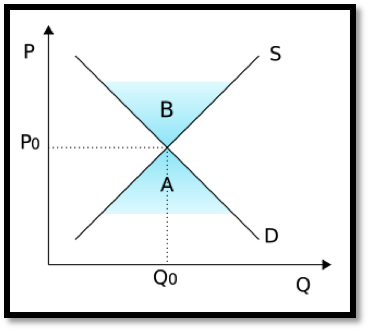
\includegraphics[width=1\linewidth]{images/sec1-1-SDcurves.png}
\end{sbspanel}%
\end{sidebyside}%
\par
\hypertarget{p-40}{}%
The vertical axis shows the price, the horizontal axis shows quantity. Both supply (S) and demand (D) are linear functions. In this diagram 'B' denotes a surplus of supply, and 'A' denotes a surplus of demand.%
\end{example}
\hypertarget{p-41}{}%
Recall, that the slope of a line through the points \(P_0=(q_0,p_0)\) and \(P_1=(q_1,p_1)\) is given by%
\begin{assemblage}{}{SlopeDef}%
\hypertarget{p-42}{}%
%
\begin{equation*}
m=\frac{rise}{run}=\frac{(p_1-p_0)}{(q_1-q_0 )}
\end{equation*}
%
\end{assemblage}
\begin{sidebyside}{1}{0.25}{0.25}{0}%
\begin{sbspanel}{0.5}%
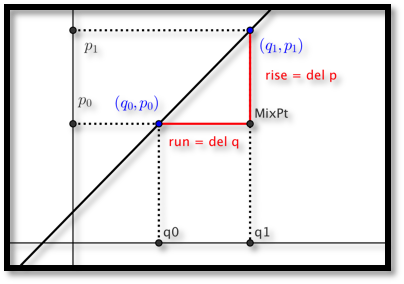
\includegraphics[width=1\linewidth]{images/sec1-1-slope.png}
\end{sbspanel}%
\end{sidebyside}%
\par
\hypertarget{p-43}{}%
There are two other forms of a line that are sometimes used. The general form of a line is a standard notation used in mathematics. The 2-point form of a line is very handy in those situations where we are not given a slope, but we are given information about two points that lie on the line.%
\begin{assemblage}{}{GeneralLinearEquations}%
\leavevmode%
\begin{sidebyside}{1}{0}{0}{0}%
\begin{sbspanel}{1}%
{\centering%
\begin{tabular}{ll}
\(a x+b y+c=0\)&The general form of a line\tabularnewline[0pt]
\(y-y_0=(y_1-y_0)/(x_1-x_0 )(x-x_0)\)&The 2-point form of a line
\end{tabular}
\par}
\end{sbspanel}%
\end{sidebyside}%
\end{assemblage}
\hypertarget{p-44}{}%
As above, in the setting of this course we may be using \(p\) (price) and \(q\) (quantity) as our variables. This would result in equations that look as follows:%
\begin{assemblage}{}{PQGeneralLinearEquations}%
\leavevmode%
\begin{sidebyside}{1}{0}{0}{0}%
\begin{sbspanel}{1}%
{\centering%
\begin{tabular}{ll}
\(a q+b p+c=0\)&The general form of a line\tabularnewline[0pt]
\(p-p_0=(p_1-p_0)/(q_1-q_0 )(q-q_0)\)&The 2-point form of a line
\end{tabular}
\par}
\end{sbspanel}%
\end{sidebyside}%
\end{assemblage}
\begin{example}{Finding four versions of a line.}{example-2}%
\hypertarget{p-45}{}%
We find that we can sell 150 widgets a day if we sell them at \textdollar{}10.  If we raise the price to \textdollar{}15, we can only sell 110 widgets a day.  Assume that there is a linear relationship between price and quantity sold.  Find the equation of the line in all four forms.%
\par
\hypertarget{p-46}{}%
\terminology{Solution}:  Writing this using our variables p (price) and q (quantity of widgets) we see that when \(p = 10\), \(q = 150\) and when \(p = 15\), \(q = 110\).  Points are (usually) given as \((q,p)\), so this means we have two point (150,10) and (110,15) on the line. We always need to find the slope of the line, and in this case%
\begin{equation*}
m=  \frac{5-10}{110-150}=  \frac{5}{-40}= \frac{-1}{8}
\end{equation*}
We are given two points, so the 2-point form of the line should be the easiest formula to find:%
\begin{equation*}
p-p_0=\frac{p_1-p_0}{q_1-q_0 }(q-q_0)
\end{equation*}
We just found the slope and we just need to pick a point \((p_0,q_0)\) to finish the problem. (Recall that \(p\) and \(q\) are the variables, so we want to leave those as they are.) In this case lets pick \((p_0,q_0)= (150,10)\). Then we get this simplified version, which is also the point-slope form of this line.%
\begin{equation*}
p-10=\frac{-1}{8}(q-150)
\end{equation*}
From here we can very easily find the slope intercept form by some straight-forward algebra: \(p-10=\frac{-1}{8}(q-150)\) implies that%
\begin{equation*}
p=\frac{-1}{8} (q-150)+10=  \frac{-1}{8} q+  \frac{150}{8}+10=  \frac{-1}{8} q+\frac{230}{8}
\end{equation*}
%
\par
\hypertarget{p-47}{}%
And finally the general form will be another exercise in algebra. We clear the fractions and put everything on one side.%
\begin{equation*}
8p+q-230=0.
\end{equation*}
%
\end{example}
\begin{example}{Finding a line from two points.}{example-3}%
\hypertarget{p-48}{}%
Suppose that a linear cost-quantity relationship exists in producing widgets.  There is a fixed cost of \textdollar{}400.  There is also a per-unit cost of \textdollar{}11.%
\leavevmode%
\begin{enumerate}[label=(\alph*)]
\item\hypertarget{li-17}{}\hypertarget{p-49}{}%
Find the equation of the line.%
\item\hypertarget{li-18}{}\hypertarget{p-50}{}%
Find the cost of making 200 widgets.%
\end{enumerate}
\hypertarget{p-51}{}%
\terminology{Solution}:%
\par
\hypertarget{p-52}{}%
1) We have one point of the form (quantity, cost) at (0, 400) from the fixed cost.  This point happens to be an intercept.  The slope of the line is \(m=11/1=11\).  We will let \(C\) stand for Cost and \(q\) stand for quantity. The general formula for a line with these variables will have the form%
\begin{equation*}
C=m q+b.
\end{equation*}
%
\par
\hypertarget{p-53}{}%
In this example \(m = 11\) and \(b = 400\), hence the equation of the line is%
\begin{equation*}
C=11 q+400
\end{equation*}
%
\par
\hypertarget{p-54}{}%
b) Using the equation form part a) we see that the cost of producing 200 widgets is%
\begin{equation*}
C=11 (200)+400=\$2,600
\end{equation*}
%
\end{example}
\begin{example}{A nonlinear function.}{example-4}%
\hypertarget{p-55}{}%
Example 4:  Sarah is paid \textdollar{}500 for working up to 40 hours per week.  For work beyond 40 hours per week she is paid \textdollar{}18\slash{}hour.%
\leavevmode%
\begin{enumerate}[label=(\alph*)]
\item\hypertarget{li-19}{}\hypertarget{p-56}{}%
Find the equation of the line.%
\item\hypertarget{li-20}{}\hypertarget{p-57}{}%
How much is she paid if she works 56 hours in a week?%
\item\hypertarget{li-21}{}\hypertarget{p-58}{}%
What is she paid for working 30 hours in a week?%
\end{enumerate}
\hypertarget{p-59}{}%
\terminology{Solution}:%
\par
\hypertarget{p-60}{}%
a) For this example we will use “designer variables”. The output will be Pay, and the input variable – the number of hours worked – will be hrs. We are told that Pay = 500 when hrs = 40. The slope of the line work beyond 40 hours is \(m=18\).  Another way to think of this is to say that there is a fixed Pay of \textdollar{}500 and a variable Pay for any hours in excess of 40: i.e. (hrs - 40). Thus, the equation of the line, according to the point-slope form is \begin{assemblage}{}{PayEquations}%
\hypertarget{p-61}{}%
%
\begin{equation*}
Pay=variable\  pay+Fixed\  pay.
\end{equation*}
%
\end{assemblage}
%
\begin{equation*}
Pay=m(hrs-40)+500=18*(hrs-40)+500.
\end{equation*}
%
\par
\hypertarget{p-62}{}%
b) The pay for working 56 hours is 18(56-40)+500=\textdollar{}788.%
\par
\hypertarget{p-63}{}%
c) The pay for working 30 hours is \textdollar{}500.  This is a trick question part of the problem.  From the text of the problem, the linear model only works for overtime, with a flat rate applying to less than 40 hours per week. Comment: The function should be written as a piecewise defined function.%
\par
\hypertarget{p-64}{}%
This question is all about the function \(f\) defined by%
\begin{equation*}
Pay=\begin{cases}
500&hrs\le 40\\
18*(hrs-40)+500&hrs>40\\
\end{cases}
\end{equation*}
%
\end{example}
\hypertarget{p-65}{}%
It can be useful when writing reports to have variables that convey some meaning. We could have called \(Pay\) \textasciigrave{}\(y\)', and \(hrs\) \textasciigrave{}\(x\)', but using the much more easily interpreted variables named Pay and hrs helps when using the formulas.%
%
%
\typeout{************************************************}
\typeout{Exercises 1.1 Exercises 1.1 Linear Functions and models}
\typeout{************************************************}
%
\begin{exercises-subsection-numberless}{Exercises 1.1 Linear Functions and models}{}{Exercises 1.1 Linear Functions and models}{}{}{exercises-set-sec-1-1}
\par\medskip\noindent%
\hypertarget{exercisegroup-1}{}%
\hypertarget{p-66}{}%
For problems 1-6, given two points in the \((q,p)\) plane and a value \(q_0\):%
\leavevmode%
\begin{enumerate}[label=(\alph*)]
\item\hypertarget{li-22}{}\hypertarget{p-67}{}%
Find the slope of the line determined by the points.%
\item\hypertarget{li-23}{}\hypertarget{p-68}{}%
Give the equation of the line determined by the points.%
\item\hypertarget{li-24}{}\hypertarget{p-69}{}%
Give the value of \(p\) predicted for \(q_0\) by the line.%
\end{enumerate}
\begin{exercisegroup}
\begin{divisionexerciseeg}{1}{}{}{exercise-1}%
\hypertarget{p-70}{}%
Points \((2,5)\) and \((6,17)\), with \(q_0=4\).%
\par\smallskip%
\noindent\textbf{Hint}.\hypertarget{hint-1}{}\quad%
\hypertarget{p-71}{}%
Find the slope and use the point-slope form%
\par\smallskip%
\noindent\textbf{Solution}.\hypertarget{solution-1}{}\quad%
\leavevmode%
\begin{enumerate}[label=(\alph*)]
\item\hypertarget{li-25}{}\hypertarget{p-72}{}%
First find the slope: \(m=  \frac{\text{change in }p}{\text{change in }q}
=  \frac{17-5}{6-2}=\frac{12}{4}=3\)%
\item\hypertarget{li-26}{}\hypertarget{p-73}{}%
Next we find the equation of the line. There are several ways to do this and two methods are outlined below.%
%
\begin{itemize}[label=\textbullet]
\item{}\hypertarget{p-74}{}%
Method 1: use the point-slope equation: \(p-p_0=m (q-q_0)\). We can choose either one of the points, so in this case we will find the line using the point \((q_0,p_0 )=(2,5)\). This gives the equation \(p-5=3 (q-2)\).%
\par
\hypertarget{p-75}{}%
Rewrite this as \(p=3q-1\)%
\item{}\hypertarget{p-76}{}%
Method 2: use the slope- intercept equation \(p=m q+b\). Use \((q,p)=(2,5)\) and \(m = 3\) and solve for \(b\): \(5=3 (2)+b\). And solving for \(b\) we have that \(b= -1\), and hence \(p=3q-1\)%
\end{itemize}
\item\hypertarget{li-29}{}\hypertarget{p-77}{}%
Evaluate at the given point.  \(p(4)=3*4-1=11\)%
\end{enumerate}
\end{divisionexerciseeg}%
\begin{divisionexerciseeg}{2}{}{}{exercise-2}%
\hypertarget{p-78}{}%
Points \((5,7)\) and \((10,7)\), with \(q_0=20\).%
\end{divisionexerciseeg}%
\begin{divisionexerciseeg}{3}{}{}{exercise-3}%
\hypertarget{p-79}{}%
Points \((20,10)\) and \((40,5)\), with \(q_0=12\).%
\par\smallskip%
\noindent\textbf{Solution}.\hypertarget{solution-2}{}\quad%
\hypertarget{p-80}{}%
Just as in problem 1 we find the slope and then find the equation of the line.%
\leavevmode%
\begin{enumerate}[label=(\alph*)]
\item\hypertarget{li-30}{}\hypertarget{p-81}{}%
First find the slope: \(m=  \frac{\text{change in }p}{\text{change in }q}
=  \frac{5-10}{40-20}=-\frac{5}{20}=-\frac{1}{4}\)%
\item\hypertarget{li-31}{}\hypertarget{p-82}{}%
Using \(p=m (q-q_0)+p_0\) with \((q_0,p_0 )=(20, 10)\) and \(m = -\frac{1}{4}\), we get \(p=-\frac{1}{4}(q-20)+10\).  Solving for \(p\) we get \(p =-\frac{1}{4}q+15\)%
\item\hypertarget{li-32}{}\hypertarget{p-83}{}%
Evaluate at the given point.  \(p(12)=-\frac{1}{4}(12)+15=12\)%
\end{enumerate}
\end{divisionexerciseeg}%
\begin{divisionexerciseeg}{4}{}{}{exercise-4}%
\hypertarget{p-84}{}%
Points \((5,62)\) and \((115,783)\), with \(q_0=415\).%
\end{divisionexerciseeg}%
\begin{divisionexerciseeg}{5}{}{}{exercise-5}%
\hypertarget{p-85}{}%
Points \((273,578)\) and \((412,6)\), with \(q_0=309\).%
\par\smallskip%
\noindent\textbf{Solution}.\hypertarget{solution-3}{}\quad%
\hypertarget{p-86}{}%
Just as in problem 1 we find the slope and then find the equation of the line.%
\leavevmode%
\begin{enumerate}[label=(\alph*)]
\item\hypertarget{li-33}{}\hypertarget{p-87}{}%
First find the slope: \(m=  \frac{\text{change in }p}{\text{change in }q}
=  \frac{578-6}{273-412}=-\frac{5}{20}=-\frac{572}{139}\)%
\item\hypertarget{li-34}{}\hypertarget{p-88}{}%
Using \(p=m (q-q_0)+p_0\) with \((q_0,p_0 )=(412, 6)\) and \(m = -\frac{572}{139}\), we get \(p=-\frac{572}{139}(q-412)+6\).  (We can combine the constant terms – the \(6\) and the \(-\frac{572}{139}*(-412)\), but leaving the equation in this form is acceptable.)%
\item\hypertarget{li-35}{}\hypertarget{p-89}{}%
Evaluate at the given point.  \(p(309)=-\frac{572}{139}(309-412)+6
=-\frac{572}{139}(-103)+6=429\frac{119}{139}\)%
\end{enumerate}
\end{divisionexerciseeg}%
\begin{divisionexerciseeg}{6}{}{}{exercise-6}%
\hypertarget{p-90}{}%
Points \((509,17)\) and \((211,132)\), with \(q_0=4\).%
\end{divisionexerciseeg}%
\end{exercisegroup}
\par\medskip\noindent
\par\medskip\noindent%
\hypertarget{exercisegroup-2}{}%
\hypertarget{p-91}{}%
For problems 7-12, start with the information given:%
\leavevmode%
\begin{enumerate}[label=(\alph*)]
\item\hypertarget{li-36}{}\hypertarget{p-92}{}%
Give the equation of the line determined by that information.%
\item\hypertarget{li-37}{}\hypertarget{p-93}{}%
Using the line, give the predicted value of \(p\) for the given \(q_0\).%
\item\hypertarget{li-38}{}\hypertarget{p-94}{}%
Give the value of \(q\) for which the predicted value of \(p\) is \(0\).%
\end{enumerate}
\begin{exercisegroup}
\begin{divisionexerciseeg}{7}{}{}{exercise-7}%
\hypertarget{p-95}{}%
A slope of \(3\), passing through \((6,3)\), with \(q_0=4\).%
\par\smallskip%
\noindent\textbf{Solution}.\hypertarget{solution-4}{}\quad%
\leavevmode%
\begin{enumerate}[label=(\alph*)]
\item\hypertarget{li-39}{}\hypertarget{p-96}{}%
Using \(p=m q+b\), we get \(3=3 (6)+b\), so \(b= -15\) and the equation of the line is \(p=3 q-15\)%
\item\hypertarget{li-40}{}\hypertarget{p-97}{}%
If \(q_0=4\), then \(p=3 q-15=3(4)-15= -3\)%
\item\hypertarget{li-41}{}\hypertarget{p-98}{}%
The predicted value of \(p\) is \(0\), when \(0=3 q-15\). Solving for \(q\) we get \(q=5\). [Comment: in part a) we could have used the point-slope for as well.]%
\end{enumerate}
\end{divisionexerciseeg}%
\begin{divisionexerciseeg}{8}{}{}{exercise-8}%
\hypertarget{p-99}{}%
A slope of \(-2\), passing through \((2,-5)\), with \(q_0=3\).%
\end{divisionexerciseeg}%
\begin{divisionexerciseeg}{9}{}{}{exercise-9}%
\hypertarget{p-100}{}%
A slope of \(12.7\), passing through \((22,183)\), with \(q_0=46\).%
\par\smallskip%
\noindent\textbf{Solution}.\hypertarget{solution-5}{}\quad%
\leavevmode%
\begin{enumerate}[label=(\alph*)]
\item\hypertarget{li-42}{}\hypertarget{p-101}{}%
Using \(p=m (q-q_0 )+p_0\)   we get \(p=12.7 (q-22)+183\).%
\item\hypertarget{li-43}{}\hypertarget{p-102}{}%
When \(q_0=46\), we get that \(p=12.7 (46-22)+183=12.7(24)+183\). And hence \(p=487.8\)%
\item\hypertarget{li-44}{}\hypertarget{p-103}{}%
The predicted value of \(p\) is \(0\), when \(0=183+12.7 (q-22)\). Solving for \(q\) we get: \(12.7 (q-22)= -183\) This implies \((q-22)= \frac{-183}{12.7}\)%
%
\begin{equation*}
q=22 -\frac{183}{12.7}=7.59
\end{equation*}
\end{enumerate}
\end{divisionexerciseeg}%
\begin{divisionexerciseeg}{10}{}{}{exercise-10}%
\hypertarget{p-104}{}%
A slope of \(-0.23\), passing through \((7.6,19.7)\), with \(q_0=59.6\).%
\end{divisionexerciseeg}%
\begin{divisionexerciseeg}{11}{}{}{exercise-11}%
\hypertarget{p-105}{}%
A slope of 0, passing through \((12.3,9.8)\), with \(q_0=74\).%
\par\smallskip%
\noindent\textbf{Solution}.\hypertarget{solution-6}{}\quad%
\leavevmode%
\begin{enumerate}[label=(\alph*)]
\item\hypertarget{li-45}{}\hypertarget{p-106}{}%
Using \(p=m (q-q_0 )+p_0\)   we get \(p=0 (q-12.3)+9.8\) or \(p=9.8\).%
\item\hypertarget{li-46}{}\hypertarget{p-107}{}%
When \(q_0=74\), we get that \(p=9.8\). (This is a constant function, and the output is going to be \(9.8\) no matter what value of \(q\) we plug in.)%
\item\hypertarget{li-47}{}\hypertarget{p-108}{}%
The predicted value of \(p\) is never  \(0\), because the predicted value of p is always 9.8.%
\end{enumerate}
\end{divisionexerciseeg}%
\begin{divisionexerciseeg}{12}{}{}{exercise-12}%
\hypertarget{p-109}{}%
A slope that is undefined, passing through \((6,3)\), explaining why part b would not make sense.%
\end{divisionexerciseeg}%
\end{exercisegroup}
\par\medskip\noindent
\par\medskip\noindent%
\hypertarget{exercisegroup-3}{}%
\hypertarget{p-110}{}%
For problems 13-18, start with the equation given:%
\leavevmode%
\begin{enumerate}[label=(\alph*)]
\item\hypertarget{li-48}{}\hypertarget{p-111}{}%
Give the slope of the line or say that the slope is undefined.%
\item\hypertarget{li-49}{}\hypertarget{p-112}{}%
Give the intercepts of the line with the axes.%
\item\hypertarget{li-50}{}\hypertarget{p-113}{}%
Give two points that are on the line but not on the axes.%
\end{enumerate}
\begin{exercisegroup}
\begin{divisionexerciseeg}{13}{}{}{exercise-13}%
\hypertarget{p-114}{}%
\(3 p+2 q=6\).%
\par\smallskip%
\noindent\textbf{Solution}.\hypertarget{solution-7}{}\quad%
\leavevmode%
\begin{enumerate}[label=(\alph*)]
\item\hypertarget{li-51}{}\hypertarget{p-115}{}%
Solve for \(p\) so we can read off the slope more easily:  \(p= -2/3 q+2\). Hence the slope is \(m= -2/3\)%
\item\hypertarget{li-52}{}\hypertarget{p-116}{}%
To get the \(p\)-intercept we set \(q=0\), so that \(3 p=6\), and we get \(p=2\) To get the \(q\)-intercept we set \(p=0\), so that \(2q=6\), and we get \(q=3\)%
\item\hypertarget{li-53}{}\hypertarget{p-117}{}%
We can pick any two values for \(q\) (except \(0\) and \(3\) because those are intercepts), so arbitrarily pick some values: say \(q=1\) and \(q=-1\). If \(q=1\), then \(3 p+2=6\), and hence  \(p=4/3\) so the point would be \((q,p)=(1,4/3)\) If \(q=-1\), then \(3 p-2=6\), and hence  \(p=8/3\) so the point would be \((q,p)=(-1,8/3  )\)%
\end{enumerate}
\end{divisionexerciseeg}%
\begin{divisionexerciseeg}{14}{}{}{exercise-14}%
\hypertarget{p-118}{}%
\(7 p-4 q+14=0\).%
\end{divisionexerciseeg}%
\begin{divisionexerciseeg}{15}{}{}{exercise-15}%
\hypertarget{p-119}{}%
\(y=5\).%
\par\smallskip%
\noindent\textbf{Solution}.\hypertarget{solution-8}{}\quad%
\leavevmode%
\begin{enumerate}[label=(\alph*)]
\item\hypertarget{li-54}{}\hypertarget{p-120}{}%
The slope is \(0\)%
\item\hypertarget{li-55}{}\hypertarget{p-121}{}%
The y-intercept is \(y = 5\). There is no \(x\)-intercept%
\item\hypertarget{li-56}{}\hypertarget{p-122}{}%
No matter what \(x\) we choose the \(y\) value will always be \(5\). So we can pick any two values of \(x\) (not \(0\) to avoid the intercept). For instance \((x,y)=(-20,5)\), \((x,y)=(-2,5)\), \((x,y)=(7,5)\), etc are all points on the line.%
\end{enumerate}
\end{divisionexerciseeg}%
\begin{divisionexerciseeg}{16}{}{}{exercise-16}%
\hypertarget{p-123}{}%
\(x=3\).%
\end{divisionexerciseeg}%
\begin{divisionexerciseeg}{17}{}{}{exercise-17}%
\hypertarget{p-124}{}%
\(y=4(x-3)+9\).%
\par\smallskip%
\noindent\textbf{Solution}.\hypertarget{solution-9}{}\quad%
\leavevmode%
\begin{enumerate}[label=(\alph*)]
\item\hypertarget{li-57}{}\hypertarget{p-125}{}%
The slope is \(4\)%
\item\hypertarget{li-58}{}\hypertarget{p-126}{}%
To get the \(y\)-intercept we set \(y=0\), so that \(y=4(-3)+9=-3\),%
\par
\hypertarget{p-127}{}%
To get the \(x\)-intercept we set \(y=0\), so that \(0=4(x-3)+9\).  Solve for \(x\) and we get \(x-3=-\frac{9}{4}\) and \(x=3-\frac{9}{4}=\frac{3}{4}\)%
\item\hypertarget{li-59}{}\hypertarget{p-128}{}%
Avoiding the intercepts we can choose \(x\) to be any number other than \(x = 0\) and \(x=3/4\).  We may look for nice values of \(x\) that make the arithmetic come out nice: for example choose \(x=3\) and \(x=4\). When \(x=3\), \(y=9\), and we get the point \((x,y)=(3,9)\). When \(x=4\), \(y=13\), and we get the point \((x,y)=(4,13)\).%
\end{enumerate}
\end{divisionexerciseeg}%
\begin{divisionexerciseeg}{18}{}{}{exercise-18}%
\hypertarget{p-129}{}%
\(112 p+257 q=4783\).%
\end{divisionexerciseeg}%
\end{exercisegroup}
\par\medskip\noindent
\begin{divisionexercise}{19}{}{}{exercise-19}%
\hypertarget{p-130}{}%
Suppose that the relationship between price and quantity of widgets sold is linear.  When the price is \textdollar{}23, we can sell 4783 widgets.  If we raise the price to \textdollar{}27, we can only sell 4295 widgets.  Find the equation of the line.%
\par\smallskip%
\noindent\textbf{Solution}.\hypertarget{solution-10}{}\quad%
\hypertarget{p-131}{}%
The information tells us we have two points: \((q,p)=(4783,23)\)  and \((q,p)=(4295,27)\). (Note that in business the quantity \(q\) is usually the input and price \(p\) is usually the output.)%
\par
\hypertarget{p-132}{}%
Next we need the slope: \(m=  (27-23)/(4295-4783)=4/(-488)=-1/122\)%
\par
\hypertarget{p-133}{}%
Using \(p-p_0=m (q-q_0 )\)   we get \(p-23=-1/122  (q-4783)\). We can rewrite the latter as \(p=23-1/122  (q-4783)\).%
\end{divisionexercise}%
\begin{divisionexercise}{20}{}{}{exercise-20}%
\hypertarget{p-134}{}%
Suppose that the relationship between price and quantity of gizmo kits we can buy is linear.  When the price is \textdollar{}15, we can buy 6000 gizmo kits.  If we lower the price we will pay to \textdollar{}13, we can only buy 4500 kits.  Find the equation of the line.%
\end{divisionexercise}%
\end{exercises-subsection-numberless}
\end{sectionptx}
%
%
\typeout{************************************************}
\typeout{Section 1.2 Functions in the Business setting}
\typeout{************************************************}
%
\begin{sectionptx}{Functions in the Business setting}{}{Functions in the Business setting}{}{}{sec-1-2-FunctionsBusinessSetting}
\hypertarget{p-135}{}%
\href{./Examples/Section-1-2-Examples.xlsx}{Link to worksheets used in this section}%
\par
\hypertarget{p-136}{}%
Not all functions we encounter in a business setting are linear. There are several other families of functions we should (re-) familiarize ourselves with. These models include:\leavevmode%
\begin{itemize}[label=\textbullet]
\item{}Quadratic functions%
\item{}Exponential functions%
\item{}Logistic functions%
\item{}Normal distribution functions%
\item{}Sinusoidal functions%
\end{itemize}
%
\par
\hypertarget{p-137}{}%
\terminology{Quadratic Functions}%
\par
\hypertarget{p-138}{}%
\terminology{Quadratic functions} should be very familiar from previous mathematics courses. They are of the form \(y=a x^2+b x+c\). These are our standard parabolas.%
\par
\hypertarget{p-139}{}%
In business we encounter quadratic equations when we study revenue and profit functions. Recall from your economics course that:%
\begin{equation*}
Revenue=price*quantity=p*q
\end{equation*}
In some of the models we will investigate later in the course price will be a linear function. We will assume \(Price=m q+b\). This implies that%
\begin{equation*}
Revenue=(m q+b)*q=m q^2+b q
\end{equation*}
If \(m > 0\), then the revenue function will look like a parabola that opens up. If \(m \lt 0,\) then the revenue function will look like a parabola that opens down.%
\begin{sidebyside}{1}{0.25}{0.25}{0}%
\begin{sbspanel}{0.5}%
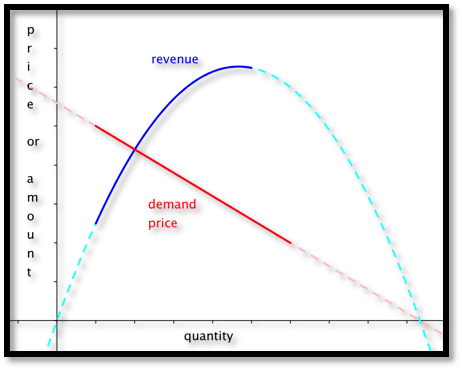
\includegraphics[width=1\linewidth]{images/sec1-2-QuadraticFunctions.png}
\end{sbspanel}%
\end{sidebyside}%
\par
\hypertarget{p-140}{}%
For a quadratic model we are often very interested in the coordinates of the vertex, and any possible zeros. For the general equation \(y=a x^2+b x+c\) the sign of the coefficient of \(x^2\), \(a\), will determine if we have a maximum or a minimum. If \(a\) is positive, the parabola opens up and the vertex will be a minimum. If \(a\) is negative, the parabola opens down and the vertex will be a maximum.%
\par
\hypertarget{p-141}{}%
Recall that we can find the zeros of a quadratic by using the quadratic equation.%
\begin{equation*}
roots\ or\ zeroes  =  
\frac{-b\pm\sqrt{b^2-4ac}}{2a}
\end{equation*}
From this equation we see that the vertex must be located at \(x= -b/(2a.)\). The discriminant (the term underneath the radical sign determines if there are 0, 1, or 2 roots.%
\leavevmode%
\begin{itemize}[label=\textbullet]
\item{}\hypertarget{p-142}{}%
If \(b^2-4ac>0\), then there are 2 roots.%
\item{}\hypertarget{p-143}{}%
If \(b^2-4ac=0\), then there is 1 root (the vertex will touch the axis)%
\item{}\hypertarget{p-144}{}%
If \(b^2-4ac\lt 0\), then there are no roots. This means the entire graph must lie above the \(x\)-axis (\(a > 0\)) or below the \(x\)-axis (\(a \lt 0\)).%
\end{itemize}
\hypertarget{p-145}{}%
Sometimes we may need more general polynomials in a model, with an equation of the form \(f(x)=a_n x^n+\cdots+a_1 x+a_0\).  In such cases we remember that the number of turning points of the graph can be no more than \(n-1\).%
\par
\hypertarget{p-146}{}%
\terminology{Exponential functions}%
\par
\hypertarget{p-147}{}%
The \terminology{exponential model}, with an equation of the form \(f(t)=p*e^t\). Sometimes the exponential function \(e^t\) is denoted by \(exp(t)\). Excel will use this format, so it is worth looking at the notation in this case. \(f(t)=p*e^{rt}\) can also be written as  \(f(t)=p*exp(r t)\)%
\par
\hypertarget{p-148}{}%
Math books (and Excel) like using a base of \(e\) because it makes the mathematics easier when we do calculus, so the equation is written as \(f(t)=p*e^{rt}\) or \(f(t)=p*exp(r t)\). However, in real world applications we tend to use \(A=pR^t\) and make the equation \(f(t)=p*R^t\).  (The reader is warned that \(R=e^r\) and both \(R\) and \(r\) are referred to as the \terminology{rate}.  You will have to use the context to tell them apart.)%
\par
\hypertarget{p-149}{}%
Exponential functions are used for proportional growth or decay.  In business, compound interest is given as an exponential function. In particular, if \(P\) is the principal and \(r\) is the interest rate "compounded continuously" (expressed as a decimal), then the amount \(A\) after time \(t\) is given by \(A=P e^rt\). The relationship (in general) between a \terminology{future value} (FV) and the \terminology{present value} (PV) given an interest rate \(r\) per period, with \(t\) being the number of compounding periods is given by:%
\begin{assemblage}{}{FutureValueDef}%
\hypertarget{p-150}{}%
%
\begin{equation*}
Future Value: FV=PV*(1+r)^t
\end{equation*}
%
\end{assemblage}
\hypertarget{p-151}{}%
It is also useful in determining a fair value today of a promised future payout. The sign of the rate will determine if the graph turns up or down.%
\par
\hypertarget{p-152}{}%
When modeling real world behavior, we often know some special features of the problem. For instance, we may know that our present value is \textdollar{}2,000 and that we would like the future value to be \textdollar{}10,000 after 10 years. The question would be what function would describe such a model? A method commonly used to solve such a problem is to plug in the values we are given and see if we can determine what the remaining quantities should be. We know that \(FV=PV*(1+r)^t\). The extra information tells us PV = 2000, and when t = 10 we know that \(FV=2000*(1+r)^{10}=10,000\). This is enough information to solve for r. Dividing both sides by 2000 shows that \((1+r)^{10}=5\). To solve this equation we need rules of exponents. We obtain: \(1+r=5^{1⁄10}\), and hence \(r= 5^{1/10}-1= 0.1746\). This means that to obtain such a growth we would need a rate of growth of about 17.46\%. The function modeling that growth would be \(FV=2000*(1.1746)^t\). In general we can set up equations and solve for the unknown quantities.%
\par
\hypertarget{p-153}{}%
\terminology{Logistic Functions}%
\par
\hypertarget{p-154}{}%
The exponential model assumes growth without end.  That is impossible in most business situations.  Instead there is typically a point where the market is saturated.  The alternative model says that the rate of change is proportional both to the current quantity and to the distance from the theoretical maximum value.  This is called logistic growth.  A typical formula for \terminology{logistic growth} given an interest rate \(r\), market saturation point \(M\), and constant a depending on the problem is%
%
\begin{equation*}
f(x)=  \frac{M}{1+a e^{-rx}} 
\end{equation*}
\hypertarget{p-155}{}%
In Excel we would write this function as: f(x)=M\slash{}(1+a exp(-r x)). Using Excel it is fairly easy to create a table and graph a logistic function.%
\begin{sidebyside}{1}{0.25}{0.25}{0}%
\begin{sbspanel}{0.5}%
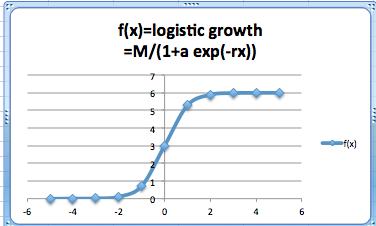
\includegraphics[width=1\linewidth]{images/sec1-2-LogisticFunction.png}
\end{sbspanel}%
\end{sidebyside}%
\par
\hypertarget{p-156}{}%
\terminology{Sinusoidal Functions}%
\par
\hypertarget{p-157}{}%
The \terminology{sinusoidal model} is for data that repeats on a natural cycle.  Typical examples would include need for heating oil, electricity for air conditioning, and sales for seasonal items such as Christmas.  The typical equation is%
%
\begin{equation*}
f(x)=M+A*sin(2\pi*(x-shift)/period),
\end{equation*}
\hypertarget{p-158}{}%
where the mean \(M\) is the average value, the amplitude \(A\) is the distance from the mean to the maximum, the period is the length of time till the cycle repeats, and the shift is where we start the cycle for \(x=0\). With an appropriate shift we can interchange the sine and cosine functions.  (The functions \(sin(x)\) and \(cos(x)\) arise from trigonometry.)  In this course, we will not focus on trigonometric functions and their properties.  We are only concerned with having a periodic function for seasonal variations.%
\begin{sidebyside}{1}{0.25}{0.25}{0}%
\begin{sbspanel}{0.5}%
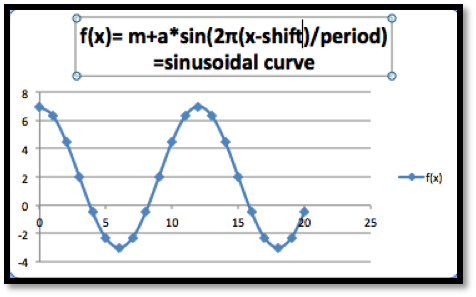
\includegraphics[width=1\linewidth]{images/sec1-2-SinCurve.png}
\end{sbspanel}%
\end{sidebyside}%
\par
\hypertarget{p-159}{}%
\terminology{Normal Distribution Functions}%
\par
\hypertarget{p-160}{}%
The \terminology{normal distribution} or \terminology{bell curve} is used because many populations follow a normal distribution on many scales.  The equation%
%
\begin{equation*}
f(x)=a e^{-\left(\frac{(x-m)}{s}\right)^2} 
\end{equation*}
\hypertarget{p-161}{}%
looks a bit intimidating, but we will be able to use the power of a spreadsheet to easily handle it.%
\par
\hypertarget{p-162}{}%
In retail, there are several examples of items that follow a normal distribution. In a store selling shoes for women for instance, we would expect to see that some sizes are more prevalent than others. This would be a factor in determining what sizes to have in stock, and at what quantities. The typical scenario in which we will be using this curve model is one where we ask what range of sizes do we need to cover for the population in an area to be large enough to justify a specialty store.%
\begin{sidebyside}{1}{0.25}{0.25}{0}%
\begin{sbspanel}{0.5}%
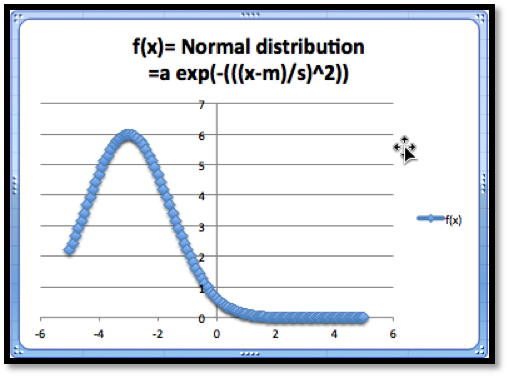
\includegraphics[width=1\linewidth]{images/sec1-2-NormalCurve.png}
\end{sbspanel}%
\end{sidebyside}%
\par
\hypertarget{p-163}{}%
The normal distribution function has certain interesting features. The graph shows a maximum value. The maximum occurs when \(x = m\). And when \(x = m\), we know that%
%
\begin{equation*}
f(x)=a e^{\left(\frac{-(m-m)}{s}\right)^2}=a e^0=a*1=a,
\end{equation*}
\hypertarget{p-164}{}%
hence the maximum value is \(a\).%
\par
\hypertarget{p-165}{}%
There are a few more models that will show up from time to time and are worth mentioning.%
\par
\hypertarget{p-166}{}%
\terminology{Inversely Proportional Functions}%
\par
\hypertarget{p-167}{}%
If we see the phrase that two quantities are inversely proportional, it means that \(f(x)\) is a constant times \(1/x\).  We might expect to use such a model when a fixed amount of money will be spent to acquire all of a given product.  Thus we may see it used to describe price as a function of supply.%
\begin{sidebyside}{1}{0.25}{0.25}{0}%
\begin{sbspanel}{0.5}%
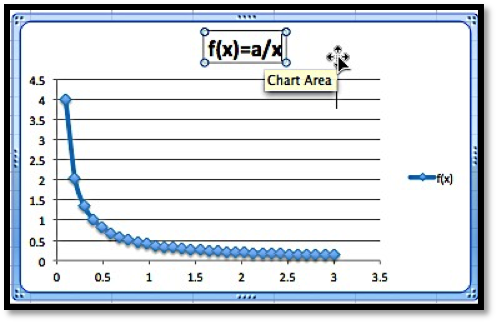
\includegraphics[width=1\linewidth]{images/sec1-2-InverseCurve.png}
\end{sbspanel}%
\end{sidebyside}%
\par
\hypertarget{p-168}{}%
\terminology{Logarithmic Functions}%
\par
\hypertarget{p-169}{}%
The \terminology{logarithmic model} looks at equations of the form \(f(x)=a*\ln (x)+b\) or \(f(x)=a*\ln (Bx)\).  This model shows up in two ways.  It can be obtained as the accumulation of a quantity that is inversely proportional to our variable.  It also shows up as the inverse of the exponential model.  (If \(y\) is described as an exponential function of \(x\), then \(x\) is a logarithmic function of \(y\).)%
\begin{sidebyside}{1}{0.25}{0.25}{0}%
\begin{sbspanel}{0.5}%
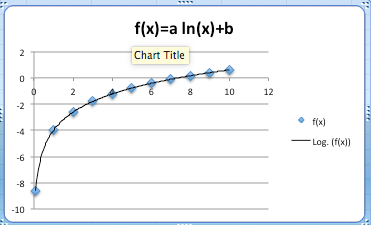
\includegraphics[width=1\linewidth]{images/sec1-2-LogCurve.png}
\end{sbspanel}%
\end{sidebyside}%
%
%
\typeout{************************************************}
\typeout{Exercises 1.2 Exercises  Functions in the Business Setting}
\typeout{************************************************}
%
\begin{exercises-subsection-numberless}{Exercises  Functions in the Business Setting}{}{Exercises  Functions in the Business Setting}{}{}{exercises-set-sec-1-2}
\hypertarget{p-170}{}%
For each model, some features of the graph are listed.  Describe how to change each feature by changing the parameters of the model.  (E.g., With the linear model, \(f(x)=a x+b\), the parameters are \(a\) and \(b\).  The place where the line intercepts the \(x\)-axis is \(–b/a\), so any \(x\)-intercept can be produced with \(a=-1\) and \(b\) equal to the desired value.)%
\begin{divisionexercise}{1}{}{}{exercise-21}%
\hypertarget{p-171}{}%
For a linear model, \(f(x)=a x+b\), how do I get a graph with\leavevmode%
\begin{enumerate}[label=(\alph*)]
\item\hypertarget{li-68}{}\hypertarget{p-172}{}%
A positive \(y\)-intercept?%
\item\hypertarget{li-69}{}\hypertarget{p-173}{}%
A negative slope?%
\end{enumerate}
%
\par\smallskip%
\noindent\textbf{Solution}.\hypertarget{solution-11}{}\quad%
\leavevmode%
\begin{enumerate}[label=(\alph*)]
\item\hypertarget{li-70}{}\hypertarget{p-174}{}%
How to obtain a positive \(y\)-intercept. - The \(y\)-intercept is determined by \(b\), so we just let \(b\gt 0\).%
\item\hypertarget{li-71}{}\hypertarget{p-175}{}%
How to obtain a negative slope. - The slope is determined by \(a\) in the formula above, so we let \(a\lt 0\)%
\end{enumerate}
\end{divisionexercise}%
\begin{divisionexercise}{2}{}{}{exercise-22}%
\hypertarget{p-176}{}%
Suppose we are working with a quadratic model, \(f(x)=a x^2+b x+c\)\leavevmode%
\begin{enumerate}[label=(\alph*)]
\item\hypertarget{li-72}{}\hypertarget{p-177}{}%
How do we get a graph, that points down? (i.e. a graph that has a maximum)?%
\item\hypertarget{li-73}{}\hypertarget{p-178}{}%
How will we know if the graph of the function intercepts the \(x\)-axis at two positive values?%
\end{enumerate}
%
\end{divisionexercise}%
\begin{divisionexercise}{3}{}{}{exercise-23}%
\hypertarget{p-179}{}%
For a quadratic model, \(f(x)=a x^2+b x+c\), How do I get a graph where the vertex has \(x=5\)?%
\par\smallskip%
\noindent\textbf{Solution}.\hypertarget{solution-12}{}\quad%
\hypertarget{p-180}{}%
Quadratics are parabolas and the zeros (if they exist) are at \(x=  \frac{-b\pm \sqrt{b^2-4ac}}{2a}\).%
\par
\hypertarget{p-181}{}%
The vertex is always located at \(x=  \frac{-b}{2a}\). So if the vertex is to be at \(x = 5\) we need to make sure \(\frac{-b}{2a}=5\). There are many ways to do this (there are infinitely many different parabolas with their vertex located at x = 5). One possible solution would be to let \(b = -10\) and \(a = 1\).%
\end{divisionexercise}%
\begin{divisionexercise}{4}{}{}{exercise-24}%
\hypertarget{p-182}{}%
For a polynomial model, \(f(x)=a_n x^n+\cdots+a_1 x+a_0\), how do I get a graph that goes up at both ends?%
\end{divisionexercise}%
\begin{divisionexercise}{5}{}{}{exercise-25}%
\hypertarget{p-183}{}%
For an exponential model, \(f(x)=P*\exp(r x)\), how do I get a graph with \(f(0)=100\), that goes to zero as x gets large?%
\par\smallskip%
\noindent\textbf{Solution}.\hypertarget{solution-13}{}\quad%
\leavevmode%
\begin{itemize}[label=\textbullet]
\item{}\hypertarget{p-184}{}%
\(f(0)=P*\exp(0)= P\), so if  \(f(0)=100\) we know that \(P=100\).%
\item{}\hypertarget{p-185}{}%
If \(f\) goes to 0 as \(x\) gets large it must be an exponential decay function which means that the coefficient \(r\) must be negative.%
\end{itemize}
\end{divisionexercise}%
\begin{divisionexercise}{6}{}{}{exercise-26}%
\hypertarget{p-186}{}%
For an exponential model, \(f(x)=P*\exp(-r x)+b\), how do I get a graph where \(f(x)\) goes to 10 as \(x\) gets large, \(f(0)=1\), and \(f(10)\) is at least \(9\)?%
\end{divisionexercise}%
\begin{divisionexercise}{7}{}{}{exercise-27}%
\hypertarget{p-187}{}%
For a logistic growth model, \(f(x)=\frac{M}{1+a \exp(-r*t)}\), how do I get a graph where \(f(x)\) goes to \(10\) as \(x\) gets large, \(f(0)=1\), and \(f(10)\) is at least \(9\)?%
\par\smallskip%
\noindent\textbf{Solution}.\hypertarget{solution-14}{}\quad%
\hypertarget{p-188}{}%
We have several conditions here that need to be met. We use them to find our parameters one at a time.%
\leavevmode%
\begin{itemize}[label=\textbullet]
\item{}\hypertarget{p-189}{}%
\(f(x)\) goes to \(10\) as \(x\) gets large. If  \(-r\gt 0\), then \(a\exp(-r*x)\) gets very large as \(x\) gets large which would send \(f\) down to \(0\), but \(f\) goes to \(10.\) So we know that \(-r\lt 0\).%
\par
\hypertarget{p-190}{}%
When \(-r\lt 0\), \(\exp(-r*x)\) goes to \(0\) for large \(x\). So the whole equation must go to \(M\). Hence \(M=10\)%
\item{}\hypertarget{p-191}{}%
\(f(0)=1\). When \(x = 0\) we get \(f(x)=M/(1+a \exp(0) )=M/(1+a)=10/(1+a)=1\), Hence \(a = 9\)%
\item{}\hypertarget{p-192}{}%
\(f(10)\) is at least \(9\). With \(M = 10\) and  \(a = 9\) we have that \(f(10)=10/(1+9 \exp(-r*10) )\gt 9\) This implies that \(1+9 \exp(-r*10)\lt 10/9\) and hence \(\exp(-r*10)\lt 1/81\) This means that  \(r\gt -1/10  \ln(1/81)= 0.44\)%
\end{itemize}
\end{divisionexercise}%
\begin{divisionexercise}{8}{}{}{exercise-28}%
\hypertarget{p-193}{}%
For a sinusoidal model, \(f(x)=M+A \sin(2\pi(x+shift)/period)\), based on seasonal change through the year, if \(x\) is measured in months, what value should period have?%
\end{divisionexercise}%
\begin{divisionexercise}{9}{}{}{exercise-29}%
\hypertarget{p-194}{}%
For a normal model, \(f(x)=a \exp\left(-\left(\frac{x-m}{s}\right)^2\right)\), how do I produce a graph with a high point at \((7, 20)\), and the value of \(f(4)\) between 1 and 2?  (You need to use trial and error on this problem.)%
\par\smallskip%
\noindent\textbf{Solution}.\hypertarget{solution-15}{}\quad%
\leavevmode%
\begin{itemize}[label=\textbullet]
\item{}\hypertarget{p-195}{}%
The high point of the graph occurs when \(\frac{x-m}{s}=0\). This happens at \(x = 7\), so this means that \(m = 7\) as well.%
\item{}\hypertarget{p-196}{}%
Once we know that \(m = 7\), then \(f(7)=a \exp\left(-\left(\frac{7-7}{s}\right)^2 \right)=a \exp(0)=a\) But \(f(7)=20\), so \(a = 20\).  This means that \(f(x)=20 \exp\left(-\left(\frac{x-7}{s}\right)^2\right)\).%
\item{}\hypertarget{p-197}{}%
If the value of \(f(4)\) is between \(1\) and \(2\), \(f(4)=20 \exp\left(-\left(\frac{4-7}{s}\right)^2\right)\) is between \(1\) and \(2\). We can solve for \(s\)%
\begin{equation*}
1\lt 20 \exp\left(-\left(\frac{4-7}{s}\right)^2\right)\lt 2
\end{equation*}
%
\begin{equation*}
1/20\lt \exp\left(-\left(\frac{4-7}{s}\right)^2\right)\lt 1/10
\end{equation*}
%
\begin{equation*}
\ln (1/20)\lt \left(-\left(\frac{4-7}{s}\right)^2\right)\lt \ln (1/10)
\end{equation*}
%
\begin{equation*}
\ln (1/20)\lt \frac{-9}{s^2}\lt \ln (1/10)
\end{equation*}
and hence%
\begin{equation*}
2.3026\lt \frac{9}{s^2} \lt 2.996
\end{equation*}
So  \(s^2\gt \frac{9}{2.996}\) and  \(s^2\lt\frac{9}{2.3026} \). Hence \(1.734\lt s\lt 1.977\).%
\end{itemize}
\end{divisionexercise}%
\begin{divisionexercise}{10}{}{}{exercise-30}%
\hypertarget{p-198}{}%
For a normal model, \(f(x)=a \exp\left(-\left(\frac{x-m}{s}\right)^2\right)\), how do I produce a graph with a high point at \((7, 20)\), and the value of \(f(1)\) between 1 and 2?  (You need to use trial and error on this problem.)%
\end{divisionexercise}%
\begin{divisionexercise}{11}{}{}{exercise-31}%
\hypertarget{p-199}{}%
For the power model, \(f(x)=a x^b\), how do I produce a graph with \(f(1)=5\) and \(f(3)=1\)?%
\par\smallskip%
\noindent\textbf{Solution}.\hypertarget{solution-16}{}\quad%
\hypertarget{p-200}{}%
\(f(1)=5\) means that \(a 1^b=a=5\).%
\par
\hypertarget{p-201}{}%
\(f(3)=1\) means that \(a x^b=5*3^b=1\) hence \(3^b=0.2\) and hence \(\ln(3^b )=\ln(0.2)\).%
\par
\hypertarget{p-202}{}%
So \(b \ln(3)=\ln(0.2)\) which implies that \(b=\ln(0.2)/\ln(3) \approx -1.465\).%
\end{divisionexercise}%
\begin{divisionexercise}{12}{}{}{exercise-32}%
\hypertarget{p-203}{}%
For the inversely proportional model, \(f(x)=a/x\), how do I produce a graph with \(f(1) \lt 0\) and \(f(3)=-5?\)%
\end{divisionexercise}%
\begin{divisionexercise}{13}{}{}{exercise-33}%
\hypertarget{p-204}{}%
For the logarithmic model, \(f(x)=a \ln(x)\) how do I produce a graph with \(f(e)=3\)?%
\par\smallskip%
\noindent\textbf{Solution}.\hypertarget{solution-17}{}\quad%
\hypertarget{p-205}{}%
\(f(e)=a \ln(e)=a (1)= a\), hence \(a = 3\)%
\end{divisionexercise}%
\hypertarget{p-206}{}%
Exercises 14-21) For each situation, explain which model you would use for each situation (linear, quadratic, etc.).  Be sure to explicitly mention what you are using as the free variable (the equivalent of x), what you are using as the dependent variable (the equivalent of y), and why that model makes sense in the given situation.%
\begin{divisionexercise}{14}{}{}{exercise-34}%
\hypertarget{p-207}{}%
The cost of producing an amount of a product is the sum of the fixed costs, like warehouse rent, and the variable costs, like labor and materials, which we can assume to be the same for each unit produced.%
\end{divisionexercise}%
\begin{divisionexercise}{15}{}{}{exercise-35}%
\hypertarget{p-208}{}%
When looking at revenue, we can assume that sales will be linear function of the price of the object.%
\par\smallskip%
\noindent\textbf{Solution}.\hypertarget{solution-18}{}\quad%
\hypertarget{p-209}{}%
Using a linear model we get  \(sales=m *price+b\).%
\par
\hypertarget{p-210}{}%
Price is the free variable (the input) and sales is the dependent variable (the output)%
\end{divisionexercise}%
\begin{divisionexercise}{16}{}{}{exercise-36}%
\hypertarget{p-211}{}%
The amount I expect to be able to withdraw from an account at a future date, assuming that interest is compounded continuously and is fixed.%
\end{divisionexercise}%
\begin{divisionexercise}{17}{}{}{exercise-37}%
\hypertarget{p-212}{}%
The amount of time it takes an investment to double assuming a fixed interest rate.%
\par\smallskip%
\noindent\textbf{Solution}.\hypertarget{solution-19}{}\quad%
\hypertarget{p-213}{}%
The Future value is given by \(FV=PV*(1+r)^t\)%
\par
\hypertarget{p-214}{}%
Here the Future value (\(FV\)) will be the input (it will be \(2*PV\)) and the output will be the time \(t\).%
\end{divisionexercise}%
\begin{divisionexercise}{18}{}{}{exercise-38}%
\hypertarget{p-215}{}%
The amount of electricity needed for air conditioners in a Washington, D.C. at various times of the year.%
\end{divisionexercise}%
\begin{divisionexercise}{19}{}{}{exercise-39}%
\hypertarget{p-216}{}%
The amount of metal needed to build a fuel tank as a function of the amount of fuel to be stored.%
\par\smallskip%
\noindent\textbf{Solution}.\hypertarget{solution-20}{}\quad%
\hypertarget{p-217}{}%
Volume is 3-dimensional and the metal would be related to the surface area – which is 2-dimensional – so the formula would be something like:%
%
\begin{equation*}
Amount\ of\ metal=K*(Volume)^{3/2}
\end{equation*}
\hypertarget{p-218}{}%
\(Volume\) is the input, the \(K\) is some constant and \(Amount\ of\ Metal\) is the output.%
\end{divisionexercise}%
\begin{divisionexercise}{20}{}{}{exercise-40}%
\hypertarget{p-219}{}%
The total length of booms needed to contain an oil spill as a function of the size of the spill.%
\end{divisionexercise}%
\begin{divisionexercise}{21}{}{}{exercise-41}%
\hypertarget{p-220}{}%
The monthly sales of a hot new electronic device in a country.%
\par\smallskip%
\noindent\textbf{Solution}.\hypertarget{solution-21}{}\quad%
\hypertarget{p-221}{}%
Sales will likely increase a lot initially, but then level out. So a logistic equation may be a reasonable model.%
%
\begin{equation*}
f(x)=  M/(1+a e^{-rx} )
\end{equation*}
\end{divisionexercise}%
\begin{divisionexercise}{22}{}{}{exercise-42}%
\hypertarget{p-222}{}%
The distribution of sales of pairs of pants by leg length.%
\end{divisionexercise}%
\end{exercises-subsection-numberless}
\end{sectionptx}
%
%
\typeout{************************************************}
\typeout{Section 1.3 Introduction to Excel Spreadsheets}
\typeout{************************************************}
%
\begin{sectionptx}{Introduction to Excel Spreadsheets}{}{Introduction to Excel Spreadsheets}{}{}{sec-1-3-IntroExcelSpreadsheets}
\hypertarget{p-223}{}%
\href{./Examples/Section-1-3-Examples.xlsx}{Link to worksheets used in this section}%
\par
\hypertarget{p-224}{}%
This book will rely heavily upon the use of Excel, since it is the standard mathematical tool used in the business world.  (More precisely, the spreadsheet is the standard tool, and Excel is currently the de facto standard brand.  Most of this text can easily be used with other spreadsheets.) However, we do not assume that the student has worked with Excel previously. Throughout the course we will introduce those features of Excel we need to do mathematics and model the business problems we encounter.%
\par
\hypertarget{p-225}{}%
While introducing Excel, we will also introduce rules of “Good Excel practice.”  In a business environment, spreadsheets should be written so that someone else can easily understand the worksheet, and maintain it for future use. You should assume those same standards when submitting work in Excel.%
\par
\hypertarget{p-226}{}%
This section is meant as an introduction to several standard features of Excel we will use often. These include:%
\leavevmode%
\begin{itemize}[label=\textbullet]
\item{}\hypertarget{p-227}{}%
\terminology{Basic Arithmetic} such as add, subtract, multiply etc.%
\item{}\hypertarget{p-228}{}%
\terminology{Show formulas}: allows us to check if the formulas in the cells are what they should be.%
\item{}\hypertarget{p-229}{}%
\terminology{Quick fill}: this feature takes a pattern and fills it across a column or a row.%
\item{}\hypertarget{p-230}{}%
\terminology{Relative and Absolute Reference}: when do we refer to a fixed cell and when does the reference depend on our place in the spreadsheet?%
\item{}\hypertarget{p-231}{}%
\terminology{SUM()}: Adding a large number of cells can be efficiently done with this feature.%
\end{itemize}
\hypertarget{p-232}{}%
\terminology{Basic Arithmetic, show formulas and quick fill.}%
\par
\hypertarget{p-233}{}%
We start with an example that covers basic arithmetic.  Assume we are given the following worksheet:%
\begin{sidebyside}{1}{0.25}{0.25}{0}%
\begin{sbspanel}{0.5}%
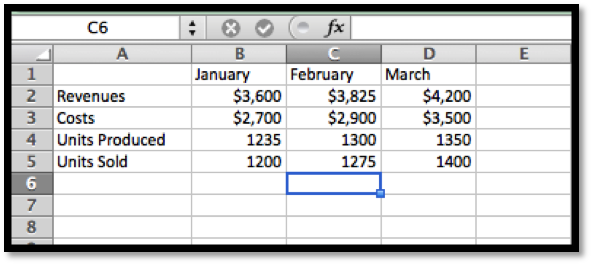
\includegraphics[width=1\linewidth]{images/sec1-3-1BasicData.png}
\end{sbspanel}%
\end{sidebyside}%
\par
\hypertarget{p-234}{}%
From data we would like to compute the figures for the quarter (add the three months), the monthly profit (revenues-cost), and the monthly unit costs (costs\slash{} units sold).%
\par
\hypertarget{p-235}{}%
With the formula ribbon, we go to show and select \terminology{Show Formulas}.  Since we want the worksheet to be readable by others, we add labels for the quantities we are computing, and in each cell we enter the formula for the quantity.   The formula bar tells us which cell has been selected and the formula for that cell.   It is generally easier to edit a formula by using the formula bar.%
\par
\hypertarget{p-236}{}%
In this example, we have used several different ways of writing the formula.  In cells E2, B6, and B7 we simply typed in the equation like we would on a calculator.  Thus the profit for January is Revenues – Costs, or 3600-2700.  Since we want Excel to compute this value, we put an equals sign at the start of the formula.%
\par
\hypertarget{p-237}{}%
In cells E3, C6 and C7, instead of typing the values, we use a reference to the cell where the value is kept.  This allows us to change the raw data and have Excel automatically recompute the quantities that were derived from those numbers.%
\par
\hypertarget{p-238}{}%
In cells E4 and E5 we use Excel's sum command.  In Cell E4, we are taking the sum of the values in the cells from B4 through D4.  We will come back to commands in Excel later in the section.%
\begin{sidebyside}{1}{0.1}{0.1}{0}%
\begin{sbspanel}{0.8}%
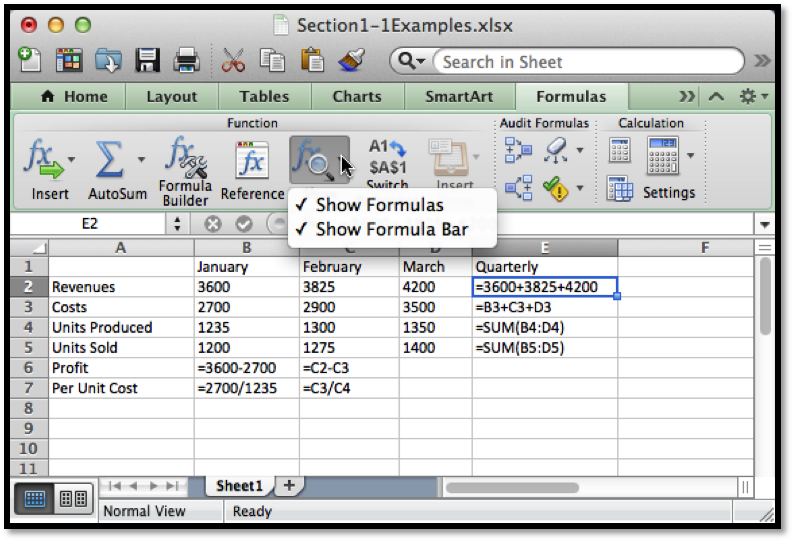
\includegraphics[width=1\linewidth]{images/sec1-3-2ShowFormulas.png}
\end{sbspanel}%
\end{sidebyside}%
\par
\hypertarget{p-239}{}%
If we unselect \terminology{Show Formulas}, we see the values that Excel computes.%
\begin{sidebyside}{1}{0.1}{0.1}{0}%
\begin{sbspanel}{0.8}%
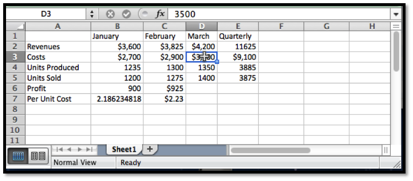
\includegraphics[width=1\linewidth]{images/sec1-3-3UnshowFormulas.png}
\end{sbspanel}%
\end{sidebyside}%
\par
\hypertarget{p-240}{}%
We want to finish our assignment by computing the Profit and Per Unit Costs for March and for the Quarter.  However, we would prefer not to type any more formulas.  (Typing in four more cells is not so bad, but we can imagine being told to do this for several years of data.)  We will use a process called Quick Fill, that tells Excel to repeat the same formula, with the cell references appropriately modified.%
\par
\hypertarget{p-241}{}%
To do the quick fill, we select the cells we want copied.%
\begin{sidebyside}{1}{0.1}{0.1}{0}%
\begin{sbspanel}{0.8}%
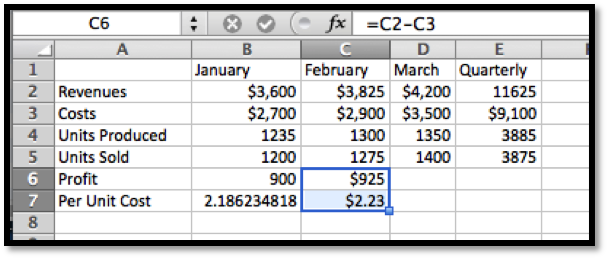
\includegraphics[width=1\linewidth]{images/sec1-3-4.png}
\end{sbspanel}%
\end{sidebyside}%
\par
\hypertarget{p-242}{}%
We can move the cursor until the cell(s) show the fill handle. This will change the symbol in the corner of the cell to a thin dark '+'.%
\begin{sidebyside}{1}{0.4}{0.4}{0}%
\begin{sbspanel}{0.2}%

\includegraphics[width=1\linewidth]{images/sec1-3-5.png}
\end{sbspanel}%
\end{sidebyside}%
\par
\hypertarget{p-243}{}%
We then drag the little blue box at the lower left corner of the box of selected cells.  Excel automatically fills in the new values.%
\begin{sidebyside}{1}{0.1}{0.1}{0}%
\begin{sbspanel}{0.8}%
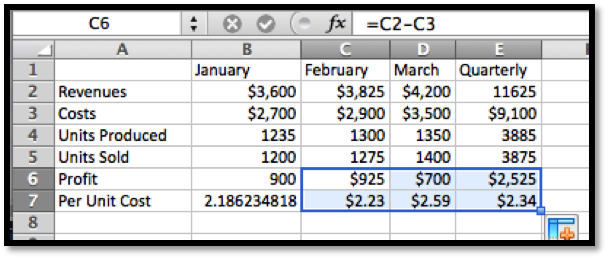
\includegraphics[width=1\linewidth]{images/sec1-3-6FebSums.png}
\end{sbspanel}%
\end{sidebyside}%
\par
\hypertarget{p-244}{}%
We look back at the formulas and see that Excel has produced formulas where cells are in the same relative position.  Profit is the value from the cell 4 rows higher minus the value of the cell three rows higher.%
\begin{sidebyside}{1}{0.1}{0.1}{0}%
\begin{sbspanel}{0.8}%
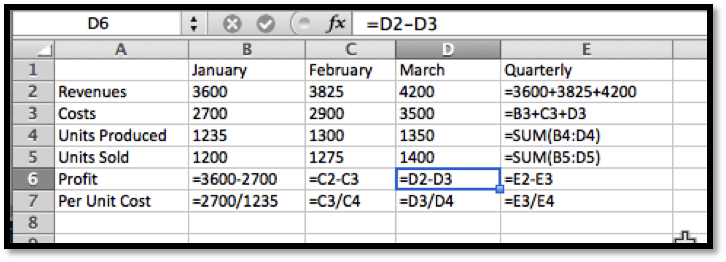
\includegraphics[width=1\linewidth]{images/sec1-3-7MoreSums.png}
\end{sbspanel}%
\end{sidebyside}%
\par
\hypertarget{p-245}{}%
There is a last detail to fix in our report.  The quantities in profit and Per Unit Cost are in money, so we want them formatted correctly.  (They should start with a dollar sign, have a decimal point, and stop at two decimal places or cents.)  We do this by selecting the cells and then formatting the cells as currency.%
\begin{sidebyside}{1}{0.1}{0.1}{0}%
\begin{sbspanel}{0.8}%
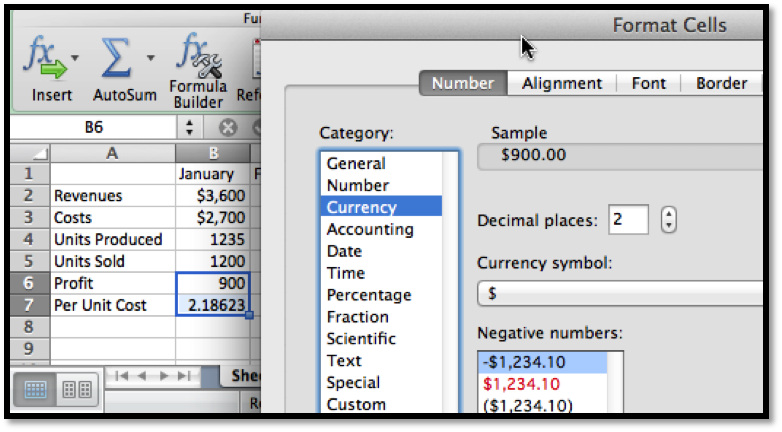
\includegraphics[width=1\linewidth]{images/sec1-3-8.png}
\end{sbspanel}%
\end{sidebyside}%
\par
\hypertarget{p-246}{}%
If we use the quick fill on a pair of numbers, Excel produces an arithmetic sequence.  A pair of cells containing 1 then 4 becomes the start of a sequence 1, 4, 7, 10,  … .%
\par
\hypertarget{p-247}{}%
\terminology{Absolute and Relative Cell References}%
\par
\hypertarget{p-248}{}%
One of the reasons that spreadsheets are so useful for doing mathematics in a business setting is that businesses often do a relatively simple computation for a large number of cases.  That means we should pay attention to formulas with cell references and the process of copying a formula from one case to another.  In the example above, all of the values change from one month to the next.  It is not hard to imagine a calculation where some values remain the same for many cases.  Thus we want to look at the idea of absolute and relative cell references.  This is a very important topic and an Excel feature we will be using for the rest of the term.%
\par
\hypertarget{p-249}{}%
Consider the following example: Your rich uncle Fred decided to give you 10 shares of Google stock (GOOG) on January first 2009, with the option of receiving instead the same value in either Microsoft (MSFT) or Apple stock (AAPL). You would like to see the monthly change in value of the portfolios over a three-year period.%
\par
\hypertarget{p-250}{}%
We start by going to finance.yahoo.com and collecting the monthly prices of the stocks, downloading the answers into a spreadsheet.  When we look up historical prices from yahoo, we are interested in the adjusted closing price.  (They adjust the price to account care of splits and dividends.)  That produces a spreadsheet like the one below.%
\begin{sidebyside}{1}{0.1}{0.1}{0}%
\begin{sbspanel}{0.8}%
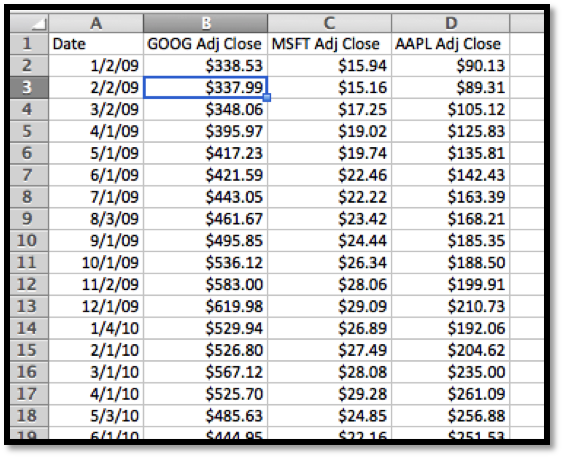
\includegraphics[width=1\linewidth]{images/sec1-3-9SharePrices.png}
\end{sbspanel}%
\end{sidebyside}%
\par
\hypertarget{p-251}{}%
Next we want to compute the number of shares for each stock.  This is 10 times the closing price of Google divided by the closing price of the stock we selected.%
\begin{sidebyside}{1}{0.1}{0.1}{0}%
\begin{sbspanel}{0.8}%
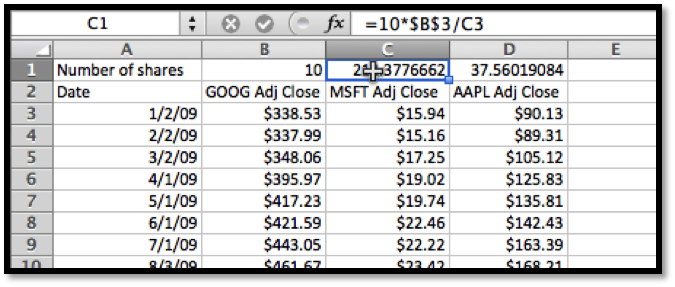
\includegraphics[width=1\linewidth]{images/sec1-3-10ShareAjustments.png}
\end{sbspanel}%
\end{sidebyside}%
\par
\hypertarget{p-252}{}%
In the formula for the number of shares of MSFT, we used \textdollar{}B\textdollar{}3 for the initial price of GOOG.  This is an absolute cell reference.  When we copy the formula from cell C1 to cell D1, the new formula is =10\textasteriskcentered{}\textdollar{}B\textdollar{}3\slash{}D3.  This formula in cell D1 asks for 10 times the value in cell B3, divided by the value in the 2 rows below the cell of the formula.%
\begin{assemblage}{}{assemblage-8}%
\hypertarget{p-253}{}%
\terminology{Absolute references} refer to a particular column and\slash{}or row.  The dollar sign '\textdollar{}' is used to fix the reference.%
\par
\hypertarget{p-254}{}%
\terminology{Relative references} refer to the cell the same distance away from the cell containing the formula.%
\end{assemblage}
\hypertarget{p-255}{}%
We continue our example by computing the change in value of our GOOG portfolio in the first month.  That will be the share price at the beginning of the next month minus the share price at the beginning of the month, times the number of shares.  For January 2009, for GOOG this becomes =(B4-B3)\textasteriskcentered{}B\textdollar{}1.%
\begin{sidebyside}{1}{0.05}{0.05}{0}%
\begin{sbspanel}{0.9}%
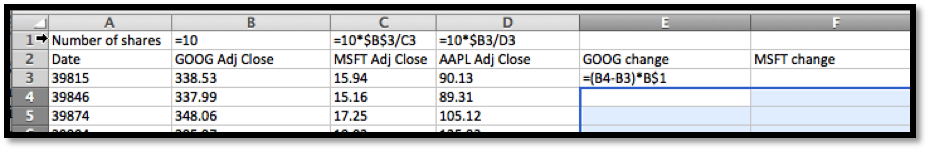
\includegraphics[width=1\linewidth]{images/sec1-3-11.png}
\end{sbspanel}%
\end{sidebyside}%
\par
\hypertarget{p-256}{}%
Since we have properly used relative and absolute references, we can now copy this formula to complete the chart, and Excel will modify the formula appropriately.%
\begin{sidebyside}{1}{0.1}{0.1}{0}%
\begin{sbspanel}{0.8}%
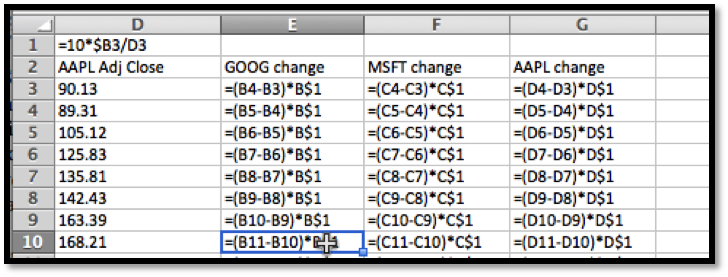
\includegraphics[width=1\linewidth]{images/sec1-3-12.png}
\end{sbspanel}%
\end{sidebyside}%
\par
\hypertarget{p-257}{}%
We note that the rows and columns can be independently made absolute or relative.  Thus if we are looking at a formula in cell A1, and see a reference to B2 it means the cell one below and to the right of the location of the formula.  If we see \textdollar{}B2 it means the cell in column B that is one row down from the formula.  If we see B\textdollar{}2 it means the cell in row two that is one column to the right of the formula.%
\par
\hypertarget{p-258}{}%
When we convert back to see the values, we see that an original investment of \textdollar{}3,385.30 would have made a profit of \textdollar{}3,073.70 in GOOG stock, \textdollar{}2,128.02 in MSFT stock and \textdollar{}11,826.60 in AAPL stock.  Once again we use the SUM function and a cell range to add the values in the column.  We also use the split screen icons in the scroll bars to be able to see the correct rows and columns.%
\begin{sidebyside}{1}{0.1}{0.1}{0}%
\begin{sbspanel}{0.8}%
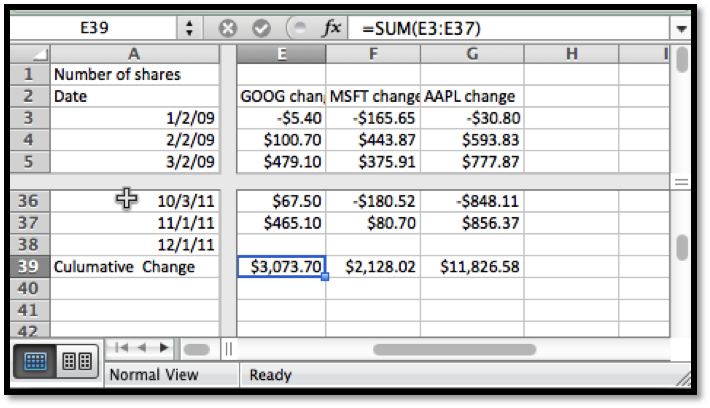
\includegraphics[width=1\linewidth]{images/sec1-3-13.png}
\end{sbspanel}%
\end{sidebyside}%
\par
\hypertarget{p-259}{}%
\terminology{Note}: Excel can also make references across multiple pages of a workbook, but we will not need that capability for htis course.%
\par
\hypertarget{p-260}{}%
\terminology{Named Cell References}%
\par
\hypertarget{p-261}{}%
An alternative to using absolute references in formulas is to name the cells.%
\begin{assemblage}{}{assemblage-9}%
\hypertarget{p-262}{}%
By default, Excel names each cell by its row and column.  We can use the name cell in the upper left corner of the Excel sheet to change the name from the letter\slash{}number format into a descriptive name.%
\end{assemblage}
\hypertarget{p-263}{}%
The more descriptive name can be useful when constructing and documenting the process we are using for our computations.  Consider the previous example with the rich uncle.  In cells B1, C1, and D1, we had the number of shares of Google, Microsoft, and Apple we could have had in the portfolio.  Better names for those cells would then be SharesGOOG, SharesMSFT, and SharesAAPL.  We can name a cell by editing the name box at the left side of the formula bar.%
\begin{sidebyside}{1}{0.3}{0.3}{0}%
\begin{sbspanel}{0.4}%
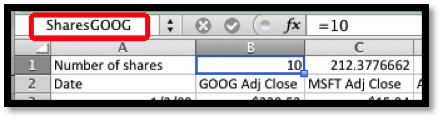
\includegraphics[width=1\linewidth]{images/sec1-3-14.png}
\end{sbspanel}%
\end{sidebyside}%
\par
\hypertarget{p-264}{}%
We can then use the names in formulas.  In general, the formulas with nicely named variables are easier to read.%
\begin{sidebyside}{1}{0.1}{0.1}{0}%
\begin{sbspanel}{0.8}%
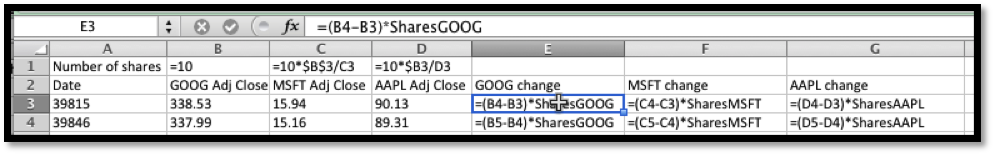
\includegraphics[width=1\linewidth]{images/sec1-3-15.png}
\end{sbspanel}%
\end{sidebyside}%
\par
\hypertarget{p-265}{}%
\terminology{Getting Help}%
\par
\hypertarget{p-266}{}%
One of the ways that doing mathematics with a program like Excel differs from working with a calculator is that computer programs have help features.  It is worthwhile pointing out two that come with Excel.  We illustrate both with the SUM function we have used a number of times.%
\par
\hypertarget{p-267}{}%
When we call Help from the top menu, we are given a pop up window for Excel Help.  It has a number of topics listed by default.  It also has a bar for searching topics.%
\begin{sidebyside}{1}{0.1}{0.1}{0}%
\begin{sbspanel}{0.8}%

\includegraphics[width=1\linewidth]{images/sec1-3-16.png}
\end{sbspanel}%
\end{sidebyside}%
\par
\hypertarget{p-268}{}%
We type the name of the command we are looking for and we are given a page of help for that command.%
\begin{sidebyside}{1}{0.1}{0.1}{0}%
\begin{sbspanel}{0.8}%
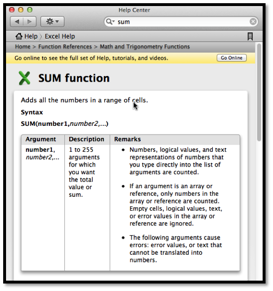
\includegraphics[width=1\linewidth]{images/sec1-3-17.png}
\end{sbspanel}%
\end{sidebyside}%
\par
\hypertarget{p-269}{}%
A second kind of help is the formula builder from the formula ribbon.  It gives a more concise help when you do not remember the exact syntax of a command.%
\begin{sidebyside}{1}{0.1}{0.1}{0}%
\begin{sbspanel}{0.8}%
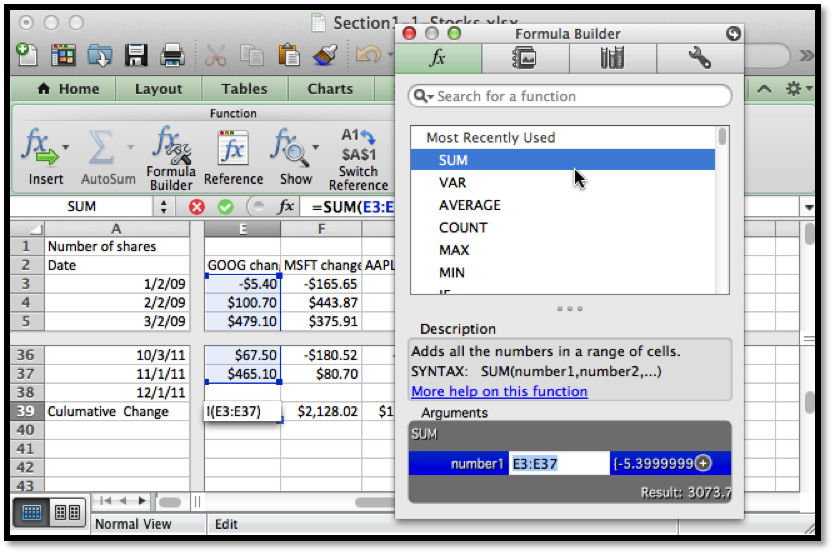
\includegraphics[width=1\linewidth]{images/sec1-3-18.png}
\end{sbspanel}%
\end{sidebyside}%
\par
\hypertarget{p-270}{}%
A third source of help is simply to do a web search for excel help.  To find how to do a computation with an exponential functions you can search for “Excel formulas exponential.”%
\par
\hypertarget{p-271}{}%
\terminology{Other Details}%
\par
\hypertarget{p-272}{}%
Excel is a rich and complex tool.  We will be looking at more features as we go through the course.  There are several that are worth pointing out explicitly at this point.%
\leavevmode%
\begin{itemize}[label=\textbullet]
\item{}\hypertarget{p-273}{}%
For ordinary arithmetic, Excel uses the standard symbols of +, -, \textasteriskcentered{}, \slash{}, and \textasciicircum{} for plus, minus, times, divided by, and raising to a power.%
\item{}\hypertarget{p-274}{}%
We can also use the SUM, PRODUCT, QUOTIENT, and POWER commands for ordinary arithmetic.%
\item{}\hypertarget{p-275}{}%
The order of operations used by Excel differs from the traditional order of operations when it comes to taking powers of negative numbers.  The problem is illustrated in evaluating  \(-3^2\), which has a negative sign and an exponentiation. In all math classes you have taken this is interpreted as \(-(3^2)\) or \(-9\), with exponentiation done first.  In Excel, this is interpreted as \((-3)^2\) or 9, with negation done first.  When in doubt, use parenthesis to make the order of operations explicit.%
\item{}\hypertarget{p-276}{}%
Excel also has the other mathematical functions you have used before.  The functions for square root, log base 10, log base e, and e to the power of, are respectively, SQRT, LOG, LN, and EXP.%
\item{}\hypertarget{p-277}{}%
The value of e is represented by EXP(1).%
\item{}\hypertarget{p-278}{}%
Excel has a number of very useful operations on collections of numbers.  We start with easy ones where the name is self explanatory, like SUM, AVERAGE, COUNT, MIN, and MAX.%
\end{itemize}
%
%
\typeout{************************************************}
\typeout{Exercises 1.3 Exercises Introduction to Excel Spreadsheets}
\typeout{************************************************}
%
\begin{exercises-subsection-numberless}{Exercises Introduction to Excel Spreadsheets}{}{Exercises Introduction to Excel Spreadsheets}{}{}{exercises-set-sec-1-3}
\begin{divisionexercise}{1}{}{}{exercise-43}%
\hypertarget{p-279}{}%
Produce a spreadsheet where the first 100 rows are used.  The cell in row n and column A should have value n.  The cell in row n and column B should have value 2\textasteriskcentered{}n.  You should be able to do this by typing in the value of 4 cells and using quick fill.%
\par\smallskip%
\noindent\textbf{Solution}.\hypertarget{solution-22}{}\quad%
\hypertarget{p-280}{}%
The formulas entered should look like this:%
\begin{sidebyside}{1}{0.1}{0.1}{0}%
\begin{sbspanel}{0.8}%
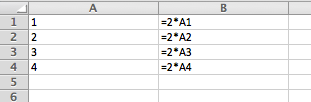
\includegraphics[width=1\linewidth]{images/sec1-3-sol1a.png}
\end{sbspanel}%
\end{sidebyside}%
\par
\hypertarget{p-281}{}%
Once we quickfill and have the regular view (not showing the formulas)%
\begin{sidebyside}{1}{0.25}{0.25}{0}%
\begin{sbspanel}{0.5}%
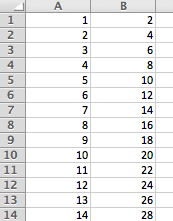
\includegraphics[width=1\linewidth]{images/sec1-3-sol1b.png}
\end{sbspanel}%
\end{sidebyside}%
\leavevmode%
\begin{itemize}[label=\textbullet]
\item{}\hypertarget{p-282}{}%
The actual spreadsheet has 100 rows.%
\item{}\hypertarget{p-283}{}%
Note that there is a small window that shows how far the quickfill has gone.%
\item{}\hypertarget{p-284}{}%
If you want to check the formulas used you go to the “Formula” menu and choose “Show formulas”. This feature is good for debugging any problem that may happen.%
\end{itemize}
\end{divisionexercise}%
\begin{divisionexercise}{2}{}{}{exercise-44}%
\hypertarget{p-285}{}%
Produce a spreadsheet where the first 100 rows are used.  Column A should contain the first 100 odd numbers.  Column B should contain multiples of 7 starting with 21.%
\end{divisionexercise}%
\begin{divisionexercise}{3}{}{}{exercise-45}%
\hypertarget{p-286}{}%
Start with the worksheet given.  Complete the worksheet in such a way that if the values of x, y, and z are changed, the other values are automatically recomputed. \leavevmode%
\begin{sidebyside}{1}{0.1}{0.1}{0}%
\begin{sbspanel}{0.8}%
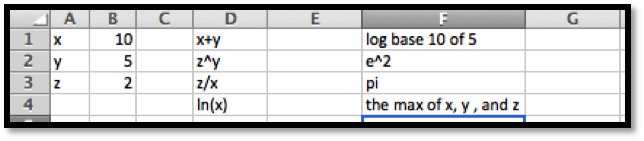
\includegraphics[width=1\linewidth]{images/sec1-3-e1.png}
\end{sbspanel}%
\end{sidebyside}%
%
\par\smallskip%
\noindent\textbf{Solution}.\hypertarget{solution-23}{}\quad%
\hypertarget{p-287}{}%
We do not need to use absolute references in this case, but when we are computing something involving the \(x\), \(y\) and \(z\) values we should refer to cells B1, B2, and B3 respectively.%
\begin{sidebyside}{1}{0.1}{0.1}{0}%
\begin{sbspanel}{0.8}%
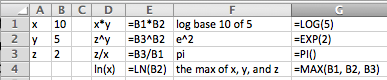
\includegraphics[width=1\linewidth]{images/sec1-3-sol3b.png}
\end{sbspanel}%
\end{sidebyside}%
\par
\hypertarget{p-288}{}%
The spreadsheet should have entries as shown above.%
\end{divisionexercise}%
\begin{divisionexercise}{4}{}{}{exercise-46}%
\hypertarget{p-289}{}%
Produce a spreadsheet where the first 101 rows are used.  Row 1 should be used for labels. Column A should contain integers from 1 to 100.  Columns B through F should contain the squares, cubes, square roots, logs base 10 and natural logs of the entries in columns A.%
\end{divisionexercise}%
\begin{divisionexercise}{5}{}{}{exercise-47}%
\hypertarget{p-290}{}%
Start with the spreadsheet section below. \leavevmode%
\begin{sidebyside}{1}{0.2}{0.2}{0}%
\begin{sbspanel}{0.6}%
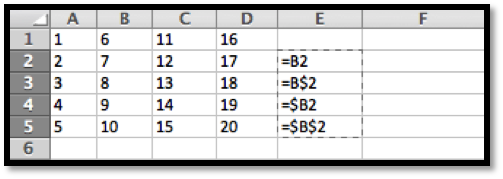
\includegraphics[width=1\linewidth]{images/sec1-3-e2.png}
\end{sbspanel}%
\end{sidebyside}%
 If column E is copied and pasted into column G, give both the formula and value for each non-empty cell in column G.%
\par\smallskip%
\noindent\textbf{Solution}.\hypertarget{solution-24}{}\quad%
\hypertarget{p-291}{}%
Any entry that is absolute (with a \textdollar{}) will be fixed. The relative references (without the \textdollar{}) will change all the Bs to Ds because we moved over 2 columns.%
\par
\hypertarget{p-292}{}%
Formulas \leavevmode%
\begin{sidebyside}{1}{0.1}{0.1}{0}%
\begin{sbspanel}{0.8}%
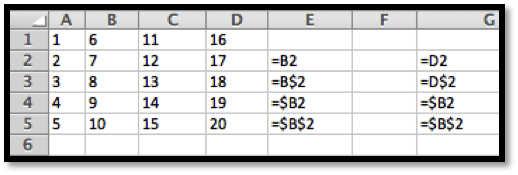
\includegraphics[width=1\linewidth]{images/sec1-3-sol5a.png}
\end{sbspanel}%
\end{sidebyside}%
%
\par
\hypertarget{p-293}{}%
Entries \leavevmode%
\begin{sidebyside}{1}{0.1}{0.1}{0}%
\begin{sbspanel}{0.8}%
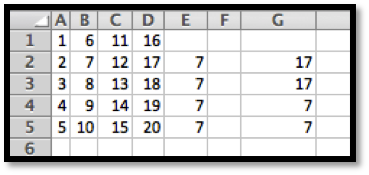
\includegraphics[width=1\linewidth]{images/sec1-3-sol5b.png}
\end{sbspanel}%
\end{sidebyside}%
%
\end{divisionexercise}%
\begin{divisionexercise}{6}{}{}{exercise-48}%
\hypertarget{p-294}{}%
We would like to really understand what happens when we use quick fill.%
\leavevmode%
\begin{enumerate}[label=(\Alph*)]
\item\hypertarget{li-96}{}\hypertarget{p-295}{}%
Let's consider the entries =A1, =\textdollar{}A1, =A\textdollar{}1, and =\textdollar{}A\textdollar{}1 in row 2.  Do quick fill below to fill in 3 more rows and see what happens. Clearly in the first row these cells all now point to cell A1 and the value returned is 1. After the first row we get a mixture of values. Why?%
\begin{sidebyside}{1}{0.1}{0.1}{0}%
\begin{sbspanel}{0.8}%
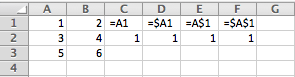
\includegraphics[width=1\linewidth]{images/sec1-3-e3.png}
\end{sbspanel}%
\end{sidebyside}%
\item\hypertarget{li-97}{}\hypertarget{p-296}{}%
Next, we can set up the values in column D. Do quick fill to fill in the 3 columns to the right? Explain the pattern of values we see. \leavevmode%
\begin{sidebyside}{1}{0.1}{0.1}{0}%
\begin{sbspanel}{0.8}%
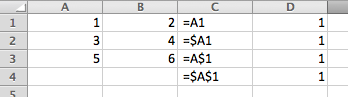
\includegraphics[width=1\linewidth]{images/sec1-3-e4.png}
\end{sbspanel}%
\end{sidebyside}%
%
\end{enumerate}
\end{divisionexercise}%
\begin{divisionexercise}{7}{}{}{exercise-49}%
\hypertarget{p-297}{}%
Complete the spreadsheet section below so that columns A through C are complete for numbers 1 to 100.  (The value for a should be a random number generated by the formula in cell E1.) \leavevmode%
\begin{sidebyside}{1}{0.2}{0.2}{0}%
\begin{sbspanel}{0.6}%
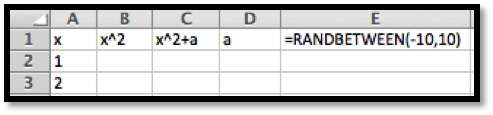
\includegraphics[width=1\linewidth]{images/sec1-3-e5.png}
\end{sbspanel}%
\end{sidebyside}%
%
\par\smallskip%
\noindent\textbf{Solution}.\hypertarget{solution-25}{}\quad%
\hypertarget{p-298}{}%
The random number will differ from person to person, but the Excel entries are as follows. Note that we need to use an absolute reference for the value of a !%
\par
\hypertarget{p-299}{}%
Formulas \leavevmode%
\begin{sidebyside}{1}{0.1}{0.1}{0}%
\begin{sbspanel}{0.8}%
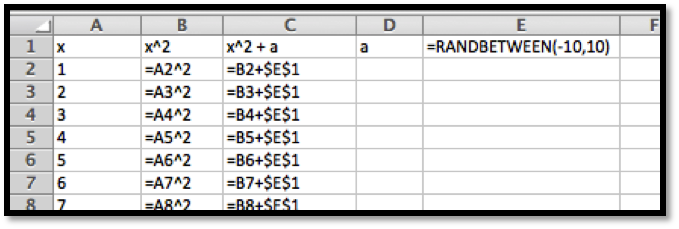
\includegraphics[width=1\linewidth]{images/sec1-3-sol7a.png}
\end{sbspanel}%
\end{sidebyside}%
%
\par
\hypertarget{p-300}{}%
The entry in C2 could also have been given as =A2\textasciicircum{}2+\textdollar{}E\textdollar{}1.%
\par
\hypertarget{p-301}{}%
Just E\textdollar{}1 will work as well. We are filling down so we really need to fix the row in this case.%
\par
\hypertarget{p-302}{}%
In this version the random number settled on -6 (yours is likely different) and the first part of the table looks as follows. The actual answer has all 100 rows completed. \leavevmode%
\begin{sidebyside}{1}{0.1}{0.1}{0}%
\begin{sbspanel}{0.8}%
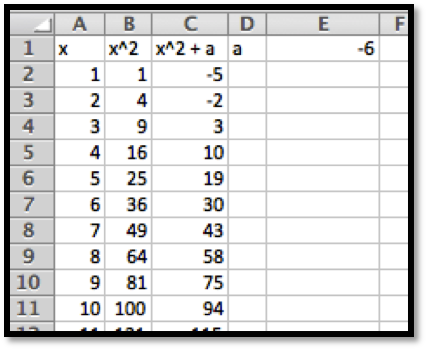
\includegraphics[width=1\linewidth]{images/sec1-3-sol7b.png}
\end{sbspanel}%
\end{sidebyside}%
%
\end{divisionexercise}%
\begin{divisionexercise}{8}{}{}{exercise-50}%
\hypertarget{p-303}{}%
Using the help functions to check syntax, write a formula for cell B2, that looks at the value for cell A2, and if it is negative, returns the square of it, and if positive returns its square root.%
\end{divisionexercise}%
\begin{divisionexercise}{9}{}{}{exercise-51}%
\hypertarget{p-304}{}%
Using your favorite source on the web create a spreadsheet that has the closing price of your favorite stock on the first day of the month for the past 5 years.  Compute the change in adjusted stock price for each month and identify which month had the greatest increase. (\href{http://finance.yahoo.com/}{http:\slash{}\slash{}finance.yahoo.com\slash{}}) is one source for such data.)%
\par\smallskip%
\noindent\textbf{Solution}.\hypertarget{solution-26}{}\quad%
\hypertarget{p-305}{}%
For example if we type in Coca-Cola we get to ``The Coca-Cola Company (KO)''%
\par
\hypertarget{p-306}{}%
From the menu on the left choose “Historical Prices” and pull the monthly data from the past 5 years. Then scroll down and download to spreadsheet.%
\par
\hypertarget{p-307}{}%
Using the Adjusted close we compute the change: \leavevmode%
\begin{sidebyside}{1}{0.1}{0.1}{0}%
\begin{sbspanel}{0.8}%
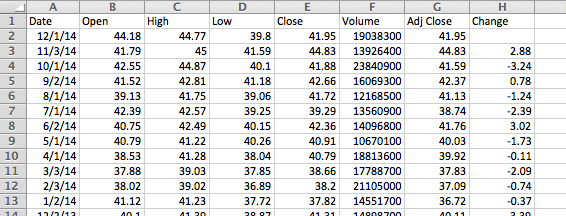
\includegraphics[width=1\linewidth]{images/sec1-3-sol9a.png}
\end{sbspanel}%
\end{sidebyside}%
%
\par
\hypertarget{p-308}{}%
The above partial table shows what the table should look like.%
\par
\hypertarget{p-309}{}%
Using the MAX function for this data the biggest change is \textdollar{}3.39.%
\par
\hypertarget{p-310}{}%
Finding the month can be done by inspection as this point (there are more sophisticated ways to do this, but that requires rather advanced Excel commands). In this instance the greatest change took place in December 2013.%
\end{divisionexercise}%
\begin{divisionexercise}{10}{}{}{exercise-52}%
\hypertarget{p-311}{}%
Using your favorite source on the web create a spreadsheet that has the closing price of your favorite stock on the first day of the month for the past 5 years.  Compute the percentage change in adjusted stock price for each month and identify which month had the greatest increase.%
\end{divisionexercise}%
\begin{divisionexercise}{11}{}{}{exercise-53}%
\hypertarget{p-312}{}%
Create a spreadsheet showing the Consumer Price Index by month from 1930-2010.  (Good sources are \href{http://inflationdata.com/}{http:\slash{}\slash{}inflationdata.com\slash{}} and \href{http://www.bls.gov/cpi/}{http:\slash{}\slash{}www.bls.gov\slash{}cpi\slash{}} at the Bureau of Labor Statistics.)  Compute the percentage change between January and July for each year.  Which year had the greatest percentage change in the first half of the year?%
\end{divisionexercise}%
\end{exercises-subsection-numberless}
\end{sectionptx}
%
%
\typeout{************************************************}
\typeout{Section 1.4 Graphing functions with Excel}
\typeout{************************************************}
%
\begin{sectionptx}{Graphing functions with Excel}{}{Graphing functions with Excel}{}{}{sec-1-4-GraphingFunctionsExcel}
\hypertarget{p-313}{}%
\href{./Examples/Section-1-4-Examples.xlsx}{Link to worksheets used in this section}%
\par
\hypertarget{p-314}{}%
One area where Excel is different from a graphing calculator is in producing the graph of a function that has been defined by a formula.  It is not difficult, but it is not as straight forward as with a calculator. It is a skill worth developing however.  When we are given a formula as part of a problem, we will want to easily see a graph of the function.%
\par
\hypertarget{p-315}{}%
We will walk through the process for producing graphs for three examples of increasing complexity.  For the first example we have a specific function and specific range in mind, say \(y=x^2-6 x\) over \(-10 \le x \le 10\).  For the second example, we would like to use parameters in the formula, for example, \(y = a x^2 + b x + c\), with specified values of a, b, and c, and have the ability to easily change the values of the parameters and see the graph.  For the third example we would also like to have the ability to change the domain, graphing over \(xLow \le x \le xHigh\), where \(xLow\) and \(xHigh\) can easily be changed.%
\begin{example}{A basic graph.}{example-5}%
\hypertarget{p-316}{}%
graphing \(y=x^2-6 x\) over \(-10 \le x \le 10\).%
\begin{sidebyside}{1}{0.1}{0.1}{0}%
\begin{sbspanel}{0.8}%
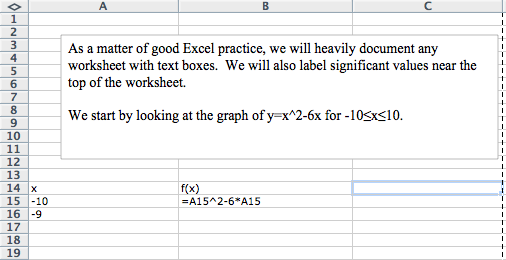
\includegraphics[width=1\linewidth]{images/sec1-4-1.png}
\end{sbspanel}%
\end{sidebyside}%
\par
\hypertarget{p-317}{}%
We start by producing a column for x and one for f(x).  In the column for x we start with values -10 and -9, so that we can complete the column with a quick fill.  Similarly, we start the f(x) columns in the first cell with the "x" replaced by the appropriate cell reference.  In this case the formula for f(x) is in cell B15 and x is in cell A15.%
\par
\hypertarget{p-318}{}%
We then use quick fill and quick copy to fill out the table.%
\begin{sidebyside}{1}{0.2}{0.2}{0}%
\begin{sbspanel}{0.6}%
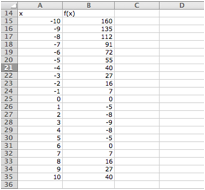
\includegraphics[width=1\linewidth]{images/sec1-4-2.png}
\end{sbspanel}%
\end{sidebyside}%
\par
\hypertarget{p-319}{}%
With the values of the cells filled in we highlight the cells we want to graph (A14 through B35) and add a scatter plot for the highlighted values.%
\begin{sidebyside}{1}{0.1}{0.1}{0}%
\begin{sbspanel}{0.8}%
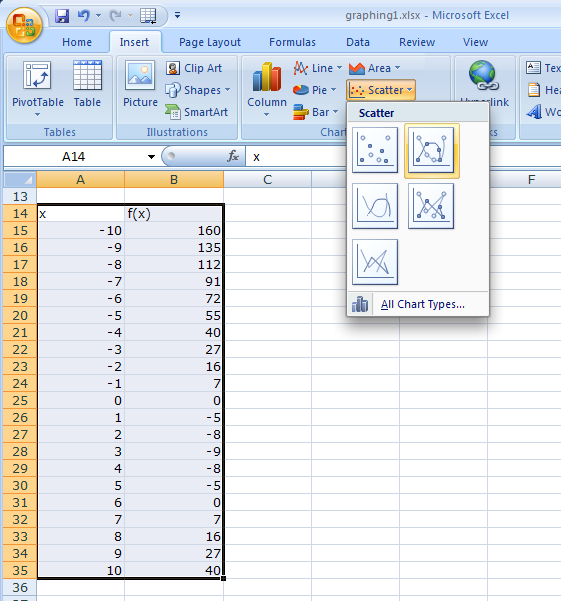
\includegraphics[width=1\linewidth]{images/sec1-4-3.png}
\end{sbspanel}%
\end{sidebyside}%
\par
\hypertarget{p-320}{}%
(The location of the scatterplot will be a bit different with Macs.  The scatterplot is in the Charts ribbon, under other, on Macs.)  This gives the desired graph.%
\begin{sidebyside}{1}{0.1}{0.1}{0}%
\begin{sbspanel}{0.8}%
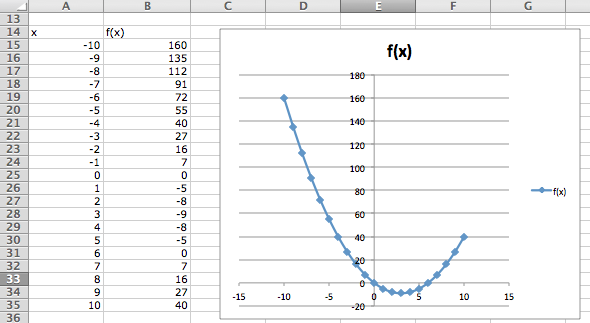
\includegraphics[width=1\linewidth]{images/sec1-4-4.png}
\end{sbspanel}%
\end{sidebyside}%
\end{example}
\begin{example}{A graph with parameters.}{example-6}%
\hypertarget{p-321}{}%
– graphing \(y=x^2-6 x\) as an example of \(y = a x^2 + b x + c\) over the domain \(-10 \le x \le 10\).%
\par
\hypertarget{p-322}{}%
For the second example, we want the same graph, but we want the ability to easily convert the graph of our first quadratic into a different quadratic function.  The solution is to consider a, b, and c to be parameters that we can change.%
\par
\hypertarget{p-323}{}%
Toward the top of the worksheet, we put the labels \(a\), \(b\), and \(c\), and give values for those parameters.  In this case the values of \(a\), \(b\), and \(c\) are in cells B9, B10, and B11 respectively.%
\par
\hypertarget{p-324}{}%
Now we set up the problem in the same way we did above except that we are using absolute references for \(a\), \(b\), and \(c\), and relative references for \(x\).%
\begin{sidebyside}{1}{0.1}{0.1}{0}%
\begin{sbspanel}{0.8}%
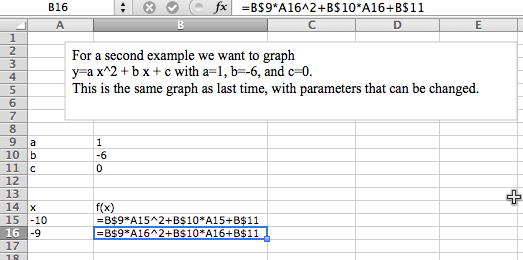
\includegraphics[width=1\linewidth]{images/sec1-4-5.png}
\end{sbspanel}%
\end{sidebyside}%
\par
\hypertarget{p-325}{}%
Now, we once again do a quick fill to complete the table, and then add a scatterplot.%
\begin{sidebyside}{1}{0.1}{0.1}{0}%
\begin{sbspanel}{0.8}%
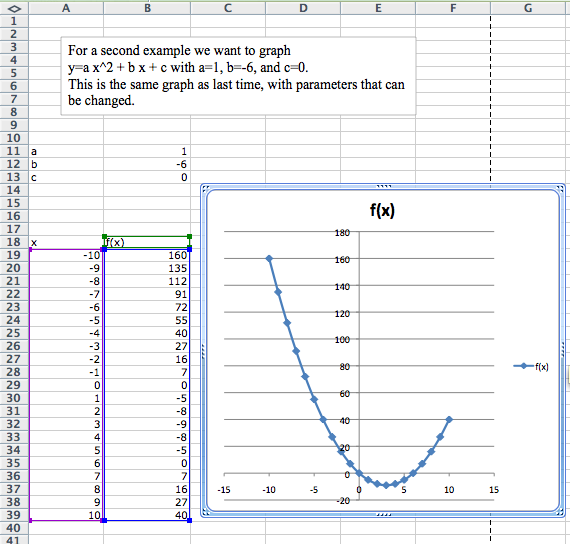
\includegraphics[width=1\linewidth]{images/sec1-4-6.png}
\end{sbspanel}%
\end{sidebyside}%
\par
\hypertarget{p-326}{}%
The difference with this second example is that if I now want to look at the graph of \(y = -x^2 + 3 x + 10\), I simply change the values of the parameters \(a\), \(b\), and \(c\).%
\begin{sidebyside}{1}{0.1}{0.1}{0}%
\begin{sbspanel}{0.8}%
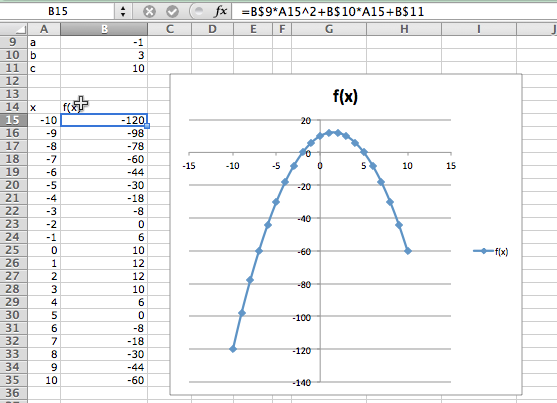
\includegraphics[width=1\linewidth]{images/sec1-4-7.png}
\end{sbspanel}%
\end{sidebyside}%
\end{example}
\begin{example}{Controlling the viewing window.}{example-7}%
\hypertarget{p-327}{}%
graphing \(y=x^2 - 6 x\) as an example of \(y = a x^2 + b x + c\) over the domain \(-10 \le x \le 10\), but with the ability to easily change the domain of the graph.%
\par
\hypertarget{p-328}{}%
Often, when we graph, we will want to change the domain of the graph.  Most easily, I may want to zoom in on a particular region to get a better view of some interesting feature.  I may want to look closely at several different regions.%
\par
\hypertarget{p-329}{}%
To do this we will again plot 21 points, but we want to have control of the starting point and the change in x between the first and second points.  First we add labels and values for x-start and x-step.  Then we need a bit of care in defining the values of x.  The first value of x (cell A18) is the value of x-start.  Every other value of x is defined as the previous value of x plus the value of x-step.%
\begin{sidebyside}{1}{0.1}{0.1}{0}%
\begin{sbspanel}{0.8}%
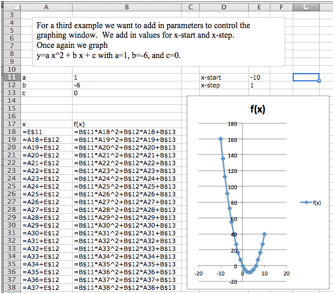
\includegraphics[width=1\linewidth]{images/sec1-4-8.png}
\end{sbspanel}%
\end{sidebyside}%
\par
\hypertarget{p-330}{}%
In this case I want a better look at the vertex of the parabola.  I decide I want to see the graph for \(0 \le x \le 5\).  My value for x-start is 0.  My value for x-step is one twentieth of the distance from 0 to 5, or \((5-0)/20 = 0.25\).  I plug those values in and see the graph.%
\begin{sidebyside}{1}{0.1}{0.1}{0}%
\begin{sbspanel}{0.8}%
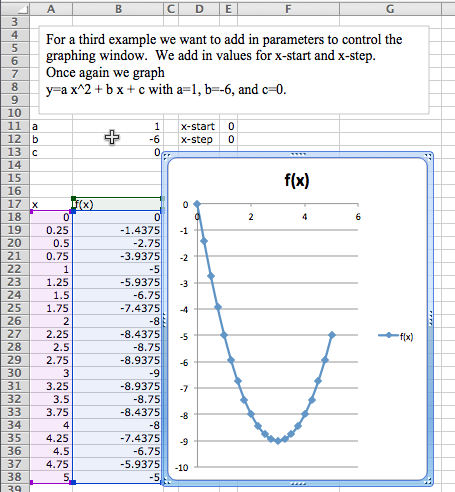
\includegraphics[width=1\linewidth]{images/sec1-4-9.png}
\end{sbspanel}%
\end{sidebyside}%
\end{example}
\hypertarget{p-331}{}%
\terminology{Graphing more than one function}%
\par
\hypertarget{p-332}{}%
We would also like to put two or more graphs together.  For our examples, we will want to use the functions \(f(x) = x – 3\), \(g(x) = (x^2 – x)/10\), and \(h(x) = x^3 – x\).  We start by using the procedure given above to make a chart of values for the three functions.%
\begin{sidebyside}{1}{0.2}{0.2}{0}%
\begin{sbspanel}{0.6}%
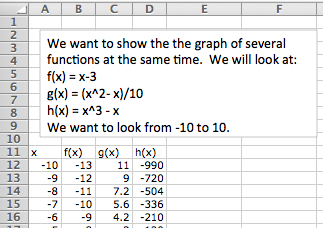
\includegraphics[width=1\linewidth]{images/sec1-4-10.png}
\end{sbspanel}%
\end{sidebyside}%
\par
\hypertarget{p-333}{}%
We then simply select the cells for \(x\) and the functions we want graphed together and produce a scatterplot as before.  (To graph \(g(x)\) and \(h(x)\) together, we want to select the columns for \(x\), \(g(x)\), and \(h(x)\).)%
\begin{sidebyside}{1}{0.1}{0.1}{0}%
\begin{sbspanel}{0.8}%
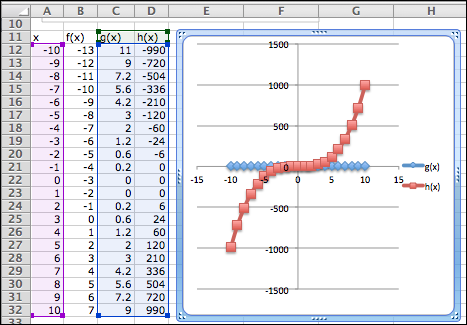
\includegraphics[width=1\linewidth]{images/sec1-4-11.png}
\end{sbspanel}%
\end{sidebyside}%
\par
\hypertarget{p-334}{}%
One problem with the graph of \(g(x)\) and \(h(x)\) together is that the functions have different orders of magnitude, so we do not see that \(y = g(x)\) is a parabola.  One remedy is to use a secondary axis for the graph of \(h(x)\).  (Simply double click on one of the points for \(h(x)\), and select secondary axis from the axes tab.)%
\begin{sidebyside}{1}{0.1}{0.1}{0}%
\begin{sbspanel}{0.8}%
\includegraphics[width=1\linewidth]{images/sec1-4-12.png}
\end{sbspanel}%
\end{sidebyside}%
\par
\hypertarget{p-335}{}%
\terminology{Formatting a chart}%
\par
\hypertarget{p-336}{}%
Excel has a lot of ways to add formatting to a graph or chart, many more than we want to be concerned with at this point.  We simply point out a few and leave it to the reader to explore how this should be used for a good visual presentation.  If you click once on the chart to select it, the Chart tab in the home ribbon, adds sub-tabs for layout and format.  With Chart Title, you can add a title to the chart, then edit it.  The Axes icon allows you to add titles for the axes.  If you select a data point form \(g(x)\), you can then use the Data Labels icon to add values next to the points.  The chart with these annotations is given below.  The rule of thumb to follow is to add enough annotations for a reader to be able to easily understand what is happening in the chart.%
\begin{sidebyside}{1}{0.1}{0.1}{0}%
\begin{sbspanel}{0.8}%
\includegraphics[width=1\linewidth]{images/sec1-4-13.png}
\end{sbspanel}%
\end{sidebyside}%
\par
\hypertarget{p-337}{}%
It is also worthwhile to note that you can manually set the y-range of a graph by double clicking on the axis and setting the values.  This is particularly useful of the function has a vertical asymptote.%
\par
\hypertarget{p-338}{}%
\terminology{Online graphing tools: Wolfram Alpha}%
\par
\hypertarget{p-339}{}%
Throughout this book, we are limiting ourselves to mathematical tools that the student can reasonably expect to find in a generic work environment.  That is one of the reasons for focusing on using spreadsheets and Excel.  A second reason is that we will spend a significant amount of time on functions defined by data points, where we then try to construct a formula.  However when we are starting with a formula, there are easier ways to produce a graph.  The simplest is to use the free website, Wolfram Alpha.  For example to obtain a graph of the functions \(f(x) = x^2 – 3 x\), as \(x\) ranges from \(-5\) to \(5\), we simply type “plot x\textasciicircum{}2 – 3 x for x from -5 to 5” and obtain:%
\begin{sidebyside}{1}{0.1}{0.1}{0}%
\begin{sbspanel}{0.8}%
\includegraphics[width=1\linewidth]{images/sec1-4-14.png}
\end{sbspanel}%
\end{sidebyside}%
\par
\hypertarget{p-340}{}%
We will return to Wolfram Alpha from time to time, when we have nice formulas to manipulate.%
%
%
\typeout{************************************************}
\typeout{Exercises 1.4 Exercises 1.4 Graphing functions with Excel}
\typeout{************************************************}
%
\begin{exercises-subsection-numberless}{Exercises 1.4 Graphing functions with Excel}{}{Exercises 1.4 Graphing functions with Excel}{}{}{exercises-set-sec-1-4}
\begin{divisionexercise}{1}{}{}{exercise-54}%
\hypertarget{p-341}{}%
Produce a worksheet that with a graph of the function \(f(x) = x^2 - 5 x\), with \(x\) going from -10 to 10 by 1.%
\par\smallskip%
\noindent\textbf{Solution}.\hypertarget{solution-27}{}\quad%
\hypertarget{p-342}{}%
The entry in cell B2 is \mono{=A2\textasciicircum{}2-5*A2}; remember to use quickfill to complete the table%
\begin{sidebyside}{1}{0.1}{0.1}{0}%
\begin{sbspanel}{0.8}%
\includegraphics[width=1\linewidth]{images/sec1-4-sol1a.png}
\end{sbspanel}%
\end{sidebyside}%
\end{divisionexercise}%
\begin{divisionexercise}{2}{}{}{exercise-55}%
\hypertarget{p-343}{}%
Produce a worksheet that with a graph of the function \(g(x) = (x^2 - 5 x)/(x^2 + 7 x + 10)\), with \(x\) going from -10 to 10 by 1.  Explain why the graph is inaccurate.  (Pay attention to places where there should be asymptotes.)%
\par
\hypertarget{p-344}{}%
2\textasteriskcentered{} - Extra credit) – Fix the graph from problem 2 by adjusting the set of x-values used.%
\end{divisionexercise}%
\begin{divisionexercise}{3}{}{}{exercise-56}%
\hypertarget{p-345}{}%
Produce a worksheet with a graph of \(h(x) = x^3 + a x^2 + b x + c\) for \(x\) from -10 to 10, where the values of \(a\), \(b\), and \(c\) can be changed and the graph will update automatically.  For initial values, use \(a = -2\), \(b = 1\), and \(c = -11\).%
\par\smallskip%
\noindent\textbf{Solution}.\hypertarget{solution-28}{}\quad%
\hypertarget{p-346}{}%
The entry in B5 should be \mono{=A5\textasciicircum{}3+\$B\$1*A5\textasciicircum{}2+\$B\$2*A5+\$B\$3}. Note that the references to \(a\), \(b\) and \(c\) are absolute references.%
\begin{sidebyside}{1}{0}{0}{0}%
\begin{sbspanel}{1}%
\includegraphics[width=1\linewidth]{images/sec1-4-sol3a.png}
\end{sbspanel}%
\end{sidebyside}%
\end{divisionexercise}%
\begin{divisionexercise}{4}{}{}{exercise-57}%
\hypertarget{p-347}{}%
Produce a worksheet with a graph of \(k(x) = (x^2 + a x + b)/( x + c)\) for x from -10 to 10, where the values of \(a\), \(b\), and \(c\) can be changed and the graph will update automatically.  For initial values, use \(a = -5\), \(b = 2\), and \(c = -11\).%
\end{divisionexercise}%
\begin{divisionexercise}{5}{}{}{exercise-58}%
\hypertarget{p-348}{}%
Produce a worksheet with a graph of \(h(x) = x^3 -2 x^2 +  x -11\) for \(x\) going from a to b, where the values of \(a\) and \(b\) can be changed and the graph will update automatically.  For initial values, use \(a = -5\) and \(b = 5\).%
\par\smallskip%
\noindent\textbf{Solution}.\hypertarget{solution-29}{}\quad%
\hypertarget{p-349}{}%
The entries are \(a\) and \(b\), and the step size. We assume here that we are using 10 points to create a graph.%
\begin{sidebyside}{1}{0}{0}{0}%
\begin{sbspanel}{1}%
\includegraphics[width=1\linewidth]{images/sec1-4-sol5a.png}
\end{sbspanel}%
\end{sidebyside}%
\par
\hypertarget{p-350}{}%
The data and the graph looks as follows, and changing \(a\) and \(b\) allows us to quickly find several different graphs of the same function.%
\begin{sidebyside}{1}{0}{0}{0}%
\begin{sbspanel}{1}%
\includegraphics[width=1\linewidth]{images/sec1-4-sol5b.png}
\end{sbspanel}%
\end{sidebyside}%
\end{divisionexercise}%
\begin{divisionexercise}{6}{}{}{exercise-59}%
\hypertarget{p-351}{}%
Produce a worksheet with a graph of \(k(x) = (x^2 -5 x + 2)/( x -11)\) for \(x\) going from \(a\) to \(b\), where the values of a and b can be changed and the graph will update automatically.  For initial values, use \(a = -5\) and \(b = 5\).%
\end{divisionexercise}%
\begin{divisionexercise}{7}{}{}{exercise-60}%
\hypertarget{p-352}{}%
(Writing assignment) Write a report of 2 pages or less on the graph of the function \(f(x) = (x^2 + 7 x + 10)/(x^2 - 3 x +2)\).  The report should be in Word (or other word processor) format with at least 2 graphs that illustrate different features by looking at different viewing windows.%
\end{divisionexercise}%
\begin{divisionexercise}{8}{}{}{exercise-61}%
\hypertarget{p-353}{}%
Produce a worksheet with graphs of \(f(x) = 2 x + 5\) and \(g(x) = x^3 – 9 x\), for x going from -10 to 10.  Use secondary axes so that both graphs use the full plotting window.%
\end{divisionexercise}%
\begin{divisionexercise}{9}{}{}{exercise-62}%
\hypertarget{p-354}{}%
Produce a worksheet with graphs of \(h(x) = (x^3 – 9 x)/(x^2 + 3 x + 35/16)\) and \(k(x) = 2 x^2 + 5\), for x going from -10 to 10.  Use secondary axes so that both graphs use the full plotting window.  Adjust the range of \(y\) values used to make the graph reasonable.%
\par\smallskip%
\noindent\textbf{Solution}.\hypertarget{solution-30}{}\quad%
\hypertarget{p-355}{}%
The entries should look like this:%
\begin{sidebyside}{1}{0}{0}{0}%
\begin{sbspanel}{1}%
\includegraphics[width=1\linewidth]{images/sec1-4-sol9a.png}
\end{sbspanel}%
\end{sidebyside}%
\par
\hypertarget{p-356}{}%
Using secondary axes we are able to show the important feature of each of the graphs.%
\begin{sidebyside}{1}{0}{0}{0}%
\begin{sbspanel}{1}%
\includegraphics[width=1\linewidth]{images/sec1-4-sol9b.png}
\end{sbspanel}%
\end{sidebyside}%
\end{divisionexercise}%
\begin{divisionexercise}{10}{}{}{exercise-63}%
\hypertarget{p-357}{}%
Produce a worksheet with graphs of \(f(x) = 2 x + 3\) and \(g(x) = -2 x +5\), for \(x\) going from -10 to 10.  Add a title to the chart.  Do something interesting with the fonts or other options and explain what you did.%
\end{divisionexercise}%
\begin{divisionexercise}{11}{}{}{exercise-64}%
\hypertarget{p-358}{}%
Use Wolfram Alpha to produce a graph of \(f(x) = x^3 - 16 x\), for \(x\) going from -5 to 5.  Use your favorite screen capture software and paste the result into an Excel worksheet.%
\par\smallskip%
\noindent\textbf{Solution}.\hypertarget{solution-31}{}\quad%
\hypertarget{p-359}{}%
Using Wolfram, the command and the resulting graph look like this:%
\begin{sidebyside}{1}{0}{0}{0}%
\begin{sbspanel}{1}%
\includegraphics[width=1\linewidth]{images/sec1-4-sol11a.png}
\end{sbspanel}%
\end{sidebyside}%
\end{divisionexercise}%
\end{exercises-subsection-numberless}
\end{sectionptx}
%
%
\typeout{************************************************}
\typeout{Section 1.5 Using Excel to find best-fit curves}
\typeout{************************************************}
%
\begin{sectionptx}{Using Excel to find best-fit curves}{}{Using Excel to find best-fit curves}{}{}{sec-1-5-IntroBestFitCurves}
\hypertarget{p-360}{}%
\href{./Examples/Section-1-5-Examples.xlsx}{Link to worksheets used in this section}%
\par
\hypertarget{p-361}{}%
\terminology{Overview}%
\par
\hypertarget{p-362}{}%
In the sections 1.1 and 1.2 we looked at useful mathematical models and formulas that we anticipate seeing repeatedly in the business environment.  If we are given equations that model the processes we are interested in, then this approach works. What happens though if we are not given equations? Many important functions in business are quite often defined by data.  Examples include past sales, material costs, and consumer demand.%
\par
\hypertarget{p-363}{}%
If we are given a data set, we can find a best fitting curve.  A straightforward approach is to assume that the data represents the output of a nice formula. In real life applications we will often see that so-called noise can complicate the situation.  (For example, if I am looking at sales at a fast food restaurant, our model will have noise from traffic jams and bad weather outside.) For the purpose of this course we will assume that the data will be reasonably nice, although some noise may be evident. The problem of producing a best fitting curve to data can be broken into two pieces:%
\leavevmode%
\begin{enumerate}
\item\hypertarget{li-98}{}\hypertarget{p-364}{}%
We need to decide what kind of curve, or what model we want to use.%
\item\hypertarget{li-99}{}\hypertarget{p-365}{}%
We want to be able to set the parameters (the constants) in the model to give the best fit.%
\end{enumerate}
\hypertarget{p-366}{}%
Coming up with a theoretical reason why we want to use a particular model in a given case forms the content of a large number of your business courses, both courses you have already taken and courses you are yet to take.  The models that come up repeatedly in the theoretical courses are given names and used without redoing the theoretical foundation for the model.  (This is why we introduced the normal distribution and the logistic growth function, neither of which looks like a simple equation.)  In this course, we will be happy with simple heuristic arguments on which model to choose.%
\par
\hypertarget{p-367}{}%
The second half of the problem is deciding how to choose the parameters to give the curve that does the best job of fitting the data.  A moment of reflection shows deciding on the correct definition of “best fitting” is a nontrivial task beyond the scope of this course.  For the time being we will accept the standard definition%
\begin{assemblage}{}{assemblage-10}%
\hypertarget{p-368}{}%
The \terminology{best fitting curve} minimizes the sum of the squares of the differences between the measured and predicted values.%
\end{assemblage}
\hypertarget{p-369}{}%
We will come back to that definition later in the course, when we know more calculus, but for now we simply note that it is the standard definition, and is used by Excel.  Instead, we will focus on using Excel to produce a best fitting curve of the appropriate model. Excel has a preprogrammed feature that will find the best fitting equation for a data set for a select number of functions:%
\leavevmode%
\begin{itemize}[label=\textbullet]
\item{}\hypertarget{p-370}{}%
Linear model%
\item{}\hypertarget{p-371}{}%
Exponential model%
\item{}\hypertarget{p-372}{}%
Polynomial model%
\item{}\hypertarget{p-373}{}%
Logarithmic model%
\item{}\hypertarget{p-374}{}%
Power model%
\end{itemize}
\hypertarget{p-375}{}%
We will show how to find an equation for a data set, assuming we know what model would be the best one to represent the data.%
\par
\hypertarget{p-376}{}%
\terminology{Best fitting linear curves}%
\par
\hypertarget{p-377}{}%
For a first example, we are running a widget factory and have the following data on employee performance: \leavevmode%
\begin{sidebyside}{1}{0.1}{0.1}{0}%
\begin{sbspanel}{0.8}%
\includegraphics[width=1\linewidth]{images/sec1-5-1.png}
\end{sbspanel}%
\end{sidebyside}%
%
\par
\hypertarget{p-378}{}%
(A parenthetical note:  In economics, widget is a placeholder name for a generic manufactured device.  It is only in recent times that it has also become a small computer GUI unit.)%
\par
\hypertarget{p-379}{}%
We would like a formula for widgets produced as a function of hours worked.  Since we can see two entries each, for 36, 43, and 44 hours worked, there cannot be a function that hits all our data exactly.  While we expect a linear function, we are not surprised if there is random noise, as a worker may take a break, or be particularly focused on a given day.  We start by creating a scatterplot for my data. \leavevmode%
\begin{sidebyside}{1}{0.1}{0.1}{0}%
\begin{sbspanel}{0.8}%
\includegraphics[width=1\linewidth]{images/sec1-5-2.png}
\end{sbspanel}%
\end{sidebyside}%
%
\par
\hypertarget{p-380}{}%
We right click (control-click on a mac) on one of the data points and we get a contextual menu.  We select \terminology{Add Trendline}. \begin{sidebyside}{1}{0.1}{0.1}{0}%
\begin{sbspanel}{0.8}%
\includegraphics[width=1\linewidth]{images/sec1-5-3.png}
\end{sbspanel}%
\end{sidebyside}%
%
\par
\hypertarget{p-381}{}%
When adding a trend line, we need to select from a number of options.  The first option concerns the mathematical model we want to choose.  Given that we suspect the number of widget produced will be roughly proportional to the hours worked, we want to use a linear model, so we make that choice.  Under options, we want to display the equation on the chart. \leavevmode%
\begin{sidebyside}{1}{0.1}{0.1}{0}%
\begin{sbspanel}{0.8}%
\includegraphics[width=1\linewidth]{images/sec1-5-4.png}
\end{sbspanel}%
\end{sidebyside}%
%
\par
\hypertarget{p-382}{}%
We have added a linear trend line to the graph and can also see the equation for the line.  We could use that equation to plan how many hours we want our workers on the job based on the number of widgets we expect to sell. \leavevmode%
\begin{sidebyside}{1}{0.1}{0.1}{0}%
\begin{sbspanel}{0.8}%
\includegraphics[width=1\linewidth]{images/sec1-5-5.png}
\end{sbspanel}%
\end{sidebyside}%
%
\par
\hypertarget{p-383}{}%
Having found a best fitting line, I want to copy the equation back into my spreadsheet and to be able to compare the values in my data with the projections from my equation.  You should notice that the equation Excel produces in the chart is written in standard mathematical notation, while the corresponding equation in cell B3 is in Excel notation.  (In Excel notation we need a symbol for multiplication rather than simply putting a number and variable together.  In Excel notation, we also use a cell reference, B1, rather than a variable, x.) \leavevmode%
\begin{sidebyside}{1}{0.1}{0.1}{0}%
\begin{sbspanel}{0.8}%
\includegraphics[width=1\linewidth]{images/sec1-5-6.png}
\end{sbspanel}%
\end{sidebyside}%
%
\par
\hypertarget{p-384}{}%
\terminology{Checking and improving our equations}%
\par
\hypertarget{p-385}{}%
When finding the best fitting curve to data we have gathered, we need to pay attention to the model we have chosen and to the range to which we want to apply it.  In our example, the linear fit looks pretty good.  However we should be careful about using it on too wide a domain.  According to our model, a worker who works no hours produces 12.52 widgets a week, which is obviously silly.  In the other direction it predicts that a worker who worked 168 (= 7 x 24) hours a week would produce almost 970 widgets, instead of predicting a collapse from exhaustion.%
\par
\hypertarget{p-386}{}%
The other issue is the choice of a model.  We chose a linear model.  An argument could easily be made for a proportional model.  (A worker who works no hours produces no widgets.)  We can switch to the proportional model by setting the y-intercept to 0 in options for the trend line.  Then the equation is%
\begin{equation*}
(Widgets Produced) = 6.00026*(Hour Worked)
\end{equation*}
instead of our original equation of%
\begin{equation*}
(Widgets Produced) = 5.6975*(Hours Worked)+12.54.
\end{equation*}
\begin{sidebyside}{1}{0.1}{0.1}{0}%
\begin{sbspanel}{0.8}%
\includegraphics[width=1\linewidth]{images/sec1-5-7.png}
\end{sbspanel}%
\end{sidebyside}%
%
\par
\hypertarget{p-387}{}%
We should also be careful about trying to get a better fit by using an inappropriate model.  In our case, we can get a better fit by allowing the curve to be a 6th degree polynomial.  However the resulting equation does not make sense.  It predicts that a worker will produce about quarter million widgets with a 1-hour work week, and -1500 widgets with a 55-hour work week. \leavevmode%
\begin{sidebyside}{1}{0.1}{0.1}{0}%
\begin{sbspanel}{0.8}%
\includegraphics[width=1\linewidth]{images/sec1-5-8.png}
\end{sbspanel}%
\end{sidebyside}%
%
\par
\hypertarget{p-388}{}%
\terminology{Fitting the Consumer Price Index (CPI) to a best fitting curve;} an extended example%
\par
\hypertarget{p-389}{}%
For our second example, we will look at the consumer price index and try and fit it to a model.  This example will illustrate several issues we need to keep in mind when building models.  We obtained data for the consumer price index from \href{http://inflationdata.com/inflation/Consumer_Price_Index/HistoricalCPI.aspx}{http:\slash{}\slash{}inflationdata.com\slash{}inflation\slash{}Consumer\textunderscore{}Price\textunderscore{}Index\slash{}HistoricalCPI.aspx}.%
\par
\hypertarget{p-390}{}%
The data from 1960 to 2011 is in the worksheet Section1-5-Examples.xlsx. \leavevmode%
\begin{sidebyside}{1}{0.1}{0.1}{0}%
\begin{sbspanel}{0.8}%
\includegraphics[width=1\linewidth]{images/sec1-5-9.png}
\end{sbspanel}%
\end{sidebyside}%
%
\par
\hypertarget{p-391}{}%
Since we expect prices to rise as a percentage of the current prices, we expect the CPI to be modeled by an exponential curve.  We start by selecting the data, producing a scatterplot, and adding a best fitting curve using an exponential model.  We will always select the option to show the equation on the chart. \leavevmode%
\begin{sidebyside}{1}{0.1}{0.1}{0}%
\begin{sbspanel}{0.8}%
\includegraphics[width=1\linewidth]{images/sec1-5-10.png}
\end{sbspanel}%
\end{sidebyside}%
%
\par
\hypertarget{p-392}{}%
This first attempt gives an exponential formula, but it is unsatisfactory for a number of reasons.%
\leavevmode%
\begin{itemize}[label=\textbullet]
\item{}\hypertarget{p-393}{}%
That constant only shows one significant digit, which is not enough to make meaningful predictions.%
\item{}\hypertarget{p-394}{}%
The font size is too small to easily read off the resulting equations.%
\item{}\hypertarget{p-395}{}%
The constant coefficient is ridiculously small because it gives the projected value of the index in the year 0. Another way of thinking about this is that the values we are evaluating this exponential function at run in the thousands!.%
\item{}\hypertarget{p-396}{}%
The graph does not look like a very good fit.  The plot of the numbers actually looks as though it represents three different graphs.%
\end{itemize}
\hypertarget{p-397}{}%
We will work through the problems one at a time.%
\par
\hypertarget{p-398}{}%
The first problem is that the equation Excel has given us does not have enough significant digits to make useful predictions.  We want to right click on the equation, select “Format Trendline Label”.  We are given a dialog box that lets us make formatting options.  Since the lead coefficient is so small, we want the numbers formatted in Scientific notation.  We choose 4 digits beyond the decimal point in that notation. \leavevmode%
\begin{sidebyside}{1}{0.1}{0.1}{0}%
\begin{sbspanel}{0.8}%
\includegraphics[width=1\linewidth]{images/sec1-5-11.png}
\end{sbspanel}%
\end{sidebyside}%
%
\par
\hypertarget{p-399}{}%
This gives us a better equation.  It should be noted that our pictures in this book use the font option in the formatting to use a larger sized font. \leavevmode%
\begin{sidebyside}{1}{0.1}{0.1}{0}%
\begin{sbspanel}{0.8}%
\includegraphics[width=1\linewidth]{images/sec1-5-12.png}
\end{sbspanel}%
\end{sidebyside}%
%
\par
\hypertarget{p-400}{}%
The next issue to deal with is adjusting the year.  Looking at the raw data, the CPI was 100 sometime in 1983.  Thus we simply add an extra column to our spreadsheet where the adjusted year is the current year minus 1983.  In our graph, we also adjust the labels so a reader can still understand our chart. \leavevmode%
\begin{sidebyside}{1}{0.1}{0.1}{0}%
\begin{sbspanel}{0.8}%
\includegraphics[width=1\linewidth]{images/sec1-5-13.png}
\end{sbspanel}%
\end{sidebyside}%
%
\par
\hypertarget{p-401}{}%
Now we want to look at the more serious question, the one that says the model does not fit very well.  Looking at our data, the inflation rate seems to fall into roughly 3 blocks, the years before 1973, the years from 1973-1983, and the years after 1983.  We would want to go back to our economics classes and find an argument that says this division of years is reasonable.  Using the same menu that lets us add a trend line, we can edit the source data.  We want to restrict to the years after 1983.  In our case, that means restricting to rows 1 to 30. \leavevmode%
\begin{sidebyside}{1}{0.1}{0.1}{0}%
\begin{sbspanel}{0.8}%
\includegraphics[width=1\linewidth]{images/sec1-5-14.png}
\end{sbspanel}%
\end{sidebyside}%
%
\par
\hypertarget{p-402}{}%
This breaks the data into two pieces.  The first piece is the period from 1983 till 2011.  As we see, the exponential model fits quite well in that case. \leavevmode%
\begin{sidebyside}{1}{0.1}{0.1}{0}%
\begin{sbspanel}{0.8}%
\includegraphics[width=1\linewidth]{images/sec1-5-15.png}
\end{sbspanel}%
\end{sidebyside}%
%
\par
\hypertarget{p-403}{}%
The second piece is the period from 1973 till 1982.  Once again, the exponential model fits quite well over that period.  Notice that the exponent is quite different in the two periods.%
\begin{sidebyside}{1}{0.1}{0.1}{0}%
\begin{sbspanel}{0.8}%
\includegraphics[width=1\linewidth]{images/sec1-5-16.png}
\end{sbspanel}%
\end{sidebyside}%
\par
\hypertarget{p-404}{}%
The obvious question that arises is to figure out what happened in 1983 that caused the economic model to shift.  That question is beyond the scope of this course.%
%
%
\typeout{************************************************}
\typeout{Exercises 1.5 Exercises: Using Excel to find best fit curves}
\typeout{************************************************}
%
\begin{exercises-subsection-numberless}{Exercises: Using Excel to find best fit curves}{}{Exercises: Using Excel to find best fit curves}{}{}{exercises-set-sec-1-5}
\begin{divisionexercise}{1}{}{}{exercise-65}%
\hypertarget{p-405}{}%
We have the following data on widget production:%
\begin{sidebyside}{1}{0}{0}{0}%
\begin{sbspanel}{1}%
{\centering%
\begin{tabular}{cccccc}\hrulethick
Month&Jan&Feb&Mar&Apr&May\tabularnewline\hrulethin
Production&16,597&30,687&48,441&55,751&79,606\tabularnewline\hrulemedium
\end{tabular}
\par}
\end{sbspanel}%
\end{sidebyside}%
\leavevmode%
\begin{enumerate}[label=(\alph*)]
\item\hypertarget{li-109}{}\hypertarget{p-406}{}%
Find the best fitting linear function for the data.%
\item\hypertarget{li-110}{}\hypertarget{p-407}{}%
Give the production value that function predicts for May.%
\item\hypertarget{li-111}{}\hypertarget{p-408}{}%
Give the production value that function predicts for July.%
\end{enumerate}
\par\smallskip%
\noindent\textbf{Solution}.\hypertarget{solution-32}{}\quad%
\leavevmode%
\begin{enumerate}[label=(\alph*)]
\item\hypertarget{li-112}{}\hypertarget{p-409}{}%
Create a scatter plot for the data. Then use the menu to go to Chart – Chart layout – Trendlines. Find the linear approximation and under options choose to display the function. \leavevmode%
\begin{sidebyside}{1}{0}{0}{0}%
\begin{sbspanel}{1}%
\includegraphics[width=1\linewidth]{images/sec1-5-sol1a.png}
\end{sbspanel}%
\end{sidebyside}%
 Excel automatically changes the months into numerical values.%
\par
\hypertarget{p-410}{}%
The best linear function for the data is y = 15108x + 891.8%
\item\hypertarget{li-113}{}\hypertarget{p-411}{}%
Create a new table using the function to determine the predicted production levels. \leavevmode%
\begin{sidebyside}{1}{0}{0}{0}%
\begin{sbspanel}{1}%
\includegraphics[width=1\linewidth]{images/sec1-5-sol1b.png}
\end{sbspanel}%
\end{sidebyside}%
 Excel needs x to be a number, so we need to insert a row and provide the appropriate numerical values: 1 for Jan, 2 for Feb, etc.%
\par
\hypertarget{p-412}{}%
The predicted production for May is 76,432%
\item\hypertarget{li-114}{}\hypertarget{p-413}{}%
To find the production level for July we enter \mono{x = 7} in the table and compute the output.%
\par
\hypertarget{p-414}{}%
The linear model predicts a production of 106, 648 for the month of July.%
\end{enumerate}
\end{divisionexercise}%
\begin{divisionexercise}{2}{}{}{exercise-66}%
\hypertarget{p-415}{}%
We have the following data on gizmo sales:%
\begin{sidebyside}{1}{0}{0}{0}%
\begin{sbspanel}{1}%
{\centering%
\begin{tabular}{cccccc}\hrulethick
Month&Jan&Mar&Apr&July&Aug\tabularnewline\hrulethin
Units sold&1.505&9,042&13,018&21,873&22,636\tabularnewline\hrulemedium
\end{tabular}
\par}
\end{sbspanel}%
\end{sidebyside}%
\leavevmode%
\begin{enumerate}[label=(\alph*)]
\item\hypertarget{li-115}{}\hypertarget{p-416}{}%
Find the best fitting linear function for the data.%
\item\hypertarget{li-116}{}\hypertarget{p-417}{}%
Extend the chart to give the projected sales for each month from January through September.  (You need to add a row for predicted sales, and also add a number of columns for missing months.)%
\end{enumerate}
\end{divisionexercise}%
\begin{divisionexercise}{3}{}{}{exercise-67}%
\hypertarget{p-418}{}%
We have the following data on gadget revenue:%
\begin{sidebyside}{1}{0}{0}{0}%
\begin{sbspanel}{1}%
{\centering%
\begin{tabular}{cccccc}\hrulethick
Units sold&3,000&5,000&7,000&9,000&11,000\tabularnewline\hrulethin
Revenue&16,161&24,783&34,484&38,014&33,030\tabularnewline\hrulemedium
\end{tabular}
\par}
\end{sbspanel}%
\end{sidebyside}%
\leavevmode%
\begin{enumerate}[label=(\alph*)]
\item\hypertarget{li-117}{}\hypertarget{p-419}{}%
Find the best fitting linear function for the data.%
\item\hypertarget{li-118}{}\hypertarget{p-420}{}%
Find the best fitting quadratic function for the data.%
\item\hypertarget{li-119}{}\hypertarget{p-421}{}%
The data fits a quadratic function better than a linear function.  With a quadratic model we do not maximize revenue by selling as many units as possible.  Explain why this is reasonable in the real world.%
\item\hypertarget{li-120}{}\hypertarget{p-422}{}%
Project the revenue for selling 15,000 units with both linear and quadratic models.%
\end{enumerate}
\par\smallskip%
\noindent\textbf{Solution}.\hypertarget{solution-33}{}\quad%
\leavevmode%
\begin{enumerate}[label=(\alph*)]
\item\hypertarget{li-121}{}\hypertarget{p-423}{}%
We can do scatterplots and use the linear trendline find the models we need. \leavevmode%
\begin{sidebyside}{1}{0}{0}{0}%
\begin{sbspanel}{1}%
\includegraphics[width=1\linewidth]{images/sec1-5-sol3a.png}
\end{sbspanel}%
\end{sidebyside}%
 The linear model is \(y = 2.3485x + 12855\)%
\item\hypertarget{li-122}{}\hypertarget{p-424}{}%
We can do scatterplots and use the polynomial trendline of degree 2 to find the model we need.  (See the second image in part (a).)%
\par
\hypertarget{p-425}{}%
The quadratic (polynomial of degree 2) model is \(y = -0.0006x^2 + 10.694x – 11586\)%
\par
\hypertarget{p-426}{}%
The graphs show that the quadratic equation is the better model and follows the data more closely.%
\item\hypertarget{li-123}{}\hypertarget{p-427}{}%
The revenue function is given by price \textasteriskcentered{} quantity. If we offer more units the price will eventually go down. If the price goes down faster than the number of new items sold, the revenue will at some point go back down.%
\item\hypertarget{li-124}{}\hypertarget{p-428}{}%
Plug \(x = 15000\) into \(y = 2.3485x + 12855\) and we get \textdollar{}48,082.50 for the linear model.%
\par
\hypertarget{p-429}{}%
Plug \(x = 15000\) into \(y =-0.0006x^2 + 10.694x – 11586\), and we get \textdollar{}13, 824 for the quadratic model.%
\par
\hypertarget{p-430}{}%
[You can use Excel, a calculator or Wolfram Alpha to do these last computations.]%
\end{enumerate}
\end{divisionexercise}%
\begin{divisionexercise}{4}{}{}{exercise-68}%
\hypertarget{p-431}{}%
In building water tanks, design considerations indicate the weight of the dry tank should be roughly a power function of the capacity.  I am interested in building a larger tank than I have before. I have the following data between capacity and weight:%
\begin{sidebyside}{1}{0}{0}{0}%
\begin{sbspanel}{1}%
{\centering%
\begin{tabular}{cccccc}\hrulethick
Gallons&1,000&5,000&7,000&9,000&17,000\tabularnewline\hrulethin
Weight&103&878&1,339&1,927&4,496\tabularnewline\hrulemedium
\end{tabular}
\par}
\end{sbspanel}%
\end{sidebyside}%
\leavevmode%
\begin{enumerate}[label=(\alph*)]
\item\hypertarget{li-125}{}\hypertarget{p-432}{}%
Find the best fitting power function for the data.%
\item\hypertarget{li-126}{}\hypertarget{p-433}{}%
Use your power function to estimate the weight of a tank that holds 40,000 gallons.%
\item\hypertarget{li-127}{}\hypertarget{p-434}{}%
Find the best fitting linear function for the data.%
\item\hypertarget{li-128}{}\hypertarget{p-435}{}%
Use your linear function to estimate the weight of a tank that holds 40,000 gallons.%
\item\hypertarget{li-129}{}\hypertarget{p-436}{}%
Visually, both curves seem to fit the data quite well, yet they make noticeable different predictions for the weight of a larger tank.  Which prediction would you use.  Justify your answer.%
\end{enumerate}
\end{divisionexercise}%
\begin{divisionexercise}{5}{}{}{exercise-69}%
\hypertarget{p-437}{}%
I am looking at sales figures for a new product, the gizmo.  The sales figures seem to be growing at an exponential rate.%
\begin{sidebyside}{1}{0}{0}{0}%
\begin{sbspanel}{1}%
{\centering%
\begin{tabular}{cccccc}\hrulethick
Month&Jan&Apr&July&Oct&Jan\tabularnewline\hrulethin
Units sold&1082&1680&2662&3783&6430\tabularnewline\hrulemedium
\end{tabular}
\par}
\end{sbspanel}%
\end{sidebyside}%
\leavevmode%
\begin{enumerate}[label=(\alph*)]
\item\hypertarget{li-130}{}\hypertarget{p-438}{}%
Find the best fitting exponential function for the data.%
\item\hypertarget{li-131}{}\hypertarget{p-439}{}%
Using your function, predict sales for the July after the data was collected.%
\end{enumerate}
\par\smallskip%
\noindent\textbf{Solution}.\hypertarget{solution-34}{}\quad%
\leavevmode%
\begin{enumerate}[label=(\alph*)]
\item\hypertarget{li-132}{}\hypertarget{p-440}{}%
Using the scatterplot and the trendline from the Chart menu, we choose Exponential Trendline and display the function. Note that we do need to change the months to the appropriate numerical value. Excel would just replace them by consecutive numbers. \leavevmode%
\begin{sidebyside}{1}{0}{0}{0}%
\begin{sbspanel}{1}%
\includegraphics[width=1\linewidth]{images/sec1-5-sol5a.png}
\end{sbspanel}%
\end{sidebyside}%
 The best fitting exponential curve given by Trendlines is \(y = 934.78e^{0.1459x}\)%
\item\hypertarget{li-133}{}\hypertarget{p-441}{}%
To find the predicted units sold for July we would need \(x = 19\) \begin{sidebyside}{1}{0}{0}{0}%
\begin{sbspanel}{1}%
\includegraphics[width=1\linewidth]{images/sec1-5-sol5b.png}
\end{sbspanel}%
\end{sidebyside}%
 Using Excel we see that the predicted number of units sold is 14,949.%
\end{enumerate}
\end{divisionexercise}%
\hypertarget{p-442}{}%
Excel has a limited set of models that can be used for trend lines to automatically fit curves to data.  In later sections we will look at how to we can use calculus to find best fitting curves for other models.  Until we develop those techniques, we can make a guess at parameters that will make curves fit.%
\begin{divisionexercise}{6}{}{}{exercise-70}%
\hypertarget{p-443}{}%
The unit sales of widgets can be expected to follow a logistic model, with rapid growth of sales, but with eventual saturation of the market so that there is a cap on the market.  In such a case the sales should be modeled by a logistic equation, of the form \(sales(time)=MarketCap/(1+adjustment*exp(-rate*time)).\) We have the following data on sales:%
\begin{sidebyside}{1}{0}{0}{0}%
\begin{sbspanel}{1}%
{\centering%
\begin{tabular}{cccccc}\hrulethick
time(years)&0&2&4&6&8\tabularnewline\hrulethin
sales&1000&5610&14,845&19,095&19,870\tabularnewline\hrulemedium
\end{tabular}
\par}
\end{sbspanel}%
\end{sidebyside}%
\par
\hypertarget{p-444}{}%
Find values of the parameters MarketCap, adjustment, and rate to reasonably fit the data.%
\end{divisionexercise}%
\begin{divisionexercise}{7}{}{}{exercise-71}%
\hypertarget{p-445}{}%
The unit sales of an article of clothes for adults can be expected to follow the model of a normal distribution.  In such a case the sales should be modeled by a normal equation, of the form%
\begin{equation*}
sales(size)=MaxPerSize*exp\left(-\left(\left(\frac{size-Mean}{StandardDeviation}\right)^2\right)\right).\text{.}
\end{equation*}
(Note we need an extra set of parenthesis to keep the order of operations correct.)  We have the following data on sales:%
\begin{sidebyside}{1}{0}{0}{0}%
\begin{sbspanel}{1}%
{\centering%
\begin{tabular}{ccccccc}\hrulethick
size&7&8&9&10&11&12\tabularnewline\hrulethin
Weight&360&3,390&12,820&20,000&12,826&3,375\tabularnewline\hrulemedium
\end{tabular}
\par}
\end{sbspanel}%
\end{sidebyside}%
\par
\hypertarget{p-446}{}%
Find values of the parameters MaxPerSize, Mean, and StandardDeviation to reasonably fit the data.%
\par\smallskip%
\noindent\textbf{Solution}.\hypertarget{solution-35}{}\quad%
\hypertarget{p-447}{}%
The initial plot shows that the distribution is normal: \leavevmode%
\begin{sidebyside}{1}{0}{0}{0}%
\begin{sbspanel}{1}%
\includegraphics[width=1\linewidth]{images/sec1-5-sol7a.png}
\end{sbspanel}%
\end{sidebyside}%
 The maximum is at \(x = 10\). This suggests that \(Mean = 10\).%
\par
\hypertarget{p-448}{}%
If we use \(Sales (x)= MaxPerSize*e^{-\left(\left(\frac{x-10}{STDev}\right)^2 \right)}\), then if \(x = 10\) we have \(Sales (10)= MaxPerSize\), and so \(MaxPerSize = 20,000\), hence we have that%
%
\begin{equation*}
Sales (x)= 20,000*e^{-\left(\left(\frac{x-10}{STDev}\right)^2 \right)}
\end{equation*}
\hypertarget{p-449}{}%
Let \(x = 11\), then \(12825= 20,000*e^{\left(\left(\frac{-1}{STDev}\right)^2 \right)}\).%
\par
\hypertarget{p-450}{}%
Hence \(e^{\frac{-1}{STDev^2}}=frac{12825}{2000}.  Then\) \(\frac{-}{STDev^2}=\ln\left(frac{12825}{20000}\right)\)%
\par
\hypertarget{p-451}{}%
So \(STDev= \sqrt{(-1/\ln(12825/20000  ) )}=1.5002\) so \(STDev= 1.5002\)%
\par
\hypertarget{p-452}{}%
Comment: We will develop some methods to solve problems such as this using Excel in a section called Best Fit Curves (Chapter 6)%
\end{divisionexercise}%
\begin{divisionexercise}{8}{}{}{exercise-72}%
\hypertarget{p-453}{}%
The populations of the states can be found online for both the 2000 and 2010 censuses.  (A good site is \href{http://en.wikipedia.org/wiki/List_of_U.S._states_and_territories_by_population}{http:\slash{}\slash{}en.wikipedia.org\slash{}wiki\slash{}List\textunderscore{}of\textunderscore{}U.S.\textunderscore{}states\textunderscore{}and\textunderscore{}territories\textunderscore{}by\textunderscore{}population} .)%
\leavevmode%
\begin{enumerate}[label=(\alph*)]
\item\hypertarget{li-134}{}\hypertarget{p-454}{}%
Explain why one would guess the 2010 population of a state is roughly a linear function of the 2000 population of the state.%
\item\hypertarget{li-135}{}\hypertarget{p-455}{}%
Download the 2000 and 2010 populations of the 50 states.  Produce a scatterplot that has the 2010 population as a function of the 2000 population.  Find the equation of a best fitting curve for the data.%
\item\hypertarget{li-136}{}\hypertarget{p-456}{}%
Explain what the y-intercept means in terms of people moving to or away from states with large populations.%
\end{enumerate}
\end{divisionexercise}%
\begin{divisionexercise}{9}{}{}{exercise-73}%
\hypertarget{p-457}{}%
The tax revenues of the states can be found online.  (A good site is the census bureau at \href{http://www.census.gov/govs/state/}{http:\slash{}\slash{}www.census.gov\slash{}govs\slash{}state\slash{}} .)%
\leavevmode%
\begin{enumerate}[label=(\alph*)]
\item\hypertarget{li-137}{}\hypertarget{p-458}{}%
Explain why one would guess the 2010 tax revenue of a state is roughly a linear function of the 2010 population of the state.%
\item\hypertarget{li-138}{}\hypertarget{p-459}{}%
For 10 states, produce a scatterplot that has the 2010 tax revenue as a function of the 2010 population.  Find the equation of a best fitting curve for the data.%
\item\hypertarget{li-139}{}\hypertarget{p-460}{}%
Explain what the y-intercept means in terms of the relationship of the size of the state and the tax burden per person.%
\end{enumerate}
\end{divisionexercise}%
\hypertarget{p-461}{}%
\terminology{Projects:}%
\begin{divisionexercise}{10}{}{}{exercise-74}%
\hypertarget{p-462}{}%
Find the data for the consumer price index and the Dow Jones Industrial average at the start of the year for the past 50 years.  Over that time, what is the best linear relationship between the two indices?  To make your equation easier to understand, scale the indices so they both start at 100 on the same day.%
\end{divisionexercise}%
\begin{divisionexercise}{11}{}{}{exercise-75}%
\hypertarget{p-463}{}%
Pick your two favorite stocks and chart their prices on the opening days for a period of 30 years.  How well are their prices modeled as a linear model of each other?  See if you can find two stocks that seem to be inversely proportional to each other.%
\end{divisionexercise}%
\end{exercises-subsection-numberless}
\end{sectionptx}
%
%
\typeout{************************************************}
\typeout{Section 1.6 Finding Numerical Solutions with Goal Seek}
\typeout{************************************************}
%
\begin{sectionptx}{Finding Numerical Solutions with Goal Seek}{}{Finding Numerical Solutions with Goal Seek}{}{}{sec-1-6-GoalSeek}
\hypertarget{p-464}{}%
\href{./Examples/Section-1-6-Examples.xlsx}{Link to worksheets used in this section}%
\par
\hypertarget{p-465}{}%
In previous sections we looked at deciding on a model to use for numerical data, and finding the best fitting curve of that model for our data.  Once we have completed those phases of the process, we have reduced our data to an equation.  At that point we want to use the equation to answer some question.  Sometimes that question will reduce to solving an equation, as when we have an equation for profit as a function of sales and we want to know when the business will break even.  At other times we want to know what input gives a desired output.  (E.g., How much do I need to sell to make \textdollar{}100,000 in commission?)%
\par
\hypertarget{p-466}{}%
We can obviously use all the algebraic techniques we developed in previous courses to solve our problem symbolically.  However, Excel gives us two tools to use to solve problems numerically, Goal Seek and Solver.  In this section we will explore Goal Seek, the simpler of these tools.%
\begin{assemblage}{}{assemblage-11}%
\hypertarget{p-467}{}%
\leavevmode%
\begin{itemize}[label=\textbullet]
\item{}\hypertarget{p-468}{}%
We will use Goal Seek if we know what the desired output of an equation is, and would like to know when that output is achieved.%
\item{}\hypertarget{p-469}{}%
We need to have an equation to work with and we can only solve for one kind of input (variable).%
\item{}\hypertarget{p-470}{}%
Goal Seek is located under the What-If analysis menu.%
\end{itemize}
%
\end{assemblage}
\hypertarget{p-471}{}%
\terminology{A linear example}%
\par
\hypertarget{p-472}{}%
As with all new techniques in a math class, we start with a very simple example that you can easily solve by methods you learned in previous courses.  Suppose we have the function f(x) = 3 x + 5, and I want to find the value of x where f(x) = 40.  I start by setting up a worksheet with x and f(x) as columns.  I also need to start with a guessed value, which can be any number.  I will start by guessing a value of 5.  (I will enter that value twice so we can see before and after.) \leavevmode%
\begin{sidebyside}{1}{0.1}{0.1}{0}%
\begin{sbspanel}{0.8}%
\includegraphics[width=1\linewidth]{images/sec1-6-1.png}
\end{sbspanel}%
\end{sidebyside}%
%
\par
\hypertarget{p-473}{}%
I then go to the data tab and under the What-If analysis menu choose Goal Seek.  In the Goal Seek dialog, I want to change B3, to f(x), to 40 by changing A3, or x.  I then select OK. \leavevmode%
\begin{sidebyside}{1}{0.1}{0.1}{0}%
\begin{sbspanel}{0.8}%
\includegraphics[width=1\linewidth]{images/sec1-6-2.png}
\end{sbspanel}%
\end{sidebyside}%
%
\par
\hypertarget{p-474}{}%
Excel finds the value and asks if it is OK to replace the initial guess with that value.  In this case, Excel found the value of 11.66666667 or 35\slash{}3, which we could also have found by simple algebra. \leavevmode%
\begin{sidebyside}{1}{0.1}{0.1}{0}%
\begin{sbspanel}{0.8}%
\includegraphics[width=1\linewidth]{images/sec1-6-3.png}
\end{sbspanel}%
\end{sidebyside}%
%
\par
\hypertarget{p-475}{}%
\terminology{A quadratic example and concern with precision}%
\par
\hypertarget{p-476}{}%
We move on to a quadratic example.  We let \(f(x)=x^2\) and want to find \(f(x)=2\).  The set up is similar, with an appropriate change in the equation.  However when I use Goal Seek, I don't get quite the correct answer. \begin{sidebyside}{1}{0.1}{0.1}{0}%
\begin{sbspanel}{0.8}%
\includegraphics[width=1\linewidth]{images/sec1-6-4.png}
\end{sbspanel}%
\end{sidebyside}%
%
\par
\hypertarget{p-477}{}%
Instead of finding a value with \(x^2 = 2\), I found a value with \(x^2 = 1.99999495\). \begin{assemblage}{}{assemblage-12}%
\hypertarget{p-478}{}%
\leavevmode%
\begin{itemize}[label=\textbullet]
\item{}\hypertarget{p-479}{}%
We note that Excel is not solving the problem algebraically, but is finding a numerical approximation within a preset tolerance.%
\item{}\hypertarget{p-480}{}%
It is actually finding an x such that f(x) is within 0.001 of 2.%
\end{itemize}
%
\end{assemblage}
 For most of our work, that is close enough.  Sometimes however we may want more precision.  (Our units may be millions of dollars.)  In that case, we can improve the precision with a work around.  We add another cell with a formula whose value is a large number, say \(10^6\), times the error.  We then use Goal Seek to make that value close to zero.  We effectively reduce our error tolerance by a factor of our large number.  Applying this to our example gives: \begin{sidebyside}{1}{0.1}{0.1}{0}%
\begin{sbspanel}{0.8}%
\includegraphics[width=1\linewidth]{images/sec1-6-5.png}
\end{sbspanel}%
\end{sidebyside}%
%
\par
\hypertarget{p-481}{}%
This has computed the value of the square root of 2 to 10 digits.%
\par
\hypertarget{p-482}{}%
More realistic examples: finding the intersection of two curves, or equivalently finding where two functions are equal to one another.%
\par
\hypertarget{p-483}{}%
In economics, there are the concepts of supply and demand prices, the prices that will produce a specified supply or demand.  (We will look at this problem in more depth in the next chapter.)  Suppose we are told the formula for the supply and demand prices of a product are:%
\begin{equation*}
Supply\  Price (q) = ln(50 + 1000 q) + q
\end{equation*}
%
\begin{equation*}
Demand\  Price (q) = 1000*exp(-0.02*q)
\end{equation*}
We want to find the quantity where supply and demand prices are equal.  We first do a fast graph to get an understanding of what is going on. \begin{sidebyside}{1}{0.1}{0.1}{0}%
\begin{sbspanel}{0.8}%
\includegraphics[width=1\linewidth]{images/sec1-6-6.png}
\end{sbspanel}%
\end{sidebyside}%
%
\par
\hypertarget{p-484}{}%
We can see that the curves cross when q is somewhere between 100 and 110.  To make this a Goal Seek problem we add an extra column for the difference between supply and demand, and look for where that is zero. \leavevmode%
\begin{sidebyside}{1}{0.1}{0.1}{0}%
\begin{sbspanel}{0.8}%
\includegraphics[width=1\linewidth]{images/sec1-6-7.png}
\end{sbspanel}%
\end{sidebyside}%
%
\par
\hypertarget{p-485}{}%
We see that equilibrium occurs when q is 106.725.  We could have found this algebraically by solving the equation%
\begin{equation*}
0 = 1000*exp(-0.02*q) – (ln(50 + 1000*q) + q),
\end{equation*}
but that is not an easy problem.%
\par
\hypertarget{p-486}{}%
Our last example for Goal Seek looks at financial computations.  Assume you have decided to open a retirement account when you get out of college.  You decide that you will start by contributing \textdollar{}2,000 at the beginning of each year, with that amount increasing by \textdollar{}100 each year, assuming a 5\% annual interest rate.  The relevant formulas are:%
\begin{equation*}
Ending\ Balance = Beginning\ Balance + deposits + Interest\ Earned
\end{equation*}
%
\begin{equation*}
Interest\ Earned = (Beginning\ Balance + Deposits) * Interest\ Rate
\end{equation*}
%
\begin{equation*}
Beginning\ Balance = previous\ year's\ ending\ balance.
\end{equation*}
It becomes easy to set up a spreadsheet to compute the balance at the end of 40 years. \begin{sidebyside}{1}{0.1}{0.1}{0}%
\begin{sbspanel}{0.8}%
\includegraphics[width=1\linewidth]{images/sec1-6-8.png}
\end{sbspanel}%
\end{sidebyside}%
%
\par
\hypertarget{p-487}{}%
(We will look at this example in greater detail in a later chapter.  For now, note that this example is in the Excel notebook for this section.)  We can see that we have a bit more than \textdollar{}420,000 after 40 years. \leavevmode%
\begin{sidebyside}{1}{0.1}{0.1}{0}%
\begin{sbspanel}{0.8}%
\includegraphics[width=1\linewidth]{images/sec1-6-9.png}
\end{sbspanel}%
\end{sidebyside}%
%
\par
\hypertarget{p-488}{}%
With Goal Seek it is easy to ask the question of how we need to change the problem to have a balance of \textdollar{}500,000 after 40 years, either by changing the initial deposit, or the rate at which deposits are increasing, or the expected yield.  We see that we need a yield of 5.74\% to have \textdollar{}500,000 ready for retirement. \leavevmode%
\begin{sidebyside}{1}{0.1}{0.1}{0}%
\begin{sbspanel}{0.8}%
\includegraphics[width=1\linewidth]{images/sec1-6-10.png}
\end{sbspanel}%
\end{sidebyside}%
%
\par
\hypertarget{p-489}{}%
It is worthwhile to note that in this case our final balance is the result of a 120-step computation with our input variable.  Goal Seek finds a solution without us having to reduce that 120-step computation to a single long formula.%
\par
\hypertarget{p-490}{}%
\terminology{Looking under the hood and understanding Goal Seek's limitations}%
\par
\hypertarget{p-491}{}%
As with any tool we use, it is wise to have some understanding of the method used by Goal Seek.  That will help us understand when it is giving us an answer different from the one we were expecting, or even gives us an answer that is wrong.%
\par
\hypertarget{p-492}{}%
Goal Seek uses Newton's Method, a technique based on Calculus, to find solutions.  The heart of the method is based on the fact that, at least for most functions nice enough to show up in a course like this, when you zoom in far enough on a graph you will get something that looks like a straight line.  The line we find that way is called the tangent line.  (Finding the slope of the tangent line, or the instantaneous rate of change, is one of the main goals of calculus, and is given the name of finding the derivative.)  If we start with a guessed solution, we can produce a tangent line, find the point where the tangent line reaches the desired value, and take the point's x-coordinate as our next guess.  Repeating this process usually converges to a solution. \leavevmode%
\begin{sidebyside}{1}{0.1}{0.1}{0}%
\begin{sbspanel}{0.8}%
\includegraphics[width=1\linewidth]{images/sec1-6-11.png}
\end{sbspanel}%
\end{sidebyside}%
%
\par
\hypertarget{p-493}{}%
If we use the spreadsheet to illustrate Newton's method for our example, finding the solution for \(x^2 = 2\) starting with a guess of \(x = 1\), we see that it converges in 5 iterations.  (At this point, we are simply illustrating how Goal Seek works.  You are not yet expected to be able to replicate the process.  You will learn how to find the slope of the tangent in later chapters.) \begin{sidebyside}{1}{0.1}{0.1}{0}%
\begin{sbspanel}{0.8}%
\includegraphics[width=1\linewidth]{images/sec1-6-12.png}
\end{sbspanel}%
\end{sidebyside}%
%
\par
\hypertarget{p-494}{}%
As mentioned earlier, the reason for looking under the hood of Goal Seek is to understand when it gives us an unexpected answer.  A simplified description of the method used is that it heads down to where it expects to find a solution and repeats the process until it is within 0.001 of the desired answer.  There are several easy ways for this method to cause problems.%
\par
\hypertarget{p-495}{}%
The first difficulty is that Goal Seek may not give you the answer you are looking for if there are multiple answers.  The function \(f(x) = x^3 – x\) has three roots, x = -1, 0, 1.  If we give Goal Seek a starting point of x=.55, it will give the solution of x=0. \begin{sidebyside}{1}{0.1}{0.1}{0}%
\begin{sbspanel}{0.8}%
\includegraphics[width=1\linewidth]{images/sec1-6-13.png}
\end{sbspanel}%
\end{sidebyside}%
%
\par
\hypertarget{p-496}{}%
As a general rule, Goal Seek will get to the correct answer if there are no big curves between the guess and the answer. Another difficulty arises if you ask Goal Seek a question for which there is no answer.  The easy case is when there is no answer and we don't even get close.  We could ask it to find an x with \(x^2+1=0\).  Since we know that all squares are non-negative, this does not have an answer.  Goal Seek will tell us that, but it will make some pretty wild guesses. \begin{sidebyside}{1}{0.1}{0.1}{0}%
\begin{sbspanel}{0.8}%
\includegraphics[width=1\linewidth]{images/sec1-6-14.png}
\end{sbspanel}%
\end{sidebyside}%
%
\par
\hypertarget{p-497}{}%
In this case Goal Seek will run for a fixed number of iterations and tell us it “may not have found a solution.”  In that case it will tell us where it ended and give us the choice of accepting that point, or cancelling and going back to where we started.  If there is no solution and one of our intermediate points was close to a point with a flat tangent line, we may wind up anywhere.%
\par
\hypertarget{p-498}{}%
The more challenging case arises when there is no answer, but we get close.  We can ask Goal Seek to find an x with \(1/x^4 = 0\).  Clearly this problem has no answer.  However, if we start with a guess of x = 1, we get an answer of x = 6.14798.  That is because \(1/6.14798^4\) is within our tolerance of 0.  In both of these cases we see that when we use Goal Seek we should also look at the graph of the function in question to make sure we are asking a reasonable question. \begin{sidebyside}{1}{0.1}{0.1}{0}%
\begin{sbspanel}{0.8}%
\includegraphics[width=1\linewidth]{images/sec1-6-15.png}
\end{sbspanel}%
\end{sidebyside}%
%
\par
\hypertarget{p-499}{}%
A variant of these problems occasionally shows up.  If we start with a carefully rigged problem we can set the algorithm of Goal Seek into a loop.  If we start with the function \(f(x) = x^3 – 50*x\) with an initial guess of x=1, and ask Goal Seek to find when f(x) = 500,  Goal Seek will not find an answer.  In this case we could look at a graph and make an initial guess of 6, and then get a correct answer.  Once again, with a numerical method, it pays to try some cases and make sure that our guess is close to a reasonable answer.  If f(x) is a continuous function, this means finding a value of x where f(x) is too low and another value where f(x) is too high.%
\par
\hypertarget{p-500}{}%
While Excel is a powerful tool, we should always ask if there is an easier way to do a problem.  Most of the examples we looked at in this section boil down to finding a solution to \(f(x)=0\) where \(f(x)\) is a simple equation.  We can solve such problems more quickly with Wolfram Alpha. \begin{sidebyside}{1}{0.1}{0.1}{0}%
\begin{sbspanel}{0.8}%
\includegraphics[width=1\linewidth]{images/sec1-6-16.png}
\end{sbspanel}%
\end{sidebyside}%
%
\par
\hypertarget{p-501}{}%
As noted above, Goal Seek is most useful for problems with lots of steps where we would have difficulty reducing the problem to a single equation.%
%
%
\typeout{************************************************}
\typeout{Exercises 1.6 Finding Numerical Solutions with Goal Seek}
\typeout{************************************************}
%
\begin{exercises-subsection-numberless}{Finding Numerical Solutions with Goal Seek}{}{Finding Numerical Solutions with Goal Seek}{}{}{exercises-set-sec-1-6}
\hypertarget{p-502}{}%
Use Goal Seek to find where the given equation has the desired value.%
\begin{divisionexercise}{1}{}{}{exercise-76}%
\hypertarget{p-503}{}%
Let \(f(x) = -2 x^2 + 20 x + 7\).  Find an \(x\) so that \(f(x) = 50\).%
\par\smallskip%
\noindent\textbf{Solution}.\hypertarget{solution-36}{}\quad%
\hypertarget{p-504}{}%
\leavevmode%
\begin{sidebyside}{1}{0}{0}{0}%
\begin{sbspanel}{1}%
\includegraphics[width=1\linewidth]{images/sec1-6-sol1a.png}
\end{sbspanel}%
\end{sidebyside}%
 Wolfram detects two solutions.%
\end{divisionexercise}%
\begin{divisionexercise}{2}{}{}{exercise-77}%
\hypertarget{p-505}{}%
Let \(f(x) = -x^2 + 4 x + 5\).  Find an \(x\) so that \(f(x) = -5\).%
\end{divisionexercise}%
\begin{divisionexercise}{3}{}{}{exercise-78}%
\hypertarget{p-506}{}%
Let \(f(x) = 5 x + 7/x\).  Find an \(x\) so that \(f(x) = 20\).%
\par\smallskip%
\noindent\textbf{Solution}.\hypertarget{solution-37}{}\quad%
\hypertarget{p-507}{}%
\leavevmode%
\begin{sidebyside}{1}{0.2}{0.2}{0}%
\begin{sbspanel}{0.6}%
\includegraphics[width=1\linewidth]{images/sec1-6-sol3a.png}
\end{sbspanel}%
\end{sidebyside}%
%
\end{divisionexercise}%
\begin{divisionexercise}{4}{}{}{exercise-79}%
\hypertarget{p-508}{}%
Let \(f(x) = 10 \exp(x/10)\).  Find an \(x\) so that \(f(x) = 1000\).%
\end{divisionexercise}%
\begin{divisionexercise}{5}{}{}{exercise-80}%
\hypertarget{p-509}{}%
Let \(f(x) = \ln(x+5) + 7\).  Find an \(x\) so that \(f(x) = 5\).%
\par\smallskip%
\noindent\textbf{Solution}.\hypertarget{solution-38}{}\quad%
\hypertarget{p-510}{}%
\leavevmode%
\begin{sidebyside}{1}{0}{0}{0}%
\begin{sbspanel}{1}%
\includegraphics[width=1\linewidth]{images/sec1-6-sol5a.png}
\end{sbspanel}%
\end{sidebyside}%
 Note that next to the solution there is a button for ``Approximate form''%
\par
\hypertarget{p-511}{}%
We can use that to get a decimal approximation: \leavevmode%
\begin{sidebyside}{1}{0}{0}{0}%
\begin{sbspanel}{1}%
\includegraphics[width=1\linewidth]{images/sec1-6-sol5b.png}
\end{sbspanel}%
\end{sidebyside}%
 Note that we can get more digits if we want or return to the exact answer%
\end{divisionexercise}%
\begin{divisionexercise}{6}{}{}{exercise-81}%
\hypertarget{p-512}{}%
Let \(f(x) = 1000*(1/2)^{(x/7)}\).  Find an \(x\) so that \(f(x) = 50\).%
\end{divisionexercise}%
\hypertarget{p-513}{}%
Use Goal Seek to find the indicated number of points where the curves intersect%
\begin{divisionexercise}{7}{}{}{exercise-82}%
\hypertarget{p-514}{}%
Find an intersection point of \(f(x) = 5 x + 7\) and \(g(x) = 40 – 2 x\).%
\par\smallskip%
\noindent\textbf{Solution}.\hypertarget{solution-39}{}\quad%
\hypertarget{p-515}{}%
Finding the intersection point means we are setting the two equations equal to one another. Wolfram will include a plot of the solution as well as the numerical answer \leavevmode%
\begin{sidebyside}{1}{0}{0}{0}%
\begin{sbspanel}{1}%
\includegraphics[width=1\linewidth]{images/sec1-6-sol7a.png}
\end{sbspanel}%
\end{sidebyside}%
 Wolfram tells us that \(x=\frac{33}{7}\). We can plug that into one of the equations and get%
%
\begin{equation*}
y=40-\frac{66}{7}=\frac{280}{7}-\frac{66}{7}=\frac{214}{7}
\end{equation*}
\hypertarget{p-516}{}%
So the intersection point is \((x,y)=(\frac{33}{7}  ,\frac{214}{7})\)%
\end{divisionexercise}%
\begin{divisionexercise}{8}{}{}{exercise-83}%
\hypertarget{p-517}{}%
Find an intersection point of \(f(x) = 5 x\)  and \(g(x) = 9 x / 7\).%
\end{divisionexercise}%
\begin{divisionexercise}{9}{}{}{exercise-84}%
\hypertarget{p-518}{}%
Find an intersection point of \(f(t) = \exp(-0.05 t)*(3 t + 5)\) and \(g(t) = t/10\).%
\par\smallskip%
\noindent\textbf{Solution}.\hypertarget{solution-40}{}\quad%
\hypertarget{p-519}{}%
\leavevmode%
\begin{sidebyside}{1}{0}{0}{0}%
\begin{sbspanel}{1}%
\includegraphics[width=1\linewidth]{images/sec1-6-sol9a.png}
\end{sbspanel}%
\end{sidebyside}%
 Wolfram finds two intersections: one at \(t\approx-1.71925\) and the other at \(t\approx68.5047\)%
\par
\hypertarget{p-520}{}%
Using the function \(g(t)=t/10\) we get the two intersection points at \((-1.71925,-.171925)\) and \((68.5047,6.85047)\)%
\end{divisionexercise}%
\begin{divisionexercise}{10}{}{}{exercise-85}%
\hypertarget{p-521}{}%
Find an intersection point of \(f(t) = 20 \ln(100 t + 854)\) and \(g(t) = 0.02 t\).%
\end{divisionexercise}%
\begin{divisionexercise}{11}{}{}{exercise-86}%
\hypertarget{p-522}{}%
Find both intersection points of \(f(x) = 7 + 10 x – x^2\) and \(g(x) = 0\).%
\par\smallskip%
\noindent\textbf{Solution}.\hypertarget{solution-41}{}\quad%
\hypertarget{p-523}{}%
\leavevmode%
\begin{sidebyside}{1}{0.2}{0.2}{0}%
\begin{sbspanel}{0.6}%
\includegraphics[width=1\linewidth]{images/sec1-6-sol11a.png}
\end{sbspanel}%
\end{sidebyside}%
 The \(y\)-coordinates must be 0. If we use the approximate form of the solution we get \((-0.65685,0)\) and \((10.657,0)\).%
\end{divisionexercise}%
\begin{divisionexercise}{12}{}{}{exercise-87}%
\hypertarget{p-524}{}%
Find both intersection points of \(f(x) = 15 x + 200/x\) and \(g(x) = 20 + 25 x\).%
\end{divisionexercise}%
\begin{divisionexercise}{13}{}{}{exercise-88}%
\hypertarget{p-525}{}%
We have reason to believe that the profit function for widget manufacturing is modeled by a quadratic equation.  We have the following data for sales and profits.%
\begin{sidebyside}{1}{0}{0}{0}%
\begin{sbspanel}{1}%
{\centering%
\begin{tabular}{cccccc}\hrulethick
Sales&100&250&350&500&600\tabularnewline\hrulethin
Profit&\textdollar{}8,462&\textdollar{}18,378&\textdollar{}22,455&\textdollar{}24,400&\textdollar{}23,747\tabularnewline\hrulemedium
\end{tabular}
\par}
\end{sbspanel}%
\end{sidebyside}%
\leavevmode%
\begin{enumerate}[label=(\alph*)]
\item\hypertarget{li-145}{}\hypertarget{p-526}{}%
Find the best fitting curve for the data.%
\item\hypertarget{li-146}{}\hypertarget{p-527}{}%
Find the two break-even point, or amount of sales that yield a profit of \textdollar{}0.%
\end{enumerate}
\par\smallskip%
\noindent\textbf{Solution}.\hypertarget{solution-42}{}\quad%
\leavevmode%
\begin{enumerate}[label=(\alph*)]
\item\hypertarget{li-147}{}\hypertarget{p-528}{}%
Using Excel we find the best fitting polynomial of order 2: \leavevmode%
\begin{sidebyside}{1}{0.2}{0.2}{0}%
\begin{sbspanel}{0.6}%
\includegraphics[width=1\linewidth]{images/sec1-6-sol13a.png}
\end{sbspanel}%
\end{sidebyside}%
 \(y = -0.1006x2 + 100.66x - 555.65\)%
\item\hypertarget{li-148}{}\hypertarget{p-529}{}%
Using Wolfram we then find where the profit is 0. Using the approximate form of the solution is preferable in this case because we want to know at what Sales we have 0 profit (the break-even points) \leavevmode%
\begin{sidebyside}{1}{0.2}{0.2}{0}%
\begin{sbspanel}{0.6}%
\includegraphics[width=1\linewidth]{images/sec1-6-sol13b.png}
\end{sbspanel}%
\end{sidebyside}%
 The break-even points are at sales of 5.55 and 995.05.%
\end{enumerate}
\end{divisionexercise}%
\begin{divisionexercise}{14}{}{}{exercise-89}%
\hypertarget{p-530}{}%
A certain bank will give a \textdollar{}75 bonus on a new account with a deposit of \textdollar{}1000, and then pays 5\% interest compounded continuously.  A second investment opportunity will pay \textdollar{}100 per year.%
\leavevmode%
\begin{enumerate}[label=(\alph*)]
\item\hypertarget{li-149}{}\hypertarget{p-531}{}%
Which opportunity pays more in the first year?%
\item\hypertarget{li-150}{}\hypertarget{p-532}{}%
For what period of time do the two opportunities offer the same return?%
\item\hypertarget{li-151}{}\hypertarget{p-533}{}%
What is the payout from the two opportunities for a 30-year investment?%
\item\hypertarget{li-152}{}\hypertarget{p-534}{}%
What is the second period of time when the two opportunities offer the same return?%
\end{enumerate}
\end{divisionexercise}%
\begin{divisionexercise}{15}{}{}{exercise-90}%
\hypertarget{p-535}{}%
Let \(f(x) = (10 x-1) *\exp(-x) + 2\).%
\leavevmode%
\begin{enumerate}[label=(\alph*)]
\item\hypertarget{li-153}{}\hypertarget{p-536}{}%
Find a solution with Goal Seek starting with x=1.%
\item\hypertarget{li-154}{}\hypertarget{p-537}{}%
What happens when Goal Seek tries to find a solution starting at \(x=2\)?%
\item\hypertarget{li-155}{}\hypertarget{p-538}{}%
Explain why, from the graph of \(f(x)\), we should expect this problem.%
\end{enumerate}
\par\smallskip%
\noindent\textbf{Solution}.\hypertarget{solution-43}{}\quad%
\leavevmode%
\begin{enumerate}[label=(\alph*)]
\item\hypertarget{li-156}{}\hypertarget{p-539}{}%
The entry in cell B2 is \mono{=(10*A2-1)*EXP(-A2)+2}%
\par
\hypertarget{p-540}{}%
In the screen grab the values of \(f\) for \(x = 1\) and \(x = 2\) are given, and below it the result for the GoalSeek procedure are given. \begin{sidebyside}{1}{0.25}{0.25}{0}%
\begin{sbspanel}{0.5}%
\includegraphics[width=1\linewidth]{images/sec1-6-sol15a.png}
\end{sbspanel}%
\end{sidebyside}%
 For \(x = 1\) as the starting point GoalSeek find a zero at \(x\approx-0.0839\)%
\item\hypertarget{li-157}{}\hypertarget{p-541}{}%
Starting at \(x = 2\) GoalSeek does not find a zero at all. If we run GoalSeek a second time, now starting with the value at \(x = 53.02\) we zoom in on the first zero!%
\item\hypertarget{li-158}{}\hypertarget{p-542}{}%
Using Wolfram, we see a fairly complicated solution, but we are also shown that there is one real solution.%
\begin{sidebyside}{1}{0.1}{0.1}{0}%
\begin{sbspanel}{0.8}%
\includegraphics[width=1\linewidth]{images/sec1-6-sol15b.png}
\end{sbspanel}%
\end{sidebyside}%
\par
\hypertarget{p-543}{}%
Looking at the graph we see that there is clearly only one solution to the equation \((10 x-1) *\exp(-x) + 2 = 0\)%
\par
\hypertarget{p-544}{}%
If we start Goalseek at \(x = 2\), the graph is sloping down to the right, which is why Goalseek approximates the zero to be at about \(= 53\). The graph looks to be asymptotically approaching the \(x\)-axis. In this case Wolfram would have given the correct answer a bit more easily.%
\end{enumerate}
\end{divisionexercise}%
\begin{divisionexercise}{16}{}{}{exercise-91}%
\hypertarget{p-545}{}%
Let \(f(x) = x^2*\exp(-(x^2))\).%
\leavevmode%
\begin{enumerate}[label=(\alph*)]
\item\hypertarget{li-159}{}\hypertarget{p-546}{}%
Find a solution with Goal Seek, starting with \(x=.5\).  Does this represent an actual solution?%
\item\hypertarget{li-160}{}\hypertarget{p-547}{}%
Find a solution with Goal Seek, starting with \(x=2\).  Does this represent an actual solution?%
\end{enumerate}
\end{divisionexercise}%
\end{exercises-subsection-numberless}
\end{sectionptx}
\end{chapterptx}
%
%
\typeout{************************************************}
\typeout{Chapter 2 Business Applications}
\typeout{************************************************}
%
\begin{chapterptx}{Business Applications}{}{Business Applications}{}{}{chap-2-BusinessApplications}
%
%
\typeout{************************************************}
\typeout{Section 2.1 Market Equilibrium Problems}
\typeout{************************************************}
%
\begin{sectionptx}{Market Equilibrium Problems}{}{Market Equilibrium Problems}{}{}{sec-2-1-MarketEquilibriumProblems}
\hypertarget{p-548}{}%
\href{./Examples/Section-2-1-Examples.xlsx}{Link to worksheets used in this section}%
\par
\hypertarget{p-549}{}%
As we mentioned in the previous chapter, many functions are locally linear, so if we restrict the domain the function will appear linear.  Thus we often start with linear models when trying to understand a situation.  In this section we look at the concepts of supply and demand and market equilibrium.  For our examples in this section we will assume that the functions are linear in the range we care about.%
\par
\hypertarget{p-550}{}%
\terminology{Supply and Demand and Market Equilibrium}%
\par
\hypertarget{p-551}{}%
The normal laws of supply and demand assume we are in a market with many producers and consumers, operating independently, all of them looking out for their own best interests.  We expect that when the price goes up, more producers are willing to sell but fewer consumers are willing to buy.  Conversely, when the price goes down, fewer producers are willing to sell but more consumers are willing to buy.%
\par
\hypertarget{p-552}{}%
Consider the example of gasoline prices.  Different prices will make some areas of exploration and production profitable or not profitable.  When prices go up, new wells get drilled. If prices go down too far, stripper wells cease being profitable and are shut down. From the consumer side, when prices go up, more people look at mass transit or getting a more fuel-efficient vehicle.  When prices go down, it is easier to think about a road trip.%
\par
\hypertarget{p-553}{}%
The \terminology{law of supply} looks at the economy from the supplier’s point of view.  Price and quantity available for sale always move in the same direction.  If the price goes up we can assume that all the old suppliers are still willing to sell at the higher price, but some more suppliers may enter the market.  If the price goes down, no new suppliers will enter the market, and some old suppliers may leave the market.  For a linear model%
\begin{assemblage}{}{assemblage-13}%
\hypertarget{p-554}{}%
%
\begin{equation*}
slope\  of\ supply\ curve=\frac{change\ in\ price}{change\ in\ quantity\ supplied}=
\frac{\Delta p}{\Delta q} \gt 0.
\end{equation*}
%
\end{assemblage}
\hypertarget{p-555}{}%
The \terminology{law of demand} looks at the economy from the consumer’s point of view.  Price and quantity available for sale always move in the opposite direction.  If the price goes down we can assume that all the old consumers are still willing to buy at the lower price, but some more consumers may leave the market.  If the price goes up, no new consumers will enter the market, and some old consumers may leave the market.  For a linear model%
\begin{assemblage}{}{assemblage-14}%
\hypertarget{p-556}{}%
%
\begin{equation*}
slope\  of\ demand\ curve=\frac{change\ in\ price}{change\ in\ quantity\ demanded}=
\frac{\Delta p}{\Delta q} \lt 0. 
\end{equation*}
%
\end{assemblage}
\hypertarget{p-557}{}%
When we look at a graph of the supply price graph and the demand price graph on the same graph, we know the supply curve goes up as we go left to right, while the demand curve goes down.  From the properties of lines we know there is a single point where such a pair of lines can intersect.  It is at the point where the amount of goods offered for a price equals the amount of goods desired for the same price.%
\begin{assemblage}{}{assemblage-15}%
\hypertarget{p-558}{}%
\leavevmode%
\begin{itemize}[label=\textbullet]
\item{}\hypertarget{p-559}{}%
This intersection of the supply and the demand functions is called the point of \terminology{market equilibrium}, or \terminology{equilibrium point}.%
\item{}\hypertarget{p-560}{}%
The price at this point is referred to as the \terminology{equilibrium price}\textasciigrave{}.%
\item{}\hypertarget{p-561}{}%
The standard economic theory says that a free and open market will naturally settle on the equilibrium price.%
\end{itemize}
%
\end{assemblage}
\begin{sidebyside}{1}{0.2}{0.2}{0}%
\begin{sbspanel}{0.6}%
\includegraphics[width=1\linewidth]{images/sec2-1-1.png}
\end{sbspanel}%
\end{sidebyside}%
\begin{example}{Starting With Formulas.}{example-8}%
\hypertarget{p-562}{}%
Suppose \(q\) denotes quantity, and the supply price for widgets is given by%
%
\begin{equation*}
Supply \ price=\$6+\frac{q}{100}
\end{equation*}
\hypertarget{p-563}{}%
We are also told the demand price is given by%
%
\begin{equation*}
Demand \ price=\$18-\frac{2q}{100}.
\end{equation*}
\hypertarget{p-564}{}%
Find the equilibrium price and quantity.%
\par
\hypertarget{p-565}{}%
\terminology{Solution a}: We have started with an example that we can do by basic algebra without any technology.  Subtracting the two equations, we see that%
%
\begin{equation*}
0=\$12-\frac{3q}{100}.
\end{equation*}
\hypertarget{p-566}{}%
Some straightforward algebra shows that the equilibrium quantity is 400.  Substituting back into either equation gives an equilibrium price of \textdollar{}10.%
\par
\hypertarget{p-567}{}%
\terminology{Solution b}: While we can do this example by hand, we also want to use it to set up a solution with Excel, since we may want help on problems where the numbers are not as nice.  Our plan is to use Goal Seek to find the intersection.  We need a cell where we can solve the problem by forcing the cell to have a value of zero. \begin{sidebyside}{1}{0.25}{0.25}{0}%
\begin{sbspanel}{0.5}%
\includegraphics[width=1\linewidth]{images/sec2-1-2.png}
\end{sbspanel}%
\end{sidebyside}%
%
\par
\hypertarget{p-568}{}%
When cell D2 is zero, the supply price will be the same as the demand price.  We now invoke Goal Seek. \leavevmode%
\begin{sidebyside}{1}{0.2}{0.2}{0}%
\begin{sbspanel}{0.6}%
\includegraphics[width=1\linewidth]{images/sec2-1-3.png}
\end{sbspanel}%
\end{sidebyside}%
%
\par
\hypertarget{p-569}{}%
As expected, it finds equilibrium when \(q=400\).%
\end{example}
\hypertarget{p-570}{}%
We need to do a bit more work when we are simply given data points and need to find the supply and demand curves.%
\begin{example}{Starting With Data.}{example-9}%
\hypertarget{p-571}{}%
My market data indicates customers will buy 700 gizmos if they are priced at \textdollar{}13 each.  If the price rises to \textdollar{}15, they will only buy 500.  If the price is \textdollar{}12 a unit, the producers will make 400 gizmos.  If the price rises to \textdollar{}13, they will produce 600 gizmos.  Assume that the supply and demand curves are linear for between 300 and 1000 gizmos.  Find the equilibrium point for the gizmo market.%
\par
\hypertarget{p-572}{}%
\terminology{Solution}: We start by making a chart for the values given. We add a scatterplot so that we can see the values. \begin{sidebyside}{1}{0.1}{0.1}{0}%
\begin{sbspanel}{0.8}%
\includegraphics[width=1\linewidth]{images/sec2-1-4.png}
\end{sbspanel}%
\end{sidebyside}%
%
\par
\hypertarget{p-573}{}%
Next we add linear trendlines for both the supply and demand.  We select the option to show the equations. \leavevmode%
\begin{sidebyside}{1}{0.1}{0.1}{0}%
\begin{sbspanel}{0.8}%
\includegraphics[width=1\linewidth]{images/sec2-1-5.png}
\end{sbspanel}%
\end{sidebyside}%
%
\par
\hypertarget{p-574}{}%
The projected equations are:%
%
\begin{equation*}
supply\ price=0.005*quantity+10
\end{equation*}
%
\begin{equation*}
demand\ price=-0.01*quantity+20
\end{equation*}
\hypertarget{p-575}{}%
We set up columns for the projected supply and demand curves.  We also add a column for the difference so that we can use Goal seek to find the equilibrium point. \leavevmode%
\begin{sidebyside}{1}{0.1}{0.1}{0}%
\begin{sbspanel}{0.8}%
\includegraphics[width=1\linewidth]{images/sec2-1-6.png}
\end{sbspanel}%
\end{sidebyside}%
 It is then straightforward to see that the equilibrium quantity is 666.67 and the equilibrium price is \textdollar{}13.33.%
\begin{sidebyside}{1}{0.1}{0.1}{0}%
\begin{sbspanel}{0.8}%
\includegraphics[width=1\linewidth]{images/sec2-1-7.png}
\end{sbspanel}%
\end{sidebyside}%
\end{example}
\hypertarget{p-576}{}%
There is one more detail worth noting from this last example.  Depending on the units used, the slope can be very close to zero.  If we are selling tens of millions of units for a price under a dollar, the change in price of a penny may correspond to a change in quantity of several thousand.  Make sure to include enough digits for your equation to be meaningful.%
\begin{example}{Computing Sales.}{example-10}%
\hypertarget{p-577}{}%
We have obtained the following data for sales of gizmos in our location.%
\begin{sidebyside}{1}{0}{0}{0}%
\begin{sbspanel}{1}%
{\centering%
\begin{tabular}{cccccccc}\hrulethick
quantity&653&762&847&943&1050&1130&1260\tabularnewline\hrulethin
Supply price&5.52&&6.20&&6.85&&7.48\tabularnewline\hrulemedium
Demand price&&6.68&&6.50&6.38&6.31&\tabularnewline\hrulemedium
\end{tabular}
\par}
\end{sbspanel}%
\end{sidebyside}%
\par
\hypertarget{p-578}{}%
Assume the supply and demand curves are linear for quantities between 600 and 1300.  Find the best fitting lines for the supply and demand functions.  Find the equilibrium point.  Make a chart listing how many we can sell for \textdollar{}6.40 and \textdollar{}6.60.  Remember that sales will be the minimum of the supply and the demand.%
\par
\hypertarget{p-579}{}%
\terminology{Solution}: We start by putting the data into a spreadsheet and finding the best fitting lines.  We select the option to show the equations in the chart. \begin{sidebyside}{1}{0.1}{0.1}{0}%
\begin{sbspanel}{0.8}%
\includegraphics[width=1\linewidth]{images/sec2-1-8.png}
\end{sbspanel}%
\end{sidebyside}%
%
\par
\hypertarget{p-580}{}%
The supply and demand functions are:%
%
\begin{equation*}
supply\  price=.0032*quantity+3.44
\end{equation*}
%
\begin{equation*}
demand\ price=-0.0010*quantity+7.46
\end{equation*}
\hypertarget{p-581}{}%
We add columns for the projected supply and demand prices, using the equations obtained from the best fitting lines.  We also add a column, and compute the difference of the supply and demand functions. We can now use goal seek to solve the problem. \leavevmode%
\begin{sidebyside}{1}{0.2}{0.2}{0}%
\begin{sbspanel}{0.6}%
\includegraphics[width=1\linewidth]{images/sec2-1-9.png}
\end{sbspanel}%
\end{sidebyside}%
%
\par
\hypertarget{p-582}{}%
We now use Goal Seek to find the equilibrium point. \leavevmode%
\begin{sidebyside}{1}{0.1}{0.1}{0}%
\begin{sbspanel}{0.8}%
\includegraphics[width=1\linewidth]{images/sec2-1-10.png}
\end{sbspanel}%
\end{sidebyside}%
%
\par
\hypertarget{p-583}{}%
At equilibrium we sell 956 gizmos at \textdollar{}6.50.  To find sales at \textdollar{}6.40 and \textdollar{}6.60, we use Goal Seek to get those values at both supply and demand prices. \leavevmode%
\begin{sidebyside}{1}{0.25}{0.25}{0}%
\begin{sbspanel}{0.5}%
\includegraphics[width=1\linewidth]{images/sec2-1-11.png}
\end{sbspanel}%
\end{sidebyside}%
%
\par
\hypertarget{p-584}{}%
We see that we can sell 1055 gizmos at \textdollar{}6.40, but can only obtain 925.  Thus our sales at \textdollar{}6.40 will be 925.  At \textdollar{}6.60 we can obtain 987 gizmos, but can only sell 855.  Thus our sales at \textdollar{}6.60 will be 855.  We can eliminate a step in this process if we recall that below equilibrium price the constraint is supply, while above equilibrium price the constraint will be demand.%
\end{example}
%
%
\typeout{************************************************}
\typeout{Exercises 2.1 Exercises 2.1 Equilibrium Problems}
\typeout{************************************************}
%
\begin{exercises-subsection-numberless}{Exercises 2.1 Equilibrium Problems}{}{Exercises 2.1 Equilibrium Problems}{}{}{exercises-set-sec-2-1}
\par\medskip\noindent%
\hypertarget{exercisegroup-4}{}%
\hypertarget{p-585}{}%
For problems 1-4, given the equations of the supply and demand curves:%
\leavevmode%
\begin{enumerate}[label=(\alph*)]
\item\hypertarget{li-164}{}\hypertarget{p-586}{}%
Evaluate the curves at \(q_0\).%
\item\hypertarget{li-165}{}\hypertarget{p-587}{}%
Find the market equilibrium.%
\end{enumerate}
\begin{exercisegroup}
\begin{divisionexerciseeg}{1}{}{}{exercise-92}%
\hypertarget{p-588}{}%
Given \(supply\ price=3 quantity+10\) and \(demand\ price=-2 quantity+30\), with \(q_0=6\).%
\par\smallskip%
\noindent\textbf{Solution}.\hypertarget{solution-44}{}\quad%
\leavevmode%
\begin{enumerate}[label=(\alph*)]
\item\hypertarget{li-166}{}\hypertarget{p-589}{}%
\leavevmode%
\begin{sidebyside}{2}{0.0375}{0.0375}{0.075}%
\begin{sbspanel}{0.5}[center]%
\includegraphics[width=1\linewidth]{images/sec2-1-sol1a.png}
\end{sbspanel}%
\begin{sbspanel}{0.35}%
\hypertarget{p-590}{}%
Entries in the cells before quick fill%
\end{sbspanel}%
\end{sidebyside}%
 \begin{sidebyside}{2}{0}{0}{0}%
\begin{sbspanel}{0.65}[center]%
\includegraphics[width=1\linewidth]{images/sec2-1-sol1b.png}
\end{sbspanel}%
\begin{sbspanel}{0.35}%
\hypertarget{p-591}{}%
Table with quantities ranging from 0 to 10%
\end{sbspanel}%
\end{sidebyside}%
 From the table we see that at \(q_0=6\) the supply price is \textdollar{}28 and the demand price is \textdollar{}18.%
\item\hypertarget{li-167}{}\hypertarget{p-592}{}%
The market equilibrium happened to show up without requiring any more work. The equilibrium occurs when \(q = 4\) and the price is \textdollar{}22.%
\par
\hypertarget{p-593}{}%
If we had not seen the equilibrium in the table, we should graph the table and determine what values of \(q\) we should look at. After adjusting the table we can use Goal Seek to find the equilibrium point: Solve\(supply-demand=0.\)%
\end{enumerate}
\end{divisionexerciseeg}%
\begin{divisionexerciseeg}{2}{}{}{exercise-93}%
\hypertarget{p-594}{}%
Given \(p_s=2 q+20\) and \(p_d=- q+200\), with \(q_0=40\).%
\end{divisionexerciseeg}%
\begin{divisionexerciseeg}{3}{}{}{exercise-94}%
\hypertarget{p-595}{}%
Given \(supply\ price=.2 q+157.3\) and \(demand\ price=-0.01 q+3468.9\), with \(q_0=6000\).%
\par\smallskip%
\noindent\textbf{Solution}.\hypertarget{solution-45}{}\quad%
\leavevmode%
\begin{enumerate}[label=(\alph*)]
\item\hypertarget{li-168}{}\hypertarget{p-596}{}%
The initial entries: \leavevmode%
\begin{sidebyside}{1}{0.2}{0.2}{0}%
\begin{sbspanel}{0.6}%
\includegraphics[width=1\linewidth]{images/sec2-1-sol3a.png}
\end{sbspanel}%
\end{sidebyside}%
 Initial attempt at the data includes the quantity 6000 (to answer part a) \begin{sidebyside}{1}{0.1}{0.1}{0}%
\begin{sbspanel}{0.8}%
\includegraphics[width=1\linewidth]{images/sec2-1-sol3b.png}
\end{sbspanel}%
\end{sidebyside}%
 When \(q = 6000\) we have that the supply price is \textdollar{}1357.30 and the demand price is \textdollar{}3408.90%
\item\hypertarget{li-169}{}\hypertarget{p-597}{}%
The market equilibrium is outside the range that we tested. The graph indicates that the equilibrium (the intersection point) is to the right of the values we checked. Let’s redo the table with \(q\) between 0 and 20,000. The increments are a matter of preference. In this example we will use steps of 4000. The graph shows that the intersection point is somewhere between \(q = 12,000\) and \(16,000\).  The table shows it’s close to \(q = 16,000\).%
\begin{sidebyside}{1}{0.1}{0.1}{0}%
\begin{sbspanel}{0.8}%
\includegraphics[width=1\linewidth]{images/sec2-1-sol3c.png}
\end{sbspanel}%
\end{sidebyside}%
\par
\hypertarget{p-598}{}%
We use Goal Seek to determine the actual equilibrium point.%
\begin{sidebyside}{2}{0.0125}{0.0125}{0.025}%
\begin{sbspanel}{0.25}[center]%
\includegraphics[width=1\linewidth]{images/sec2-1-sol3d.png}
\end{sbspanel}%
\begin{sbspanel}{0.7}%
\hypertarget{p-599}{}%
Goal Seek shows that the equilibrium point is at \(q = 15770\) with a price of \textdollar{}3311.20%
\end{sbspanel}%
\end{sidebyside}%
\end{enumerate}
\end{divisionexerciseeg}%
\begin{divisionexerciseeg}{4}{}{}{exercise-95}%
\hypertarget{p-600}{}%
Given \(p_s=0.0035 q+23\) and \(p_d=-0.0027 q+463\), with \(q_0=46,798\).%
\end{divisionexerciseeg}%
\end{exercisegroup}
\par\medskip\noindent
\begin{divisionexercise}{5}{}{}{exercise-96}%
\hypertarget{p-601}{}%
I am given \(p=-2 q+100\) and \(p=3 q-30\), as my supply and demand curves, but am not told which is which.  Determine which curve is the supply curve and explain how you did it.  What limits can you put on the domain of the supply and demand functions?%
\par\smallskip%
\noindent\textbf{Solution}.\hypertarget{solution-46}{}\quad%
\hypertarget{p-602}{}%
The supply function is always increasing (positive slope) and the demand function is always decreasing (negative slope), so we have:%
%
\begin{equation*}
demand:   p=-2 q+100
\end{equation*}
%
\begin{equation*}
supply:   p=3 q-30
\end{equation*}
\hypertarget{p-603}{}%
We expect both functions to be positive, because negative prices would indicate we would have to actually give people money to take our product off our hands!%
%
\begin{equation*}
-2 q+100\gt 0\text{  implies }  q\lt 50
\end{equation*}
%
\begin{equation*}
3 q-30\gt 0  \text{ implies }  q\gt 10
\end{equation*}
\hypertarget{p-604}{}%
So we should only consider quantities between 10 and 50.%
\end{divisionexercise}%
\par\medskip\noindent%
\hypertarget{exercisegroup-5}{}%
\hypertarget{p-605}{}%
For problems 6-9, given the supply and demand data:%
\leavevmode%
\begin{enumerate}[label=(\alph*)]
\item\hypertarget{li-170}{}\hypertarget{p-606}{}%
Find equations of the supply and demand curves, assuming they are both linear.%
\item\hypertarget{li-171}{}\hypertarget{p-607}{}%
Find the market equilibrium.%
\end{enumerate}
\begin{exercisegroup}
\begin{divisionexerciseeg}{6}{}{}{exercise-97}%
\hypertarget{p-608}{}%
Given%
\begin{sidebyside}{1}{0}{0}{0}%
\begin{sbspanel}{1}%
{\centering%
\begin{tabular}{ccc}\hrulethick
quantity&50&100\tabularnewline\hrulethin
Supply price&4&10\tabularnewline\hrulemedium
Demand price&9&5\tabularnewline\hrulemedium
\end{tabular}
\par}
\end{sbspanel}%
\end{sidebyside}%
\end{divisionexerciseeg}%
\begin{divisionexerciseeg}{7}{}{}{exercise-98}%
\hypertarget{p-609}{}%
Given%
\begin{sidebyside}{1}{0}{0}{0}%
\begin{sbspanel}{1}%
{\centering%
\begin{tabular}{ccccc}\hrulethick
quantity&60&70&90&100\tabularnewline\hrulethin
Supply price&14&&20&\tabularnewline\hrulemedium
Demand price&&19&&16\tabularnewline\hrulemedium
\end{tabular}
\par}
\end{sbspanel}%
\end{sidebyside}%
\par\smallskip%
\noindent\textbf{Solution}.\hypertarget{solution-47}{}\quad%
\leavevmode%
\begin{enumerate}[label=(\alph*)]
\item\hypertarget{li-172}{}\hypertarget{p-610}{}%
We start by using trendlines to find the linear model functions.%
\par
\hypertarget{p-611}{}%
Once we have the function we create a second table using the functions instead of the initial data. The equations were edited to indicate which one is the supply and which one is the demand function.%
\begin{sidebyside}{1}{0.05}{0.05}{0}%
\begin{sbspanel}{0.9}%
\includegraphics[width=1\linewidth]{images/sec2-1-sol7a.png}
\end{sbspanel}%
\end{sidebyside}%
\item\hypertarget{li-173}{}\hypertarget{p-612}{}%
The second table will be set up to give us the supply, demand and the supply – demand so we can use Goal Seek to find the market equilibrium. \leavevmode%
\begin{sidebyside}{1}{0.2}{0.2}{0}%
\begin{sbspanel}{0.6}%
\includegraphics[width=1\linewidth]{images/sec2-1-sol7b.png}
\end{sbspanel}%
\end{sidebyside}%
 The market equilibrium occurs at \(q = 80\) with a price of \textdollar{}18. (No Goal Seek required in this case.)%
\end{enumerate}
\end{divisionexerciseeg}%
\begin{divisionexerciseeg}{8}{}{}{exercise-99}%
\hypertarget{p-613}{}%
Given%
\begin{sidebyside}{1}{0}{0}{0}%
\begin{sbspanel}{1}%
{\centering%
\begin{tabular}{ccccc}\hrulethick
quantity&4356&4792&6503&7038\tabularnewline\hrulethin
Supply price&\textdollar{}1.00&&\textdollar{}1.15&\tabularnewline\hrulemedium
Demand price&&\textdollar{}1.10&&\textdollar{}.98\tabularnewline\hrulemedium
\end{tabular}
\par}
\end{sbspanel}%
\end{sidebyside}%
\end{divisionexerciseeg}%
\begin{divisionexerciseeg}{9}{}{}{exercise-100}%
\hypertarget{p-614}{}%
Given%
\begin{sidebyside}{1}{0}{0}{0}%
\begin{sbspanel}{1}%
{\centering%
\begin{tabular}{cccc}\hrulethick
quantity&5378&7984&8352\tabularnewline\hrulethin
Supply price&\textdollar{}8.00&\textdollar{}9.50&\tabularnewline\hrulemedium
Demand price&\textdollar{}12.00&&\textdollar{}10.00\tabularnewline\hrulemedium
\end{tabular}
\par}
\end{sbspanel}%
\end{sidebyside}%
\par\smallskip%
\noindent\textbf{Solution}.\hypertarget{solution-48}{}\quad%
\leavevmode%
\begin{enumerate}[label=(\alph*)]
\item\hypertarget{li-174}{}\leavevmode%
\begin{sidebyside}{1}{0}{0}{0}%
\begin{sbspanel}{1}%
\includegraphics[width=1\linewidth]{images/sec2-1-sol9a.png}
\end{sbspanel}%
\end{sidebyside}%
\par
\hypertarget{p-615}{}%
The supply and demand functions are:%
%
\begin{equation*}
supply\  price (q)= 0.0006 q+4.9045
\end{equation*}
%
\begin{equation*}
demand\  price (q)= -0.0007 q+15.017
\end{equation*}
\hypertarget{p-616}{}%
These decimal approximations introduce a bit of an error: note the difference between the recorded prices and the ones predicted by the model.%
\item\hypertarget{li-175}{}\hypertarget{p-617}{}%
To find the market equilibrium the column for q = 8352 was copied and used to find the equilibrium point. Note that Goal Seek only works if the entries in the cells are formulas! The equilibrium is at q = 8240, with a price of \textdollar{}9.85.%
\item\hypertarget{li-176}{}\hypertarget{p-618}{}%
The projected prices are:%
\begin{itemize}[label=\textbullet]
\item{}\hypertarget{p-619}{}%
Supply price of \textdollar{}9.92 when \(q = 8352\)%
\item{}\hypertarget{p-620}{}%
Demand price of \textdollar{}10.03 when \(q = 7984\)%
\end{itemize}
%
\end{enumerate}
\end{divisionexerciseeg}%
\end{exercisegroup}
\par\medskip\noindent
\par\medskip\noindent%
\hypertarget{exercisegroup-6}{}%
\hypertarget{p-621}{}%
For problems 10-12, given the supply and demand data:%
\leavevmode%
\begin{enumerate}[label=(\alph*)]
\item\hypertarget{li-179}{}\hypertarget{p-622}{}%
Find equations of the supply and demand curves, assuming they are both linear.%
\item\hypertarget{li-180}{}\hypertarget{p-623}{}%
Find the market equilibrium.%
\item\hypertarget{li-181}{}\hypertarget{p-624}{}%
Find the projected supply and demand prices for the extra quantities given.%
\end{enumerate}
\begin{exercisegroup}
\begin{divisionexerciseeg}{10}{}{}{exercise-101}%
\hypertarget{p-625}{}%
Given%
\begin{sidebyside}{1}{0}{0}{0}%
\begin{sbspanel}{1}%
{\centering%
\begin{tabular}{ccccccc}\hrulethick
quantity&100&120&140&160&180&155\tabularnewline\hrulethin
Supply price&10.5&11.8&13.9&16.3&17.5&\tabularnewline\hrulemedium
Demand price&21.3&18.1&14.7&12.3&8.6&\tabularnewline\hrulemedium
\end{tabular}
\par}
\end{sbspanel}%
\end{sidebyside}%
\end{divisionexerciseeg}%
\begin{divisionexerciseeg}{11}{}{}{exercise-102}%
\hypertarget{p-626}{}%
Given%
\begin{sidebyside}{1}{0}{0}{0}%
\begin{sbspanel}{1}%
{\centering%
\begin{tabular}{cccccccc}\hrulethick
quantity&5021&6051&6968&7901&9023&9917&7500\tabularnewline\hrulethin
Supply price&13.18&&16.76&&17.89&19.32&\tabularnewline\hrulemedium
Demand price&&19.69&18.78&18.05&&17.61&\tabularnewline\hrulemedium
\end{tabular}
\par}
\end{sbspanel}%
\end{sidebyside}%
\par\smallskip%
\noindent\textbf{Solution}.\hypertarget{solution-49}{}\quad%
\leavevmode%
\begin{enumerate}[label=(\alph*)]
\item\hypertarget{li-182}{}\hypertarget{p-627}{}%
For this problem the trendlines are truly models and will find the best fit curve.%
\begin{sidebyside}{1}{0}{0}{0}%
\begin{sbspanel}{1}%
\includegraphics[width=1\linewidth]{images/sec2-1-sol11a.png}
\end{sbspanel}%
\end{sidebyside}%
\par
\hypertarget{p-628}{}%
To be able to use Goal Seek we do need a table generated by formulas, so we use the trendline equations:%
%
\begin{equation*}
supply\ price=0.0012 x+7.773
\end{equation*}
%
\begin{equation*}
demand\ price= -0.0005 x+22.506
\end{equation*}
\begin{sidebyside}{1}{0}{0}{0}%
\begin{sbspanel}{1}%
\includegraphics[width=1\linewidth]{images/sec2-1-sol11b.png}
\end{sbspanel}%
\end{sidebyside}%
\item\hypertarget{li-183}{}\hypertarget{p-629}{}%
The market equilibrium takes place at \(q = 8666.5\) with a price of \textdollar{} 18.17%
\item\hypertarget{li-184}{}\hypertarget{p-630}{}%
The projected prices are%
\begin{sidebyside}{1}{0}{0}{0}%
\begin{sbspanel}{1}%
\includegraphics[width=1\linewidth]{images/sec2-1-sol11c.png}
\end{sbspanel}%
\end{sidebyside}%
\end{enumerate}
\end{divisionexerciseeg}%
\begin{divisionexerciseeg}{12}{}{}{exercise-103}%
\hypertarget{p-631}{}%
Given%
\begin{sidebyside}{1}{0}{0}{0}%
\begin{sbspanel}{1}%
{\centering%
\begin{tabular}{ccccccccc}\hrulethick
quantity&3160&3615&4092&4462&4837&5261&5579&6000\tabularnewline\hrulethin
Supply price&&20.54&20.70&&22.37&22.43&&\tabularnewline\hrulemedium
Demand price&25.31&&&18.91&17.04&&14.37&\tabularnewline\hrulemedium
\end{tabular}
\par}
\end{sbspanel}%
\end{sidebyside}%
\end{divisionexerciseeg}%
\end{exercisegroup}
\par\medskip\noindent
\end{exercises-subsection-numberless}
\end{sectionptx}
%
%
\typeout{************************************************}
\typeout{Section 2.2 Modeling Revenue, Costs, and Profit}
\typeout{************************************************}
%
\begin{sectionptx}{Modeling Revenue, Costs, and Profit}{}{Modeling Revenue, Costs, and Profit}{}{}{sec-2-2-ModelingRevenueCostProfit}
\hypertarget{p-632}{}%
\href{./Examples/Section-2-2-Examples.xlsx}{Link to worksheets used in this section}%
\par
\hypertarget{p-633}{}%
In the last section we looked at the economic model for supply and demand.  We were particularly interested in the point of market equilibrium.  In this section we will look at the model for revenue, cost and profit.  As with the previous section we will begin with assumptions that make as many things as possible linear.%
\par
\hypertarget{p-634}{}%
\terminology{Revenue and a review of demand price}:%
\par
\hypertarget{p-635}{}%
The simple model for revenue is%
%
\begin{equation*}
revenue=quantity*price.
\end{equation*}
\hypertarget{p-636}{}%
However, in the previous section we worked with two price functions, the supply price and the demand price.  Since we can only make a sale if the consumer is willing to buy, we typically use the demand price in computing revenue.  Our model is now%
%
\begin{equation*}
revenue=quantity*demand\ price(quantity).
\end{equation*}
\hypertarget{p-637}{}%
If the demand price is a linear function, then revenue is a quadratic function.%
\par
\hypertarget{p-638}{}%
We previously noted that a linear demand price function has a negative slope. We should note the two limiting cases. If the slope of the demand curve is 0, the consumers have a fixed price they will pay for however much of the product is available.  In this case the demand curve is a constant, so the revenue curve will be linear.  This is referred to as a perfectly elastic market.  The other limiting case is where the demand is for a fixed amount no matter what the price.  In this case the demand curve is a vertical line and is not a function, so the revenue curve also fails to be a function of quantity.%
\begin{sidebyside}{1}{0.2}{0.2}{0}%
\begin{sbspanel}{0.6}%
\includegraphics[width=1\linewidth]{images/sec2-2-1.png}
\end{sbspanel}%
\end{sidebyside}%
\par
\hypertarget{p-639}{}%
Obviously, we don’t expect to find the limiting cases in the real world.  In real world cases the revenue function has a negative coefficient for the quadratic term and is a downward facing parabola.%
\begin{sidebyside}{1}{0.2}{0.2}{0}%
\begin{sbspanel}{0.6}%
\includegraphics[width=1\linewidth]{images/sec2-2-2.png}
\end{sbspanel}%
\end{sidebyside}%
\begin{example}{Finding Revenue From Linear Demand Price.}{example-11}%
\hypertarget{p-640}{}%
We have determined that the demand price function for widgets is%
%
\begin{equation*}
demand\ price(q)=10-q/1000
\end{equation*}
\hypertarget{p-641}{}%
if the quantity is between 2000 and 8000.  Find the revenue function and graph it over the region where it is defined.%
\par
\hypertarget{p-642}{}%
\terminology{Solution}: We set up a chart in Excel with revenue defined as \(supply\ price * quantity\).%
\begin{sidebyside}{1}{0.2}{0.2}{0}%
\begin{sbspanel}{0.6}%
\includegraphics[width=1\linewidth]{images/sec2-2-3.png}
\end{sbspanel}%
\end{sidebyside}%
\par
\hypertarget{p-643}{}%
When we graph we note that the scales are quite different for price and revenue.  Thus we want to use secondary axes to capture the scale of both price and revenue.  We can also put different labels on the two vertical axes.%
\begin{sidebyside}{1}{0.2}{0.2}{0}%
\begin{sbspanel}{0.6}%
\includegraphics[width=1\linewidth]{images/sec2-2-4.png}
\end{sbspanel}%
\end{sidebyside}%
\end{example}
\hypertarget{p-644}{}%
\terminology{Cost}:%
\par
\hypertarget{p-645}{}%
Once again we will start with a simplified model for cost.%
\begin{assemblage}{}{assemblage-16}%
\hypertarget{p-646}{}%
\leavevmode%
\begin{itemize}[label=\textbullet]
\item{}\hypertarget{p-647}{}%
For our (simplified) model we will break costs into \terminology{fixed costs} and \terminology{variable costs}.%
\item{}\hypertarget{p-648}{}%
Fixed costs include the costs of being in business.  They might include license fees, rent for a store or plant, and the cost of furnishings and equipment.%
\item{}\hypertarget{p-649}{}%
Variable costs are tied to the amount you produce or sell.  They might include raw material for a manufacturer or the cost of goods for someone in sales.%
\item{}\hypertarget{p-650}{}%
For our simplified model we assume that variable costs are proportional to quantity.  This makes our cost function linear.%
\item{}\hypertarget{p-651}{}%
For our simplified model \terminology{variable costs= unit costs\textasteriskcentered{}quantity}.%
\item{}\hypertarget{p-652}{}%
Thus \terminology{costs= fixed costs + unit costs\textasteriskcentered{}quantity}.%
\end{itemize}
%
\end{assemblage}
\begin{sidebyside}{1}{0.2}{0.2}{0}%
\begin{sbspanel}{0.6}%
\includegraphics[width=1\linewidth]{images/sec2-2-5.png}
\end{sbspanel}%
\end{sidebyside}%
\begin{example}{Finding Linear Cost.}{example-12}%
\hypertarget{p-653}{}%
We can set up a small gizmo manufacturing shop for \textdollar{}6,000. The raw materials for producing gizmos cost \textdollar{}14 per unit.  Find the cost function for gizmo production.  Find the cost of producing 2500 gizmos.%
\par
\hypertarget{p-654}{}%
\terminology{Solution}: The fixed costs are the \(y\) value of the \(y\)-intercept of the cost function.  The per unit material cost is the slope of the function.  We have%
%
\begin{equation*}
cost=6000+14*quantity.
\end{equation*}
\hypertarget{p-655}{}%
If we substitute 2500 for the quantity, our costs are%
%
\begin{equation*}
cost(2500)=6000+14*2500=41000.
\end{equation*}
\end{example}
\hypertarget{p-656}{}%
\terminology{Profit}:%
\par
\hypertarget{p-657}{}%
For the third piece of the model, we look at profit.  We have the simple formula%
\begin{assemblage}{}{assemblage-17}%
\hypertarget{p-658}{}%
%
\begin{equation*}
profit=revenue-cost.
\end{equation*}
%
\end{assemblage}
\hypertarget{p-659}{}%
For our simple examples where cost is linear and revenue is quadratic, we expect the profit function to also be quadratic, and facing down.  We will obviously be interested in the spots where the profit function either crosses the axis or reaches a maximum.%
\begin{sidebyside}{1}{0.2}{0.2}{0}%
\begin{sbspanel}{0.6}%
\includegraphics[width=1\linewidth]{images/sec2-2-6.png}
\end{sbspanel}%
\end{sidebyside}%
\begin{example}{Finding Profit.}{example-13}%
\hypertarget{p-660}{}%
We are interested in selling widgets.  The demand price function is%
%
\begin{equation*}
demand price=15-\frac{q}{1000}.
\end{equation*}
\hypertarget{p-661}{}%
It will cost \textdollar{}10,000 to keep our shop open before we consider the price of inventory.  Our variable cost is the cost of buying the widgets from our wholesaler who will sell them to us for \textdollar{}8 a unit.  Find a function for profit as a function of how many units we sell.  Graph that function for quantities from 1000 to 10000.%
\par
\hypertarget{p-662}{}%
\terminology{Solution}: Using the methods from the previous examples, we write down the functions for revenues and costs.%
%
\begin{equation*}
revenue=quantity*price
\end{equation*}
%
\begin{equation*}
=q*(15-\frac{q}{1000}).
\end{equation*}
%
\begin{equation*}
costs=fixed\ costs+variable\ costs*quantity
\end{equation*}
%
\begin{equation*}
=10000+8*q.
\end{equation*}
\hypertarget{p-663}{}%
Now we find profit as the difference of revenue and cost.%
%
\begin{equation*}
profit= q*(15-\frac{q}{1000})-(10000+8q)
\end{equation*}
%
\begin{equation*}
profit= \frac{-q^2}{1000}+7q-10000.
\end{equation*}
\hypertarget{p-664}{}%
We then use Excel to make a chart of values and a graph.%
\begin{sidebyside}{1}{0.2}{0.2}{0}%
\begin{sbspanel}{0.6}%
\includegraphics[width=1\linewidth]{images/sec2-2-7.png}
\end{sbspanel}%
\end{sidebyside}%
\end{example}
\hypertarget{p-665}{}%
\terminology{Break-Even Point}:%
\par
\hypertarget{p-666}{}%
The last example illustrates a reality of manufacturing and retail.  If a business has a fixed cost or startup expense, it will have a loss if it does not sell enough.%
\begin{assemblage}{}{assemblage-18}%
\hypertarget{p-667}{}%
The point at which revenues equal expenses (cost) is called the \terminology{break-even point}.%
\end{assemblage}
\hypertarget{p-668}{}%
This is important in preparing a business proposal, because the bank will want to know if the break even point is a reasonable amount before it lends any money.%
\begin{example}{Find Break-Even Points.}{example-14}%
\hypertarget{p-669}{}%
Find break-even points for previous example.  Explain what those points mean in practical terms.%
\par
\hypertarget{p-670}{}%
\terminology{Solution}: We look at the chart from the previous example.%
\begin{sidebyside}{1}{0.2}{0.2}{0}%
\begin{sbspanel}{0.6}%
\includegraphics[width=1\linewidth]{images/sec2-2-8.png}
\end{sbspanel}%
\end{sidebyside}%
\par
\hypertarget{p-671}{}%
We can find break-even points by using Goal Seek and setting profit to 0 while changing quantity.  In this case, we see that we have break-even points when the quantity is 2000 or 5000, since those numbers were already on our chart.%
\par
\hypertarget{p-672}{}%
The first break even point tells us that we need to lower our price to no more than \textdollar{}13.00 to attract enough customers to be able to turn a profit.  The second break even point says that is we bring our price down below \textdollar{}10, we will not be able to bring in enough customers to make a profit.%
\end{example}
\begin{example}{Repeat, Starting With Data.}{example-15}%
\hypertarget{p-673}{}%
We have the following data from the gizmo market.%
\begin{sidebyside}{1}{0}{0}{0}%
\begin{sbspanel}{1}%
{\centering%
\begin{tabular}{cccccc}\hrulethick
Quantity&8.03&9.92&12.21&14.05&15.85\tabularnewline\hrulethin
Demand Price&\textdollar{}9.12&\textdollar{}7.95&\textdollar{}6.92&\textdollar{}6.08&\textdollar{}5.14\tabularnewline\hrulemedium
Cost&\textdollar{}60.47&\textdollar{}71.23&\textdollar{}78.45&\textdollar{}89.60&\textdollar{}101.03\tabularnewline\hrulemedium
\end{tabular}
\par}
\end{sbspanel}%
\end{sidebyside}%
\par
\hypertarget{p-674}{}%
Assuming that price and cost are well modeled by linear equations, find the break-even points and explain what they mean with units included in the explanation.%
\par
\hypertarget{p-675}{}%
To find the break-even point when we are given data instead of an equation, we usually follow this procedure: Find the best fitting equations for price and cost. From those equations, produce formulas for revenue and profit. Use the formulas to find the break-even points using either algebra or Excel.%
\par
\hypertarget{p-676}{}%
\terminology{Solution}: We put the data into Excel and ask for best fitting lines.%
\begin{sidebyside}{1}{0.1}{0.1}{0}%
\begin{sbspanel}{0.8}%
\includegraphics[width=1\linewidth]{images/sec2-2-9.png}
\end{sbspanel}%
\end{sidebyside}%
\par
\hypertarget{p-677}{}%
This produces the desired cost and price functions.%
%
\begin{equation*}
demand\ price=-0.497 q+13.011
\end{equation*}
%
\begin{equation*}
cost=5.0079 q+20.002.
\end{equation*}
\hypertarget{p-678}{}%
We enter these functions in new columns in the spreadsheet and then compute projective revenues and profit.  We then use Goal Seek to find places where the projected profit is 0.  The first break-even point tells us that we expect to break even if we sell 3.09 million units.  We can do that by setting the price at \textdollar{}11.47.  The second break-even point is at 13.01 million units.  We reach that sales volume by lowering the price to \textdollar{}6.55.  While we will have gained market share, we will no longer be making a profit.%
\begin{sidebyside}{1}{0.1}{0.1}{0}%
\begin{sbspanel}{0.8}%
\includegraphics[width=1\linewidth]{images/sec2-2-10.png}
\end{sbspanel}%
\end{sidebyside}%
\end{example}
%
%
\typeout{************************************************}
\typeout{Exercises 2.2 Exercises: Modeling Revenue, Costs, and Profit}
\typeout{************************************************}
%
\begin{exercises-subsection-numberless}{Exercises: Modeling Revenue, Costs, and Profit}{}{Exercises: Modeling Revenue, Costs, and Profit}{}{}{exercises-set-sec-2-2}
\par\medskip\noindent%
\hypertarget{exercisegroup-7}{}%
\hypertarget{p-679}{}%
For problems 1-8, given the equations of the cost and demand price function:%
\leavevmode%
\begin{enumerate}[label=(\alph*)]
\item\hypertarget{li-191}{}\hypertarget{p-680}{}%
Identify the fixed and variable costs.%
\item\hypertarget{li-192}{}\hypertarget{p-681}{}%
Find the revenue and profit functions.%
\item\hypertarget{li-193}{}\hypertarget{p-682}{}%
Evaluate cost, demand price, revenue, and profit at \(q_0\).%
\item\hypertarget{li-194}{}\hypertarget{p-683}{}%
Find all break-even points.%
\item\hypertarget{li-195}{}\hypertarget{p-684}{}%
Graph the profit function over a domain that includes both break-even points.  Add a textbox and label to identify the first break-even point.%
\end{enumerate}
\begin{exercisegroup}
\begin{divisionexerciseeg}{1}{}{}{exercise-104}%
\hypertarget{p-685}{}%
Given \(demand\ price=-2 quantity+20\) and \(cost=3 quantity+10\), with \(q_0=6\).%
\par\smallskip%
\noindent\textbf{Solution}.\hypertarget{solution-50}{}\quad%
\leavevmode%
\begin{enumerate}[label=(\alph*)]
\item\hypertarget{li-196}{}\hypertarget{p-686}{}%
Identify the fixed and variable costs.%
\par
\hypertarget{p-687}{}%
The fixed cost is \textdollar{}10 (the constant\slash{}fixed part of the cost function), and the variable cost is \textdollar{}3 per item.%
\item\hypertarget{li-197}{}\hypertarget{p-688}{}%
Find the revenue and profit functions.%
%
\begin{align*}
Revenue\amp=demand\ price*quantity\\
\amp=(-2 q+20)*q=-2 q^2  +20 q
\end{align*}
%
\begin{align*}
Profit=revenue-cost \amp=-2 q^2  +20q-(3q+10)\\
\amp=-2 q^2+17q-10
\end{align*}
\item\hypertarget{li-198}{}\hypertarget{p-689}{}%
Evaluate cost, demand price, revenue, and profit at \(q_0\).%
%
\begin{equation*}
cost(6)=3 (6)+10=28
\end{equation*}
%
\begin{equation*}
demand price(6)=-2 (6)+20=8
\end{equation*}
%
\begin{equation*}
Revenue(6)=-2 6^2  +20 (6)=-72+120=48
\end{equation*}
%
\begin{equation*}
Profit=revenue-cost =48-28=20
\end{equation*}
\item\hypertarget{li-199}{}\hypertarget{p-690}{}%
Find all break-even points.%
\par
\hypertarget{p-691}{}%
Solve \(Profit=-2 q^2+17q-10=0\). We can do this with Excel or with Wolfram. The break even points are \(q = 0.6\) and \(q = 7.9\)%
\begin{sidebyside}{1}{0}{0}{0}%
\begin{sbspanel}{1}%
\includegraphics[width=1\linewidth]{images/sec2-2-sol1a.png}
\end{sbspanel}%
\end{sidebyside}%
\item\hypertarget{li-200}{}\hypertarget{p-692}{}%
Graph the profit function over a domain that includes both break-even points.  Add a textbox and label to identify the first break-even point.%
\par
\hypertarget{p-693}{}%
If we had done the whole problem in Excel it would look like this:%
\begin{sidebyside}{2}{0.0375}{0.0375}{0.075}%
\begin{sbspanel}{0.5}[center]%
\includegraphics[width=1\linewidth]{images/sec2-2-sol1b.png}
\end{sbspanel}%
\begin{sbspanel}{0.35}%
\hypertarget{p-694}{}%
Entries in the cells before quick fill%
\end{sbspanel}%
\end{sidebyside}%
\begin{sidebyside}{2}{0}{0}{0}%
\begin{sbspanel}{0.65}[center]%
\includegraphics[width=1\linewidth]{images/sec2-2-sol1c.png}
\end{sbspanel}%
\begin{sbspanel}{0.35}%
\hypertarget{p-695}{}%
The table with \(q\) between 0 and 8%
\end{sbspanel}%
\end{sidebyside}%
\begin{sidebyside}{2}{0}{0}{0}%
\begin{sbspanel}{0.65}[center]%
\includegraphics[width=1\linewidth]{images/sec2-2-sol1d.png}
\end{sbspanel}%
\begin{sbspanel}{0.35}%
\hypertarget{p-696}{}%
Goal Seek gives break even points at \(q = 0.64\) and \(q = 7.86\)%
\end{sbspanel}%
\end{sidebyside}%
\begin{sidebyside}{1}{0}{0}{0}%
\begin{sbspanel}{1}%
\includegraphics[width=1\linewidth]{images/sec2-2-sol1e.png}
\end{sbspanel}%
\end{sidebyside}%
\par
\hypertarget{p-697}{}%
The graph produced in Excel. To create the labels: double click on one of the break-even points, go to ``Chart Layout'', go to ``Data Labels''. In this example we chose the ``x-value''.  Both break-even points were labeled to show where they are and what the values are in this problem.%
\end{enumerate}
\end{divisionexerciseeg}%
\begin{divisionexerciseeg}{2}{}{}{exercise-105}%
\hypertarget{p-698}{}%
Given \(demand\ price=- quantity/10+50\) and \(cost=10 quantity+1000\), with \(q_0=300\).%
\end{divisionexerciseeg}%
\begin{divisionexerciseeg}{3}{}{}{exercise-106}%
\hypertarget{p-699}{}%
Given \(demand\ price=-2.35 quantity+250\) and \(cost=54.6 quantity+1234\), with \(q_0=59\).%
\par\smallskip%
\noindent\textbf{Solution}.\hypertarget{solution-51}{}\quad%
\leavevmode%
\begin{enumerate}[label=(\alph*)]
\item\hypertarget{li-201}{}\hypertarget{p-700}{}%
Identify the fixed and variable costs.%
\par
\hypertarget{p-701}{}%
\(Fixed\ cost = \$1234\), and the \(variable cost =\$54.60\) (per unit)%
\item\hypertarget{li-202}{}\hypertarget{p-702}{}%
Find the revenue and profit functions.%
%
\begin{equation*}
Revenue=q(-2.35 q+250)= -2.35 q^2+250 q
\end{equation*}
%
\begin{align*}
Profit=revenue-cost \amp=-2.35 q^2+250 q-(54.6q+1234)\\
\amp=-2.35 q^2+195.4 q-1234
\end{align*}
\item\hypertarget{li-203}{}\hypertarget{p-703}{}%
Evaluate cost, demand price, revenue, and profit at \(q_0\).%
\begin{sidebyside}{2}{0.0375}{0.0375}{0.075}%
\begin{sbspanel}{0.5}[center]%
\includegraphics[width=1\linewidth]{images/sec2-2-sol3a.png}
\end{sbspanel}%
\begin{sbspanel}{0.35}%
\hypertarget{p-704}{}%
Entries in the cells before quick fill%
\end{sbspanel}%
\end{sidebyside}%
\begin{sidebyside}{2}{0}{0}{0}%
\begin{sbspanel}{0.65}[center]%
\includegraphics[width=1\linewidth]{images/sec2-2-sol3b.png}
\end{sbspanel}%
\begin{sbspanel}{0.35}%
\hypertarget{p-705}{}%
Table plus extra column for the value \(q = 59\)%
\end{sbspanel}%
\end{sidebyside}%
\par
\hypertarget{p-706}{}%
At \(q =59\), \(cost = \$4455.40\), \(demand\  price = \$111.35\), \(revenue = \$6569.65\), and \(profit = 2114.25\)%
\item\hypertarget{li-204}{}\hypertarget{p-707}{}%
Find all break-even points.%
\begin{sidebyside}{2}{0}{0}{0}%
\begin{sbspanel}{0.65}[center]%
\includegraphics[width=1\linewidth]{images/sec2-2-sol3c.png}
\end{sbspanel}%
\begin{sbspanel}{0.35}%
\hypertarget{p-708}{}%
Table plus extra column for the value \(q = 59\)%
\end{sbspanel}%
\end{sidebyside}%
\par
\hypertarget{p-709}{}%
The break-even points are \(q = 6.9\) and \(q = 76.3\)%
\item\hypertarget{li-205}{}\hypertarget{p-710}{}%
Graph the profit function over a domain that includes both break-even points.  Add a textbox and label to identify the first break-even point.%
\par
\hypertarget{p-711}{}%
%
\begin{sidebyside}{1}{0}{0}{0}%
\begin{sbspanel}{1}%
\includegraphics[width=1\linewidth]{images/sec2-2-sol3d.png}
\end{sbspanel}%
\end{sidebyside}%
\par
\hypertarget{p-712}{}%
The graph produced in Excel. To create the labels: double click on one of the break-even points, go to ``Chart Layout'', go to ``Data Labels''. In this example we chose the ``x-value''.  Both break-even points were labeled to show where they are and what the values are in this problem.%
\end{enumerate}
\end{divisionexerciseeg}%
\begin{divisionexerciseeg}{4}{}{}{exercise-107}%
\hypertarget{p-713}{}%
Given \(demand\ price=-0.0023 quantity+9\) and \(cost=1.39 quantity+1398.7\), with \(q_0=687\).%
\end{divisionexerciseeg}%
\begin{divisionexerciseeg}{5}{}{}{exercise-108}%
\hypertarget{p-714}{}%
Given demand price and cost are the linear functions that best fit the data below and that \(q_0=75\).%
\begin{sidebyside}{1}{0}{0}{0}%
\begin{sbspanel}{1}%
{\centering%
\begin{tabular}{ccc}\hrulethick
Quantity&50&100\tabularnewline\hrulethin
Demand price&10&8\tabularnewline\hrulemedium
Cost&300&450\tabularnewline\hrulemedium
\end{tabular}
\par}
\end{sbspanel}%
\end{sidebyside}%
\par\smallskip%
\noindent\textbf{Solution}.\hypertarget{solution-52}{}\quad%
\leavevmode%
\begin{enumerate}[label=(\alph*)]
\item\hypertarget{li-206}{}\hypertarget{p-715}{}%
If the table only has 2 data points, Excel can get confused wether the data is in rows or columns.  We duplicated one column to get the data plotted correctly. \leavevmode%
\begin{sidebyside}{1}{0}{0}{0}%
\begin{sbspanel}{1}%
\includegraphics[width=1\linewidth]{images/sec2-2-sol5a.png}
\end{sbspanel}%
\end{sidebyside}%
 Identify the fixed and variable costs.%
\par
\hypertarget{p-716}{}%
\(Fixed\ cost = \$150\), and the \(variable cost =\$3\) (per unit)%
\item\hypertarget{li-207}{}\hypertarget{p-717}{}%
Find the revenue and profit functions.%
%
\begin{equation*}
Revenue=q(-0.04q+12)= -0.04 q^2+12x
\end{equation*}
%
\begin{align*}
Profit=revenue-cost \amp=-0.04 q^2+12q-(3q+150)\\
\amp=-0.04 q^2+9q-150
\end{align*}
\item\hypertarget{li-208}{}\hypertarget{p-718}{}%
Evaluate cost, demand price, revenue, and profit at \(q_0\).%
\par
\hypertarget{p-719}{}%
At \(q =75\), \(cost =\$375\), \(demand\  price = \$9\), \(revenue = \$675\), and \(profit = 300\)%
\item\hypertarget{li-209}{}\hypertarget{p-720}{}%
Find all break-even points.%
\par
\hypertarget{p-721}{}%
The break-even points are \(q = 6.9\) and \(q = 76.3\)%
\begin{sidebyside}{1}{0}{0}{0}%
\begin{sbspanel}{1}%
\includegraphics[width=1\linewidth]{images/sec2-2-sol3d.png}
\end{sbspanel}%
\end{sidebyside}%
\item\hypertarget{li-210}{}\hypertarget{p-722}{}%
Graph the profit function over a domain that includes both break-even points.  Add a textbox and label to identify the first break-even point.%
\par
\hypertarget{p-723}{}%
%
\begin{sidebyside}{2}{0.0375}{0.0375}{0.075}%
\begin{sbspanel}{0.5}[center]%
\includegraphics[width=1\linewidth]{images/sec2-2-sol3a.png}
\end{sbspanel}%
\begin{sbspanel}{0.35}%
\hypertarget{p-724}{}%
Entries in the cells before quick fill%
\end{sbspanel}%
\end{sidebyside}%
\begin{sidebyside}{2}{0}{0}{0}%
\begin{sbspanel}{0.65}[center]%
\includegraphics[width=1\linewidth]{images/sec2-2-sol3b.png}
\end{sbspanel}%
\begin{sbspanel}{0.35}%
\hypertarget{p-725}{}%
Table plus extra column for the value \(q = 59\)%
\end{sbspanel}%
\end{sidebyside}%
\begin{sidebyside}{2}{0}{0}{0}%
\begin{sbspanel}{0.65}[center]%
\includegraphics[width=1\linewidth]{images/sec2-2-sol3c.png}
\end{sbspanel}%
\begin{sbspanel}{0.35}%
\hypertarget{p-726}{}%
Table plus extra column for the value \(q = 59\)%
\end{sbspanel}%
\end{sidebyside}%
\begin{sidebyside}{1}{0}{0}{0}%
\begin{sbspanel}{1}%
\includegraphics[width=1\linewidth]{images/sec2-2-sol1e.png}
\end{sbspanel}%
\end{sidebyside}%
\par
\hypertarget{p-727}{}%
The graph produced in Excel. To create the labels: double click on one of the break-even points, go to ``Chart Layout'', go to ``Data Labels''. In this example we chose the ``x-value''.  Both break-even points were labeled to show where they are and what the values are in this problem.%
\end{enumerate}
\end{divisionexerciseeg}%
\begin{divisionexerciseeg}{6}{}{}{exercise-109}%
\hypertarget{p-728}{}%
Given demand price and cost are the linear functions that best fit the data below and that \(q_0=110\).%
\begin{sidebyside}{1}{0}{0}{0}%
\begin{sbspanel}{1}%
{\centering%
\begin{tabular}{ccccc}\hrulethick
Quantity&60&70&90&100\tabularnewline\hrulethin
Demand Price&&19&&16\tabularnewline\hrulemedium
Cost&460&&540&\tabularnewline\hrulemedium
\end{tabular}
\par}
\end{sbspanel}%
\end{sidebyside}%
\end{divisionexerciseeg}%
\begin{divisionexerciseeg}{7}{}{}{exercise-110}%
\hypertarget{p-729}{}%
Given demand price and cost are the linear functions that best fit the data below and that \(q_0=75\).%
\begin{sidebyside}{1}{0}{0}{0}%
\begin{sbspanel}{1}%
{\centering%
\begin{tabular}{ccccc}\hrulethick
Quantity&4356&4792&6503&7038\tabularnewline\hrulethin
Demand price&&\textdollar{}1.10&&\textdollar{}.98\tabularnewline\hrulemedium
Cost&\textdollar{}1190&&\textdollar{}1860&\tabularnewline\hrulemedium
\end{tabular}
\par}
\end{sbspanel}%
\end{sidebyside}%
\par\smallskip%
\noindent\textbf{Solution}.\hypertarget{solution-53}{}\quad%
\hypertarget{p-730}{}%
We plot the data, and find the linear models for demand and cost.%
%
\begin{equation*}
Cost=0.3121 x-169.35
\end{equation*}
%
\begin{equation*}
Demand\ Price= 5*(10)^{-5}  x+1.356
\end{equation*}
\begin{sidebyside}{1}{0}{0}{0}%
\begin{sbspanel}{1}%
\includegraphics[width=1\linewidth]{images/sec2-2-sol7a.png}
\end{sbspanel}%
\end{sidebyside}%
\par
\hypertarget{p-731}{}%
Given the demand price and the cost we create a table using the formulas and we also include a row for the \(revenue =( demand\ price * quantity)\) and \(profit =(revenue – cost)\)%
\leavevmode%
\begin{enumerate}[label=(\alph*)]
\item\hypertarget{li-211}{}\hypertarget{p-732}{}%
Identify the fixed and variable costs.%
\par
\hypertarget{p-733}{}%
The fixed cost is - \textdollar{}169.35, and the variable cost is \textdollar{}0.3121 per unit of quantity.  (That the fixed costs are negative should make us suspicious that we are outside the useful domain of our cost function.)%
\item\hypertarget{li-212}{}\hypertarget{p-734}{}%
Find the revenue and profit functions.%
%
\begin{equation*}
Revenue= 5*(10)^{-5}  x^2+1.356x 
\end{equation*}
%
\begin{align*}
profit\amp= 5*(10)^{-5}  x^2+1.356x- 0.3121 x+169.35\\
\amp= 5*(10)^{-5}  x^2+1.0439x+169.35 
\end{align*}
\item\hypertarget{li-213}{}\hypertarget{p-735}{}%
Evaluate cost, demand price, revenue, and profit at \(q_0\).%
\par
\hypertarget{p-736}{}%
At \(q = 75\) we have that cost = - \textdollar{}146, demand price = \textdollar{}1.35, revenue = \textdollar{}101.42, and profit = \textdollar{}247%
\item\hypertarget{li-214}{}\hypertarget{p-737}{}%
Find all break-even points.%
\par
\hypertarget{p-738}{}%
Re-compute profit for a different range of quantities and we get%
\begin{sidebyside}{1}{0}{0}{0}%
\begin{sbspanel}{1}%
\includegraphics[width=1\linewidth]{images/sec2-2-sol7b.png}
\end{sbspanel}%
\end{sidebyside}%
\par
\hypertarget{p-739}{}%
Goal Seek using the quantity of 20000 as the basis gives a break-even point at \(q= 21,039\). The other place where the profit is 0 occurs for \(q = -161\).%
\item\hypertarget{li-215}{}\hypertarget{p-740}{}%
Graph the profit function over a domain that includes both break-even points.  Add a textbox and label to identify the first break-even point.%
\begin{sidebyside}{1}{0}{0}{0}%
\begin{sbspanel}{1}%
\includegraphics[width=1\linewidth]{images/sec2-2-sol7c.png}
\end{sbspanel}%
\end{sidebyside}%
\par
\hypertarget{p-741}{}%
The profit function shows the break-even points close to 0 (-161) and near 20,000 (21,039)%
\end{enumerate}
\end{divisionexerciseeg}%
\begin{divisionexerciseeg}{8}{}{}{exercise-111}%
\hypertarget{p-742}{}%
Given demand price and cost are the linear functions that best fit the data below and that \(q_0=7500\).%
\begin{sidebyside}{1}{0}{0}{0}%
\begin{sbspanel}{1}%
{\centering%
\begin{tabular}{cccc}\hrulethick
Quantity&5378&7984&8352\tabularnewline\hrulethin
Demand price&\textdollar{}12.00&&\textdollar{}10.00\tabularnewline\hrulemedium
Supply price&\textdollar{}31,100&\textdollar{}45,100&\tabularnewline\hrulemedium
\end{tabular}
\par}
\end{sbspanel}%
\end{sidebyside}%
\end{divisionexerciseeg}%
\end{exercisegroup}
\par\medskip\noindent
\begin{divisionexercise}{9}{}{}{exercise-112}%
\hypertarget{p-743}{}%
Mary has been put in charge of a school function.  She estimates that there is a fixed cost of \textdollar{}1000 for the site plus a cost of \textdollar{}5 per person that attends.  If she charges \textdollar{}15 a ticket she can sell 250 tickets, but if she lowers the price to \textdollar{}10 she can sell 500 tickets.  Assuming the demand price is linear, what price should she charge to break even while maximizing attendance?%
\par\smallskip%
\noindent\textbf{Solution}.\hypertarget{solution-54}{}\quad%
\hypertarget{p-744}{}%
The description of the cost function states that the fixed cost is \textdollar{}1000, and the variable cost is \textdollar{}5, so the cost function is \(cost=5 q+1000\)%
\par
\hypertarget{p-745}{}%
Two points are given for the price function: \((q_1  ,p_1 )=(250,15)\) and \((q_2  ,p_2 )=(500,10)\). Hence the slope is \(m=  (15-10)/(250-500)= -5/250= -1/50=-0.02\)%
\par
\hypertarget{p-746}{}%
Then the demand price function is \((p-p_0 )= m (q-q_0)\) Hence%
%
\begin{equation*}
(p-15)= -0.02 (q-250)
\end{equation*}
%
\begin{equation*}
p=15 -0.02 (q-250)
\end{equation*}
\begin{sidebyside}{2}{0.0375}{0.0375}{0.075}%
\begin{sbspanel}{0.5}[center]%
\includegraphics[width=1\linewidth]{images/sec2-2-sol9a.png}
\end{sbspanel}%
\begin{sbspanel}{0.35}%
\hypertarget{p-747}{}%
Entries in the cells before quick fill%
\end{sbspanel}%
\end{sidebyside}%
\begin{sidebyside}{2}{0}{0}{0}%
\begin{sbspanel}{0.65}[center]%
\includegraphics[width=1\linewidth]{images/sec2-2-sol9b.png}
\end{sbspanel}%
\begin{sbspanel}{0.35}%
\hypertarget{p-748}{}%
Values after quick fill%
\end{sbspanel}%
\end{sidebyside}%
\begin{sidebyside}{2}{0}{0}{0}%
\begin{sbspanel}{0.65}[center]%
\includegraphics[width=1\linewidth]{images/sec2-2-sol9c.png}
\end{sbspanel}%
\begin{sbspanel}{0.35}%
\hypertarget{p-749}{}%
Identified the break-even points using Goal Seek%
\end{sbspanel}%
\end{sidebyside}%
\par
\hypertarget{p-750}{}%
The optimal demand price is \textdollar{}6.48, which allows them to sell 676 tickets and break even.%
\end{divisionexercise}%
\par\medskip\noindent%
\hypertarget{exercisegroup-8}{}%
\hypertarget{p-751}{}%
For problems 10-12, given the cost and demand data:%
\leavevmode%
\begin{enumerate}[label=(\alph*)]
\item\hypertarget{li-216}{}\hypertarget{p-752}{}%
Find best fitting equations of the cost and demand curves, assuming they are both linear.%
\item\hypertarget{li-217}{}\hypertarget{p-753}{}%
Find the revenue and profit functions and evaluate them at the extra given value.%
\item\hypertarget{li-218}{}\hypertarget{p-754}{}%
Find the break-even points.%
\end{enumerate}
\begin{exercisegroup}
\begin{divisionexerciseeg}{10}{}{}{exercise-113}%
\hypertarget{p-755}{}%
Given%
\begin{sidebyside}{1}{0}{0}{0}%
\begin{sbspanel}{1}%
{\centering%
\begin{tabular}{ccccccc}\hrulethick
Quantity&100&120&140&160&180&155\tabularnewline\hrulethin
Cost&1015&1152&1327&1467&1651&\tabularnewline\hrulemedium
Demand price&21.3&18.1&14.7&12.3&8.6&\tabularnewline\hrulemedium
\end{tabular}
\par}
\end{sbspanel}%
\end{sidebyside}%
\end{divisionexerciseeg}%
\begin{divisionexerciseeg}{11}{}{}{exercise-114}%
\hypertarget{p-756}{}%
Given%
\begin{sidebyside}{1}{0}{0}{0}%
\begin{sbspanel}{1}%
{\centering%
\begin{tabular}{cccccccc}\hrulethick
Quantity&5021&6051&6968&7901&9023&9917&7500\tabularnewline\hrulethin
Cost&80376&&103874&&128513&140258&\tabularnewline\hrulemedium
Demand price&&19.69&18.78&18.05&&17.61&\tabularnewline\hrulemedium
\end{tabular}
\par}
\end{sbspanel}%
\end{sidebyside}%
\par\smallskip%
\noindent\textbf{Solution}.\hypertarget{solution-55}{}\quad%
\leavevmode%
\begin{enumerate}[label=(\alph*)]
\item\hypertarget{li-219}{}\hypertarget{p-757}{}%
Find best fitting equations of the cost and demand curves, assuming they are both linear.%
\par
\hypertarget{p-758}{}%
Using trendlines we get%
%
\begin{equation*}
Cost  = 12.175x + 19117
\end{equation*}
%
\begin{equation*}
Demand  = - 0.0005x + 22.506
\end{equation*}
\item\hypertarget{li-220}{}\hypertarget{p-759}{}%
Find the revenue and profit functions and evaluate them at the extra given value.%
\par
\hypertarget{p-760}{}%
Creating a table with the cost and demand functions we get%
\begin{sidebyside}{1}{0}{0}{0}%
\begin{sbspanel}{1}%
\includegraphics[width=1\linewidth]{images/sec2-2-sol11a.png}
\end{sbspanel}%
\end{sidebyside}%
\par
\hypertarget{p-761}{}%
We see that when quantity is 7500 the revenue is \textdollar{}140,670, and the profit is \textdollar{}30, 240.50.%
\item\hypertarget{li-221}{}\hypertarget{p-762}{}%
Find the break-even points.%
\par
\hypertarget{p-763}{}%
Note that these values are not usefull for finding the break-even points. To find those we will start quantity \(q\) at 0 and go up to 20,000%
\begin{sidebyside}{1}{0}{0}{0}%
\begin{sbspanel}{1}%
\includegraphics[width=1\linewidth]{images/sec2-2-sol11b.png}
\end{sbspanel}%
\end{sidebyside}%
\par
\hypertarget{p-764}{}%
So the two break-even points are \(q = 2054.8\) and \(q = 18,607.2\).%
\end{enumerate}
\end{divisionexerciseeg}%
\begin{divisionexerciseeg}{12}{}{}{exercise-115}%
\hypertarget{p-765}{}%
Given%
\begin{sidebyside}{1}{0}{0}{0}%
\begin{sbspanel}{1}%
{\centering%
\begin{tabular}{ccccccccc}\hrulethick
Quantity&3160&3615&4092&4462&4837&5261&5579&6000\tabularnewline\hrulethin
Cost (Thousands)&&90.1&126.70&&197.2&234.9&&\tabularnewline\hrulemedium
Demand price&25.31&&&20.91&17.04&&14.37&\tabularnewline\hrulemedium
\end{tabular}
\par}
\end{sbspanel}%
\end{sidebyside}%
\end{divisionexerciseeg}%
\end{exercisegroup}
\par\medskip\noindent
\end{exercises-subsection-numberless}
\end{sectionptx}
%
%
\typeout{************************************************}
\typeout{Section 2.3 Nonlinear Functions}
\typeout{************************************************}
%
\begin{sectionptx}{Nonlinear Functions}{}{Nonlinear Functions}{}{}{sec-2-3-NonlinearFunctions}
\hypertarget{p-766}{}%
\href{./Examples/Section-2-3-Examples.xlsx}{Link to worksheets used in this section}%
\par
\hypertarget{p-767}{}%
For most of this chapter we have restricted ourselves to functions that were either linear functions or polynomial functions where they are built from the interaction of linear functions.  While this makes the economic models easier to understand, it is pretty clear that the situations we care about are often better described by more complicated functions.  Suppliers of gasoline have a finite amount they can deliver regardless of the price.  That leads to a very nonlinear supply function.  It is worthwhile to review how we would enter other functions in a spreadsheet.%
\par
\hypertarget{p-768}{}%
\terminology{Algebraic Functions}%
\par
\hypertarget{p-769}{}%
We start with the algebraic functions that should be familiar from previous courses.  These functions will let us use all the models that were mentioned in chapter 1.    For this table, we will assume the input to the function has been stored in cell A1.%
\begin{sidebyside}{1}{0}{0}{0}%
\begin{sbspanel}{1}%
{\centering%
\begin{tabular}{ccc}\hrulethick
\terminology{Algebraic Entry}&\terminology{Spreadsheet Entry}&\terminology{Notes}\tabularnewline\hrulethin
\(f(x)=\sqrt{2x+7}\)&=SQRT(2\textasteriskcentered{}A1+7)&\textasteriskcentered{} needed for multipliciation\tabularnewline\hrulemedium
\(f(x)=\sqrt[3]{2x+7}\)&=(2\textasteriskcentered{}A1+7)\textasciicircum{}(1\slash{}3)&other roots done as fractional exponents\tabularnewline\hrulemedium
\(f(x)=x^4\)&=A1\textasciicircum{}4&\tabularnewline\hrulemedium
\(f(x)=-x^4\)&=-(A1\textasciicircum{}4)&Excel does negation before exponentiation\tabularnewline\hrulemedium
\(f(x)=\ln(x)\)&=LN(A1)&Log base \(e\) or natural log\tabularnewline\hrulemedium
\(f(x)=\log_{10}(x)\)&=LOG10(A1)&Log base 10 or common log\tabularnewline\hrulemedium
\(f(x)=\log_{2}(x)\)&=LOG(A1,2)&Log to another base\tabularnewline\hrulemedium
\(f(x)=1.06^x\)&=1.06\textasciicircum{}(A1)&\tabularnewline\hrulemedium
\(f(x)=e^x\)&=EXP(A1)&\tabularnewline\hrulemedium
\(f(x)=e^{(-x^2)}\)&=EXP(-(A1\textasciicircum{}2))&Parentheses needed for correct evaluation\tabularnewline\hrulemedium
\(f(x)=|x|\)&=ABS(A1)&Absolute value\tabularnewline\hrulemedium
\end{tabular}
\par}
\end{sbspanel}%
\end{sidebyside}%
\par
\hypertarget{p-770}{}%
Consider a demand function and why it is probably not linear.  We expect demand to go up whenever we drop the price.  However with a linear function, we get the same increase in demand by cutting the price in half, or if from half price we give the product away for free.  A more reasonable model may be a power function where decreasing the price by a fixed percentage increases consumption by a fixed percentage.  Similarly when we think about the supply function, we often expect the limits on available materials to make increasing the supply progressively more expensive.%
\begin{example}{Exponential Supply and Demand Price.}{example-16}%
\hypertarget{p-771}{}%
We are interested in selling gizmos.  The most a consumer will pay is \textdollar{}1,000.  If we drop the cost by 10\% we increase demand by 100.  The cheapest that a supplier will sell for is \textdollar{}200.  We find the market will produce another 100 gizmos whenever we increase the price by 20\%.  Find the market equilibrium.%
\par
\hypertarget{p-772}{}%
\terminology{Solution}:  We start by converting our information about supply and demand into equations, plugging the equations into Excel, and sketching a graph.  We then use Goal Seek to find where the two equations are equal.%
%
\begin{equation*}
Demand\ Price(quantity)=1000*(0.9)^{(quantity/100)}
\end{equation*}
%
\begin{equation*}
Supply\ Price(quantity)=200*(1.2)^{(quantity/100)}
\end{equation*}
\begin{sidebyside}{1}{0.05}{0.05}{0}%
\begin{sbspanel}{0.9}%
\includegraphics[width=1\linewidth]{images/sec2-3-1.png}
\end{sbspanel}%
\end{sidebyside}%
\par
\hypertarget{p-773}{}%
We see that the equilibrium price is at \textdollar{}554.64.  At that price the supply and demand will both be 559.45.%
\end{example}
\begin{example}{Nonlinear Functions From Data.}{example-17}%
\hypertarget{p-774}{}%
We have the following table of data for demand price and costs for our product.%
\begin{sidebyside}{1}{0}{0}{0}%
\begin{sbspanel}{1}%
{\centering%
\begin{tabular}{cccccc}\hrulethick
Quantity&100&300&500&1000&1500\tabularnewline\hrulethin
Demand Price&\textdollar{}35.35&\textdollar{}21.63&\textdollar{}17.25&\textdollar{}12.70&\textdollar{}10.26\tabularnewline\hrulemedium
Costs&\textdollar{}2347.67&\textdollar{}5040.00&\textdollar{}7481.67&\textdollar{}12469.67&\textdollar{}16196.00\tabularnewline\hrulemedium
\end{tabular}
\par}
\end{sbspanel}%
\end{sidebyside}%
\par
\hypertarget{p-775}{}%
We have reason to believe that my demand price is a power function of some kind.  Our cost function is close to linear, but we can get volume discounts and reduce the per-unit cost with larger quantities. Thus we expect my cost function is actually quadratic, with the quadratic term much smaller than the linear term.  Find best fitting curves for cost and price.  Derive functions for revenue and profit.  Find break-even points between 10 and 1500.%
\par
\hypertarget{p-776}{}%
\terminology{Solution}:  I start by finding best-fit curves of for cost and price.%
\begin{sidebyside}{1}{0.1}{0.1}{0}%
\begin{sbspanel}{0.8}%
\includegraphics[width=1\linewidth]{images/sec2-3-2.png}
\end{sbspanel}%
\end{sidebyside}%
\par
\hypertarget{p-777}{}%
Thus we have:%
%
\begin{equation*}
cost(q)=-0.0028q^2+14.353q+968.13
\end{equation*}
%
\begin{equation*}
price(q)=286.02 q^{-0.453}
\end{equation*}
\hypertarget{p-778}{}%
Next, we follow our models to get equations for revenue and profit.%
%
\begin{equation*}
revenue(q)=q*price(q)=q 286.02 q^{-0.453}=286.02 q^{0.547}
\end{equation*}
%
\begin{equation*}
profit(q)=revenue(q)-cost(q)=286.02 q^{0.547}+0.0028q^2-14.353q-968.13
\end{equation*}
\hypertarget{p-779}{}%
Finally, we load these equations back into Excel and use Goal Seek to find the break-even points.  Looking at projected profit on the chart we see a sign change near 1000, so we suspect a break-even point there.  We also note that profit seems to be going up until q is about 300, so I test for a break-even point for small values of q.%
\begin{sidebyside}{1}{0.1}{0.1}{0}%
\begin{sbspanel}{0.8}%
\includegraphics[width=1\linewidth]{images/sec2-3-3.png}
\end{sbspanel}%
\end{sidebyside}%
\par
\hypertarget{p-780}{}%
We see we have break-even points when q is 12.74 and 996.28.%
\end{example}
\hypertarget{p-781}{}%
\terminology{Discontinuous Functions}%
\par
\hypertarget{p-782}{}%
All of the functions above have graphs without breaks.  In mathematical terms, they are continuous functions.  When we are modeling real world phenomena, we also want to use functions that have breaks in the graph.  Paint is typically bought in gallon containers, so the price to paint a room is based on the number of gallons rounded up to the next whole number.  Many businesses will give a volume discount to their best customers, so there is one price for small quantities and a different price for large quantities.  The cost of labor changes if overtime pay is involved.  In all of these cases the graph has a break in it.%
\par
\hypertarget{p-783}{}%
Excel has several discontinuous functions that are of use to us.%
\begin{sidebyside}{1}{0}{0}{0}%
\begin{sbspanel}{1}%
{\centering%
\begin{tabular}{cccc}\hrulethick
Function&Example&Value&Notes\tabularnewline\hrulethin
ROUND&ROUND(2.347,1)&2.3&2.35 would round to 2.4\tabularnewline\hrulethin
ROUNDDOWN&ROUNDDOWN(2.99,0)&2.0&0 for digits rounds to integers\tabularnewline\hrulethin
ROUNDUP&ROUNDUP(-2.132,2)&-2.14&Up is away from 0.\tabularnewline\hrulethin
CEILING&CEILING(3.14159,1.5)&4.5&Rounds up to a multiple of 1.5\tabularnewline\hrulethin
FLOOR&FLOOR(3.14159,2)&2&Rounds down to a multiple of 2.\tabularnewline\hrulethin
IF&IF(\(2 \lt 1\),5,10)&10&The condition is false.\tabularnewline\hrulethin
MIN&MIN(1, 3, 5)&1&The minimum of a list of values.\tabularnewline\hrulethin
MAX&MAX(1, 3, 5)&5&The maximum of a list of values.\tabularnewline\hrulethin
\end{tabular}
\par}
\end{sbspanel}%
\end{sidebyside}%
\par
\hypertarget{p-784}{}%
The functions ROUND, ROUNDUP, and ROUNDDOWN are all used for rounding.  They have a second argument that specifies the number off digits to which we are rounding.  It should be noted that Excel understands up and down as away form zero for negative numbers.  Thus it will round -1.5 up to -2. The CEILING and FLOOR functions also do rounding, but with some different features.  Instead of specifying the number of digits in the answer, these functions round to a multiple of the second argument.  As expected, CEILING rounds to the next higher multiple, and FLOOR rounds to the next lower multiple.%
\begin{sidebyside}{1}{0.1}{0.1}{0}%
\begin{sbspanel}{0.8}%
\includegraphics[width=1\linewidth]{images/sec2-3-4.png}
\end{sbspanel}%
\end{sidebyside}%
\begin{example}{Raw Materials in Blocks.}{example-18}%
\hypertarget{p-785}{}%
The raw material needed to build widgets is sold in blocks that will make 100 widgets.  A block costs \textdollar{}1000.  The labor cost for building a widget is \textdollar{}7.  The fixed costs for widget production is \textdollar{}10,000.  Find a formula for the costs of producing widgets.  Find the cost of producing 998 and 1009 widgets.  You should also find the cost per unit at those quantities.%
\par
\hypertarget{p-786}{}%
\terminology{Solution}:  To make the worksheet easier to follow, we break costs into three pieces, fixed costs labor costs, and materials costs.  The fixed coasts are constant, and the labor costs are linear.  For the materials costs we need to use the CEILING function to round the number of widgets up to the next even 100, then divide by 100 to obtain the number of blocks of raw material we want to buy.%
\begin{sidebyside}{1}{0.1}{0.1}{0}%
\begin{sbspanel}{0.8}%
\includegraphics[width=1\linewidth]{images/sec2-3-5.png}
\end{sbspanel}%
\end{sidebyside}%
\par
\hypertarget{p-787}{}%
When we look at the numbers we see that the total cost of producing 998 widgets is \textdollar{}26,986 and the cost of producing 1009 widgets is \textdollar{}28,063.  When we look at the unit costs, we expect the cost per unit to generally go down as we produce more, since the fixed costs are distributed over more units.  However the per unit cost is \textdollar{}27.04 when we produce 998 widgets, but that goes up to \textdollar{}28.81 when we make 1009 widgets, since we had to buy another block of raw material.%
\begin{sidebyside}{1}{0.2}{0.2}{0}%
\begin{sbspanel}{0.6}%
\includegraphics[width=1\linewidth]{images/sec2-3-6.png}
\end{sbspanel}%
\end{sidebyside}%
\end{example}
\hypertarget{p-788}{}%
The IF command is used when we use different formulas for different cases.  Some easy examples are overtime pay, benefits costs, and volume discount.  In many work situations employees are paid one rate up to a certain amount of work and a second rate for additional work.  It is also common for full time employees to receive certain benefits, like retirement, that are not offered to part time employees.  It is also common for certain industries to offer different rates for their biggest and best customers.  The basic syntax of the IF command is:%
\begin{assemblage}{}{assemblage-19}%
\hypertarget{p-789}{}%
IF(test condition, value if condition is true, value if condition is false)%
\end{assemblage}
\hypertarget{p-790}{}%
The values for true and false can be numbers, string, or formulas to evaluate.%
\begin{example}{Computing Overtime Pay.}{example-19}%
\hypertarget{p-791}{}%
I am a bookkeeper at a small firm.  Company policy pays the employees time and a half for working more than 40 hours per week.  I need to compute the weekly pay of 5 employees.  The employees worked 35, 42, 43, 38, and 42.5 hours.  Their base pay rates were respectively \textdollar{}8, \textdollar{}9, \textdollar{}10, \textdollar{}11, and \textdollar{}12 an hour.  Compute the pay for each employee.%
\par
\hypertarget{p-792}{}%
\terminology{Solution}:  In setting up the worksheet, I will separate regular pay from overtime pay.  The regular pay is the base rate times the hours worked, unless the employee worked more than 40 hours, in which case it is the base rate times 40.  Overtime pay is the base pay times 1.5 times the number of overtime hours.  Since overtime cannot be negative we use the maximum of 0 and hours worked minus 40.%
\begin{sidebyside}{1}{0.1}{0.1}{0}%
\begin{sbspanel}{0.8}%
\includegraphics[width=1\linewidth]{images/sec2-3-7.png}
\end{sbspanel}%
\end{sidebyside}%
\par
\hypertarget{p-793}{}%
Looking at the computed values, the employees are owed \textdollar{}280, \textdollar{}387, \textdollar{}445, \textdollar{}418, and \textdollar{}525, respectively.%
\begin{sidebyside}{1}{0.25}{0.25}{0}%
\begin{sbspanel}{0.5}%
\includegraphics[width=1\linewidth]{images/sec2-3-8.png}
\end{sbspanel}%
\end{sidebyside}%
\end{example}
\hypertarget{p-794}{}%
If our functions are discontinuous, we need to exercise a bit of care with our economic models and the points of interest we have been finding.  The market equilibrium and break-even points are both places where two functions are equal.    When the mathematics does not give us a clear answer we should think about the problem and consider what answer makes the most sense.  Consider a simplified example to illustrate the point.%
\begin{example}{Market Equilibrium with Discontinuous Supply Price.}{example-20}%
\hypertarget{p-795}{}%
In the widget market the supply is constrained.  Obtaining more than 2 widgets means using a more expensive process.  My supply and demand curves are:%
%
\begin{equation*}
demand\ price(q)=4-q/2
\end{equation*}
%
\begin{equation*}
supply\ price(q)=\begin{cases}
1q/2+1&q\le 2\\
1q/2+3&q>2\\
\end{cases}
\end{equation*}
\hypertarget{p-796}{}%
Find the market equilibrium price.%
\par
\hypertarget{p-797}{}%
\terminology{Solution}:  We would like to find the place where the two curves cross.  However when we look at a graph of the two functions we see that they never meet.%
\begin{sidebyside}{1}{0.2}{0.2}{0}%
\begin{sbspanel}{0.6}%
\includegraphics[width=1\linewidth]{images/sec2-3-9.png}
\end{sbspanel}%
\end{sidebyside}%
\par
\hypertarget{p-798}{}%
It is clear from the graph that the market should reach equilibrium at a quantity of 2, but it is not clear what the equilibrium price should be.  We need to do some reasoning about the behavior described by the equations.  From our formula, the supply price for 2 widgets is \textdollar{}2.  However if we look at the supply prices of 2+h for small values of h, we see that the limit of the supply price from above is \textdollar{}4.  In practical terms the suppliers will produce 2 widgets for any price from \textdollar{}2 to \textdollar{}4.  If we offer \textdollar{}2, they are also willing to produce 2 widgets.  If we offer a price of \textdollar{}3.95, they are still only willing to produce 2 widgets.  The suppliers will be thus willing to produce 2 widgets at a price of \textdollar{}3.  The equilibrium price is 3.%
\par
\hypertarget{p-799}{}%
If we want to look at the graph in Excel, it is useful to plot points very close to the discontinuity on both sides.  For this problem, we might look at both 2 and 2.0001.%
\begin{sidebyside}{1}{0.1}{0.1}{0}%
\begin{sbspanel}{0.8}%
\includegraphics[width=1\linewidth]{images/sec2-3-10.png}
\end{sbspanel}%
\end{sidebyside}%
\end{example}
\hypertarget{p-800}{}%
A lesson to remember is that we need to pay attention to places where our functions are discontinuous and that we need to understand what our economic model should do when the curves do not cross.  For example, we will understand the break-even point to be the first point where revenue is greater than or equal to costs.  In the continuous case, this reduces to our old definition.%
%
%
\typeout{************************************************}
\typeout{Exercises 2.3 Exercises 2.3 Nonlinear functions}
\typeout{************************************************}
%
\begin{exercises-subsection-numberless}{Exercises 2.3 Nonlinear functions}{}{Exercises 2.3 Nonlinear functions}{}{}{exercises-set-sec-2-3}
\par\medskip\noindent%
\hypertarget{exercisegroup-9}{}%
\hypertarget{p-801}{}%
For problems 1-5, given the equations of the supply and demand curves:%
\leavevmode%
\begin{enumerate}[label=(\alph*)]
\item\hypertarget{li-222}{}\hypertarget{p-802}{}%
Evaluate the curves at \(q_0\).%
\item\hypertarget{li-223}{}\hypertarget{p-803}{}%
Find the market equilibrium.%
\end{enumerate}
\begin{exercisegroup}
\begin{divisionexerciseeg}{1}{}{}{exercise-116}%
\hypertarget{p-804}{}%
Given \(supply\ price=20*(1.1)^{(q/10)}\) and \(demand\ price=50*(0.95)^{(q/10)}\), with \(q_0=10\).%
\par\smallskip%
\noindent\textbf{Solution}.\hypertarget{solution-56}{}\quad%
\leavevmode%
\begin{sidebyside}{2}{0.0625}{0.0625}{0.125}%
\begin{sbspanel}{0.6}[center]%
\includegraphics[width=1\linewidth]{images/sec2-3-sol1a.png}
\end{sbspanel}%
\begin{sbspanel}{0.15}%
\hypertarget{p-805}{}%
Formulas%
\end{sbspanel}%
\end{sidebyside}%
\begin{sidebyside}{2}{0.0125}{0.0125}{0.025}%
\begin{sbspanel}{0.8}[center]%
\includegraphics[width=1\linewidth]{images/sec2-3-sol1b.png}
\end{sbspanel}%
\begin{sbspanel}{0.15}%
\hypertarget{p-806}{}%
Table%
\end{sbspanel}%
\end{sidebyside}%
\leavevmode%
\begin{enumerate}[label=(\alph*)]
\item\hypertarget{li-224}{}\hypertarget{p-807}{}%
At \(q_0=10\), supply = \textdollar{}22, and demand = \textdollar{}47.50%
\item\hypertarget{li-225}{}\hypertarget{p-808}{}%
Using Goal Seek we see that the equilibrium occurs at \(q = 62.5\) and the price is \textdollar{}36.29%
\end{enumerate}
\end{divisionexerciseeg}%
\begin{divisionexerciseeg}{2}{}{}{exercise-117}%
\hypertarget{p-809}{}%
Given supply \(price=10*(1.05)^{(q/10)}\) and \(demand\ price=60*(0.96)^{(q/10)}\), with \(q_0=10\).%
\end{divisionexerciseeg}%
\begin{divisionexerciseeg}{3}{}{}{exercise-118}%
\hypertarget{p-810}{}%
Given \(p_s=5 \ln(q+10)\) and \(p_d=1000/(q+10)-2\), with \(q_0=40\).%
\par\smallskip%
\noindent\textbf{Solution}.\hypertarget{solution-57}{}\quad%
\leavevmode%
\begin{sidebyside}{2}{0.0625}{0.0625}{0.125}%
\begin{sbspanel}{0.6}[center]%
\includegraphics[width=1\linewidth]{images/sec2-3-sol3a.png}
\end{sbspanel}%
\begin{sbspanel}{0.15}%
\hypertarget{p-811}{}%
Formulas%
\end{sbspanel}%
\end{sidebyside}%
\begin{sidebyside}{2}{0.0125}{0.0125}{0.025}%
\begin{sbspanel}{0.8}[center]%
\includegraphics[width=1\linewidth]{images/sec2-3-sol3b.png}
\end{sbspanel}%
\begin{sbspanel}{0.15}%
\hypertarget{p-812}{}%
Table%
\end{sbspanel}%
\end{sidebyside}%
\begin{sidebyside}{2}{0.0125}{0.0125}{0.025}%
\begin{sbspanel}{0.8}[center]%
\includegraphics[width=1\linewidth]{images/sec2-3-sol3c.png}
\end{sbspanel}%
\begin{sbspanel}{0.15}%
\hypertarget{p-813}{}%
Goal Seek near \(q=40\)%
\end{sbspanel}%
\end{sidebyside}%
\leavevmode%
\begin{enumerate}[label=(\alph*)]
\item\hypertarget{li-226}{}\hypertarget{p-814}{}%
At \(q_0=40\), supply = \textdollar{}19.56, and demand = \textdollar{}18%
\item\hypertarget{li-227}{}\hypertarget{p-815}{}%
Using Goal Seek we see that the equilibrium occurs at \(q = 37\) and the price is \textdollar{}19.25%
\end{enumerate}
\end{divisionexerciseeg}%
\begin{divisionexerciseeg}{4}{}{}{exercise-119}%
\hypertarget{p-816}{}%
Given \(supply\ price=10 \ln(q+2)\) and \(demand\ price=60*(0.90)^{(q/100)}\), with \(q_0=6000\).%
\end{divisionexerciseeg}%
\begin{divisionexerciseeg}{5}{}{}{exercise-120}%
\hypertarget{p-817}{}%
Given%
%
\begin{equation*}
supply\ price(q)=\begin{cases}
20*(1.1)^{(q/10)}&q \le 50\\
20*(1.1)^{(q/10)}&q \gt 50\\
\end{cases}
\end{equation*}
\hypertarget{p-818}{}%
and%
%
\begin{equation*}
demand\ price(q)=50*(0.095)^{(q/10)},
\end{equation*}
\hypertarget{p-819}{}%
with \(q_0=40\).%
\par\smallskip%
\noindent\textbf{Solution}.\hypertarget{solution-58}{}\quad%
\hypertarget{p-820}{}%
For this problem our supply price function changes at \(q = 50\). This is indicated in the table by a thin blue column%
\begin{sidebyside}{1}{0.1}{0.1}{0}%
\begin{sbspanel}{0.8}%
\includegraphics[width=1\linewidth]{images/sec2-3-sol5a.png}
\end{sbspanel}%
\end{sidebyside}%
\leavevmode%
\begin{enumerate}[label=(\alph*)]
\item\hypertarget{li-228}{}\hypertarget{p-821}{}%
At \(q_0=40\), supply = \textdollar{}29.28, and demand = \textdollar{}40.73%
\item\hypertarget{li-229}{}\hypertarget{p-822}{}%
The equilibrium occurs somewhere between \(q = 60\) and \(q = 70\). Using Goal Seek we find that the equilibrium occurs for \(q = 62.43\)%
\end{enumerate}
\end{divisionexerciseeg}%
\end{exercisegroup}
\par\medskip\noindent
\par\medskip\noindent%
\hypertarget{exercisegroup-10}{}%
\hypertarget{p-823}{}%
For problems 6-8, given the supply and demand data:%
\leavevmode%
\begin{enumerate}[label=(\alph*)]
\item\hypertarget{li-230}{}\hypertarget{p-824}{}%
Find best fitting equations of the supply and demand curves, using the assumptions given in the problem.%
\item\hypertarget{li-231}{}\hypertarget{p-825}{}%
Find the market equilibrium.%
\item\hypertarget{li-232}{}\hypertarget{p-826}{}%
Find the projected supply and demand prices for the extra quantities given.%
\end{enumerate}
\begin{exercisegroup}
\begin{divisionexerciseeg}{6}{}{}{exercise-121}%
\hypertarget{p-827}{}%
Given the data%
\begin{sidebyside}{1}{0}{0}{0}%
\begin{sbspanel}{1}%
{\centering%
\begin{tabular}{ccccccc}\hrulethick
Quantity&100&120&140&160&180&155\tabularnewline\hrulethin
Supply price&32&35.5&39&42.6&47&\tabularnewline\hrulemedium
Demand price&47.2&42.5&38.3&34.5&31&\tabularnewline\hrulemedium
\end{tabular}
\par}
\end{sbspanel}%
\end{sidebyside}%
\par
\hypertarget{p-828}{}%
and the assumption that supply price and demand price are both exponential.%
\end{divisionexerciseeg}%
\begin{divisionexerciseeg}{7}{}{}{exercise-122}%
\hypertarget{p-829}{}%
Given the data%
\begin{sidebyside}{1}{0}{0}{0}%
\begin{sbspanel}{1}%
{\centering%
\begin{tabular}{cccccccc}\hrulethick
Quantity&5017&5937&7003&8070&9017&9943&7500\tabularnewline\hrulethin
Supply price&17.5&19&20.4&&23.7&25.1&\tabularnewline\hrulemedium
Demand price&29.6&26.7&&21.3&19.2&17.6&\tabularnewline\hrulemedium
\end{tabular}
\par}
\end{sbspanel}%
\end{sidebyside}%
\par
\hypertarget{p-830}{}%
and the assumption that supply price is linear and demand price is exponential.%
\par\smallskip%
\noindent\textbf{Solution}.\hypertarget{solution-59}{}\quad%
\leavevmode%
\begin{sidebyside}{1}{0.1}{0.1}{0}%
\begin{sbspanel}{0.8}%
\includegraphics[width=1\linewidth]{images/sec2-3-sol7a.png}
\end{sbspanel}%
\end{sidebyside}%
\leavevmode%
\begin{enumerate}[label=(\alph*)]
\item\hypertarget{li-233}{}\hypertarget{p-831}{}%
Using the trendline feature from Excel we get that%
%
\begin{equation*}
Supply= 0.0015x + 9.7518 
\end{equation*}
%
\begin{equation*}
Demand = 50.214e^{(-0.0001x)}
\end{equation*}
\item\hypertarget{li-234}{}\hypertarget{p-832}{}%
See the tables below.%
\item\hypertarget{li-235}{}\hypertarget{p-833}{}%
See the tables below.%
\end{enumerate}
\begin{sidebyside}{2}{0.1125}{0.1125}{0.225}%
\begin{sbspanel}{0.4}[center]%
\includegraphics[width=1\linewidth]{images/sec2-3-sol7b.png}
\end{sbspanel}%
\begin{sbspanel}{0.15}%
\hypertarget{p-834}{}%
Formulas entered%
\end{sbspanel}%
\end{sidebyside}%
\begin{sidebyside}{2}{0.005}{0.005}{0.01}%
\begin{sbspanel}{0.78}[center]%
\includegraphics[width=1\linewidth]{images/sec2-3-sol7c.png}
\end{sbspanel}%
\begin{sbspanel}{0.2}%
\hypertarget{p-835}{}%
Finding all valuers with these formulas.  The yellow ones are the ones we are looking for.%
\end{sbspanel}%
\end{sidebyside}%
\begin{sidebyside}{2}{0.005}{0.005}{0.01}%
\begin{sbspanel}{0.78}[center]%
\includegraphics[width=1\linewidth]{images/sec2-3-sol7d.png}
\end{sbspanel}%
\begin{sbspanel}{0.2}%
\hypertarget{p-836}{}%
Using Goal Seek to find the equilibrium values in column E%
\end{sbspanel}%
\end{sidebyside}%
\end{divisionexerciseeg}%
\begin{divisionexerciseeg}{8}{}{}{exercise-123}%
\hypertarget{p-837}{}%
Given the data%
\begin{sidebyside}{1}{0}{0}{0}%
\begin{sbspanel}{1}%
{\centering%
\begin{tabular}{ccccccccc}\hrulethick
Quantity&1009&1469&2041&2462&3002&3517&3979&3200\tabularnewline\hrulethin
Supply price&98&106&112&&120&1231&126&\tabularnewline\hrulemedium
Demand price&160&144&&116&102&&82&\tabularnewline\hrulemedium
\end{tabular}
\par}
\end{sbspanel}%
\end{sidebyside}%
\par
\hypertarget{p-838}{}%
and the assumption that supply price is linear and demand price is exponential.%
\end{divisionexerciseeg}%
\end{exercisegroup}
\par\medskip\noindent
\par\medskip\noindent%
\hypertarget{exercisegroup-11}{}%
\hypertarget{p-839}{}%
For problems 9-15, for the given functions:%
\leavevmode%
\begin{enumerate}[label=(\alph*)]
\item\hypertarget{li-236}{}\hypertarget{p-840}{}%
Give the excel command that will produce the following function with the assumption that x is in cell A2.%
\item\hypertarget{li-237}{}\hypertarget{p-841}{}%
Give a chart of the values of the function evaluated as x goes from 0 to 100 in steps of 5.%
\item\hypertarget{li-238}{}\hypertarget{p-842}{}%
A graph of the function.%
\item\hypertarget{li-239}{}\hypertarget{p-843}{}%
A list of x-values where the function is discontinuous.  (Where the graph jumps.)%
\end{enumerate}
\begin{exercisegroup}
\begin{divisionexerciseeg}{9}{}{}{exercise-124}%
\hypertarget{p-844}{}%
Let%
%
\begin{equation*}
f(x)=\begin{cases}
\ln(2x)&x \le 50\\
200\exp(-x/10)&x \gt 50\\
\end{cases}
\end{equation*}
\par\smallskip%
\noindent\textbf{Solution}.\hypertarget{solution-60}{}\quad%
\leavevmode%
\begin{enumerate}[label=(\alph*)]
\item\hypertarget{li-240}{}\hypertarget{p-845}{}%
The Excel command is =IF(A2 \textless{} =50, LN(2\textasteriskcentered{}A2),200\textasteriskcentered{}EXP(-A2\slash{}10))%
\item\hypertarget{li-241}{}\hypertarget{p-846}{}%
The chart is produced by the following code.%
\begin{sidebyside}{1}{0.2}{0.2}{0}%
\begin{sbspanel}{0.6}%
\includegraphics[width=1\linewidth]{images/sec2-3-sol9a.png}
\end{sbspanel}%
\end{sidebyside}%
\item\hypertarget{li-242}{}\hypertarget{p-847}{}%
The graph will look as follows. Note that the function is not defined at 0%
\begin{sidebyside}{1}{0.1}{0.1}{0}%
\begin{sbspanel}{0.8}%
\includegraphics[width=1\linewidth]{images/sec2-3-sol9b.png}
\end{sbspanel}%
\end{sidebyside}%
\item\hypertarget{li-243}{}\hypertarget{p-848}{}%
The function is not continuous at x = 50. Note that the function drops from near 4.5 to about 1 rather suddenly.%
\end{enumerate}
\end{divisionexerciseeg}%
\begin{divisionexerciseeg}{10}{}{}{exercise-125}%
\hypertarget{p-849}{}%
Let%
%
\begin{equation*}
f(x)=\begin{cases}
\sqrt{2x+21}&x \le 50\\
10\sin(x/5)&x \gt 50\\
\end{cases}
\end{equation*}
\end{divisionexerciseeg}%
\begin{divisionexerciseeg}{11}{}{}{exercise-126}%
\hypertarget{p-850}{}%
The cost of shipping an item is \textdollar{}2 per pound, or fraction thereof, with a minimal cost of \textdollar{}5.%
\par\smallskip%
\noindent\textbf{Solution}.\hypertarget{solution-61}{}\quad%
\leavevmode%
\begin{enumerate}[label=(\alph*)]
\item\hypertarget{li-244}{}\hypertarget{p-851}{}%
The function is =MAX(2\textasteriskcentered{}A2,5)%
\item\hypertarget{li-245}{}\hypertarget{p-852}{}%
\leavevmode%
\begin{sidebyside}{1}{0}{0}{0}%
\begin{sbspanel}{1}%
\includegraphics[width=1\linewidth]{images/sec2-3-sol11a.png}
\end{sbspanel}%
\end{sidebyside}%
%
\item\hypertarget{li-246}{}\hypertarget{p-853}{}%
See the graph above.  This function will return \(y = 2x\), unless the output drops below 5. It is thus also useful to look at this function between 0 and 20 in steps of 1.%
\item\hypertarget{li-247}{}\hypertarget{p-854}{}%
The graph has a slight bend on the lower left, but there is no discontinuity.%
\end{enumerate}
\end{divisionexerciseeg}%
\begin{divisionexerciseeg}{12}{}{}{exercise-127}%
\hypertarget{p-855}{}%
Widgets cost \textdollar{}10 each when purchased individually.  They cost \textdollar{}9 each when purchased in packages of 10.  They cost \textdollar{}8 each when purchased in cases of 50.%
\end{divisionexerciseeg}%
\begin{divisionexerciseeg}{13}{}{}{exercise-128}%
\hypertarget{p-856}{}%
Gizmos cost \textdollar{}10 each for the first 9 on an order.  The 10th through 49th gizmo cost \textdollar{}9 each.  Additional gizmos beyond that each cost \textdollar{}8.%
\par\smallskip%
\noindent\textbf{Solution}.\hypertarget{solution-62}{}\quad%
\hypertarget{p-857}{}%
Writing this in math terms:%
%
\begin{equation*}
Cost=\begin{cases}
10x&x \le 9\\
90+9(x-9)&10\le x\le 49\\
450+8(x49)&x\ge 50\\
\end{cases}
\end{equation*}
\hypertarget{p-858}{}%
or%
%
\begin{equation*}
Cost=\begin{cases}
10x&x \le 9\\
9+9x&10\le x\le 49\\
58+8x&x\ge 50\\
\end{cases}
\end{equation*}
\leavevmode%
\begin{enumerate}[label=(\alph*)]
\item\hypertarget{li-248}{}\hypertarget{p-859}{}%
The Excel command is =IF(A2 \textless{} 10, 10\textasteriskcentered{}A2, IF(A2 \textless{} 50, 90+9\textasteriskcentered{}(A2-9),450+8\textasteriskcentered{}(A2-49)))%
\item\hypertarget{li-249}{}\leavevmode%
\begin{sidebyside}{1}{0.05}{0.05}{0}%
\begin{sbspanel}{0.9}%
\includegraphics[width=1\linewidth]{images/sec2-3-sol13a.png}
\end{sbspanel}%
\end{sidebyside}%
%
\item\hypertarget{li-250}{}\hypertarget{p-860}{}%
The graph is on the chart above.%
\item\hypertarget{li-251}{}\hypertarget{p-861}{}%
Note that this function is only defined for integers so technically it is not a continuous function at all. If we use the same definition for all reals as long as the pieces change at 9 and 49.  Note however that the slopes change at 9 and 49.%
\end{enumerate}
\end{divisionexerciseeg}%
\begin{divisionexerciseeg}{14}{}{}{exercise-129}%
\hypertarget{p-862}{}%
Let \(f(x)\) be the minimum of \((x-50)^2/25\) and 50.%
\end{divisionexerciseeg}%
\begin{divisionexerciseeg}{15}{}{}{exercise-130}%
\hypertarget{p-863}{}%
The cost of parking is \textdollar{}5 per hour rounded to the nearest half hour.  For the chart of the values let x goes from 0 to 4 in steps of 0.2.%
\par\smallskip%
\noindent\textbf{Solution}.\hypertarget{solution-63}{}\quad%
\leavevmode%
\begin{enumerate}[label=(\alph*)]
\item\hypertarget{li-252}{}\hypertarget{p-864}{}%
The Excel command is =5\textasteriskcentered{}CEILING(A2,0.5)%
\item\hypertarget{li-253}{}\leavevmode%
\begin{sidebyside}{1}{0.05}{0.05}{0}%
\begin{sbspanel}{0.9}%
\includegraphics[width=1\linewidth]{images/sec2-3-sol15a.png}
\end{sbspanel}%
\end{sidebyside}%
%
\item\hypertarget{li-254}{}\hypertarget{p-865}{}%
The graph is on the chart above.%
\item\hypertarget{li-255}{}\hypertarget{p-866}{}%
The graph is discontinuous at multiples of .5%
\end{enumerate}
\end{divisionexerciseeg}%
\end{exercisegroup}
\par\medskip\noindent
\par\medskip\noindent%
\hypertarget{exercisegroup-12}{}%
\hypertarget{p-867}{}%
Profit model with nonlinear models%
\par
\hypertarget{p-868}{}%
For problems 16-24, given the equations of the cost and demand price function:%
\leavevmode%
\begin{enumerate}[label=(\alph*)]
\item\hypertarget{li-256}{}\hypertarget{p-869}{}%
Find the revenue and profit functions.%
\item\hypertarget{li-257}{}\hypertarget{p-870}{}%
Evaluate cost, demand price, revenue, and profit at \(q_0\).%
\item\hypertarget{li-258}{}\hypertarget{p-871}{}%
Find the first break-even point.%
\item\hypertarget{li-259}{}\hypertarget{p-872}{}%
Graph the profit function over a domain that includes the first break-even point.  Add a textbox and label to identify the break-even point.%
\end{enumerate}
\begin{exercisegroup}
\begin{divisionexerciseeg}{16}{}{}{exercise-131}%
\hypertarget{p-873}{}%
Given \(demand\ price=30*(0.95)^{quantity/10}\) and \(cost=3 quantity+100\), with \(q_0=6\).%
\end{divisionexerciseeg}%
\begin{divisionexerciseeg}{17}{}{}{exercise-132}%
\hypertarget{p-874}{}%
Given \(demand\ price=40*(0.90)^{(q/10)}\) and \(cost=10 q+200\), with \(q_0=10\).%
\par\smallskip%
\noindent\textbf{Solution}.\hypertarget{solution-64}{}\quad%
\leavevmode%
\begin{enumerate}[label=(\alph*)]
\item\hypertarget{li-260}{}%
\begin{equation*}
Revenue=q*40(0.90)^{q/10}
\end{equation*}
%
\begin{equation*}
Profit=q*40(0.90)^{q/10}-10q-200
\end{equation*}
%
\item\hypertarget{li-261}{}%
\begin{equation*}
Demand\ Price(10)=40*(0.90)^{10/10}=36
\end{equation*}
%
\begin{equation*}
Cost(10)=10*10+200=300
\end{equation*}
%
\begin{equation*}
Revenue(10)=q*40(0.90)^{10/10}=36
\end{equation*}
%
\begin{equation*}
Profit=400(0.90)^{10/10}-300=60
\end{equation*}
%
\item\hypertarget{li-262}{}\hypertarget{p-875}{}%
The first break-even point was found using Goal Seek and occurs when \(q = 7.4\).%
\item\hypertarget{li-263}{}\leavevmode%
\begin{sidebyside}{1}{0}{0}{0}%
\begin{sbspanel}{1}%
\includegraphics[width=1\linewidth]{images/sec2-3-sol17a.png}
\end{sbspanel}%
\end{sidebyside}%
%
\end{enumerate}
\end{divisionexerciseeg}%
\begin{divisionexerciseeg}{18}{}{}{exercise-133}%
\hypertarget{p-876}{}%
Given \(demand\ price=- q/10+50\) and \(cost=-2(q/1000)^2+10 q+1000\), with \(q_0=300\).%
\end{divisionexerciseeg}%
\begin{divisionexerciseeg}{19}{}{}{exercise-134}%
\hypertarget{p-877}{}%
Given \(price=47*(0.96)^{(q/11)}\) and \(cost=-2(q/1000)^2+17 q+1234\), with \(q_0=59\).%
\par\smallskip%
\noindent\textbf{Solution}.\hypertarget{solution-65}{}\quad%
\leavevmode%
\begin{enumerate}[label=(\alph*)]
\item\hypertarget{li-264}{}%
\begin{equation*}
Revenue=q*47(0.96)^{q/11}
\end{equation*}
%
\begin{equation*}
Profit=q*47(0.96)^{q/11}+2(\frac{q}{1000})^2-17q-1234
\end{equation*}
%
\item\hypertarget{li-265}{}\hypertarget{p-878}{}%
Using Excel we get%
\begin{sidebyside}{1}{0}{0}{0}%
\begin{sbspanel}{1}%
\includegraphics[width=1\linewidth]{images/sec2-3-sol19a.png}
\end{sbspanel}%
\end{sidebyside}%
\item\hypertarget{li-266}{}\hypertarget{p-879}{}%
Using \(q = 60\) as the basis, using Goal Seek gives the value of our first break-even point as being 59.75.%
\item\hypertarget{li-267}{}\leavevmode%
\begin{sidebyside}{1}{0}{0}{0}%
\begin{sbspanel}{1}%
\includegraphics[width=1\linewidth]{images/sec2-3-sol19b.png}
\end{sbspanel}%
\end{sidebyside}%
%
\end{enumerate}
\end{divisionexerciseeg}%
\begin{divisionexerciseeg}{20}{}{}{exercise-135}%
\hypertarget{p-880}{}%
Given demand price is an exponential function and cost is a quadratic function fitting the data below and that \(q_0=75\).%
\begin{sidebyside}{1}{0}{0}{0}%
\begin{sbspanel}{1}%
{\centering%
\begin{tabular}{ccccccc}\hrulethick
Quantity&100&130&160&190&220&250\tabularnewline\hrulethin
Demand price&48&41&35&30&26&22\tabularnewline\hrulemedium
Cost&3000&3280&3560&3860&4160&4470\tabularnewline\hrulemedium
\end{tabular}
\par}
\end{sbspanel}%
\end{sidebyside}%
\end{divisionexerciseeg}%
\begin{divisionexerciseeg}{21}{}{}{exercise-136}%
\hypertarget{p-881}{}%
Given demand price is an exponential function and cost is a quadratic function fitting the data below and that \(q_0=300\).%
\begin{sidebyside}{1}{0}{0}{0}%
\begin{sbspanel}{1}%
{\centering%
\begin{tabular}{ccccccc}\hrulethick
Quantity&200&600&1000&1400&1800&2200\tabularnewline\hrulethin
Demand price&190&171&155&140&126&114\tabularnewline\hrulemedium
Cost&30000&69600&109000&148000&186800&225200\tabularnewline\hrulemedium
\end{tabular}
\par}
\end{sbspanel}%
\end{sidebyside}%
\par\smallskip%
\noindent\textbf{Solution}.\hypertarget{solution-66}{}\quad%
\hypertarget{p-882}{}%
Using Excel trendlines, we use the polynomial of order 2 approximation for cost:%
%
\begin{equation*}
cost = -0.0009x^2  + 99.864x + 10050
\end{equation*}
\hypertarget{p-883}{}%
We use the exponential approximation for demand price:%
%
\begin{equation*}
demand\  price = 199.78e^{(-0.0003x)}
\end{equation*}
\leavevmode%
\begin{enumerate}[label=(\alph*)]
\item\hypertarget{li-268}{}%
\begin{equation*}
Revenue=x*199.78e^{(-0.0003x)}
\end{equation*}
%
\begin{equation*}
Profit=x*199.78e^{(-0.0003x)}-(-0.0009x^2  + 99.864x + 10050)
\end{equation*}
%
\item\hypertarget{li-269}{}\hypertarget{p-884}{}%
Recreate the table, but now with the functions we found: \leavevmode%
\begin{sidebyside}{1}{0}{0}{0}%
\begin{sbspanel}{1}%
\includegraphics[width=1\linewidth]{images/sec2-3-sol21a.png}
\end{sbspanel}%
\end{sidebyside}%
 We can add another column to find the values of the respective functions when \(q_0=300\).%
\par
\hypertarget{p-885}{}%
Demand price = \textdollar{} 182.59, cost = \textdollar{}39,928.20, revenue = \textdollar{}54,775.55 and profit = \textdollar{}14,847.35%
\item\hypertarget{li-270}{}\hypertarget{p-886}{}%
The initial table does not include the break-even points, \leavevmode%
\begin{sidebyside}{1}{0}{0}{0}%
\begin{sbspanel}{1}%
\includegraphics[width=1\linewidth]{images/sec2-3-sol21b.png}
\end{sbspanel}%
\end{sidebyside}%
 So we redo the table starting with q=0 and taking steps of 400. Goal Seek on the quantity q =0 reveals the first break even point to be at q = 107.27 \begin{sidebyside}{1}{0}{0}{0}%
\begin{sbspanel}{1}%
\includegraphics[width=1\linewidth]{images/sec2-3-sol21c.png}
\end{sbspanel}%
\end{sidebyside}%
%
\item\hypertarget{li-271}{}\leavevmode%
\begin{sidebyside}{1}{0}{0}{0}%
\begin{sbspanel}{1}%
\includegraphics[width=1\linewidth]{images/sec2-3-sol21d.png}
\end{sbspanel}%
\end{sidebyside}%
%
\end{enumerate}
\end{divisionexerciseeg}%
\begin{divisionexerciseeg}{22}{}{}{exercise-137}%
\hypertarget{p-887}{}%
Given demand price is a linear function and cost is a quadratic function fitting the data below and that \(q_0=800\).%
\begin{sidebyside}{1}{0}{0}{0}%
\begin{sbspanel}{1}%
{\centering%
\begin{tabular}{ccccccc}\hrulethick
Quantity&200&600&1000&1400&1800&2200\tabularnewline\hrulethin
Demand price&140&120&100&80&60&40\tabularnewline\hrulemedium
Cost&31600&52400&70000&84400&95600&103600\tabularnewline\hrulemedium
\end{tabular}
\par}
\end{sbspanel}%
\end{sidebyside}%
\end{divisionexerciseeg}%
\begin{divisionexerciseeg}{23}{}{}{exercise-138}%
\hypertarget{p-888}{}%
Given%
%
\begin{equation*}
demand\ price(q)=\begin{cases}
100-q/10&q \le 50\\
95-q/20&q \gt 50\\
\end{cases}
\end{equation*}
\hypertarget{p-889}{}%
and%
%
\begin{equation*}
cost(q)=\begin{cases}
3000+50q&q \le 100\\
3000+47q&q \gt 100\\
\end{cases}.
\end{equation*}
\hypertarget{p-890}{}%
with \(q_0=200\).%
\par\smallskip%
\noindent\textbf{Solution}.\hypertarget{solution-67}{}\quad%
\leavevmode%
\begin{enumerate}[label=(\alph*)]
\item\hypertarget{li-272}{}%
\begin{equation*}
revenue(q)=\begin{cases}
q*100-q^2/10&q \le 50\\
95q-q^2/20&q \gt 50\\
\end{cases}
\end{equation*}
%
\begin{equation*}
profit(q)=\begin{cases}
q*100-q^2/10-50q-3000&q \le 50\\
95q-q^2/20-50q-3000&50 \lt q \le 100\\
95q-q^2/20-47q-3000&q \gt 100\\
\end{cases}.
\end{equation*}
%
\item\hypertarget{li-273}{}\hypertarget{p-891}{}%
Cost = \textdollar{}12,400, demand price = \textdollar{}88, revenue = \textdollar{}17,600, and profit = \textdollar{}5200%
\item\hypertarget{li-274}{}\hypertarget{p-892}{}%
The table shows that the breakeven point is close to \(q = 70\).%
\par
\hypertarget{p-893}{}%
Goal Seek shows it’s at \(q=72.5\).%
\item\hypertarget{li-275}{}\leavevmode%
\begin{sidebyside}{1}{0}{0}{0}%
\begin{sbspanel}{1}%
\includegraphics[width=1\linewidth]{images/sec2-3-sol23a.png}
\end{sbspanel}%
\end{sidebyside}%
%
\end{enumerate}
\end{divisionexerciseeg}%
\begin{divisionexerciseeg}{24}{}{}{exercise-139}%
\hypertarget{p-894}{}%
Given%
%
\begin{equation*}
demand\ price(q)=\begin{cases}
200-0.05q&q \le 50\\
200-0.07q&q \gt 50\\
\end{cases}
\end{equation*}
\hypertarget{p-895}{}%
and%
%
\begin{equation*}
cost(q)=\begin{cases}
4000+40q&q \le 100\\
4000+37q&q \gt 100\\
\end{cases}.
\end{equation*}
\hypertarget{p-896}{}%
with \(q_0=300\).%
\end{divisionexerciseeg}%
\end{exercisegroup}
\par\medskip\noindent
\end{exercises-subsection-numberless}
\end{sectionptx}
\end{chapterptx}
%
%
\typeout{************************************************}
\typeout{Chapter 3 Rate of Change and Derivatives}
\typeout{************************************************}
%
\begin{chapterptx}{Rate of Change and Derivatives}{}{Rate of Change and Derivatives}{}{}{chap-3-RateChangeDerivatives}
\begin{introduction}{}%
\hypertarget{p-897}{}%
Calculus looks at two main ideas, the rate of change of a function and the accumulation of a function, along with applications of those two ideas.  In this course, since we are interested in functions in the financial world we look at those ideas in both the discrete and continuous case.%
\end{introduction}%
%
%
\typeout{************************************************}
\typeout{Section 3.1 Marginal Functions and Difference Quotients}
\typeout{************************************************}
%
\begin{sectionptx}{Marginal Functions and Difference Quotients}{}{Marginal Functions and Difference Quotients}{}{}{sec-3-1-MarginalFunctions}
\hypertarget{p-898}{}%
\href{./Examples/Section-3-1-Examples.xlsx}{Link to worksheets used in this section}%
\par
\hypertarget{p-899}{}%
There are a number of industries where it is common for people to pay significantly different prices for the same product from the same vender.  (Airline tickets, symphony seats, and doughnuts at different times of the day come to mind.)  The reason is generally not favoritism or an irrational vender, but an analysis that looks at the change in costs and profits for making an additional sale.  Flying a plane with 51 passengers does not cost much more than flying the same plane with 50 passengers.  The same is true when playing a symphony.  Selling an extra doughnut at half price, just before closing when you would have to throw the doughnut out adds to the profit.  In all of these cases, we are less concerned with total revenues and profits and more concerned with how things change with one more sale.%
\par
\hypertarget{p-900}{}%
In finance and economics this issue is dealt with using marginal functions.%
\begin{definition}{Marginal value.}{definition-1}%
\hypertarget{p-901}{}%
If \(f(x)\) is a function (i.e., cost, revenue, or profit), we define the \terminology{marginal value} of \(f(x)\) to be the change in \(f(x)\) as \(x\) increases by 1.  Thus%
\begin{assemblage}{}{assemblage-20}%
\hypertarget{p-902}{}%
%
\begin{equation*}
Marginal\ f(x+1)=f(x+1)-f(x).
\end{equation*}
%
\end{assemblage}
\end{definition}
\hypertarget{p-903}{}%
It is worthwhile to point out a detail that may cause a bit of confusion.  Note that we are defining marginal functions of x+1 rather than the marginal functions of x.  This is the standard convention in finance where the question is phrased in terms of change associated with producing one more.  I am more concerned about deciding about what I should do rather than looking at what I have already done. The usual functions with related marginal functions are Cost, Revenue, and Profit.%
\leavevmode%
\begin{itemize}[label=\textbullet]
\item{}\hypertarget{p-904}{}%
Marginal Cost at x, or Marginal Cost(x+1) is the change from Cost(x) to Cost(x+1) :%
\begin{equation*}
Marginal\ Cost(x+1)=Cost(x+1)-Cost(x)
\end{equation*}
%
\item{}\hypertarget{p-905}{}%
Marginal Revenue(x+1) is the change from Revenue(x) to Revenue(x+1)%
\begin{equation*}
Marginal\ Revenue(x+1)=Revenue(x+1)-Revenue(x)
\end{equation*}
%
\item{}\hypertarget{p-906}{}%
Marginal Profit(x+1) is the change from Profit(x) to Profit(x+1).%
\begin{equation*}
Marginal\ Profit(x+1)=Profit(x+1)-Profit(x)
\end{equation*}
%
\end{itemize}
\hypertarget{p-907}{}%
It is noteworthy that the three examples mentioned are all cases where the cost of producing the goods has already been set, the goods cannot be saved and sold later, and any change in revenue adds to the profit.%
\begin{example}{Marginal functions for widgets.}{example-21}%
\hypertarget{p-908}{}%
For my widget company I have determined that the cost and demand price functions are:%
%
\begin{equation*}
Cost(q)=40+3q+q^2/10.
\end{equation*}
%
\begin{equation*}
DemandPrice(q)=30-q/2.
\end{equation*}
\hypertarget{p-909}{}%
I want to compute the marginal cost, revenue, and profit to produce the 11th and 26th widget.  I also want to understand the marginal cost of producing the 1st widget.%
\par
\hypertarget{p-910}{}%
To set up the problem I recall that we assume we are selling at the demand price, the highest price consumers will pay and still have us sell all we produce.  Thus the formulas for revenue and profit are:%
\begin{assemblage}{}{assemblage-21}%
\hypertarget{p-911}{}%
%
\begin{equation*}
Revenue(q)=(Demand Price(q))*q.
\end{equation*}
%
\begin{equation*}
Profit(q)=Revenue(q)-Cost(q).
\end{equation*}
%
\end{assemblage}
\hypertarget{p-912}{}%
I set up my worksheet to compute these values.%
\begin{sidebyside}{1}{0.15}{0.15}{0}%
\begin{sbspanel}{0.7}%
\includegraphics[width=1\linewidth]{images/sec3-1-1.png}
\end{sbspanel}%
\end{sidebyside}%
\par
\hypertarget{p-913}{}%
I then create additional columns for the marginal functions.%
\begin{sidebyside}{1}{0.15}{0.15}{0}%
\begin{sbspanel}{0.7}%
\includegraphics[width=1\linewidth]{images/sec3-1-2.png}
\end{sbspanel}%
\end{sidebyside}%
\par
\hypertarget{p-914}{}%
Now we simply go back to values and see the values.%
\begin{sidebyside}{1}{0.15}{0.15}{0}%
\begin{sbspanel}{0.7}%
\includegraphics[width=1\linewidth]{images/sec3-1-3.png}
\end{sbspanel}%
\end{sidebyside}%
%
\begin{equation*}
Marginal Cost(11)=Cost(11)-Cost(10)=85.1-80=5.1.
\end{equation*}
%
\begin{equation*}
Marginal Revenue(11)=Revenue(11)-Revenue(10)=269.5-250=19.5.
\end{equation*}
%
\begin{equation*}
Marginal Profit(11)=Profit(11)-Profit(10)=184.4-170=14.4.
\end{equation*}
\hypertarget{p-915}{}%
\(\ \)%
%
\begin{equation*}
Marginal Cost(26)=Cost(26)-Cost(25)=185.6-177.5=8.1.
\end{equation*}
%
\begin{equation*}
Marginal Revenue(26)=Revenue(26)-Revenue(25)=442-437.5=4.5.
\end{equation*}
%
\begin{equation*}
Marginal Profit(26)=Profit(26)-Profit(25)=256.4-260=-3.6.
\end{equation*}
\end{example}
\hypertarget{p-916}{}%
The last equation illustrates the use of marginal functions.  While producing and selling the 26th widget did increase total revenue, the marginal profit was negative, so I would have been better off if I had made fewer widgets. Notice that the marginal value of producing the 1st widget is not on the spreadsheet and needs to be dealt with as a special case.  Given our functions we have two reasonable ways to understand the value \(Cost(0)\).  Either we can assume that there is no cost to not being in a business, so \(Cost(0)=0\), and our cost function was only valid for positive numbers, or that the \(Cost(0)\) is understood as the fixed costs, which we have already undertaken, like a tax or license fee, so \(Cost(0)=40\) for this problem.  Both are reasonable interpretations.  We will need to look at the context of our problem to decide on the correct interpretation.%
\par
\hypertarget{p-917}{}%
Many questions in business can be translated into making some function as big or small as possible, depending on whether we think the value is good or bad.  It is thus often useful to see a graph of both the function of interest and the related marginal function on the same graph.%
\begin{example}{Profit and Marginal Profit Together.}{example-22}%
\hypertarget{p-918}{}%
The function \(Profit(q)=-q^2/20+100q-1000 \) expresses the profit at my gadget factory.  Plot both profit and marginal profit together to estimate both the maximum profit at the factory as well as the quantity I should produce to get that profit.%
\par
\hypertarget{p-919}{}%
In setting up the spreadsheet, there are some details to notice.%
\begin{sidebyside}{1}{0.15}{0.15}{0}%
\begin{sbspanel}{0.7}%
\includegraphics[width=1\linewidth]{images/sec3-1-4.png}
\end{sbspanel}%
\end{sidebyside}%
\par
\hypertarget{p-920}{}%
Since Excel does negation before powers, I need parentheses so \(–(q^2)\) is evaluated correctly.  Since I suspect I will have to look at a large range of numbers to find the maximum, I put Profit(q) and Profit(q+1) as separate columns.  This keeps my marginal operation in a single row and allows computation of Marginal Profit without evaluating for every value of q.  We now look at the graph with both Profit and Marginal Profit.  To make the graph easier to read, a secondary axis is used for profit.  This allows us to see where Marginal Profit crosses the axis.%
\begin{sidebyside}{1}{0.15}{0.15}{0}%
\begin{sbspanel}{0.7}%
\includegraphics[width=1\linewidth]{images/sec3-1-5.png}
\end{sbspanel}%
\end{sidebyside}%
\par
\hypertarget{p-921}{}%
We see that profit reaches a maximum where marginal profit is zero.  This occurs approximately when q is approximately 1000.  In that case the profit is about \textdollar{}50,000.  Looking back at the numbers in the spreadsheet, we see that the maximum profit is closer to \textdollar{}49,000.%
\begin{sidebyside}{1}{0.25}{0.25}{0}%
\begin{sbspanel}{0.5}%
\includegraphics[width=1\linewidth]{images/sec3-1-6.png}
\end{sbspanel}%
\end{sidebyside}%
\end{example}
\hypertarget{p-922}{}%
The more realistic situation for us to face is one where we are given a collection of data points.  In that situation we need to first find a best fitting curve and use it to make predicted values.  Then we can find the marginal function of interest and do our comparison.%
\begin{example}{Marginal Profit from Data.}{example-23}%
\hypertarget{p-923}{}%
I have the following data on profit and production level for widgets.%
\begin{sidebyside}{1}{0}{0}{0}%
\begin{sbspanel}{1}%
{\centering%
\begin{tabular}{cccccc}\hrulethick
Widgets produced&40&50&78&87&95\tabularnewline\hrulethin
Profit&\textdollar{}7,486.40&\textdollar{}14,505.60&\textdollar{}23,431.60&\textdollar{}23,014.30&\textdollar{}21,258.50\tabularnewline\hrulethin
\end{tabular}
\par}
\end{sbspanel}%
\end{sidebyside}%
\par
\hypertarget{p-924}{}%
Use Marginal Profit to find the level of production that maximizes profit.%
\par
\hypertarget{p-925}{}%
I put the data into a spreadsheet and find a best fitting curve to produce a formula.  Looking at the data, I will assume that profit is a quadratic function of the amount produced.%
\begin{sidebyside}{1}{0.15}{0.15}{0}%
\begin{sbspanel}{0.7}%
\includegraphics[width=1\linewidth]{images/sec3-1-7.png}
\end{sbspanel}%
\end{sidebyside}%
\par
\hypertarget{p-926}{}%
With the formula from the trendline I can add a column for Predicted Profit(x).  The obvious adjustment produces Predicted Profit(x+1).  It is then easy to compute the value of Marginal Profit(x+1).%
\begin{sidebyside}{1}{0}{0}{0}%
\begin{sbspanel}{1}%
\includegraphics[width=1\linewidth]{images/sec3-1-8.png}
\end{sbspanel}%
\end{sidebyside}%
\par
\hypertarget{p-927}{}%
Looking at the graph, the maximum is close to \(x=80\).  I simply add some rows with appropriate values of x to get the desired answer.%
\begin{sidebyside}{1}{0.25}{0.25}{0}%
\begin{sbspanel}{0.5}%
\includegraphics[width=1\linewidth]{images/sec3-1-9.png}
\end{sbspanel}%
\end{sidebyside}%
\par
\hypertarget{p-928}{}%
When \(x = 80\), the Marginal Profit turns negative.  The maximum profit is \textdollar{}23,492.96, obtained by producing 80 widgets.%
\end{example}
\hypertarget{p-929}{}%
\terminology{Difference Quotients and Average Rate of Change}%
\par
\hypertarget{p-930}{}%
The marginal value, \(Mf(x+1)\), of a function \(f(x)\), measures the amount of change from \(f(x)\) to \(f(x+1)\).  It can also be understood as a special case of the average rate of change of \(f(x)\).%
\begin{assemblage}{}{assemblage-22}%
\hypertarget{p-931}{}%
It is easy to see that the average rate of change of \(f(x)\)  as \(x\) goes from a to b is%
\begin{equation*}
\frac{f(b)-f(a)}{b-a}
\end{equation*}
%
\end{assemblage}
\hypertarget{p-932}{}%
There are a number of situations where we want to look at average rate of change for a period of some other change in the variable.  We may have production in thousands or millions of units.  If we are looking at monthly or quarterly financial records, we may want to look at the average rate of change over a year to take into account the seasonal variation of production.%
\begin{example}{Rate of Change when denominator is not 1.}{example-24}%
\hypertarget{p-933}{}%
We have the following monthly sales data on gizmos.%
\begin{sidebyside}{1}{0.1}{0.1}{0}%
\begin{sbspanel}{0.8}%
\includegraphics[width=1\linewidth]{images/sec3-1-10.png}
\end{sbspanel}%
\end{sidebyside}%
\par
\hypertarget{p-934}{}%
We want to find the rate of change of monthly sales. If we look at a graph of the sales data%
\begin{sidebyside}{1}{0.2}{0.2}{0}%
\begin{sbspanel}{0.6}%
\includegraphics[width=1\linewidth]{images/sec3-1-11.png}
\end{sbspanel}%
\end{sidebyside}%
\par
\hypertarget{p-935}{}%
I can see that sales are trending upwards, but there is a seasonal variation added in.  Excel will not do a good job of modeling this function with a trendline.  Thus, I want to find a rate of change over a period of 12 months to eliminate the seasonal variation.  To find the most recent trend I use the most recent data with a time period of 12 months.%
\par
\hypertarget{p-936}{}%
%
\begin{equation*}
\begin{aligned} Monthly\ Rate\ of\ Change \amp = \frac{Sales(25)-Sales(13)}{25-13} \\ 
\amp = \frac{1298-1176}{25-13}=\frac{122}{12}\approx 10 \end{aligned}
\end{equation*}
%
\end{example}
\hypertarget{p-937}{}%
It is worth noting that the need to adjust for the right time period for comparisons is probably the reason that company revenue reports typically show the previous quarter as well as the quarter from a year earlier.%
\par
\hypertarget{p-938}{}%
\terminology{An Excel Trick for Difference Quotients}%
\par
\hypertarget{p-939}{}%
When creating marginal functions or other difference quotients, we often want the computations kept in one row, particularly if we want to graph the function and the marginal function together.  A careful arrangement of the columns and the use of quick fill will make our life easier.%
\par
\hypertarget{p-940}{}%
Suppose my revenue function is \(rev(q)=-0.2q^2+20q-5\) and I want to compute marginal revenue.  Then \(rev(q+1)=-0.2(q+1)^2+20(q+1)-5\).  Experience shows that students will often make a typing mistake in the second formula, often forgetting parentheses somewhere of forgetting to change one of the copies of \(q\) to \(q+1\).%
\begin{sidebyside}{1}{0.1}{0.1}{0}%
\begin{sbspanel}{0.8}%
\includegraphics[width=1\linewidth]{images/sec3-1-12.png}
\end{sbspanel}%
\end{sidebyside}%
\par
\hypertarget{p-941}{}%
One solution is to add an extra column for \(q+1\) next to the column for \(q\).  Then the formula for \(rev(q+1)\) is obtained by quick filling form the formula for \(rev(q)\).%
\begin{sidebyside}{1}{0.1}{0.1}{0}%
\begin{sbspanel}{0.8}%
\includegraphics[width=1\linewidth]{images/sec3-1-13.png}
\end{sbspanel}%
\end{sidebyside}%
\par
\hypertarget{p-942}{}%
This trick will be even more useful in the next section when we want to compute the values of \(rev(q)\), \(rev(q+0.00)\), and \(rev(q-0.001)\).%
%
%
\typeout{************************************************}
\typeout{Exercises 3.1 Exercises: Marginal Functions and Difference Quotients Problems}
\typeout{************************************************}
%
\begin{exercises-subsection-numberless}{Exercises: Marginal Functions and Difference Quotients Problems}{}{Exercises: Marginal Functions and Difference Quotients Problems}{}{}{exercises-set-sec-3-1}
\begin{divisionexercise}{1}{}{}{exercise-140}%
\hypertarget{p-943}{}%
If \(revenue(q)=5q\), what is the marginal revenue from selling the 10th item?%
\par\smallskip%
\noindent\textbf{Solution}.\hypertarget{solution-68}{}\quad%
\hypertarget{p-944}{}%
The marginal revenue would be given by%
%
\begin{equation*}
marginal\ revenue(10)=revenue(10)-revenue(9)
\end{equation*}
%
\begin{equation*}
=50-45=5
\end{equation*}
\hypertarget{p-945}{}%
The marginal revenue from selling the 10th item is \textdollar{}5.%
\end{divisionexercise}%
\begin{divisionexercise}{2}{}{}{exercise-141}%
\hypertarget{p-946}{}%
If \(profit(q)=-100+5q-0.01q^2\), what is the marginal profit from selling the 20th item?%
\end{divisionexercise}%
\begin{divisionexercise}{3}{}{}{exercise-142}%
\hypertarget{p-947}{}%
If \(cost(q)=100+7q\), what is the marginal cost from selling the 30th item?%
\par\smallskip%
\noindent\textbf{Solution}.\hypertarget{solution-69}{}\quad%
\hypertarget{p-948}{}%
The marginal cost would be given by%
%
\begin{equation*}
marginal\ cost(30)=cost(30)-cost(29)
\end{equation*}
%
\begin{equation*}
=2200-2193=7
\end{equation*}
\hypertarget{p-949}{}%
The marginal cost from selling the 30th item is \textdollar{}7.%
\end{divisionexercise}%
\begin{divisionexercise}{4}{}{}{exercise-143}%
\hypertarget{p-950}{}%
If \(revenue(q)=-500+7q-0.01\sqrt{q^3}\), what is the marginal revenue from selling the 100th item?%
\end{divisionexercise}%
\begin{divisionexercise}{5}{}{}{exercise-144}%
\hypertarget{p-951}{}%
If \(cost(q)\) is a constant function what can you say about the marginal cost function?  (Use algebra to find a formula for the marginal function.)%
\par\smallskip%
\noindent\textbf{Solution}.\hypertarget{solution-70}{}\quad%
\hypertarget{p-952}{}%
Hint: \(marginal\ cost(q+1)=cost(q+1)-cost(q)\)%
\par
\hypertarget{p-953}{}%
But the cost function is equal to some constant, so \(cost(q+1)=cost(q)\)%
\par
\hypertarget{p-954}{}%
This implies that the Marginal Cost function must be 0.%
\end{divisionexercise}%
\begin{divisionexercise}{6}{}{}{exercise-145}%
\hypertarget{p-955}{}%
If \(revenue(q)\) is a linear function with slope \(m\), what can you say about the marginal revenue function?  (Use algebra to find a formula for the marginal function.)%
\end{divisionexercise}%
\par\medskip\noindent%
\hypertarget{exercisegroup-13}{}%
\hypertarget{p-956}{}%
For problems 7-12:%
\leavevmode%
\begin{enumerate}[label=(\alph*)]
\item\hypertarget{li-279}{}\hypertarget{p-957}{}%
Make a chart of the function and the marginal function as q goes from 0 to 30.%
\item\hypertarget{li-280}{}\hypertarget{p-958}{}%
Plot the function and the marginal function on the same graph.%
\item\hypertarget{li-281}{}\hypertarget{p-959}{}%
From the shape of the graph of the marginal function, decide what kind of graph it appears to be.%
\item\hypertarget{li-282}{}\hypertarget{p-960}{}%
Find the formula for a best fitting curve for the marginal function.%
\item\hypertarget{li-283}{}\hypertarget{p-961}{}%
List the regions where the original function is increasing and the regions where it is decreasing.%
\item\hypertarget{li-284}{}\hypertarget{p-962}{}%
List the regions where the marginal function is positive and where the marginal function is negative.%
\end{enumerate}
\begin{exercisegroup}
\begin{divisionexerciseeg}{7}{}{}{exercise-146}%
\hypertarget{p-963}{}%
Let \(cost(q)=5000+23 q\).%
\par\smallskip%
\noindent\textbf{Solution}.\hypertarget{solution-71}{}\quad%
\leavevmode%
\begin{enumerate}[label=(\alph*)]
\item\hypertarget{li-285}{}\hypertarget{p-964}{}%
Recall that \(Marginal\ Cost(q+1)=Cost(q+1)-Cost(q)\)%
\par
\hypertarget{p-965}{}%
The entries in the cells should be%
\begin{sidebyside}{1}{0.15}{0.15}{0}%
\begin{sbspanel}{0.7}%
\includegraphics[width=1\linewidth]{images/sec3-1-sol7a.png}
\end{sbspanel}%
\end{sidebyside}%
\par
\hypertarget{p-966}{}%
(See part b for some of the values)%
\item\hypertarget{li-286}{}\hypertarget{p-967}{}%
Partial table and the graphs:%
\begin{sidebyside}{1}{0}{0}{0}%
\begin{sbspanel}{1}%
\includegraphics[width=1\linewidth]{images/sec3-1-sol7b.png}
\end{sbspanel}%
\end{sidebyside}%
\item\hypertarget{li-287}{}\hypertarget{p-968}{}%
The table and the graph indicate that the marginal function is a constant (23 to be precise)%
\item\hypertarget{li-288}{}%
\begin{equation*}
MCost (q)= 23
\end{equation*}
%
\item\hypertarget{li-289}{}\hypertarget{p-969}{}%
The cost function is always increasing.%
\item\hypertarget{li-290}{}\hypertarget{p-970}{}%
The marginal function is always positive.%
\end{enumerate}
\end{divisionexerciseeg}%
\begin{divisionexerciseeg}{8}{}{}{exercise-147}%
\hypertarget{p-971}{}%
Let \(revenue(q)=16 q\).%
\end{divisionexerciseeg}%
\begin{divisionexerciseeg}{9}{}{}{exercise-148}%
\hypertarget{p-972}{}%
Let \(revenue(q)=-0.3q^2+10q-15\).%
\par\smallskip%
\noindent\textbf{Solution}.\hypertarget{solution-72}{}\quad%
\leavevmode%
\begin{enumerate}[label=(\alph*)]
\item\hypertarget{li-291}{}\hypertarget{p-973}{}%
Recall that \(Marginal\ Revenue(q+1)=Revenue(q+1)-Revenue(q)\)%
\par
\hypertarget{p-974}{}%
The entries in the cells should be%
\begin{sidebyside}{1}{0.15}{0.15}{0}%
\begin{sbspanel}{0.7}%
\includegraphics[width=1\linewidth]{images/sec3-1-sol9a.png}
\end{sbspanel}%
\end{sidebyside}%
\par
\hypertarget{p-975}{}%
(See part b for some of the values)%
\item\hypertarget{li-292}{}\hypertarget{p-976}{}%
Partial table and the graphs:%
\begin{sidebyside}{1}{0}{0}{0}%
\begin{sbspanel}{1}%
\includegraphics[width=1\linewidth]{images/sec3-1-sol9b.png}
\end{sbspanel}%
\end{sidebyside}%
\item\hypertarget{li-293}{}\hypertarget{p-977}{}%
The table and the graph indicate that the marginal function is a line.%
\item\hypertarget{li-294}{}%
\begin{equation*}
MRevenue (q+1)= -0.6q+9.7
\end{equation*}
%
\item\hypertarget{li-295}{}\hypertarget{p-978}{}%
The Revenue function is increasing until \(q\) is about 17.%
\item\hypertarget{li-296}{}\hypertarget{p-979}{}%
The marginal function is positive until \(q\) is about 17.%
\end{enumerate}
\end{divisionexerciseeg}%
\begin{divisionexerciseeg}{10}{}{}{exercise-149}%
\hypertarget{p-980}{}%
Let \(profit(q)=-2q^2+100q-500\).%
\end{divisionexerciseeg}%
\begin{divisionexerciseeg}{11}{}{}{exercise-150}%
\hypertarget{p-981}{}%
Let \(cost(q)=q^3-4.5q^2+60q+100\).%
\par\smallskip%
\noindent\textbf{Solution}.\hypertarget{solution-73}{}\quad%
\leavevmode%
\begin{enumerate}[label=(\alph*)]
\item\hypertarget{li-297}{}\hypertarget{p-982}{}%
Recall that \(Marginal\ Cost(q+1)=Cost(q+1)-Cost(q)\)%
\par
\hypertarget{p-983}{}%
The entries in the cells should be%
\begin{sidebyside}{1}{0.05}{0.05}{0}%
\begin{sbspanel}{0.9}%
\includegraphics[width=1\linewidth]{images/sec3-1-sol11a.png}
\end{sbspanel}%
\end{sidebyside}%
\par
\hypertarget{p-984}{}%
(See part b for some of the values)%
\item\hypertarget{li-298}{}\hypertarget{p-985}{}%
Partial table and the graphs:%
\begin{sidebyside}{1}{0}{0}{0}%
\begin{sbspanel}{1}%
\includegraphics[width=1\linewidth]{images/sec3-1-sol11b.png}
\end{sbspanel}%
\end{sidebyside}%
\item\hypertarget{li-299}{}\hypertarget{p-986}{}%
The table and the graph indicate that the marginal function is a quadratic function.%
\item\hypertarget{li-300}{}%
\begin{equation*}
MCost (q)= 3q^2-6q+56.5
\end{equation*}
%
\item\hypertarget{li-301}{}\hypertarget{p-987}{}%
The Cost function is always increasing.%
\item\hypertarget{li-302}{}\hypertarget{p-988}{}%
The marginal function is always positive.%
\end{enumerate}
\end{divisionexerciseeg}%
\begin{divisionexerciseeg}{12}{}{}{exercise-151}%
\hypertarget{p-989}{}%
Let \(value(q)=100(0.9)^q\).%
\end{divisionexerciseeg}%
\end{exercisegroup}
\par\medskip\noindent
\par\medskip\noindent%
\hypertarget{exercisegroup-14}{}%
\hypertarget{p-990}{}%
For problems 13-16 you are given data for a function.%
\leavevmode%
\begin{enumerate}[label=(\alph*)]
\item\hypertarget{li-303}{}\hypertarget{p-991}{}%
Assuming the function is of the kind specified; find a best fitting curve for the function and a formula.%
\item\hypertarget{li-304}{}\hypertarget{p-992}{}%
Plot the function and the marginal function on the same graph.%
\item\hypertarget{li-305}{}\hypertarget{p-993}{}%
From the shape of the graph of the marginal function, decide what kind of graph it appears to be.%
\item\hypertarget{li-306}{}\hypertarget{p-994}{}%
In a textbox, describe your conclusions about the sign of the marginal function and the rising or falling of the original function.%
\end{enumerate}
\begin{exercisegroup}
\begin{divisionexerciseeg}{13}{}{}{exercise-152}%
\hypertarget{p-995}{}%
Assume profit(q) is a polynomial function of degree 2 and that you have the following data:%
\begin{sidebyside}{1}{0}{0}{0}%
\begin{sbspanel}{1}%
{\centering%
\begin{tabular}{cccccc}\hrulethick
Quantiy&30&48&73&149&177\tabularnewline\hrulethin
Profit&447&561&669&801&759\tabularnewline\hrulethin
\end{tabular}
\par}
\end{sbspanel}%
\end{sidebyside}%
\par\smallskip%
\noindent\textbf{Solution}.\hypertarget{solution-74}{}\quad%
\leavevmode%
\begin{enumerate}[label=(\alph*)]
\item\hypertarget{li-307}{}\hypertarget{p-996}{}%
The best fitting curve is:   \(y = -0.0297x2 + 8.26x + 227.96\)%
\item\hypertarget{li-308}{}\hypertarget{p-997}{}%
If  \(Marginal\ Profit(x+1)=Profit(x+1)-Profit(x)\), then can set this up in Excel by finding: \(q, Profit (q), Profit(q-1)\) and \(Marginal\ Profit (q)\)%
\begin{sidebyside}{1}{0.1}{0.1}{0}%
\begin{sbspanel}{0.8}%
\includegraphics[width=1\linewidth]{images/sec3-1-sol13a.png}
\end{sbspanel}%
\end{sidebyside}%
\par
\hypertarget{p-998}{}%
The chart was created and the marginal profit was plotted using the secondary axis.%
\begin{sidebyside}{1}{0.1}{0.1}{0}%
\begin{sbspanel}{0.8}%
\includegraphics[width=1\linewidth]{images/sec3-1-sol13b.png}
\end{sbspanel}%
\end{sidebyside}%
\item\hypertarget{li-309}{}\hypertarget{p-999}{}%
The Marginal Profit function seems to be a straight line with negative slope.%
\item\hypertarget{li-310}{}\hypertarget{p-1000}{}%
In a textbox, describe your conclusions about the sign of the marginal function and the rising or falling of the original function.%
\end{enumerate}
\end{divisionexerciseeg}%
\begin{divisionexerciseeg}{14}{}{}{exercise-153}%
\hypertarget{p-1001}{}%
Assume profit(q) is a polynomial function of degree 2 and that you have the following data:%
\begin{sidebyside}{1}{0}{0}{0}%
\begin{sbspanel}{1}%
{\centering%
\begin{tabular}{cccccc}\hrulethick
Quantiy&105&203&349&535&644\tabularnewline\hrulethin
Profit&339&1535&2429&2035&1029\tabularnewline\hrulethin
\end{tabular}
\par}
\end{sbspanel}%
\end{sidebyside}%
\end{divisionexerciseeg}%
\begin{divisionexerciseeg}{15}{}{}{exercise-154}%
\hypertarget{p-1002}{}%
Assume ResaleValue(q) is an exponential function and that you have the following data:%
\begin{sidebyside}{1}{0}{0}{0}%
\begin{sbspanel}{1}%
{\centering%
\begin{tabular}{cccccc}\hrulethick
Year&2&4&6&8&10\tabularnewline\hrulethin
Resale Value&\textdollar{}8,607&\textdollar{}7,593&\textdollar{}6,423&\textdollar{}5,684&\textdollar{}5,051\tabularnewline\hrulethin
\end{tabular}
\par}
\end{sbspanel}%
\end{sidebyside}%
\par\smallskip%
\noindent\textbf{Solution}.\hypertarget{solution-75}{}\quad%
\leavevmode%
\begin{enumerate}[label=(\alph*)]
\item\hypertarget{li-311}{}\leavevmode%
\begin{sidebyside}{1}{0.2}{0.2}{0}%
\begin{sbspanel}{0.6}%
\includegraphics[width=1\linewidth]{images/sec3-1-sol15a.png}
\end{sbspanel}%
\end{sidebyside}%
%
\begin{equation*}
Resale\ Value(x)=9836e^{-0.068x}
\end{equation*}
%
\item\hypertarget{li-312}{}\hypertarget{p-1003}{}%
Using the following Excel commands%
\begin{sidebyside}{1}{0.1}{0.1}{0}%
\begin{sbspanel}{0.8}%
\includegraphics[width=1\linewidth]{images/sec3-1-sol15b.png}
\end{sbspanel}%
\end{sidebyside}%
\begin{sidebyside}{1}{0.1}{0.1}{0}%
\begin{sbspanel}{0.8}%
\includegraphics[width=1\linewidth]{images/sec3-1-sol15c.png}
\end{sbspanel}%
\end{sidebyside}%
\item\hypertarget{li-313}{}\hypertarget{p-1004}{}%
Marginal Resale Value seems to be an exponential function%
\item\hypertarget{li-314}{}\hypertarget{p-1005}{}%
It appears that Marginal Resale Value is always negative and Resale value is always decreasing.%
\end{enumerate}
\end{divisionexerciseeg}%
\begin{divisionexerciseeg}{16}{}{}{exercise-155}%
\hypertarget{p-1006}{}%
Assume retirementBalance(q) is an exponential function and that you have the following data:%
\begin{sidebyside}{1}{0}{0}{0}%
\begin{sbspanel}{1}%
{\centering%
\begin{tabular}{cccccc}\hrulethick
Year&10&20&30&35&40\tabularnewline\hrulethin
Amount&\textdollar{}54,713&\textdollar{}143,909&\textdollar{}289,476&\textdollar{}395,709&\textdollar{}533,071\tabularnewline\hrulethin
\end{tabular}
\par}
\end{sbspanel}%
\end{sidebyside}%
\end{divisionexerciseeg}%
\end{exercisegroup}
\par\medskip\noindent
\begin{divisionexercise}{17}{}{}{exercise-156}%
\hypertarget{p-1007}{}%
The monthly revenue, in thousands of dollars for your company is found to follow:%
%
\begin{equation*}
revenue(t)=300+5t+30 \sin(t/6*pi()).
\end{equation*}
\hypertarget{p-1008}{}%
Plot the revenue and marginal revenue.  Explain why marginal revenue is not a good indicator of growth.  Plot average rate of change over a 12-month span and explain why it is a better measure of growth.%
\par\smallskip%
\noindent\textbf{Solution}.\hypertarget{solution-76}{}\quad%
\leavevmode%
\begin{sidebyside}{1}{0.05}{0.05}{0}%
\begin{sbspanel}{0.9}%
\includegraphics[width=1\linewidth]{images/sec3-1-sol17a.png}
\end{sbspanel}%
\end{sidebyside}%
\par
\hypertarget{p-1009}{}%
Marginal Revenue is the change in revenue each month. This gives us some idea of what is happening each month, but does not give a very clear picture of overall trends.%
\par
\hypertarget{p-1010}{}%
The average rate of change over a 12-month time span would be%
\begin{equation*}
Average\ rate\ of\ change=  \frac{Revenue(13)-Revenue(1)}{13-1}=\frac{360-300}{12}=5
\end{equation*}
The overall growth over an entire year gives a better indication of trends. And the comparison over a year indicates a slight growth on average by \textdollar{}5\slash{}month.%
\end{divisionexercise}%
\begin{divisionexercise}{18}{}{}{exercise-157}%
\hypertarget{p-1011}{}%
Historical data for quarterly revenue reports for Microsoft can be found online.  (A good source is \href{http://www.microsoft.com/investor/EarningsAndFinancials/TrendedHistory/default.aspx}{http:\slash{}\slash{}www.microsoft.com\slash{}investor\slash{}EarningsAndFinancials\slash{}TrendedHistory\slash{}default.asp}.) Plot 5 years of data.\leavevmode%
\begin{enumerate}[label=(\alph*)]
\item\hypertarget{li-315}{}\hypertarget{p-1012}{}%
Explain why looking at marginal change of revenue from one quarter to the next is misleading.%
\item\hypertarget{li-316}{}\hypertarget{p-1013}{}%
Explain how to adjust for this problem.%
\end{enumerate}
%
\end{divisionexercise}%
\end{exercises-subsection-numberless}
\end{sectionptx}
%
%
\typeout{************************************************}
\typeout{Section 3.2 Numeric Derivatives and Limits}
\typeout{************************************************}
%
\begin{sectionptx}{Numeric Derivatives and Limits}{}{Numeric Derivatives and Limits}{}{}{sec-3-2-NumericDerivativesLimits}
\hypertarget{p-1014}{}%
\href{./Examples/Section-3-2-Examples.xlsx}{Link to worksheets used in this section}%
\par
\hypertarget{p-1015}{}%
In the previous section, we looked at marginal functions, the difference between f(x+1) and f(x).  For functions that are only defined at integer values, this is the obvious way to define a rate of change.  However for functions that are defined on an interval, we would like to use the information at values closer to our value of x.%
\par
\hypertarget{p-1016}{}%
Intuitively, we would like to be able to zoom in on the graph of f(x) at a point until the graph looks like a straight line, then pick two points on that line, and find the slope as the rise over the run.  The rate of change is then the slope of the line we have found.  If we could zoom arbitrarily far, this process would give an instantaneous rate of change, or the derivative of the function at that point.%
\begin{definition}{Formal derivative at a point.}{definition-2}%
\hypertarget{p-1017}{}%
For a function \(f(x)\), the instantaneous rate of change of \(f(x)\) at \(x=x_0\), or the \terminology{derivative of \(f(x)\), at \(x=x_0\)}, denoted as \(f'(x)\), is defined as%
\begin{assemblage}{}{assemblage-23}%
\hypertarget{p-1018}{}%
%
\begin{equation*}
f'(x_0 )=\lim_{(del\ x\to 0)}\frac{f(x_0+del\ x)-f(x_0)}{del\ x}.
\end{equation*}
%
\end{assemblage}
\end{definition}
\hypertarget{p-1019}{}%
Our task in this section is to turn our intuitive notion and definition and into a process that lets us find the value, and to find it efficiently.%
\begin{example}{A simple derivative at a point.}{example-25}%
\hypertarget{p-1020}{}%
Let \(f(x)=x^2\).  We would like to find \(f'(1)\).%
\par
\hypertarget{p-1021}{}%
\terminology{Solution A}: We start with our intuitive notion.  We want to look at the graph of \(f(x)\), zoomed in far enough that the graph looks like a straight line.  I set up a worksheet to look at the graph of \((x)=x^2\) near \(x_0=1\).  Since I want to be able to zoom in. I set up the graph so that it plots points that are multiples of \(del\ x\) from \(x=x_0\).  I also want to plot the line connecting the points \((x_0,f(x_0))\) and \((x_0,f(x_0+del\ x))\) and notice that the slope of the secant line between them is%
\begin{equation*}
\frac{f(x_0+del\ x)-f(x_0 )}{del\ x}.
\end{equation*}
%
\par
\hypertarget{p-1022}{}%
For this example \(x_0=1\). If \(del\ x=1\), we can see that the function and the secant line are clearly distinct.%
\begin{sidebyside}{1}{0.15}{0.15}{0}%
\begin{sbspanel}{0.7}%
\includegraphics[width=1\linewidth]{images/sec3-2-1.png}
\end{sbspanel}%
\end{sidebyside}%
\par
\hypertarget{p-1023}{}%
The worksheet is designed to make it easy to change the value of \(del\ x\).%
\begin{sidebyside}{1}{0.15}{0.15}{0}%
\begin{sbspanel}{0.7}%
\includegraphics[width=1\linewidth]{images/sec3-2-2.png}
\end{sbspanel}%
\end{sidebyside}%
\par
\hypertarget{p-1024}{}%
As we can see, if we let \(del\ x=1\), the slope is 3, but we have not zoomed in far enough for the graph of f(x) to look like a straight line.  Letting \(del\ x=0.01\), the slope is 2.01, and the graphs of the function and secant line seem to be the same.%
\begin{sidebyside}{1}{0.15}{0.15}{0}%
\begin{sbspanel}{0.7}%
\includegraphics[width=1\linewidth]{images/sec3-2-3.png}
\end{sbspanel}%
\end{sidebyside}%
\par
\hypertarget{p-1025}{}%
With some experimentation, taking both positive and negative values of \(del\ x\), we get the following table of values:%
\begin{sidebyside}{1}{0}{0}{0}%
\begin{sbspanel}{1}%
{\centering%
\begin{tabular}{ccccc}\hrulethick
\(del\ x\)&slope&\(\ \ \ \)&\(del\ x\)&slope\tabularnewline\hrulethin
1&3&\(\ \ \ \)&-1&1\tabularnewline\hrulethin
0.1&2.1&\(\ \ \ \)&-0.1&1.9\tabularnewline\hrulethin
0.01&2.01&\(\ \ \ \)&-0.01&1.99\tabularnewline\hrulethin
0.001&2.001&\(\ \ \ \)&-0.001&1.999\tabularnewline\hrulethin
\end{tabular}
\par}
\end{sbspanel}%
\end{sidebyside}%
\par
\hypertarget{p-1026}{}%
It is clear that as \(del\ x\) gets very small, the slope of the tangent line gets closer and closer to 2.  Thus \(f'(1)=2\).%
\par
\hypertarget{p-1027}{}%
\terminology{Solution B}: The method of the first solution takes too much work and requires us to reset a worksheet and keep track of the slope as we try a number of values for \(del\ x\).  We would like to create a worksheet that simply shows the values of the slope of the secant line for values of \(del\ x\) and takes the value that this approaches.  We can set up a worksheet where each line takes \(del\ x\) from the previous line and divides by 10.%
\begin{sidebyside}{1}{0.15}{0.15}{0}%
\begin{sbspanel}{0.7}%
\includegraphics[width=1\linewidth]{images/sec3-2-4.png}
\end{sbspanel}%
\end{sidebyside}%
\par
\hypertarget{p-1028}{}%
We get the same value whether we start \(del\ x\) at 1 or -1.  Once again, we find \(f'(1)=2\).%
\par
\hypertarget{p-1029}{}%
\terminology{Solution C}: This method of finding the derivative still has a number of difficulties.  In the example above, the exact answer we want (in this case 2) did not show up in any of our computations.  We also find that if we make \(del\ x\) too small, we run into a problem called round off error.  If the next chapter we will look at methods that compute derivatives symbolically, but for this chapter we want an easy method of approximation.  We will use the approximation technique that is used by most graphing calculators when they compute the derivative.  They use a ``balanced difference quotient'' where we find the slope of the secant line between points \(del\ x\) before and after the point we are interested in. As the picture below shows, compared to either the right secant or the left secant, for most functions the balanced secant is closer to being parallel to the tangent line.%
\begin{sidebyside}{1}{0.15}{0.15}{0}%
\begin{sbspanel}{0.7}%
\includegraphics[width=1\linewidth]{images/sec3-2-5.png}
\end{sbspanel}%
\end{sidebyside}%
\par
\hypertarget{p-1030}{}%
We will use the default on calculators, that is we will use \(del\ x = 0.001\).%
\begin{sidebyside}{1}{0.15}{0.15}{0}%
\begin{sbspanel}{0.7}%
\includegraphics[width=1\linewidth]{images/sec3-2-6.png}
\end{sbspanel}%
\end{sidebyside}%
\par
\hypertarget{p-1031}{}%
For our example this gives our familiar result that \(f'(1)=2\).%
\end{example}
\hypertarget{p-1032}{}%
We formalize this last approach%
\begin{definition}{Calculator Approximation of the Derivative.}{definition-3}%
\begin{assemblage}{}{assemblage-24}%
\hypertarget{p-1033}{}%
%
\begin{equation*}
f'(x)\approx\frac{f(x+.001)-f(x-0.001)}{.002}.  
\end{equation*}
%
\end{assemblage}
\end{definition}
\hypertarget{p-1034}{}%
For the rest of this text, when we need to compute a numerical approximation to the derivative we will use the calculator approximation of the derivative.%
\par
\hypertarget{p-1035}{}%
We should note that the calculator rule is an approximation technique, rather than a definition.  It will give a misleading answer for functions that do not approximate a straight line in a window that is 0.002 wide.  In this course, the approximation will only cause a problem with functions that have corners or cusps, like the functions \(f(x)=|x|\) and \(f(x)=x^{(2/3)}\) at \(x=0\).  The main advantage of the using the calculator rule is that it is straightforward enough to compute to allow us to plot a function and its derivative on a single graph.  This allows us to compare the graph of the function with the graph of the derivative.%
\begin{example}{A Function and its Derivative.}{example-26}%
\hypertarget{p-1036}{}%
Compare the graph of \(f(x)=x^2-2 x+1\) and the graph of its derivative, using separate axes for the two graphs.  What features of the graph of \(f(x)\) can be located by using the graph of \(f'(x)\)?%
\par
\hypertarget{p-1037}{}%
\terminology{Solution}: Since this problem will serve as a template for a question we will look at many times, it is worthwhile to look at it in detail.  We start by setting up a workbook that will have the structure we need to compute a chart of values for \(f(x)\) and \(f'(x)\).%
\begin{sidebyside}{1}{0.15}{0.15}{0}%
\begin{sbspanel}{0.7}%
\includegraphics[width=1\linewidth]{images/sec3-2-7.png}
\end{sbspanel}%
\end{sidebyside}%
\par
\hypertarget{p-1038}{}%
The picture above gives the minimal amount we need to type in.  The rest will be done with quick filling.  The entry of cell B1 gives the formula for the function.  In cell D5 we evaluate the function using the first value of x from cell A5.  We have two values of x in cells A5 and A6 so that we can quick fill to get a list of x values.  We use absolute references for \(del\ x\), so it will not change on quick fills.  We then fill cells E5 and F5 from cell D5, then fill row 6 from row 5, then fill the rest of the chart from rows 5 and 6.%
\begin{sidebyside}{1}{0.05}{0.05}{0}%
\begin{sbspanel}{0.9}%
\includegraphics[width=1\linewidth]{images/sec3-2-8.png}
\end{sbspanel}%
\end{sidebyside}%
\par
\hypertarget{p-1039}{}%
It is then a straightforward task to plot the two curves.  We notice that the graph of the function is a parabola.  If the derivative is negative, the graph of \(f(x)\) is decreasing.  If the derivative is positive, the graph of the function \(f(x)\) is increasing.  The graph of \(f(x)\) reaches its minimum at the vertex, which is also where \(f'(x)=0\).  We also notice that the derivative of this parabola seems to be a straight line.%
\end{example}
\hypertarget{p-1040}{}%
Several of our observations from this example work in general.  Looking at a single point, the derivative of a function is the slope of the line tangent to the graph at that point.  The tangent line is a best linear approximation to the graph at a point.  Looking at the derivative at lots of points, the graph of a function is increasing when the derivative is positive, and the graph of a function is decreasing when the derivative is negative.  For the graph to have a point that is locally a maximum or minimum, the derivative cannot be positive or negative, so the derivative must either be zero or undefined for the graph of the function to have a maximum or minimum.  Finding places where functions reach their highest and lowest values is an important activity in mathematics.  We will look at these applications in more depth in upcoming sections.  The reader is warned that we can have places where the derivative is zero but the function is still increasing or decreasing.%
\begin{example}{The derivative of a more complicated function.}{example-27}%
\hypertarget{p-1041}{}%
Compare the graph of \(f(x)=x^3 (x^2-36)\) and the graph of its derivative, using separate axes for the two graphs.  What features of the graph of \(f(x)\) can be located by using the graph of \(f'(x)\)?%
\par
\hypertarget{p-1042}{}%
\terminology{Solution}: The setup for this example is very similar to the last problem.%
\begin{sidebyside}{1}{0}{0}{0}%
\begin{sbspanel}{1}%
\includegraphics[width=1\linewidth]{images/sec3-2-9.png}
\end{sbspanel}%
\end{sidebyside}%
\par
\hypertarget{p-1043}{}%
This time we notice three places where the derivative seems to be zero, when x is near -5, 0, and 5.  We use goal seek on the derivative and find that the derivative is zero when \(x=-4.648\), 0, or 4.648.  Looking at the graph of f(x) at those points, we see that \(f(x)\) has a maximum when \(x=-4.648\), and a minimum when \(x=-4.648\).  When \(x=0\), \(f(x)\) is neither a maximum nor a minimum.%
\end{example}
\hypertarget{p-1044}{}%
In the next chapter we will look at ways to find the derivative of a function symbolically.  We can already reason our way to symbolically finding the derivative of simple functions.  If our function \(f(x)\) is constant or linear, then the graph of the function is its own tangent line, so the derivative is simply the slope of the graph.  For quadratic functions we noticed that the graph of the derivative seems to be linear.  If we can guess the form of the derivative, we can use trendlines to produce a formula.%
\begin{example}{Using trendlines to get the formula of a derivative.}{example-28}%
\hypertarget{p-1045}{}%
Use trendlines to find a formula for the derivative of \(f(x)=2x^2+5x-7\).%
\par
\hypertarget{p-1046}{}%
\terminology{Solution}: The setup for this example is very similar to the last problem.  We simply change the function.  This involves changing the formulas in cells B1 and D5, then using quick copy to change the formulas for the cells in columns D through F.%
\begin{sidebyside}{1}{0}{0}{0}%
\begin{sbspanel}{1}%
\includegraphics[width=1\linewidth]{images/sec3-2-10.png}
\end{sbspanel}%
\end{sidebyside}%
\par
\hypertarget{p-1047}{}%
Once we have points for the derivative we add a trendline using a linear model.  We set the options to show both the formula for the trendline and the value of \(R^2\).  The fact that \(R^2=1\), indicates the trendline we found exactly fits the data.  In the workbook connected to this section there is a page for Example 6B.  It uses parameters for the coefficients on a quadratic formula, so that you can explore the derivative of a general quadratic function.%
\end{example}
\hypertarget{p-1048}{}%
\terminology{A Note on Terminology}:  It is worthwhile to point out some ambiguity in the terms used in this section and the previous section.  We have been using the term for \(marginal\ f(x+1)\) the change \(f(x+1)-f(x)\), where \(f(x)\), might be revenue, or cost, or profit.  This is the standard definition of a marginal function from finance or economics.  However, if you do a web search on ``calculus marginal revenue'' you will find that most calculus books treat the marginal function as simply another name for the derivative.  While they are related, they are not the same thing.  In the next chapter we will find that it is often easier to produce a formula for the derivative of a function rather than the related marginal function, which is why the derivative is used for the marginal function.  However, in this text, we will stick to the correct definition of marginal functions.%
\par
\hypertarget{p-1049}{}%
\terminology{Summary}%
\par
\hypertarget{p-1050}{}%
The notion of derivative is one of the key concepts of calculus.  The concept of the derivative of a function is closely connected to the concept of marginal function.  We gave three ways of understanding the derivative of a function at a point.%
\begin{assemblage}{}{assemblage-25}%
\hypertarget{p-1051}{}%
\terminology{Intuitive understanding}: The derivative of \(f(x)\), at \(x=x_0\) denoted as \(f'(x_0)\),   is the slope of the line obtained by zooming in on the graph at \((x_0,f(x_0 ))\) until it looks like a straight line.%
\end{assemblage}
\begin{assemblage}{}{assemblage-26}%
\hypertarget{p-1052}{}%
\terminology{Formal definition}:  The derivative of \(f(x)\), denoted as \(f'(x)\), is defined as%
\begin{equation*}
f'(x)=\lim_{del\ x\to 0} \frac{f(x+del\ x)-f(x)}{del\ x}.
\end{equation*}
%
\end{assemblage}
\begin{assemblage}{}{assemblage-27}%
\hypertarget{p-1053}{}%
\terminology{The calculator approximation}:  The derivative of \(f(x)\), can be approximated using the formula%
\begin{equation*}
f'(x)\approx \frac{f(x+.001)-f(x-0.001)}{.002}.
\end{equation*}
%
\end{assemblage}
%
%
\typeout{************************************************}
\typeout{Exercises 3.2 Exercises: Numeric Derivatives and Limits}
\typeout{************************************************}
%
\begin{exercises-subsection-numberless}{Exercises: Numeric Derivatives and Limits}{}{Exercises: Numeric Derivatives and Limits}{}{}{exercises-set-sec-3-2}
\par\medskip\noindent%
\hypertarget{exercisegroup-15}{}%
\hypertarget{p-1054}{}%
1-10) For each specified function and x-value, do the following:%
\leavevmode%
\begin{enumerate}[label=(\alph*)]
\item\hypertarget{li-317}{}\hypertarget{p-1055}{}%
Find a value of \(del\ x\) small enough that graph of the function looks like a straight line on the region from \(5*del\ x\) before the x-value to \(5*del\ x\) after the x-value.  Graph the function in this region and find the slope of the corresponding secant line%
\item\hypertarget{li-318}{}\hypertarget{p-1056}{}%
Estimate the derivative by finding the slope of the secant when \(del\ x\) takes the values 0.1, 0.01, 0.001, 0.0001, -0.1, -0.01, -0.001, and -0.0001.  Give a value of the limit of the slope.%
\item\hypertarget{li-319}{}\hypertarget{p-1057}{}%
Use the calculator estimate to estimate the slope of the tangent.%
\item\hypertarget{li-320}{}\hypertarget{p-1058}{}%
Compare the value of the derivative \(f'(x)\) with the corresponding value of the marginal function \(marginal\ f(x+1)\).%
\end{enumerate}
\begin{exercisegroup}
\begin{divisionexerciseeg}{1}{}{}{exercise-158}%
\hypertarget{p-1063}{}%
Use \(f(x)=x^2+3\) at \(x=2\).%
\par\smallskip%
\noindent\textbf{Solution}.\hypertarget{solution-78}{}\quad%
\leavevmode%
\begin{enumerate}[label=(\alph*)]
\item\hypertarget{li-321}{}\hypertarget{p-1064}{}%
Using Slope= (B14-B4)\slash{}(10\textasteriskcentered{}B1) we get the following%
\begin{sidebyside}{1}{0.05}{0.05}{0}%
\begin{sbspanel}{0.9}%
\includegraphics[width=1\linewidth]{images/sec3-2-sol1a.png}
\end{sbspanel}%
\end{sidebyside}%
\par
\hypertarget{p-1065}{}%
So the slope for this choice of delx is 4.%
\par
\hypertarget{p-1066}{}%
Your may have chosen a slightly different delx, and as long as the graph looks roughly linear that would be fine.%
\item\hypertarget{li-322}{}\hypertarget{p-1067}{}%
You can either change delx and record each of the slopes in the Excel sheet above, or we can set up another table that records the slopes for us. We prefer the second method because the table of values allows us to inspect the pattern more easily.%
\par
\hypertarget{p-1068}{}%
Excel commands for the table:%
\begin{sidebyside}{1}{0.05}{0.05}{0}%
\begin{sbspanel}{0.9}%
\includegraphics[width=1\linewidth]{images/sec3-2-sol1b.png}
\end{sbspanel}%
\end{sidebyside}%
\begin{sidebyside}{1}{0.05}{0.05}{0}%
\begin{sbspanel}{0.9}%
\includegraphics[width=1\linewidth]{images/sec3-2-sol1b.png}
\end{sbspanel}%
\end{sidebyside}%
\par
\hypertarget{p-1069}{}%
The limit is 4.%
\item\hypertarget{li-323}{}%
\begin{equation*}
f'(x)\approx\frac{f(x+0.001)-f(x-0.001)}{0.002}
\end{equation*}
\hypertarget{p-1070}{}%
So \(f'(x)\approx\frac{f(2+.001)-f(2-.001)}{.002}=4\) (second entry in the table for delx)%
\item\hypertarget{li-324}{}\hypertarget{p-1071}{}%
%
\begin{equation*}
Marginal\ f(x+1)=f(x+1)-f(x).
\end{equation*}
%
\begin{equation*}
Marginal\ f(2+1)=f(3)-f(2)=(9+3)-(4+3)=5.
\end{equation*}
%
\end{enumerate}
\end{divisionexerciseeg}%
\begin{divisionexerciseeg}{2}{}{}{exercise-159}%
\hypertarget{p-1072}{}%
Use \(f(x)=(3x)^2-5\) at \(x=-2\).%
\end{divisionexerciseeg}%
\begin{divisionexerciseeg}{3}{}{}{exercise-160}%
\hypertarget{p-1073}{}%
Use \(f(x)=5(x-2)^2\) at \(x=3.5\).%
\par\smallskip%
\noindent\textbf{Solution}.\hypertarget{solution-79}{}\quad%
\leavevmode%
\begin{enumerate}[label=(\alph*)]
\item\hypertarget{li-325}{}\leavevmode%
\begin{sidebyside}{1}{0.05}{0.05}{0}%
\begin{sbspanel}{0.9}%
\includegraphics[width=1\linewidth]{images/sec3-2-sol3a.png}
\end{sbspanel}%
\end{sidebyside}%
\par
\hypertarget{p-1074}{}%
The slope of the secant line is 15.%
\item\hypertarget{li-326}{}\hypertarget{p-1075}{}%
From work in part a, the limit is also 15.%
\item\hypertarget{li-327}{}\hypertarget{p-1076}{}%
From Row 21 we see that the slope of the tangent line is estimated to be 15%
\item\hypertarget{li-328}{}\hypertarget{p-1077}{}%
%
\begin{equation*}
Marginal\ f(4.5)=f(4.5)-f(3.5)
\end{equation*}
%
\begin{equation*}
=5 (2.5)^2-5(1.5)^2=5(6.25-2.25)=20.
\end{equation*}
So the derivative is 15 and the marginal function is 20 at this point.%
\end{enumerate}
\end{divisionexerciseeg}%
\begin{divisionexerciseeg}{4}{}{}{exercise-161}%
\hypertarget{p-1078}{}%
Use \(f(x)=7\) at \(x=5\).%
\end{divisionexerciseeg}%
\begin{divisionexerciseeg}{5}{}{}{exercise-162}%
\hypertarget{p-1079}{}%
Use \(f(x)=7x-4\) at \(x=3\).%
\par\smallskip%
\noindent\textbf{Solution}.\hypertarget{solution-80}{}\quad%
\leavevmode%
\begin{enumerate}[label=(\alph*)]
\item\hypertarget{li-329}{}\leavevmode%
\begin{sidebyside}{1}{0.05}{0.05}{0}%
\begin{sbspanel}{0.9}%
\includegraphics[width=1\linewidth]{images/sec3-2-sol5a.png}
\end{sbspanel}%
\end{sidebyside}%
\par
\hypertarget{p-1080}{}%
The slope of the secant line is 7.%
\item\hypertarget{li-330}{}\hypertarget{p-1081}{}%
From work in part a, the limit is also 7.%
\item\hypertarget{li-331}{}\hypertarget{p-1082}{}%
From Row 21 we see that the slope of the tangent line is estimated to be 7%
\item\hypertarget{li-332}{}\hypertarget{p-1083}{}%
%
\begin{equation*}
Marginal\ f(4)=f(4)-f(3)=7
\end{equation*}
So the derivative is 7 and the marginal function is 7 at this point.%
\end{enumerate}
\end{divisionexerciseeg}%
\begin{divisionexerciseeg}{6}{}{}{exercise-163}%
\hypertarget{p-1084}{}%
Use \(f(x)=x^3-5\) at \(x=2\).%
\end{divisionexerciseeg}%
\begin{divisionexerciseeg}{7}{}{}{exercise-164}%
\hypertarget{p-1085}{}%
Use \(f(x)=e^{2x}\) at \(x=1\).%
\par\smallskip%
\noindent\textbf{Solution}.\hypertarget{solution-81}{}\quad%
\leavevmode%
\begin{enumerate}[label=(\alph*)]
\item\hypertarget{li-333}{}\leavevmode%
\begin{sidebyside}{1}{0.05}{0.05}{0}%
\begin{sbspanel}{0.9}%
\includegraphics[width=1\linewidth]{images/sec3-2-sol7a.png}
\end{sbspanel}%
\end{sidebyside}%
\par
\hypertarget{p-1086}{}%
The slope of the secant line is 14.78.%
\item\hypertarget{li-334}{}\hypertarget{p-1087}{}%
From work in part a, the limit is also 14.78.%
\item\hypertarget{li-335}{}\hypertarget{p-1088}{}%
From Row 21 we see that the slope of the tangent line is estimated to be 14.78%
\item\hypertarget{li-336}{}\hypertarget{p-1089}{}%
%
\begin{equation*}
Marginal\ f(2)=f(2)-f(1)=e^4-e^2\approx 47.21
\end{equation*}
Comment: Notice the very large difference between the derivative and the marginal function. The exponential function is very curved and this curvature means that the discrepancy between the marginal function and the derivative will be large. The difference between the two is much smaller for graphs that are less curved.%
\end{enumerate}
\end{divisionexerciseeg}%
\begin{divisionexerciseeg}{8}{}{}{exercise-165}%
\hypertarget{p-1090}{}%
Use \(f(x)=2^x\) at \(x=3\).%
\end{divisionexerciseeg}%
\begin{divisionexerciseeg}{9}{}{}{exercise-166}%
\hypertarget{p-1091}{}%
Use \(f(x)=\ln(x)\) at \(x=5\).%
\par\smallskip%
\noindent\textbf{Solution}.\hypertarget{solution-82}{}\quad%
\leavevmode%
\begin{enumerate}[label=(\alph*)]
\item\hypertarget{li-337}{}\leavevmode%
\begin{sidebyside}{1}{0.05}{0.05}{0}%
\begin{sbspanel}{0.9}%
\includegraphics[width=1\linewidth]{images/sec3-2-sol9a.png}
\end{sbspanel}%
\end{sidebyside}%
\par
\hypertarget{p-1092}{}%
The slope of the secant line is 0.2.%
\item\hypertarget{li-338}{}\hypertarget{p-1093}{}%
From work in part a, the limit is also 0.2.%
\item\hypertarget{li-339}{}\hypertarget{p-1094}{}%
From Row 21 we see that the slope of the tangent line is estimated to be 0.2%
\item\hypertarget{li-340}{}\hypertarget{p-1095}{}%
%
\begin{equation*}
Marginal\ f(6)=f(6)-f(5)=\ln(6)-\ln(5)\approx 0.18
\end{equation*}
%
\end{enumerate}
\end{divisionexerciseeg}%
\begin{divisionexerciseeg}{10}{}{}{exercise-167}%
\hypertarget{p-1096}{}%
Use \(f(x)=x^3-5\) at \(x=2\).%
\end{divisionexerciseeg}%
\end{exercisegroup}
\par\medskip\noindent
\par\medskip\noindent%
\hypertarget{exercisegroup-16}{}%
\hypertarget{p-1097}{}%
For problems 11-18) For each specified function, do the following:%
\leavevmode%
\begin{enumerate}[label=(\alph*)]
\item\hypertarget{li-341}{}\hypertarget{p-1098}{}%
On a single graph, but using separate axes, graph the function and its derivative.%
\item\hypertarget{li-342}{}\hypertarget{p-1099}{}%
Using goal seek, identify places where the derivative is 0 in the interval \(-10 \lt x \lt 10\).%
\item\hypertarget{li-343}{}\hypertarget{p-1100}{}%
For each point where the derivative is 0, tell whether the corresponding point on the graph of the function is locally a maximum, minimum, or neither.%
\end{enumerate}
\begin{exercisegroup}
\begin{divisionexerciseeg}{11}{}{}{exercise-168}%
\hypertarget{p-1101}{}%
Let \(f(x)=x^3-4 x\).%
\par\smallskip%
\noindent\textbf{Solution}.\hypertarget{solution-83}{}\quad%
\leavevmode%
\begin{enumerate}[label=(\alph*)]
\item\hypertarget{li-344}{}\leavevmode%
\begin{sidebyside}{1}{0.2}{0.2}{0}%
\begin{sbspanel}{0.6}%
\includegraphics[width=1\linewidth]{images/sec3-2-sol11a.png}
\end{sbspanel}%
\end{sidebyside}%
%
\item\hypertarget{li-345}{}\hypertarget{p-1102}{}%
The derivative seems to be zero at \(x=-1.15\) and at \(x=1.15\).%
\item\hypertarget{li-346}{}\hypertarget{p-1103}{}%
We have a local maximum at \(x=-1.15\) and a local minimum at \(x=1.15\).%
\end{enumerate}
\end{divisionexerciseeg}%
\begin{divisionexerciseeg}{12}{}{}{exercise-169}%
\hypertarget{p-1104}{}%
Let \(f(x)=x^4-49 x^2\).%
\end{divisionexerciseeg}%
\begin{divisionexerciseeg}{13}{}{}{exercise-170}%
\hypertarget{p-1105}{}%
Let \(f(x)=x^4-7 x^3\).%
\par\smallskip%
\noindent\textbf{Solution}.\hypertarget{solution-84}{}\quad%
\leavevmode%
\begin{enumerate}[label=(\alph*)]
\item\hypertarget{li-347}{}\leavevmode%
\begin{sidebyside}{1}{0.2}{0.2}{0}%
\begin{sbspanel}{0.6}%
\includegraphics[width=1\linewidth]{images/sec3-2-sol13a.png}
\end{sbspanel}%
\end{sidebyside}%
%
\item\hypertarget{li-348}{}\hypertarget{p-1106}{}%
The derivative seems to be 0 when \(x=0\) and \(x=5.25\).%
\item\hypertarget{li-349}{}\hypertarget{p-1107}{}%
It seems that the graph has a minimum at \(x=o\).  It seems that the graph has neither at \(x=5.25\).%
\end{enumerate}
\end{divisionexerciseeg}%
\begin{divisionexerciseeg}{14}{}{}{exercise-171}%
\hypertarget{p-1108}{}%
Let \(f(x)=5x e^{-x}\).%
\end{divisionexerciseeg}%
\begin{divisionexerciseeg}{15}{}{}{exercise-172}%
\hypertarget{p-1109}{}%
Let \(f(x)=8x e^{-x^2 }\).%
\par\smallskip%
\noindent\textbf{Solution}.\hypertarget{solution-85}{}\quad%
\leavevmode%
\begin{enumerate}[label=(\alph*)]
\item\hypertarget{li-350}{}\leavevmode%
\begin{sidebyside}{1}{0.2}{0.2}{0}%
\begin{sbspanel}{0.6}%
\includegraphics[width=1\linewidth]{images/sec3-2-sol15a.png}
\end{sbspanel}%
\end{sidebyside}%
%
\item\hypertarget{li-351}{}\hypertarget{p-1110}{}%
It looks like the derivative is 0 at \(x=-0.707\) and at \(x-0.707\).%
\item\hypertarget{li-352}{}\hypertarget{p-1111}{}%
The first of those points is a local minimum.  The second point is a local maximum.%
\end{enumerate}
\end{divisionexerciseeg}%
\begin{divisionexerciseeg}{16}{}{}{exercise-173}%
\hypertarget{p-1112}{}%
Let \(f(x)=3x+5\).%
\end{divisionexerciseeg}%
\begin{divisionexerciseeg}{17}{}{}{exercise-174}%
\hypertarget{p-1113}{}%
Let \(f(x)=\pi^2\).%
\par\smallskip%
\noindent\textbf{Solution}.\hypertarget{solution-86}{}\quad%
\leavevmode%
\begin{enumerate}[label=(\alph*)]
\item\hypertarget{li-353}{}\leavevmode%
\begin{sidebyside}{1}{0.2}{0.2}{0}%
\begin{sbspanel}{0.6}%
\includegraphics[width=1\linewidth]{images/sec3-2-sol17a.png}
\end{sbspanel}%
\end{sidebyside}%
%
\item\hypertarget{li-354}{}\hypertarget{p-1114}{}%
The derivative is always 0 for this function.%
\item\hypertarget{li-355}{}\hypertarget{p-1115}{}%
All points are both local maximums and local minimums.%
\end{enumerate}
\end{divisionexerciseeg}%
\begin{divisionexerciseeg}{18}{}{}{exercise-175}%
\hypertarget{p-1116}{}%
Let \(f(x)=x^3-4 x\).%
\end{divisionexerciseeg}%
\end{exercisegroup}
\par\medskip\noindent
\par\medskip\noindent%
\hypertarget{exercisegroup-17}{}%
\hypertarget{p-1117}{}%
For problems 19-22) For each specified function, do the following:%
\leavevmode%
\begin{enumerate}[label=(\alph*)]
\item\hypertarget{li-356}{}\hypertarget{p-1118}{}%
On a single graph, but using separate axes, graph the function and its derivative.%
\item\hypertarget{li-357}{}\hypertarget{p-1119}{}%
Looking at the graph of the derivative, decide what kind of function is an appropriate model for the derivative.%
\item\hypertarget{li-358}{}\hypertarget{p-1120}{}%
Add a trendline to produce a formula for the derivative.%
\end{enumerate}
\begin{exercisegroup}
\begin{divisionexerciseeg}{19}{}{}{exercise-176}%
\hypertarget{p-1121}{}%
Let \(f(x)=x^3-6 x^2+3x\).%
\par\smallskip%
\noindent\textbf{Solution}.\hypertarget{solution-87}{}\quad%
\leavevmode%
\begin{enumerate}[label=(\alph*)]
\item\hypertarget{li-359}{}\hypertarget{p-1122}{}%
\leavevmode%
\begin{sidebyside}{1}{0.2}{0.2}{0}%
\begin{sbspanel}{0.6}%
\includegraphics[width=1\linewidth]{images/sec3-2-sol19a.png}
\end{sbspanel}%
\end{sidebyside}%
%
\item\hypertarget{li-360}{}\hypertarget{p-1123}{}%
The derivative looks like a polynomial of order 2. It is a parabola.%
\item\hypertarget{li-361}{}\hypertarget{p-1124}{}%
The trendline indicates the formula for the derivative can be approximated by%
%
\begin{equation*}
y=3x^2-12x+3
\end{equation*}
\end{enumerate}
\end{divisionexerciseeg}%
\begin{divisionexerciseeg}{20}{}{}{exercise-177}%
\hypertarget{p-1125}{}%
Let \(f(x)=x^4-36 x^2+x\).%
\end{divisionexerciseeg}%
\begin{divisionexerciseeg}{21}{}{}{exercise-178}%
\hypertarget{p-1126}{}%
Let \(f(x)=e^{3x}\).%
\par\smallskip%
\noindent\textbf{Solution}.\hypertarget{solution-88}{}\quad%
\leavevmode%
\begin{enumerate}[label=(\alph*)]
\item\hypertarget{li-362}{}\hypertarget{p-1127}{}%
\leavevmode%
\begin{sidebyside}{1}{0.2}{0.2}{0}%
\begin{sbspanel}{0.6}%
\includegraphics[width=1\linewidth]{images/sec3-2-sol21a.png}
\end{sbspanel}%
\end{sidebyside}%
%
\item\hypertarget{li-363}{}\hypertarget{p-1128}{}%
The derivative looks like an exponential function.%
\item\hypertarget{li-364}{}\hypertarget{p-1129}{}%
The trendline indicates the formula for the derivative can be approximated by%
%
\begin{equation*}
y=3 e^{3x}
\end{equation*}
\end{enumerate}
\end{divisionexerciseeg}%
\begin{divisionexerciseeg}{22}{}{}{exercise-179}%
\hypertarget{p-1130}{}%
Let \(f(x)=\ln(x)\).%
\end{divisionexerciseeg}%
\end{exercisegroup}
\par\medskip\noindent
\end{exercises-subsection-numberless}
\end{sectionptx}
%
%
\typeout{************************************************}
\typeout{Section 3.3 Local Linearity}
\typeout{************************************************}
%
\begin{sectionptx}{Local Linearity}{}{Local Linearity}{}{}{sec-3-3-LocalLinearity}
\hypertarget{p-1131}{}%
\href{./Examples/Section-3-3-Examples.xlsx}{Link to worksheets used in this section}%
\par
\hypertarget{p-1132}{}%
The last two sections examined rate of change in both the discrete and continuous case.  The first application for rate of change at a point is to make projections for values of the function close to that point. We want to find the equation of a linear function that can be used to approximate our function.  This is straightforward using the point-slope version of a linear equation.%
\par
\hypertarget{p-1133}{}%
For the discrete case, given a function \(y=f(x)\), where we know value of, \(mf(a+1)\), the marginal change in \(f(x)\) to get to \(x=a+1\), then our discrete linear approximation has the form%
\begin{assemblage}{}{assemblage-28}%
\hypertarget{p-1134}{}%
%
\begin{equation*}
discrete\ linear\ f_a (x)=f(a)+mf(a+1)*(x-a).
\end{equation*}
%
\end{assemblage}
\begin{sidebyside}{1}{0.2}{0.2}{0}%
\begin{sbspanel}{0.6}%
\includegraphics[width=1\linewidth]{images/sec3-3-1.png}
\end{sbspanel}%
\end{sidebyside}%
\par
\hypertarget{p-1135}{}%
In the differentiable case, given a function \(y=f(x)\), where we know value of, \(f'(a)\), the derivative of \(f(x)\) at \(x=a\), then our linear approximation has the form%
\begin{assemblage}{}{assemblage-29}%
\hypertarget{p-1136}{}%
%
\begin{equation*}
linear\ f_a (x)=f(a)+f'(a)*(x-a).
\end{equation*}
%
\end{assemblage}
\begin{sidebyside}{1}{0.2}{0.2}{0}%
\begin{sbspanel}{0.6}%
\includegraphics[width=1\linewidth]{images/sec3-3-2.png}
\end{sbspanel}%
\end{sidebyside}%
\par
\hypertarget{p-1137}{}%
The two formulas are almost the same.  The discrete case uses the slope of a secant line obtained by looking at points where the x values differ by 1.  In the differentiable case we look at the slope of the tangent line.  One of the reasons for looking at the linear approximation of a function is that linear functions are easy to evaluate.%
\begin{example}{Estimating profit.}{example-29}%
\hypertarget{p-1138}{}%
The profit from selling 10,000 gizmos is \textdollar{}487,253.  We also know that marginal profit(10001)=\textdollar{}45.  Estimate the profit from selling 10,013 gizmos.%
\par
\hypertarget{p-1139}{}%
\terminology{Solution}: We use the formula from above%
\begin{assemblage}{}{assemblage-30}%
\hypertarget{p-1140}{}%
%
\begin{equation*}
discrete\ linear\ profit_a (x)=profit(a)+marginal\ profit(a+1)*(x-a).
\end{equation*}
%
\end{assemblage}
\hypertarget{p-1141}{}%
Filling in the values from the problem yields:%
%
\begin{equation*}
discrete\ linear\ profit_{10000} (x)=487253+45*(x-10000).
\end{equation*}
%
\begin{equation*}
discrete\ linear\ profit_{10000} (10013)=487253+45*(13)=487838.
\end{equation*}
\hypertarget{p-1142}{}%
Thus we estimate the profit from selling 10013 gizmos to be \textdollar{}487,838.%
\end{example}
\begin{example}{Estimating square roots.}{example-30}%
\hypertarget{p-1143}{}%
Use information about \(f(x)=\sqrt{x}\) near \(x_0=100\) to estimate the square roots of 96 through 104.  Check the accuracy of your approximations.%
\par
\hypertarget{p-1144}{}%
\terminology{Solution}:  We first use Excel to find the value of the function and its derivative at 100.  For the derivative we use the calculator approximation.%
\begin{sidebyside}{1}{0.1}{0.1}{0}%
\begin{sbspanel}{0.8}%
\includegraphics[width=1\linewidth]{images/sec3-3-3.png}
\end{sbspanel}%
\end{sidebyside}%
\begin{sidebyside}{1}{0.1}{0.1}{0}%
\begin{sbspanel}{0.8}%
\includegraphics[width=1\linewidth]{images/sec3-3-4.png}
\end{sbspanel}%
\end{sidebyside}%
\par
\hypertarget{p-1145}{}%
Thus the linear approximation is%
\par
\hypertarget{p-1146}{}%
%
\begin{equation*}
\begin{aligned} linear\ f(x) \amp = 
f(100)+f'(100)(x-100) \\ 
\amp =10+(0.05)(x-100). \end{aligned}
\end{equation*}
%
\par
\hypertarget{p-1147}{}%
We can set up the worksheet to compute the approximation and to give us the error, both as a number and as a percentage of the correct answer.%
\begin{sidebyside}{1}{0.15}{0.15}{0}%
\begin{sbspanel}{0.7}%
\includegraphics[width=1\linewidth]{images/sec3-3-5.png}
\end{sbspanel}%
\end{sidebyside}%
\begin{sidebyside}{1}{0.2}{0.2}{0}%
\begin{sbspanel}{0.6}%
\includegraphics[width=1\linewidth]{images/sec3-3-6.png}
\end{sbspanel}%
\end{sidebyside}%
\par
\hypertarget{p-1148}{}%
It is then straightforward to compute values and check accuracy.  On the given domain, the linear approximation has an error under 0.03\%.%
\end{example}
\begin{example}{Estimating reciprocals.}{example-31}%
\hypertarget{p-1149}{}%
Use information about \(f(x)=100/x\) near \(x_0=400\) to estimate the reciprocals of the integers from of 396 through 404.  Check the accuracy of your approximations.%
\par
\hypertarget{p-1150}{}%
\terminology{Solution}:  Once again, we use Excel to find the value of the function and its derivative at 400.  For the derivative we use the calculator approximation.%
\begin{sidebyside}{1}{0.15}{0.15}{0}%
\begin{sbspanel}{0.7}%
\includegraphics[width=1\linewidth]{images/sec3-3-7.png}
\end{sbspanel}%
\end{sidebyside}%
\par
\hypertarget{p-1151}{}%
Thus the linear approximation is%
\par
\hypertarget{p-1152}{}%
%
\begin{equation*}
\begin{aligned} linear\ f(x) \amp = 
f(400)+f'(400)(x-400) \\ 
\amp =.25+(-0.000625)(x-400). \end{aligned}
\end{equation*}
%
\begin{sidebyside}{1}{0.2}{0.2}{0}%
\begin{sbspanel}{0.6}%
\includegraphics[width=1\linewidth]{images/sec3-3-8.png}
\end{sbspanel}%
\end{sidebyside}%
\par
\hypertarget{p-1153}{}%
It is then straightforward to compute values and check accuracy.  On the given domain, the linear approximation has an error under 0.01\%.%
\end{example}
\begin{example}{Estimating exponential functions.}{example-32}%
\hypertarget{p-1154}{}%
For approximating interest with continual compounding it is useful to have a linear approximation of \(f(r)=exp(r)\) when \(r\) is close to 0.  Use information about \(f(r)=exp(r)\) near \(r_0=0\) to estimate the exponential function for numbers near 0.  Check the accuracy of your approximations and give a domain where the approximation is good enough to use.%
\par
\hypertarget{p-1155}{}%
\terminology{Solution}:  Once again, we use Excel to find the value of the function and its derivative at 0.  For the derivative we use the calculator approximation.%
\begin{sidebyside}{1}{0.1}{0.1}{0}%
\begin{sbspanel}{0.8}%
\includegraphics[width=1\linewidth]{images/sec3-3-9.png}
\end{sbspanel}%
\end{sidebyside}%
\par
\hypertarget{p-1156}{}%
Thus the linear approximation is%
\par
\hypertarget{p-1157}{}%
%
\begin{equation*}
\begin{aligned} linear\ f(x) \amp = 
f(0)+f'(0)(r-0)\\
\amp = 1+(1)(r). \end{aligned}
\end{equation*}
%
\par
\hypertarget{p-1158}{}%
This is much easier to compute than the exponential function.  However when we check accuracy we find that it is not very accurate for other integer values.%
\begin{sidebyside}{1}{0.2}{0.2}{0}%
\begin{sbspanel}{0.6}%
\includegraphics[width=1\linewidth]{images/sec3-3-10.png}
\end{sbspanel}%
\end{sidebyside}%
\par
\hypertarget{p-1159}{}%
That brings us back to the last part of the question, which asks for a domain where the approximation is good enough to use.  The phrase ``good enough to use'' will depend on the setting, but we will be happy with an estimate that is within 1\%.  Since we are going to use this for interest rates, we are interested in positive rates.%
\par
\hypertarget{p-1160}{}%
We modify the worksheet to allow a step size, \(del\ x\), to be used.  Then we experiment with step sized till we get a domain where the error is under 1\%.%
\begin{sidebyside}{1}{0.2}{0.2}{0}%
\begin{sbspanel}{0.6}%
\includegraphics[width=1\linewidth]{images/sec3-3-11.png}
\end{sbspanel}%
\end{sidebyside}%
\par
\hypertarget{p-1161}{}%
We see that \(\exp(r)\approx 1+r\) for \(0\le r\lt 0.15\). This gives us an approximation we can use for rates of up to 15\%.%
\end{example}
\hypertarget{p-1162}{}%
The last example illustrates that linear approximations should only be used for a limited domain.  The size of the domain where the linear approximation is ``good enough'' will depend on the definition of ``good enough'' or the acceptable error in our approximation.  The good domain will also depend on how far the graph is from linear, or how fast it is bending.%
%
%
\typeout{************************************************}
\typeout{Exercises 3.3 Exercises: Local Linearity}
\typeout{************************************************}
%
\begin{exercises-subsection-numberless}{Exercises: Local Linearity}{}{Exercises: Local Linearity}{}{}{exercises-set-sec-3-3}
\par\medskip\noindent%
\hypertarget{exercisegroup-18}{}%
\hypertarget{p-1163}{}%
For problems 1-5, for the given function and value for \(x_0\):%
\leavevmode%
\begin{enumerate}[label=(\alph*)]
\item\hypertarget{li-365}{}\hypertarget{p-1164}{}%
Give the formula for the discrete linear approximation.%
\item\hypertarget{li-366}{}\hypertarget{p-1165}{}%
Evaluate the approximation at \(x_1\).%
\end{enumerate}
\begin{exercisegroup}
\begin{divisionexerciseeg}{1}{}{}{exercise-180}%
\hypertarget{p-1166}{}%
\(x_0=10\), \(f(10)=50\), \(mf(11)=6\), and \(x_1=15\).%
\par\smallskip%
\noindent\textbf{Solution}.\hypertarget{solution-89}{}\quad%
%
\begin{equation*}
f(x)\approx f(10)+mf(11)*(x-10)
\end{equation*}
%
\begin{equation*}
f(x)\approx 50+6*(x-10).
\end{equation*}
\hypertarget{p-1167}{}%
Next we evaluate the linear approximation at 15:%
%
\begin{equation*}
f(15)\approx 50+6*(15-10)=50+30=80.
\end{equation*}
\end{divisionexerciseeg}%
\begin{divisionexerciseeg}{2}{}{}{exercise-181}%
\hypertarget{p-1168}{}%
\(x_0=15\), \(profit(15)=50\), \(marginal\ profit(16)=2\), and \(x_1=6\).%
\end{divisionexerciseeg}%
\begin{divisionexerciseeg}{3}{}{}{exercise-182}%
\hypertarget{p-1169}{}%
\(x_0=20\), \(f(19)=191\), \(f(20)=200\), \(f(21)=210\), and \(x_1=28\).%
\par\smallskip%
\noindent\textbf{Solution}.\hypertarget{solution-90}{}\quad%
%
\begin{equation*}
f(x)\approx f(20)+mf(21)*(x-20)
\end{equation*}
\hypertarget{p-1170}{}%
Note that we have to compute \(mf(21)\)%
%
\begin{equation*}
mf(21)=f(21)-f(20)= 210-200=10
\end{equation*}
%
\begin{equation*}
f(x)\approx 200+10*(x-20)
\end{equation*}
\hypertarget{p-1171}{}%
Next we evaluate the linear approximation at 28:%
%
\begin{equation*}
f(28)\approx 200+10*(28-20)=200+80=280
\end{equation*}
\end{divisionexerciseeg}%
\begin{divisionexerciseeg}{4}{}{}{exercise-183}%
\hypertarget{p-1172}{}%
\(x_0=50\), \(revenue(49)=1007\), \(revenue(50)=1000\), \(revenue(51)=994\), and \(x_1=45\).%
\end{divisionexerciseeg}%
\begin{divisionexerciseeg}{5}{}{}{exercise-184}%
\hypertarget{p-1173}{}%
\(x_0=100\), \(cost(99)=3740\), \(cost(100)=3743\), \(cost(101)=3754\), and \(x_1=112\).%
\par\smallskip%
\noindent\textbf{Solution}.\hypertarget{solution-91}{}\quad%
%
\begin{equation*}
cost(x)\approx cost(100)+mcost(101)*(x-100)
\end{equation*}
\hypertarget{p-1174}{}%
Note that we have to compute \(mcost(101)\)%
%
\begin{equation*}
mcost(101)=cost(101)-cost(100)=3754-3743=11 
\end{equation*}
%
\begin{equation*}
cost(x)\approx3743+12*(x-100)
\end{equation*}
\hypertarget{p-1175}{}%
Next we evaluate the linear approximation at 112:%
%
\begin{equation*}
cost(112)\approx 3743+12*(112-100)=3743+144=3887
\end{equation*}
\end{divisionexerciseeg}%
\end{exercisegroup}
\par\medskip\noindent
\par\medskip\noindent%
\hypertarget{exercisegroup-19}{}%
\hypertarget{p-1176}{}%
For problems 6-10, for the given function and value for \(x_0\):%
\leavevmode%
\begin{enumerate}[label=(\alph*)]
\item\hypertarget{li-367}{}\hypertarget{p-1177}{}%
Calculate the numeric approximation of the derivative at \(x_0\).%
\item\hypertarget{li-368}{}\hypertarget{p-1178}{}%
Give the formula for the linear approximation at that point.%
\item\hypertarget{li-369}{}\hypertarget{p-1179}{}%
Evaluate the approximation at \(x_1\).%
\item\hypertarget{li-370}{}\hypertarget{p-1180}{}%
Evaluate the function at \(x_1\) and compute the accuracy of the approximation.%
\end{enumerate}
\begin{exercisegroup}
\begin{divisionexerciseeg}{6}{}{}{exercise-185}%
\hypertarget{p-1181}{}%
\(f(x)=\ln(x)\), \(x_0=100\), and \(x_1=105\).%
\end{divisionexerciseeg}%
\begin{divisionexerciseeg}{7}{}{}{exercise-186}%
\hypertarget{p-1182}{}%
\(g(x)=\sqrt{x}\), \(x_0=81\) and \(x_1=85\).%
\par\smallskip%
\noindent\textbf{Solution}.\hypertarget{solution-92}{}\quad%
\leavevmode%
\begin{enumerate}[label=(\alph*)]
\item\hypertarget{li-371}{}%
\begin{equation*}
g(x)\approx g(81)+g'(81)*(x-81)
\end{equation*}
\hypertarget{p-1183}{}%
Note that \(g(81)=\sqrt{81}=9\) and%
%
\begin{equation*}
g'(81)\approx \frac{g(81+.001)-g(81-.001)}{0.002}=  \frac{\sqrt{81.001}-\sqrt{80.999}}{0.002}=.056
\end{equation*}
\item\hypertarget{li-372}{}%
\begin{equation*}
g(x)\approx 9+0.056*(x-81)
\end{equation*}
%
\item\hypertarget{li-373}{}\hypertarget{p-1184}{}%
Hence at \(x_1=85\) we get%
%
\begin{equation*}
g(85)/approx 9+0.056*(85-81)=9+0.056*4=9+0.23=9.23
\end{equation*}
\item\hypertarget{li-374}{}\hypertarget{p-1185}{}%
If we compute \(\sqrt{85}=9.22\), we see that the approximation is fairly good.%
\par
\hypertarget{p-1186}{}%
The error is \(|real\ value-approximation|=|9.22-9.23|=|-0.01|= 0.01\).%
\end{enumerate}
\end{divisionexerciseeg}%
\begin{divisionexerciseeg}{8}{}{}{exercise-187}%
\hypertarget{p-1187}{}%
\(profit(x)=-x^2/10+3000x-7862\), \(x_0=2000\) and \(x_1=2050\).%
\end{divisionexerciseeg}%
\begin{divisionexerciseeg}{9}{}{}{exercise-188}%
\hypertarget{p-1188}{}%
\(revenue(x)=x*\ln(x)\), \(x_0=3000\) and \(x_1=3100\).%
\par\smallskip%
\noindent\textbf{Solution}.\hypertarget{solution-93}{}\quad%
\leavevmode%
\begin{enumerate}[label=(\alph*)]
\item\hypertarget{li-375}{}%
\begin{equation*}
revenue(x)\approx revenue(3000)+revenue'(3000)*(x-3000)
\end{equation*}
\hypertarget{p-1189}{}%
Note that \(revenue(3000)\approx 24019\) and%
%
\begin{equation*}
revenue'(3000)\approx \frac{revenue(3000.001)-revenue(2999.999)}{0.002}=  9.00636
\end{equation*}
\item\hypertarget{li-376}{}%
\begin{equation*}
revenue(x)\approx 24019+9.00636*(x-3000)
\end{equation*}
%
\item\hypertarget{li-377}{}\hypertarget{p-1190}{}%
Hence at \(x_1=3100\) we get%
%
\begin{equation*}
revenue(3100)/approx 24019+9.00636*(3100-3000)=24919.7
\end{equation*}
\item\hypertarget{li-378}{}\hypertarget{p-1191}{}%
If we compute \(revenue(3100)=24921.4\), we see that the approximation is fairly good.%
\par
\hypertarget{p-1192}{}%
The error is \(|real\ value-approximation|=|1.66485|= 1.66485\).%
\end{enumerate}
\end{divisionexerciseeg}%
\begin{divisionexerciseeg}{10}{}{}{exercise-189}%
\hypertarget{p-1193}{}%
\(cost(x)=(x*\ln(x))/2+x^2/300\), \(x_0=3000\) and \(x_1=3100\).%
\end{divisionexerciseeg}%
\end{exercisegroup}
\par\medskip\noindent
\begin{divisionexercise}{11}{}{}{exercise-190}%
\hypertarget{p-1194}{}%
Let \(f(x)=(1+x)^r\) and \(x_0=0\).%
\leavevmode%
\begin{enumerate}[label=(\alph*)]
\item\hypertarget{li-379}{}\hypertarget{p-1195}{}%
Find the linear approximation of \(f(x)\) at \(x_0\) for r=1\slash{}3,1\slash{}2,-1 and 2.%
\item\hypertarget{li-380}{}\hypertarget{p-1196}{}%
Give a rule for the linear approximation for a general value of r.%
\item\hypertarget{li-381}{}\hypertarget{p-1197}{}%
How accurate is the linear approximation for square and cube roots of 1.1, obtained at \(x_1=0.1\).%
\end{enumerate}
\par\smallskip%
\noindent\textbf{Solution}.\hypertarget{solution-94}{}\quad%
\leavevmode%
\begin{sidebyside}{1}{0.2}{0.2}{0}%
\begin{sbspanel}{0.6}%
\includegraphics[width=1\linewidth]{images/sec3-3-sol11a.png}
\end{sbspanel}%
\end{sidebyside}%
\leavevmode%
\begin{enumerate}[label=(\alph*)]
\item\hypertarget{li-382}{}\hypertarget{p-1198}{}%
The linear approximation of \(f(x)\) at \(x=0\) is \(f(0)+f'(0)(x)\).  For all values of \(r\) we have \(f(0)=1\).  As the table shows when \(r=1/3,1/2,-1\) and 2, we have \(f(x)\approx 1+r x\)%
\item\hypertarget{li-383}{}%
\begin{equation*}
f(x) \approx 1+r*x
\end{equation*}
%
\item\hypertarget{li-384}{}\hypertarget{p-1199}{}%
As the table shows, the error for using these approximations for the square root and cube root of 1.1 is approximately 0.001.%
\end{enumerate}
\end{divisionexercise}%
\end{exercises-subsection-numberless}
\end{sectionptx}
%
%
\typeout{************************************************}
\typeout{Section 3.4 Optimization}
\typeout{************************************************}
%
\begin{sectionptx}{Optimization}{}{Optimization}{}{}{sec-3-4-Optimization}
\hypertarget{p-1200}{}%
\href{./Examples/Section-3-4-Examples.xlsx}{Link to worksheets used in this section}%
\par
\hypertarget{p-1201}{}%
In Section 3.2 we noticed that the high and low points of the graph of a function often coincided with a point where the derivative of the function was 0.  In a business setting, we are often concerned with finding the maximum and minimum values of a function, because one or the other will be a best, or optimum value.  We typically want to maximize functions like profit, utility, revenue, and market share.  We typically want to minimize functions like cost and liability.  We will use the same basic process to optimize, whether the extremum we are finding is a maximum and minimum.%
\par
\hypertarget{p-1202}{}%
Recall, we said that the derivative can be thought of as the slope of the apparent line, obtained by zooming in on the graph of a function.  Clearly, we cannot have an extremum at an interior point of the domain if the derivative is nonzero, because we could go either higher or lower by moving a little to the right or left.  Thus we can only have extrema at a critical point, a place when the derivative is zero or undefined, or at an endpoint where we cannot go both left and right.  This gives us a small list of candidate points for the optimum value.%
\par
\hypertarget{p-1203}{}%
Our process for optimization will be to find all the candidate points, then to see which gives the highest and lowest values.  When our curve has a point that is a maximum or minimum in some interval around the point, we call it a ``relative'' maximum or minimum.  If it is the highest or lowest point for the whole domain of the function it is called a ``global'' maximum or minimum.%
\begin{example}{Profit function for widgets.}{example-33}%
\hypertarget{p-1204}{}%
We have determined that the profit function for selling widgets is%
%
\begin{equation*}
profit(quantity)=quantity*(400-quantity)-5000,
\end{equation*}
\hypertarget{p-1205}{}%
with the function valid on the interval \(0\le quantity\le 500\).  Find the minimum and maximum profit in the given interval.%
\par
\hypertarget{p-1206}{}%
\terminology{Solution A}: The first example was chosen because it can be done without using any calculus, so we solve it with easier methods first.  The profit function is a quadratic function in quantity, so it is a downward pointing parabola.  The location of the vertex is at \(quantity=200\), which we obtain from the coefficients of the quadratic and linear terms.  Thus we need to check this point and the two endpoints.  Plugging in values, we get \((0,-5000)\), \((200, 35000)\) and \((500, -55000)\).  The maximum occurs when we sell 200 widgets and our profit is \textdollar{}35,000, the minimum occurs when we sell 500 widgets and our loss is \textdollar{}55,000.  A relative minimum occurs when we sell 0 widgets and our loss is \textdollar{}5,000.%
\par
\hypertarget{p-1207}{}%
\terminology{Solution B}:  We want to set up the problem to be able to graph the profit function and its derivative on the same graph.  We will us the calculator approximation of the derivative.  As we did in the last section, we set up a worksheet with columns for, \(q\), \(q+.001\), \(q-0.001\), \(p(q)\), \(p(q+.001)\), \(p(q-0.001)\), and \(p'(q)\).  This allows most of the worksheet to be filled in with quick fill.%
\begin{sidebyside}{1}{0}{0}{0}%
\begin{sbspanel}{1}%
\includegraphics[width=1\linewidth]{images/sec3-4-1.png}
\end{sbspanel}%
\end{sidebyside}%
\par
\hypertarget{p-1208}{}%
We then look at the values, and compare the table to a graph.  We find the same three candidate points and the same maximum and minimum values.%
\begin{sidebyside}{1}{0.1}{0.1}{0}%
\begin{sbspanel}{0.8}%
\includegraphics[width=1\linewidth]{images/sec3-4-2.png}
\end{sbspanel}%
\end{sidebyside}%
\end{example}
\hypertarget{p-1209}{}%
For a second example we want to look at a function where we can’t find the maximum by algebraic means.%
\begin{example}{Cumquat oil.}{example-34}%
\hypertarget{p-1210}{}%
We have determined that the profit function for selling cumquat oil is%
%
\begin{equation*}
profit(quantity)=(10quantity-20)*exp(-quantity/50)-10.
\end{equation*}
\hypertarget{p-1211}{}%
We understand that the function is valid on the interval \(0\le quantity\le 400\), where the quantity is measured in thousands of pints and profit is measured in thousands of dollars.  Find the minimum and maximum profit in the given interval.%
\par
\hypertarget{p-1212}{}%
\terminology{Solution}:  The spreadsheet is set up like it was in the first example, but with the function changed.%
\begin{sidebyside}{1}{0}{0}{0}%
\begin{sbspanel}{1}%
\includegraphics[width=1\linewidth]{images/sec3-4-3.png}
\end{sbspanel}%
\end{sidebyside}%
\par
\hypertarget{p-1213}{}%
Looking at the graph and the chart we expect to find local minima at the endpoints, and the maximum when q is close to 50.  We use goal seek to find where the derivative is zero.  As we see below, Goal Seek does not find a point where the derivative is zero.  Instead it finds a point where the derivative is ``close enough'' to zero.  By default, ``close enough'' is understood by Excel as being within 0.001.%
\begin{sidebyside}{1}{0.15}{0.15}{0}%
\begin{sbspanel}{0.7}%
\includegraphics[width=1\linewidth]{images/sec3-4-4.png}
\end{sbspanel}%
\end{sidebyside}%
\par
\hypertarget{p-1214}{}%
If the default definition of ``close enough'' is good enough for our purposes, then the maximum profit of \textdollar{}166,727 occurs when we sell 51,998 pints of oil.  (In fact, selling 2 more pints of oil will yield an extra 0.01 cents.)  The minimum profit occurs when we sell no product, in which case we have a loss of \textdollar{}30,000.%
\end{example}
\hypertarget{p-1215}{}%
One of the things to notice about the last example is the robustness of the method.  From an algebraic point of view, the function was rather ugly.  All we needed to know to use the method was that the function was smooth enough, that when we zoomed in to a scale of x changing by 0.001 the graph looked like a straight line.%
\par
\hypertarget{p-1216}{}%
Throughout the section we have looked for places where the derivative is zero when looking for extrema.  We have not paid any attention to how we decide if the point we find is a local maximum or a local minimum.  There are several approaches we could use.  Since we are computing the derivative we could note that a local maximum is a place where the function goes from increasing to decreasing, so the derivative goes from positive to negative.  (Similarly, a local minimum is at a place where the derivative goes from positive to negative.)  There is also a test that looks at the derivative of the derivative.  Those tests will be more useful in the next chapter when we are finding a formula for the derivative by symbolic means.  However, with the numeric technique we are using, the easiest test is that a local maximum is greater than or equal to points a little bit to both the left and right.  We simply plug in points a little bit to each side to test.  Since a change in q of 0.001 makes the graph look like a flat straight line, we change q by 0.01.%
\begin{sidebyside}{1}{0.25}{0.25}{0}%
\begin{sbspanel}{0.5}%
\includegraphics[width=1\linewidth]{images/sec3-4-5.png}
\end{sbspanel}%
\end{sidebyside}%
\par
\hypertarget{p-1217}{}%
As expected, profit goes down as we move away from our expected maximum.%
\begin{example}{Gizmo profit.}{example-35}%
\hypertarget{p-1218}{}%
A plant can produce between 150 and 300 gizmos.  The profit function for the plant is:%
%
\begin{equation*}
profit(quantity)=4 quantity^2-1300 quantity+125000.
\end{equation*}
\hypertarget{p-1219}{}%
Find the production level that maximizes profit.%
\par
\hypertarget{p-1220}{}%
\terminology{Solution}: We set up the problem as before, using goal seek on the derivative to find critical points, and checking the ends of the interval.%
\begin{sidebyside}{1}{0.15}{0.15}{0}%
\begin{sbspanel}{0.7}%
\includegraphics[width=1\linewidth]{images/sec3-4-6.png}
\end{sbspanel}%
\end{sidebyside}%
\par
\hypertarget{p-1221}{}%
We have three candidates for the extrema, the two endpoints and the critical point at 162.5.  However by looking at the points to the side of the critical point, we see it is a local minimum.  We also see, that of our 3 candidate points, the one that gives the maximum profit is the right endpoint, when quantity is 300.%
\par
\hypertarget{p-1222}{}%
For our first three examples we have been trying to find the minimum or maximum of a functions that has been given to us as a function of one variable.  Sometimes we need to do a bit of work to get the function in that format.%
\end{example}
\begin{example}{Minimizing material costs.}{example-36}%
\hypertarget{p-1223}{}%
I am manufacturing goop, a liquid that needs to be put in cans.  We will use cans that have a standard cylindrical shape.  Find the height and radius of a 1 liter can that uses a minimal amount of metal surface.%
\begin{sidebyside}{1}{0.25}{0.25}{0}%
\begin{sbspanel}{0.5}%
\includegraphics[width=1\linewidth]{images/sec3-4-7.png}
\end{sbspanel}%
\end{sidebyside}%
\par
\hypertarget{p-1224}{}%
\terminology{Solution}: Using basic geometry we recall the formulas for the volume and surface area of a cylinder.%
%
\begin{equation*}
volume= \pi radius^2*height
\end{equation*}
%
\begin{equation*}
area=2 \pi radius^2+2 \pi*radius*height
\end{equation*}
\hypertarget{p-1225}{}%
Since I am measuring volume in liters, I want to measure radius and height in deciliters so the units work correctly.  In order to optimize, we need to reduce the problem to a single function of a single variable.  We are told that the volume is 1, so we can solve for height as a function of radius, then plug it into the equation for area.  Then area is a function of a single variable, radius, and we can find the critical points and check for a minimum.%
%
\begin{equation*}
height=1/( \pi radius^2)
\end{equation*}
%
\begin{equation*}
area=2 \pi radius^2+2 /radius
\end{equation*}
\hypertarget{p-1226}{}%
Since we now have area as a function of the single variable radius we can take a derivative to find the critical point, then find the optimal shape.%
\begin{sidebyside}{1}{0.05}{0.05}{0}%
\begin{sbspanel}{0.9}%
\includegraphics[width=1\linewidth]{images/sec3-4-8.png}
\end{sbspanel}%
\end{sidebyside}%
\par
\hypertarget{p-1227}{}%
Solving for where the derivative of area is zero, we find the radius of the can should be 0.5419 deciliters.  We plug that value back into the formula for height in terms of radius and see that the height should be 1.083854 deciliters.  To understand the shape of the can we see that the height is twice the radius, or the same thing as the diameter of the can.  The can is optimally shaped when it is the shape of a large paint can.%
\end{example}
\hypertarget{p-1228}{}%
There are three technical details worth mentioning from the last example.  First, in Excel, the best way to put \(\pi\) in a formula is with the constant PI(). Second, the function for area is defined on an open interval where the radius is positive.  There is no maximum area for a can of fixed volume.  (However inefficient our can is, we can always make it worse, by moving farther from the optimum.)  Third, one should also note that for this problem, we wanted several numbers as part of our answer.  The worksheet for the problem puts the best height and radius at the top, where the reader can easily find it.%
\par
\hypertarget{p-1229}{}%
In this last example we had to reduce two equations in two unknowns to a single equation in one unknown to be able to optimize.  We may also need to produce an equation from data.%
\begin{example}{Maximized profits and break-even points.}{example-37}%
\hypertarget{p-1230}{}%
For widget production and sales we have the following data on profit based on sales.%
\begin{sidebyside}{1}{0}{0}{0}%
\begin{sbspanel}{1}%
{\centering%
\begin{tabular}{ccccccc}\hrulethick
Quantity&10&100&200&250&300&400\tabularnewline\hrulethin
Profit&-\textdollar{}2,083&\textdollar{}31,040&\textdollar{}48,587&\textdollar{}49,845&\textdollar{}46,146&\textdollar{}23,670\tabularnewline\hrulethin
\end{tabular}
\par}
\end{sbspanel}%
\end{sidebyside}%
\par
\hypertarget{p-1231}{}%
Find the break even points and the quantity that maximizes profit.%
\par
\hypertarget{p-1232}{}%
\terminology{Solution}:  From looking at a quick plot of the data, I am going to assume that the profit function is a downward facing parabola, so I find the best fitting quadratic polynomial for the data.  Using trendlines, my profit function is%
%
\begin{equation*}
profit(q)=-1.002 q^2+477.22 q=6720.9.
\end{equation*}
\begin{sidebyside}{1}{0.15}{0.15}{0}%
\begin{sbspanel}{0.7}%
\includegraphics[width=1\linewidth]{images/sec3-4-9.png}
\end{sbspanel}%
\end{sidebyside}%
\par
\hypertarget{p-1233}{}%
I now set up the table for special values with goal seek.  I use starting points of 20 and 450 for the break even points and 250 for the maximum.  To find break even points, I Goal Seek on the profit function.  To find the maximum point, I Goal Seek on the derivative of the profit function.%
\begin{sidebyside}{1}{0.15}{0.15}{0}%
\begin{sbspanel}{0.7}%
\includegraphics[width=1\linewidth]{images/sec3-4-10.png}
\end{sbspanel}%
\end{sidebyside}%
\par
\hypertarget{p-1234}{}%
Rounding to the nearest whole number in each case, my break even points are for selling 15 and 460 widgets.  My maximum profit of \textdollar{}50,032 occurs when I sell 238 widgets.%
\end{example}
\begin{example}{Minimizing expenses.}{example-38}%
\hypertarget{p-1235}{}%
We are running a business and want to minimize equipment expenses.  For a particular piece of equipment the costs can be broken into initial outlays to buy the equipment, fixed annual expenses to keep the equipment in the inventory, and repair costs which we anticipate rising as the equipment gets older.  A widget press costs \textdollar{}10,000 to buy, and the operating expenses are \textdollar{}500 a year, and the total repair costs are \(300t^2\) over the first \(t\) years.  What is the optimal length of time to use a widget press before replacing it?%
\par
\hypertarget{p-1236}{}%
\terminology{Solution}:  My annual cost equation is total cost divided by t.  This annual cost is:%
%
\begin{equation*}
AnnualCost(t)=10000/t+500+300t.
\end{equation*}
\hypertarget{p-1237}{}%
I create a spreadsheet that calculates the cost and its derivative over the first 10 years.%
\begin{sidebyside}{1}{0.15}{0.15}{0}%
\begin{sbspanel}{0.7}%
\includegraphics[width=1\linewidth]{images/sec3-4-11.png}
\end{sbspanel}%
\end{sidebyside}%
\par
\hypertarget{p-1238}{}%
Looking at the data, the minimal annual cost is obtained by keeping the press between 5.5 and 6.0 years.  Using Goal seek on the derivative, I find the minimal annual cost of \textdollar{}3,964.10 is obtained by keeping the press for 5.77 years.%
\end{example}
%
%
\typeout{************************************************}
\typeout{Exercises 3.4 Exercises: Optimization}
\typeout{************************************************}
%
\begin{exercises-subsection-numberless}{Exercises: Optimization}{}{Exercises: Optimization}{}{}{exercises-set-sec-3-4}
\par\medskip\noindent%
\hypertarget{exercisegroup-20}{}%
\hypertarget{p-1239}{}%
For problems 1-10, for the given function and domain:%
\leavevmode%
\begin{enumerate}[label=(\alph*)]
\item\hypertarget{li-385}{}\hypertarget{p-1240}{}%
Plot the function and its derivative on the same graph.%
\item\hypertarget{li-386}{}\hypertarget{p-1241}{}%
Identify the regions where the function is increasing and the regions where the function is decreasing.%
\item\hypertarget{li-387}{}\hypertarget{p-1242}{}%
Identify the local maximum and minimum for the given domain.%
\item\hypertarget{li-388}{}\hypertarget{p-1243}{}%
Identify the global maximum and minimum for the given domain%
\end{enumerate}
\begin{exercisegroup}
\begin{divisionexerciseeg}{1}{}{}{exercise-191}%
\hypertarget{p-1244}{}%
\(f(x)=-2x^2+17x+23\) on the interval \(0\le x\le 50\).%
\par\smallskip%
\noindent\textbf{Solution}.\hypertarget{solution-95}{}\quad%
\hypertarget{p-1245}{}%
Setting up these problems in Excel follows the same process.%
\leavevmode%
\begin{itemize}[label=\textbullet]
\item{}\hypertarget{p-1246}{}%
We create columns for \(x, x+.001, x-.001, f(x), f(x+.001), f(x-.001)\),and \(f'(x)\)%
\item{}\hypertarget{p-1247}{}%
Once you enter \(f(x)\), doing a right quick fill easily finds \(f(x+.001)\) and \(f(x-.001)\), and then \(f'(x)\) is easy to compute.%
\item{}\hypertarget{p-1248}{}%
Once you graph \(f\) and \(f'\), it is usually a good idea to graph the derivative using the secondary axis: double click on the derivative function and choose the appropriate button in the dialogue box.%
\end{itemize}
\leavevmode%
\begin{enumerate}[label=(\alph*)]
\item\hypertarget{li-392}{}\leavevmode%
\begin{sidebyside}{1}{0.1}{0.1}{0}%
\begin{sbspanel}{0.8}%
\includegraphics[width=1\linewidth]{images/sec3-4-sol1a.png}
\end{sbspanel}%
\end{sidebyside}%
\par
\hypertarget{p-1249}{}%
The table is truncated at \(x = 25\), but the rest was used to create the graph.%
\item\hypertarget{li-393}{}\hypertarget{p-1250}{}%
We can do a Goalseek to find the critical point: set \(f'(x)=0\).%
\par
\hypertarget{p-1251}{}%
In this example \(f'(x)=0\) when \(x = 4.25\)%
\par
\hypertarget{p-1252}{}%
The function \(f\) is increasing for \(0\lt x \lt 4.25\).%
\par
\hypertarget{p-1253}{}%
The function \(f\) is decreasing for \(x\gt 4.25\)%
\item\hypertarget{li-394}{}\hypertarget{p-1254}{}%
The function has a local max at \(x = 4.25\) and the maximum value is \(59.13\)%
\par
\hypertarget{p-1255}{}%
The only local minimums are the endpoints, \((0, 23)\) and \((50, -4127)\).%
\item\hypertarget{li-395}{}\hypertarget{p-1256}{}%
To find the global maximum and minimum we check the endpoints and the critical points%
\begin{sidebyside}{1}{0}{0}{0}%
\begin{sbspanel}{1}%
{\centering%
\begin{tabular}{ccc}\hrulethick
\(x\)&\(f(x)\)&status\tabularnewline\hrulethin
0&23&\tabularnewline\hrulethin
4.25&59.13&maximum\tabularnewline\hrulethin
50&-4127&minimum\tabularnewline\hrulethin
\end{tabular}
\par}
\end{sbspanel}%
\end{sidebyside}%
\par
\hypertarget{p-1257}{}%
The global minimum value is  \(-4127\) at \(x=50.\)%
\par
\hypertarget{p-1258}{}%
The global maximum value is  \(59.13\) at \(x=4.25\)%
\end{enumerate}
\end{divisionexerciseeg}%
\begin{divisionexerciseeg}{2}{}{}{exercise-192}%
\hypertarget{p-1259}{}%
\(g(x)=-3x^2+18x+25\) on the interval \(10\le x\le 50\).%
\end{divisionexerciseeg}%
\begin{divisionexerciseeg}{3}{}{}{exercise-193}%
\hypertarget{p-1260}{}%
\(h(x)=x^3-9x+12\) on the interval \(0\le x\le 10.\)%
\par\smallskip%
\noindent\textbf{Solution}.\hypertarget{solution-96}{}\quad%
\leavevmode%
\begin{enumerate}[label=(\alph*)]
\item\hypertarget{li-396}{}\leavevmode%
\begin{sidebyside}{1}{0.1}{0.1}{0}%
\begin{sbspanel}{0.8}%
\includegraphics[width=1\linewidth]{images/sec3-4-sol3a.png}
\end{sbspanel}%
\end{sidebyside}%
%
\item\hypertarget{li-397}{}\hypertarget{p-1261}{}%
The place where \(f'(x)=0\) is at \(x = 1.73\)%
\par
\hypertarget{p-1262}{}%
The function \(f\) is decreasing for \(0\lt x \lt 1.73\).%
\par
\hypertarget{p-1263}{}%
The function \(f\) is increasing for \(1.73 \lt x\lt 10\)%
\item\hypertarget{li-398}{}\hypertarget{p-1264}{}%
The function has a local minimum at \((1.73, 1.61)\).%
\par
\hypertarget{p-1265}{}%
The function has a local maximums at \((0, 12)\) and \((10, 922\).%
\item\hypertarget{li-399}{}\hypertarget{p-1266}{}%
To find the global maximum and minimum we check the endpoints and the critical points%
\begin{sidebyside}{1}{0}{0}{0}%
\begin{sbspanel}{1}%
{\centering%
\begin{tabular}{ccc}\hrulethick
\(x\)&\(f(x)\)&status\tabularnewline\hrulethin
0&12&\tabularnewline\hrulethin
1.73&1.61&minimum\tabularnewline\hrulethin
10&922&maximum\tabularnewline\hrulethin
\end{tabular}
\par}
\end{sbspanel}%
\end{sidebyside}%
\par
\hypertarget{p-1267}{}%
The global minimum value is  \(1.73\) at \(x=1.61.\)%
\par
\hypertarget{p-1268}{}%
The global maximum value is  \(922\) at \(x=10\)%
\end{enumerate}
\end{divisionexerciseeg}%
\begin{divisionexerciseeg}{4}{}{}{exercise-194}%
\hypertarget{p-1269}{}%
\(k(x)=x^3-6x^2+12x+5\) on the interval \(0\le x\le 10\).%
\end{divisionexerciseeg}%
\begin{divisionexerciseeg}{5}{}{}{exercise-195}%
\hypertarget{p-1270}{}%
\(m(x)=5x+9\) on the interval \(-10\le x\le 30\).%
\par\smallskip%
\noindent\textbf{Solution}.\hypertarget{solution-97}{}\quad%
\leavevmode%
\begin{enumerate}[label=(\alph*)]
\item\hypertarget{li-400}{}\leavevmode%
\begin{sidebyside}{1}{0.1}{0.1}{0}%
\begin{sbspanel}{0.8}%
\includegraphics[width=1\linewidth]{images/sec3-4-sol5a.png}
\end{sbspanel}%
\end{sidebyside}%
%
\item\hypertarget{li-401}{}\hypertarget{p-1271}{}%
The derivative is never zero%
\par
\hypertarget{p-1272}{}%
The function \(m(x)\) is always increasing for \(-10 \lt x\lt 30\)%
\item\hypertarget{li-402}{}\hypertarget{p-1273}{}%
The function has a local minimum at \((-10, -41)\) and a local maximum at \((30, 159)\).%
\item\hypertarget{li-403}{}\hypertarget{p-1274}{}%
The global minimum value is  \(-41\) at the left endpoint \(x=-10.\)%
\par
\hypertarget{p-1275}{}%
The global maximum value is  \(159\) at the right endpoint \(x=30\)%
\end{enumerate}
\end{divisionexerciseeg}%
\begin{divisionexerciseeg}{6}{}{}{exercise-196}%
\hypertarget{p-1276}{}%
\(n(x)=42\) on the interval \(0\le x\le 10\).%
\end{divisionexerciseeg}%
\begin{divisionexerciseeg}{7}{}{}{exercise-197}%
\hypertarget{p-1277}{}%
\(f(x)=(x-3)\exp(-0.02 x)\) on the interval \(0\le x\le 100\).%
\par\smallskip%
\noindent\textbf{Solution}.\hypertarget{solution-98}{}\quad%
\leavevmode%
\begin{enumerate}[label=(\alph*)]
\item\hypertarget{li-404}{}\leavevmode%
\begin{sidebyside}{1}{0.1}{0.1}{0}%
\begin{sbspanel}{0.8}%
\includegraphics[width=1\linewidth]{images/sec3-4-sol7a.png}
\end{sbspanel}%
\end{sidebyside}%
%
\item\hypertarget{li-405}{}\hypertarget{p-1278}{}%
The place where \(f'(x)=0\) is at \(x = 52.95\)%
\par
\hypertarget{p-1279}{}%
The function \(f\) is increasing for \(0\lt x \lt 52.95\).%
\par
\hypertarget{p-1280}{}%
The function \(f\) is decreasing for \(52.95 \lt x\lt 100\)%
\item\hypertarget{li-406}{}\hypertarget{p-1281}{}%
The function has a local max at \(x = 52.95\) and the maximum value is \(17.32\)%
\par
\hypertarget{p-1282}{}%
The function has a local minimum at \((0, -3)\) and \((100, 13.13)\).%
\item\hypertarget{li-407}{}\hypertarget{p-1283}{}%
To find the global maximum and minimum we check the endpoints and the critical points%
\begin{sidebyside}{1}{0}{0}{0}%
\begin{sbspanel}{1}%
{\centering%
\begin{tabular}{ccc}\hrulethick
\(x\)&\(f(x)\)&status\tabularnewline\hrulethin
0&-3&minimum\tabularnewline\hrulethin
52.95&17.32&maximum\tabularnewline\hrulethin
100&13.13&\tabularnewline\hrulethin
\end{tabular}
\par}
\end{sbspanel}%
\end{sidebyside}%
\par
\hypertarget{p-1284}{}%
The global minimum value is  \(-3\) at \(x=0.\)%
\par
\hypertarget{p-1285}{}%
The global maximum value is  \(17.32\) at \(x=52.95\)%
\end{enumerate}
\end{divisionexerciseeg}%
\begin{divisionexerciseeg}{8}{}{}{exercise-198}%
\hypertarget{p-1286}{}%
\(g(x)=(x^3-9 x)exp(-0.1 x)\) on the interval\(0\le x\le 100\).%
\end{divisionexerciseeg}%
\begin{divisionexerciseeg}{9}{}{}{exercise-199}%
\hypertarget{p-1287}{}%
\(h(x)=100/x+5 x\) on the interval \(1\le x\le 50\).%
\par\smallskip%
\noindent\textbf{Solution}.\hypertarget{solution-99}{}\quad%
\leavevmode%
\begin{enumerate}[label=(\alph*)]
\item\hypertarget{li-408}{}\leavevmode%
\begin{sidebyside}{1}{0.1}{0.1}{0}%
\begin{sbspanel}{0.8}%
\includegraphics[width=1\linewidth]{images/sec3-4-sol9a.png}
\end{sbspanel}%
\end{sidebyside}%
%
\item\hypertarget{li-409}{}\hypertarget{p-1288}{}%
The place where \(f'(x)=0\) is at \(x = 4.47\)%
\par
\hypertarget{p-1289}{}%
The function \(h\) is decreasing for \(1\lt x \lt 4.47\).%
\par
\hypertarget{p-1290}{}%
The function \(h\) is increasing for \(4.47 \lt x\lt 50\)%
\item\hypertarget{li-410}{}\hypertarget{p-1291}{}%
The function has a local min at \(x = 4.47\) and the minimum value is \(44.72\)%
\par
\hypertarget{p-1292}{}%
The function has a local maximums at \((1, 105)\) and \((50, 252)\).%
\item\hypertarget{li-411}{}\hypertarget{p-1293}{}%
To find the global maximum and minimum we check the endpoints and the critical points%
\begin{sidebyside}{1}{0}{0}{0}%
\begin{sbspanel}{1}%
{\centering%
\begin{tabular}{ccc}\hrulethick
\(x\)&\(h(x)\)&status\tabularnewline\hrulethin
1&105&\tabularnewline\hrulethin
4.47&44.73&minimum\tabularnewline\hrulethin
50&252&maximum\tabularnewline\hrulethin
\end{tabular}
\par}
\end{sbspanel}%
\end{sidebyside}%
\par
\hypertarget{p-1294}{}%
The global minimum value is  \(44.73\) at \(x=4.47.\)%
\par
\hypertarget{p-1295}{}%
The global maximum value is  \(252\) at \(x=50\)%
\end{enumerate}
\end{divisionexerciseeg}%
\begin{divisionexerciseeg}{10}{}{}{exercise-200}%
\hypertarget{p-1296}{}%
\(k(x)=75/x+3 x^2\) on the interval \(1\le x\le 50\).%
\end{divisionexerciseeg}%
\end{exercisegroup}
\par\medskip\noindent
\begin{divisionexercise}{11}{}{}{exercise-201}%
\hypertarget{p-1297}{}%
The demand price for widgets is given by \(price(q)=300-0.5q\).  The fixed costs are \textdollar{}7,500 and the variable costs are \textdollar{}10 per widget.%
\leavevmode%
\begin{enumerate}[label=(\alph*)]
\item\hypertarget{li-412}{}\hypertarget{p-1298}{}%
Give a profit function for widgets.  Specify the domain on which the function makes sense.%
\item\hypertarget{li-413}{}\hypertarget{p-1299}{}%
Identify the candidate points for maximizing profit.%
\item\hypertarget{li-414}{}\hypertarget{p-1300}{}%
Give the quantity that maximizes profit along with the maximum profit.%
\end{enumerate}
\par\smallskip%
\noindent\textbf{Solution}.\hypertarget{solution-100}{}\quad%
\hypertarget{p-1301}{}%
Preliminary work: find the formulas for price (given) and cost (described).%
%
\begin{equation*}
price(q)=300-0.5q
\end{equation*}
%
\begin{equation*}
cost(q)=10 q+7,500
\end{equation*}
\leavevmode%
\begin{enumerate}[label=(\alph*)]
\item\hypertarget{li-415}{}%
\begin{equation*}
profit(q)=revenue(q)- cost(q)
\end{equation*}
%
\begin{equation*}
= 300q-0.5 q^2-10q-7500
\end{equation*}
%
\begin{equation*}
= -0.5 q^2+290q-7500
\end{equation*}
\hypertarget{p-1302}{}%
One assumption that makes sense is that the price should be positive.%
%
\begin{equation*}
price(q)=300-0.5q \gt 0  
\end{equation*}
%
\begin{equation*}
-0.5 q \gt -300 
\end{equation*}
%
\begin{equation*}
q \lt 600
\end{equation*}
\item\hypertarget{li-416}{}\hypertarget{p-1303}{}%
We find profit and the derivative of the profit function to determine where the derivative is 0. Below is the graph of \(Profit, Profit'\) and we did GoalSeek to find the critical point (x=290).  We should also consider endpoints, but the vertex is clearly above 0. \begin{sidebyside}{1}{0.1}{0.1}{0}%
\begin{sbspanel}{0.8}%
\includegraphics[width=1\linewidth]{images/sec3-4-sol11a.png}
\end{sbspanel}%
\end{sidebyside}%
%
\item\hypertarget{li-417}{}\hypertarget{p-1304}{}%
The profit is maximized at 290 and the maximum profit is \textdollar{}34,550%
\end{enumerate}
\end{divisionexercise}%
\begin{divisionexercise}{12}{}{}{exercise-202}%
\hypertarget{p-1305}{}%
The cost equation for gizmos is \(Cost(q)=1000+3q\) and the demand function is \(price(q)=500-3q\).  Find the maximum profit.%
\end{divisionexercise}%
\begin{divisionexercise}{13}{}{}{exercise-203}%
\hypertarget{p-1306}{}%
The cost equation for gadgets is \(Cost(q)=1000+2q+.0001q^2\) and the demand function is \(price(q)=100/(1+.01q)\).  Find the maximum profit.%
\par\smallskip%
\noindent\textbf{Solution}.\hypertarget{solution-101}{}\quad%
%
\begin{equation*}
profit(q)=revenue(q)- cost(q)
\end{equation*}
%
\begin{equation*}
=q*100/(1+.01q)- (1000+2q+.0001q^2
\end{equation*}
) \hypertarget{p-1307}{}%
Assuming that the price should be a positive number does not help us in this problem. We can check, but all we get is that \(q \gt -100\), but \(q\) should be positive.%
\par
\hypertarget{p-1308}{}%
If domain restrictions are not obvious or the algebra is challenging we can resort to trial and error.  The small coefficients (.0001 for instance) do suggest we have fairly large values for \(q\).%
\begin{sidebyside}{1}{0.1}{0.1}{0}%
\begin{sbspanel}{0.8}%
\includegraphics[width=1\linewidth]{images/sec3-4-sol13a.png}
\end{sbspanel}%
\end{sidebyside}%
\par
\hypertarget{p-1309}{}%
Using \(0\lt q\lt 1000\), we see that there is a maximum near \(q = 600\). Goal Seek shows that the critical point is at \(q = 588\) gadgets. The maximum profit is \textdollar{}6336.%
\end{divisionexercise}%
\begin{divisionexercise}{14}{}{}{exercise-204}%
\hypertarget{p-1310}{}%
The cost equation for gizmos is \(Cost(q)=10000+10q\) and the demand function is \(price(q)=100/\sqrt{1+.01q}\).  Find the maximum profit.%
\end{divisionexercise}%
\begin{divisionexercise}{15}{}{}{exercise-205}%
\hypertarget{p-1311}{}%
Suppose the cost function for your operation is \(Cost(q)=10000+10q+20000/(1+.1q)\). Find the quantity that minimizes price.%
\par\smallskip%
\noindent\textbf{Solution}.\hypertarget{solution-102}{}\quad%
\hypertarget{p-1312}{}%
The function is interesting in that the minimum cost is not easily see on the graph.%
\begin{sidebyside}{1}{0.1}{0.1}{0}%
\begin{sbspanel}{0.8}%
\includegraphics[width=1\linewidth]{images/sec3-4-sol15a.png}
\end{sbspanel}%
\end{sidebyside}%
\par
\hypertarget{p-1313}{}%
The function is graphed for \(0\le q\le 150\) in steps of 10. The cost function almost looks as though it is leveling out and reaching an asymptote. An inspection of the table shows that this is not true. The derivative goes from negative to positive right around 130. GoalSeek shows that the derivative is zero at approximately 131.42. The recorded Cost is \textdollar{}12,728.40, which is the minimal cost for this function.%
\end{divisionexercise}%
\begin{divisionexercise}{16}{}{}{exercise-206}%
\hypertarget{p-1314}{}%
Suppose your cost function is \(Cost(q)=10000(0.8)^{.1q}+.1q^2\).  Find the quantity that minimizes price.%
\end{divisionexercise}%
\begin{divisionexercise}{17}{}{}{exercise-207}%
\hypertarget{p-1315}{}%
With rental property, a simplified model of costs spreads the purchase cost over the time that the property is held and assume that repair costs will rise the longer the property is held.  This gives a formula for annual expenses as%
\begin{equation*}
AnnualExpense(t)=(PurchasePrice)/t+RepairFactor*t^r
\end{equation*}
where r is a positive number that depends on the type of property.  Assume for carpet cleaners that the replacement cost is \textdollar{}600, that the repair costs in the first year are \textdollar{}50, and r=1.  Find the length of time the property should be held to minimize the annual expense.%
\par\smallskip%
\noindent\textbf{Solution}.\hypertarget{solution-103}{}\quad%
\hypertarget{p-1316}{}%
In this instance the Annual Expense function is%
%
\begin{equation*}
AnnualExpense(t)=600/t+50*t^1=600/t+50t
\end{equation*}
\hypertarget{p-1317}{}%
Note that the function is not defined when \(t = 0\). So we will graph the function and the derivative for \(1 \le t \le 10\). The property should be held for 3.5 years.%
\begin{sidebyside}{1}{0.1}{0.1}{0}%
\begin{sbspanel}{0.8}%
\includegraphics[width=1\linewidth]{images/sec3-4-sol17a.png}
\end{sbspanel}%
\end{sidebyside}%
\end{divisionexercise}%
\begin{divisionexercise}{18}{}{}{exercise-208}%
\hypertarget{p-1318}{}%
With rental property, a better model factors in the depreciation of the property and how much can be recovered by selling the property used.  If we use a 5 year straight line depreciation the formula becomes%
\begin{equation*}
AnnualExpense(t)=(PurchasePrice*(1-0.2t))/t+RepairFactor*t^r
\end{equation*}
Repeat the assumptions from the problem above.  Assume for carpet cleaners that the replacement cost is \textdollar{}600, that the repair costs in the first year are \textdollar{}50, and \(r=1\).  Find the length of time the property should be held to minimize the annual expense.%
\end{divisionexercise}%
\begin{divisionexercise}{19}{}{}{exercise-209}%
\hypertarget{p-1319}{}%
The annual sales rate for a new toy is found to be \(Sales(t)=10000 t^2  \exp(-t^2/16)\). Find the month that maximizes sales.%
\par\smallskip%
\noindent\textbf{Solution}.\hypertarget{solution-104}{}\quad%
\hypertarget{p-1320}{}%
If we are minimizing according to month, we will graph the function for \(1 \le t \le 12\)%
\begin{sidebyside}{1}{0.1}{0.1}{0}%
\begin{sbspanel}{0.8}%
\includegraphics[width=1\linewidth]{images/sec3-4-sol19a.png}
\end{sbspanel}%
\end{sidebyside}%
\par
\hypertarget{p-1321}{}%
GoalSeek does not improve our estimate, and we see that the maximum sales must occur when \(t = 4\). The derivative is (close to) 0 there and this means our sales are maximized in April (assuming 1 represents January).%
\end{divisionexercise}%
\begin{divisionexercise}{20}{}{}{exercise-210}%
\hypertarget{p-1322}{}%
Consider the following sales data for your business.%
\begin{sidebyside}{1}{0}{0}{0}%
\begin{sbspanel}{1}%
{\centering%
\begin{tabular}{cccccc}\hrulethick
Production level&1903&2424&3065&3424&4076\tabularnewline\hrulethin
Profit&\textdollar{}828,560.10&\textdollar{}942,625.40&\textdollar{}1,006,167.50&\textdollar{}987,980.40&\textdollar{}929,780.40\tabularnewline\hrulethin
\end{tabular}
\par}
\end{sbspanel}%
\end{sidebyside}%
\leavevmode%
\begin{enumerate}[label=(\alph*)]
\item\hypertarget{li-418}{}\hypertarget{p-1323}{}%
Plot the data and find a reasonable best fitting curve for the data.%
\item\hypertarget{li-419}{}\hypertarget{p-1324}{}%
Find the production level that maximizes profit.%
\item\hypertarget{li-420}{}\hypertarget{p-1325}{}%
Find the maximum profit.%
\end{enumerate}
\end{divisionexercise}%
\end{exercises-subsection-numberless}
\end{sectionptx}
%
%
\typeout{************************************************}
\typeout{Section 3.5 An Introduction to Solver}
\typeout{************************************************}
%
\begin{sectionptx}{An Introduction to Solver}{}{An Introduction to Solver}{}{}{sec-3-5-IntroductionSolver}
\hypertarget{p-1326}{}%
\href{./Examples/Section-3-5-Examples.xlsx}{Link to worksheets used in this section}%
\par
\hypertarget{p-1327}{}%
We should expect, whenever we look at an operation that is used a lot in the business world, that Excel will have a fairly simple command to achieve the result.  In section 1.5 we introduced Goal Seek, a tool that is part of Excel, and that can be used to solve an equation for a root from a given starting point.  In the last section, we noted that one can find candidates for a local maximum or minimum of a function by finding the derivative and using Goal Seek to find where the derivative is 0.  In this section we introduce Solver, an Add-In to Excel.  It is easiest to think of solver as a more powerful version of Goal Seek.  It will be easiest to walk through the use of Solver while working an example.%
\begin{example}{Use Solver to gather information about the graph.}{example-39}%
\hypertarget{p-1328}{}%
Let \(f(x)=9 x-x^2+7\) on the interval \(-1\le x \le 14\).%
\par
\hypertarget{p-1329}{}%
\terminology{Solution}:  As always, we start by using simpler tools.  In this case it is useful to have Excel sketch a graph and to use information we gathered in prior course.  From the form of the function we know the graph is a parabola that points downwards.%
\begin{sidebyside}{1}{0.15}{0.15}{0}%
\begin{sbspanel}{0.7}%
\includegraphics[width=1\linewidth]{images/sec3-5-1.png}
\end{sbspanel}%
\end{sidebyside}%
\par
\hypertarget{p-1330}{}%
Looking at the chart and the picture we see that the vertex is close to \(x=4.5\).  We also see that the x-intercepts are close to \(x=-0.5\) and \(x=9.5\).%
\par
\hypertarget{p-1331}{}%
Next, we want to make sure that Solver is installed.  It should be on the Analysis section of the Data tab.%
\begin{sidebyside}{1}{0.35}{0.35}{0}%
\begin{sbspanel}{0.3}%
\includegraphics[width=1\linewidth]{images/sec3-5-2.png}
\end{sbspanel}%
\end{sidebyside}%
\par
\hypertarget{p-1332}{}%
If you don’t find it there, you should go to the online help for Excel, and look for help on Solver.  Under the topic ``Define and solve a problem by using Solver'', select first ``Define and solve a problem'', then ``If you don’t see Solver under Analysis on the Data tab''.%
\par
\hypertarget{p-1333}{}%
We first want to use Solver to find a root.  Using the same approach we used with Goal seek, we would like cell B5 to be set equal to 0 by changing the value of Call A5.  (As we have set up the problem, we could use solver starting with any of the cells that give a value for f(x).  I chose the one that has f(x) closest to the desired result.)%
\begin{sidebyside}{1}{0.15}{0.15}{0}%
\begin{sbspanel}{0.7}%
\includegraphics[width=1\linewidth]{images/sec3-5-3.png}
\end{sbspanel}%
\end{sidebyside}%
\par
\hypertarget{p-1334}{}%
Solver finds a solution with \(x=-0.72015\).  We are given a dialog box that asks if we want to keep the solver solution or restore our original value.%
\begin{sidebyside}{1}{0.15}{0.15}{0}%
\begin{sbspanel}{0.7}%
\includegraphics[width=1\linewidth]{images/sec3-5-4.png}
\end{sbspanel}%
\end{sidebyside}%
\par
\hypertarget{p-1335}{}%
As with Goal Seek, if we use Solver again, starting with x closer to 9, we will find a solution \(x=9.72015\).%
\par
\hypertarget{p-1336}{}%
However, the reason we introduce Solver, is that it can do things would be more difficult with Goal Seek.  From the graph, and our knowledge or parabolas, we know the graph has a single maximum.  To find the maximum with Goal Seek, we need to realize that the maximum occurs when the derivative is 0, define the numerical derivative, then set the derivative equal to 0.  With Solver, we simply ask it to find the maximum.  It finds the vertex at \(x=4.5\).%
\begin{sidebyside}{1}{0.15}{0.15}{0}%
\begin{sbspanel}{0.7}%
\includegraphics[width=1\linewidth]{images/sec3-5-5.png}
\end{sbspanel}%
\end{sidebyside}%
\par
\hypertarget{p-1337}{}%
We also would like to be able to find a minimum.  From the picture, we know that a downward pointing parabola has no absolute minimum.  However, in business, we are typically concerned with functions defined on a finite domain.  For this problem, consider only the interval \(0\le x\le 15\).  We want the minimum to appear in cell B7, so we want to constrain cell A7.  If we start Solver, then hit the add button, we get a dialog box to enter the first constraint, that A7\(\ge \)0.%
\begin{sidebyside}{1}{0.3}{0.3}{0}%
\begin{sbspanel}{0.4}%
\includegraphics[width=1\linewidth]{images/sec3-5-6.png}
\end{sbspanel}%
\end{sidebyside}%
\par
\hypertarget{p-1338}{}%
In a similar manner, we add the constraint that A7 15 and ask solver for a minimum.%
\begin{sidebyside}{1}{0.15}{0.15}{0}%
\begin{sbspanel}{0.7}%
\includegraphics[width=1\linewidth]{images/sec3-5-7.png}
\end{sbspanel}%
\end{sidebyside}%
\par
\hypertarget{p-1339}{}%
Since we started the search for the minimum at x=0.5, Solver finds the minimum at x=0.  This is a ``local minimum''.  Any x value in the interval that is close by gives a higher value for the function.%
\par
\hypertarget{p-1340}{}%
We would also like to find the minimum at the other end of the interval.  To do that it is useful to know a bit of the mathematics behind what solver is doing.  Solver uses derivatives from the starting point to decide on the direction it should look and how far it should go to find the next guess for its answer.  This is a modification of a technique called Newton’s method.  In terms of our picture, depending on whether we tell it to find a maximum, minimum, or specified value, Solver tries to slide up or down the graph until it finds a good candidate, which it gives us as a solution.  It is actually looking for the first local maximum or minimum it gets to.  It does not look for other candidates.  So if we started at x=0.5 it will slide to the left to find an answer.  To find the minimum at the other end of the interval we need a starting point where the graph is already sloping down to the right. Starting at x=8 should work.  We set up solver.%
\begin{sidebyside}{1}{0.15}{0.15}{0}%
\begin{sbspanel}{0.7}%
\includegraphics[width=1\linewidth]{images/sec3-5-8.png}
\end{sbspanel}%
\end{sidebyside}%
\par
\hypertarget{p-1341}{}%
Solver finds that the curve had a minimum at x=15 with f(x)=-83.%
\end{example}
\hypertarget{p-1342}{}%
To recap, using Solver on the interval \(0\le x\le 15\), we found has a root at \(x=9.72015\), a maximum at \(x=4.5\), and local minimums at \(x=0\) and \(x=15\).  We also found the values of \(f(x)\) at all of those points.  However, this example was chosen because we could get the same results with work by simply using the properties of parabolas.  Thus, we now want to ask the same questions about a problem we cannot solve algebraically.%
\begin{example}{A deceptive graph.}{example-40}%
\hypertarget{p-1343}{}%
Use solver to gather information, on the interval \(0\le x\le 15\), on the graph of \(f(x)=(x^3-4x^2+4x+3) e^{(-x/2)}\).%
\par
\hypertarget{p-1344}{}%
\terminology{Solution}:  As always, start by looking at a graph.%
\begin{sidebyside}{1}{0.15}{0.15}{0}%
\begin{sbspanel}{0.7}%
\includegraphics[width=1\linewidth]{images/sec3-5-9.png}
\end{sbspanel}%
\end{sidebyside}%
\par
\hypertarget{p-1345}{}%
From the graph I expect the function has no roots on the interval.  It has local minimums near 0, 2.5, and 10.  It has local maximums near 0.5, and 8.  I will need to add constraints to find the local minimums at the boundaries.  To make my worksheet easy to read I add two extra columns for the x and y values of interesting point, and fill in guesses.%
\begin{sidebyside}{1}{0}{0}{0}%
\begin{sbspanel}{1}%
\includegraphics[width=1\linewidth]{images/sec3-5-10.png}
\end{sbspanel}%
\end{sidebyside}%
\par
\hypertarget{p-1346}{}%
After I use Solver, I find the local minimums occur at 0, 2.326, and 10, and the local maximums occur at 0.29115 and 7.3827.  The maximum value for the function in the interval is 5.409 and the minimum is 1.0149.  We verify that the endpoints, \(x=0\) and \(x=10\), are both local minimums.%
\begin{sidebyside}{1}{0}{0}{0}%
\begin{sbspanel}{1}%
\includegraphics[width=1\linewidth]{images/sec3-5-11.png}
\end{sbspanel}%
\end{sidebyside}%
\par
\hypertarget{p-1347}{}%
This function can be used to illustrate a limitation of our method.  If we had graphed the functions at intervals at intervals of size 1 rather than 0.5, we get a different picture.%
\begin{sidebyside}{1}{0}{0}{0}%
\begin{sbspanel}{1}%
\includegraphics[width=1\linewidth]{images/sec3-5-12.png}
\end{sbspanel}%
\end{sidebyside}%
\par
\hypertarget{p-1348}{}%
In that case, we miss the local maximum at 0.29 and confuse the left endpoint as a local maximum.  Since Solver does not use the picture, it will not be misled by it.  This example points out that while the graph is useful for guidance, we need to verify that we have not been misled by not graphing with enough resolution.%
\end{example}
\hypertarget{p-1349}{}%
\terminology{Warning}: In example 2 we saw that relying on the graph could deceive us.  The flip side is an example where relying on Solver can deceive us. We mentioned earlier that Solver uses a variant of Newton’s method to find values.  In rough terms, it repeatedly finds the linear approximation and slides up or down that line to the desired answer.  If we start close to the answer, this is a very effective method of finding a numerical solution.  However it is easy to construct problems where this leads to a blind alley or to the wrong answer.  In particular, the method has great difficulty with problems where the function is not differentiable or where it has several bends.  Consider the following example.%
\begin{example}{Deceiving Solver.}{example-41}%
\hypertarget{p-1350}{}%
Use solver to gather information, on the interval \(-2\le x\le 2\), on the graph of%
%
\begin{equation*}
f(x)=\begin{cases}
-5x-3& x\lt 0\\
4(x-1)^2 &x \gt 0\\
\end{cases}
\end{equation*}
\hypertarget{p-1351}{}%
\terminology{Solution}:  As always, start by looking at a graph.  We use the IF function to produce cases.%
\begin{sidebyside}{1}{0.15}{0.15}{0}%
\begin{sbspanel}{0.7}%
\includegraphics[width=1\linewidth]{images/sec3-5-13.png}
\end{sbspanel}%
\end{sidebyside}%
\par
\hypertarget{p-1352}{}%
It is pretty easy to see that the function reaches a maximum of 7 at \(x=-2\), and has a root at \(x=-0.6\).  On this interval the function does not have a minimum, but it gets close to -3 when \(x\) approaches o form the negative side.  If we start at \(x=0.5\) and try sliding up or down the curve, we are going in the wrong direction to find the root or minimum.  To find the maximum we also need to go down before we can go up to the maximum.%
\par
\hypertarget{p-1353}{}%
When we look at solver, we get the wrong but expected results.  The function not only fails to be differentiable at \(x=0\), it has a jump there.  Solver finds the nearest local maximum and minimum.  For the root, it tells us it can’t find a feasible solution.%
\begin{sidebyside}{1}{0.15}{0.15}{0}%
\begin{sbspanel}{0.7}%
\includegraphics[width=1\linewidth]{images/sec3-5-14.png}
\end{sbspanel}%
\end{sidebyside}%
\end{example}
\hypertarget{p-1354}{}%
The lesson to learn is that solver will help us find our candidate points, but we still need to understand the functions behavior well enough to give a good starting point.%
\par
\hypertarget{p-1355}{}%
\terminology{A preview of things to come – Extrema of functions of two variables:}%
\par
\hypertarget{p-1356}{}%
There is another feature of Solver that we will come back to later in the course.  Goal Seek asked which cell should be changed to reach our desired goal.  Solver allows us to specify a number of cells that we can change.  This means it will work with functions of several variables.  This will allow us to shed some light on one of the ``black boxes'' we used earlier in this course, the ability of Excel to find a trendline, or best fitting curve to a set of data.%
\begin{example}{Use solver to find a best fitting line to a data set.}{example-42}%
\hypertarget{p-1357}{}%
Find a best fitting line to the following data%
\begin{sidebyside}{1}{0}{0}{0}%
\begin{sbspanel}{1}%
{\centering%
\begin{tabular}{cccccc}\hrulethick
x&1&2&3&4&5\tabularnewline\hrulethin
y&35&46&78&84&114\tabularnewline\hrulethin
\end{tabular}
\par}
\end{sbspanel}%
\end{sidebyside}%
\par
\hypertarget{p-1358}{}%
\terminology{Solution}:  As we mentioned in section 1.4, when we are asked to find a best fitting line, we are asked to create a predicting function \(prediction(x)=A x+B\), with \(A\) and \(B\) chosen to minimize the sum of the squares of the error between the actual values and the predicted values.  We build a worksheet that finds the sum of squared errors.  We start with our variables, A and B, set at 5.%
\begin{sidebyside}{1}{0.15}{0.15}{0}%
\begin{sbspanel}{0.7}%
\includegraphics[width=1\linewidth]{images/sec3-5-15.png}
\end{sbspanel}%
\end{sidebyside}%
\par
\hypertarget{p-1359}{}%
We ask Solver to minimize D11 by changing B2 and B3.  For comparison we ask for the best fitting Trendline using the scatterplot.%
\begin{sidebyside}{1}{0.1}{0.1}{0}%
\begin{sbspanel}{0.8}%
\includegraphics[width=1\linewidth]{images/sec3-5-15.png}
\end{sbspanel}%
\end{sidebyside}%
\par
\hypertarget{p-1360}{}%
We see that we get the same answers, subject to rounding rules.%
\end{example}
\hypertarget{p-1361}{}%
The Trendline tool has the advantage of being easier to use in many cases.  Finding the best fitting curve with solver has the advantage of showing what we mean by best fitting.  It will also work with models that may not have been programmed into the Trendline tool.%
%
%
\typeout{************************************************}
\typeout{Exercises 3.5 Exercises: An Introduction to Solver}
\typeout{************************************************}
%
\begin{exercises-subsection-numberless}{Exercises: An Introduction to Solver}{}{Exercises: An Introduction to Solver}{}{}{exercises-set-sec-3-5}
\hypertarget{p-1362}{}%
In exercises 1-7 you are given a function and an interval it is defined over:%
\leavevmode%
\begin{enumerate}[label=(\alph*)]
\item\hypertarget{li-421}{}\hypertarget{p-1363}{}%
Make a chart of values and plot a graph of the function.%
\item\hypertarget{li-422}{}\hypertarget{p-1364}{}%
Find any roots for the function.%
\item\hypertarget{li-423}{}\hypertarget{p-1365}{}%
Find relative maxima and minima for the function.  (Remember to include the endpoints.).%
\item\hypertarget{li-424}{}\hypertarget{p-1366}{}%
Find the absolute maximum and minimum of the function on the interval.%
\end{enumerate}
\begin{divisionexercise}{1}{}{}{exercise-211}%
\hypertarget{p-1367}{}%
\(f(x)=x^2-10x+9\), on the interval \(0\le x\le 10\).%
\par\smallskip%
\noindent\textbf{Solution}.\hypertarget{solution-105}{}\quad%
\leavevmode%
\begin{enumerate}[label=(\alph*)]
\item\hypertarget{li-425}{}\leavevmode%
\begin{sidebyside}{1}{0.15}{0.15}{0}%
\begin{sbspanel}{0.7}%
\includegraphics[width=1\linewidth]{images/sec3-5-sol1a.png}
\end{sbspanel}%
\end{sidebyside}%
%
\item\hypertarget{li-426}{}\hypertarget{p-1368}{}%
We can read off the roots from the table \(f(x)=0\) at \(x = 1\) and at \(x = 9\)%
\item\hypertarget{li-427}{}\hypertarget{p-1369}{}%
Use Solver to find the minimum.%
\begin{sidebyside}{1}{0.25}{0.25}{0}%
\begin{sbspanel}{0.5}%
\includegraphics[width=1\linewidth]{images/sec3-5-sol1b.png}
\end{sbspanel}%
\end{sidebyside}%
\par
\hypertarget{p-1370}{}%
Solver indicates that the minimum value of the function is -16 and the minimum takes place at \(x = 5\).%
\par
\hypertarget{p-1371}{}%
We have local maximums at the endpoints \((0, 9)\) and \((10,9)\).%
\item\hypertarget{li-428}{}\hypertarget{p-1372}{}%
Test the endpoints,\((0, 9)\) and \((10,9)\),  and compare to the minimum, \((5, 16)\).%
\par
\hypertarget{p-1373}{}%
The absolute minimum is -16 (at \(x = 5\)) and the absolute maximum is 9 (at \(x = 1\) and 10)%
\end{enumerate}
\end{divisionexercise}%
\begin{divisionexercise}{2}{}{}{exercise-212}%
\hypertarget{p-1374}{}%
\(g(x)=10x*(4/5)^x-1\), on the interval \(0\le x\le 10\).%
\end{divisionexercise}%
\begin{divisionexercise}{3}{}{}{exercise-213}%
\hypertarget{p-1375}{}%
\(h(x)=(3000+200x) (0.97)^x\), on the interval \(0\le x\le 100\).%
\par\smallskip%
\noindent\textbf{Solution}.\hypertarget{solution-106}{}\quad%
\leavevmode%
\begin{enumerate}[label=(\alph*)]
\item\hypertarget{li-429}{}\leavevmode%
\begin{sidebyside}{1}{0.15}{0.15}{0}%
\begin{sbspanel}{0.7}%
\includegraphics[width=1\linewidth]{images/sec3-5-sol3a.png}
\end{sbspanel}%
\end{sidebyside}%
%
\item\hypertarget{li-430}{}\hypertarget{p-1376}{}%
This function does not have any roots on the interval \(0\le x \le 100\).%
\item\hypertarget{li-431}{}\hypertarget{p-1377}{}%
The graph indicates there is a maximum near \(x = 20\). Use Solver: There is a maximum at \(x = 17.83\). The maximum value is 3814.53%
\par
\hypertarget{p-1378}{}%
We have local minimums at the endpoints \((0, 3000)\) and \((100, 1093.71)\).%
\item\hypertarget{li-432}{}\hypertarget{p-1379}{}%
Compare the local extrema to the endpoints.  We need to consider three points, \((100, 1093.71)\), \((17.83, 3814.53)\), and \((100, 1093.71)\).%
\par
\hypertarget{p-1380}{}%
The global maximum is 3814.53 (at \(x = 17.83\))%
\par
\hypertarget{p-1381}{}%
The global minimum of 1093.71 (at \(x = 100\))%
\end{enumerate}
\end{divisionexercise}%
\begin{divisionexercise}{4}{}{}{exercise-214}%
\hypertarget{p-1382}{}%
The revenue function, \(revenue(q)=(500-3q)(q)\), on the interval \(0\le q\le 200\).%
\end{divisionexercise}%
\begin{divisionexercise}{5}{}{}{exercise-215}%
\hypertarget{p-1383}{}%
The profit function, \(profit(q)=(500-3q)(q)-(12q+600)\), on the interval \(0\le q\le 200\).%
\par\smallskip%
\noindent\textbf{Solution}.\hypertarget{solution-107}{}\quad%
\leavevmode%
\begin{enumerate}[label=(\alph*)]
\item\hypertarget{li-433}{}\leavevmode%
\begin{sidebyside}{1}{0.15}{0.15}{0}%
\begin{sbspanel}{0.7}%
\includegraphics[width=1\linewidth]{images/sec3-5-sol5a.png}
\end{sbspanel}%
\end{sidebyside}%
%
\item\hypertarget{li-434}{}\hypertarget{p-1384}{}%
There are 2 roots: one near \(q = 0\), and the other near \(q = 160\). Using Solver we find the roots are at \(q = 1.24\) and \(q = 161.43\).%
\item\hypertarget{li-435}{}\hypertarget{p-1385}{}%
The local maximum looks to be near \(q = 80\). Using solver we get a local maximum of \textdollar{}19,245.33 at \(q = 81.33\).%
\par
\hypertarget{p-1386}{}%
We have local minimums at the endpoints \((0, -600)\) and \((200, -23000.)\).%
\item\hypertarget{li-436}{}\hypertarget{p-1387}{}%
Compare the local extrema to the endpoints.  We need to consider three points, \((0, -600)\), \((81.33, 19245.33)\), and \((200, -23000)\).%
\par
\hypertarget{p-1388}{}%
The global maximum is 19245.33 (at \(x = 81.33\))%
\par
\hypertarget{p-1389}{}%
The global minimum of -23000 (at \(x = 200\))%
\end{enumerate}
\end{divisionexercise}%
\begin{divisionexercise}{6}{}{}{exercise-216}%
\hypertarget{p-1390}{}%
The profit function obtained as the best fitting quadratic curve for the following data%
\begin{sidebyside}{1}{0}{0}{0}%
\begin{sbspanel}{1}%
{\centering%
\begin{tabular}{cccccc}\hrulethick
Quantity&157&513&702&842&995\tabularnewline\hrulethin
Profit&143,814&314,801&322,223&279,988&189,263\tabularnewline\hrulethin
\end{tabular}
\par}
\end{sbspanel}%
\end{sidebyside}%
\par
\hypertarget{p-1391}{}%
on the interval \(0\le quantity\le 1200\).%
\end{divisionexercise}%
\begin{divisionexercise}{7}{}{}{exercise-217}%
\hypertarget{p-1392}{}%
The cost function obtained as the best fitting cubic curve for the following data,%
\begin{sidebyside}{1}{0}{0}{0}%
\begin{sbspanel}{1}%
{\centering%
\begin{tabular}{cccccc}\hrulethick
Quantity&2&6&9&12&15\tabularnewline\hrulethin
Cost&487&539&532&541&626\tabularnewline\hrulethin
\end{tabular}
\par}
\end{sbspanel}%
\end{sidebyside}%
\par
\hypertarget{p-1393}{}%
on the interval \(0\le quantity\le 16\).%
\par\smallskip%
\noindent\textbf{Solution}.\hypertarget{solution-108}{}\quad%
\hypertarget{p-1394}{}%
First we need to use Trendlines to find the equation of the function. Use polynomial of degree 3 to find the function%
%
\begin{equation*}
Cost(x)= 0.3353x^3  - 7.9874x^2  + 59.63x + 396.91
\end{equation*}
\leavevmode%
\begin{enumerate}[label=(\alph*)]
\item\hypertarget{li-437}{}\leavevmode%
\begin{sidebyside}{1}{0.15}{0.15}{0}%
\begin{sbspanel}{0.7}%
\includegraphics[width=1\linewidth]{images/sec3-5-sol7a.png}
\end{sbspanel}%
\end{sidebyside}%
%
\item\hypertarget{li-438}{}\hypertarget{p-1395}{}%
There are no roots on the interval [0,16].%
\item\hypertarget{li-439}{}\hypertarget{p-1396}{}%
There is a local maximum between 4 and 8, and a local minimum between 8 and 12. Using Solver We find the local maximum at (6.00, 539.57) and a local minimum at (9.88, 529.74).  We also have a local minimum at the endpoint \((0, 396.91)\) and a local maximum at the other endpoint \((16, 679.604)\).%
\item\hypertarget{li-440}{}\hypertarget{p-1397}{}%
Compare the local extrema to the endpoints.  We need to consider four points, \((0, \$396.91)\), \((6.00, \$539.57)\), \((9.88, \$529.74)\), and \((16, \$584.30)\).%
\par
\hypertarget{p-1398}{}%
The global maximum is \textdollar{}396.91 (at \(x = 0\))%
\par
\hypertarget{p-1399}{}%
The global minimum of \textdollar{}679.604 (at \(x = 16\))%
\end{enumerate}
\end{divisionexercise}%
\hypertarget{p-1400}{}%
In exercises 8-10 you are given a function that and an interval it is defined over.%
\leavevmode%
\begin{enumerate}[label=(\alph*)]
\item\hypertarget{li-441}{}\hypertarget{p-1401}{}%
Make a chart of values and plot a graph of the function.%
\item\hypertarget{li-442}{}\hypertarget{p-1402}{}%
Visually identify approximate local maxima and minima.%
\item\hypertarget{li-443}{}\hypertarget{p-1403}{}%
Find a reasonable range of starting points from which Solver will find each local maximum or minimum.%
\end{enumerate}
\begin{divisionexercise}{8}{}{}{exercise-218}%
\hypertarget{p-1404}{}%
\(f(x)=-0.25x^4+5.3x^3-36x^2+90x-15\), on the interval \(0\le x\le 15\).%
\end{divisionexercise}%
\begin{divisionexercise}{9}{}{}{exercise-219}%
\hypertarget{p-1405}{}%
%
\begin{equation*}
g(x)=\begin{cases}
4x-10& x\lt 5\\
2(x-7)^2&x \gt 5\\
\end{cases}
\end{equation*}
on the interval \(0\le x\le 10\).%
\par\smallskip%
\noindent\textbf{Solution}.\hypertarget{solution-109}{}\quad%
\leavevmode%
\begin{enumerate}[label=(\alph*)]
\item\hypertarget{li-444}{}\hypertarget{p-1406}{}%
Inserting an empty row will allow us to see the break in the graph where we switch from the linear part to the quadratic part of the function. The functions have been included for clarity.%
\begin{sidebyside}{1}{0.05}{0.05}{0}%
\begin{sbspanel}{0.9}%
\includegraphics[width=1\linewidth]{images/sec3-5-sol9a.png}
\end{sbspanel}%
\end{sidebyside}%
\item\hypertarget{li-445}{}\hypertarget{p-1407}{}%
The local maximum looks to be at approximately \(x = 5\) and the local minimum appears to be near \(x = 7\).%
\item\hypertarget{li-446}{}\hypertarget{p-1408}{}%
The local minimum is the most straight forward: start at \(x = 7\) and let Solver find the minimum. Solver indicates that the minimum value is 0 and the minimum occurs at \(x = 7\).%
\par
\hypertarget{p-1409}{}%
For the local maximum we can have two things happen:%
%
\begin{itemize}[label=\textbullet]
\item{}\hypertarget{p-1410}{}%
The maximum is on the linear part of the equation.%
\item{}\hypertarget{p-1411}{}%
The maximum is on the quadratic part.%
\end{itemize}
\hypertarget{p-1412}{}%
The two pieces do meet at \(x = 5\), but we cannot see just where the line ends up.%
\par
\hypertarget{p-1413}{}%
So start with \(x = 4\) on Solver, find the maximum on the interval [4,5] and compare that to the value on the other branch of the graph.%
\begin{sidebyside}{1}{0.05}{0.05}{0}%
\begin{sbspanel}{0.9}%
\includegraphics[width=1\linewidth]{images/sec3-5-sol9b.png}
\end{sbspanel}%
\end{sidebyside}%
\par
\hypertarget{p-1414}{}%
Solver returns a value of 10 at \(x = 5\).%
\par
\hypertarget{p-1415}{}%
Note that \(g(x)\) is defined to be 8 exactly at \(x = 5\), because the output is determined by the \(2(x-7)^2\)  part.%
\par
\hypertarget{p-1416}{}%
Thus we do not have a local maximum her.  The graph approaches 10 (gets infinitely close to it) as x approaches 5 from the left, but switches to 8 at he last minute.%
\end{enumerate}
\end{divisionexercise}%
\begin{divisionexercise}{10}{}{}{exercise-220}%
\hypertarget{p-1417}{}%
%
\begin{equation*}
h(x)=\begin{cases}
-4*(x-2)^2& x \lt 6\\
2(x-7)^2-10&x \gt 6\\
\end{cases}
\end{equation*}
on the interval \(0\le x\le 10\).%
\end{divisionexercise}%
\end{exercises-subsection-numberless}
\end{sectionptx}
\end{chapterptx}
%
%
\typeout{************************************************}
\typeout{Chapter 4 Symbolic Differentiation}
\typeout{************************************************}
%
\begin{chapterptx}{Symbolic Differentiation}{}{Symbolic Differentiation}{}{}{chap-4-SymbolicDIfferentiation}
\begin{introduction}{}%
\hypertarget{p-1418}{}%
In the last chapter we approximated derivatives by using a balanced difference quotient.   For most functions that gave an easy approximation without any rules other than the conceptual understanding that we obtained the derivative by zooming in far enough for the graph to look like a straight line. When we looked at the derivative at many points we found that for polynomials of degree 2 or less, the derivative seems to be a polynomial of one degree lower.  In this chapter we explore rules for symbolic differentiation.  This lets us move from a function defined by a formula to its derivative defined by a formula without going through the work of finding best fitting curves.  It also will work with a many functions where Excel will not have the appropriate choice available if we want to fit a curve.%
\end{introduction}%
%
%
\typeout{************************************************}
\typeout{Section 4.1 Elementary Derivatives}
\typeout{************************************************}
%
\begin{sectionptx}{Elementary Derivatives}{}{Elementary Derivatives}{}{}{sec-4-1-ElementaryDerivatives}
\hypertarget{p-1419}{}%
\href{./Examples/Section-4-1-Examples.xlsx}{Link to worksheets used in this section}%
\par
\hypertarget{p-1420}{}%
We start by recalling the formal definition, with a slight adjustment in notation to match the standard conventions:%
\begin{definition}{}{definition-4}%
\hypertarget{p-1421}{}%
 For a function \(f(x)\), the instantaneous rate of change of \(f(x)\), or the \terminology{derivative of \(f(x)\)}, denoted as \(f'(x_0)\),   is defined as%
\begin{equation*}
f'(x )=\lim_{h\to 0}\frac{f(x+h)-f(x)}{h}.
\end{equation*}
%
\end{definition}
\hypertarget{p-1422}{}%
We also want to recall some alternate notations we may use.%
\begin{assemblage}{}{assemblage-31}%
\hypertarget{p-1423}{}%
Notation:  Let \(y=f(x)\).%
\par
\hypertarget{p-1424}{}%
The derivative of \(f(x)\)  is denoted as \(f'(x)\) or  \(\frac{d}{dx} f(x) \)or \(dy/dx\).%
\par
\hypertarget{p-1425}{}%
The derivative at \(x=x_0\) is denoted as \(f'(x_0 )\) or \(\frac{dy}{dx}|_{x=x_0}\).%
\end{assemblage}
\hypertarget{p-1426}{}%
As is typical in mathematics, when there are several forms, we use the one that makes the most sense in the case on which we are working.%
\terminology{Derivatives of monomials}\begin{introduction}{}%
\hypertarget{p-1427}{}%
Our first rule for symbolic differentiation gives the derivative of a monomial%
\end{introduction}%
\begin{claim}{Monomial rule.}{}{claim-1}%
\hypertarget{p-1428}{}%
If \(f(x)=a x^n\), then \(f'(x)=n*a*x^{n-1}\).%
\end{claim}
\hypertarget{p-1429}{}%
This rule is a generalization of the rule we found in section 3.2 using trendlines.  There we noticed that the derivative is linear whenever the function is quadratic.  The rule is valid for all values of n, not just for positive whole numbers. We can now find derivatives for expressions that can be converted into this form.%
\begin{example}{Derivatives of monomials.}{example-43}%
\hypertarget{p-1430}{}%
Using our first rule of symbolic differentiation, find the derivatives of the following functions:%
\leavevmode%
\begin{enumerate}[label=(\alph*)]
\item\hypertarget{li-449}{}\(f(x)=3 x\)%
\item\hypertarget{li-450}{}\(g(x)=5 x^2\)%
\item\hypertarget{li-451}{}\(h(x)=7x^{25}\)%
\item\hypertarget{li-452}{}\(j(x)=6 \sqrt{x}\)%
\item\hypertarget{li-453}{}\(k(x)=\frac{4}{x^3} \)%
\end{enumerate}
\hypertarget{p-1431}{}%
\terminology{Solution: Using our rule}:%
\leavevmode%
\begin{enumerate}[label=(\alph*)]
\item\hypertarget{li-454}{}\(\frac{d}{dx} f(x)=  \frac{d}{dx} (3 x^1)=1*3 x^0=3.\)%
\item\hypertarget{li-455}{}\(\frac{d}{dx} g(x)=\frac{d}{dx}  (5 x^2 )=2*5 x^1=10 x.\)%
\item\hypertarget{li-456}{}\(\frac{d}{dx} h(x)=\frac{d}{dx} (7x^{25})=25*7 x^24=175x^{24}.\)%
\item\hypertarget{li-457}{}\(\frac{d}{dx} j(x)=\frac{d}{dx}  (6 \sqrt{x})=\frac{d}{dx}  (6x^{1/2} )=1/2*6x^{-1/2}=3x^{-1/2}\)%
\item\hypertarget{li-458}{}\(\frac{d}{dx}  k(x)=\frac{d}{dx}  \frac{4 }{x^3 }=d/dx (4 x^{(-3)} )=-3*4 x^{-4}=-12 x^{-4}\)%
\end{enumerate}
\end{example}
\hypertarget{p-1432}{}%
For parts (d) and (e), we converted roots and fractions so they looked like monomials with negative or fractional exponents and applied our rule.%
\par
\hypertarget{p-1433}{}%
Probably the most convincing demonstration of the truth of this rule is for us to use Excel and the techniques of the last chapter to find a function, its numeric and symbolic derivatives and see that the symbolic and numeric derivatives are the same up to round off error.  We would also like to see how the symbolic derivative can be derived from the formal definition of derivative in simple cases.%
\begin{example}{Derivatives of linear functions.}{example-44}%
\hypertarget{p-1434}{}%
From the formal definition of derivative, if \(f(x)=a x+b\), then show \(f'(x)=a\).%
\par
\hypertarget{p-1435}{}%
Solution: Using our definition:%
\par
\hypertarget{p-1436}{}%
%
\begin{gather*}
f'(x)=lim_{h\to0}\frac{f(x+h)-f(x)}{h}
=lim_{h\to0}\frac{(a (x+h)+b)-(a x+b)}{h}\\
=lim_{h\to0}\frac{(a x+a h+b)-(a x+b)}{h}\\
=lim_{h\to0}\frac{ah}{h}  =lim_{h\to0}a=a.
\end{gather*}
%
\par
\hypertarget{p-1437}{}%
The last step is justified by noting that as h gets very small the value of a simply stays a.%
\end{example}
\hypertarget{p-1438}{}%
We want to look at a quadratic function, since we will need to take a limit in that case.%
\begin{example}{A quadratic derivative.}{example-45}%
\hypertarget{p-1439}{}%
From the formal definition of derivative, if \(f(x)=a x^2\), then show \(f'(x)=2 a x\).%
\par
\hypertarget{p-1440}{}%
\terminology{Solution}: Using our definition:%
\par
\hypertarget{p-1441}{}%
%
\begin{gather*}
f'(x)=lim_{h\to0}\frac{f(x+h)-f(x)}{h}
=lim_{h\to0}\frac{(a (x+h)^2)-(a x^2)}{h}\\
=lim_{h\to0}\frac{(a x^2+2 a h x +a h^2)-(a x^2)}{h}\\
=lim_{h\to0}\frac{2 a h x +a h^2}{h}  =lim_{h\to0}(2ax+h)=2ax.
\end{gather*}
%
\par
\hypertarget{p-1442}{}%
The last step is justified by noting that as h gets very small the value of a h also gets very small.%
\end{example}
\hypertarget{p-1443}{}%
We can modify this last example to find a formula for the derivative of \(f(x)=x^n\) for any positive integer \(n\).  We recall that%
\par
\hypertarget{p-1444}{}%
\((x+h)^n=x^n+n x^{(n-1)}h+terms\ involving\ h^2.\)%
\par
\hypertarget{p-1445}{}%
We are ready to generalize.%
\begin{example}{derivative of power function.}{example-46}%
\hypertarget{p-1446}{}%
From the formal definition of derivative, if \(f(x)=a x^n\), then show \(f'(x)=n a x^{(n-1)}\).%
\par
\hypertarget{p-1447}{}%
\terminology{Solution}: Using our definition:%
\par
\hypertarget{p-1448}{}%
%
\begin{gather*}
f'(x)=lim_{h\to0}\frac{f(x+h)-f(x)}{h}
=lim_{h\to0}\frac{(a (x+h)^n)-(a x^n)}{h}\\
=lim_{h\to0}\frac{(a (x^n+n x^{n-1}h +terms\ involving \  h^2)-(a x^n)}{h}\\
=lim_{h\to0}\frac{(a (n x^{n-1}h +terms\ involving \  h^2)}{h}\\
=lim_{h\to0}(a (n x^{n-1} +terms\ involving \  h)=anx^{n-1}.
\end{gather*}
%
\par
\hypertarget{p-1449}{}%
The last step is justified by noting that as h gets very small the value of h times a polynomial in h also gets very small.%
\end{example}
\terminology{Derivatives of Exponential Functions}\begin{claim}{Exponential Rule.}{}{claim-2}%
\hypertarget{p-1450}{}%
If \(f(x)=a*e^x\), then \(f'(x)=a*e^x\).%
\end{claim}
\hypertarget{p-1451}{}%
The elegance of this rule is part of the reason why mathematicians and math books like base \(e\) for exponential functions.  However we more typically want to use exponential functions based on a rate of growth or decay.%
\begin{claim}{General Exponential Rule.}{}{claim-3}%
\hypertarget{p-1452}{}%
If \(f(x)=b*a^x\), then \(f'(x)=b*\ln(a)*a^x\).%
\end{claim}
\begin{example}{Exponential examples.}{example-47}%
\hypertarget{p-1453}{}%
Using the exponential rules of symbolic differentiation, find the derivatives of the following functions:%
\leavevmode%
\begin{enumerate}[label=(\alph*)]
\item\hypertarget{li-459}{}\(f(x)=2 e^x\)%
\item\hypertarget{li-460}{}\(g(x)=\pi e^x\)%
\item\hypertarget{li-461}{}\(h(x)=7*2^x\)%
\item\hypertarget{li-462}{}\(j(x)=5*(1.06)^x\)%
\item\hypertarget{li-463}{}\(k(x)=9*(0.97)^x\)%
\end{enumerate}
\hypertarget{p-1454}{}%
\terminology{Solution: Using our rule}:%
\leavevmode%
\begin{enumerate}[label=(\alph*)]
\item\hypertarget{li-464}{}\(\frac{d}{dx} f(x)=  \frac{d}{dx} (2 e^x)=2 e^x.\)%
\item\hypertarget{li-465}{}\(\frac{d}{dx} g(x)=\frac{d}{dx}  (\pi e^x )=\pi e^x.\)%
\item\hypertarget{li-466}{}\(\frac{d}{dx} h(x)=\frac{d}{dx} (7*2^x )=7*\ln(2)*2^x\)%
\item\hypertarget{li-467}{}\(\frac{d}{dx} j(x)=\frac{d}{dx}  (5*(1.06)^x) =5*\ln(1.06)*(1.06)^x \)%
\item\hypertarget{li-468}{}\(\frac{d}{dx}  k(x)=\frac{d}{dx}  (9*(0.97)^x) =9*\ln(0.97)*(0.97)^x \)%
\end{enumerate}
\end{example}
\hypertarget{p-1455}{}%
In some ways, the most convincing argument for these rules is to use Excel to plot the function, its numeric derivative and its symbolic derivative for a variety of values and see that the numeric and symbolic derivatives are the same up to rounding error.  We would also like to make an argument from the formal definition of the derivative.%
\begin{example}{Justification of first exponential rule.}{example-48}%
\hypertarget{p-1456}{}%
From the formal definition of derivative show that if \(f(x)=e^x\), then \(f'(x)=e^x\).%
\par
\hypertarget{p-1457}{}%
\terminology{Solution}: Using our definition:%
\par
\hypertarget{p-1458}{}%
%
\begin{gather*}
f'(x)=lim_{h\to0}\frac{f(x+h)-f(x)}{h}
=lim_{h\to0}\frac{e^{(x+h)}-e^x}{h}\\
=lim_{h\to0}\frac{e^x(e^h-1)}{h}
=e^x\left(lim_{h\to0}\frac{e^h-1}{h}\right)
\end{gather*}
%
. \par
\hypertarget{p-1459}{}%
It suffices to show that \(\left(lim_{h\to0}\frac{e^h-1}{h}\right) =1\).  This can be done by starting with a formal definition of \(e\).  For this class it can also be done by using Excel to evaluate the expression for smaller and smaller values of h.%
\begin{sidebyside}{1}{0.2}{0.2}{0}%
\begin{sbspanel}{0.6}%
\includegraphics[width=1\linewidth]{images/sec4-1-1.png}
\end{sbspanel}%
\end{sidebyside}%
\par
\hypertarget{p-1460}{}%
It seems clear that \(\left(lim_{h\to0}\frac{e^h-1}{h}\right) =1\).%
\end{example}
\begin{example}{Justification of second exponential rule.}{example-49}%
\hypertarget{p-1461}{}%
From the formal definition of derivative, if \(f(x)=a^x\), then show \(f'(x)=\ln(a)*a^x\).%
\par
\hypertarget{p-1462}{}%
\terminology{Solution}: We start by mimicking the last problem.  At a key step we will recall that \(a^x=e^{x \ln(a)}\).  We also want to note that \(\left(lim_{h\ln(a) \to0}\frac{e^{h\ln(a)}-1}{h\ln(a)}\right) = \left(lim_{h\to0}\frac{e^h-1}{h}\right) =1\).%
\par
\hypertarget{p-1463}{}%
Using our definition:%
\par
\hypertarget{p-1464}{}%
%
\begin{gather*}
f'(x)=lim_{h\to0}\frac{f(x+h)-f(x)}{h}
=lim_{h\to0}\frac{a^{(x+h)}-a^x}{h}\\
=lim_{h\to0}\frac{a^x(a^h-1)}{h}
=(a^x)\left(lim_{h\to0}\frac{a^h-1}{h}\right)\\
=(a^x)\left(lim_{h\to0}(\ln(a))\frac{e^{h\ln(a)}-1}{h\ln(a)}\right)\\
=(a^x\ln(a))\left(lim_{h\ln(a)\to0}\frac{e^{h\ln(a)}-1}{h\ln(a)}\right)\\
=(a^x\ln(a))\left(lim_{h\to0}\frac{e^{h}-1}{h}\right)
=a^x\ln(a)
\end{gather*}
%
.\end{example}
\hypertarget{p-1465}{}%
We are most likely to see exponential functions in the context of continuously compounding interest.%
\begin{example}{Computing future rate of change.}{example-50}%
\hypertarget{p-1466}{}%
If I have a dollar in the bank at an effective annual interest rate of 6\%, compounded continuously, at what rate is the principal increasing after to years,%
\par
\hypertarget{p-1467}{}%
\terminology{Solution}: We know \(f(x)=(1.06)^x\).  Thus \(f'(x)=\ln(1.06)(1.06)^x\).  We evaluate this at 10 years and get \(f'(10)=\ln(1.06)(1.06)^{10}=.10435074\).  Thus after 10 years, I am earning a little more than 10 cents a year.%
\end{example}
\terminology{Derivatives of Logarithmic Functions}\hypertarget{p-1468}{}%
For a last rule for this section we want to find the derivative of \(f(x)=a \ln(x)\)%
\begin{claim}{Logarithmic Rule.}{}{claim-4}%
\hypertarget{p-1469}{}%
If \(f(x)=a \ln(x)\), then \(f'(x)=a/x\).%
\end{claim}
\begin{example}{Derivatives of logarithmic functions.}{example-51}%
\hypertarget{p-1470}{}%
Using the logarithmic rule of symbolic differentiation, find the derivatives of the following functions:%
\leavevmode%
\begin{enumerate}[label=(\alph*)]
\item\hypertarget{li-469}{}\(f(x)=2 \ln(x)\)%
\item\hypertarget{li-470}{}\(g(x)=3 \ln(x^2)\)%
\item\hypertarget{li-471}{}\(h(x)=5 \ln(1/x)\)%
\end{enumerate}
\hypertarget{p-1471}{}%
\terminology{Solution: Using our rule}:%
\leavevmode%
\begin{enumerate}[label=(\alph*)]
\item\hypertarget{li-472}{}\(\frac{d}{dx} f(x)=  \frac{d}{dx} (2 \ln(x))=2/x.\)%
\item\hypertarget{li-473}{}\(\frac{d}{dx} g(x)=\frac{d}{dx}  (3 \ln(x^2))= \frac{d}{dx}  (3*2\ln(x))=6/x.\)%
\item\hypertarget{li-474}{}\(\frac{d}{dx} h(x)=\frac{d}{dx}  (5 \ln(1/x))= \frac{d}{dx}  (-1*5\ln(x))=-5/x.\)%
\end{enumerate}
\end{example}
\hypertarget{p-1472}{}%
Our argument for this derivative rule will be more geometric.%
\begin{example}{Justification of logarithmic rule.}{example-52}%
\hypertarget{p-1473}{}%
If \(f(x)=\ln(x)\), then show \(f'(x)=1/x\).%
\par
\hypertarget{p-1474}{}%
\terminology{Solution}: We start by noticing that \(y=e^x\) and \(y=\ln(x)\) are inverse functions.  That means their graphs can be obtained by reflecting across the line \(y=x\).%
\begin{sidebyside}{1}{0.1}{0.1}{0}%
\begin{sbspanel}{0.8}%
\includegraphics[width=1\linewidth]{images/sec4-1-2.png}
\end{sbspanel}%
\end{sidebyside}%
\par
\hypertarget{p-1475}{}%
The slope of the tangent line at \((a,e^a)\) is \(e^a\) by the exponential rule. Symmetry tells us the slope of the line tangent to \(y=\ln(x)\) at \((e^a,a)\)   is \(1⁄e^a\).  Letting \(b=e^a\), the slope of the line tangent to \(y=\ln(x)\) at \((b,\ln(b))\) is \(1⁄b\).   Thus \(\frac{d}{dx}(\ln(x))=1/x\).%
\end{example}
\begin{example}{Slope of a tangent line.}{example-53}%
\hypertarget{p-1476}{}%
Find the slope of the line tangent to \(y=\ln(x)\) at \(x=10\).  Compare your answer to the estimate given by the approximation techniques of the last chapter.%
\par
\hypertarget{p-1477}{}%
\terminology{Solution}: Since \(f(x)=\ln(x)\), \(f'(10) =1/10=.1\). When I use Excel to compute \((f(10.001)-f(9.999))/.002\) I get \(0.1000000003\).%
\end{example}
%
%
\typeout{************************************************}
\typeout{Exercises 4.1 Exercises: Elementary Derivatives Problems}
\typeout{************************************************}
%
\begin{exercises-subsection-numberless}{Exercises: Elementary Derivatives Problems}{}{Exercises: Elementary Derivatives Problems}{}{}{exercises-set-sec-4-1}
\hypertarget{p-1478}{}%
For exercises 1-12, use the symbolic rules to find the derivative of the function.%
\begin{divisionexercise}{1}{}{}{exercise-221}%
\hypertarget{p-1479}{}%
\(f(x)=x^5\).%
\par\smallskip%
\noindent\textbf{Solution}.\hypertarget{solution-110}{}\quad%
%
\begin{equation*}
f(x)=5x^4
\end{equation*}
\end{divisionexercise}%
\begin{divisionexercise}{2}{}{}{exercise-222}%
\hypertarget{p-1480}{}%
\(g(x)=7/x^3\).%
\end{divisionexercise}%
\begin{divisionexercise}{3}{}{}{exercise-223}%
\hypertarget{p-1481}{}%
\(h(x)=3\sqrt{(x^7)}\).%
\par\smallskip%
\noindent\textbf{Solution}.\hypertarget{solution-111}{}\quad%
\hypertarget{p-1482}{}%
Rewrite \(h(x)=3x^{7/2}\).%
%
\begin{equation*}
h'(x)=\frac{21}{2}(x^{5/2})
\end{equation*}
\end{divisionexercise}%
\begin{divisionexercise}{4}{}{}{exercise-224}%
\hypertarget{p-1483}{}%
\(f(x)=2x^{\pi}\).%
\end{divisionexercise}%
\begin{divisionexercise}{5}{}{}{exercise-225}%
\hypertarget{p-1484}{}%
\(k(x)=17\).%
\par\smallskip%
\noindent\textbf{Solution}.\hypertarget{solution-112}{}\quad%
%
\begin{equation*}
k'(x)=0
\end{equation*}
\end{divisionexercise}%
\begin{divisionexercise}{6}{}{}{exercise-226}%
\hypertarget{p-1485}{}%
\(m(x)=9x^{-5}\).%
\end{divisionexercise}%
\begin{divisionexercise}{7}{}{}{exercise-227}%
\hypertarget{p-1486}{}%
\(f(x)=x^2 \sqrt{x}\).%
\par\smallskip%
\noindent\textbf{Solution}.\hypertarget{solution-113}{}\quad%
\hypertarget{p-1487}{}%
Rewrite \(f(x)=x^{5/2}\).%
%
\begin{equation*}
f'(x)=\frac{5}{2}x^{3/2} \text{.}
\end{equation*}
\end{divisionexercise}%
\begin{divisionexercise}{8}{}{}{exercise-228}%
\hypertarget{p-1488}{}%
\(g(x)=\ln(x)\).%
\end{divisionexercise}%
\begin{divisionexercise}{9}{}{}{exercise-229}%
\hypertarget{p-1489}{}%
\(h(x)=e^x\).%
\par\smallskip%
\noindent\textbf{Solution}.\hypertarget{solution-114}{}\quad%
%
\begin{equation*}
h'(x)=e^x
\end{equation*}
\end{divisionexercise}%
\begin{divisionexercise}{10}{}{}{exercise-230}%
\hypertarget{p-1490}{}%
\(k(x)=5^x\).%
\end{divisionexercise}%
\begin{divisionexercise}{11}{}{}{exercise-231}%
\hypertarget{p-1491}{}%
\(m(x)=1.03^x\).%
\par\smallskip%
\noindent\textbf{Solution}.\hypertarget{solution-115}{}\quad%
%
\begin{equation*}
m'(x)=1.03^x\ln(1.03)
\end{equation*}
\end{divisionexercise}%
\begin{divisionexercise}{12}{}{}{exercise-232}%
\hypertarget{p-1492}{}%
\(n(x)=(0.9)^x\).%
\end{divisionexercise}%
\hypertarget{p-1493}{}%
For exercises 13-18, use the symbolic rules to find the derivative at the specified point.  Use Excel to find the numeric approximation using the ``calculator formula.''  To how many digits do the two methods agree?%
\begin{divisionexercise}{13}{}{}{exercise-233}%
\hypertarget{p-1494}{}%
\(f(x)=x^2\).  Evaluate at \(x=2\).%
\par\smallskip%
\noindent\textbf{Solution}.\hypertarget{solution-116}{}\quad%
\hypertarget{p-1495}{}%
\(f'(x)=2x\), so \(f'(2)=4\).  The numeric derivative agrees to 12 decimal digits.%
\end{divisionexercise}%
\begin{divisionexercise}{14}{}{}{exercise-234}%
\hypertarget{p-1496}{}%
\(g(x)=5x\).  Evaluate at \(x=7\).%
\end{divisionexercise}%
\begin{divisionexercise}{15}{}{}{exercise-235}%
\hypertarget{p-1497}{}%
\(h(x)=1.06^x\).  Evaluate at \(x=10\).%
\par\smallskip%
\noindent\textbf{Solution}.\hypertarget{solution-117}{}\quad%
\hypertarget{p-1498}{}%
\(h'(x)=\ln(1.06)(1.06)^x\).  So \(h'(10)=\ln(1.06)(1.06)^{10}\   (\approx 0.104)\). The numeric derivative agrees to 10 decimal digits.%
\end{divisionexercise}%
\begin{divisionexercise}{16}{}{}{exercise-236}%
\hypertarget{p-1499}{}%
\(f(x)=e^x\).  Evaluate at \(x=5\).%
\end{divisionexercise}%
\begin{divisionexercise}{17}{}{}{exercise-237}%
\hypertarget{p-1500}{}%
\(k(x)=\ln(x)\).  Evaluate at \(x=100\).%
\par\smallskip%
\noindent\textbf{Solution}.\hypertarget{solution-118}{}\quad%
\hypertarget{p-1501}{}%
\(k'(x)=1/x\).   So \(k'(100)=0.01\). The numeric derivative agrees to 13 decimal digits.%
\end{divisionexercise}%
\begin{divisionexercise}{18}{}{}{exercise-238}%
\hypertarget{p-1502}{}%
\(m(x)=3/x\).  Evaluate at \(x=\pi\).%
\end{divisionexercise}%
\hypertarget{p-1503}{}%
Find tangent lines to the given curves at the indicated points.%
\begin{divisionexercise}{19}{}{}{exercise-239}%
\hypertarget{p-1504}{}%
\(f(x)=3x^4\).  At \(x=1\).%
\par\smallskip%
\noindent\textbf{Solution}.\hypertarget{solution-119}{}\quad%
\hypertarget{p-1505}{}%
We need a point: if \(x =1\) then \(y=f(1)=3\).%
\par
\hypertarget{p-1506}{}%
We need a slope: \(f'(x)=12 x^3\).   Hence \(m=f'(1)=12\).%
\par
\hypertarget{p-1507}{}%
Find the line: \(y-y_0=m(x-x_0 )\),  so \(y-3=12(x-1)\),%
\par
\hypertarget{p-1508}{}%
Comments%
\leavevmode%
\begin{itemize}[label=\textbullet]
\item{}\hypertarget{p-1509}{}%
We can rewrite the tangent line as \(y=12x-9\)%
\item{}\hypertarget{p-1510}{}%
We could have used the slope intercept version of the line to solve the problem as well. Then \(y=mx-b\). We know \(m = 12\), and we can solve for \(b\) by letting \(x = 1\) and \(y = 3\).%
\end{itemize}
\end{divisionexercise}%
\begin{divisionexercise}{20}{}{}{exercise-240}%
\hypertarget{p-1511}{}%
\(g(x)=a x\).  At \(x=b\).%
\end{divisionexercise}%
\begin{divisionexercise}{21}{}{}{exercise-241}%
\hypertarget{p-1512}{}%
\(h(x)=1.05^x\).  At \(x=20\).%
\par\smallskip%
\noindent\textbf{Solution}.\hypertarget{solution-120}{}\quad%
\hypertarget{p-1513}{}%
We need a point: if \(x =20\) then \(y=h(20)=(1.05)^20\approx 2.6533\).%
\par
\hypertarget{p-1514}{}%
We need a slope: \(h'(x)=\ln(1.05) (1.05)^x\).%
\par
\hypertarget{p-1515}{}%
Hence \(m=\ln(1.05) (1.05)^{20}=0.12945\)%
\par
\hypertarget{p-1516}{}%
Find the line: \(y-y_0=m(x-x_0 )\),  so \(y-2.6533=0.12945(x-20)\).%
\end{divisionexercise}%
\begin{divisionexercise}{22}{}{}{exercise-242}%
\hypertarget{p-1517}{}%
\(f(x)=e^x\).  At \(x=1\).%
\end{divisionexercise}%
\end{exercises-subsection-numberless}
\end{sectionptx}
%
%
\typeout{************************************************}
\typeout{Section 4.2 Derivative Rules for Combinations of Functions}
\typeout{************************************************}
%
\begin{sectionptx}{Derivative Rules for Combinations of Functions}{}{Derivative Rules for Combinations of Functions}{}{}{sec-4-2DerivativesCombinationFunctions}
\hypertarget{p-1518}{}%
In the last section we learned rules to symbolically differentiate some elementary functions.  To summarize, we have established 4 rules.%
\begin{introduction}{}%
\begin{assemblage}{}{assemblage-32}%
\hypertarget{p-1519}{}%
\terminology{Elementary Formulas}:%
\par
\hypertarget{p-1520}{}%
If f\((x)=x^n\), then \(f'(x)=n*x^{(n-1)}\), for any real number \(n\).%
\par
\hypertarget{p-1521}{}%
If \(f(x)=e^x\), then \(f'(x)=e^x\).%
\par
\hypertarget{p-1522}{}%
If \(f(x)=a^x\), then \(f'(x)=a^x \ln(a)\).%
\par
\hypertarget{p-1523}{}%
If \(f(x)=\ln(x)\), then \(f'(x)= 1/x\).%
\end{assemblage}
\hypertarget{p-1524}{}%
However we do not yet have a rule for taking the derivative of a function as simple as \(f(x)=x+2\).  Rather than producing rules for each kind of function, we wish to discover how to differentiate functions obtained by arithmetic on functions we already know how to differentiate.  This would let us differentiate functions like \(f(x)=5 x^3+3x^2+1\), or \(g(x)=(x+2) 1.03^x\), or \(F(x)= \ln(x)/(x+3)\), which are built up from our elementary functions.  We want rules for multiplying a known function by a constant, for adding or subtracting two known functions, and for multiplying or dividing two known functions.%
\end{introduction}%
%
%
\typeout{************************************************}
\typeout{Subsection 4.2.1 Derivatives of scalar products}
\typeout{************************************************}
%
\begin{subsectionptx}{Derivatives of scalar products}{}{Derivatives of scalar products}{}{}{subsection-1}
\hypertarget{p-1525}{}%
We start by differentiating a constant times a function.%
\begin{claim}{Scalar multiple rule.}{}{claim-5}%
\hypertarget{p-1526}{}%
The derivative of \(c*f(x)\) is \(c*f'(x)\).   In other words,%
\begin{equation*}
[c*f(x)]'=c*f'(x)\text{.}
\end{equation*}
%
\end{claim}
\begin{example}{Derivatives of constants times standard functions.}{example-54}%
\hypertarget{p-1527}{}%
Find the derivatives of the following functions:%
\leavevmode%
\begin{enumerate}[label=(\alph*)]
\item\hypertarget{li-477}{}\(f(x)=2e^x\)%
\item\hypertarget{li-478}{}\(g(x)=500(1.05)^x\)%
\item\hypertarget{li-479}{}\(h(x)=\ln(x^7)\)%
\end{enumerate}
\hypertarget{p-1528}{}%
\terminology{Solution}: Using our rule%
\leavevmode%
\begin{enumerate}[label=(\alph*)]
\item\hypertarget{li-480}{}\(f'(x)=2[e^x ]'=2e^x.\)%
\item\hypertarget{li-481}{}\(g'(x)=500[(1.05)^x ]'=500(1.05)^x \ln(1.05).\)%
\item\hypertarget{li-482}{}\(h'(x)=[\ln(x^7)]'=[7 \ln(x)]'=7[\ln(x)]'=7/x.\)%
\end{enumerate}
\end{example}
\terminology{Derivatives of sums and differences}\hypertarget{p-1529}{}%
Next we want to look at the sum or difference of two functions.%
\begin{claim}{Sum and difference rule.}{}{claim-6}%
\hypertarget{p-1530}{}%
The derivative of \(f(x)\pm g(x)\) is \(f'(x)\pm g'(x)\).   In other words,%
\begin{equation*}
[f(x)\pm g(x)]'=f'(x)\pm g'(x)\text{.}
\end{equation*}
%
\end{claim}
\begin{example}{Derivatives of sums and differences of standard functions.}{example-55}%
\hypertarget{p-1531}{}%
Find the derivatives of the following functions:%
\leavevmode%
\begin{enumerate}[label=(\alph*)]
\item\hypertarget{li-483}{}\(f(x)=5x^3+3x^2-7\)%
\item\hypertarget{li-484}{}\(g(x)=100e^x-1000(1.03)^x\)%
\item\hypertarget{li-485}{}\(h(x)=5\sqrt{x}+2/\sqrt{x}-7x^{-3}\)%
\end{enumerate}
\hypertarget{p-1532}{}%
\terminology{Solution}: Using our rule%
\leavevmode%
\begin{enumerate}[label=(\alph*)]
\item\hypertarget{li-486}{}\(f'(x)=[5x^3 ]'+[3x^2 ]'-[7]'=15x^2+6x-0.\)%
\item\hypertarget{li-487}{}\(g'(x)=100[e^x]'-1000(1.03)^x]'=100e^x-1000(1.03)^x  \ln(1.03).\)%
\item\hypertarget{li-488}{}\hypertarget{p-1533}{}%
%
\begin{gather*}
h'(x)=5[x^{1/2}]'+2[x^{-1/2}]'-7[x^{-3}]'\\
=5/2 x^{-1/2}-x^{-3/2}+21 x^{-4}\\
=\frac{5}{2\sqrt{x}}-\frac{1}{\sqrt{x^3}}+\frac{21}{x^4}. 
\end{gather*}
%
\end{enumerate}
\end{example}
\hypertarget{p-1534}{}%
\terminology{Theory and justification}%
\par
\hypertarget{p-1535}{}%
The basic argument for all of our rules starts with local linearity.  Recall that if \(f(x)\) is differentiable at \(x_0\), then in a region around \(x_0\), we can approximate \(f(x)\) by a linear function, \(f(x)\approx f'(x_0 )(x-x_0 )+f(x_0)\).  To find the derivative of a scalar product, sum, difference, product, or quotient of known functions, we perform the appropriate actions on the linear approximations of those functions. We then take the coefficient of the linear term of the result.%
\par
\hypertarget{p-1536}{}%
For our first rule we are differentiating a constant times a function.  Following the general method we look at how we multiply a constant times the linear approximation.%
%
\begin{equation*}
c*(f' (x_0 )(x-x_0 )+f(x_0 ))=(c f' (x_0 ))(x-x_0 )+(c f(x_0 ))
\end{equation*}
\hypertarget{p-1537}{}%
Taking the coefficient of the linear term gives the scalar multiple rule, the derivative of a constant times a functions is the constant times the derivative of the function.%
\par
\hypertarget{p-1538}{}%
Next we want to look at the sum or difference of two functions.  Following the general method we look at the sum or difference of the linear approximations.%
%
\begin{gather*}
(f' (x_0 )(x-x_0 )+f(x_0 ))\pm(g' (x_0 )(x-x_0 )+g(x_0 ))\\
=( f' (x_0 )\pm g' (x_0 ))(x-x_0 )+(f(x_0 )±g(x_0 )) 
\end{gather*}
\hypertarget{p-1539}{}%
Taking the coefficient of the linear term gives the sum or difference rule, the derivative of a sum or difference of two functions is the sum or difference of the derivatives of the functions.%
\end{subsectionptx}
%
%
\typeout{************************************************}
\typeout{Subsection 4.2.2 Derivatives of products}
\typeout{************************************************}
%
\begin{subsectionptx}{Derivatives of products}{}{Derivatives of products}{}{}{subsection-2}
\begin{introduction}{}%
\hypertarget{p-1540}{}%
We turn our attention to the product of two functions.%
\end{introduction}%
\begin{claim}{Product rule.}{}{claim-7}%
\hypertarget{p-1541}{}%
The derivative of \(f(x)* g(x)\) is \(f'(x)g(x)+f(x)g'(x)\)   In other words,%
\begin{equation*}
[f(x)*g(x)]'=f'(x)*g(x)+f(x)*g'(x)\text{.}
\end{equation*}
%
\end{claim}
\hypertarget{p-1542}{}%
Warning: Note that the derivative of a product is not the product of the derivatives!%
\par
\hypertarget{p-1543}{}%
We start with an example that we can do by multiplying before taking the derivative.  This gives us a way to check that we have the rule correct.%
\begin{example}{Simple derivative of a product.}{example-56}%
\hypertarget{p-1544}{}%
Let \(f(x)=x\) and \(g(x)=x^2\).  Find the derivative of \(f(x)*g(x)\).%
\par
\hypertarget{p-1545}{}%
Solution:	Note that \(f(x)*g(x)=x^3\).  Using our rule for monomials \((f(x)*g(x))'=(x^3 )'=3x^2\).  Using the same rule we see \(f'(x)=1\), and \(g'(x)=2x\).  We can now evaluate using the product rule:%
\par
\hypertarget{p-1546}{}%
%
\begin{equation*}
\begin{aligned} (f(x)*g(x))' \amp = f'(x)*g(x)+f(x)*g'(x) \\ 
\amp = (1)*(x^2 )+(x)*(2x)= 3x^2. \end{aligned}
\end{equation*}
%
\end{example}
\hypertarget{p-1547}{}%
Both methods give the same answer.  Note that the product of the derivatives is \(2x\) which is NOT the derivative of the product.%
\begin{example}{General derivatives of products.}{example-57}%
\hypertarget{p-1548}{}%
Find the derivatives of the following functions:%
\leavevmode%
\begin{enumerate}[label=(\alph*)]
\item\hypertarget{li-489}{}\(f(x)=(6x+100)*(1.06)^x.\)%
\item\hypertarget{li-490}{}\(g(x)=\sqrt{x}  \ln(x).\)%
\end{enumerate}
\hypertarget{p-1549}{}%
\terminology{Solution}:%
\leavevmode%
\begin{enumerate}[label=(\alph*)]
\item\hypertarget{li-491}{}\(f'(x)=(6)*(1.06)^x+(6x+100)*(1.06)^x \ln(1.06)\)%
\item\hypertarget{li-492}{}\(g'(x)=[\sqrt{x}]'\ln(x)+\sqrt{x}[\ln(x)]'= [1/(2\sqrt{x})]\ln(x)+\sqrt{x}[1/x].\)%
\end{enumerate}
\end{example}
\hypertarget{p-1550}{}%
\terminology{Theory and justification}%
\par
\hypertarget{p-1551}{}%
Following the general rule we look at the linear term of the product of the linear approximations.  Consider the product of two linear expressions.%
%
\begin{equation*}
(a x+c)(b x+d)=a b x^2+(a d+b c)x+c d.
\end{equation*}
\hypertarget{p-1552}{}%
The coefficient of the linear term is \((a d+b c)\).  Thus, when we take the product%
%
\begin{equation*}
(f'(x_0)(x-x_0 )+f(x_0 ))*(g' (x_0 )(x-x_0)+g(x_0 )),
\end{equation*}
\hypertarget{p-1553}{}%
the coefficient of the linear term is%
%
\begin{equation*}
f'(x_0 )g(x_0 )+f(x_0)g'(x_0).
\end{equation*}
\end{subsectionptx}
%
%
\typeout{************************************************}
\typeout{Subsection 4.2.3 Derivatives of quotients}
\typeout{************************************************}
%
\begin{subsectionptx}{Derivatives of quotients}{}{Derivatives of quotients}{}{}{subsection-3}
\hypertarget{p-1554}{}%
Finally, we turn our attention to the quotient of two functions.%
\begin{claim}{Quotient rule.}{}{claim-8}%
\hypertarget{p-1555}{}%
The derivative of \(\frac{f(x)}{g(x)}\) is \(\frac{f'(x)g(x)-f(x)g'(x)}{(g(x))^2}\)   In other words,%
\begin{equation*}
\left[\frac{f(x)}{g(x)}\right]'=\frac{f'(x)*g(x)-f(x)*g'(x)}{(g(x))^2}\text{.}
\end{equation*}
%
\end{claim}
\hypertarget{p-1556}{}%
Warning: Once again, note that the derivative of a quotient is NOT the quotient of the derivatives!%
\begin{example}{Simple derivative of a quotient.}{example-58}%
\hypertarget{p-1557}{}%
Let \(f(x)=x^2\) and \(g(x)=x\).  Find the derivative of \(f(x)/g(x)\).%
\par
\hypertarget{p-1558}{}%
Solution:	Note that \(f(x)/g(x)=x\).  Using our rule for monomials \((f(x)*g(x))'=(x )'=1\).  Using the same rule we see \(f'(x)=2x\), and \(g'(x)=1\).  We can now evaluate using the quotient rule:%
\par
\hypertarget{p-1559}{}%
%
\begin{equation*}
\begin{aligned} (f(x)/g(x))' \amp = \frac{f'(x)*g(x)-f(x)*g'(x)}{(g(x))^2} \\ 
\amp = \frac{(2x)*(x )-(x^2)*(1)}{x^2}=\frac{x^2}{x^2}=1. \end{aligned}
\end{equation*}
%
\end{example}
\hypertarget{p-1560}{}%
Both methods give the same answer.  Note that the quotient of the derivatives is \(2x\),%
\begin{example}{General derivatives of quotients.}{example-59}%
\hypertarget{p-1561}{}%
Find the derivatives of the following functions:%
\leavevmode%
\begin{enumerate}[label=(\alph*)]
\item\hypertarget{li-493}{}\(f(x)=((6x^2+100))/(x^3+x).\)%
\item\hypertarget{li-494}{}\(g(x)=(1.07)^x/(3x+5).\)%
\end{enumerate}
\hypertarget{p-1562}{}%
\terminology{Solution}:%
\leavevmode%
\begin{enumerate}[label=(\alph*)]
\item\hypertarget{li-495}{}%
\begin{equation*}
f'(x)=\left(\frac{6x^2+100}{x^3+3}\right)'
=\frac{(12x)(x^3+3)-(6x^2+100)(3x^2+1)}{(x^3+2)^2}
\end{equation*}
%
\item\hypertarget{li-496}{}%
\begin{equation*}
g'(x)=\left(\frac{1.07^x}{3x+5}\right)'
=\frac{(\ln(1.07)1.07^x)(3x+5)-(1.07^x)(3)}
{(3x+5)^2}.
\end{equation*}
%
\end{enumerate}
\end{example}
\hypertarget{p-1563}{}%
\terminology{Theory and justification}%
\par
\hypertarget{p-1564}{}%
Following the general method we look at the linear term of the quotient of the linear approximations.  However, we need to do an algebraic trick before we can find the linear term.  Consider the quotient of two linear expressions.%
%
\begin{equation*}
\frac{a+c x}{b+d x}=\frac{(a+c x)(b-d x)}{(b+d x)(b-d x)}
=\frac{a b+(c b-a d)x-c d x^2}{b^2  -d^2 x^2}.
\end{equation*}
\hypertarget{p-1565}{}%
When x is small enough, we get a good approximation by ignoring the \(x^2\) term.  In that approximation, the coefficient of the linear term is \(\frac{(c b-a d)}{b^2}\).  Thus, when we take the quotient%
%
\begin{equation*}
\frac{f' (x_0 )(x-x_0 )+f(x_0 )}{g' (x_0 )(x-x_0 )+g(x_0 )},
\end{equation*}
\hypertarget{p-1566}{}%
the coefficient of the linear term is%
%
\begin{equation*}
\frac{f'(x_0 )g(x_0 )-f(x_0)g'(x_0 )}{(g(x_0 ))^2}.
\end{equation*}
\end{subsectionptx}
%
%
\typeout{************************************************}
\typeout{Exercises 4.2.4 Exercises: Derivative Rules for Combinations of Functions Problems}
\typeout{************************************************}
%
\begin{exercises-subsection}{Exercises: Derivative Rules for Combinations of Functions Problems}{}{Exercises: Derivative Rules for Combinations of Functions Problems}{}{}{exercises-set-sec-3-2}
\hypertarget{p-1567}{}%
Use the rules from the last two sections to find the derivatives of the following functions.%
\begin{divisionexercise}{1}{}{}{exercise-243}%
\hypertarget{p-1568}{}%
\(f(x)=3x^5+7x^4+5x+9\).%
\par\smallskip%
\noindent\textbf{Solution}.\hypertarget{solution-121}{}\quad%
%
\begin{equation*}
f'(x)=15x^4+28x^3+5.
\end{equation*}
\end{divisionexercise}%
\begin{divisionexercise}{2}{}{}{exercise-244}%
\hypertarget{p-1569}{}%
\(g(x)=10x^{123}+19x^{50}-5x^4-2x^{-7}\).%
\end{divisionexercise}%
\begin{divisionexercise}{3}{}{}{exercise-245}%
\hypertarget{p-1570}{}%
\(h(x)=2x+3\sqrt{x}-5\sqrt[3]{x}\).%
\par\smallskip%
\noindent\textbf{Solution}.\hypertarget{solution-122}{}\quad%
\hypertarget{p-1571}{}%
Rewrite using exponential notation: \(h(x)=2x+3x^{1/2}-5x^{1/3}\) Then take the derivative:%
%
\begin{equation*}
h'(x)=2+\frac{3}{2} x^{-1/2}-\frac{5}{3} x^{-2/3}
\end{equation*}
\end{divisionexercise}%
\begin{divisionexercise}{4}{}{}{exercise-246}%
\hypertarget{p-1572}{}%
\(k(x)=e^x+8^x+\pi^x-1.07^x\).%
\end{divisionexercise}%
\begin{divisionexercise}{5}{}{}{exercise-247}%
\hypertarget{p-1573}{}%
\(m(x)=(x^3+5x^2-7)(x^2-3)\).%
\par\smallskip%
\noindent\textbf{Solution}.\hypertarget{solution-123}{}\quad%
\hypertarget{p-1574}{}%
Product Rule:%
%
\begin{equation*}
m'(x)=(x^3+5x^2-7)'(x^2-3)+(x^3+5x^2-7) (x^2-3)'
\end{equation*}
%
\begin{equation*}
=(3x^2+10x)(x^2-3)+(x^3+5x^2-7)(2x)
\end{equation*}
\end{divisionexercise}%
\begin{divisionexercise}{6}{}{}{exercise-248}%
\hypertarget{p-1575}{}%
\(n(x)=(10x-9)(x^5+\sqrt{x})\).%
\end{divisionexercise}%
\begin{divisionexercise}{7}{}{}{exercise-249}%
\hypertarget{p-1576}{}%
\(f(x)=e^x \ln(x)\).%
\par\smallskip%
\noindent\textbf{Solution}.\hypertarget{solution-124}{}\quad%
\hypertarget{p-1577}{}%
Product Rule:%
%
\begin{equation*}
f'(x)=(e^x)' \ln(x)+e^x (\ln(x))'= e^x\ln(x)+e^x  \frac{1}{x}=e^x [\ln(x)+\frac{1}{x}]
\end{equation*}
\hypertarget{p-1578}{}%
Note: the equation \(f'(x)= e^x  \ln(x)+\frac{e^x}{x}\) is also acceptable as a solution.%
\par
\hypertarget{p-1579}{}%
Factoring is sometimes done, but depends on the problem we are trying to solve and what we are trying to do with the derivative.%
\end{divisionexercise}%
\begin{divisionexercise}{8}{}{}{exercise-250}%
\hypertarget{p-1580}{}%
\(g(x)=1.07^x (10x-15)\).%
\end{divisionexercise}%
\begin{divisionexercise}{9}{}{}{exercise-251}%
\hypertarget{p-1581}{}%
\(h(x)=(a x+b)(c x+d)(e x+f)\).%
\par\smallskip%
\noindent\textbf{Solution}.\hypertarget{solution-125}{}\quad%
\hypertarget{p-1582}{}%
If we have a product of 3 functions we take the derivative one at a time:%
%
\begin{equation*}
h'(x)=(a x+b)' (c x+d)(e x+f)+(a x+b) (c x+d)'  (e x+f)
\end{equation*}
%
\begin{equation*}
+(a x+b)(c x+d) (e x+f)'.
\end{equation*}
%
\begin{equation*}
=a(c x+d)(e x+f)+(a x+b)c (e x+f)+(a x+b)(c x+d)e
\end{equation*}
\end{divisionexercise}%
\begin{divisionexercise}{10}{}{}{exercise-252}%
\hypertarget{p-1583}{}%
\(k(x)=1.04^x e^x\).%
\end{divisionexercise}%
\begin{divisionexercise}{11}{}{}{exercise-253}%
\hypertarget{p-1584}{}%
\(m(x)=\frac{(x^2-5x)}{(x^2+3)}\).%
\par\smallskip%
\noindent\textbf{Solution}.\hypertarget{solution-126}{}\quad%
\hypertarget{p-1585}{}%
Quotient Rule:%
%
\begin{equation*}
m'(x)=\frac{(x^2-5x)' (x^2+3)-(x^2-5x) (x^2+3)'}{(x^2+3)^2}
\end{equation*}
%
\begin{equation*}
=\frac{(2x+5)(x^2+3)-(x^2-5x)(2x)}{(x^2+3)^2}.
\end{equation*}
\hypertarget{p-1586}{}%
We can simplify this :%
%
\begin{equation*}
m'(x)=\frac{2x^3+5x^2+6x+15-(2x^3-10x^2 )}{(x^2+3)^2} =\frac{-5x^2+6x+15}{(x^2+3)^2}.
\end{equation*}
\end{divisionexercise}%
\begin{divisionexercise}{12}{}{}{exercise-254}%
\hypertarget{p-1587}{}%
\(n(x)=\frac{(x^2-5x+3)}{e^x}\).%
\end{divisionexercise}%
\begin{divisionexercise}{13}{}{}{exercise-255}%
\hypertarget{p-1588}{}%
\(f(x)=\frac{ln(x))}{(2x+7)}\).%
\par\smallskip%
\noindent\textbf{Solution}.\hypertarget{solution-127}{}\quad%
\hypertarget{p-1589}{}%
Quotient Rule:%
%
\begin{equation*}
f'(x)=\frac{(\ln(x))'(2x+7)-(\ln(x))(2x+7)'}{(2x+7)^2}
=\frac{(1/x)(2x+7)-(\ln(x))(2)}{(2x+7)^2}
\end{equation*}
%
\begin{equation*}
=\frac{x}{x}\frac{ (1/x)(2x+7)-(\ln(x))(2)}{(2x+7)^2} 
= \frac{2x+7-2x \ln(x)}{x (2x+7)^2}.
\end{equation*}
\end{divisionexercise}%
\begin{divisionexercise}{14}{}{}{exercise-256}%
\hypertarget{p-1590}{}%
\(g(x)=\frac{(x^3+2x+9)}{1.07^x}\).%
\end{divisionexercise}%
\begin{divisionexercise}{15}{}{}{exercise-257}%
\hypertarget{p-1591}{}%
\(h(x)=\frac{(a x+b)}{(c x+d)}\).%
\par\smallskip%
\noindent\textbf{Solution}.\hypertarget{solution-128}{}\quad%
\hypertarget{p-1592}{}%
Quotient Rule:%
%
\begin{equation*}
h'(x)=\frac{(a x+b)' (c x+d)-(a x+b) (c x+d)'}{(c x+d)^2}
\end{equation*}
%
\begin{equation*}
= \frac{a(c x+d)-(a x+b)c}{(c x+d)^2} =\frac{acx+ad-(ac x+bc)}{(c x+d)^2}   =\frac{ad-bc}{(c x+d)^2}. 
\end{equation*}
\end{divisionexercise}%
\begin{divisionexercise}{16}{}{}{exercise-258}%
\hypertarget{p-1593}{}%
\(k(x)=\frac{((3x+5)(x^2+7))}{(x^2+2x)}\).%
\end{divisionexercise}%
\begin{divisionexercise}{17}{}{}{exercise-259}%
\hypertarget{p-1594}{}%
\(m(x)=\frac{\ln(x)1.04^x}{3x^2+7}\).%
\par\smallskip%
\noindent\textbf{Solution}.\hypertarget{solution-129}{}\quad%
\hypertarget{p-1595}{}%
Quotient Rule:%
%
\begin{equation*}
m'(x)=/frac{(\ln(x))' (1.04x )-(\ln(x) ) (1.04^x)'}{(3x^2+7)^2}
\end{equation*}
%
\begin{equation*}
=\frac{\frac{1}{x}(1.04^x )-(\ln(x) )(\ln(1.04) 1.04^x)}{(3x^2+7)^2} 
\end{equation*}
%
\begin{equation*}
=\frac{(1.04^x )-x(\ln(x) )(\ln(1.04) 1.04^x)}{x(3x^2+7)^2 }
\end{equation*}
%
\begin{equation*}
=\frac{(1.04^x )[1-x(\ln(x) )  \ln(1.04) ]}{x(3x^2+7)^2 }.
\end{equation*}
\end{divisionexercise}%
\begin{divisionexercise}{18}{}{}{exercise-260}%
\hypertarget{p-1596}{}%
\(m(x)=\frac{1.06^x e^x}{1.08^x}\)%
\end{divisionexercise}%
\hypertarget{p-1597}{}%
For problems 19-22, use the following data to find the indicated derivative. \leavevmode%
\begin{sidebyside}{1}{0}{0}{0}%
\begin{sbspanel}{1}%
{\centering%
\begin{tabular}{ccccccccccc}\hrulethick
x&0&1&2&3&4&5&6&7&8&9\tabularnewline\hrulethin
f(x)&3&5&7&1&9&8&4&2&0&6\tabularnewline\hrulethin
f'(x)&7&6&5&4&3&2&1&0&9&8\tabularnewline\hrulethin
g(x)&8&4&0&6&2&9&5&1&7&3\tabularnewline\hrulethin
g'(x)&6&8&4&2&0&7&9&3&5&1\tabularnewline\hrulethin
\end{tabular}
\par}
\end{sbspanel}%
\end{sidebyside}%
%
\begin{divisionexercise}{19}{}{}{exercise-261}%
\hypertarget{p-1598}{}%
\(h'(2)\), where \(h(x)=f(x)*g(x)\).%
\par\smallskip%
\noindent\textbf{Solution}.\hypertarget{solution-130}{}\quad%
%
\begin{equation*}
h' (x)=f' (x)*g(x)+f(x)*g' (x)
\end{equation*}
%
\begin{equation*}
h' (2)=f' (2)*g(2)+f(2)*g' (2)
\end{equation*}
%
\begin{equation*}
=5*0+7*4=28
\end{equation*}
\end{divisionexercise}%
\begin{divisionexercise}{20}{}{}{exercise-262}%
\hypertarget{p-1599}{}%
\(h'(5)\), where \(h(x)=f(x)-g(x)\).%
\end{divisionexercise}%
\begin{divisionexercise}{21}{}{}{exercise-263}%
\hypertarget{p-1600}{}%
\(h'(7)\), where \(h(x)=f(x)/g(x)\).%
\par\smallskip%
\noindent\textbf{Solution}.\hypertarget{solution-131}{}\quad%
%
\begin{equation*}
h'(x)=\frac{f' (x)g(x)-f(x) g' (x)}{(g(x))^2} 
\end{equation*}
%
\begin{equation*}
h' (7)=\frac{f' (7)g(7)-f(7) g' (7)}{(g(7))^2} 
=\frac{0*1-2*3}{(1)^2} =-6
\end{equation*}
\end{divisionexercise}%
\begin{divisionexercise}{22}{}{}{exercise-264}%
\hypertarget{p-1601}{}%
\(h'(4)\), where \(h(x)=g(x)/f(x)\).%
\end{divisionexercise}%
\begin{divisionexercise}{23}{}{}{exercise-265}%
\hypertarget{p-1602}{}%
The profit function at the widget factory is \(profit(q)=-q^2+300q-2500\). Find the maximum profit.%
\par\smallskip%
\noindent\textbf{Solution}.\hypertarget{solution-132}{}\quad%
\hypertarget{p-1603}{}%
\(Profit (q)\) is a downward opening parabola, so the maximum occurs where the derivative (slope of the tangent line) is 0.%
\par
\hypertarget{p-1604}{}%
Find the critical point: \(profit' (q)=-2q+300=0\), So \(q = 150\).%
\par
\hypertarget{p-1605}{}%
The maximum profit is%
%
\begin{equation*}
profit(150)=-150^2+300(150)-2500
\end{equation*}
%
\begin{equation*}
=-22,500+45,000-2500=20,000.
\end{equation*}
\end{divisionexercise}%
\begin{divisionexercise}{24}{}{}{exercise-266}%
\hypertarget{p-1606}{}%
The demand function for a fad item is \(demand(t)=100t^2 (0.8)^t\), with \(t\) measured in months.  When is the demand the highest?%
\end{divisionexercise}%
\begin{divisionexercise}{25}{}{}{exercise-267}%
\hypertarget{p-1607}{}%
The cost function for gizmo production is \(cost(q)=3000+10q-0.02q^2\), for \(q\le200\).  Find the equation of the line tangent to the cost function at \(q=200\).%
\par\smallskip%
\noindent\textbf{Solution}.\hypertarget{solution-133}{}\quad%
\hypertarget{p-1608}{}%
For the tangent line we need a point and a slope, and once we have those we find the equation of the line.%
\par
\hypertarget{p-1609}{}%
Point: When \(q = 200\), \(cost(200)=3000+10(200)-.02(200)^2\) \(=3000+2000-.02*40,000=4200\)%
\par
\hypertarget{p-1610}{}%
Slope: \(\frac{dcost}{dq}=10-.04q\), so at \(q = 200\) we have  \(\frac{dcost}{dq}=10-.04(200)= 2\).%
\par
\hypertarget{p-1611}{}%
The line: \(C-C_0=m(q-q_0)\)%
\par
\hypertarget{p-1612}{}%
So we have \(C-4200=2(q-200)\), or in slope intercept form: \(C=2q+3800\).%
\end{divisionexercise}%
\begin{divisionexercise}{26}{}{}{exercise-268}%
\hypertarget{p-1613}{}%
The formula for the current value of a particular revenue stream is \(value(t)=.95^{-t} (3000+25t)\).  Find the equation of the line tangent to the cost function at \(t=10\).%
\end{divisionexercise}%
\end{exercises-subsection}
\end{sectionptx}
%
%
\typeout{************************************************}
\typeout{Section 4.3 The Chain Rule}
\typeout{************************************************}
%
\begin{sectionptx}{The Chain Rule}{}{The Chain Rule}{}{}{sec-4-3-ChainRule}
\hypertarget{p-1614}{}%
In the last two sections we learned rules to symbolically differentiate some functions.  To summarize, we have established some elementary formulas and some arithmetic rules.%
\begin{aside}{}{aside-1}%
\hypertarget{p-1615}{}%
\terminology{Elementary Formulas}:%
\par
\hypertarget{p-1616}{}%
If \(f(x)=a\), then \(f'(x)=0\).%
\par
\hypertarget{p-1617}{}%
If \(f(x)=ax\), then \(f'(x)=a\).%
\par
\hypertarget{p-1618}{}%
If \(f(x)=a*x^n\), then \(f(x)=a*n*x^{n-1}\), for any nonzero number n.%
\par
\hypertarget{p-1619}{}%
If \(f(x)=e^x\), then \(f'(x)=e^x\).%
\par
\hypertarget{p-1620}{}%
If \(f(x)=a^x\), then \(f'(x)=a^x \ln(a)\).%
\par
\hypertarget{p-1621}{}%
If \(f(x)=\ln(x)\), then \(f'(x)=1/x\)%
\par
\hypertarget{p-1622}{}%
\terminology{Arithmetic derivative rules}:%
\par
\hypertarget{p-1623}{}%
\terminology{Scalar multiple rule}:	The derivative of \(c*f(x)\) is \(c*f'(x)\).%
\par
\hypertarget{p-1624}{}%
\terminology{Sum and difference rule}: The derivative of \(f(x)\pm g(x)\) is \(f'(x)\pm g'(x)\).%
\par
\hypertarget{p-1625}{}%
\terminology{Product Rule}:	 The derivative of \(f(x)g(x)\) is \(f' (x) g(x)+f(x)g'(x)\).%
\par
\hypertarget{p-1626}{}%
\terminology{Quotient Rule}:  The derivative of \(f(x)/g(x)\) is \(\frac{f'(x)g(x)-f(x)g'(x)}{(g(x))^2} \).%
\end{aside}
\hypertarget{p-1627}{}%
The other way we traditionally build functions from simpler functions is by use of composition.  We want to be able to take derivatives of functions like \((2x+3)^{52}\), \(\sqrt{(x^2 )+5x+7}\), and \(1.06^{.2x}\).%
\begin{claim}{Chain rule.}{}{claim-9}%
\hypertarget{p-1628}{}%
The derivative of \(f(g(x))\) is \(f'(g(x))g'(x)\)   In other words,%
\begin{equation*}
\left[f(g(x))\right]'=f'(g(x))*g'(x)\text{.}
\end{equation*}
%
\end{claim}
\begin{example}{Simple chain rule.}{example-60}%
\hypertarget{p-1629}{}%
Find the derivative of the following functions:%
\leavevmode%
\begin{enumerate}[label=(\alph*)]
\item\hypertarget{li-497}{}\(f(p)=(p^3+2 p+5)^7.\)%
\item\hypertarget{li-498}{}\(g(q)=\sqrt{q^2+6}.\)%
\item\hypertarget{li-499}{}\(h(x)=e^{2 x+5}.\)%
\end{enumerate}
\hypertarget{p-1630}{}%
\terminology{Solution}%
\leavevmode%
\begin{enumerate}[label=(\alph*)]
\item\hypertarget{li-500}{}\hypertarget{p-1631}{}%
We could do this problem by expanding it to a polynomial and using rules from the previous section, but that is much too hard.  We can write \(f(p)\) as \(g(h(p))\) where \(h(p)=p^3+2 p+5\) and \(g(p)=p^7\).  We use the rules from the previous section to compute \(h'(p)=3 p^2+2\) and \(g'(p)=7p^6\).  Composing we get \(g'(h(p))=7(p^3+2 p+5)^6\).  Thus%
%
\begin{equation*}
f'(p)=g'(h(p))h'(p)=7(p^3+2 p+5)^6(3 p^2+2 ).
\end{equation*}
\item\hypertarget{li-501}{}\hypertarget{p-1632}{}%
We can write \(g(q)\) as \(f(h(q))\) where \(h(q)=q^2+6\) and \(f(q)=\sqrt{q}\).  We use the rules from the previous section to compute \(h'(q)=2 q\) and \(f'(q)= 1/(2\sqrt{q})\). Composing we get \(f'(h(q))= 1/(2\sqrt{(q^2+6 )})\).  Thus%
%
\begin{equation*}
g'(q)=f'(h(q)) h'(q)=(2 q)/(2\sqrt{(q^2+6 )}).
\end{equation*}
\item\hypertarget{li-502}{}\hypertarget{p-1633}{}%
We can write \(h(t)\) as \(f(g(t))\) where \(g(x)=2 t+5\) and \(f(x)=e^t\)  We use the rules from the previous section to compute \(g'(t)=2\)  and \(f'(t)=e^t\).  Composing we get \(f' (h(t))=   e^(2 t+5)\).  Thus%
%
\begin{equation*}
g'(t)=f'(h(t)) h' (t)= 2 e^{2 t+5}.
\end{equation*}
\end{enumerate}
\end{example}
\hypertarget{p-1634}{}%
\terminology{Theory and justification}%
\par
\hypertarget{p-1635}{}%
As in the previous section, we will use local linearity to justify our derivative rule.%
\par
\hypertarget{p-1636}{}%
To simplify notation, we will let \(g(x)=u=b x+d\). We will be substituting \(g(x)\) into \(f(x)\) and so we will be using the functions \(f(u)=a u+c \), with  \(a=f' (u)=f' (g(x_0 ))\) and \(g(x)=b x+d\), with \(b=g'(x_0 )\).%
\par
\hypertarget{p-1637}{}%
The composition of \(f\) and \(g\) can then be written as%
%
\begin{equation*}
f(g(x))=a (b x+d)+c=(a b) x+(a d+c).
\end{equation*}
\hypertarget{p-1638}{}%
The coefficient of the linear term is the product of the coefficients of the two linear terms we began with.  Hence we find that \([f(g(x_0 ))]'=a b=f'(g(x_0 ))*g'(x_0)\).%
\par
\hypertarget{p-1639}{}%
\terminology{The Chain rule in other notation}%
\par
\hypertarget{p-1640}{}%
For the problems above, we used the prime notation, \(f'(x)\), \(f'(q)\), \(f'(t)\), etc, for derivatives.  There is also a fractional notation for derivatives, \(\frac{df}{dx}\), \(\frac{df}{dq}\), \(\frac{df}{dt}\) or \(\frac{dy}{dx}\), \(\frac{dp}{dq}\), \(\frac{dq}{dt}\), etc. that is commonly used.  Intuitively, when we have zoomed in far enough for the graph of \(f(x)\) to look like a straight line, then the derivative is the small unit of rise over the small unit of run.  With that notation the chain rule has a nice formulation where it reduces to the usual rules for multiplying fractions.%
\begin{assemblage}{}{assemblage-33}%
\hypertarget{p-1641}{}%
\terminology{Chain Rule (fractional notation version)}: If \(z=g(x)\) and \(y=f(z)\) so \(y=f(g(x))\), then%
\par
\hypertarget{p-1642}{}%
\(\frac{dy}{dx}=\frac{dy}{dz} \frac{dz}{dx}\)  or \(\frac{df}{dx}=\frac{df}{dg}  \frac{dg}{dx} \).%
\end{assemblage}
\begin{example}{Successive processes.}{example-61}%
\hypertarget{p-1643}{}%
We have two processes that need to be run in succession to produce gizmos.  The yields of the two processes are given by:%
%
\begin{equation*}
intermediate(raw)=-25+7.3 raw+.2 raw^2
\end{equation*}
%
\begin{equation*}
gizmos(intermediate)=-5+12 intermediate
\end{equation*}
\hypertarget{p-1644}{}%
Find the rate of production in terms of the amount of raw material.%
\par
\hypertarget{p-1645}{}%
\terminology{Solution}:  We want to find the derivatives of the individual processes and then use the chain rule.%
%
\begin{equation*}
\frac{d\ intermediate}{d\ raw}=7.3 +.4 raw
\end{equation*}
%
\begin{equation*}
\frac{d\  gizmos}{d\ intermediate}=12 
\end{equation*}
\hypertarget{p-1646}{}%
Thus%
%
\begin{equation*}
\frac{d\ gizmos}{d\ raw}=\frac{d\  gizmos}{d\ intermediate}
\frac{d\ intermediate}{d\ raw}=12*(7.3 +.4 raw)
\end{equation*}
%
\begin{equation*}
=87.6+4.8 raw
\end{equation*}
\hypertarget{p-1647}{}%
The rate of production is a linear function of the amount of raw material used.%
\end{example}
\begin{example}{Chain rule with separate functions.}{example-62}%
\hypertarget{p-1648}{}%
Example 3: Find \(h'(x)\) for \(h(x)=f(g(x))\) for the given \(f(z)\) and \(g(x)\).%
\leavevmode%
\begin{enumerate}[label=(\alph*)]
\item\hypertarget{li-503}{}\hypertarget{p-1649}{}%
\(f(z)=2z+7\) and \(g(x)=z=3 x+5\).%
\item\hypertarget{li-504}{}\hypertarget{p-1650}{}%
\(f(z)=z^3\) and \(g(x)=x^2+7\).%
\item\hypertarget{li-505}{}\hypertarget{p-1651}{}%
\(f(z)=e^z\) and \(g(x)=x^2+3\).%
\end{enumerate}
\hypertarget{p-1652}{}%
\terminology{Solution}:%
\leavevmode%
\begin{enumerate}[label=(\alph*)]
\item\hypertarget{li-506}{}\(\frac{dh}{dx}=\frac{dh}{dz}\frac{dg}{dx}=2*3=6.\)%
\item\hypertarget{li-507}{}\hypertarget{p-1653}{}%
\(\frac{dh}{dx}=\frac{dh}{dz}\frac{dg}{dx}
=3z^2*2x=3(x^2+7)^2*2x.\)%
\par
\hypertarget{p-1654}{}%
(Notice that the two derivatives are in terms of different variables.  We need to convert to a single variable.)%
\item\hypertarget{li-508}{}\(\frac{dh}{dx}=\frac{dh}{dz}\frac{dg}{dx}
=e^z*2x=e^{(x^2+3)}*2x.\)%
\end{enumerate}
\end{example}
\hypertarget{p-1655}{}%
\terminology{Warning for this method}:  We tend to use x as the variable for almost all functions.  When we use the chain rule we need to remember that the input for the second function is the output from the first function.  It is safest to use separate variable for the two functions,%
\par
\hypertarget{p-1656}{}%
\terminology{Special cases}:%
\par
\hypertarget{p-1657}{}%
Two special cases of the chain rule come up so often, it is worth explicitly noting them.%
\par
\hypertarget{p-1658}{}%
\terminology{The general power rule}: \([(f(x))^n ]'=n (f(x))^{n-1} f'(x)\).  This is simply the chain rule when the second function is a power.%
\par
\hypertarget{p-1659}{}%
\terminology{The chain rule with a linear function}:  \([(f(a x+b))]'=(f'(a x+b))*a\)%
%
%
\typeout{************************************************}
\typeout{Exercises 4.3 Exercises: The Chain Rule}
\typeout{************************************************}
%
\begin{exercises-subsection-numberless}{Exercises: The Chain Rule}{}{Exercises: The Chain Rule}{}{}{exercises-set-sec-4-3}
\hypertarget{p-1660}{}%
Find the derivatives of the following functions.%
\begin{divisionexercise}{1}{}{}{exercise-269}%
\hypertarget{p-1661}{}%
\(f(x)=(x^3+5 x+7)^4\).%
\par\smallskip%
\noindent\textbf{Solution}.\hypertarget{solution-134}{}\quad%
\hypertarget{p-1662}{}%
Let \(u=x^3+5 x+7\), then \(f(x)=(u)^4\), and%
%
\begin{equation*}
f'(x)=4u^3 du=4(x^3+5 x+7)^3  (3x^2+5).
\end{equation*}
\end{divisionexercise}%
\begin{divisionexercise}{2}{}{}{exercise-270}%
\hypertarget{p-1663}{}%
\(g(x)=(x^2-6x+8)^{123}\).%
\end{divisionexercise}%
\begin{divisionexercise}{3}{}{}{exercise-271}%
\hypertarget{p-1664}{}%
\(h(x)=\sqrt{(5x^7+3x-2)}\).%
\par\smallskip%
\noindent\textbf{Solution}.\hypertarget{solution-135}{}\quad%
\hypertarget{p-1665}{}%
Let  \(h(x)=\sqrt{5x^7+3x-2}=u^{1/2}\), with \(u= 5x^7+3x-2\)%
%
\begin{equation*}
h'(x)=1/2 u^{-1/2} du=1/2  (5x^7+3x-2)^{-1/2}  (35x^6+3)
\end{equation*}
\hypertarget{p-1666}{}%
Another way to think of the chain rule is that we need to take derivatives of the different functions that make up the composite function:%
%
\begin{equation*}
h(x)=\sqrt{5x^7+3x-2}=(5x^7+3x-2)^{1/2}
\end{equation*}
%
\begin{equation*}
h'(x)=\text{"derivative outside function"}*\text{"derivative inside function"}
\end{equation*}
%
\begin{equation*}
=[1/2  (5x^7+3x-2)^{-1/2}  ][(35x^6+3)]
\end{equation*}
\end{divisionexercise}%
\begin{divisionexercise}{4}{}{}{exercise-272}%
\hypertarget{p-1667}{}%
\(k(x)=\ln(e^x+5)\).%
\end{divisionexercise}%
\begin{divisionexercise}{5}{}{}{exercise-273}%
\hypertarget{p-1668}{}%
\(m(x)=\ln(\ln(\ln(x^2+3)))\).%
\par\smallskip%
\noindent\textbf{Solution}.\hypertarget{solution-136}{}\quad%
%
\begin{equation*}
m'(x)=\frac{1}{\ln(\ln(x^2+3))} \frac{d}{dx} \ln(\ln(x^2+3) )
\end{equation*}
%
\begin{equation*}
=\frac{1}{\ln(\ln(x^2+3))}* \frac{1}{\ln(x^2+3)}*\frac{d}{dx}  \ln(x^2+3)
\end{equation*}
%
\begin{equation*}
=\frac{1}{\ln(\ln(x^2+3))}* \frac{1}{\ln(x^2+3)}*\frac{1}{x^2+3}*\frac{d}{dx}  (x^2+3)
\end{equation*}
%
\begin{equation*}
=\frac{1}{\ln(\ln(x^2+3))}* \frac{1}{\ln(x^2+3)}*\frac{1}{x^2+3}*2x
\end{equation*}
\end{divisionexercise}%
\begin{divisionexercise}{6}{}{}{exercise-274}%
\hypertarget{p-1669}{}%
\(n(x)=(((x^2+2)^2+3)^2+4)^2+5\).%
\end{divisionexercise}%
\begin{divisionexercise}{7}{}{}{exercise-275}%
\hypertarget{p-1670}{}%
\(f(x)=e^{2x+3}\).%
\par\smallskip%
\noindent\textbf{Solution}.\hypertarget{solution-137}{}\quad%
%
\begin{equation*}
f'(x)=e^(2x+3)  (2)
\end{equation*}
\end{divisionexercise}%
\begin{divisionexercise}{8}{}{}{exercise-276}%
\hypertarget{p-1671}{}%
\(g(x)=(\ln(10x-15))^2\).%
\end{divisionexercise}%
\begin{divisionexercise}{9}{}{}{exercise-277}%
\hypertarget{p-1672}{}%
\(h(x)=\ln((10x-15)^2)\).%
\par\smallskip%
\noindent\textbf{Solution}.\hypertarget{solution-138}{}\quad%
%
\begin{equation*}
h'(x)=\frac{1}{(10x-15)^2}[2(10x-15)]*10
=\frac{20}{10x-15}.
\end{equation*}
\hypertarget{p-1673}{}%
Hint:  It is easier to simplify \(h(x)\) to \(2\ln(10x-15)\) first.%
\end{divisionexercise}%
\begin{divisionexercise}{10}{}{}{exercise-278}%
\hypertarget{p-1674}{}%
\(k(x)=((\ln(x))(e^x))^3\).%
\end{divisionexercise}%
\begin{divisionexercise}{11}{}{}{exercise-279}%
\hypertarget{p-1675}{}%
\(m(x)=\ln(e^{(x^2+x)}+x)\).%
\par\smallskip%
\noindent\textbf{Solution}.\hypertarget{solution-139}{}\quad%
%
\begin{equation*}
m'(x)=\frac{1}{e^{(x^2+x)}+x} [e^{(x^2+x)}*(2x+1)+1]
\end{equation*}
%
\begin{equation*}
=\frac{(2x+1) e^{(x^2+x)}+1}{e^{(x^2+x)}+x}
\end{equation*}
\end{divisionexercise}%
\begin{divisionexercise}{12}{}{}{exercise-280}%
\hypertarget{p-1676}{}%
%
\begin{equation*}
n(x)=\left(\frac{x^2-5x+3}{e^x }\right)^5\text{.}
\end{equation*}
%
\end{divisionexercise}%
\begin{divisionexercise}{13}{}{}{exercise-281}%
\hypertarget{p-1677}{}%
%
\begin{equation*}
f(x)=\left(\frac{\ln(x)}{(2x+7)}\right)^4\text{.}
\end{equation*}
%
\par\smallskip%
\noindent\textbf{Solution}.\hypertarget{solution-140}{}\quad%
%
\begin{equation*}
f'(x)=4\left(\frac{\ln(x)}{2x+7}\right)^3*\frac{d}{dx} \left(\frac{\ln(x)}{2x+7}\right) 
\end{equation*}
%
\begin{equation*}
=4\left(\frac{\ln(x)}{2x+7}\right)^3*
\frac{(\ln(x) )' (2x+7)-(\ln(x) ) (2x+7)'}{(2x+7)^2} 
\end{equation*}
%
\begin{equation*}
=4\left(\frac{\ln(x)}{2x+7}\right)^3*
\frac{\frac{1}{x} (2x+7)-(\ln(x) )(2)}{(2x+7)^2} 
\end{equation*}
%
\begin{equation*}
=4\left(\frac{\ln(x)}{2x+7}\right)^3*
\frac{ (2x+7)-(x\ln(x) )(2)}{x(2x+7)^2}
\end{equation*}
\end{divisionexercise}%
\begin{divisionexercise}{14}{}{}{exercise-282}%
\hypertarget{p-1678}{}%
%
\begin{equation*}
g(x)=\ln\left(\frac{x^3+2x+9}{1.07^x} \right)\text{.}
\end{equation*}
%
\end{divisionexercise}%
\hypertarget{p-1679}{}%
For problems 15-18, use the following data to find the indicated derivative.%
\begin{sidebyside}{1}{0}{0}{0}%
\begin{sbspanel}{1}%
{\centering%
\begin{tabular}{ccccccccccc}\hrulethick
x&0&1&2&3&4&5&6&7&8&9\tabularnewline\hrulethin
f(x)&3&5&7&1&9&8&4&2&0&6\tabularnewline\hrulethin
f'(x)&7&6&5&4&3&2&1&0&9&8\tabularnewline\hrulethin
g(x)&8&4&0&6&2&9&5&1&7&3\tabularnewline\hrulethin
g'(x)&6&8&4&2&0&7&9&3&5&1\tabularnewline\hrulethin
\end{tabular}
\par}
\end{sbspanel}%
\end{sidebyside}%
\begin{divisionexercise}{15}{}{}{exercise-283}%
\hypertarget{p-1680}{}%
\(h'(2)\), where \(h(x)=f(g(x))\).%
\par\smallskip%
\noindent\textbf{Solution}.\hypertarget{solution-141}{}\quad%
%
\begin{equation*}
h'(x)=f'(g(x)) g'(x)
\end{equation*}
%
\begin{equation*}
h'(2)=f'(g(2))  g' (2)
=f' (0)*4
=7*4=28.
\end{equation*}
\end{divisionexercise}%
\begin{divisionexercise}{16}{}{}{exercise-284}%
\hypertarget{p-1681}{}%
\(h'(5)\), where \(h(x)=f(f(x))\).%
\end{divisionexercise}%
\begin{divisionexercise}{17}{}{}{exercise-285}%
\hypertarget{p-1682}{}%
\(h'(7)\), where \(h(x)=g(g(x))\).%
\par\smallskip%
\noindent\textbf{Solution}.\hypertarget{solution-142}{}\quad%
%
\begin{equation*}
h' (x)=g' (g(x))  g' (x)
\end{equation*}
%
\begin{equation*}
h' (7)=g' (g(7))  g' (7)
=g' (1)*3
=8*3=24
\end{equation*}
\end{divisionexercise}%
\begin{divisionexercise}{18}{}{}{exercise-286}%
\hypertarget{p-1683}{}%
\(h'(4)\), where \(h(x)=g(f(x))\).%
\end{divisionexercise}%
\begin{divisionexercise}{19}{}{}{exercise-287}%
\hypertarget{p-1684}{}%
The pretax profit function is \(profit(q)=-q^2+300q-2500\) at the widget factory. The tax function is \(tax(profit)=0.4(profit-1000)\).  Find the equation of the line tangent to the graph of after tax profits when \(q=100\).%
\par\smallskip%
\noindent\textbf{Solution}.\hypertarget{solution-143}{}\quad%
\hypertarget{p-1685}{}%
We will need a point and a slope to construct the tangent line.%
\par
\hypertarget{p-1686}{}%
Point: when \(q=100\), we have \(profit(100)=-100^2+300(100)-2500
=-10,000+30,000-2500=18,500\)%
\par
\hypertarget{p-1687}{}%
Also \(tax(profit)=0.4(profit-1000),\) gives%
%
\begin{equation*}
tax(18,500)=0.4(18,500-1000)= 7,000
\end{equation*}
\hypertarget{p-1688}{}%
So the point is \(q = 100\), \(tax = 7,000\).%
\par
\hypertarget{p-1689}{}%
Slope: \(\frac{d\ tax}{dq}=  {d tax}{d\ profit}
*\frac{d profit}{dq}=(0.4)*(-2q+300)\)%
\par
\hypertarget{p-1690}{}%
So at \(q =100\) we have \(m=\frac{d\ tax}{dq}= 0.4*(-200+300)= 40\).%
\par
\hypertarget{p-1691}{}%
Tangent line: \(Tax-Tax_0=m(q-q_0)\)%
\par
\hypertarget{p-1692}{}%
So \(Tax=Tax_0+m(q-q_0 )= 7000+40(q-100)\)%
\par
\hypertarget{p-1693}{}%
In slope-intercept form we have%
%
\begin{equation*}
Tax(q)=40q+3000
\end{equation*}
\hypertarget{p-1694}{}%
Note that here we have approximated a composite function by something much simpler. Finding tax meant we had to first find the profit, and then plug that profit into the tax function. Now, all we have to do is plug our value of q into the linear equation!%
\end{divisionexercise}%
\begin{divisionexercise}{20}{}{}{exercise-288}%
\hypertarget{p-1695}{}%
The revenue function for gizmos is \(revenue(q)=.2q^2+500q\).  The commission cost to the sales force is \(commissions(rev)=0.1rev+rev^2/3,000,000\).  Find the equation of the tangent line to commissions as a  function of quantity, when  \(q=1000\).%
\end{divisionexercise}%
\end{exercises-subsection-numberless}
\end{sectionptx}
%
%
\typeout{************************************************}
\typeout{Section 4.4 Differentiation Using Computer Algebra}
\typeout{************************************************}
%
\begin{sectionptx}{Differentiation Using Computer Algebra}{}{Differentiation Using Computer Algebra}{}{}{sec-4-4-DIfferentiationComputerAlgebra}
\hypertarget{p-1696}{}%
As we noted in chapter 1, in this book we are limiting ourselves to mathematical tools that the student can reasonably expect to find in a generic work environment.  That is one of the reasons for focusing on using spreadsheets and Excel.  However, we will also look at using free web tools, particularly as a means of doing symbolic manipulation.  Differentiation is one of those operations that can be done with free tools available on the web.  The student in this course will be expected to routinely do symbolic differentiation by hand.  However, it is good to be able to check your work.  We also want tools that will work reliably with messier problems.%
\par
\hypertarget{p-1697}{}%
In working with derivatives, we have looked at three basic problems:%
\leavevmode%
\begin{itemize}[label=\textbullet]
\item{}\hypertarget{p-1698}{}%
Given a function, find a formula for its derivative.  This corresponds to finding the marginal function.%
\item{}\hypertarget{p-1699}{}%
Given a function, find the value of the derivative at a particular point.  We do this when we want a rate of change at a particular point.%
\item{}\hypertarget{p-1700}{}%
Given a function, find where the derivative is 0.  We do this when we are trying to find minimum or maximum values of the function.%
\end{itemize}
\hypertarget{p-1701}{}%
There are a number of websites that will take symbolic derivatives.  We start with Wolfram\textbar{}Alpha, which is available at \href{http://www.wolframalpha.com}{http:\slash{}\slash{}www.wolframalpha.com}.%
\begin{example}{A simple derivative with Alpha.}{example-63}%
\hypertarget{p-1702}{}%
: Use Wolfram\textbar{}Alpha to find the derivative of \(x^3+5x+7\).%
\par
\hypertarget{p-1703}{}%
\terminology{Solution}:  When you call the website, you get an input bar much as you would with your favorite search engine.%
\begin{sidebyside}{1}{0.15}{0.15}{0}%
\begin{sbspanel}{0.7}%
\includegraphics[width=1\linewidth]{images/sec4-4-1.png}
\end{sbspanel}%
\end{sidebyside}%
\par
\hypertarget{p-1704}{}%
The interface for Wolfram\textbar{}Alpha is rather robust.  We can ask the question in plain English.  In our case we would like to find the derivative of x\textasciicircum{}3+5x+7 with respect to x.  Some of the ways of asking that question are:%
\leavevmode%
\begin{itemize}[label=\textbullet]
\item{}\hypertarget{p-1705}{}%
find the derivative of (x\textasciicircum{}3+5x+7)%
\item{}\hypertarget{p-1706}{}%
find the derivative of (x\textasciicircum{}3+5x+7) with respect to x%
\item{}\hypertarget{p-1707}{}%
derivative of (x\textasciicircum{}3+5x+7)%
\item{}\hypertarget{p-1708}{}%
differentiate (x\textasciicircum{}3+5x+7) with respect to x%
\item{}\hypertarget{p-1709}{}%
differentiate (x\textasciicircum{}3+5x+7)%
\item{}\hypertarget{p-1710}{}%
D (x\textasciicircum{}3+5x+7)%
\item{}\hypertarget{p-1711}{}%
d\slash{}dx (x\textasciicircum{}+5x+7)%
\item{}\hypertarget{p-1712}{}%
(x\textasciicircum{}3+5x+7)'%
\end{itemize}
\hypertarget{p-1713}{}%
For all of these, the website provides the same answer.%
\begin{sidebyside}{1}{0.05}{0.05}{0}%
\begin{sbspanel}{0.9}%
\includegraphics[width=1\linewidth]{images/sec4-4-2.png}
\end{sbspanel}%
\end{sidebyside}%
\end{example}
\hypertarget{p-1714}{}%
Note that the response tells us the question that Wolfram\textbar{}Alpha is answering.  This helps us check that we have been properly understood.%
\par
\hypertarget{p-1715}{}%
It is worthwhile to note that Wolfram\textbar{}Alpha has an option to show step-by-step solutions.%
\begin{sidebyside}{1}{0.15}{0.15}{0}%
\begin{sbspanel}{0.7}%
\includegraphics[width=1\linewidth]{images/sec4-4-3.png}
\end{sbspanel}%
\end{sidebyside}%
\par
\hypertarget{p-1716}{}%
Wolfram\textbar{}Alpha understands the convention that the variable for math problems is typically x. If we don't specify the variable with respect to which we are differentiating, it will guess that x is our variable. Other letters are treated as constants unless we use function notation with parentheses. Thus we can use Wolfram\textbar{}Alpha to check our differentiation rules.%
\begin{example}{Recalling the quotient rule.}{example-64}%
\hypertarget{p-1717}{}%
Use Wolfram\textbar{}Alpha to recall the quotient rule.%
\par
\hypertarget{p-1718}{}%
\terminology{Solution}:%
\begin{sidebyside}{1}{0.15}{0.15}{0}%
\begin{sbspanel}{0.7}%
\includegraphics[width=1\linewidth]{images/sec4-4-4.png}
\end{sbspanel}%
\end{sidebyside}%
\end{example}
\hypertarget{p-1719}{}%
It should be noted that Wolfram\textbar{}Alpha will not work with long variable names like Principal or MonthlyPayment.  We simply need to change variables to work with Wolfram\textbar{}Alpha.%
\begin{example}{Working with long variable names.}{example-65}%
\hypertarget{p-1720}{}%
The cost of widgets is given by:%
\par
\hypertarget{p-1721}{}%
\(cost=2000+10*quantity+.001*quantity^2\)%
\par
\hypertarget{p-1722}{}%
Find the rate of change of cost with respect to quantity when quantity=1000.  (We are using the derivative to estimate the marginal cost.)%
\par
\hypertarget{p-1723}{}%
\terminology{Solution}: Since we will use Wolfram\textbar{}Alpha, we want to convert the equation to use single letter variables.%
\par
\hypertarget{p-1724}{}%
c=2000+10\textasteriskcentered{}q+.001\textasteriskcentered{}q\textasciicircum{}2.%
\par
\hypertarget{p-1725}{}%
We want to evaluate the derivative with respect to q when q=1000.%
\begin{sidebyside}{1}{0.05}{0.05}{0}%
\begin{sbspanel}{0.9}%
\includegraphics[width=1\linewidth]{images/sec4-4-5.png}
\end{sbspanel}%
\end{sidebyside}%
\par
\hypertarget{p-1726}{}%
Thus, when quantity=1000, increasing production by 1 widget increases cost by \textdollar{}12.%
\end{example}
\hypertarget{p-1727}{}%
The third basic derivative problem was to find a maximum or minimum.  For extrema problems, we want to find where the derivative is 0, since the extrema can only occur at endpoints and critical points.%
\begin{example}{Exploring a business example.}{example-66}%
\hypertarget{p-1728}{}%
The cost and demand price functions of widgets are given by:%
%
\begin{equation*}
cost=2000+10*quantity+.001*quantity^2
\end{equation*}
%
\begin{equation*}
revenue=\frac{100*quantity}{1+.01*quantity}
\end{equation*}
\hypertarget{p-1729}{}%
Find the quantity that maximizes profit.%
\par
\hypertarget{p-1730}{}%
\terminology{Solution}: We simplify variable names to q, c, p, and r for quantity, cost, profit and revenue, respectively.  Our formula for profit is:%
%
\begin{equation*}
p=r-c=100q/(1+.01q)-(2000+10q+.001q^2 )
\end{equation*}
\hypertarget{p-1731}{}%
When looking for a maximum, we always start by looking at a graph of the function in question.%
\begin{sidebyside}{1}{0.1}{0.1}{0}%
\begin{sbspanel}{0.8}%
\includegraphics[width=1\linewidth]{images/sec4-4-6.png}
\end{sbspanel}%
\end{sidebyside}%
\par
\hypertarget{p-1732}{}%
From the graph, it is clear that we have a single maximum for the profit function and it occurs near q=200.  To find this point, we want to take the derivative and set it equal to zero, or we want to use the solve command on the derivative.  We enter the command%
\par
\hypertarget{p-1733}{}%
solve(derivative 100q\slash{}(1+.01q)-(2000+10q+.001q\textasciicircum{}2 ) with respect to q)%
\begin{sidebyside}{1}{0.1}{0.1}{0}%
\begin{sbspanel}{0.8}%
\includegraphics[width=1\linewidth]{images/sec4-4-7.png}
\end{sbspanel}%
\end{sidebyside}%
\par
\hypertarget{p-1734}{}%
We need to do a bit of interpretation since Wolfram\textbar{}Alpha is using numerical methods with complex numbers.  In particular, the answers have a zero imaginary part.  We are also looking for a positive number.  Thus, we conclude profit is maximized at 209.8 widgets.%
\end{example}
\hypertarget{p-1735}{}%
In looking at free software on the web for taking derivatives we started with Wolfram\textbar{}Alpha because we can use it throughout the book when Excel does not solve our needs.  It is also supported by the company that produces Mathematica®, so it should stay available for the foreseeable future.  Another useful source are the solvers from Symbolab  \href{https://www.symbolab.com/solver}{https:\slash{}\slash{}www.symbolab.com\slash{}solver}. Symbolab has a collection of solvers for the topics in this course.%
\begin{sidebyside}{1}{0.15}{0.15}{0}%
\begin{sbspanel}{0.7}%
\includegraphics[width=1\linewidth]{images/sec4-4-8.png}
\end{sbspanel}%
\end{sidebyside}%
\par
\hypertarget{p-1736}{}%
It also has a section that lets you do drill and practice with the techniques we have learned.  Like WolframAlpha, it gives the option of step-by-step solutions.  I find the site a bit more user friendly for math students.%
\par
\hypertarget{p-1737}{}%
For individual problems we may want to use other software.  For finding derivatives, a quick web search found \href{http://www.derivative-calculator.net/}{http:\slash{}\slash{}www.derivative-calculator.net\slash{}} which is nicer if you are simply checking your work.  As with Wolfram\textbar{}Alpha, the derivative calculator shows you the problem in math form so you can check your syntax.%
\begin{sidebyside}{1}{0.05}{0.05}{0}%
\begin{sbspanel}{0.9}%
\includegraphics[width=1\linewidth]{images/sec4-4-9.png}
\end{sbspanel}%
\end{sidebyside}%
\par
\hypertarget{p-1738}{}%
However, the show steps formatting is nicer since hovering over one step shows the change for that step in the next line.%
\begin{sidebyside}{1}{0.15}{0.15}{0}%
\begin{sbspanel}{0.7}%
\includegraphics[width=1\linewidth]{images/sec4-4-10.png}
\end{sbspanel}%
\end{sidebyside}%
\par
\hypertarget{p-1739}{}%
You may find other websites for doing derivatives as well.%
%
%
\typeout{************************************************}
\typeout{Exercises 4.4 Exercises: Differentiation Using Computer Algebra Problems}
\typeout{************************************************}
%
\begin{exercises-subsection-numberless}{Exercises: Differentiation Using Computer Algebra Problems}{}{Exercises: Differentiation Using Computer Algebra Problems}{}{}{exercises-set-sec-4-4}
\hypertarget{p-1740}{}%
For 1-12, find the derivative of the given function%
\begin{divisionexercise}{1}{}{}{exercise-289}%
\hypertarget{p-1741}{}%
\(f(x)=x \ln(x)\)%
\par\smallskip%
\noindent\textbf{Solution}.\hypertarget{solution-144}{}\quad%
\leavevmode%
\begin{sidebyside}{1}{0.3}{0.3}{0}%
\begin{sbspanel}{0.4}%
\includegraphics[width=1\linewidth]{images/sec4-4-sol1a.png}
\end{sbspanel}%
\end{sidebyside}%
\par
\hypertarget{p-1742}{}%
So  \(f' (x)= \ln(x)+1\).%
\end{divisionexercise}%
\begin{divisionexercise}{2}{}{}{exercise-290}%
\hypertarget{p-1743}{}%
\(g(t)=e^{.07t} (-t^2+3t+5)\)%
\end{divisionexercise}%
\begin{divisionexercise}{3}{}{}{exercise-291}%
\hypertarget{p-1744}{}%
\(h(t)=t^2 e^{-0.06t}\)%
\par\smallskip%
\noindent\textbf{Solution}.\hypertarget{solution-145}{}\quad%
\leavevmode%
\begin{sidebyside}{1}{0.3}{0.3}{0}%
\begin{sbspanel}{0.4}%
\includegraphics[width=1\linewidth]{images/sec4-4-sol3a.png}
\end{sbspanel}%
\end{sidebyside}%
\par
\hypertarget{p-1745}{}%
Wolfram returns several forms (they differ by some simple algebra). We can choose the one that has the form we find most useful. In this case we could choose for instance:%
%
\begin{equation*}
h' (t)=e^{-0.06t} (2t-0.06 t)^2
\end{equation*}
\hypertarget{p-1746}{}%
It’s a nice compact answer that avoids decimal approximations.%
\end{divisionexercise}%
\begin{divisionexercise}{4}{}{}{exercise-292}%
\hypertarget{p-1747}{}%
\(k(x)=(2x+5)^{37}\)%
\end{divisionexercise}%
\begin{divisionexercise}{5}{}{}{exercise-293}%
\hypertarget{p-1748}{}%
\(m(x)=\ln(\ln(\ln(x^2+3)))\)%
\par\smallskip%
\noindent\textbf{Solution}.\hypertarget{solution-146}{}\quad%
\leavevmode%
\begin{sidebyside}{1}{0.25}{0.25}{0}%
\begin{sbspanel}{0.5}%
\includegraphics[width=1\linewidth]{images/sec4-4-sol5a.png}
\end{sbspanel}%
\end{sidebyside}%
\par
\hypertarget{p-1749}{}%
Wolfram writes \mono{ln} as \mono{log} but still means base \(e\).  the common log of x would be \mono{log(10,x)}. To stick with our notation we would say%
%
\begin{equation*}
m'(x)=\frac{2 x}{(x^2+3)ln(x^2+3)ln(ln(x^2+3))} 
\end{equation*}
\hypertarget{p-1750}{}%
Note that Wolfram allows us to copy the text. Hoover over the answer and under “A”  and you will find plaintext that can be copied. This can be edited into a word document or an Excel document.%
\end{divisionexercise}%
\begin{divisionexercise}{6}{}{}{exercise-294}%
\hypertarget{p-1751}{}%
\(n(x)=\frac{e^x}{\ln(x^2+3)}\)%
\end{divisionexercise}%
\begin{divisionexercise}{7}{}{}{exercise-295}%
\hypertarget{p-1752}{}%
\(price=10-\frac{quantity}{100} -\frac{quantity^2}{10000}\)%
\par\smallskip%
\noindent\textbf{Solution}.\hypertarget{solution-147}{}\quad%
\hypertarget{p-1753}{}%
Wolfram does not work well with whole word variables. Edit the equation (you can do this in Wolfram) and let \(Price = P(q)\) and \(quantity = q\). This gives the following derivative:%
\begin{sidebyside}{1}{0.25}{0.25}{0}%
\begin{sbspanel}{0.5}%
\includegraphics[width=1\linewidth]{images/sec4-4-sol7a.png}
\end{sbspanel}%
\end{sidebyside}%
\end{divisionexercise}%
\begin{divisionexercise}{8}{}{}{exercise-296}%
\hypertarget{p-1754}{}%
\(revenue=quantity* 
\left(20*.9^{(quantity/200)}\right)\)%
\end{divisionexercise}%
\begin{divisionexercise}{9}{}{}{exercise-297}%
\hypertarget{p-1755}{}%
\(SupplyPrice=10*1.04^{(quantity/100)}\)%
\par\smallskip%
\noindent\textbf{Solution}.\hypertarget{solution-148}{}\quad%
\leavevmode%
\begin{sidebyside}{1}{0.25}{0.25}{0}%
\begin{sbspanel}{0.5}%
\includegraphics[width=1\linewidth]{images/sec4-4-sol9a.png}
\end{sbspanel}%
\end{sidebyside}%
\par
\hypertarget{p-1756}{}%
Going back to the original notation we have%
%
\begin{equation*}
SupplyPrice'(q) = 0.00392207 (1.04)^{q/100}
\end{equation*}
\hypertarget{p-1757}{}%
Where \((1.04)^{0.01}=e^{0.000392207}\)%
\end{divisionexercise}%
\begin{divisionexercise}{10}{}{}{exercise-298}%
\hypertarget{p-1758}{}%
\(ConsumerSurplus=10*(0.95)^{(quantity/100)}-2*(1.07)^{(quantity/100)}\)%
\end{divisionexercise}%
\begin{divisionexercise}{11}{}{}{exercise-299}%
\hypertarget{p-1759}{}%
\(k(x)=f(x)*g(x)*h(x)\)%
\par\smallskip%
\noindent\textbf{Solution}.\hypertarget{solution-149}{}\quad%
\leavevmode%
\begin{sidebyside}{1}{0.25}{0.25}{0}%
\begin{sbspanel}{0.5}%
\includegraphics[width=1\linewidth]{images/sec4-4-sol11a.png}
\end{sbspanel}%
\end{sidebyside}%
%
\begin{equation*}
k'(x)=g(x) h(x) f'(x) + f(x) h(x) g'(x) + f(x) g(x) h'(x) 
\end{equation*}
\end{divisionexercise}%
\begin{divisionexercise}{12}{}{}{exercise-300}%
\hypertarget{p-1760}{}%
\(k(x)=f(f(f(x)))\)%
\end{divisionexercise}%
\hypertarget{p-1761}{}%
For problems 13-20 evaluate the definite derivative at the given point.%
\begin{divisionexercise}{13}{}{}{exercise-301}%
\hypertarget{p-1762}{}%
\(f(t)=t^2 e^{(-0.06t)}\) at \(t=10\).%
\par\smallskip%
\noindent\textbf{Solution}.\hypertarget{solution-150}{}\quad%
\leavevmode%
\begin{sidebyside}{1}{0.3}{0.3}{0}%
\begin{sbspanel}{0.4}%
\includegraphics[width=1\linewidth]{images/sec4-4-sol13a.png}
\end{sbspanel}%
\end{sidebyside}%
%
\begin{equation*}
f' (10)=7.68336
\end{equation*}
\end{divisionexercise}%
\begin{divisionexercise}{14}{}{}{exercise-302}%
\hypertarget{p-1763}{}%
\(g(x)=x^2+6x+10\) at \(x=5\).%
\end{divisionexercise}%
\begin{divisionexercise}{15}{}{}{exercise-303}%
\hypertarget{p-1764}{}%
\(h(q)=(\ln(q+5) )*(1.07^q)\) at \(q=8\).%
\par\smallskip%
\noindent\textbf{Solution}.\hypertarget{solution-151}{}\quad%
\leavevmode%
\begin{sidebyside}{1}{0.25}{0.25}{0}%
\begin{sbspanel}{0.5}%
\includegraphics[width=1\linewidth]{images/sec4-4-sol15a.png}
\end{sbspanel}%
\end{sidebyside}%
\end{divisionexercise}%
\begin{divisionexercise}{16}{}{}{exercise-304}%
\hypertarget{p-1765}{}%
\(DemandPrice=20*(0.95)^{(quantity/100) }\) at \(quantity=200\).%
\end{divisionexercise}%
\begin{divisionexercise}{17}{}{}{exercise-305}%
\hypertarget{p-1766}{}%
\(SupplyPrice=20*(1.09)^{(quantity/100)}\) at \(quantity=300\).%
\par\smallskip%
\noindent\textbf{Solution}.\hypertarget{solution-152}{}\quad%
\hypertarget{p-1767}{}%
Rewriting the function as \(P(q)=20*(1.09)^{(q/100)}\) we get%
\begin{sidebyside}{1}{0.15}{0.15}{0}%
\begin{sbspanel}{0.7}%
\includegraphics[width=1\linewidth]{images/sec4-4-sol17a.png}
\end{sbspanel}%
\end{sidebyside}%
\end{divisionexercise}%
\begin{divisionexercise}{18}{}{}{exercise-306}%
\hypertarget{p-1768}{}%
\(revenue=quantity*(20-quantity/500)\) at \(quantity=2000\).%
\end{divisionexercise}%
\begin{divisionexercise}{19}{}{}{exercise-307}%
\hypertarget{p-1769}{}%
\(h(x)=f(g(x))\) at \(x=4\).%
\par\smallskip%
\noindent\textbf{Solution}.\hypertarget{solution-153}{}\quad%
\leavevmode%
\begin{sidebyside}{1}{0.3}{0.3}{0}%
\begin{sbspanel}{0.4}%
\includegraphics[width=1\linewidth]{images/sec4-4-sol19a.png}
\end{sbspanel}%
\end{sidebyside}%
\end{divisionexercise}%
\hypertarget{p-1770}{}%
For problems 20-25 find the critical points of the given function.  Identify each as a local minimum, local maximum, or neither%
\begin{divisionexercise}{20}{}{}{exercise-308}%
\hypertarget{p-1771}{}%
\(f(x)=x^3-5x^2+7x-2\).%
\end{divisionexercise}%
\begin{divisionexercise}{21}{}{}{exercise-309}%
\hypertarget{p-1772}{}%
\(r(q)=q*100*(0.9)^q\).%
\par\smallskip%
\noindent\textbf{Solution}.\hypertarget{solution-154}{}\quad%
\hypertarget{p-1773}{}%
We find the critical point by solving: \(Solve (derivative of q*100*(.9)^q)= 0\)%
\begin{sidebyside}{1}{0.3}{0.3}{0}%
\begin{sbspanel}{0.4}%
\includegraphics[width=1\linewidth]{images/sec4-4-sol21a.png}
\end{sbspanel}%
\end{sidebyside}%
\par
\hypertarget{p-1774}{}%
Then we plot the original function. We want to know if \(q = 9.49122\) is a max, min or neither. So graph over the interval [1,20]%
\begin{sidebyside}{1}{0.25}{0.25}{0}%
\begin{sbspanel}{0.5}%
\includegraphics[width=1\linewidth]{images/sec4-4-sol21b.png}
\end{sbspanel}%
\end{sidebyside}%
\par
\hypertarget{p-1775}{}%
So the function has a local maximum at \(q = 9.49122\)%
\end{divisionexercise}%
\begin{divisionexercise}{22}{}{}{exercise-310}%
\hypertarget{p-1776}{}%
\(TotalCost=100000+5*OrderSize+4*10000/OrderSize\).%
\end{divisionexercise}%
\begin{divisionexercise}{23}{}{}{exercise-311}%
\hypertarget{p-1777}{}%
\(revenue=20*quantity-(quantity^2)/100\).%
\par\smallskip%
\noindent\textbf{Solution}.\hypertarget{solution-155}{}\quad%
\hypertarget{p-1778}{}%
Wolfram shows that the critical point is at \(q = 1000\)%
\begin{sidebyside}{1}{0.3}{0.3}{0}%
\begin{sbspanel}{0.4}%
\includegraphics[width=1\linewidth]{images/sec4-4-sol23a.png}
\end{sbspanel}%
\end{sidebyside}%
\par
\hypertarget{p-1779}{}%
Graph the original function from 0 to 2000 shows the critical point is a maximum.%
\begin{sidebyside}{1}{0.2}{0.2}{0}%
\begin{sbspanel}{0.6}%
\includegraphics[width=1\linewidth]{images/sec4-4-sol23b.png}
\end{sbspanel}%
\end{sidebyside}%
\end{divisionexercise}%
\begin{divisionexercise}{24}{}{}{exercise-312}%
\hypertarget{p-1780}{}%
\(revenue=quantity*20*(0.95)^{(quantity/100)}\).%
\end{divisionexercise}%
\begin{divisionexercise}{25}{}{}{exercise-313}%
\hypertarget{p-1781}{}%
\(profit=quantity*20*(0.95)^{(quantity/100) }-(1000+10*quantity)\)%
\par\smallskip%
\noindent\textbf{Solution}.\hypertarget{solution-156}{}\quad%
\hypertarget{p-1782}{}%
We set the derivative equal to 0. The general answer is complicated but the real valued answer is what we are looking for%
\begin{sidebyside}{1}{0.15}{0.15}{0}%
\begin{sbspanel}{0.7}%
\includegraphics[width=1\linewidth]{images/sec4-4-sol25a.png}
\end{sbspanel}%
\end{sidebyside}%
\par
\hypertarget{p-1783}{}%
So the critical point is at \(q = 613.965\).%
\par
\hypertarget{p-1784}{}%
We want to graph over some interval that contains \(q = 613.965\). Big pictures are usually nice, so let’s choose the interval [0,1500]%
\begin{sidebyside}{1}{0.2}{0.2}{0}%
\begin{sbspanel}{0.6}%
\includegraphics[width=1\linewidth]{images/sec4-4-sol25b.png}
\end{sbspanel}%
\end{sidebyside}%
\par
\hypertarget{p-1785}{}%
The function has a (local) maximum at the critical point.%
\end{divisionexercise}%
\end{exercises-subsection-numberless}
\end{sectionptx}
%
%
\typeout{************************************************}
\typeout{Section 4.5 The Second Derivative and Concavity}
\typeout{************************************************}
%
\begin{sectionptx}{The Second Derivative and Concavity}{}{The Second Derivative and Concavity}{}{}{sec-4-5-SecondDerivativeConcavity}
\hypertarget{p-1786}{}%
For an intuitive definition of the derivative, we talked about zooming in on the graph until it looks like a straight line and taking the slope.  For concavity, we want to zoom out a bit, so the graph curves up or down from a line.%
\par
\hypertarget{p-1787}{}%
We say that a graph is concave up if the line between two points is above the graph, or alternatively if the first derivative is increasing.  (In finance, such a curve is said to be convex.)  Similarly, we say that a graph is concave down if the line between two points is below the graph, or alternatively if the first derivative is decreasing.  (In finance, such a curve is said to be concave.)%
\begin{sidebyside}{1}{0.3}{0.3}{0}%
\begin{sbspanel}{0.4}%
\includegraphics[width=1\linewidth]{images/sec4-5-1.png}
\end{sbspanel}%
\end{sidebyside}%
\begin{sidebyside}{1}{0.3}{0.3}{0}%
\begin{sbspanel}{0.4}%
\includegraphics[width=1\linewidth]{images/sec4-5-2.png}
\end{sbspanel}%
\end{sidebyside}%
\par
\hypertarget{p-1788}{}%
In determining is a curve is concave up or concave down, we want to take the second derivative of a function, or the derivative of the derivative.%
\begin{definition}{}{definition-5}%
\hypertarget{p-1789}{}%
For a function \(f(x)\), the \terminology{second derivative} of \(f(x)\) or the derivative of \(f'(x)\), denoted as \(f''(x)\),   is defined as%
%
\begin{equation*}
f''(x)=\frac{d}{dx}\left(\frac{d}{dx}\left( f(x)\right)\right) 
\end{equation*}
\end{definition}
\hypertarget{p-1790}{}%
We also want to recall some alternate notations we may use.%
\begin{aside}{}{aside-2}%
\hypertarget{p-1791}{}%
\terminology{Notation}:  Let \(y=f(x)\).%
\par
\hypertarget{p-1792}{}%
The second derivative of \(f(x)\)  is denoted as \(f''(x)\) or  \(\frac{d^2}{dx^2}f(x)\) or \(\frac{d^2y}{dx^2}\).%
\par
\hypertarget{p-1793}{}%
The second derivative at \(x=x_0\) is denoted as \(f''(x_0 )\) or \(\left.\frac{d^2y}{dx^2}\right|_{x=x_0}\).%
\end{aside}
\hypertarget{p-1794}{}%
As we have noted before, when there are several forms, we use the one that makes the most sense in the case on which we are working.%
\begin{example}{Finding second derivatives.}{example-67}%
\hypertarget{p-1795}{}%
Find the second derivative for each of the following functions:%
\leavevmode%
\begin{enumerate}[label=(\alph*)]
\item\hypertarget{li-520}{}\(f(x)=3x^5+4x^2\)%
\item\hypertarget{li-521}{}\(g(x)=5 x^6+3x+9\)%
\item\hypertarget{li-522}{}\(h(x)=x e^{2x}\)%
\item\hypertarget{li-523}{}\(j(x)=6 \sqrt{x}+\frac{3}{x}\)%
\item\hypertarget{li-524}{}\(k(x)=\frac{\ln(x)}{x^3} \)%
\end{enumerate}
\hypertarget{p-1796}{}%
Solution: Using our rule:%
\leavevmode%
\begin{enumerate}[label=(\alph*)]
\item\hypertarget{li-525}{}\(f''(x)=\frac{d}{dx}(\frac{d}{dx}( 3x^5+4x^2 ))\frac{d}{dx} (15x^4+8x)=60x^3+8.\)%
\item\hypertarget{li-526}{}\(g''(x)=\frac{d}{dx} (\frac{d}{dx}  (5 x^6+3x+9))=\frac{d}{dx} (30x^5+3)=150x^4.\)%
\item\hypertarget{li-527}{}\(\begin{aligned}  h'' (x)\amp =\frac{d}{dx} (\frac{d}{dx}  (x e^{2x} ))
=\frac{d}{dx} (e^{2x}+2xe^{2x} )\\ 
\amp =2e{^2}x+2e^{2x}+4xe^{2x}=4e^{2x}+4xe^2x.\end{aligned}\)%
\item\hypertarget{li-528}{}\(\begin{aligned}  j'' (x) \amp = \frac{d}{dx} (\frac{d}{dx}  (6 \sqrt{x}+3/x))=\frac{d}{dx} (\frac{d}{dx} (6x^{1/2}+3x^{-1} ))\\ 
\amp = \frac{d}{dx} (3x^{-1/2}-3x^{-2} )=-3/2 x^{-3/2}+6x^{-3}.\end{aligned}\)%
\item\hypertarget{li-529}{}\(\begin{aligned}   k'' (x) \amp = \frac{d}{dx} (\frac{d}{dx}  (\frac{\ln(x)}{x^3} ))=\frac{d}{dx} (\frac{(\frac{1}{x} x^3-3(x^2 )  ln(x))}{x^6 }\\
\amp = \frac{d}{dx} (\frac{(1-3 \ln(x))}{x^4 } 
= \frac{(-\frac{3}{x} x^4-(1-3 \ln(x) )4x^3)}{x^8} \\
\amp =\frac{-3-(1-3 \ln(x) )4}{x^5} = \frac{-7+12\ln(x)}{x^5}.\end{aligned} \)%
\end{enumerate}
\end{example}
\hypertarget{p-1797}{}%
As the last problem shows, it is often useful to simplify between taking the first and second derivatives.%
\par
\hypertarget{p-1798}{}%
If our function is the position of \(x\), then the first derivative is the rate of change or the \terminology{velocity} of \(f(x)\).  The second derivative is \terminology{acceleration} or how fast velocity changes.%
\par
\hypertarget{p-1799}{}%
Graphically, the first derivative gives the slope of the graph at a point.  The second derivative tells whether the curve is concave up or concave down at that point.  If the second derivative is positive at a point, the graph is bending upwards at that point.  Similarly if the second derivative is negative, the graph is concave down.  This is of particular interest at a critical point where the tangent line is flat and concavity tells us if we have a relative minimum or maximum.%
\par
\hypertarget{p-1800}{}%
\terminology{Second derivative test of extrema}: Let \(f(x)\) be a function with \(f'(x_0)=0\).  Then if \(f''(x_0) \gt 0\), the function has a local minimum at \(x=x_0\).  If \(f''(x_0) \lt 0\), the function has a local maximum at \(x=x_0\).  If \(f''(x_0)=0\), the second derivative test fails.%
\begin{example}{Second derivative tests.}{example-68}%
\hypertarget{p-1801}{}%
For the designated function and point, determine if the graph has a local minimum, local maximum, or non-extreme point, or if the second derivative test fails.%
\leavevmode%
\begin{enumerate}[label=(\alph*)]
\item\hypertarget{li-530}{}\(f(x)=x^3-12 x,\qquad\qquad x_0=2\)%
\item\hypertarget{li-531}{}\(f(x)=x^3-12 x,\qquad\qquad x_0=-2\)%
\item\hypertarget{li-532}{}\(f(x)=x^3-12 x,\qquad\qquad x_0=4\)%
\item\hypertarget{li-533}{}\(g(x)=x^4,\qquad\qquad x_0=0\)%
\item\hypertarget{li-534}{}\(h(x)=x^5,\qquad\qquad x_0=0\)%
\end{enumerate}
\hypertarget{p-1802}{}%
\terminology{Solution}: Using our rule:%
\leavevmode%
\begin{enumerate}[label=(\alph*)]
\item\hypertarget{li-535}{}\hypertarget{p-1803}{}%
\(f(x)=x^3-12 x,\qquad\qquad f'(x)=3x^2-12,\qquad\qquad f''(x)=6\)x.%
\par
\hypertarget{p-1804}{}%
At \(x_0=2\), we have \(f'(x_0)=0\) and \(f''(x_0)=12\).  We are at a critical point, and the curve is concave up, so we have a local minimum.%
\item\hypertarget{li-536}{}\hypertarget{p-1805}{}%
\(f(x)=x^3-12 x,\qquad\qquad f'(x)=3x^2-12,\qquad\qquad f''(x)=6x\).%
\par
\hypertarget{p-1806}{}%
At \(x_0=-2\), we have \(f'(x_0)=0\) and \(f'' (x_0 )=-12\).  We are at a critical point and the curve is concave down, so we have a local maximum.%
\item\hypertarget{li-537}{}\hypertarget{p-1807}{}%
\(f(x)=x^3-12 x,\qquad\qquad f'(x)=3x^2-12,\qquad\qquad f''(x)=6x\).%
\par
\hypertarget{p-1808}{}%
At \(x_0=4\), we have \(f'(x_0)=36\).  The second derivative is positive, so the curve is concave up, but since the derivative is not zero, this is not an extreme point.%
\item\hypertarget{li-538}{}\hypertarget{p-1809}{}%
\(g(x)=x^4,\qquad\qquad g'(x)=4x^3,\qquad\qquad g''(x)=12x^2\).%
\par
\hypertarget{p-1810}{}%
At \(x_0=0\), we have \(g'(x_0)=0\) and \(g''(x_0)=0\), so the second derivative test fails at this point.  (However if we look a the graph, we can see the curve is concave up everywhere, and that this point is a local minimum.)%
\item\hypertarget{li-539}{}\hypertarget{p-1811}{}%
\(h(x)=x^5,\qquad\qquad h'(x)=5x^4,\qquad\qquad h''(x)=20x^3\).%
\par
\hypertarget{p-1812}{}%
At \(x_0=0\), we have \(h'(x_0)=0\) and \(h''(x_0)=0\), so the second derivative test fails at this point.  (However if we look a the graph, we can see this point is neither a local minimum or a local maximum.  It is a place where the graph switches from being concave up to being concave down.  This is called an \terminology{inflection point}.)%
\end{enumerate}
\end{example}
\hypertarget{p-1813}{}%
We will use the second derivative test for finding maximums and minimums in the next chapter.%
\par
\hypertarget{p-1814}{}%
\terminology{Second derivative with CAS}%
\par
\hypertarget{p-1815}{}%
We can find second derivatives with our favorite CAS programs.%
\par
\hypertarget{p-1816}{}%
With Symbolab%
\begin{sidebyside}{1}{0.1}{0.1}{0}%
\begin{sbspanel}{0.8}%
\includegraphics[width=1\linewidth]{images/sec4-5-3.png}
\end{sbspanel}%
\end{sidebyside}%
\par
\hypertarget{p-1817}{}%
With WolframAlpha%
\begin{sidebyside}{1}{0.1}{0.1}{0}%
\begin{sbspanel}{0.8}%
\includegraphics[width=1\linewidth]{images/sec4-5-4.png}
\end{sbspanel}%
\end{sidebyside}%
\par
\hypertarget{p-1818}{}%
Second derivative in finance%
\par
\hypertarget{p-1819}{}%
The mathematical first and second derivatives are used in pricing various financial products and options that are also called derivatives.  The first derivative is used to give a value to whether the underlying product has a price that goes up or down.  It looks at the slope of the pricing curve.  The second derivative is used to give a value to the volatility of the underlying product.  It looks at how much the pricing curve bends.  We will return to these uses when we look at integrals.%
%
%
\typeout{************************************************}
\typeout{Exercises 4.5 Exercises: The Second Derivative and Concavity Problems}
\typeout{************************************************}
%
\begin{exercises-subsection-numberless}{Exercises: The Second Derivative and Concavity Problems}{}{Exercises: The Second Derivative and Concavity Problems}{}{}{exercises-set-sec-4-5}
\par\medskip\noindent%
\hypertarget{exercisegroup-21}{}%
\hypertarget{p-1820}{}%
For 1-9:%
\leavevmode%
\begin{enumerate}[label=(\alph*)]
\item\hypertarget{li-540}{}\hypertarget{p-1821}{}%
Find the first and second derivatives of the given function.%
\item\hypertarget{li-541}{}\hypertarget{p-1822}{}%
Determine where the function is concave up and where it is concave down.%
\item\hypertarget{li-542}{}\hypertarget{p-1823}{}%
Find the critical points of the function.  Classify each as a local minimum, a local maximum, neither, or not a local extremum.%
\end{enumerate}
\begin{exercisegroup}
\begin{divisionexerciseeg}{1}{}{}{exercise-314}%
\hypertarget{p-1824}{}%
\(f(x)=(x-3)^2-4\)%
\par\smallskip%
\noindent\textbf{Solution}.\hypertarget{solution-157}{}\quad%
\leavevmode%
\begin{enumerate}[label=(\alph*)]
\item\hypertarget{li-543}{}%
\begin{equation*}
f'(x)=2(x-3)
\end{equation*}
%
\begin{equation*}
f''(x)=2
\end{equation*}
%
\item\hypertarget{li-544}{}\hypertarget{p-1825}{}%
The second derivative is always positive, so the function is always concave up%
\item\hypertarget{li-545}{}\hypertarget{p-1826}{}%
There is one critical point at \(x=3\).  It is a local minimum.%
\end{enumerate}
\end{divisionexerciseeg}%
\begin{divisionexerciseeg}{2}{}{}{exercise-315}%
\hypertarget{p-1827}{}%
\(g(t)=(x-3)(x-1)(x+4)\)%
\end{divisionexerciseeg}%
\begin{divisionexerciseeg}{3}{}{}{exercise-316}%
\hypertarget{p-1828}{}%
\(h(t)=t^2 e^{-t}\)%
\par\smallskip%
\noindent\textbf{Solution}.\hypertarget{solution-158}{}\quad%
\leavevmode%
\begin{enumerate}[label=(\alph*)]
\item\hypertarget{li-546}{}%
\begin{equation*}
h' (t)=2te^{-t}-t^2 e^{-t}=(2-t)te^{-t}
\end{equation*}
%
\begin{equation*}
h'' (t)=(2-2t)e^{-t}-(2t-t^2)e^{-t}=(2-4t+t^2 ) e^{-t}
\end{equation*}
%
\item\hypertarget{li-547}{}\hypertarget{p-1829}{}%
The function is concave down, where the second derivative is negative, that is for \(2-\sqrt{2} \lt t \lt 2+\sqrt{2}\).  It is concave up outside this region.%
\item\hypertarget{li-548}{}\hypertarget{p-1830}{}%
There are critical points when the derivative is undefined or 0. The only critical points are when \(t=0\) and \(t=2\). When \(t=0\), \(h''(t)\gt 0\), so we have a local minimum. When \(t=2\), \(h''(t)\lt 0\), so we have a local maximum.%
\end{enumerate}
\end{divisionexerciseeg}%
\begin{divisionexerciseeg}{4}{}{}{exercise-317}%
\hypertarget{p-1831}{}%
\(k(x)=(x^2-9)^3\)%
\end{divisionexerciseeg}%
\begin{divisionexerciseeg}{5}{}{}{exercise-318}%
\hypertarget{p-1832}{}%
\(m(x)=\frac{x^2-4}{x^2-9}\)%
\par\smallskip%
\noindent\textbf{Solution}.\hypertarget{solution-159}{}\quad%
\leavevmode%
\begin{enumerate}[label=(\alph*)]
\item\hypertarget{li-549}{}%
\begin{equation*}
m' (x)=\frac{-10}{(x^2-9)^3}
\end{equation*}
%
\begin{equation*}
m'' (x)=\frac{30x^2+90}{(x^2-9)^3}
\end{equation*}
%
\item\hypertarget{li-550}{}\hypertarget{p-1833}{}%
The function is concave down, where the second derivative is negative, which for our function is when the denominator is negative.  the function \(m(x)\) is concave down when \(-3 \lt x \lt 3\).  It is concave up outside this region.%
\item\hypertarget{li-551}{}\hypertarget{p-1834}{}%
There are critical points when \(t\) is 0 or 2.  When \(t=0\), \(h''(t)\gt 0\), so we have a local minimum.  When \(t=2\), the second derivative is negative and we have a local maximum%
\end{enumerate}
\end{divisionexerciseeg}%
\begin{divisionexerciseeg}{6}{}{}{exercise-319}%
\hypertarget{p-1835}{}%
\(ConsumerSurplus= 10*(0.95)^
{\frac{quantity}{100}}- 2*(1.07)^{\frac{quantity}{100}}\)%
\end{divisionexerciseeg}%
\begin{divisionexerciseeg}{7}{}{}{exercise-320}%
\hypertarget{p-1836}{}%
\(price= 10-\frac{quantity}{100}- \frac{quantity^2}{10000}\)%
\par\smallskip%
\noindent\textbf{Solution}.\hypertarget{solution-160}{}\quad%
\leavevmode%
\begin{enumerate}[label=(\alph*)]
\item\hypertarget{li-552}{}%
\begin{equation*}
price'=\frac{-1}{100}-\frac{quantity}{5000}
\end{equation*}
%
\begin{equation*}
price''=\frac{-1}{5000}
\end{equation*}
%
\item\hypertarget{li-553}{}\hypertarget{p-1837}{}%
The second derivative is always negative, to the function is always concave down.%
\item\hypertarget{li-554}{}\hypertarget{p-1838}{}%
There is one critical point at \(quantity=-50\).  It is a local maximum.%
\end{enumerate}
\end{divisionexerciseeg}%
\begin{divisionexerciseeg}{8}{}{}{exercise-321}%
\hypertarget{p-1839}{}%
\(revenue=quantity*\left(20*.9^
{\left(\frac{quantity}{200}\right)}\right)\)%
\end{divisionexerciseeg}%
\begin{divisionexerciseeg}{9}{}{}{exercise-322}%
\hypertarget{p-1840}{}%
\(SupplyPrice= 10*1.04^{\left(\frac{quantity}{100}\right)}\)%
\par\smallskip%
\noindent\textbf{Solution}.\hypertarget{solution-161}{}\quad%
\leavevmode%
\begin{enumerate}[label=(\alph*)]
\item\hypertarget{li-555}{}%
\begin{equation*}
SupplyPrice'=\frac{\ln(104)}{10}*1.04^{(quantity/100)} 
\end{equation*}
%
\begin{equation*}
SupplyPrice''=\frac{\ln(104)^2}{1000}*1.04^{(quantity/100)}
\end{equation*}
%
\item\hypertarget{li-556}{}\hypertarget{p-1841}{}%
The second derivative is always positive, to the function is always concave up.%
\item\hypertarget{li-557}{}\hypertarget{p-1842}{}%
The first derivative is always positive.  There are no critical points.%
\end{enumerate}
\end{divisionexerciseeg}%
\end{exercisegroup}
\par\medskip\noindent
\par\medskip\noindent%
\hypertarget{exercisegroup-22}{}%
\hypertarget{p-1843}{}%
For problems 10-13 identify which curve is \(f\), \(f'\), and \(f''\).%
\begin{exercisegroup}
\begin{divisionexerciseeg}{10}{}{}{exercise-323}%
\hypertarget{p-1844}{}%
\leavevmode%
\begin{sidebyside}{1}{0.25}{0.25}{0}%
\begin{sbspanel}{0.5}%
\includegraphics[width=1\linewidth]{images/sec4-5-e1.png}
\end{sbspanel}%
\end{sidebyside}%
%
\end{divisionexerciseeg}%
\begin{divisionexerciseeg}{11}{}{}{exercise-324}%
\hypertarget{p-1845}{}%
\leavevmode%
\begin{sidebyside}{1}{0.25}{0.25}{0}%
\begin{sbspanel}{0.5}%
\includegraphics[width=1\linewidth]{images/sec4-5-e2.png}
\end{sbspanel}%
\end{sidebyside}%
%
\par\smallskip%
\noindent\textbf{Solution}.\hypertarget{solution-162}{}\quad%
\hypertarget{p-1846}{}%
Note that local maximums of a function must correspond to zeroes of its derivative.  The original function is F (green).   Its derivative is D (Purple).  The second derivative is E (black).%
%
\begin{equation*}
E(x) = D'(x)=F''(x)
\end{equation*}
\end{divisionexerciseeg}%
\begin{divisionexerciseeg}{12}{}{}{exercise-325}%
\hypertarget{p-1847}{}%
\leavevmode%
\begin{sidebyside}{1}{0.25}{0.25}{0}%
\begin{sbspanel}{0.5}%
\includegraphics[width=1\linewidth]{images/sec4-5-e3.png}
\end{sbspanel}%
\end{sidebyside}%
%
\end{divisionexerciseeg}%
\begin{divisionexerciseeg}{13}{}{}{exercise-326}%
\hypertarget{p-1848}{}%
\leavevmode%
\begin{sidebyside}{1}{0.25}{0.25}{0}%
\begin{sbspanel}{0.5}%
\includegraphics[width=1\linewidth]{images/sec4-5-e4.png}
\end{sbspanel}%
\end{sidebyside}%
%
\par\smallskip%
\noindent\textbf{Solution}.\hypertarget{solution-163}{}\quad%
\hypertarget{p-1849}{}%
Looking at the middle segment of the curves, the green curve is a downward facing parabola, whose derivative is a line with a negative slope like the purples curve, whose derivative is a negative constant like the black line.%
%
\begin{equation*}
F(x) = D'(x)=E''(x)
\end{equation*}
\end{divisionexerciseeg}%
\end{exercisegroup}
\par\medskip\noindent
\par\medskip\noindent%
\hypertarget{exercisegroup-23}{}%
\hypertarget{p-1850}{}%
For problems 14-17 you need to know the formula for the price of a zero coupon bond given the face value, the interest rate, and the time to maturity.  For such instruments we use the formula%
%
\begin{equation*}
Cost=\frac{FaceValue}{(1+rate)^{years}}
\end{equation*}
\hypertarget{p-1851}{}%
(Be aware that a rate of 4\% is a rate of 0.04.) For each problem give:%
\leavevmode%
\begin{enumerate}[label=(\alph*)]
\item\hypertarget{li-558}{}\hypertarget{p-1852}{}%
The cost of the bond as described.%
\item\hypertarget{li-559}{}\hypertarget{p-1853}{}%
The first derivative of cost as a function of rate. (This measures risk of interest rate change.)%
\item\hypertarget{li-560}{}\hypertarget{p-1854}{}%
The second derivative of cost as a function of rate.  (This measures the value of an option on the bond.)%
\end{enumerate}
\begin{exercisegroup}
\begin{divisionexerciseeg}{14}{}{}{exercise-327}%
\hypertarget{p-1855}{}%
The face value of the bond is \textdollar{}1000.  The interest rate is currently 4\%.  The bond matures in 10 years.%
\end{divisionexerciseeg}%
\begin{divisionexerciseeg}{15}{}{}{exercise-328}%
\hypertarget{p-1856}{}%
The face value of the bond is \textdollar{}1000.  The interest rate is currently 4\%.  The bond matures in 30 years.%
\par\smallskip%
\noindent\textbf{Solution}.\hypertarget{solution-164}{}\quad%
\leavevmode%
\begin{enumerate}[label=(\alph*)]
\item\hypertarget{li-561}{}%
\begin{equation*}
Cost=\frac{1000}{(1.04)^30} =308.32
\end{equation*}
%
\item\hypertarget{li-562}{}%
\begin{equation*}
Cost(rate)=FaceValue(1+rate)^{(-years)}
\end{equation*}
%
\begin{equation*}
Cost(rate)=-years*FaceValue(1+rate)^{(-years-1)}
\end{equation*}
%
\begin{equation*}
Cost'(.04)=-30*1000(1.04)^{-31}=-8993
\end{equation*}
%
\item\hypertarget{li-563}{}%
\begin{equation*}
Cost''(rate)=years(1+years)*FaceValue(1+rate)^{(-years-2)}
\end{equation*}
%
\begin{equation*}
Cost(.04)=30(31)*1000(1.04)^(-32)=265103
\end{equation*}
%
\end{enumerate}
\end{divisionexerciseeg}%
\begin{divisionexerciseeg}{16}{}{}{exercise-329}%
\hypertarget{p-1857}{}%
The face value of the bond is \textdollar{}1000.  The interest rate is currently 6\%.  The bond matures in 10 years.%
\end{divisionexerciseeg}%
\begin{divisionexerciseeg}{17}{}{}{exercise-330}%
\hypertarget{p-1858}{}%
The face value of the bond is \textdollar{}1000.  The interest rate is currently 3\%.  The bond matures in 20 years.%
\par\smallskip%
\noindent\textbf{Solution}.\hypertarget{solution-165}{}\quad%
\leavevmode%
\begin{enumerate}[label=(\alph*)]
\item\hypertarget{li-564}{}%
\begin{equation*}
Cost=\frac{1000}{(1.03)^20} =553.68
\end{equation*}
%
\item\hypertarget{li-565}{}%
\begin{equation*}
Cost(rate)=FaceValue(1+rate)^{(-years)}
\end{equation*}
%
\begin{equation*}
Cost(rate)=-years*FaceValue(1+rate)^{(-years-1)}
\end{equation*}
%
\begin{equation*}
Cost'(.03)=-20*1000(1.03)^{-21}=-8000
\end{equation*}
%
\item\hypertarget{li-566}{}%
\begin{equation*}
Cost''(rate)=years(1+years)*FaceValue(1+rate)^{(-years-2)}
\end{equation*}
%
\begin{equation*}
Cost(.03)=20(21)*1000(1.03)^(-22)=219914
\end{equation*}
%
\end{enumerate}
\end{divisionexerciseeg}%
\end{exercisegroup}
\par\medskip\noindent
\end{exercises-subsection-numberless}
\end{sectionptx}
\end{chapterptx}
%
%
\typeout{************************************************}
\typeout{Chapter 5 Differentiation Techniques and Applications}
\typeout{************************************************}
%
\begin{chapterptx}{Differentiation Techniques and Applications}{}{Differentiation Techniques and Applications}{}{}{chap-5-DIfferentiationApplications}
\begin{introduction}{}%
\hypertarget{p-1859}{}%
In the previous chapter we have see how to symbolically compute the derivative of functions. In an applied setting we do not always have a simple formula to work with. We may have several equations, which are dependent on each other, or we may have equations that relate variables in ways that cannot be simplified as a simple function. In this chapter we will consider these cases and provide techniques for computing the rate of change.%
\end{introduction}%
%
%
\typeout{************************************************}
\typeout{Section 5.1 Implicit Differentiation}
\typeout{************************************************}
%
\begin{sectionptx}{Implicit Differentiation}{}{Implicit Differentiation}{}{}{sec-5-1-ImplicitDifferentiation}
\hypertarget{p-1860}{}%
We often run into situations where y is expressed not as a function of x, but as being in a relation with x.  The most familiar example is the equation for a circle of radius 5,%
%
\begin{equation*}
x^2+y^2=25.
\end{equation*}
\hypertarget{p-1861}{}%
We recall that a circle is not actually the graph of a function.  It is however the combined graph of the two functions representing the top and bottom halves of the circle.%
\par
\hypertarget{p-1862}{}%
We have two approaches if we want to find the slope of the line tangent to the circle at \((4,3)\).  We could first use algebra to express \(y\) as a function of \(x\), and then use our rules to find the derivative.  That approach works in this problem but will fail with more complicated relations.  The alternative method is to say that \(y\) is implicitly a function of \(x\).  We can then use the chain rule to take the derivative of the relation with the derivative of \(y\) being designated as \(y'\).  We can then solve for \(y'\) in terms of \(x\) and \(y\).  This second method is called implicit differentiation.%
\par
\hypertarget{p-1863}{}%
We start by trying both approaches on the equation of a circle.%
\begin{example}{Tangent to a circle.}{example-69}%
\hypertarget{p-1864}{}%
Find the equation of the line tangent to \(x^2+y^2=25\) at \((4,3)\).%
\par
\hypertarget{p-1865}{}%
\terminology{Solution a}: To find the equation of a line we need a point and a slope.  We already have the point at \((4,3)\).  To find the slope, we can express the circle as the graph of 2 functions.   We first solve for \(y^2\).  We then take the square root to produce 2 functions.%
%
\begin{equation*}
y^2=25-x^2.
\end{equation*}
%
\begin{equation*}
f_1 (x)=\sqrt{25-x^2 }.
\end{equation*}
%
\begin{equation*}
f_2 (x)=-\sqrt{25-x^2 }.
\end{equation*}
\hypertarget{p-1866}{}%
The point is on the first function, which is the top half of the circle, so we take its derivative and evaluate at \(x=4\).%
%
\begin{equation*}
f_1' (x)=1/2 (25-x^2 )^{-1/2} (-2x).
\end{equation*}
%
\begin{equation*}
f_1' (4)=1/2 (25-4^2 )^{-1/2} (-4)=-4/3.
\end{equation*}
\hypertarget{p-1867}{}%
Thus the tangent line, in point-slope form, is:%
%
\begin{equation*}
y=3-\frac{4}{3} (x-4).
\end{equation*}
\hypertarget{p-1868}{}%
\terminology{Solution b}: To find the equation of a line we need a point and a slope.  We already have the point at \((4,3)\).  To find the slope we take the derivative of our equation.  Since we do not have y as a function of \(x\), we simply note that its derivative is the placeholder \(y'\).  Recall that \(\frac{d}{dx} x\), the derivative of \(x\) with respect to \(x\), is simply 1.%
%
\begin{equation*}
\frac{d}{dx}(x^2+y^2=25).
\end{equation*}
%
\begin{equation*}
\frac{d}{dx}(x^2)+\frac{d}{dx}(y^2)=\frac{d}{dx}(25).
\end{equation*}
%
\begin{equation*}
2x \frac{d}{dx}(x)+2y \frac{d}{dx}(y)=0.
\end{equation*}
%
\begin{equation*}
2x+2y y'=0.
\end{equation*}
\hypertarget{p-1869}{}%
We then solve for \(y'\) and substitute our point \((4,3)\) in for \((x,y)\).%
%
\begin{equation*}
y'=-\frac{2}{2y}=-\frac{x}{y}.
\end{equation*}
\hypertarget{p-1870}{}%
When we substitute our point \((4,3)\) in for \((x,y)\) we get the same value, \(y'=-\frac{4}{3}\).  Thus the tangent line, in point-slope form, is:%
%
\begin{equation*}
y=3-\frac{4}{3} (x-4).
\end{equation*}
\end{example}
\hypertarget{p-1871}{}%
For the equation of a circle, either method works.  We may encounter relations where solving for an explicit function is hard or impossible.%
\begin{example}{Differentiation of a price-quantity relationship.}{example-70}%
\hypertarget{p-1872}{}%
The quantity (q) and demand price (p) for widgets satisfy the relation%
%
\begin{equation*}
10p+2pq+q^2=1000,
\end{equation*}
\hypertarget{p-1873}{}%
with \(10\lt q\lt 90\), where quantity is in thousands of units.  If I am currently selling 20,000 widgets, what is the relationship between change in quantity and change in price?%
\par
\hypertarget{p-1874}{}%
\terminology{Solution}: Instead of solving for quantity as an explicit function of price, we will implicitly differentiate.%
%
\begin{equation*}
\frac{d}{d\ q}(10p+2pq+q^2=1000)
\end{equation*}
%
\begin{equation*}
10 \frac{d\ p}{d\ q}+2*\frac{d\ p}{d\ q}*q+2p+2q=0
\end{equation*}
%
\begin{equation*}
\frac{d\ p}{d\ q} (10+2q)=-2*(p+q)
\end{equation*}
%
\begin{equation*}
\frac{d\ p}{d\ q}=\frac{-2*(p+q)}{(10+2q) }
\end{equation*}
\hypertarget{p-1875}{}%
Since quantity is in thousands of unity, if we are selling 20,000 widgets, \(quantity:q=20\) and \(price:p=14.64\).  Substituting those values into the formula for the derivative of price with respect to quantity, we see%
%
\begin{equation*}
\frac{d\ price}{d\ quantity}=\frac{-2(14.64+20)}{(10+2*20) }=-1.386.
\end{equation*}
\hypertarget{p-1876}{}%
We increase sales by 1000 by dropping price by \textdollar{}1.386.%
\end{example}
\hypertarget{p-1877}{}%
For the first two examples, the relation was quadratic, so it was straightforward to find the derivative by either solving for an explicit function or by differentiating implicitly.  However, if the relation more complicated we will find implicit differentiation easier than solving for the function.%
\begin{example}{Another price-quantity relationship.}{example-71}%
\hypertarget{p-1878}{}%
The quantity (q) and demand price (p) for gizmos satisfy the relation%
%
\begin{equation*}
5p+3*(pq)^{1.5}+2q=2000,
\end{equation*}
\hypertarget{p-1879}{}%
with \(10\lt q\lt 100\), where quantity is in thousands of units.  If I am currently selling 25,000 widgets, what is the relationship between change in quantity and change in price?%
\par
\hypertarget{p-1880}{}%
\terminology{Solution}: There is no easy method to solve this relation for either price or quantity as an explicit function of the other.  Instead, we will implicitly differentiate.%
%
\begin{equation*}
\frac{d\ }{d\ q}(5*p+3*(p*q)^1.5+2*q=2000)
\end{equation*}
%
\begin{equation*}
5 \frac{d\ p}{d\ q}+3*(1.5*p^.5*(d p)/(d q)*q^{1.5}+p^{1.5}*1.5*q^{.5} )+2=0
\end{equation*}
%
\begin{equation*}
\frac{d\ p}{d\ q}*(5+4.5*p^{.5}*q^{1.5} )=-(2+4.5*p^{1.5}*q^{.5})
\end{equation*}
%
\begin{equation*}
\frac{d\ p}{d\ q}=-\frac{(2+4.5*p^{1.5}*q^{.5})}{(5+4.5*p^{.5}*q^{1.5} ) }
\end{equation*}
\hypertarget{p-1881}{}%
Since quantity is in thousands of units, if we are selling 25,000 widgets, quantity=25 and price=2.986.  Substituting those values into the formula for the derivative of price with respect to quantity, we see%
%
\begin{equation*}
\frac{d\ price}{d\ quantity}=\frac{-118.104}{997.025}=-0.12088.
\end{equation*}
\hypertarget{p-1882}{}%
We increase sales by 1000 by dropping price by \textdollar{}0.121.%
\end{example}
\begin{assemblage}{}{assemblage-34}%
\hypertarget{p-1883}{}%
A standard result from economics is the \terminology{Cobb-Douglas equation} that claims%
\par
\hypertarget{p-1884}{}%
%
\begin{equation*}
Y=AL^\alpha K^\beta,
\end{equation*}
%
\par
\hypertarget{p-1885}{}%
where Y, L, and K represent total production, labor, and capital, respectively.  In the classical model \(\alpha+\beta=1\).%
\end{assemblage}
\hypertarget{p-1886}{}%
This can be understood as a relation involving capital and labor.  An interesting question is to ask for the rate of change of capital with respect to labor, or how increasing or reducing capital investment will raise or lower labor costs.%
\begin{example}{Differentiation of Cobb-Douglas.}{example-72}%
\hypertarget{p-1887}{}%
Example 4:  A widget manufacturer has a production function given by%
%
\begin{equation*}
Y=50L^.75 K^.25.
\end{equation*}
\hypertarget{p-1888}{}%
The manufacturer currently uses 81 units of labor and 16 units of capital.  Find the derivative of labor with respect to capital and interpret your result.%
\par
\hypertarget{p-1889}{}%
\terminology{Solution}: We implicitly differentiate our equation with respect to capital.%
%
\begin{equation*}
\frac{d\ }{d\ K}(Y=50L^{.75} K^{.25})
\end{equation*}
%
\begin{equation*}
0=50*(0.75*L^{-0.25}*\frac{d\ L}{d\ K}*K^{.25}+L^{.75}*.25*K^{-0.75} )
\end{equation*}
%
\begin{equation*}
\frac{d\ L}{d\ K}*(0.75*L^{-0.25}*K^{.25} )=-(L^{.75}*.25*K^{-0.75})
\end{equation*}
%
\begin{equation*}
\frac{d\ L}{d\ K}*=-(L^{.75}*.25*K^{-0.75})/((0.75*L^{-0.25}*K^{.25} ) )=-L/3K
\end{equation*}
\hypertarget{p-1890}{}%
Substituting in our values for \(L\) and K we see that \(Y=50*81^{.75} 16^{.25}=2700\) and \((d L)/(d K)=-81/48\approx-1.6875\).  This means, if we want to keep level production, changing capital investment by 1 unit allows us to change labor by -1.6875 units.%
\end{example}
\hypertarget{p-1891}{}%
\terminology{Implicit differentiation using CAS}%
\par
\hypertarget{p-1892}{}%
As with regular differentiation, we can use online computer algebra systems to do implicit differentiation.  The easiest way to do this is with a web search for implicit differentiation calculator.%
\begin{sidebyside}{1}{0}{0}{0}%
\begin{sbspanel}{1}%
\includegraphics[width=1\linewidth]{images/sec5-1-1.png}
\end{sbspanel}%
\end{sidebyside}%
\par
\hypertarget{p-1893}{}%
The first option we are given is a widget interface for WolframAlpha.  It easily lets us do the first example in this section.%
\begin{sidebyside}{1}{0.15}{0.15}{0}%
\begin{sbspanel}{0.7}%
\includegraphics[width=1\linewidth]{images/sec5-1-2.png}
\end{sbspanel}%
\end{sidebyside}%
\par
\hypertarget{p-1894}{}%
The second option from the search takes us to a calculator from Symbolab.  It will easily do the second example from this section.%
\begin{sidebyside}{1}{0.15}{0.15}{0}%
\begin{sbspanel}{0.7}%
\includegraphics[width=1\linewidth]{images/sec5-1-3.png}
\end{sbspanel}%
\end{sidebyside}%
\par
\hypertarget{p-1895}{}%
You should notice that the Symbolab calculator lets you use other variables and has an easy option for showing step by step solutions.%
\par
\hypertarget{p-1896}{}%
\terminology{Summary}%
\par
\hypertarget{p-1897}{}%
Implicit differentiation is an application of the chain rule.  To use this technique we need an equation between two variables that we can think of as implicitly defining one variable as a function of the other.  If assume one variable is implicitly a function of the other, differentiating the equation gives us an equation in the two variables and the derivative.  We can then use algebra to solve the new equation for the derivative.%
%
%
\typeout{************************************************}
\typeout{Exercises 5.1 Exercises: Implicit Differentiation Problems}
\typeout{************************************************}
%
\begin{exercises-subsection-numberless}{Exercises: Implicit Differentiation Problems}{}{Exercises: Implicit Differentiation Problems}{}{}{exercises-set-sec-5-1}
\hypertarget{p-1898}{}%
For the following equations find the specified derivative.%
\begin{divisionexercise}{1}{}{}{exercise-331}%
\hypertarget{p-1899}{}%
\(2x+3y=23\).	Find \(\frac{dy}{dx}\).%
\par\smallskip%
\noindent\textbf{Solution}.\hypertarget{solution-166}{}\quad%
\hypertarget{p-1900}{}%
The best method is to notice this is a line with slope \(\frac{-2}{3}\).  Plunging ahead without noticing that:%
%
\begin{equation*}
\frac{d}{dx}  (2x+3y )= \frac{d}{dx}  23
\end{equation*}
%
\begin{equation*}
\text{Implies that }2+  \frac{dy}{dx} =0
\end{equation*}
\hypertarget{p-1901}{}%
Solve for \(\frac{dy}{dx}\):%
%
\begin{equation*}
\frac{dy}{dx}  =\frac{-2}{3}
\end{equation*}
\end{divisionexercise}%
\begin{divisionexercise}{2}{}{}{exercise-332}%
\hypertarget{p-1902}{}%
\(7x+9y=23\).	Find \(\frac{dy}{dx}\).  (You can use two different methods.)%
\end{divisionexercise}%
\begin{divisionexercise}{3}{}{}{exercise-333}%
\hypertarget{p-1903}{}%
\(x^2+3xy+5y^2=23\).	Find \(\frac{dy}{dx}\).%
\par\smallskip%
\noindent\textbf{Solution}.\hypertarget{solution-167}{}\quad%
%
\begin{equation*}
\frac{d}{dx}  (x^2+3xy+5y^2 )= \frac{d}{dx}  23
\end{equation*}
%
\begin{equation*}
\text{Implies that }2x+3  \frac{d}{dx} (xy)+5  \frac{d}{dx}  y^2=0
\end{equation*}
\hypertarget{p-1904}{}%
For the  \(\frac{d}{dx} (xy)\) term we need to use the product rule and for  \(\frac{d}{dx}  y^2\) we need the chain rule. We then get%
%
\begin{equation*}
2x+3[(1)y+x\frac{dy}{dx}]+5 (2y)\frac{dy}{dx}  =0
\end{equation*}
\hypertarget{p-1905}{}%
Solve for \(\frac{dy}{dx}\):%
%
\begin{equation*}
2x+3y+3x \frac{dy}{dx}+10y \frac{dy}{dx}  =0
\end{equation*}
%
\begin{equation*}
\text{Hence }(3x+10y)  \frac{dy}{dx}  =-(2x+3y)
\end{equation*}
%
\begin{equation*}
\text{And  }\frac{dy}{dx}  =-((2x+3y))/((3x+10y) )
\end{equation*}
\end{divisionexercise}%
\begin{divisionexercise}{4}{}{}{exercise-334}%
\hypertarget{p-1906}{}%
\((x^3+x^2+1)(y^3+2y+3)=5\).	Find \(\frac{dy}{dx}\).%
\end{divisionexercise}%
\begin{divisionexercise}{5}{}{}{exercise-335}%
\hypertarget{p-1907}{}%
\(75*price+(quantity^2)/100=2000\).	Find \(\left(\frac{d\ price}{d\ quantity}\right)\).%
\par\smallskip%
\noindent\textbf{Solution}.\hypertarget{solution-168}{}\quad%
\hypertarget{p-1908}{}%
Some may find this easier with shorter variable labels: \(75P+Q^2/100=2000\).   Find \(\frac{dP}{dQ}\).%
%
\begin{equation*}
\frac{d}{dQ}  [75P+\frac{Q^2}{100}]=\frac{d}{dQ}  2000
\end{equation*}
%
\begin{equation*}
75  \frac{dP}{dQ}+\frac{Q}{50}=0
\end{equation*}
\hypertarget{p-1909}{}%
Hence    \(\frac{dP}{dQ}=-  \frac{Q}{50*75}= \frac{-Q}{3750}\)%
\par
\hypertarget{p-1910}{}%
So we have that \(\frac{dPrice}{dQuantity}/= \frac{-Quantity}{3750}\).%
\par
\hypertarget{p-1911}{}%
So if we were to increase the Quantity by 1 (\(d\ Quantity = 1\)), then there would be a decrease in price (\(= d Price\)) equal to the Quantity divided by 3750. So a small increase in quantity would result in a (small) decrease in price.%
\end{divisionexercise}%
\begin{divisionexercise}{6}{}{}{exercise-336}%
\hypertarget{p-1912}{}%
\(50*price+5*price*quantity+(quantity^2)/10=5000\).	Find \(\frac{d\ price}{d\ quantity}\).%
\end{divisionexercise}%
\begin{divisionexercise}{7}{}{}{exercise-337}%
\hypertarget{p-1913}{}%
\(40*price+7*price*quantity+\sqrt{quantity}=2000\).	Find \(\frac{d\ price}{d\ quantity}\).%
\par\smallskip%
\noindent\textbf{Solution}.\hypertarget{solution-169}{}\quad%
\hypertarget{p-1914}{}%
Rewrite as:   \(40p+7pq+\sqrt{q}=2000\).  Find \(\frac{d\ p}{d\ q}\).%
\par
\hypertarget{p-1915}{}%
We take the derivative with respect to q of both sides. In other words we apply \(\frac{d}{d\ q}\) to both sides.%
%
\begin{equation*}
\frac{d}{d\ q}  [40p+7pq+q^{0.5} ]=\frac{d}{d\ q} 2000
\end{equation*}
%
\begin{equation*}
40 \frac{d\ p}{d\ q}+7[dp/dq  q+p]+0.5 q^{-0.5}=0
\end{equation*}
%
\begin{equation*}
(40+7q)\frac{d\ p}{d\ q}+7p+0.5 q^{-0.5}=0
\end{equation*}
%
\begin{equation*}
\frac{d\ p}{d\ q}=  \frac{-7p-0.5 q^{-0.5}}{40+7q}
\end{equation*}
\end{divisionexercise}%
\begin{divisionexercise}{8}{}{}{exercise-338}%
\hypertarget{p-1916}{}%
\(50*price^2+5*price*quantity=3000\).			Find \(\frac{d\ price}{d\ quantity}\).%
\end{divisionexercise}%
\begin{divisionexercise}{9}{}{}{exercise-339}%
\hypertarget{p-1917}{}%
\(1000=5L^{0.6} K^{0.4}\).	Find \(\frac{dK}{dL}\).%
\par\smallskip%
\noindent\textbf{Solution}.\hypertarget{solution-170}{}\quad%
\hypertarget{p-1918}{}%
Take the derivative with respect to \(L\) to both sides:%
%
\begin{equation*}
\frac{d}{dL} 1000=5 \frac{d}{dL} [L^{0.6} K^{0.4} ]
\end{equation*}
%
\begin{equation*}
0=5[\frac{d}{dL}(L)^{0.6})K^{0.4}+L^{0.6}  \frac{d}{dL}(K^{0.4})]  \qquad \text{(product rule)}
\end{equation*}
%
\begin{equation*}
0=5[0.6 L^{-0.4}  K^{0.4}+L^{0.6}  0.4K^{-0.6}  \frac{dK}{dL}]   
\end{equation*}
\hypertarget{p-1919}{}%
Divide both sides by 5 and solve for \(\frac{dK}{dL}\).%
%
\begin{equation*}
\frac{dK}{dL}=-  \frac{0.6 L^{-0.4}  K^{0.4}}{L^{0.6}  0.4K^{-0.6}}=
\frac{-3K}{2L}.
\end{equation*}
\end{divisionexercise}%
\begin{divisionexercise}{10}{}{}{exercise-340}%
\hypertarget{p-1920}{}%
\(2000=7L^.3 K^.7.\)	Find \(\frac{dK}{dL}\).%
\end{divisionexercise}%
\begin{divisionexercise}{11}{}{}{exercise-341}%
\hypertarget{p-1921}{}%
\(3000=2L^.25 K^.75\).	Find \(\frac{dL}{dK}\).%
\par\smallskip%
\noindent\textbf{Solution}.\hypertarget{solution-171}{}\quad%
%
\begin{equation*}
\frac{d}{dK} 3000=2 \frac{d}{dK} [L^{0.25} K^{0.75} ]
\end{equation*}
%
\begin{equation*}
0=2[\frac{d}{dK}( L^{0.25}) K^{0.75}+L^{0.25} \frac{d}{dK}( K^{0.75} )]   \qquad\text{(product rule)}
\end{equation*}
%
\begin{equation*}
0=2[0.25L^{-0.75}\frac{dL}{dK} K^{0.75}+L^{0.25} 0.75K^{-0.25} ]   
\end{equation*}
%
\begin{equation*}
\frac{dL}{dK}=-\frac{L^{0.25} 0.75K^{-0.25}}{0.25L^{-0.75} K^{0.75}}
=-3 \frac{L}{K}.
\end{equation*}
\end{divisionexercise}%
\begin{divisionexercise}{12}{}{}{exercise-342}%
\hypertarget{p-1922}{}%
7\(000=11L^.8 K^.2\).	Find \(\frac{dL}{dK}\).%
\end{divisionexercise}%
\begin{divisionexercise}{13}{}{}{exercise-343}%
\hypertarget{p-1923}{}%
The production function for a widget factory is \(1000=15L^{0.7} K^{0.3}\).  Find \(\frac{dK}{dL}\) and \(\frac{dL}{dK}\).  Interpret what they mean.%
\par\smallskip%
\noindent\textbf{Solution}.\hypertarget{solution-172}{}\quad%
\hypertarget{p-1924}{}%
Part 1 Find \(\frac{dK}{dL}\)%
%
\begin{equation*}
\frac{d}{dL} 1000=15\frac{d}{dL}[L^{0.7} K^{0.3}]
\end{equation*}
%
\begin{equation*}
0=15[\frac{d}{dL}  (L^{0.7} )K^{0.3}+L^{0.7}  \frac{d}{dL} (K^{0.3})]
\end{equation*}
%
\begin{equation*}
0=[0.7 L^{-0.3} K^{0.3}+L^{0.7} 0.3K^{-0.7}  \frac{dK}{dL}]
\end{equation*}
%
\begin{equation*}
\frac{dK}{dL}L=\frac{-0.7 L^{-0.3} K^{0.3}}{L^{0.7} 0.3K^{-0.7}} = -\frac{7K}{3L}.
\end{equation*}
\hypertarget{p-1925}{}%
Part 2 Find \(\frac{dL}{dK}\).%
%
\begin{equation*}
\frac{d}{dK} 1000=15\frac{d}{dK}[L^{0.7} K^{0.3}]
\end{equation*}
%
\begin{equation*}
0=15[\frac{d}{dK}  (L^{0.7}) K^{0.3}+L^{0.7} \frac{d}{dK} (K^{0.3})]
\end{equation*}
%
\begin{equation*}
0=[0.7 L^{-0.3}  \frac{dL}{dK} K^{0.3}+L^{0.7} 0.3K^{-0.7}]
\end{equation*}
%
\begin{equation*}
\frac{dL}{dK}=
\frac{- 0.3 L^{0.7} K^{-0.7}}{0.7  L^{-0.3} K^{0.3}} = \frac{-3L}{7K}.
\end{equation*}
\hypertarget{p-1926}{}%
Part 3 Interpret%
\par
\hypertarget{p-1927}{}%
\(\frac{dK}{dL}\) and \(\frac{dL}{dK}\) are reciprocals of one another. In other words: \(\frac{dK}{dL}=\frac{1}{\frac{dL}{dK}}\).%
\par
\hypertarget{p-1928}{}%
If we increase \(L\), the \(K\) will decrease and vice versa.%
\end{divisionexercise}%
\begin{divisionexercise}{14}{}{}{exercise-344}%
\hypertarget{p-1929}{}%
Let \(30*price+3*price*quantity+(quantity^2)/100=2000\) be an equation relating supply and price for gizmos.   Find \(\frac{d\ price}{d\ quantity}\) and \(\frac{d\ quantity}{d\ price}\).  Explain what each derivative means.%
\end{divisionexercise}%
\begin{divisionexercise}{15}{}{}{exercise-345}%
\hypertarget{p-1930}{}%
\(e^{xy}+2x+3y=17\).	Find \(\frac{dy}{dx}\).%
\par\smallskip%
\noindent\textbf{Solution}.\hypertarget{solution-173}{}\quad%
%
\begin{equation*}
\frac{d}{dx}  (e^{xy}+2x+3y)= \frac{d}{dx}  17
\end{equation*}
\hypertarget{p-1931}{}%
Evaluating the derivatives:%
%
\begin{equation*}
e^{xy}   \frac{d}{dx}  (xy)+2+3 \frac{dy}{dx}=0
\end{equation*}
\hypertarget{p-1932}{}%
Which gives:%
%
\begin{equation*}
e^{xy} [y+x \frac{dy}{dx}]+2+3 \frac{dy}{dx}=0
\end{equation*}
\hypertarget{p-1933}{}%
Next we solve for \(\frac{dy}{dx}\)%
%
\begin{equation*}
e^{xy} y+xe^{xy}  \frac{dy}{dx}+2+3 \frac{dy}{dx}=0
\end{equation*}
%
\begin{equation*}
(xe^{xy}+3)\frac{dy}{dx}=-(e^{xy} y+2)
\end{equation*}
%
\begin{equation*}
\frac{dy}{dx}=-\frac{(y e^{xy}+2)}{(x e^{xy}+3)}
\end{equation*}
\end{divisionexercise}%
\end{exercises-subsection-numberless}
\end{sectionptx}
%
%
\typeout{************************************************}
\typeout{Section 5.2 Related Rates}
\typeout{************************************************}
%
\begin{sectionptx}{Related Rates}{}{Related Rates}{}{}{sec-5-2-RelatedRates}
\hypertarget{p-1934}{}%
As we have seen, \(\frac{dy}{dx}\) is the instantaneous rate of change of \(y\) with respect to \(x\).  In chapter 4 we learned techniques for finding \(\frac{dy}{dx}\) when \(y\) is defined as a function of \(x\).  In the last section we learned how to use implicit differentiation to find \(\frac{dy}{dx}\) when we were given an equation in \(x\) and \(y\).  In this section we want find \(\frac{dy}{dx}\) when \(x\) and \(y\) are both described in terms of another variable.  As with the section on related rates, we will start with an example where we can solve the problem by eliminating the extra variable before differentiating, and then look at how to solve with related rates.%
\begin{example}{Change in revenue with respect to expense, doable two ways.}{example-73}%
\hypertarget{p-1935}{}%
We can buy widgets for \textdollar{}10.  The demand price of widgets is \textdollar{}20 minus 0.1 times the quantity to be sold.  Find the derivative of revenue with respect to expense.%
\par
\hypertarget{p-1936}{}%
\terminology{Solution} a: The revenue and cost functions for widgets depend on the quantity (q). The formulas for revenue and cost are:%
%
\begin{equation*}
revenue=q(20-0.1q)=20q-0.1q^2.
\end{equation*}
%
\begin{equation*}
cost=10q.
\end{equation*}
\hypertarget{p-1937}{}%
We can solve the second equation for quantity and substitute back into the first equation. This now gives us the revenue function in terms of cost (c).%
%
\begin{equation*}
quantity =.1*c.
\end{equation*}
%
\begin{equation*}
revenue=2c-0.001 c^2.
\end{equation*}
\hypertarget{p-1938}{}%
It is straightforward to take the derivative.%
%
\begin{equation*}
\frac{d\ revenue}{d\ cost}=2-0.002*cost.
\end{equation*}
\hypertarget{p-1939}{}%
Note that the derivative is positive for cost between \textdollar{}0 and \textdollar{}1000. This implies that the revenue is rising until the cost is \textdollar{}1000. After we hit a cost of \textdollar{}1000, the derivative becomes negative. This indicates that the revenue will actually decrease.%
\par
\hypertarget{p-1940}{}%
The alternative method is to differentiate the equations for revenue (\(r\)) and cost (\(c\)) with respect to quantity (\(q\)), and find the two derivatives \(\frac{d\ r}{d\ q}\) and \(\frac{d\ c}{d\ q}\), then treat them as fractions.  The derivative we want is the quotient of these fractions.%
\par
\hypertarget{p-1941}{}%
\terminology{Solution b}: The revenue and cost functions for widgets are the same as above.%
%
\begin{equation*}
revenue=20q-0.1 q^2.
\end{equation*}
%
\begin{equation*}
cost=10q.
\end{equation*}
\hypertarget{p-1942}{}%
We now differentiate%
%
\begin{equation*}
\frac{d\ r}{d\ q}  =20-0.2 q.
\end{equation*}
%
\begin{equation*}
\frac{d\ c}{d\ q}=10.
\end{equation*}
\hypertarget{p-1943}{}%
We divide these derivatives to get the desired derivative.%
%
\begin{equation*}
\frac{change\ in\ revenue}{change\ in\ cost}: \frac{d\ r}{d\ c}=\frac{d\ r}{d\ q}/\frac{d\ c}{d\ q}=(20-0.2 q)/10
\end{equation*}
\hypertarget{p-1944}{}%
Substituting q =.1 c gives the same solution we had from the first method.%
\end{example}
\hypertarget{p-1945}{}%
When using the method of related rates, we act as if the derivatives are fractions that we can multiply or divide to obtain the appropriate fraction.  We want to use a bit of caution with that approach, because it does not work with higher order derivatives, or with derivatives of functions of several variables.  However, for derivatives of one variable the intuition works.  Once again, if we zoom in far enough, the curve will look like a straight line and the derivative is the quotient of rise over run.%
\par
\hypertarget{p-1946}{}%
For the first example we could use both methods.  We either use algebra to eliminate the extra variable or find two rates of change and combine them to find the rate we are interested in.  For some problems we will only have one choice, either because the algebra is too hard, or because we have been given partial information and the algebraic method is impossible.%
\begin{example}{Change in revenue with respect to expense, q elimination hard.}{example-74}%
\hypertarget{p-1947}{}%
The cost (\(c(q)\)) and revenue (\(r(q)\)) equations for gizmos are both given in terms of quantity (q)%
%
\begin{equation*}
r(q)=30q-0.1 q^2-0.001 q^3.
\end{equation*}
%
\begin{equation*}
c(q)=500+10q-0.01 q^2.
\end{equation*}
\hypertarget{p-1948}{}%
Find the derivative of revenue with respect to cost (i.e. \(\frac{dr}{dc}\) when \(q=50\).%
\par
\hypertarget{p-1949}{}%
\terminology{Solution}:  Since the cost is quadratic in quantity, solving for revenue as a function of cost involves more work than we need for this problem.  The appropriate derivatives are:%
%
\begin{equation*}
\frac{d\ r}{d\ q}  =30-0.2 q-0.003 q^2.
\end{equation*}
%
\begin{equation*}
\frac{d\ c}{d\ q}=10-0.02 q.
\end{equation*}
\hypertarget{p-1950}{}%
When q =50, we have%
%
\begin{equation*}
\frac{d\ r}{d\ q}  =30-0.2*50-0.003*50^2=12.5.
\end{equation*}
%
\begin{equation*}
\frac{d\ c}{d\ q}=10-0.02*50=9.
\end{equation*}
\hypertarget{p-1951}{}%
We divide these derivatives to get the desired derivative.%
%
\begin{equation*}
\frac{d\ r}{d\ c}  =\frac{d\ r}{d\ q}/\frac{d\ c}{d\ q}
=\frac{12.5}{9}\approx 1.389
\end{equation*}
\hypertarget{p-1952}{}%
This means that when \(quantity=50\), there is an increase of \textdollar{}1.39 for every dollar increase in cost of investment.%
\end{example}
\begin{example}{Change in revenue with respect to expense, long variable names.}{example-75}%
\hypertarget{p-1953}{}%
We have the following cost and revenue information for whatchamacallits:%
%
\begin{equation*}
revenue=50*quantity-0.01*quantity^2.
\end{equation*}
%
\begin{equation*}
\frac{d\ cost}{d\ quantity}=15.
\end{equation*}
\hypertarget{p-1954}{}%
Find the derivative of revenue with respect to cost when quantity=100.%
\par
\hypertarget{p-1955}{}%
\terminology{Solution}:  In this example we do not have a formula that lets us solve for revenue as a function of cost, so we must use the method of related rates.  The other derivatives is:%
%
\begin{equation*}
\frac{d\ revenue}{d\ quantity}  =50-0.02*quantity.
\end{equation*}
\hypertarget{p-1956}{}%
When \(quantity=100\), we have \(\frac{d\ revenue}{d\ quantity}  =50-0.02*100=48\).  Thus%
%
\begin{equation*}
\frac{d\ revenue}{d\ cost} 
=\frac{d\ revenue}{d\ quantity}/\frac{d\ cost}{d\ quantity}
=\frac{48}{15}=3.2.
\end{equation*}
\end{example}
\hypertarget{p-1957}{}%
Related rates are also useful when we are looking at a two-step process and we are interested in the rate of the combined process.%
\begin{example}{Composition of functions.}{example-76}%
\hypertarget{p-1958}{}%
We are producing widgets (w).  The manufacturing process turns goop (g) into sludge (s) and sludge into widgets.  The yield equations in the appropriate units are:%
%
\begin{equation*}
widgets(sludge)=4*sludge-0.1*sludge^2, 
\end{equation*}
\hypertarget{p-1959}{}%
or in shorthand notation: \(w(s)=4 s-0.1 s^2\)%
%
\begin{equation*}
sludge(goop)=3*goop+.1*goop^2.
\end{equation*}
\hypertarget{p-1960}{}%
or in shorthand notation: \(s(g)=3 g+.1 g^2\)%
\par
\hypertarget{p-1961}{}%
Find the derivative of widgets with respect to goop when \(goop=10\).%
\par
\hypertarget{p-1962}{}%
\terminology{Solution}: We note that when \(g=10\), we have \(s=3*10+.1*10^2=40\).  In this example we will take the derivatives of our equation.  We will then multiply them to get the derivative we want.%
%
\begin{equation*}
\frac{d\ widgets}{d\ sludge}=\frac{dw}{ds}=4-0.02*s.
\end{equation*}
%
\begin{equation*}
\frac{d\ sludge}{d\ goop}=\frac{ds}{dg}=3+.2*g.
\end{equation*}
\hypertarget{p-1963}{}%
When \(goop=10\), \(\frac{d\ w}{d\ s}  =(4-0.02*40)=3.2\), and \(\frac{d\ s}{d\ g}\).  We need to multiply the derivatives to cancel the \(d\ s\).%
%
\begin{equation*}
\frac{dw}{dg}  =\frac{dw}{ds}*\frac{ds}{dg}=(3.2)(5)=16.
\end{equation*}
\hypertarget{p-1964}{}%
Thus the rate of widget production is increasing by 16 units per increase in on unit of goop at that point.%
\end{example}
\hypertarget{p-1965}{}%
We often run into situations where several quantities are related by some constraint or equation.  In such situations we will want to know the rate at which quantities are changing with time.  The technique of related rates gives us a way to move from one rate with respect to time to another. Recall the Cobb-Douglas equation from the last section.%
%
\begin{equation*}
Y=AL^\alpha K^\beta,
\end{equation*}
\hypertarget{p-1966}{}%
where \(Y\), \(L\), and \(K\) represent total production, labor, and capital, respectively.  If we know the rate of investment in capital equipment, we will be interested in the rate of change of labor with respect to time.  An interesting question is to ask for the rate of change of capital with respect to labor, or how increasing or reducing capital investment will raise or lower labor costs.%
\begin{example}{Cobb-Douglas.}{example-77}%
\hypertarget{p-1967}{}%
A gizmo manufacturer has a production function given by%
%
\begin{equation*}
Y=50L^.75 K^.25.
\end{equation*}
\hypertarget{p-1968}{}%
The manufacturer currently uses 16 units of labor and 81 units of capital.  The total production is constant but the manufacturer is investing in automation.  The derivative of capital with respect to time is 5.  How fast is the amount of labor needed changing?%
\par
\hypertarget{p-1969}{}%
\terminology{Solution}: We are gong to assume that both labor and capital are functions of time and the Y is a constant.  We start by implicitly differentiating our equation with respect to time.%
%
\begin{equation*}
\frac{d}{dt}(Y=50L^.75 K^.25)
\end{equation*}
%
\begin{equation*}
0=50*(0.75*L^{-0.25}*\frac{dL}{dt}*K^{.25}+L^{.75}*.25*K^{-0.75}*\frac{dK}{dt})
\end{equation*}
\hypertarget{p-1970}{}%
We now substitute in for the values of \(K\), \(L\), and \(\frac{dK}{dt}\), which were given.%
%
\begin{equation*}
0=50*(0.75*16^{-0.25}*\frac{d\ L}{(d\ t}*81^{.25}+16^{.75}*.25*81^{-0.75}*2)
\end{equation*}
%
\begin{equation*}
0=3/4*1/2*\frac{dL}{dt}*3+8*1/4*1/27*2
\end{equation*}
%
\begin{equation*}
\frac{dL}{dt}=-32/243\approx -0.1317
\end{equation*}
\hypertarget{p-1971}{}%
If capital is increasing at a rate of 2 per unit of time, then labor is decreasing at a rate of -0.1317 per unit of time.%
\end{example}
\hypertarget{p-1972}{}%
\terminology{Summary}%
\par
\hypertarget{p-1973}{}%
The related rates technique is an application of the chain rule.  We use this technique when we have either three variables.  We may want the rate of change of one variable with respect to a second and those variables may be connected through equations using a third variable.  We may also want to relate the rate of change of two variables with respect to time.  We take advantage of the fact that we can think of a derivative as a fraction of two small values.  We either want to multiply or divide theses fractions to obtain the desired derivative.%
%
%
\typeout{************************************************}
\typeout{Exercises 5.2 Exercises: Related Rates Problems}
\typeout{************************************************}
%
\begin{exercises-subsection-numberless}{Exercises: Related Rates Problems}{}{Exercises: Related Rates Problems}{}{}{exercises-set-sec-5-2}
\begin{divisionexercise}{1}{}{}{exercise-346}%
\hypertarget{p-1974}{}%
Let \(y=3x+5\) and \(z=4y+7\). Find \(\frac{dz}{dx}\) when \(x=2\) by solving for \(z\) as a function of \(x\) and taking the derivative, and also by finding \(\frac{dz}{dy}\) and \(\frac{dy}{dx}\) and using related rates to apply the chain rule.%
\par\smallskip%
\noindent\textbf{Solution}.\hypertarget{solution-174}{}\quad%
\leavevmode%
\begin{itemize}[label=\textbullet]
\item{}%
\begin{equation*}
z=4y+7= 4(3x+5)+7=12x+27
\end{equation*}
%
\begin{equation*}
\frac{dz}{dx}=12
\end{equation*}
%
\item{}%
\begin{equation*}
z=4y+7,\qquad y=3x+5
\end{equation*}
%
\begin{equation*}
\frac{dz}{dy}=4  \qquad \frac{dy}{dx}=3
\end{equation*}
%
\begin{equation*}
\frac{dz}{dx}=\frac{dz}{dy}  \frac{dy}{dx}=4*3=12
\end{equation*}
%
\end{itemize}
\end{divisionexercise}%
\begin{divisionexercise}{2}{}{}{exercise-347}%
\hypertarget{p-1975}{}%
Let \(y=x^2-3x+5\) and \(z=y^2-y+6\). Find dz\slash{}dx when x=1 by solving for \(z\) as a function of \(x\) and taking the derivative, and also by finding \(\frac{dz}{dy}\) and \(\frac{dy}{dx}\) and using related rates to apply the chain rule.%
\end{divisionexercise}%
\begin{divisionexercise}{3}{}{}{exercise-348}%
\hypertarget{p-1976}{}%
Let \(y=1000*1.06^x\) and \(z=200y+3\). Find \(\frac{dz}{dx}\) when \(x=5\).%
\par\smallskip%
\noindent\textbf{Solution}.\hypertarget{solution-175}{}\quad%
\hypertarget{p-1977}{}%
First find the derivative%
%
\begin{equation*}
\frac{dz}{dx}=\frac{dz}{dy}  \frac{dy}{dx}=(200)  (1000*1.06^x  \ln(1.06) )= 200,000 \ln(1.06)  1.06^x
\end{equation*}
\hypertarget{p-1978}{}%
Next plug in our value of \(x\):%
%
\begin{equation*}
\text{When }x=5,\quad    \frac{dz}{dx}= 200,000 \ln(1.06)  1.06^5
\end{equation*}
\end{divisionexercise}%
\begin{divisionexercise}{4}{}{}{exercise-349}%
\hypertarget{p-1979}{}%
Let \(y=200*1.08^x+500x\) and \(z=y^2+y\). Find \(\frac{dz}{dx}\) when \(x= 3\).%
\end{divisionexercise}%
\begin{divisionexercise}{5}{}{}{exercise-350}%
\hypertarget{p-1980}{}%
Let \(y=3x+5\) and \(z=4x+7\). Find \(\frac{dz}{dy}\) when \(x=2\) by solving for \(z\) as a function of \(y\) and taking the derivative, and also by finding \(\frac{dz}{dx}\) and\(\frac{dy}{dx}\) and using related rates to apply the chain rule.%
\par\smallskip%
\noindent\textbf{Solution}.\hypertarget{solution-176}{}\quad%
\leavevmode%
\begin{itemize}[label=\textbullet]
\item{}\hypertarget{p-1981}{}%
If \(y=3x+5\) then \(x=
\frac{y-5}{3}\). Hence \(z=4x+7=\frac{4}{3}  (y-5)+7=\frac{4}{3} y+\frac{1}{3}\). So \(\frac{dz}{dy}=\frac{4}{3}\).%
\item{}%
\begin{equation*}
\frac{dz}{dx}=4, \quad \frac{dy}{dx}=3,\quad
\frac{dz}{dy}=  \frac{dz/dx}{dy/dx}=\frac{4}{3}
\end{equation*}
%
\end{itemize}
\end{divisionexercise}%
\begin{divisionexercise}{6}{}{}{exercise-351}%
\hypertarget{p-1982}{}%
Let \(y=x^2-3x+5\) and \(z=x^2+4x+5\). Find \(\frac{dz}{dy}\) when \(x=3\).%
\end{divisionexercise}%
\begin{divisionexercise}{7}{}{}{exercise-352}%
\hypertarget{p-1983}{}%
Let \(y=1000*1.05^x\) and \(z=100*(1+.5x)\). Find \(\frac{dz}{dy}\) when \(x=10\).%
\par\smallskip%
\noindent\textbf{Solution}.\hypertarget{solution-177}{}\quad%
\hypertarget{p-1984}{}%
First find the derivative%
%
\begin{equation*}
\frac{dz}{dy}=  \frac{dz/dx}{dy/dx}=\frac{50}{1000*1.05^x*\ln(1.05)}
\end{equation*}
\hypertarget{p-1985}{}%
Next plug in our value of \(x\):%
%
\begin{equation*}
\text{When }x=10,   \frac{dz}{dy}=\frac{50}{1000*1.05^{10}*\ln(1.05)}
\end{equation*}
\end{divisionexercise}%
\begin{divisionexercise}{8}{}{}{exercise-353}%
\hypertarget{p-1986}{}%
Let \(y=100*1.08^x\) and \(z=100*1.02^x\). Find \(\frac{dz}{dy}\) when x=10.%
\end{divisionexercise}%
\begin{divisionexercise}{9}{}{}{exercise-354}%
\hypertarget{p-1987}{}%
Let \(y=x^2-3x+5\) and \(\frac{dz}{dy} =3\). Find \(\frac{dz}{dx}\) when \(x=7\).%
\par\smallskip%
\noindent\textbf{Solution}.\hypertarget{solution-178}{}\quad%
\hypertarget{p-1988}{}%
We want to find \(\frac{dz}{dx}\). We know \(\frac{dz}{dy}\) and we can compute \(\frac{dy}{dx}\), hence we compute:%
%
\begin{equation*}
\frac{dy}{dx}=2x-3,\text{ hence at }x=7\text{ we have }\frac{dy}{dx}=11
\end{equation*}
%
\begin{equation*}
\frac{dz}{dx}=\frac{dz}{dy}\frac{dy}{dx}=(3)(11)=33
\end{equation*}
\end{divisionexercise}%
\begin{divisionexercise}{10}{}{}{exercise-355}%
\hypertarget{p-1989}{}%
Let \(y=500*.96^x\) and \(\frac{dz}{dy}=5\). Find \(\frac{dz}{dx}\) when x=4.%
\end{divisionexercise}%
\begin{divisionexercise}{11}{}{}{exercise-356}%
\hypertarget{p-1990}{}%
Let \(y=x^2-5x+7\) and \(\frac{dz}{dx}  =8\). Find \(\frac{dz}{dy}\) when x=7.%
\par\smallskip%
\noindent\textbf{Solution}.\hypertarget{solution-179}{}\quad%
\hypertarget{p-1991}{}%
We want to find \(\frac{dz}{dy}\). We know \(\frac{dz}{dx}\) and we can compute \(\frac{dy}{dx}\), hence we compute:%
%
\begin{equation*}
\frac{dy}{dx}=2x-5,\text{ hence at }x=7\text{ we have }\frac{dy}{dx}=9
\end{equation*}
%
\begin{equation*}
\frac{dz}{dy}=\frac{dz/dx}{dy/dx}=\frac{8}{9}
\end{equation*}
\end{divisionexercise}%
\begin{divisionexercise}{12}{}{}{exercise-357}%
\hypertarget{p-1992}{}%
Let \(z=x^2-3x+5\) and \(\frac{dy}{dx}  =3\). Find dy\slash{}dz when x=7.%
\end{divisionexercise}%
\begin{divisionexercise}{13}{}{}{exercise-358}%
\hypertarget{p-1993}{}%
The revenue and expense equations for gizmos are%
%
\begin{equation*}
revenue=30*quantity-0.1*quantity^2.
\end{equation*}
%
\begin{equation*}
expense=500+10*quantity.
\end{equation*}
\hypertarget{p-1994}{}%
Find the derivative of revenue with respect to expense when \(quantity=100\).%
\par\smallskip%
\noindent\textbf{Solution}.\hypertarget{solution-180}{}\quad%
\hypertarget{p-1995}{}%
If \(R= revenue=30q-0.1q^2\), then \(\frac{dR}{dq}=30-0.2q\).%
\par
\hypertarget{p-1996}{}%
If \(E= expense=500+10q\), then  \(\frac{dE}{dq}=10\).%
\par
\hypertarget{p-1997}{}%
Combining the two rates we get%
%
\begin{equation*}
\frac{dR}{dE}=\frac{dR/dq}{dE/dq}=\frac{30-0.2q}{10}
\end{equation*}
\hypertarget{p-1998}{}%
Hence at \(q =100\) we have that%
%
\begin{equation*}
\frac{dR}{dE}={30-0.2(100)}{10}=\frac{10}{10}=1
\end{equation*}
\end{divisionexercise}%
\begin{divisionexercise}{14}{}{}{exercise-359}%
\hypertarget{p-1999}{}%
The revenue and expense equations for widgets are%
%
\begin{equation*}
revenue=200*quantity-0.1*quantity^2+.005*quantity^3.
\end{equation*}
%
\begin{equation*}
expense=1000+20*quantity.
\end{equation*}
\hypertarget{p-2000}{}%
Find the derivative of revenue with respect to expense when quantity=50.%
\end{divisionexercise}%
\begin{divisionexercise}{15}{}{}{exercise-360}%
\hypertarget{p-2001}{}%
The production of gadgets is a two step process%
%
\begin{equation*}
productA=50*RawMaterial+.01*RawMaterial^2.
\end{equation*}
%
\begin{equation*}
gadgets=4*productA-0.0001*productA^2.
\end{equation*}
\hypertarget{p-2002}{}%
Find the derivative of gadgets with respect to RawMaterial when productA =20.%
\par\smallskip%
\noindent\textbf{Solution}.\hypertarget{solution-181}{}\quad%
\hypertarget{p-2003}{}%
Let’s simplify the notation and write the two equations as%
%
\begin{equation*}
p=50r+0.01 r^2.
\end{equation*}
%
\begin{equation*}
g=4 p-0.0001 p^2.
\end{equation*}
\hypertarget{p-2004}{}%
We want to find \(\frac{dg}{dr}\) when \(p = 20\).%
\par
\hypertarget{p-2005}{}%
What do we have?%
%
\begin{equation*}
\frac{dp}{dr}=50+0.02 r.
\end{equation*}
%
\begin{equation*}
\frac{dg}{dp}=4 -0.0002 p.
\end{equation*}
%
\begin{equation*}
\text{Then }\frac{dp}{dr}r=\frac{dg}{dp}  \frac{dp}{dr}r=(4 -0.0002 p)  (50+0.02 r)
\end{equation*}
\hypertarget{p-2006}{}%
We know \(p = 20\) (given), but we need \(r\) to plug into the second part of the equation:%
\par
\hypertarget{p-2007}{}%
The only function that tells us anything about \(r\) is \(p=50r+0.01 r^2\).%
\par
\hypertarget{p-2008}{}%
If \(p = 20\) this means \(20=50r+0.01 r^2\).  So \(0.01 r^2+50r-20=0\).%
\par
\hypertarget{p-2009}{}%
By the quadratic equation we have \(r=  \frac{-50\pm \sqrt{2500-4(0.01)(-20)}}{0.02}\).%
\par
\hypertarget{p-2010}{}%
Using Wolfram Alpha we have that \(r = 0.4\). Then%
%
\begin{equation*}
\frac{dg}{dr}=(4 -0.004 )  (50+0.008 )\approx 199.83 
\frac{gadgets}{raw\ material}
\end{equation*}
\end{divisionexercise}%
\begin{divisionexercise}{16}{}{}{exercise-361}%
\hypertarget{p-2011}{}%
The production of whatchamacallits is a three step process%
%
\begin{equation*}
productA=10*RawMaterial-7.
\end{equation*}
%
\begin{equation*}
productB=15*productA-20.
\end{equation*}
%
\begin{equation*}
whatchamacallits=6*productB-5.
\end{equation*}
\hypertarget{p-2012}{}%
Find the derivative of \(whatchamacallits\) with respect to \(RawMaterial\) when \(productA =15\).%
\end{divisionexercise}%
\hypertarget{p-2013}{}%
Find the indicated derivative for the production function.%
\begin{divisionexercise}{17}{}{}{exercise-362}%
\hypertarget{p-2014}{}%
Our production function is \(960=5L^{0.25} K^{0.75}\).  Find \(\frac{dL}{dt}\) if \(L=81\), \(K=256\),  \(\frac{dK}{dt}=5\).%
\par\smallskip%
\noindent\textbf{Solution}.\hypertarget{solution-182}{}\quad%
\hypertarget{p-2015}{}%
Take the derivative with respect to \(t\):%
%
\begin{equation*}
\frac{d}{dt} 960=5 \frac{d}{dt}[L^{0.25} K^{0.75}]
\end{equation*}
%
\begin{equation*}
0=5[\frac{d}{dt} (L{0.25}) K^{0.75}+L^{0.25} \frac{d}{dt} (K^{0.75}) ]  
\end{equation*}
%
\begin{equation*}
0=[0.25 L^{-0.75}  \frac{dL}{dt} K^{0.75}+L^{0.25} 0.75K^(-0.25) \frac{dK}{dt}]
\end{equation*}
\hypertarget{p-2016}{}%
Solve for  \(\frac{dL}{dt}\)%
%
\begin{equation*}
0.25 L^{-0.75}  \frac{dL}{dt} K^{0.75}=-L^{0.25} 0.75K^(-0.25)  \frac{dK}{dt}
\end{equation*}
%
\begin{equation*}
\frac{dL}{dt}=\frac{-L^{0.25} 0.75K^(-0.25)}{ 0.25 L^{-0.75} K^{0.75}}   \frac{dK}{dt}            =-3  \frac{L}{K}  \frac{dK}{dt}
\end{equation*}
\hypertarget{p-2017}{}%
If \(L=81\), \(K=256\),  \(\frac{dK}{dt}=5\), then we have \(\frac{dL}{dt}=-3  \frac{81}{256}5 \approx -4.75\).%
\end{divisionexercise}%
\begin{divisionexercise}{18}{}{}{exercise-363}%
\hypertarget{p-2018}{}%
Our production function is \(4000=4L^.25 K^.75\). Find \(\frac{dK}{dt}\) if \(L=1000\), \(K=1000\),  \(\frac{dL}{dt}=10\).%
\end{divisionexercise}%
\end{exercises-subsection-numberless}
\end{sectionptx}
%
%
\typeout{************************************************}
\typeout{Section 5.3 Elasticity}
\typeout{************************************************}
%
\begin{sectionptx}{Elasticity}{}{Elasticity}{}{}{sec-5-3-Elasticity}
\hypertarget{p-2019}{}%
Elasticity of demand is a concept from economics that looks at relative rate of change rather than rate of change.  We want to look at how we express this as a variant of the derivative.%
\par
\hypertarget{p-2020}{}%
The law of demand states we increase demand by lowering price and lower demand by raising price.  The naive rate of change in that case would be the change in quantity with respect to price.  However that rate of change is not particularly useful.  If I am told that I can sell 100 more units if I lower the price by \textdollar{}1 a unit, I don’t know if I should lower the price.  I would definitely want to lower the price if I sell cars for an average price of \textdollar{}20,000 and typically sell 200 cars a year.  I would not want to lower the price if I sell gasoline at \textdollar{}4.00 a gallon and sell 5,000,000 gallons a year.%
\begin{assemblage}{}{assemblage-35}%
\hypertarget{p-2021}{}%
Rather than looking at the derivative of quantity with respect to price, or the rate of change with respect to price, we want to look at the relative rate of change with respect to price, or the \terminology{Elasticity of Demand}.%
\end{assemblage}
\hypertarget{p-2022}{}%
If a small change in price causes a big change in demand, the demand is elastic.  In that case, I generally want to lower the price and get a lot more customers.  If I need to make a big change in price to get a small change in demand, the demand is inelastic.  With inelastic demand I can raise revenue by raising price.  Thus, elasticity of demand gives us a tool for maximizing revenue.  We can look at this issue is either the discrete case (arc elasticity) or the continuous case (point elasticity).%
\par
\hypertarget{p-2023}{}%
\terminology{Point Elasticity}%
\par
\hypertarget{p-2024}{}%
To understand elasticity we look at the simple case when the demand price function is linear.  In that case, we can use geometry to understand the problem.%
\begin{sidebyside}{1}{0.2}{0.2}{0}%
\begin{sbspanel}{0.6}%
\includegraphics[width=1\linewidth]{images/sec5-3-1.png}
\end{sbspanel}%
\end{sidebyside}%
\par
\hypertarget{p-2025}{}%
If \((Q_0,P(Q_0 ))\) is a point for a given price \(P(Q_0)\) and quantity \(Q_0\), then revenue is \(Q_0*P(Q_0)\), the price times the quantity at that point, or the area of the rectangle above.  We want to know if we should pick a different point on the demand curve to increase the area of the rectangle.%
\par
\hypertarget{p-2026}{}%
If the special case where the price and quantity are both 1, the revenue rectangle is a square and we can simply look at the slope of the demand function. In that case, when the demand curve is flatter than a slope of minus 1, increasing the quantity increases the area because quantity increases faster than price decreases.  Similarly, when the demand curve is steeper than a slope of minus 1, increasing the quantity causes the price to decrease even faster, so the area of the rectangle decreases.%
\begin{sidebyside}{1}{0.2}{0.2}{0}%
\begin{sbspanel}{0.6}%
\includegraphics[width=1\linewidth]{images/sec5-3-2.png}
\end{sbspanel}%
\end{sidebyside}%
\par
\hypertarget{p-2027}{}%
We note that the slope of the normalized demand curve is almost always negative.  It is thus convenient to talk about the negative of the slope of the normalized demand price curve.%
\begin{assemblage}{}{assemblage-36}%
\hypertarget{p-2028}{}%
We refer to that quantity as \terminology{Elasticity of Demand}.%
\end{assemblage}
\hypertarget{p-2029}{}%
If the elasticity is greater than 1, a small relative change in the price goes with a large relative change in the quantity.  We would expect high elasticity in products that can easily be substituted.  The demand for gasoline at one gas station, when there are 2 other gas stations at the same intersection, would be highly elastic.%
\begin{assemblage}{}{assemblage-37}%
\hypertarget{p-2030}{}%
When demand is elastic \((E \gt 1)\), we raise revenue by lowering price.%
\end{assemblage}
\hypertarget{p-2031}{}%
We would expect low elasticity in products that are essential for which there is no reasonable substitute.  Wedding rings and lifesaving medicine would have highly inelastic demand.%
\begin{assemblage}{}{assemblage-38}%
\hypertarget{p-2032}{}%
When the demand is inelastic (E \(\lt\) 1), we increase revenue by increasing price.%
\end{assemblage}
\hypertarget{p-2033}{}%
A relatively large change in price will produce a relatively small change in demand. Revenue will be at a maximum when elasticity is 1.  This condition is referred to as unit elasticity.%
\par
\hypertarget{p-2034}{}%
Note that we have usually described price as a function of quantity and in the definition of elasticity we use the derivative obtained from making quantity a function of price.  From related rates, we know that these derivatives are reciprocals of each other.%
\begin{example}{Point elasticity.}{example-78}%
\hypertarget{p-2035}{}%
The demand price function for widgets is given in terms of quantity (q).%
%
\begin{equation*}
P(q)=20-q/100.
\end{equation*}
\leavevmode%
\begin{enumerate}[label=(\Alph*)]
\item\hypertarget{li-571}{}\hypertarget{p-2036}{}%
Find the elasticity when q=800.  Interpret what that means for the strategy to raise revenue.%
\item\hypertarget{li-572}{}\hypertarget{p-2037}{}%
Compare to the situation when q=1500.%
\end{enumerate}
\hypertarget{p-2038}{}%
Solution:%
\leavevmode%
\begin{enumerate}[label=(\Alph*)]
\item\hypertarget{li-573}{}\hypertarget{p-2039}{}%
The formula for elasticity is:%
%
\begin{equation*}
E=\frac{-d Q}{d P}*\frac{P(Q_0 )}{Q_0} 
\end{equation*}
\hypertarget{p-2040}{}%
I need to compute \(P(Q_0 )\) and \(\frac{-d Q}{d P}\).  Substituting into the demand function,%
%
\begin{equation*}
P(800)=20-800/100=20-8=12
\end{equation*}
\hypertarget{p-2041}{}%
To find \(\frac{d Q}{d P}\), I recall from related rates, that \(\frac{d Q}{d P}=1/\frac{d P}{d Q}\).%
%
\begin{equation*}
\frac{d Q}{d P}=1/\left(\frac{d P}{d Q}\right)=1/\left(\frac{-1}{100}\right)=-100
\end{equation*}
\hypertarget{p-2042}{}%
Thus%
%
\begin{equation*}
Elasticity= \frac{-d Q}{d P}*\frac{P(Q_0 )}{Q_0} 
=-(-100)*\frac{12}{800}=1.5
\end{equation*}
\hypertarget{p-2043}{}%
Since the demand is elastic when the quantity is 800, we should lower the price, causing a relatively large increase in quantity, to raise revenue.%
\item\hypertarget{li-574}{}\hypertarget{p-2044}{}%
When the quantity is 1500, the demand price is 5 and the derivative of quantity with respect to price is still -100.%
%
\begin{equation*}
Elasticity=\frac{-d\ Quantity}{d\ Price}*\frac{P(Q_0)}{Q_0} =-(-100)*\frac{5}{1500}=1/3
\end{equation*}
\hypertarget{p-2045}{}%
Since the demand is inelastic when the quantity is 1500, we should raise the price, causing a relatively small decrease in quantity, to raise revenue.%
\par
\hypertarget{p-2046}{}%
In this example, the revenue function is%
%
\begin{equation*}
revenue=price*quantity=20 q-q^2/100.
\end{equation*}
\hypertarget{p-2047}{}%
We recognize that this is a downward parabola with a maximum when q=1000, which is consistent with our results.%
\end{enumerate}
\end{example}
\hypertarget{p-2048}{}%
\terminology{Arc Elasticity}%
\par
\hypertarget{p-2049}{}%
Point elasticity was developed for use with a continuous demand price function where we could take a derivative.  Often, our demand price function is a set of discrete points, because our quantity has to be a whole number.  We would like to adapt elasticity to that case.%
\par
\hypertarget{p-2050}{}%
For arc elasticity we have two quantity-price points \((quantity_1,price_1)\) and \((quantity_2,price_2)\).  We want to adapt our formula for elastic to the discrete case.  We can think of the derivative,  \(\frac{d Q}{d Q}\), as the ratio of small changes in quantity and price.  The best value for price and quantity is the average value from the two points.%
\begin{sidebyside}{1}{0.15}{0.15}{0}%
\begin{sbspanel}{0.7}%
\includegraphics[width=1\linewidth]{images/sec5-3-3.png}
\end{sbspanel}%
\end{sidebyside}%
\par
\hypertarget{p-2051}{}%
Our formula is converted to:%
%
\begin{equation*}
E=\frac{-\Delta quantity}{\Delta price}*\frac{average\ price}{average\ quantity}
\end{equation*}
%
\begin{equation*}
=-\frac{quantity_2-quantity_1}{price_2-price_1} *\frac{(price_1+price_2)/2}{(quantity_1+quantiy_2)/2}
\end{equation*}
\begin{assemblage}{}{assemblage-39}%
\hypertarget{p-2052}{}%
\terminology{Arc Elasticity}:  \(E=-\frac{quantity_2-quantity_1}{price_2-price_1} *\frac{price_1+price_2}{quantity_1+quantiy_2}\)%
\end{assemblage}
\begin{example}{Elasticity from two points.}{example-79}%
\hypertarget{p-2053}{}%
Two quantity-price points for gizmos are (5000, 20) and (5200, 18).  What is the arc elasticity between the two points?  Which price produces higher revenue?%
\par
\hypertarget{p-2054}{}%
\terminology{Solution}:  The formula for arc elasticity is:%
%
\begin{equation*}
E=-\frac{quantity_2-quantity_1}{price_2-price_1} *\frac{price_1+price_2}{quantity_1+quantiy_2}
\end{equation*}
%
\begin{equation*}
E=-\frac{5200-5000}{18-20}*\frac{20+18}{5000+5200} =-\frac{200}{-2}*\frac{38}{10400}\approx.373
\end{equation*}
\hypertarget{p-2055}{}%
The market for gizmos is inelastic, as a price drop of about 10\% only increases the market by about 4\%.  To increase revenue, I should charge the higher price.%
\end{example}
\hypertarget{p-2056}{}%
Checking my work by computing the revenue at the two points, the first point, with the higher price and lower quantity produces \textdollar{}100,000, while the second point, with a lower price and higher quantity produces \textdollar{}93,600 in revenue.%
\par
\hypertarget{p-2057}{}%
We can use elasticity to approximate change in revenue form a change in price.%
\begin{example}{Elasticity in terms of per cent change.}{example-80}%
\hypertarget{p-2058}{}%
Example 3: The short-term elasticity for gadgets is 0.6.  What is the percentage change in revenue if the price is raised by 5\%?%
\par
\hypertarget{p-2059}{}%
Solution 3: An alternate formula for elasticity is:%
\begin{assemblage}{}{assemblage-40}%
\hypertarget{p-2060}{}%
%
\begin{equation*}
E=-\frac{\% change\ in\ quantity}
{\% change\ in\ price}
\end{equation*}
%
\end{assemblage}
\hypertarget{p-2061}{}%
Thus we see the \% change in quantity is -(0.6)\textasteriskcentered{}5\%=-3\%.  Thus the new price is 1.05 times the old price and the new quantity is 0.97 times the old quantity.%
%
\begin{equation*}
NewRevenue=NewPrice*NewQuantiy
\end{equation*}
%
\begin{equation*}
=(1.05*OldPrice)*(0.97*OldQuantity)
\end{equation*}
%
\begin{equation*}
=1.0185*OldRevenue
\end{equation*}
\hypertarget{p-2062}{}%
Thus raising the price by 5\% will raise revenue by 1.85\%.%
\end{example}
%
%
\typeout{************************************************}
\typeout{Exercises 5.3 Exercises: Elasticity Problems}
\typeout{************************************************}
%
\begin{exercises-subsection-numberless}{Exercises: Elasticity Problems}{}{Exercises: Elasticity Problems}{}{}{exercises-set-sec-5-3}
\hypertarget{p-2063}{}%
For problems 1-6, for the given demand-price function and quantity:%
\leavevmode%
\begin{itemize}[label=\textbullet]
\item{}\hypertarget{p-2064}{}%
Find the price associated with the given quantity.%
\item{}\hypertarget{p-2065}{}%
Find the elasticity for the given quantity.%
\item{}\hypertarget{p-2066}{}%
State which pricing strategy, raising, lowering, or holding steady on prices, increases revenue.%
\item{}\hypertarget{p-2067}{}%
Find the price and quantity that maximizes profit.%
\end{itemize}
\begin{divisionexercise}{1}{}{}{exercise-364}%
%
\begin{equation*}
price=30-\frac{quantity}{50};\quad quantity=300.
\end{equation*}
\par\smallskip%
\noindent\textbf{Solution}.\hypertarget{solution-183}{}\quad%
\leavevmode%
\begin{itemize}[label=\textbullet]
\item{}%
\begin{equation*}
price=30-\frac{300}{50}=30-6=24
\end{equation*}
%
\item{}%
\begin{equation*}
E=\frac{-d Q}{d P}*\frac{P(Q_0 )}{Q_0} = \frac{-1}{dP/dQ} \frac{P(Q_0 )}{Q_0} = \frac{-1}{-1/50}  \frac{24}{300}=\frac{50*24}{300}=4
\end{equation*}
%
\item{}\hypertarget{p-2068}{}%
\(E \gt 1\) so demand is elastic, which means we raise revenue by lowering prices.%
\item{}\hypertarget{p-2069}{}%
We can maximize revenue by finding the price and quantity when \(E = 1\) (unit elastic).  We want%
%
\begin{equation*}
1=E=\frac{-1}{dP/dQ}\frac{P(q)}{q}
\end{equation*}
%
\begin{equation*}
1=50 \frac{30-q/50}{q}=\frac{1500-q}{q}
\end{equation*}
\hypertarget{p-2070}{}%
First solve for \(q\):%
%
\begin{equation*}
q=1500-q \Longrightarrow     2q=1500 \Longrightarrow   q=750 
\end{equation*}
\hypertarget{p-2071}{}%
Next find the price:%
%
\begin{equation*}
price=30-\frac{quantity}{50},\qquad price(750=30-\frac{750}{50}=30-15=15
\end{equation*}
\hypertarget{p-2072}{}%
Hence we have a maximum revenue when \(quantity=750\) and \(price=\)\textdollar{}15. (The actual maximum revenue is \(revenue=quantity*price=750*15=\)\textdollar{}11,250.)%
\end{itemize}
\end{divisionexercise}%
\begin{divisionexercise}{2}{}{}{exercise-365}%
\(price=40-\frac{quantity}{75};\quad quantity=1600.\)\end{divisionexercise}%
\begin{divisionexercise}{3}{}{}{exercise-366}%
%
\begin{equation*}
price=50-\frac{quantity}{100};\quad quantity=2500.
\end{equation*}
\par\smallskip%
\noindent\textbf{Solution}.\hypertarget{solution-184}{}\quad%
\leavevmode%
\begin{itemize}[label=\textbullet]
\item{}%
\begin{equation*}
price=50-\frac{q}{100}=50-\frac{2500}{100}=50-25=\$25
\end{equation*}
%
\item{}%
\begin{equation*}
E=\frac{-d Q}{d P}*\frac{P(Q_0 )}{Q_0} = \frac{-1}{dP/dQ} \frac{P(Q_0 )}{Q_0} = \frac{-1}{-1/100}  \frac{25}{2500}=\frac{2500}{2500}=1
\end{equation*}
%
\item{}\hypertarget{p-2073}{}%
When \(E = 1\) we have unit elasticity and the revenue is at a maximum. Hence we want to leave the price as is.%
\item{}\hypertarget{p-2074}{}%
The maximum revenue occurs when \(E = 1\), so we want \(q = 2500\) and \(P = \$25\).%
\end{itemize}
\end{divisionexercise}%
\begin{divisionexercise}{4}{}{}{exercise-367}%
\(price=30*(0.9)^{\frac{quantity}{100} };\quad quantity=400.\)\end{divisionexercise}%
\begin{divisionexercise}{5}{}{}{exercise-368}%
%
\begin{equation*}
price=20*(0.95)^{\frac{quantity}{50} };\quad quantity=800.
\end{equation*}
\par\smallskip%
\noindent\textbf{Solution}.\hypertarget{solution-185}{}\quad%
\leavevmode%
\begin{itemize}[label=\textbullet]
\item{}%
\begin{equation*}
price=20*(.95)^{(800/50)}=\$8.80
\end{equation*}
%
\item{}%
\begin{equation*}
E=\frac{-d Q}{d P}*\frac{P(Q_0 )}{Q_0}
= \frac{-1}{dP/dQ} \frac{P(Q_0 )}{Q_0} 
\end{equation*}
%
\begin{equation*}
\frac{dP}{dQ}= 20*(.95)^{quantity/50}\ln(.95)*\frac{1}{50}
\end{equation*}
%
\begin{equation*}
\left.\frac{dP}{dQ}\right|_{95}= 20*(.95)^{800/50}\ln(.95)*\frac{1}{50}=-0.009
\end{equation*}
%
\begin{equation*}
E=\frac{-1}{dP/dQ} \frac{P(Q_0 )}{Q_0}
=\frac{-1}{-0.009} \frac{8.80}{800}=1.22 
\end{equation*}
%
\item{}\hypertarget{p-2075}{}%
\(E \gt 1\), so we raise revenue by lowering the price.%
\item{}\hypertarget{p-2076}{}%
We can maximize revenue by finding the price and quantity when \(E = 1\) (unit elastic).  We want%
%
\begin{equation*}
1=E=\frac{-1}{dP/dQ}\frac{P(q)}{q}
\end{equation*}
%
\begin{equation*}
1=-\frac{1}{20*(.95)^{q/50}\ln(0.95)\frac{1}{50}}
\frac{20*(.95)^{q/50}}{q}
=-\frac{50}{q ln(0.95)}
\end{equation*}
\hypertarget{p-2077}{}%
And hence \(\ln(.95)  q= -50\), so \(q= -50/\ln(.95)\approx 975\). When \(q=975\), we have that \(price=20*(.95)^{(975/50) }=\$7.36\).%
\end{itemize}
\end{divisionexercise}%
\begin{divisionexercise}{6}{}{}{exercise-369}%
\(price=40*(0.8)^{\frac{quantity}{50} };\quad quantity=300.\)\end{divisionexercise}%
\hypertarget{p-2078}{}%
For problems 7-10, for the given demand-quantity points:%
\leavevmode%
\begin{itemize}[label=\textbullet]
\item{}\hypertarget{p-2079}{}%
Find the elasticity for the given pair of points.%
\item{}\hypertarget{p-2080}{}%
State which price-point, increases revenue.%
\end{itemize}
\begin{divisionexercise}{7}{}{}{exercise-370}%
\hypertarget{p-2081}{}%
First price-quantity point = (\textdollar{}50,1000) Second price-quantity point = (\textdollar{}51,900).%
\par\smallskip%
\noindent\textbf{Solution}.\hypertarget{solution-186}{}\quad%
\leavevmode%
\begin{itemize}[label=\textbullet]
\item{}%
\begin{equation*}
E=-\frac{(q_2-q_1 )}{(p_2-p_1 )}
*\frac{(p_1+p_2 )}{(q_1+q_2 )}
\end{equation*}
%
\begin{equation*}
=-\frac{(900-1000)}{(51-50)}*\frac{(50+51)}{(1000+900)}
=\frac{10100}{1900}=5.32
\end{equation*}
%
\item{}\hypertarget{p-2082}{}%
\(E\gt 1\), So the market is elastic and we should choose the lower price. \((\$50, 1000)\)%
\end{itemize}
\end{divisionexercise}%
\begin{divisionexercise}{8}{}{}{exercise-371}%
\hypertarget{p-2083}{}%
First price-quantity point = (\textdollar{}5.00,387) Second price-quantity point = (\textdollar{}4.95,410).%
\end{divisionexercise}%
\begin{divisionexercise}{9}{}{}{exercise-372}%
\hypertarget{p-2084}{}%
First price-quantity point = (\textdollar{}1.99,2500) Second price-quantity point = (\textdollar{}2.01,2385).%
\par\smallskip%
\noindent\textbf{Solution}.\hypertarget{solution-187}{}\quad%
\leavevmode%
\begin{itemize}[label=\textbullet]
\item{}%
\begin{equation*}
E=-\frac{(q_2-q_1 )}{(p_2-p_1 )}
*\frac{(p_1+p_2 )}{(q_1+q_2 )}
\end{equation*}
%
\begin{equation*}
=-\frac{(2500-2385)}{(1.99-2.01)}*\frac{(1.99+2.01)}{(2500+2385)}
=\frac{460}{57.7}
\end{equation*}
%
\item{}\hypertarget{p-2085}{}%
\(E\gt 1\), So the market is elastic and we should choose the lower price. \((\$1.99, 2500)\)%
\end{itemize}
\end{divisionexercise}%
\begin{divisionexercise}{10}{}{}{exercise-373}%
\hypertarget{p-2086}{}%
First price-quantity point = (\textdollar{}783,455) Second price-quantity point = (\textdollar{}792,442).%
\end{divisionexercise}%
\begin{divisionexercise}{11}{}{}{exercise-374}%
\hypertarget{p-2087}{}%
List 3 items where you would expect the demand price to be elastic and 3 items where you would expect the demand price to be inelastic.  Explain why you have put each item into its category.%
\par\smallskip%
\noindent\textbf{Solution}.\hypertarget{solution-188}{}\quad%
\hypertarget{p-2088}{}%
Hint:%
\par
\hypertarget{p-2089}{}%
Elastic (\(E \gt 1\)) The book mentions an elastic market points to something that can be easily substituted and where revenue goes up when prices go down. Examples are a particular cut of meet and for instance a brand of clothes. If there is a sale we would choose the cheaper item. What else falls into this category?%
\par
\hypertarget{p-2090}{}%
Inelastic (\(E \lt 1\)) This is something where an increase in price would not decrease revenue. One situation would be items that are not easily substituted. For example wedding rings or life saving medication. What else falls into this category?%
\end{divisionexercise}%
\begin{divisionexercise}{12}{}{}{exercise-375}%
\hypertarget{p-2091}{}%
Give reasons why a vendor might set a price that does not maximize revenues.%
\end{divisionexercise}%
\begin{divisionexercise}{13}{}{}{exercise-376}%
\hypertarget{p-2092}{}%
If the short-term elasticity for widgets is 2.5 and the price is raised by 10\%, find the percent change in quantity and revenue.%
\par\smallskip%
\noindent\textbf{Solution}.\hypertarget{solution-189}{}\quad%
%
\begin{equation*}
E=-\frac{\text{percent change in quantity}}
{\text{percent change in price}}
\end{equation*}
\hypertarget{p-2093}{}%
So we have \(2.5=\frac{-\text{percent change in quantity}}
{10 \text{ percent}}\), and thus change in quantity=-25\%.%
\par
\hypertarget{p-2094}{}%
And the new revenue=(1.10 old price)(0.75 old quantity)=.8250 old price.%
\par
\hypertarget{p-2095}{}%
Hence we have a -17.5\textdollar{} change in revenue.%
\end{divisionexercise}%
\begin{divisionexercise}{14}{}{}{exercise-377}%
\hypertarget{p-2096}{}%
If the short-term elasticity for thingamabobs is 0.8 and the price is raised by 10\%, find the percent change in quantity and revenue.%
\end{divisionexercise}%
\end{exercises-subsection-numberless}
\end{sectionptx}
\end{chapterptx}
%
%
\typeout{************************************************}
\typeout{Chapter 6 Functions of Several Variables}
\typeout{************************************************}
%
\begin{chapterptx}{Functions of Several Variables}{}{Functions of Several Variables}{}{}{chap-6-FunctionsSeveralVariables}
\begin{introduction}{}%
\hypertarget{p-2097}{}%
From a formal point of view, the first 5 chapters of this text have been concerned with functions of one variable.  More realistically, we have been looking at functions of several variables all along.  If we consider the formula for finding how much is in a bank account in the future, we have the formula:%
%
\begin{equation*}
FutureAmount=InitialDeposit*\left(1+\frac{rate}{ppy}\right)^{years*ppy}
\end{equation*}
\hypertarget{p-2098}{}%
where ppy is the number of periods per year, indicating how often we compound the interest.  From a simple point of view, the future amount is a function of 4 variables, the initial deposit, annual rate, periods per year, and number of years.  To consider this as a function of a single variable, we fixed 3 of the 4 variables as constants for a particular problem.  In this chapter we want to address the more realistic situation where we treat more than one quantity as a variable at a time.  This approach has the added advantage that most real world functions of interest have more than one variable. Before we look at functions of several variables, we want to create a list of tasks we have learned to accomplish with functions of one variable:%
\leavevmode%
\begin{enumerate}[label=(\arabic*)]
\item\hypertarget{li-597}{}\hypertarget{p-2099}{}%
Evaluate the function at a particular point with Excel.%
\item\hypertarget{li-598}{}\hypertarget{p-2100}{}%
Make a table of values at a series of points with Excel.%
\item\hypertarget{li-599}{}\hypertarget{p-2101}{}%
Make a reasonable graph from a table of values.%
\item\hypertarget{li-600}{}\hypertarget{p-2102}{}%
Zoom in on a graph until it looks like a straight line.%
\item\hypertarget{li-601}{}\hypertarget{p-2103}{}%
Find the slope of the tangent line.%
\item\hypertarget{li-602}{}\hypertarget{p-2104}{}%
Give a formula for the tangent line at a point.%
\item\hypertarget{li-603}{}\hypertarget{p-2105}{}%
Identify the places where the tangent line is flat.%
\item\hypertarget{li-604}{}\hypertarget{p-2106}{}%
Find local extrema for the function.%
\item\hypertarget{li-605}{}\hypertarget{p-2107}{}%
Find global extrema for the function.%
\item\hypertarget{li-606}{}\hypertarget{p-2108}{}%
Learn applications of the derivative.%
\end{enumerate}
\hypertarget{p-2109}{}%
We would like to look at how to extend these tasks to functions of several variables.  Most of this chapter simply notes how to modify the rules we learned for functions of a single variable to the multivariable case.%
\end{introduction}%
%
%
\typeout{************************************************}
\typeout{Section 6.1 Evaluating and Graphing Functions of Several Variables}
\typeout{************************************************}
%
\begin{sectionptx}{Evaluating and Graphing Functions of Several Variables}{}{Evaluating and Graphing Functions of Several Variables}{}{}{sec-6-1-EvaluatingFunctionsSeveralVariables}
\hypertarget{p-2110}{}%
\href{./Examples/Section-6-1-Examples.xlsx}{Link to worksheets used in this section}%
\par
\hypertarget{p-2111}{}%
When we were evaluating functions of a single variable we had to replace the variable with a cell reference.  We do the same for functions of several variables.  We simply have to use several cell references.%
\begin{example}{Bank balances.}{example-81}%
\hypertarget{p-2112}{}%
Find the amount of money I will have in the bank in 10 years if I deposit \textdollar{}1000 and the bank pays 5\% interest, compounded quarterly.  Set the problem up in Excel so that I can use the worksheet for similar problems with different numbers.%
\par
\hypertarget{p-2113}{}%
Solution: We use the formula for future value of a single deposit.%
%
\begin{equation*}
FutureAmount=InitialDeposit*\left(1+
\frac{rate}{ppy}\right)^{years*ppy}
\end{equation*}
\hypertarget{p-2114}{}%
Rather than typing the numbers into the formula, we place them in separate cells, so we can easily change the values for any of the 4 variables.%
\begin{sidebyside}{1}{0.3}{0.3}{0}%
\begin{sbspanel}{0.4}%
\includegraphics[width=1\linewidth]{images/sec-6-1-1.png}
\end{sbspanel}%
\end{sidebyside}%
\begin{sidebyside}{1}{0.3}{0.3}{0}%
\begin{sbspanel}{0.4}%
\includegraphics[width=1\linewidth]{images/sec-6-1-2.png}
\end{sbspanel}%
\end{sidebyside}%
\par
\hypertarget{p-2115}{}%
At the end of 10 years, we have \textdollar{}1,643.62 in the bank.  By simply changing values in the worksheet, I find that compounding the interest annually reduces the final amount on 10 years to \textdollar{}1.628.89, while compounding weekly increases the final amount to \textdollar{}1,648.33.%
\end{example}
\hypertarget{p-2116}{}%
In this example we have as many as four variables. We could vary: the initial deposit, the rate, the number of periods per year and the interest rate. In previous chapters we have a variable (say q) and the function (such as profit) that depends on \(q\). Such a function might be written as something like \(profit(q)= -3 q^2+500q-1000\).%
\par
\hypertarget{p-2117}{}%
If we simplify the notation a little bit in this example so that we have%
%
\begin{equation*}
FA(d,r,p,y)=d*\left(1+\frac{r}{p}\right)^{(y*p)}
\end{equation*}
\hypertarget{p-2118}{}%
Where FA is the future amount, and this is a function of four variables d (deposit), r (interest rate), p (number of payments), and y (number of years).%
\begin{example}{Slope form 2 points.}{example-82}%
\hypertarget{p-2119}{}%
Find the revenue for 500 widgets if I know that the demand price for 100 widgets is \textdollar{}20, the demand price for 200 widgets is \textdollar{}18.75, and that the demand price is a linear function.  Set the problem up in Excel so that I can use the worksheet for similar problems with different numbers.%
\par
\hypertarget{p-2120}{}%
\terminology{Solution}: To make our worksheet easier to read, we use named cells.  We first have to find an equation for the demand price formula.  We compute a slope and intercept for this line from the points (100, 20) and (200, 18.75).  Once we have this function, we find that the demand price is \textdollar{}15 when quantity is 500.  We then compute revenue as price times quantity.%
\begin{sidebyside}{1}{0.2}{0.2}{0}%
\begin{sbspanel}{0.6}%
\includegraphics[width=1\linewidth]{images/sec-6-1-3.png}
\end{sbspanel}%
\end{sidebyside}%
\begin{sidebyside}{1}{0.3}{0.3}{0}%
\begin{sbspanel}{0.4}%
\includegraphics[width=1\linewidth]{images/sec-6-1-4.png}
\end{sbspanel}%
\end{sidebyside}%
\par
\hypertarget{p-2121}{}%
In this problem, revenue is a function of 5 variables: Demand1, Demand2, Price1, Price2, and NewDemand.%
\end{example}
\hypertarget{p-2122}{}%
The next task to consider is making a table of values for a function of several variables.  Since our screens have 2 dimensions, we first look at the case when we allow two values to change.  When we made a table for a single variable, we had to use both absolute and relative cell reference to distinguish between constant values used for all entries and variables that changed in each case.  With functions of two variables our table will have rows where one variable is held constant and columns where the other is held constant.  We note that quick filling a formula with the reference \textdollar{}A5 will keep the column, A constant but allow the row to change.  Similarly with the reference A\textdollar{}5 the column can change, but the row is constant.%
\begin{example}{Building a table with two variables.}{example-83}%
\hypertarget{p-2123}{}%
I want to produce a table that shows how much I need to put in the bank to have \textdollar{}100,000 at some point in the future.  I will assume that interest is compounded annually.  I want interest rate and number of years to be treated as variables with interest rate ranging from 5\% to 6\% and the length of time to vary from 5 to 40 years.%
\par
\hypertarget{p-2124}{}%
\terminology{Solution}: We use the formula for present value of a single deposit.  Since the interest is compounded annually, the formula simplifies.%
\begin{assemblage}{}{assemblage-41}%
\hypertarget{p-2125}{}%
%
\begin{equation*}
PresentAmount=\frac{FutureAmount}{(1+rate)^{years}}
\end{equation*}
%
\end{assemblage}
\hypertarget{p-2126}{}%
As we build the table, the future amount will be a constant, so it needs to be given as an absolute reference.  The number of years will be down the left side of the table and will be constant across a row, so its reference should have a dollar sign before the letter.  The interest rate will be listed across the top of the table, so its reference should have a dollar sign before the number.%
\begin{sidebyside}{1}{0.1}{0.1}{0}%
\begin{sbspanel}{0.8}%
\includegraphics[width=1\linewidth]{images/sec-6-1-5.png}
\end{sbspanel}%
\end{sidebyside}%
\par
\hypertarget{p-2127}{}%
This lets us build the table we desire.  From the complete table, we see that we can have \textdollar{}100,000 in the bank in 40 years by making a deposit of \textdollar{}9,722.22 at 6\% interest.  In contrast if we only earn 5\% interest and can only keep the money in the bank for 15 years, we need to start with \textdollar{}48,101.71.%
\begin{sidebyside}{1}{0.15}{0.15}{0}%
\begin{sbspanel}{0.7}%
\includegraphics[width=1\linewidth]{images/sec-6-1-6.png}
\end{sbspanel}%
\end{sidebyside}%
\end{example}
\hypertarget{p-2128}{}%
Similarly, we might want to produce a table that shows the monthly payment on a mortgage where both the annual interest rate and the number of years are treated as variables.  Such a chart would be useful in deciding how big a mortgage a person can afford with different kinds of mortgages.%
\begin{example}{Mortgage payments.}{example-84}%
\hypertarget{p-2129}{}%
I want to produce a table that shows the monthly payment on a \textdollar{}100,000 mortgage with a range of interest rates and lengths of the mortgage.%
\par
\hypertarget{p-2130}{}%
\terminology{Solution}: We use the PMT command to find the monthly payment.%
\begin{sidebyside}{1}{0.1}{0.1}{0}%
\begin{sbspanel}{0.8}%
\includegraphics[width=1\linewidth]{images/sec-6-1-7.png}
\end{sbspanel}%
\end{sidebyside}%
\par
\hypertarget{p-2131}{}%
We can see that the monthly payment is \textdollar{}421.60 for a 30-year fixed rate mortgage at 3\% compounded monthly.  For a 10-year mortgage at 6\% the payment increases to \textdollar{}1,110.21.%
\begin{sidebyside}{1}{0.15}{0.15}{0}%
\begin{sbspanel}{0.7}%
\includegraphics[width=1\linewidth]{images/sec-6-1-8.png}
\end{sbspanel}%
\end{sidebyside}%
\end{example}
\hypertarget{p-2132}{}%
After we build a table for a function we would also like to see a graph of the function.  Excel’s abilities to graph surfaces in not one of the program’s strong points.  Nevertheless, it is useful to be “able to see the big picture” by looking at a graph.  We will also note how to draw a graph of a surface with Wolfram Alpha.%
\par
\hypertarget{p-2133}{}%
When we looked at models of price, quantity, cost, revenue, and profit, we made the simplifying assumption that a company only produces one product.  We want to consider what happens with two products.%
\begin{example}{Table and graph.}{example-85}%
\hypertarget{p-2134}{}%
I have a company that produces 2 products, widgets and gizmos.  The two demand functions are:%
%
\begin{equation*}
PriceGizmos=10-QuantityGizmos/50
\end{equation*}
%
\begin{equation*}
PriceWidgets=20-QuantityWidgets/40
\end{equation*}
\hypertarget{p-2135}{}%
Produce a table and a graph for revenue as a function of the quantity of gizmos and widgets produced.%
\par
\hypertarget{p-2136}{}%
Solution:  We need to start by producing a formula for revenue.  To shorten the equations we will abbreviate the terms or use initials.  We need formulas for revenue for each of our products:%
%
\begin{equation*}
RevG=PriceG*QG=\left(10-\frac{QG}{50}\right)QG=10QG-\frac{QG^2}{50}.
\end{equation*}
%
\begin{equation*}
RevW=PriceW*QW=\left(20-\frac{QW}{40}\right)QW=20QW-\frac{QW^2}{40}.
\end{equation*}
\hypertarget{p-2137}{}%
Putting the equations together gives an equation for revenue.%
%
\begin{equation*}
Rev=RevG+RevW=10QG-\frac{QG^2}{50}+20QW-\frac{QW^2}{40}.
\end{equation*}
\hypertarget{p-2138}{}%
Next we build a build a table for the function as we have done above.%
\begin{sidebyside}{1}{0.1}{0.1}{0}%
\begin{sbspanel}{0.8}%
\includegraphics[width=1\linewidth]{images/sec-6-1-9.png}
\end{sbspanel}%
\end{sidebyside}%
\par
\hypertarget{p-2139}{}%
Finally, we would like to see a graph of the function.  We notice that the 3D plots in Excel have a number of drawbacks.  The plots do not label the input variables.  These first plots also don’t tell us what values of the variables correspond to particular points on the graph.  Some of these drawbacks can be overcome, but only with more work than we wish to expend in this course.  We will only add one non-intuitive option to make the graphs work better.%
\begin{sidebyside}{1}{0}{0}{0}%
\begin{sbspanel}{1}%
\includegraphics[width=1\linewidth]{images/sec-6-1-10.png}
\end{sbspanel}%
\end{sidebyside}%
\par
\hypertarget{p-2140}{}%
We will move the names of the variables out of the upper left corner of the chart and into the row above and to the side of the data.  We leave the corner cell blank.  This will let us see the values of the variables in the graphs. In the table, we select the data we would like to graph.  In this example we select from cells B4 through M12.  Finally we select a chart to insert.  The charts we are interested in are surface charts.  The types of interest are 3-D Surface, Wireframe 3-D, and contour.  Each of these chart types highlights some useful information.%
\par
\hypertarget{p-2141}{}%
The 3-D Surface gives a fast picture.  It is useful in seeing local minimums and maximums.%
\begin{sidebyside}{1}{0.2}{0.2}{0}%
\begin{sbspanel}{0.6}%
\includegraphics[width=1\linewidth]{images/sec-6-1-11.png}
\end{sbspanel}%
\end{sidebyside}%
\par
\hypertarget{p-2142}{}%
The Wireframe 3-D chart emphasizes that we can build a reasonable picture from the curves obtained by treating either x or y as a constant.  It lets us understand a function of 2 variables by putting together a collection of several functions of one variable.  This point of view will be useful when we try to take derivatives.%
\begin{sidebyside}{1}{0.1}{0.1}{0}%
\begin{sbspanel}{0.8}%
\includegraphics[width=1\linewidth]{images/sec-6-1-12.png}
\end{sbspanel}%
\end{sidebyside}%
\par
\hypertarget{p-2143}{}%
The Contour chart emphasizes the level curves. The rate of change will be fastest in a direction perpendicular to the level curves.%
\begin{sidebyside}{1}{0.2}{0.2}{0}%
\begin{sbspanel}{0.6}%
\includegraphics[width=1\linewidth]{images/sec-6-1-13.png}
\end{sbspanel}%
\end{sidebyside}%
\par
\hypertarget{p-2144}{}%
Another alternative for seeing a graph is to use Wolfram Alpha.  Unfortunately variable names in Alpha seem to be limited to a single letter, or a letter followed by a digit.  Thus we change the formula to one using the names g and w.%
\begin{sidebyside}{1}{0.1}{0.1}{0}%
\begin{sbspanel}{0.8}%
\includegraphics[width=1\linewidth]{images/sec-6-1-14.png}
\end{sbspanel}%
\end{sidebyside}%
\end{example}
\hypertarget{p-2145}{}%
The techniques of this section let us look at functions of two variables.  In the next section we explore techniques for understanding functions of several variables by treating some of the variables as constants.%
%
%
\typeout{************************************************}
\typeout{Exercises 6.1 Exercises: Evaluating and Graphing Functions of Several Variables Problems}
\typeout{************************************************}
%
\begin{exercises-subsection-numberless}{Exercises: Evaluating and Graphing Functions of Several Variables Problems}{}{Exercises: Evaluating and Graphing Functions of Several Variables Problems}{}{}{exercises-set-sec-6-1}
\par\medskip\noindent%
\hypertarget{exercisegroup-24}{}%
\hypertarget{p-2146}{}%
For exercises 1-9, set up an Excel notebook, and evaluate the given function of several variables at the indicated values.  The workbook should be set up so that the input values can be changed and the formula will re-compute with the new values.%
\begin{exercisegroup}
\begin{divisionexerciseeg}{1}{}{}{exercise-378}%
\hypertarget{p-2147}{}%
Evaluate the function \(f(x,y)=x^2+3xy+4y^2\), when \(x=4\), and \(y=-2\).%
\par\smallskip%
\noindent\textbf{Solution}.\hypertarget{solution-190}{}\quad%
\hypertarget{p-2148}{}%
Setting this up so that the values of \(x\) and \(y\) can be easily changed we define \(x\) and \(y\) in separate cells and then enter the function that computes \(f(x,y)\)%
\begin{sidebyside}{2}{0.05}{0.05}{0.1}%
\begin{sbspanel}{0.5}[center]%
\includegraphics[width=1\linewidth]{images/sec6-1-sol1a.png}
\end{sbspanel}%
\begin{sbspanel}{0.3}%
\includegraphics[width=1\linewidth]{images/sec6-1-sol1b.png}
\end{sbspanel}%
\end{sidebyside}%
\begin{sidebyside}{2}{0.05}{0.05}{0.1}%
\begin{sbspanel}{0.5}[center]%
\hypertarget{p-2149}{}%
Excel commands  and general setup%
\end{sbspanel}%
\begin{sbspanel}{0.3}%
\par
\hypertarget{p-2150}{}%
Excel output%
\end{sbspanel}%
\end{sidebyside}%
\end{divisionexerciseeg}%
\begin{divisionexerciseeg}{2}{}{}{exercise-379}%
\hypertarget{p-2151}{}%
Evaluate the function \(f(x,y,z)=x^2+3xy+4y^3+5xyz\), when \(x=3\), \(y=5\), and \(z=7\).%
\end{divisionexerciseeg}%
\begin{divisionexerciseeg}{3}{}{}{exercise-380}%
\hypertarget{p-2152}{}%
Express cost as a function of quantity, initial cost, and per-unit cost, when the initial cost is \textdollar{}2,000, the per-unit cost is \textdollar{}25, and the quantity is 75.%
\par\smallskip%
\noindent\textbf{Solution}.\hypertarget{solution-191}{}\quad%
\hypertarget{p-2153}{}%
The function we would have is%
%
\begin{equation*}
Cost=Initial\ cost+per\ unit\ cost*quantity
\end{equation*}
\hypertarget{p-2154}{}%
We can set this up as a general Excel worksheet that allows us to vary all three givens.%
\begin{sidebyside}{2}{0.05}{0.05}{0.1}%
\begin{sbspanel}{0.5}[center]%
\includegraphics[width=1\linewidth]{images/sec6-1-sol3a.png}
\end{sbspanel}%
\begin{sbspanel}{0.3}%
\includegraphics[width=1\linewidth]{images/sec6-1-sol3b.png}
\end{sbspanel}%
\end{sidebyside}%
\begin{sidebyside}{2}{0.05}{0.05}{0.1}%
\begin{sbspanel}{0.5}[center]%
\hypertarget{p-2155}{}%
Excel commands  and general setup%
\end{sbspanel}%
\begin{sbspanel}{0.3}%
\par
\hypertarget{p-2156}{}%
Excel output%
\end{sbspanel}%
\end{sidebyside}%
\end{divisionexerciseeg}%
\begin{divisionexerciseeg}{4}{}{}{exercise-381}%
\hypertarget{p-2157}{}%
Express revenue as a function of two quantity demand-price pairs and quantity, assuming that demand price is a linear function, where the quantity demand-price pairs are \((0, \$20)\) and \((100, \$18)\) and the quantity is 300.  (You may find it useful to have intermediate computations that find the coefficients of the demand price function, and the demand price.)%
\end{divisionexerciseeg}%
\begin{divisionexerciseeg}{5}{}{}{exercise-382}%
\hypertarget{p-2158}{}%
Express revenue as a function of two quantity demand-price pairs and quantity, assuming that demand price is an exponential function, where the quantity price pairs are \((0, \$20)\) and \((100, \$18)\) and the quantity is 300.  (You may find it useful to have intermediate computations that find the coefficients of the demand price function, and the demand price.)%
\par\smallskip%
\noindent\textbf{Solution}.\hypertarget{solution-192}{}\quad%
\hypertarget{p-2159}{}%
To get the price equation we can solve the system of equations we get by evaluating the exponential function \(P=P_0  e^{kq}\) at the two given points:%
%
\begin{equation*}
(0,20)  \text{ gives us }   20=P_0  e^{(k*0)}
\end{equation*}
%
\begin{equation*}
(100,18)  \text{ gives us }   18=P_0  e^{(k*100)}
\end{equation*}
\hypertarget{p-2160}{}%
Then \(P_0=20\) (from the first equation) , and \(18=P_0  e^{(k*100)}\)  implies \(18=20 e^{(k*100)}\)  so that \(e^{(k*100)}=18/20\)%
\par
\hypertarget{p-2161}{}%
Hence \(100*k=\ln(18/20)\). Solving for \(k\):%
%
\begin{equation*}
k=1/100\ln(18/20)\approx -0.0011
\end{equation*}
\hypertarget{p-2162}{}%
Alternatively we can use Excel. Remember that if we have only two points we need to add one of the pairs twice so that Excel can graph the points correctly in a scatter plot.%
\begin{sidebyside}{1}{0.05}{0.05}{0}%
\begin{sbspanel}{0.9}%
\includegraphics[width=1\linewidth]{images/sec6-1-sol5a.png}
\end{sbspanel}%
\end{sidebyside}%
\par
\hypertarget{p-2163}{}%
In Excel we have the Price equation as%
%
\begin{equation*}
P=20 e^{(-0.001 q)}
\end{equation*}
\hypertarget{p-2164}{}%
The difference between the symbolic and numerical answers is a matter of how many decimals \slash{} significant digits we choose to keep.%
\par
\hypertarget{p-2165}{}%
The simplest answer would be to treat Price as a function of quantity. But this is a section about multivariable functions. So what if we wanted a more general setting where we were given the following:%
\leavevmode%
\begin{itemize}[label=\textbullet]
\item{}\hypertarget{p-2166}{}%
Two points \((0,P_0)\) and \((q_1,P_1)\)%
\item{}\hypertarget{p-2167}{}%
A quantity \(Q\)%
\end{itemize}
\hypertarget{p-2168}{}%
The Price function would be%
%
\begin{equation*}
P=P_0  e^{\left(\frac{1}{q_1} \ln\left(\frac{P_1}{P_0}\right) q\right)}
\end{equation*}
\hypertarget{p-2169}{}%
In Excel we could set up a table that would allow us to change \(P_0\), \(P_1\), \(q_1\)  and \(q\)%
%
\begin{equation*}
revenue(P_0,P_1,q_1,q)=q*P_0  e^{\left(\frac{1}{q_1} \ln\left(\frac{P_1}{P_0}\right) q\right)}
\end{equation*}
\begin{sidebyside}{2}{0.05}{0.05}{0.1}%
\begin{sbspanel}{0.5}[center]%
\includegraphics[width=1\linewidth]{images/sec6-1-sol5b.png}
\end{sbspanel}%
\begin{sbspanel}{0.3}%
\includegraphics[width=1\linewidth]{images/sec6-1-sol5c.png}
\end{sbspanel}%
\end{sidebyside}%
\begin{sidebyside}{2}{0.05}{0.05}{0.1}%
\begin{sbspanel}{0.5}[center]%
\hypertarget{p-2170}{}%
Excel commands  and general setup%
\end{sbspanel}%
\begin{sbspanel}{0.3}%
\par
\hypertarget{p-2171}{}%
Excel output%
\end{sbspanel}%
\end{sidebyside}%
\end{divisionexerciseeg}%
\begin{divisionexerciseeg}{6}{}{}{exercise-383}%
\hypertarget{p-2172}{}%
Express profit as a function of two quantity demand-price pairs, quantity, initial cost, and per-unit cost, assuming that demand price is a linear function, where the quantity demand-price pairs are \((100, \$30)\) and \((200, \$28)\), the quantity is 300, the initial cost is \textdollar{}3000, and the per-unit cost is \textdollar{}8.  (You may find it useful to have intermediate computations that find the cost and revenue.)%
\end{divisionexerciseeg}%
\begin{divisionexerciseeg}{7}{}{}{exercise-384}%
\hypertarget{p-2173}{}%
Express the future value of a deposit as a function of the initial deposit, the annual interest rate, the number of years the deposit is held, and the number of times per year that the interest is compounded, where the deposit of \textdollar{}10,000 is held for 20 years at 3\% interest, compounded monthly.%
\par\smallskip%
\noindent\textbf{Solution}.\hypertarget{solution-193}{}\quad%
%
\begin{equation*}
FutureAmount=InitialDeposit*\left(1+\frac{rate}{ppy}\right)^{years*ppy}
\end{equation*}
\begin{sidebyside}{2}{0.05}{0.05}{0.1}%
\begin{sbspanel}{0.5}[center]%
\includegraphics[width=1\linewidth]{images/sec6-1-sol7a.png}
\end{sbspanel}%
\begin{sbspanel}{0.3}%
\includegraphics[width=1\linewidth]{images/sec6-1-sol7b.png}
\end{sbspanel}%
\end{sidebyside}%
\begin{sidebyside}{2}{0.05}{0.05}{0.1}%
\begin{sbspanel}{0.5}[center]%
\hypertarget{p-2174}{}%
Excel commands  and general setup%
\end{sbspanel}%
\begin{sbspanel}{0.3}%
\par
\hypertarget{p-2175}{}%
Excel output%
\end{sbspanel}%
\end{sidebyside}%
\par
\hypertarget{p-2176}{}%
For the rate, you should either make sure the cell is formatted as a percentage. Or you can just enter the decimal 0.03. The display formula allows you to check that the number is formatted correctly. We do want Excel to use the value of 0.03 in the formula, not 3.%
\end{divisionexerciseeg}%
\begin{divisionexerciseeg}{8}{}{}{exercise-385}%
\hypertarget{p-2177}{}%
Express the future value of a regular series of deposits as a function of the periodic deposit amount, the annual interest rate, the number of years the deposits accumulate, and the number of times per year that the deposits are made, where the deposit of \textdollar{}200 is deposited weekly for 20 years at 3\% interest, compounded weekly.%
\end{divisionexerciseeg}%
\begin{divisionexerciseeg}{9}{}{}{exercise-386}%
\hypertarget{p-2178}{}%
Express the current value of a bond as a function of the final value, the annual interest rate, and the number of years the bond is held, where the final value of the bond is \textdollar{}10,000, held for 15 years at 3.5\% interest, compounded monthly.%
\par\smallskip%
\noindent\textbf{Solution}.\hypertarget{solution-194}{}\quad%
%
\begin{equation*}
InitialDeposit=FutureAmount*\left(1+\frac{rate}{ppy}\right)^{-years*ppy}
\end{equation*}
\begin{sidebyside}{2}{0.05}{0.05}{0.1}%
\begin{sbspanel}{0.5}[center]%
\includegraphics[width=1\linewidth]{images/sec6-1-sol9a.png}
\end{sbspanel}%
\begin{sbspanel}{0.3}%
\includegraphics[width=1\linewidth]{images/sec6-1-sol9b.png}
\end{sbspanel}%
\end{sidebyside}%
\begin{sidebyside}{2}{0.05}{0.05}{0.1}%
\begin{sbspanel}{0.5}[center]%
\hypertarget{p-2179}{}%
Excel commands  and general setup%
\end{sbspanel}%
\begin{sbspanel}{0.3}%
\par
\hypertarget{p-2180}{}%
Excel output%
\end{sbspanel}%
\end{sidebyside}%
\par
\hypertarget{p-2181}{}%
So, to have \textdollar{}10,000 after 15 years we need to invest \textdollar{}5,920.08 now.%
\end{divisionexerciseeg}%
\end{exercisegroup}
\par\medskip\noindent
\par\medskip\noindent%
\hypertarget{exercisegroup-25}{}%
\hypertarget{p-2182}{}%
For exercises 10-17, set up an Excel notebook to produce a table for the given function as a function of the two specified variables and the other parameters. The workbook should be set up so that the input values can be changed and the formula will recompute with the new values.%
\begin{exercisegroup}
\begin{divisionexerciseeg}{10}{}{}{exercise-387}%
\hypertarget{p-2183}{}%
Create a table for the function \(f(x,y)=3x^2+xy+5y^2\), with \(x\) ranging from –10 to 10, and \(y\) ranging from -5 to 15.%
\end{divisionexerciseeg}%
\begin{divisionexerciseeg}{11}{}{}{exercise-388}%
\hypertarget{p-2184}{}%
Create a table for the function \(f(x,y,z)=xyz+x^2 y-y^2+5z\), with \(x\) ranging from –10 to 10, and \(y\) ranging from -5 to 15, with \(z=2\).%
\par\smallskip%
\noindent\textbf{Solution}.\hypertarget{solution-195}{}\quad%
\hypertarget{p-2185}{}%
We need different types of absolute references. If the \(x\) values are entered in column A, and the \(y\) values are entered in row 4, and \(z\) is stored in Cell B2:%
\leavevmode%
\begin{itemize}[label=\textbullet]
\item{}\hypertarget{p-2186}{}%
When using \(x\), we want to fix the column reference.%
\item{}\hypertarget{p-2187}{}%
When using \(y\), we want to fix the row reference.%
\item{}\hypertarget{p-2188}{}%
When using z we want to fix the cell reference.%
\end{itemize}
\begin{sidebyside}{1}{0.05}{0.05}{0}%
\begin{sbspanel}{0.9}%
\includegraphics[width=1\linewidth]{images/sec6-1-sol11a.png}
\end{sbspanel}%
\end{sidebyside}%
\par
\hypertarget{p-2189}{}%
In table form we get:%
\begin{sidebyside}{1}{0}{0}{0}%
\begin{sbspanel}{1}%
\includegraphics[width=1\linewidth]{images/sec6-1-sol11b.png}
\end{sbspanel}%
\end{sidebyside}%
\par
\hypertarget{p-2190}{}%
We can always check our work by double clicking a value in the table. This will highlight the calls called upon to compute the entry. Note that this will check if you are calling on the right \(x\), \(y\) and \(z\). To check that the formula is correct we recommend the Show Formula feature.%
\end{divisionexerciseeg}%
\begin{divisionexerciseeg}{12}{}{}{exercise-389}%
\hypertarget{p-2191}{}%
Create a table that expresses cost as a function of quantity, and per-unit cost, with initial cost as a parameter, when the initial cost is \textdollar{}3,000, the per-unit cost ranges from \textdollar{}20 to \textdollar{}40 by \textdollar{}2, and the quantity ranges from 50 to 100 by 5.%
\end{divisionexerciseeg}%
\begin{divisionexerciseeg}{13}{}{}{exercise-390}%
\hypertarget{p-2192}{}%
Create a table that expresses the future value of a deposit as a function of the annual interest rate and the number of years the deposit is held, with the amount of the initial deposit and the number of times per year that the interest is compounded being treated as parameters, where the interest on a deposit of \textdollar{}10,000 is compounded quarterly, and the deposit is held for 20 to 40 years at interest rates ranging from 3\% to 5\%.%
\par\smallskip%
\noindent\textbf{Solution}.\hypertarget{solution-196}{}\quad%
\hypertarget{p-2193}{}%
We will enter the deposit and the times the interest is compounded (ppy) as fixed parameters. The years run from 20 to 40, and the interest rate from 3\% to 5\%. We have enough space on one sheet to do the years in increments of 1. The interest is done in increments of 0.25\%. This is something not uncommon in the banking world.%
\begin{sidebyside}{1}{0.05}{0.05}{0}%
\begin{sbspanel}{0.9}%
\includegraphics[width=1\linewidth]{images/sec6-1-sol13a.png}
\end{sbspanel}%
\end{sidebyside}%
\begin{sidebyside}{1}{0}{0}{0}%
\begin{sbspanel}{1}%
\includegraphics[width=1\linewidth]{images/sec6-1-sol13b.png}
\end{sbspanel}%
\end{sidebyside}%
\par
\hypertarget{p-2194}{}%
How much detail should you give? Imagine working at a bank. What would be a good spreadsheet to share with a colleague, boss, or costumer? It should be adequately labeled and it should be easy to read.%
\end{divisionexerciseeg}%
\begin{divisionexerciseeg}{14}{}{}{exercise-391}%
\hypertarget{p-2195}{}%
Create a table that expresses the future value of a regular series of deposits as a function of the annual interest rate and the number of years the deposit accumulate, with the amount of the deposits and the number of times per year that the interest is compounded being treated as parameters, where a deposit of \textdollar{}2,000 is made monthly, and the deposits accumulate for 20 to 40 years at interest rates ranging from 3\% to 5\%.%
\end{divisionexerciseeg}%
\begin{divisionexerciseeg}{15}{}{}{exercise-392}%
\hypertarget{p-2196}{}%
Create a table that expresses the current value of a bond as a function of the number of years the bond is held and the interest rate, where the final value of the bond is \textdollar{}10,000, the number of years the bond is held runs from 5 to 40 and the interest rate runs from 2\% to 6\%.%
\par\smallskip%
\noindent\textbf{Solution}.\hypertarget{solution-197}{}\quad%
\hypertarget{p-2197}{}%
The entries in the cell look like this%
\begin{sidebyside}{1}{0.05}{0.05}{0}%
\begin{sbspanel}{0.9}%
\includegraphics[width=1\linewidth]{images/sec6-1-sol15a.png}
\end{sbspanel}%
\end{sidebyside}%
\begin{sidebyside}{1}{0}{0}{0}%
\begin{sbspanel}{1}%
\includegraphics[width=1\linewidth]{images/sec6-1-sol15b.png}
\end{sbspanel}%
\end{sidebyside}%
\par
\hypertarget{p-2198}{}%
e can easily read off what our initial investment needs to be if we want to earn \textdollar{}10,000.%
\end{divisionexerciseeg}%
\begin{divisionexerciseeg}{16}{}{}{exercise-393}%
\hypertarget{p-2199}{}%
Create a table that expresses revenue as a function of the quantity of widgets and gizmos sold as both quantities range from 0 to 1000, where the demand price functions are:%
%
\begin{equation*}
PriceGizmo=50-\frac{QuantityGizmo}{40}-\frac{QuantiyWidget}{300}
\end{equation*}
%
\begin{equation*}
PriceWidget=40-\frac{QuantityGizmo}{400}-\frac{QuantiyWidget}{50}
\end{equation*}
\end{divisionexerciseeg}%
\begin{divisionexerciseeg}{17}{}{}{exercise-394}%
\hypertarget{p-2200}{}%
Create a table that expresses revenue as a function of the quantity of widgets and gizmos sold as both quantities range from 0 to 1000, where the demand price functions are:%
%
\begin{equation*}
PriceGizmo=60(0.9)^{QuantityGizmo/100}-\frac{QuantiyWidget}{200}
\end{equation*}
%
\begin{equation*}
PriceWidget=40(0.85)^{QuantityWidget/100}-\frac{QuantityGizmo}{100}
\end{equation*}
\par\smallskip%
\noindent\textbf{Solution}.\hypertarget{solution-198}{}\quad%
\hypertarget{p-2201}{}%
Let \(x\) be Gizmo, and \(x\) be Widget, then%
%
\begin{equation*}
PriceX=60(0.9)^{\frac{x}{100}}-\frac{y}{200}
\end{equation*}
%
\begin{equation*}
PriceY  =40(0.85)^{\frac{y}{100}}-\frac{x}{100} 
\end{equation*}
%
\begin{equation*}
Revenue=x PriceX+y Pricey
\end{equation*}
%
\begin{equation*}
revenue=x 60(0.9)^{\frac{x}{100}}-\frac{y}{200}+y 
40(0.85)^{\frac{y}{100}}-\frac{x}{100}
\end{equation*}
\begin{sidebyside}{1}{0}{0}{0}%
\begin{sbspanel}{1}%
\includegraphics[width=1\linewidth]{images/sec6-1-sol17a.png}
\end{sbspanel}%
\end{sidebyside}%
\begin{sidebyside}{1}{0.05}{0.05}{0}%
\begin{sbspanel}{0.9}%
\includegraphics[width=1\linewidth]{images/sec6-1-sol17b.png}
\end{sbspanel}%
\end{sidebyside}%
\end{divisionexerciseeg}%
\end{exercisegroup}
\par\medskip\noindent
\par\medskip\noindent%
\hypertarget{exercisegroup-26}{}%
\hypertarget{p-2202}{}%
For exercises 18-25, use either Excel or WolframAlpha to produce a graph of the function described in exercises 10-17 respectively.%
\begin{exercisegroup}
\end{exercisegroup}
\par\medskip\noindent
\end{exercises-subsection-numberless}
\end{sectionptx}
%
%
\typeout{************************************************}
\typeout{Section 6.2 Wire Frames, Partial Derivatives, and Tangent Planes}
\typeout{************************************************}
%
\begin{sectionptx}{Wire Frames, Partial Derivatives, and Tangent Planes}{}{Wire Frames, Partial Derivatives, and Tangent Planes}{}{}{sec-6-2-PartialDerivatives}
\hypertarget{p-2203}{}%
\href{./Examples/Section-6-2-Examples.xlsx}{Link to worksheets used in this section}%
\par
\hypertarget{p-2204}{}%
A standard technique in mathematics courses is to try to break a complicated problem into smaller and easier problems.  For functions of several variables this can be done by looking at the variables one at a time, and treating the other variables as constants.  Then we are back to considering functions of a single variable.  We start by returning to Example 5 from the previous section, and seeing what information can be obtained by looking at one variable at a time.%
\begin{example}{Optimizing Revenue with Two Products.}{example-86}%
\hypertarget{p-2205}{}%
I have a company that produces 2 products, widgets and gizmos.  The two demand functions are:%
%
\begin{equation*}
PriceGizmos=10-\frac{QuantityGizmos}{50}=10-\frac{QG}{50}
\end{equation*}
%
\begin{equation*}
PriceWidgets=20-\frac{QuantityWidgets}{40}=20-\frac{QW}{40}
\end{equation*}
\hypertarget{p-2206}{}%
This gives me the following revenue function:%
%
\begin{equation*}
Revenue(QG,QW)=10QG-\frac{QG^2}{50}+20QW-\frac{QW^2}{40}.
\end{equation*}
\hypertarget{p-2207}{}%
Look at the functions of one variable obtained by treating either QG or QW as a constant.  Use this information to find where we maximize revenue.%
\par
\hypertarget{p-2208}{}%
Solution:  In terms of the last example, we want to start with a table and a wire frame chart.%
\begin{sidebyside}{1}{0.2}{0.2}{0}%
\begin{sbspanel}{0.6}%
\includegraphics[width=1\linewidth]{images/sec-6-2-1.png}
\end{sbspanel}%
\end{sidebyside}%
\begin{sidebyside}{1}{0.2}{0.2}{0}%
\begin{sbspanel}{0.6}%
\includegraphics[width=1\linewidth]{images/sec-6-2-2.png}
\end{sbspanel}%
\end{sidebyside}%
\par
\hypertarget{p-2209}{}%
The wires are obtained by intersecting the graph of the function with a plane where QW or QG is held constant.%
\begin{sidebyside}{1}{0.25}{0.25}{0}%
\begin{sbspanel}{0.5}%
\includegraphics[width=1\linewidth]{images/sec-6-2-3.png}
\end{sbspanel}%
\end{sidebyside}%
\par
\hypertarget{p-2210}{}%
Thus, when we treat either QW or QG as a constant we effectively are looking at one of the wires of the wire frame.  To illustrate this, we will look at the wires corresponding to \(QW=400\) and \(QG=300\). When \(QG=300\), our revenue function simplifies to%
%
\begin{equation*}
\begin{aligned}  Revenue(300,QW)
\amp =3000-1800+20QW-\frac{QW^2}{40}\\ 
\amp =1200+20QW-\frac{QW^2}{40}.\end{aligned}
\end{equation*}
\hypertarget{p-2211}{}%
Thus, the wire corresponding to \(QG=300\) is a parabola that bends down.%
\begin{sidebyside}{1}{0.25}{0.25}{0}%
\begin{sbspanel}{0.5}%
\includegraphics[width=1\linewidth]{images/sec-6-2-4.png}
\end{sbspanel}%
\end{sidebyside}%
\par
\hypertarget{p-2212}{}%
To find the vertex of the parabola, we take the derivative of our function of QW and set it equal to zero.%
%
\begin{equation*}
\frac{d}{d\ QW} Revenue(300,QW)=20-\frac{QW}{20}.
\end{equation*}
\hypertarget{p-2213}{}%
This derivative is zero when \(QW=400\).  That is the only possible place on this wire where we can have a maximum.%
\par
\hypertarget{p-2214}{}%
Similarly, when \(QW=400\),%
%
\begin{equation*}
Revenue(QG,400)=10QG-\frac{QG^2}{50}+4000,
\end{equation*}
%
\begin{equation*}
\frac{d}{d\ QG} Revenue(QG,400)=10-\frac{QG}{25}.
\end{equation*}
\hypertarget{p-2215}{}%
This derivative is zero when \(QG=250\).  That is the only possible place on this wire where we can have a maximum.%
\par
\hypertarget{p-2216}{}%
Putting the information together, the maximum must occur at (250,400).  Putting these values back in the original equation gives a maximum of \textdollar{}5250 for the revenue function.%
\end{example}
\hypertarget{p-2217}{}%
\terminology{Partial Derivatives}%
\par
\hypertarget{p-2218}{}%
The procedure we used in the first example of replacing one variable with a constant and then taking the derivative of the resulting single variable function is a bit cumbersome.  We can simplify the process by taking the derivative of the original function with respect to one variable while treating the other variables as constants.  This is referred to as taking a partial derivative.  There is also a change in notation.  The familiar derivative of \(f\) with respect to \(x\) uses the symbol \(\frac{d}{dx} f\)  while the partial derivative with respect to \(x\) uses the symbol \(\frac{\partial }{\partial x} f\), or \(f_x\).  Similarly, the partial derivative with respect to \(y\) uses the symbol\(\frac{\partial }{\partial y} f\), or \(f_y\).%
\begin{example}{Finding and Interpreting Partial Derivatives.}{example-87}%
\hypertarget{p-2219}{}%
Find the partial derivatives of \(f(x,y)=x^2+ 2xy+3y^2-4x-3y\) at  \((x,y)=(3.5,-0.5)\).  Explain what the partial derivatives mean in terms of the graph.%
\par
\hypertarget{p-2220}{}%
Solution:  It is useful to look at a picture with the graph, the two curves obtained by keeping \(x=3.5\) and \(y=1.5\), and the tangent lines to those curves.%
\begin{sidebyside}{1}{0.2}{0.2}{0}%
\begin{sbspanel}{0.6}%
\includegraphics[width=1\linewidth]{images/sec-6-2-5.png}
\end{sbspanel}%
\end{sidebyside}%
\par
\hypertarget{p-2221}{}%
We also want to look at the slices corresponding keeping \(x=-3.5\) and \(y=.5\).%
\begin{sidebyside}{1}{0.3}{0.3}{0}%
\begin{sbspanel}{0.4}%
\includegraphics[width=1\linewidth]{images/sec-6-2-6.png}
\end{sbspanel}%
\end{sidebyside}%
\begin{sidebyside}{1}{0.3}{0.3}{0}%
\begin{sbspanel}{0.4}%
\includegraphics[width=1\linewidth]{images/sec-6-2-7.png}
\end{sbspanel}%
\end{sidebyside}%
\par
\hypertarget{p-2222}{}%
The yellow curve is obtained by fixing \(y\) and letting \(x\) vary.  The blue curve is obtained by fixing \(y\) and letting \(x\) vary.  We now take the partial derivatives with respect to both variables.%
%
\begin{equation*}
\frac{\partial }{\partial x} f(x,y)=2x+ 2y+0-4-0=2x+2y-4.
\end{equation*}
%
\begin{equation*}
\frac{\partial }{\partial x} f(3.5,-0.5)=7- 1-4=2.
\end{equation*}
%
\begin{equation*}
\frac{\partial }{\partial y} f(x,y)=0+2x+6y+0-3=2x+6y-3.
\end{equation*}
%
\begin{equation*}
\frac{\partial }{\partial y} f(3.5,-0.5)=7-3-3=1.
\end{equation*}
\hypertarget{p-2223}{}%
The partial derivatives give the slopes of the purple and red lines above.  At the point \((3.5,-0.5)\), the (yellow) curves obtained by treating y as a constant and letting \(x\) vary has a (magenta) tangent line with a slope of \(2\), the value \(\frac{\partial }{\partial x} f(3.5,-0.5)\).   At the point \((3.5,-0.5)\), the (blue) curves obtained by treating \(x\) as a constant and letting \(y\) vary has a (red) tangent line with a slope of 1, the value \(\frac{\partial }{\partial y} f(3.5,-0.5)\).%
\end{example}
\hypertarget{p-2224}{}%
\terminology{Tangent Planes and Linear Approximation}%
\par
\hypertarget{p-2225}{}%
For functions of one variable, we had two main uses of the derivative.  One was to identify candidate points for maxima and minima.  We will look at critical points and extrema in the next section.  The other use of the derivative was to produce a linear approximation or tangent line.  We can generalize the tangent line for one variable to a tangent plane for two variables.  For a function \(f(x)\), we used the value of the point, \((x_0,f(x_0))\) and the slope \(f(x_0)\) to get the equation of the tangent line approximation near \(x_0\).%
\begin{assemblage}{}{assemblage-42}%
\hypertarget{p-2226}{}%
\terminology{Tangent line}:%
\par
\hypertarget{p-2227}{}%
%
\begin{equation*}
Linear f(x)=f' (x_0 )(x-x_0 )+f(x_0 ).
\end{equation*}
%
\end{assemblage}
\hypertarget{p-2228}{}%
For a function, \(f(x,y)\), of two variables, we simply use partials for the slopes.%
\begin{assemblage}{}{assemblage-43}%
\hypertarget{p-2229}{}%
\terminology{Tangent Plane}:%
\par
\hypertarget{p-2230}{}%
%
\begin{equation*}
Linear f(x ,y)=f_x (x_0,y_0 )(x-x_0 )+f_y (x_0,y_0 )(y-y_0)+f(x_0,y_0 ).
\end{equation*}
%
\end{assemblage}
\begin{example}{Approximating with a Tangent Plane.}{example-88}%
\hypertarget{p-2231}{}%
The general Cobb-Douglas production function determines the Production (P), in terms of the variables Labor (L) and Capital (C):%
%
\begin{equation*}
Production(Labor,Capital)=c Labor^{\alpha}  Capital^{\beta},
\end{equation*}
\hypertarget{p-2232}{}%
or using short-hand notation:%
%
\begin{equation*}
P(L,C)=c L^{\alpha}  C^\beta,
\end{equation*}
\hypertarget{p-2233}{}%
where \(c\), \(\alpha\), and \(\beta\) are constants.  For our widget factory, this becomes%
%
\begin{equation*}
Production(Labor,Capital)=10 L^{0.75}  C^{0.25}
\end{equation*}
\hypertarget{p-2234}{}%
with labor production and capital in the appropriate units.  Find \(Production(81,16)\).  Use a linear approximation to estimate \(Production(85,14)\).%
\par
\hypertarget{p-2235}{}%
Solution:  We answer the first question by substituting the values into the equation.%
%
\begin{equation*}
Production(81,16)=10*81^{0.75}*16^{0.25}=10*27*2=540.
\end{equation*}
\hypertarget{p-2236}{}%
To produce the tangent plane we take the partial derivatives and evaluate them at our base point.%
%
\begin{equation*}
Production_{Labor} (Labor,Capital)=10*.75 Labor^{-0.25}  Capital^{0.25}
\end{equation*}
%
\begin{equation*}
Production_{Labor} (81,16)=10*.75 (1/3) *2=5
\end{equation*}
%
\begin{equation*}
Production_{Capital} (Labor,Capital)=10*{0.25} Labor^{0.75 }  Capital^{-0.75}
\end{equation*}
%
\begin{equation*}
Production_{Capital} (81,16)=10*.25 *27 (1/8)=8.4375
\end{equation*}
\hypertarget{p-2237}{}%
This gives us our tangent plane.%
%
\begin{equation*}
Production(Labor,Capital)\approx5(Labor-81)+8.4375(Capital-16)+540.
\end{equation*}
\hypertarget{p-2238}{}%
Substituting in values gives our estimate.%
%
\begin{equation*}
Production(85,14)\approx 5(85-81)+8.4375(14-16)+540=543.125.
\end{equation*}
\end{example}
\hypertarget{p-2239}{}%
In the case of the last example, evaluating the linear approximation was nicer than evaluating the function directly because the 4th roots of 16 and 81 are whole numbers, while the 4th roots of 85 and 14 are harder to compute.  For real world functions, evaluating functions may involve a substantial investment of time and money, depending on the nature of the function.%
\par
\hypertarget{p-2240}{}%
\terminology{Linear Approximations of Functions of More than Two Variables}%
\par
\hypertarget{p-2241}{}%
In this section we have focused on functions of 2 variables since their graphs are surfaces in 3 dimensions, which is a familiar concept.  For real world functions, we are often concerned with functions of many variables.  The concept of partial derivative easily extends, with one variable and multiple parameters.  Finding the linear approximation also extends without difficulty.  We simply have a linear term for each variable.%
%
%
\typeout{************************************************}
\typeout{Exercises 6.2 Exercises: Wire Frames, Partial Derivatives, and Tangent Planes Problems}
\typeout{************************************************}
%
\begin{exercises-subsection-numberless}{Exercises: Wire Frames, Partial Derivatives, and Tangent Planes Problems}{}{Exercises: Wire Frames, Partial Derivatives, and Tangent Planes Problems}{}{}{exercises-set-sec-6-2}
\par\medskip\noindent%
\hypertarget{exercisegroup-27}{}%
\hypertarget{p-2242}{}%
For exercises 1-7, for the given functions and points \(P_1\) and \(P_2\):%
\leavevmode%
\begin{enumerate}[label=(\alph*)]
\item\hypertarget{li-612}{}\hypertarget{p-2243}{}%
Give the 2 functions of one variable through \(P_1\) obtained by holding each variable constant.%
\item\hypertarget{li-613}{}\hypertarget{p-2244}{}%
Find the partial derivatives of the original function.%
\item\hypertarget{li-614}{}\hypertarget{p-2245}{}%
Evaluate the partial derivatives at \(P_1\).%
\item\hypertarget{li-615}{}\hypertarget{p-2246}{}%
Give the equation of the tangent plane through \(P_1\).%
\item\hypertarget{li-616}{}\hypertarget{p-2247}{}%
The approximation at \(P_2\) obtained from the tangent plane.%
\end{enumerate}
\begin{exercisegroup}
\begin{divisionexerciseeg}{1}{}{}{exercise-395}%
\hypertarget{p-2248}{}%
The function is \(f(x,y)=x^2+3xy+4y^2\), \(P_1=(4,2)\), and \(P_2=(3,2.5)\).%
\par\smallskip%
\noindent\textbf{Solution}.\hypertarget{solution-199}{}\quad%
\leavevmode%
\begin{enumerate}[label=(\alph*)]
\item\hypertarget{li-617}{}\hypertarget{p-2249}{}%
Give the 2 functions of one variable through \(P_1\) obtained by holding each variable constant.%
%
\begin{equation*}
f(4,y)=16+12y+4y^2
\end{equation*}
%
\begin{equation*}
f(x,2)=x^2+6x+16
\end{equation*}
\item\hypertarget{li-618}{}\hypertarget{p-2250}{}%
Find the partial derivatives of the original function.%
%
\begin{equation*}
f_x  (x,y)=2x+3y
\end{equation*}
%
\begin{equation*}
f_y  (x,y)=3x+8y
\end{equation*}
\item\hypertarget{li-619}{}\hypertarget{p-2251}{}%
Evaluate the partial derivatives at \(P_1\).%
%
\begin{equation*}
f_x  (4,2)=8+6=14
\end{equation*}
%
\begin{equation*}
f_y  (4,2)=12+16=28
\end{equation*}
\item\hypertarget{li-620}{}\hypertarget{p-2252}{}%
Give the equation of the tangent plane through \(P_1\).%
\par
\hypertarget{p-2253}{}%
We need \(f(4,2)=16+24+16=56\) for the equation of the tangent plane.%
%
\begin{equation*}
Linear\ f(x ,y)=f_x (x_0,y_0 )(x-x_0 )+f_y (x_0,y_0 )(y-y_0 )+f(x_0,y_0 ).
\end{equation*}
%
\begin{equation*}
Linear\ f(x,y)=14(x-4)+28(y-2)+56
\end{equation*}
\item\hypertarget{li-621}{}\hypertarget{p-2254}{}%
The approximation at \(P_2\) obtained from the tangent plane.%
%
\begin{equation*}
Linear\ f(3,2.5)=14(3-4)+28(2.5-2)+56
\end{equation*}
%
\begin{equation*}
= -14+14+56=56
\end{equation*}
\end{enumerate}
\end{divisionexerciseeg}%
\begin{divisionexerciseeg}{2}{}{}{exercise-396}%
\hypertarget{p-2255}{}%
The function is \(f(x,y)=(x+3y)/(x^2+y^2 )\), \(P_1=(2,3)\), and \(P_2=(3,2.5)\).%
\end{divisionexerciseeg}%
\begin{divisionexerciseeg}{3}{}{}{exercise-397}%
\hypertarget{p-2256}{}%
The function is \(f(x,y)=(x^2)(x+2^y)\), \(P_1=(3,-1)\), and \(P_2=(3,0)\).%
\par\smallskip%
\noindent\textbf{Solution}.\hypertarget{solution-200}{}\quad%
\leavevmode%
\begin{enumerate}[label=(\alph*)]
\item\hypertarget{li-622}{}\hypertarget{p-2257}{}%
Give the 2 functions of one variable through \(P_1\) obtained by holding each variable constant.%
%
\begin{equation*}
f(3,y)=9(3+2^y)
\end{equation*}
%
\begin{equation*}
f(x,-1)=(x^2 )(x+2^{-1} )= x^3+\frac{1}{2} x^2
\end{equation*}
\item\hypertarget{li-623}{}\hypertarget{p-2258}{}%
Find the partial derivatives of the original function.%
%
\begin{equation*}
f_x  (x,y)=(2x)(x+2^y )+(x^2 )(1+0 )  \text{ (product rule)}
\end{equation*}
%
\begin{equation*}
= 2x^2+2x 2^y+x^2=3x^2+(2x)2^y
\end{equation*}
%
\begin{equation*}
f_y  (x,y)=\frac{\partial}{\partial y} (x^2 )(x+2^y ) \quad (\text{ Take partial derivative wrt }y.)
\end{equation*}
%
\begin{equation*}
=\frac{\partial}{\partial y}(x^3+x^2 2^y ) \qquad\text{ (Simplify the expression.)}
\end{equation*}
%
\begin{equation*}
= x^2 2^y  \ln(2)  \qquad
(x \text{ is treated as a constant so the }x^3\text{ term drops out.)}
\end{equation*}
\item\hypertarget{li-624}{}\hypertarget{p-2259}{}%
Evaluate the partial derivatives at \(P_1\).%
%
\begin{equation*}
f_x  (3,-1)=27+(6) 2^{-1}=27+3=30
\end{equation*}
%
\begin{equation*}
f_y  (3,-1))= 9*\frac{1}{2}  \ln(2)=\frac{9}{2} \ln(2)
\end{equation*}
\item\hypertarget{li-625}{}\hypertarget{p-2260}{}%
Give the equation of the tangent plane through \(P_1\).%
\par
\hypertarget{p-2261}{}%
We need \(f(3,-1)=9*\frac{7}{2}=\frac{63}{2}\) for the equation of the tangent plane%
%
\begin{equation*}
Linear\ f(x ,y)=f_x (x_0,y_0 )(x-x_0 )+f_y (x_0,y_0 )(y-y_0 )+f(x_0,y_0 ).
\end{equation*}
%
\begin{equation*}
Linear\ f(x ,y)=30 (x-3)+\frac{9}{2}  \ln(2) (y+1)+\frac{63}{2}
\end{equation*}
\item\hypertarget{li-626}{}\hypertarget{p-2262}{}%
The approximation at \(P_2\) obtained from the tangent plane.%
%
\begin{equation*}
Linear\ f(3,0)=30* (0)+\frac{9}{2} \ln(2) *(1)+\frac{63}{2}=\frac{9}{2}  \ln(2)+\frac{63}{2}
\end{equation*}
\end{enumerate}
\end{divisionexerciseeg}%
\begin{divisionexerciseeg}{4}{}{}{exercise-398}%
\hypertarget{p-2263}{}%
The function is the revenue function for selling widgets and gizmos with demand price functions%
%
\begin{equation*}
PriceGizmos=30-\frac{QuantityGizmos}{50}-\frac{QuantityWidgets}{300}
\end{equation*}
%
\begin{equation*}
PriceWidgets=20-\frac{QuantityWidgets}{40}-\frac{QuantityGizmos}{500}
\end{equation*}
\hypertarget{p-2264}{}%
and, \(P_1=(QuanityGizmos,QuantityWidgets)=(1000,500)\), and \(P_2=(1050,575)\).%
\end{divisionexerciseeg}%
\begin{divisionexerciseeg}{5}{}{}{exercise-399}%
\hypertarget{p-2265}{}%
The function is the revenue function for selling widgets and gizmos with demand price functions%
%
\begin{equation*}
PriceGizmos=30(0.95)^{(QuantityGizmos/100)}-\frac{QuantityWidgets}{300}
\end{equation*}
%
\begin{equation*}
PriceWidgets=20(0.9)^{(QuantityWidgets/150)}-\frac{QuantityGizmos}{250}
\end{equation*}
\hypertarget{p-2266}{}%
and, \(P_1=(QuanityGizmos,QuantityWidgets)=(800,400)\), and \(P_2=(750,425)\).%
\par\smallskip%
\noindent\textbf{Solution}.\hypertarget{solution-201}{}\quad%
\hypertarget{p-2267}{}%
For the sake of notation we will use the following abbreviations:%
%
\begin{equation*}
PG=30(0.95)^{\left(\frac{QG}{100}\right)}-\frac{QW}{300}.
\end{equation*}
%
\begin{equation*}
PW=20(0.9)^{\left(\frac{QW}{150}\right)} -\frac{QG}{250}
\end{equation*}
\hypertarget{p-2268}{}%
and, \(P_1=(QG,QW)=(800,400)\), and \(P_2=(750,425)\).%
\par
\hypertarget{p-2269}{}%
We need to find the Revenue function to solve the problem:%
%
\begin{equation*}
Revenue (QG,QW)=QG*PG+QW*PW
\end{equation*}
%
\begin{equation*}
=QG\left[30(0.95)^{\left(\frac{QG}{100}\right)}-\frac{QW}{300}\right]
+QW\left[20(0.9)^{\left(\frac{QW}{150}\right)}-\frac{QG}{250}\right]
\end{equation*}
%
\begin{equation*}
Revenue(QG,QW)=
\end{equation*}
%
\begin{equation*}
30 QG (0.95)^{\left(\frac{QG}{100}\right)}-\frac{QG *QW}{5×6×10}+20 QW (0.9)^{\left(\frac{QW}{150}\right)}-\frac{QG *QW}{5×5×10}
\end{equation*}
%
\begin{equation*}
= 30 QG (0.95)^{\left(\frac{QG}{100}\right)}+20 QW (0.9)^{\left(\frac{QW}{150}\right)}-\frac{11 QG*QW}{1500}
\end{equation*}
\leavevmode%
\begin{enumerate}[label=(\alph*)]
\item\hypertarget{li-627}{}\hypertarget{p-2270}{}%
Give the 2 functions of one variable through \(P_1\) obtained by holding each variable constant.%
%
\begin{equation*}
Revenue(800,QW)= 24,000 (0.95)^8+20 QW (0.9)^{\left(\frac{QW}{150}\right)}-\frac{88 QW}{15}
\end{equation*}
\hypertarget{p-2271}{}%
This function gives us information about the revenue in terns of Widgets near a production level of 400 widgets and 800 gizmos. We can use Wolfram Alpha to graph this. Assuming there are 800 gizmos the widget influence on the revenue looks like this%
\begin{sidebyside}{1}{0.2}{0.2}{0}%
\begin{sbspanel}{0.6}%
\includegraphics[width=1\linewidth]{images/sec6-2-sol5a.png}
\end{sbspanel}%
\end{sidebyside}%
\par
\hypertarget{p-2272}{}%
The slope is about \(m = 4\).%
%
\begin{equation*}
Revenue(QG,400)= 30 QG (0.95)^{\left(\frac{QG}{100}\right)}
+8,000 (0.9)^{\left(\frac{40}{15} \right)}-\frac{44 QG }{15}
\end{equation*}
\hypertarget{p-2273}{}%
The revenue generated by the gizmos assuming the number of widgets = 400 and the number of gizmos is near 800 gives the following picture%
\begin{sidebyside}{1}{0.15}{0.15}{0}%
\begin{sbspanel}{0.7}%
\includegraphics[width=1\linewidth]{images/sec6-2-sol5b.png}
\end{sbspanel}%
\end{sidebyside}%
\par
\hypertarget{p-2274}{}%
The slope is about \(m=8\).%
\item\hypertarget{li-628}{}\hypertarget{p-2275}{}%
Find the partial derivatives of the original function.%
\par
\hypertarget{p-2276}{}%
In part a we saw that the revenue function seems to be growing faster for the gizmo variable, then for the widget variable. To get more information we can compute the partial derivatives (b) and then evaluate them at \(P_1\) (c).%
%
\begin{equation*}
Revenue_{QG}  (QG,QW)
\end{equation*}
%
\begin{equation*}
=  \frac{\partial}{\partial QG} 30 QG (0.95)^{\left(\frac{QG}{100}\right)}
+\frac{\partial}{\partial QG} 20 QW (0.9)^{\left(\frac{QW}{150} \right)}
-\frac{\partial}{\partial QG}  \frac{11*QG*QW}{1500}
\end{equation*}
%
\begin{equation*}
= \left[
30 (0.95)^{\left(\frac{QG}{100}\right)}
+30 QG (0.95)^{\left(\frac{QG}{100}\right)} 
\frac{\ln(0.95)}{150}\right]
+0
-  \frac{11*QW}{1500}
\end{equation*}
\hypertarget{p-2277}{}%
Note that the first part requires a product rule and then a chain rule to deal with the exponential part of the formula.%
%
\begin{equation*}
Revenue_{QW}  (QG,QW)
\end{equation*}
%
\begin{equation*}
=  \frac{\partial}{\partial QW} 30 QG (0.95)^{\left(\frac{QG}{100}\right)}
+\frac{\partial}{\partial QW} 20 QW (0.9)^{\left(\frac{QW}{150} \right)}
-\frac{\partial}{\partial QW}  \frac{11*QG*QW}{1500}
\end{equation*}
%
\begin{equation*}
= 0+\left[20 (0.9)^{\left(\frac{QW}{150}\right)}
+20 QW (0.9)^{\left(\frac{QW}{150}\right)} 
\frac{\ln(0.9)}{150}\right]
-  \frac{11*QG}{1500}
\end{equation*}
\item\hypertarget{li-629}{}\hypertarget{p-2278}{}%
Evaluate the partial derivatives at \(P_1\).%
%
\begin{equation*}
Revenue_{QG}  (800, 400)
\end{equation*}
%
\begin{equation*}
= \left[
30 (0.95)^{\left(\frac{800}{100}\right)}
+24000 (0.95)^{\left(\frac{800}{100}\right)} 
\frac{\ln(0.95)}{150}\right]
-  \frac{8800}{1500}\approx 8.80231
\end{equation*}
%
\begin{equation*}
Revenue_{QW}  (800, 400)
\end{equation*}
%
\begin{equation*}
= \left[20 (0.9)^{\left(\frac{400}{150}\right)}
+20 QW (0.9)^{\left(\frac{400}{150}\right)} 
\frac{\ln(0.9)}{150}\right]
-  \frac{4400}{1500}\approx 4.99164
\end{equation*}
\hypertarget{p-2279}{}%
The estimates we observed in part a were fairly close to the actual rates of change.%
\item\hypertarget{li-630}{}\hypertarget{p-2280}{}%
Give the equation of the tangent plane through \(P_1\).%
%
\begin{equation*}
Linear\ Rev(QG,QW)=
Rev_{QG} (QG_0,QW_0 )(QG-QG_0 )
\end{equation*}
%
\begin{equation*}
+Rev_{QW} (QG_0,QW_0 )(QW-QW_0 )
+Rev(QG_0,QW_0 ).
\end{equation*}
\hypertarget{p-2281}{}%
We need to find \(Rev(800,400)\). Using Wolfram Alpha (or calculator) we get%
%
\begin{equation*}
Rev(800,400)=19,615.88
\end{equation*}
%
\begin{equation*}
Linear\ Rev(QG,QW)=8.80(QG-800)+4.99(QW-400)+19,615.88.
\end{equation*}
\item\hypertarget{li-631}{}\hypertarget{p-2282}{}%
The approximation at \(P_2\) obtained from the tangent plane.%
\par
\hypertarget{p-2283}{}%
The estimated revenue when \(P_2=(750,425)\) is given by%
%
\begin{equation*}
Linear\ Rev(750,425)=8.80(-50)+4.99(25)+19,615.88=19,300.63
\end{equation*}
\hypertarget{p-2284}{}%
In this case the change in production would result in a loss in revenue. This is mainly due to the impact of the lower production in gizmos.%
\end{enumerate}
\end{divisionexerciseeg}%
\begin{divisionexerciseeg}{6}{}{}{exercise-400}%
\hypertarget{p-2285}{}%
The function is the Cobb-Douglas production function in a widget factory,%
%
\begin{equation*}
Production(Labor,Capital)=10 Labor^{0.8}  Capital^{0.2}
\end{equation*}
\hypertarget{p-2286}{}%
where labor is in workers, capital equipment is in units of \textdollar{}20,000, and production is in units of 200 widgets produced per month.  In the \((Labor,Capital)\) plane, let \(P_1=(100,30)\), and \(P_2=(110,25)\).%
\end{divisionexerciseeg}%
\begin{divisionexerciseeg}{7}{}{}{exercise-401}%
\hypertarget{p-2287}{}%
The function is the Cobb-Douglas production function in a country,%
%
\begin{equation*}
Production(Labor,Capital)=10 Labor^{0.74}Capital^{0.26}
\end{equation*}
\hypertarget{p-2288}{}%
where labor is in millions of workers, capital equipment is in units of billions of dollars, and production is in units of billions of dollars per year.  In the \((Labor,Capital)\) plane, let \(P_1=(300,30)\), and \(P_2=(310,32)\).%
\par\smallskip%
\noindent\textbf{Solution}.\hypertarget{solution-202}{}\quad%
\leavevmode%
\begin{enumerate}[label=(\alph*)]
\item\hypertarget{li-632}{}\hypertarget{p-2289}{}%
Give the 2 functions of one variable through \(P_1\) obtained by holding each variable constant.%
%
\begin{equation*}
Production(300,C)=10 300^{0.74}  C^{0.26}=680.879 C^{0.26}  
\end{equation*}
%
\begin{equation*}
Production(L,30)=10 L^{0.74}  30^{0.26}=24.2132 L^{0.74} 
\end{equation*}
\hypertarget{p-2290}{}%
Hence both cross sections are exponential function.%
\item\hypertarget{li-633}{}\hypertarget{p-2291}{}%
Find the partial derivatives of the original function.%
%
\begin{equation*}
Production_L  (L,C)=\frac{\partial}{\partial L} 10 L^{0.74}  C^{0.26}
\end{equation*}
%
\begin{equation*}
\text{(Take the partial derivative wrt }L\text{; Treat }C\text{ as a constant.)}
\end{equation*}
%
\begin{equation*}
=10 (0.74) L^{-0.26}  C^{0.26}
\end{equation*}
\hypertarget{p-2292}{}%
Then we  have%
%
\begin{equation*}
Production_L  (L,C)=\frac{7.4 C^{0.26}}{L^{0.26}}
\end{equation*}
%
\begin{equation*}
Production_C  (L,C)=\frac{\partial}{\partial C} 10 L^{0.74}  C^{0.26}
\end{equation*}
%
\begin{equation*}
\text{(Take the partial derivative wrt }C\text{; Treat }L\text{ as a constant.)}
\end{equation*}
%
\begin{equation*}
=10 L^{0.74} (0.26) C^{-0.74}
\end{equation*}
\hypertarget{p-2293}{}%
Then we  have that%
%
\begin{equation*}
Production_C  (L,C)=(2.6 \frac{L^{0.74}}{C^{0.74}}
\end{equation*}
\item\hypertarget{li-634}{}\hypertarget{p-2294}{}%
Evaluate the partial derivatives at \(P_1\).%
%
\begin{equation*}
Production_L  (300, 30)=\frac{7.4 30^{0.26}}{300^{0.26}}
\approx 4.07
\end{equation*}
%
\begin{equation*}
Production_C  (300, 30)=(2.6 \frac{300^{0.74}}{30^{0.74}}
\approx 14.29
\end{equation*}
\item\hypertarget{li-635}{}\hypertarget{p-2295}{}%
Give the equation of the tangent plane through \(P_1\).%
%
\begin{equation*}
Production(300,30)=10*30^{0.74}  30^{0.26}\approx 1648.62
\end{equation*}
%
\begin{equation*}
Lin\ Prod(L,C)
\end{equation*}
%
\begin{equation*}
=Prod_L (L_0,C_0 )(L-L_0 )+Prod_C (L_0,C_0 )(C-C_0 )+Prod(L_0,C_0 )
\end{equation*}
%
\begin{equation*}
=4.07(L-300)+14.29(C-30)+1648.62.
\end{equation*}
\item\hypertarget{li-636}{}\hypertarget{p-2296}{}%
The approximation at \(P_2\) obtained from the tangent plane.%
%
\begin{equation*}
Lin Prod(310, 32)   =4.07(310-300)+14.29(32-30)+1648.62=1717.9.
\end{equation*}
\hypertarget{p-2297}{}%
So as both \(L\) and \(C\) increase, so does the production. Specifically increasing \(L\) by 10 million workers and \(C\) by 2 billion dollars would give an estimated increase in production of 1717.9-1648.62=69.28 billions of dollars worth of units.%
\end{enumerate}
\end{divisionexerciseeg}%
\end{exercisegroup}
\par\medskip\noindent
\par\medskip\noindent%
\hypertarget{exercisegroup-28}{}%
\hypertarget{p-2298}{}%
For exercises 8-11, for the given functions and points \(P_1\) and \(P_2\):%
\leavevmode%
\begin{enumerate}[label=(\alph*)]
\item\hypertarget{li-637}{}\hypertarget{p-2299}{}%
Give the 3 functions of one variable through \(P_1\) obtained by holding each variable constant.%
\item\hypertarget{li-638}{}\hypertarget{p-2300}{}%
Find the partial derivatives of the original function.%
\item\hypertarget{li-639}{}\hypertarget{p-2301}{}%
Evaluate the partial derivatives at \(P_1\).%
\item\hypertarget{li-640}{}\hypertarget{p-2302}{}%
Give the equation of the linear approximating function through \(P_1\).%
\item\hypertarget{li-641}{}\hypertarget{p-2303}{}%
The approximation at \(P_2\) obtained from the function in d.%
\end{enumerate}
\begin{exercisegroup}
\begin{divisionexerciseeg}{8}{}{}{exercise-402}%
\hypertarget{p-2304}{}%
The function is \(f(x,y,z)=x^2+3xy+4y^2+2z^2+5xz\), \(P_1=(4,2,1)\), and \(P_2=(3,2.5,2)\).%
\end{divisionexerciseeg}%
\begin{divisionexerciseeg}{9}{}{}{exercise-403}%
\hypertarget{p-2305}{}%
The function is \(f(x,y,z)=(x+3y-2z)/(x^2+y^2+z^2 )\), \(P_1=(2,3,-1)\), and \(P_2=(3,2.5,0)\).%
\par\smallskip%
\noindent\textbf{Solution}.\hypertarget{solution-203}{}\quad%
\leavevmode%
\begin{enumerate}[label=(\alph*)]
\item\hypertarget{li-642}{}\hypertarget{p-2306}{}%
Give the 3 functions of one variable through \(P_1\) obtained by holding each variable constant.%
%
\begin{equation*}
f(x,3,-1)=\frac{x+9+2}{x^2+9+1}=\frac{x+11}{x^2+10}
\end{equation*}
%
\begin{equation*}
f(2,y,-1)=\frac{2+3y+2}{4+y^2+1}=\frac{3y+4}{y^2+5}
\end{equation*}
%
\begin{equation*}
f(2,3,z)=\frac{2+9-2z}{4+9+z^2 }=\frac{11-2z}{13+z^2 }
\end{equation*}
\item\hypertarget{li-643}{}\hypertarget{p-2307}{}%
Find the partial derivatives of the original function.%
%
\begin{equation*}
f_x  (x,y,z) =\frac{(1)(x^2+y^2+z^2 )-(x+3y-2z)(2x)}{(x^2+y^2+z^2 )^2} 
\end{equation*}
%
\begin{equation*}
=\frac{(x^2+y^2+z^2 )-(2x^2+6xy-4xz)}{(x^2+y^2+z^2 )^2 }  
\end{equation*}
%
\begin{equation*}
=\frac{(-x^2+y^2+z^2-6xy+4xz)}{(x^2+y^2+z^2 )^2} 
\end{equation*}
%
\begin{equation*}
f_y  (x,y,z)=\frac{(3)(x^2+y^2+z^2 )-(x+3y-2z)(2y)}{(x^2+y^2+z^2 )^2 } 
\end{equation*}
%
\begin{equation*}
=\frac{(3x^2+3y^2+3z^2 )-(2xy+6y^2-4yz)}{(x^2+y^2+z^2 )^2}  
\end{equation*}
%
\begin{equation*}
=\frac{3x^2-3y^2+3z^2-2xy+4yz}{(x^2+y^2+z^2 )^2}  
\end{equation*}
%
\begin{equation*}
f_z  (x,y,z)=\frac{(-2)(x^2+y^2+z^2 )-(x+3y-2z)(2z)}{(x^2+y^2+z^2 )^2}
\end{equation*}
%
\begin{equation*}
=\frac{(-2x^2-2y^2-2z^2 )-(2xz+6yz-4z^2 )}{(x^2+y^2+z^2 )^2}  
\end{equation*}
%
\begin{equation*}
=\frac{-2x^2-2y^2+2z^2-2xz-6yz}{(x^2+y^2+z^2 )^2}  
\end{equation*}
\item\hypertarget{li-644}{}\hypertarget{p-2308}{}%
Evaluate the partial derivatives at \(P_1\).%
%
\begin{equation*}
f_x (2,3,-1)=\frac{(-4+9+1-36-8)}{(4+9+1)^2} = -\frac{38}{196}= -\frac{19}{98}
\end{equation*}
%
\begin{equation*}
f_y (2,3,-1) =\frac{12-27+3-12-12}{196} =-\frac{-36}{196} =-\frac{-9}{49}
\end{equation*}
%
\begin{equation*}
f_z (2,3,-1)=\frac{-8-18+2+4+18}{196}= -\frac{2}{196}=-\frac{1}{98}
\end{equation*}
\item\hypertarget{li-645}{}\hypertarget{p-2309}{}%
Give the equation of the linear approximating function through \(P_1\).%
%
\begin{equation*}
Linear f(x,y,z) 
= f(2,3,-1)+f_x  (2,3,-1)  (x-2)
\end{equation*}
%
\begin{equation*}
+f_y  (2,3,-1)(y-3)+f_z  (2,3,-1)(z+1)
\end{equation*}
%
\begin{equation*}
=  \frac{13}{14}-\frac{19}{98}  (x-2)-\frac{9}{49} (y-3)-\frac{1}{98}(z+1)
\end{equation*}
\item\hypertarget{li-646}{}\hypertarget{p-2310}{}%
The approximation at \(P_2\) obtained from the function in d.%
%
\begin{equation*}
Linear f(3,2.5,0)=  \frac{13}{14}-\frac{19}{98}  (1)-\frac{9}{49} \left(-\frac{1}{2}\right)-\frac{1}{98} (1)
\end{equation*}
%
\begin{equation*}
=\frac{13*7}{14*7}+\frac{-19+9-1}{98}=
\frac{91-11}{98}=\frac{80}{98}=\frac{40}{49}
\end{equation*}
\end{enumerate}
\end{divisionexerciseeg}%
\begin{divisionexerciseeg}{10}{}{}{exercise-404}%
\hypertarget{p-2311}{}%
The function is \(f(x,y,z)=(x^2 z)(x+2^y+z^3)\) \(P_1=(3,-1,1)\), and \(P_2=(2,0,1)\).%
\end{divisionexerciseeg}%
\begin{divisionexerciseeg}{11}{}{}{exercise-405}%
\hypertarget{p-2312}{}%
The function is the revenue function for selling widgets, gizmos, and gadgets with demand price functions%
\begin{equation*}
PriceGizmos=30-\frac{QuantityGizmos}{50}-\frac{QuantityWidgets}{300}-\frac{QuantityGadgets}{500}
\end{equation*}
%
\begin{equation*}
PriceWidgets=20-\frac{QuantityWidgets}{40}-\frac{QuantityGizmos}{500}-\frac{QuantityGadgets}{400}
\end{equation*}
%
\begin{equation*}
PriceGagets=40-\frac{QuantityWidgets}{45}-\frac{QuantityGizmos}{600}-\frac{QuantityGadgets}{300}
\end{equation*}
and in \((QuanityGizmos,QuantityWidgets,QuantityGadgets)\) space, \(P_1=(1000,500,700)\), and \(P_2=(1050,575,625)\).%
\par\smallskip%
\noindent\textbf{Solution}.\hypertarget{solution-204}{}\quad%
\hypertarget{p-2313}{}%
We can do the entire problem in terms of gadgets, gizmos and widgets, but for notation sake we will replace them (alphabetically) as follows:%
%
\begin{equation*}
x=gadgets,\quad y=gizmos,\quad z=widgets.
\end{equation*}
\hypertarget{p-2314}{}%
We need the revenue function and we have the price functions, so we have that%
%
\begin{equation*}
Revenue=R(x,y,z)= x Price_x+y Price_y+z Price_z
\end{equation*}
%
\begin{equation*}
=x \left(40-\frac{z}{45}-\frac{y}{600}-\frac{x}{300}\right)
+y\left(30-\frac{y}{50}-\frac{z}{300}-\frac{x}{500}\right)
\end{equation*}
%
\begin{equation*}
+z\left(20-\frac{z}{40}-\frac{y}{500}-\frac{x}{400}\right)
\end{equation*}
%
\begin{equation*}
=  -\frac{x^2}{300}-\frac{11 x y}{3000}-\frac{89 x z}{3600}+40 x-\frac{y^2}{50}-\frac{2 y z}{375}+30 y-\frac{z^2}{40}+20 z
\end{equation*}
\hypertarget{p-2315}{}%
(Note: the last step \slash{}simplification was done in Wolfram Alpha)%
\leavevmode%
\begin{enumerate}[label=(\alph*)]
\item\hypertarget{li-647}{}\hypertarget{p-2316}{}%
Give the 3 functions of one variable through \(P_1\) obtained by holding each variable constant.%
%
\begin{equation*}
R(x,500,700)= \frac{1}{900}  (-3 x^2+18775 x+8895000)
\end{equation*}
%
\begin{equation*}
R(1000,y,700)= \frac{1}{450}  (-9 y^2+10170 y+9500000)
\end{equation*}
%
\begin{equation*}
R(1000,500,z)= \frac{1}{360}  (-9 z^2-2660 z+16140000)
\end{equation*}
\hypertarget{p-2317}{}%
So the cross sectional function are all quadratic (parabolas) that open downwards.%
\item\hypertarget{li-648}{}\hypertarget{p-2318}{}%
Find the partial derivatives of the original function.%
\par
\hypertarget{p-2319}{}%
Finding the partial derivatives when dealing with three variables is very similar to the procedure we use when we have two variables. We treat the other variables as constants.%
%
\begin{equation*}
R_x  (x,y,z)=  -\frac{x}{150}-\frac{11  y}{3000}-\frac{89  z}{3600}+40 
\end{equation*}
%
\begin{equation*}
R_y  (x,y,z)=  -\frac{11 x }{3000}-\frac{y}{25}-\frac{2  z}{375}+30 
\end{equation*}
%
\begin{equation*}
R_z  (x,y,z)=  -\frac{89 x }{3600}-\frac{2 y}{375}-\frac{z}{20}+20 
\end{equation*}
\item\hypertarget{li-649}{}\hypertarget{p-2320}{}%
Evaluate the partial derivatives at \(P_1\).%
%
\begin{equation*}
R_x  (1000,500,700)=  -\frac{1000}{150}-\frac{5500}{3000}-\frac{89  (700)}{3600}+40=\frac{511}{36}
\end{equation*}
%
\begin{equation*}
R_y  (1000,500,700)=  -\frac{11000 }{3000}-\frac{500}{25}-\frac{1400}{375}+30=\frac{13}{5}
\end{equation*}
%
\begin{equation*}
R_z  (1000,500,700)=  -\frac{89000 }{3600}-\frac{1000 }{375}-\frac{700}{20}+20=-\frac{76}{18}
\end{equation*}
\item\hypertarget{li-650}{}\hypertarget{p-2321}{}%
Give the equation of the linear approximating function through \(P_1\).%
%
\begin{equation*}
R(1000,500,700)=\frac{246700}{9}
\end{equation*}
\hypertarget{p-2322}{}%
Then the linear approximation is given by%
%
\begin{equation*}
Linear\ Revenue(x,y,z)= R(1000,500,700)
\end{equation*}
%
\begin{equation*}
+R_x  (1000,500,700)  (x-1000)
+  R_y  (1000,500,700)(y-500)
\end{equation*}
%
\begin{equation*}
+  R_x  (1000,500,700)(z-700) 
\end{equation*}
%
\begin{equation*}
=  \frac{246700}{9}+\frac{511}{36} (x-1000)+\frac{13}{5} (y-500)-\frac{763}{18}(z-700)
\end{equation*}
\item\hypertarget{li-651}{}\hypertarget{p-2323}{}%
The approximation at \(P_2\) obtained from the function in d.%
%
\begin{equation*}
Linear\ Revenue(1050,575,625)
\end{equation*}
%
\begin{equation*}
=  \frac{246700}{9}+\frac{511}{36} (50)+\frac{13}{5} (75)-\frac{763}{18} (-75)
=31,495  
\end{equation*}
\end{enumerate}
\end{divisionexerciseeg}%
\end{exercisegroup}
\par\medskip\noindent
\end{exercises-subsection-numberless}
\end{sectionptx}
%
%
\typeout{************************************************}
\typeout{Section 6.3 Critical Points and Extrema}
\typeout{************************************************}
%
\begin{sectionptx}{Critical Points and Extrema}{}{Critical Points and Extrema}{}{}{sec-6-3-CriticalPointsExtrema}
\hypertarget{p-2324}{}%
\href{./Examples/Section-6-3-Examples.xlsx}{Link to worksheets used in this section}%
\par
\hypertarget{p-2325}{}%
With functions of one variable we were interested in places where the derivative is zero, since they made candidate points for the maximum or minimum of a function.  If the derivative is not zero, we have a direction that is downhill and moving a little in that direction gives a lower value of the function.  Similarly, with functions of two variables we can only find a minimum or maximum for a function if both partial derivatives are 0 at the same time.  Such points are called critical points.%
\begin{assemblage}{}{assemblage-44}%
\hypertarget{p-2326}{}%
The point \((a,b)\) is a \terminology{critical point} for the multivariable function \(f(x,y)\), if both partial derivatives are 0 at the same time.%
\par
\hypertarget{p-2327}{}%
In other words%
\par
\hypertarget{p-2328}{}%
%
\begin{equation*}
\frac{\partial }{\partial x} f(x,y)|_{x=a,y=b}=0
\end{equation*}
%
\par
\hypertarget{p-2329}{}%
and%
\par
\hypertarget{p-2330}{}%
%
\begin{equation*}
\frac{\partial }{\partial y} f(x,y)|_{x=a,y=b}=0
\end{equation*}
%
\end{assemblage}
\begin{example}{Finding a Local Minimum of a Function.}{example-89}%
\hypertarget{p-2331}{}%
Use the partial derivatives of \(f(x,y)=x^2+ 2xy+3y^2-4x-3y\) to find the minimum of the graph.%
\par
\hypertarget{p-2332}{}%
\terminology{Critical Point by Algebra}:  In the previous section, we already computed%
%
\begin{equation*}
\frac{\partial }{\partial x} f(x,y)=2x+2y-4
\end{equation*}
%
\begin{equation*}
\frac{\partial }{\partial y} f(x,y)=2x+6y-3.
\end{equation*}
\hypertarget{p-2333}{}%
We need to find the places where both partial derivatives are 0.  With this simple system, I can solve this system algebraically and find the only critical point is \((9/4, -1/4)\).%
%
\begin{equation*}
0=2x+2y-4
\end{equation*}
%
\begin{equation*}
0=2x+6y-3
\end{equation*}
\hypertarget{p-2334}{}%
Subtract the equations to eliminate \(x\).%
%
\begin{equation*}
0=0-4y-1
\end{equation*}
\hypertarget{p-2335}{}%
Solve for \(y\).%
%
\begin{equation*}
4y=-1
\end{equation*}
%
\begin{equation*}
y=-1/4
\end{equation*}
\hypertarget{p-2336}{}%
Substitute back and solve for \(x\).%
%
\begin{equation*}
0=2x+2(-1/4)-4
\end{equation*}
%
\begin{equation*}
2x=9/2
\end{equation*}
%
\begin{equation*}
x=9/4
\end{equation*}
\hypertarget{p-2337}{}%
\terminology{Critical Point by Solver}: However, if the partials are more complicated, I will want to find the critical points another way.  I can find the point with Solver.%
\begin{sidebyside}{1}{0.25}{0.25}{0}%
\begin{sbspanel}{0.5}%
\includegraphics[width=1\linewidth]{images/sec-6-3-1.png}
\end{sbspanel}%
\end{sidebyside}%
\par
\hypertarget{p-2338}{}%
To get solver to set both partials to 0 at the same time, I ask it to solve for \(f_y=0\), while setting \(f_x=0\) as a constraint.  Make sure to uncheck the box that makes unconstrained variables non-negative.%
\begin{sidebyside}{1}{0.1}{0.1}{0}%
\begin{sbspanel}{0.8}%
\includegraphics[width=1\linewidth]{images/sec-6-3-2.png}
\end{sbspanel}%
\end{sidebyside}%
\par
\hypertarget{p-2339}{}%
This finds our critical point within our error tolerance.%
\begin{sidebyside}{1}{0.3}{0.3}{0}%
\begin{sbspanel}{0.4}%
\includegraphics[width=1\linewidth]{images/sec-6-3-3.png}
\end{sbspanel}%
\end{sidebyside}%
\par
\hypertarget{p-2340}{}%
\terminology{Critical Point by CAS}: We can also use Wolfram\textbar{}Alpha to find the solution to our system of equations.%
\begin{sidebyside}{1}{0.1}{0.1}{0}%
\begin{sbspanel}{0.8}%
\includegraphics[width=1\linewidth]{images/sec-6-3-4.png}
\end{sbspanel}%
\end{sidebyside}%
\par
\hypertarget{p-2341}{}%
\terminology{Determining the Critical Point is a Minimum} We thus get a critical point at (9\slash{}4,-1\slash{}4) with any of the three methods of solving for both partial derivatives being zero at the same time. Once we have a critical point we want to determine if it is a maximum, minimum, or something else.  The easiest way is to look at the graph near the critical point.%
\begin{sidebyside}{1}{0}{0}{0}%
\begin{sbspanel}{1}%
\includegraphics[width=1\linewidth]{images/sec-6-3-5.png}
\end{sbspanel}%
\end{sidebyside}%
\par
\hypertarget{p-2342}{}%
It is clear from the graph that this critical point is a local minimum.%
\end{example}
\hypertarget{p-2343}{}%
It is easy to see that \(f(x,y)=x^2+y^2\) has a critical point at \((0,0)\) and that that point is a minimum for the function.  Similarly, \(f(x,y)=-x^2-y^2\) has a critical point at \((0,0)\) and that that point is a maximum for the function. For some functions, like \(f(x,y)=x^2-y^2\), which has a critical point at \((0,0)\), we can have a maximum in one direction and a minimum in another direction.  Such a point is called a \terminology{saddle point}.  We note that we can have a saddle point even if the \(x\) and \(y\) slice curves both indicate a minimum.%
\begin{example}{A Saddle Point at a Minimum on Both Axes.}{example-90}%
\hypertarget{p-2344}{}%
Show that \(f(x,y)=x^2-3xy+y^2\) has a critical point at \((0,0)\), which is a minimum of both slice curves, but is not a local minimum.%
\par
\hypertarget{p-2345}{}%
Solution:  We look at the two partial derivatives, and notice they are both zero at the origin.%
%
\begin{equation*}
\frac{\partial }{\partial x} f(x,y)=2x-3y
\end{equation*}
%
\begin{equation*}
\frac{\partial }{\partial x} f(x,y)=-3x+2y.
\end{equation*}
\hypertarget{p-2346}{}%
We then see that both slice curves are parabolas that bend up, with a minimum at 0.%
%
\begin{equation*}
f(x,0)=x^2
\end{equation*}
%
\begin{equation*}
f(0,y)=y^2.
\end{equation*}
\hypertarget{p-2347}{}%
However if we take the slice with \(x=y\), we get a parabola bending down, so we don’t have a minimum.%
%
\begin{equation*}
f(x,-x)=x^2-3x x+x^2=-x^2.
\end{equation*}
\hypertarget{p-2348}{}%
Looking at the graph, we see that this graph does not have a minimum.%
\begin{sidebyside}{1}{0}{0}{0}%
\begin{sbspanel}{1}%
\includegraphics[width=1\linewidth]{images/sec-6-3-6.png}
\end{sbspanel}%
\end{sidebyside}%
\end{example}
\hypertarget{p-2349}{}%
With only first derivatives, we can just find the critical points.  To check if a critical point is maximum, a minimum, or a saddle point, using only the first derivative, the best method is to look at a graph to determine the kind of critical point.  For some applications we want to categorize the critical points symbolically.%
\par
\hypertarget{p-2350}{}%
\terminology{Second Partial Derivatives}%
\par
\hypertarget{p-2351}{}%
With functions of one variable we used the second derivative to test if a critical point was a maximum or minimum.  In the two variable case we need to define the second derivatives and use them to define the discriminant of a function to test if a critical point is a minimum, maximum, or saddle point.  We first need to define second partial derivatives.%
\begin{assemblage}{}{assemblage-45}%
\hypertarget{p-2352}{}%
\terminology{Second partials}:%
\par
\hypertarget{p-2353}{}%
%
\begin{equation*}
f_{ab}=(f_a )_b=\frac{\partial}{\partial b}(\frac{\partial}{\partial a} f).
\end{equation*}
%
\end{assemblage}
\hypertarget{p-2354}{}%
Note that \(f_{xx}\) is simply the old second derivative of the curve \(f(x,y_0)\) and \(f_{yy}\) is simply the old second derivative of the curve \(f(x_0,y)\).  For curves with continuous second partial derivatives, the mixed partials, \(f_{yx}\) and \(f_{xy}\) are the same.%
\begin{example}{Finding Second Partial Derivatives.}{example-91}%
\hypertarget{p-2355}{}%
Find the second partial derivatives of%
%
\begin{equation*}
f(x,y)=x^2+ 3xy+5y^3-7x-11y. 
\end{equation*}
\hypertarget{p-2356}{}%
Solution:  We start by computing the first partial derivatives.%
%
\begin{equation*}
f_x=\frac{\partial}{\partial x} f(x,y)=2x+3y-7
\end{equation*}
%
\begin{equation*}
f_y=\frac{\partial}{\partial y} f(x,y)=3x+15y^2-11.
\end{equation*}
\hypertarget{p-2357}{}%
Then we compute the second partial derivatives.%
%
\begin{equation*}
f_{xx}=\frac{\partial}{\partial x} f_x=2
\end{equation*}
%
\begin{equation*}
f_{xy}=\frac{\partial}{\partial y} f_x=3
\end{equation*}
%
\begin{equation*}
f_{yx}=\frac{\partial}{\partial x} f_y=3
\end{equation*}
%
\begin{equation*}
f_{yy}=\frac{\partial}{\partial y} f_y=30y
\end{equation*}
\hypertarget{p-2358}{}%
As expected, the mixed partials are the same.%
\end{example}
\hypertarget{p-2359}{}%
\terminology{Using the Discriminant to Test Critical Points}%
\par
\hypertarget{p-2360}{}%
To test if a critical point is a maximum, minimum, or saddle point we compute the discriminant of the function.%
\begin{assemblage}{}{assemblage-46}%
\hypertarget{p-2361}{}%
\terminology{Discriminant}:%
\par
\hypertarget{p-2362}{}%
%
\begin{equation*}
D(f(x,y))=f_{xx} f_{yy}-f_{xy}^2.
\end{equation*}
%
\end{assemblage}
\begin{example}{Finding the Discriminant of a Function.}{example-92}%
\hypertarget{p-2363}{}%
Find the discriminant of%
%
\begin{equation*}
f(x,y)=x^2+ 3xy+5y^3-7x-11y.  
\end{equation*}
\hypertarget{p-2364}{}%
Solution:  We have already computed the second partial derivatives.%
%
\begin{equation*}
f_xx=2,\quad f_xy=3,\quad   f_yy=30y.
\end{equation*}
\hypertarget{p-2365}{}%
Substituting into the formula%
%
\begin{equation*}
D=(2)(30y)-3^2=60y-9.
\end{equation*}
\end{example}
\begin{assemblage}{}{assemblage-47}%
\hypertarget{p-2366}{}%
\terminology{Discriminant test}: Let \((a,b)\)  be a critical point of \(f(x,y)\).%
\par
\hypertarget{p-2367}{}%
If \(D(a,b)>0\) and \(f_{xx} (a,b)>0\) then \((a,b)\) is a local minimum of \(f(x,y)\).%
\par
\hypertarget{p-2368}{}%
If \(D(a,b)>0 \) and \(f_{xx} (a,b)\lt 0\) then \((a,b)\) is a local maximum of \(f(x,y)\).%
\par
\hypertarget{p-2369}{}%
If \(D(a,b)\lt 0\) then \((a,b)\) is a saddle point of \(f(x,y)\).%
\par
\hypertarget{p-2370}{}%
If \(D(a,b)=0\) we do not have enough information to classify the point.%
\end{assemblage}
   \begin{example}{Using the Discriminant to Classify Critical Points.}{example-93}%
\hypertarget{p-2371}{}%
Based on the information given, classify each of the following points as a local maximum, local minimum, saddle point, not a critical point, or not enough information to classify.%
\begin{sidebyside}{1}{0}{0}{0}%
\begin{sbspanel}{1}%
{\centering%
\begin{tabular}{cccccc}\hrulethick
p&\({f_x}\)&\({f_y}\)&\(f_{xx}\)&\(f_{xy}\)&\(f_{yy}\)\tabularnewline\hrulethin
A&0&0&0&0&1\tabularnewline\hrulethin
B&0&1&3&2&4\tabularnewline\hrulethin
C&1&0&0&2&3\tabularnewline\hrulethin
D&0&0&1&2&0\tabularnewline\hrulethin
E&0&0&-1&2&3\tabularnewline\hrulethin
F&0&0&-3&1&-2\tabularnewline\hrulethin
G&0&0&3&3&3\tabularnewline\hrulethin
\end{tabular}
\par}
\end{sbspanel}%
\end{sidebyside}%
\par
\hypertarget{p-2372}{}%
Solution:  We need to compute the discriminant and apply the test.%
\begin{sidebyside}{1}{0}{0}{0}%
\begin{sbspanel}{1}%
{\centering%
\begin{tabular}{cccccccc}\hrulethick
p&\(f_x\)&\(f_y\)&\(f_{xx}\)&\(f_{xy}\)&\(f_{yy}\)&Discriminant&Classification\tabularnewline\hrulethin
A&0&0&0&0&1&0&Not enough information\tabularnewline\hrulethin
B&0&1&3&2&4&8&Not a critical point\tabularnewline\hrulethin
C&1&0&0&2&3&-4&Not a critical point\tabularnewline\hrulethin
D&0&0&1&2&0&-4&Saddle point\tabularnewline\hrulethin
E&0&0&-1&2&3&-7&Saddle point\tabularnewline\hrulethin
F&0&0&-3&1&-2&5&Maximum\tabularnewline\hrulethin
G&0&0&3&3&3&0&Not enough information\tabularnewline\hrulethin
\end{tabular}
\par}
\end{sbspanel}%
\end{sidebyside}%
\end{example}
\begin{example}{Finding and Classifying Critical Points.}{example-94}%
\hypertarget{p-2373}{}%
Let \(f(x,y)=x^3-3x+y^3-3y^2\).  Find the critical points and classify them using the discriminant.%
\par
\hypertarget{p-2374}{}%
Solution:  We start by computing the first partial derivatives.%
%
\begin{equation*}
f_x=3x^2-3=3(x-1)(x+1)
\end{equation*}
%
\begin{equation*}
f_y=3y^2-6y=3(y-2)(y).
\end{equation*}
\hypertarget{p-2375}{}%
Then we compute the second partial derivatives and the discriminant.%
%
\begin{equation*}
f_{xx}=6x,\quad f_{xy}=0,\quad f_{yy}=6y-6,\quad D=(6x)(6y-6)-0^2=36xy-36x.
\end{equation*}
\hypertarget{p-2376}{}%
We have critical points when both first partials are 0, so at \((1,2)\), \((-1,2)\), \((1,0)\), and \((-1,0)\).%
\par
\hypertarget{p-2377}{}%
At \((1,2)\), both \(D\) and \(f_{xx}\) are positive, so we have a local minimum.%
\par
\hypertarget{p-2378}{}%
At \((-1,2)\) and \((1,0)\), \(D\) is negative, so we have a saddle point.%
\par
\hypertarget{p-2379}{}%
At (\((-1,0)\), \(D\) is positive and \(f_{xx}\) is negative, so we have a local maximum.%
\end{example}
%
%
\typeout{************************************************}
\typeout{Exercises 6.3 Exercises: Critical Points and Extrema Problems}
\typeout{************************************************}
%
\begin{exercises-subsection-numberless}{Exercises: Critical Points and Extrema Problems}{}{Exercises: Critical Points and Extrema Problems}{}{}{exercises-set-sec-3-3}
\hypertarget{p-2380}{}%
For exercises 1-6, for the given functions and region:%
\leavevmode%
\begin{itemize}[label=\textbullet]
\item{}\hypertarget{p-2381}{}%
Find the partial derivatives of the original function.%
\item{}\hypertarget{p-2382}{}%
Find any critical points in the region.%
\item{}\hypertarget{p-2383}{}%
Produce a small graph around any critical point.%
\item{}\hypertarget{p-2384}{}%
Determine if the critical points are maxima, minima, or saddle points.%
\end{itemize}
\begin{divisionexercise}{1}{}{}{exercise-406}%
\hypertarget{p-2385}{}%
The function is \(f(x,y)=x^2+2xy+4y^2+5x-6y\), for the region \(-10\le x\le 10\), and \(-10\le y\le 10\).%
\par\smallskip%
\noindent\textbf{Solution}.\hypertarget{solution-205}{}\quad%
\leavevmode%
\begin{itemize}[label=\textbullet]
\item{}%
\begin{equation*}
f_x  (x,y)=2x+2y+5
\end{equation*}
%
\begin{equation*}
f_y  (x,y)=2x+8y-6
\end{equation*}
%
\item{}\hypertarget{p-2386}{}%
Set the partial derivatives equal to 0 and solve for \(x\) and \(y\).%
%
\begin{equation*}
f_x  (x,y)=2x+2y+5=0
\end{equation*}
%
\begin{equation*}
f_y  (x,y)=2x+8y-6=0
\end{equation*}
\hypertarget{p-2387}{}%
We can use either the method of substitution (solve for \(x\) or \(y\) in one equation and substitute into the other and solve), or method by elimination (multiply both equations by carefully chosen numbers and ass\slash{}subtract the equations from each other.)%
\par
\hypertarget{p-2388}{}%
We will demonstrate method of elimination:%
%
\begin{equation*}
-1×(2x+2y+5=0)           gives-2x-2y-5=0
\end{equation*}
%
\begin{equation*}
1×(2x+8y-6=0)          gives  2x+8y-6=0
\end{equation*}
\hypertarget{p-2389}{}%
Adding the two equations gives \(6y-11=0\). Hence  \(y=  11/6\).%
\par
\hypertarget{p-2390}{}%
Pick one of the equations to solve for x (it does not matter which one)%
%
\begin{equation*}
2x+2y+5=0  \quad \text{and }y=  11/6
\end{equation*}
\hypertarget{p-2391}{}%
Implies that   \(2x+2(11/6)+5=0\)  so \(x=  (2(11/6)+5)/(-2)=-13/3\).%
\par
\hypertarget{p-2392}{}%
We can also solve this system of equations using Wolfram Alpha%
\begin{sidebyside}{1}{0.3}{0.3}{0}%
\begin{sbspanel}{0.4}%
\includegraphics[width=1\linewidth]{images/sec6-3-sol1a.png}
\end{sbspanel}%
\end{sidebyside}%
\item{}\hypertarget{p-2393}{}%
The command in Wolfram Alpha is%
\begin{sidebyside}{1}{0.2}{0.2}{0}%
\begin{sbspanel}{0.6}%
\includegraphics[width=1\linewidth]{images/sec6-3-sol1b.png}
\end{sbspanel}%
\end{sidebyside}%
\par
\hypertarget{p-2394}{}%
It is worth looking at both the 3D Plot and the Contour Plot%
\begin{sidebyside}{2}{0.025}{0.025}{0.05}%
\begin{sbspanel}{0.45}[center]%
\includegraphics[width=1\linewidth]{images/sec6-3-sol1c.png}
\end{sbspanel}%
\begin{sbspanel}{0.45}%
\includegraphics[width=1\linewidth]{images/sec6-3-sol1d.png}
\end{sbspanel}%
\end{sidebyside}%
\begin{sidebyside}{2}{0.025}{0.025}{0.05}%
\begin{sbspanel}{0.45}[center]%
\hypertarget{p-2395}{}%
3D Plot%
\end{sbspanel}%
\begin{sbspanel}{0.45}%
\par
\hypertarget{p-2396}{}%
Contour Plot%
\end{sbspanel}%
\end{sidebyside}%
\item{}\hypertarget{p-2397}{}%
The 3D plot suggests a minimum, and this is confirmed by the contour plot which shows they typical view of a local minimum.%
\par
\hypertarget{p-2398}{}%
As an alternative we can find the discriminant.%
%
\begin{equation*}
f_{xx}  (x,y)=2
\end{equation*}
%
\begin{equation*}
f_{xy}  (x,y)=2
\end{equation*}
%
\begin{equation*}
f_{yy}  (x,y)=8
\end{equation*}
%
\begin{equation*}
D=f_{xx}  (x,y)f_{yy}  (x,y)-f_{xy}  (x,y)^2=2*8-2^2=12>0
\end{equation*}
\hypertarget{p-2399}{}%
Since \(D\gt 0\) and \(f_{xx}  (x,y)\gt 0\) we have a local minimum.%
\end{itemize}
\end{divisionexercise}%
\begin{divisionexercise}{2}{}{}{exercise-407}%
\hypertarget{p-2400}{}%
The function is \(f(x,y)=x^2+7xy+2y^2+4x-3y\), for the region \(-10\le x\le 10\), and \(-10\le y\le 10\).%
\end{divisionexercise}%
\begin{divisionexercise}{3}{}{}{exercise-408}%
\hypertarget{p-2401}{}%
The function is \(f(x,y)=-x^2+2xy-4y^2+8x-11y\), for the region \(-10\le x\le 10\), and \(-10\le y\le 10\).%
\par\smallskip%
\noindent\textbf{Solution}.\hypertarget{solution-206}{}\quad%
\leavevmode%
\begin{itemize}[label=\textbullet]
\item{}%
\begin{equation*}
f_x  (x,y)=-2x+2y+8
\end{equation*}
%
\begin{equation*}
f_y  (x,y)=2x-8y-11
\end{equation*}
%
\item{}\hypertarget{p-2402}{}%
Set the partial derivatives equal to 0 and solve for \(x\) and \(y\).%
%
\begin{equation*}
f_x  (x,y)=-2x+2y+8=0
\end{equation*}
%
\begin{equation*}
f_y  (x,y)=2x-8y-11=0
\end{equation*}
\hypertarget{p-2403}{}%
Adding the equations \(-6y-3=0\), and so \(y=-1/2\).%
\par
\hypertarget{p-2404}{}%
Substituting in the first equation give \(-2x+7=0\), and so \(x=7/2\).%
\par
\hypertarget{p-2405}{}%
Hence we have a critical points at \((7/2,-1/2)\).%
\item{}\hypertarget{p-2406}{}%
For \((x,y)= (2,1)\)%
\begin{sidebyside}{1}{0.2}{0.2}{0}%
\begin{sbspanel}{0.6}%
\includegraphics[width=1\linewidth]{images/sec6-3-sol3a.png}
\end{sbspanel}%
\end{sidebyside}%
\begin{sidebyside}{2}{0.025}{0.025}{0.05}%
\begin{sbspanel}{0.45}[center]%
\includegraphics[width=1\linewidth]{images/sec6-3-sol3b.png}
\end{sbspanel}%
\begin{sbspanel}{0.45}%
\includegraphics[width=1\linewidth]{images/sec6-3-sol3c.png}
\end{sbspanel}%
\end{sidebyside}%
\item{}\hypertarget{p-2407}{}%
From the picture we conclude that the critical point is a maximum.%
\par
\hypertarget{p-2408}{}%
As an alternative we can find the discriminant.%
%
\begin{equation*}
f_{xx}  (x,y)=-2
\end{equation*}
%
\begin{equation*}
f_{xy}  (x,y)=2
\end{equation*}
%
\begin{equation*}
f_{yy}  (x,y)=-8
\end{equation*}
%
\begin{equation*}
D=f_{xx}  (x,y)f_{yy}  (x,y)-f_{xy}  (x,y)^2=2*8-2^2=12\gt 0
\end{equation*}
\hypertarget{p-2409}{}%
Since \(D\gt 0\) and \(f_{xx}  (x,y)\lt 0\) we have a local maximum.%
\end{itemize}
\end{divisionexercise}%
\begin{divisionexercise}{4}{}{}{exercise-409}%
\hypertarget{p-2410}{}%
The function is \(f(x,y)=x^3-12x+y^3-3y\), for the region \(-10\le x\le 10\), and \(-10\le y\le 10\).%
\end{divisionexercise}%
\begin{divisionexercise}{5}{}{}{exercise-410}%
\hypertarget{p-2411}{}%
The function is the revenue function for selling widgets and gizmos with demand price functions%
%
\begin{equation*}
PriceGizmos=25-\frac{QuantityGizmos}{50}-\frac{QuantityWidgets}{200}
\end{equation*}
%
\begin{equation*}
PriceWidgets=30-\frac{QuantityWidgets}{45}-\frac{QuantityGizmos}{300}
\end{equation*}
\hypertarget{p-2412}{}%
for the region \(0\le QuantityWidgets\le 1500\), and \(0\le QuantityGizmos\le 1500\).%
\par\smallskip%
\noindent\textbf{Solution}.\hypertarget{solution-207}{}\quad%
\hypertarget{p-2413}{}%
To solve this problem we will rename Gizmos \(x\) and Widgets \(y\). This will make using Wolfram Alpha slightly easier, and symbol manipulation a tad more straight forward.%
%
\begin{equation*}
PriceX=25-\frac{x}{50}-\frac{y}{200}
\end{equation*}
%
\begin{equation*}
PriceY=30-\frac{y}{45}-\frac{x}{300}
\end{equation*}
%
\begin{equation*}
Revenue (x,y)=x*PriceX+y *PriceY
\end{equation*}
%
\begin{equation*}
=x \left[25-\frac{x}{50}-\frac{y}{200}\right]
+y\left[30-\frac{y}{45}-\frac{x}{300}\right]
\end{equation*}
%
\begin{equation*}
= \frac{-36x^2-15xy+45000x-40y^2+54000y}{1800} 
\end{equation*}
\leavevmode%
\begin{itemize}[label=\textbullet]
\item{}%
\begin{equation*}
Revenue_x (x,y)
= \frac{-24x-5y+1000}{600} 
\end{equation*}
%
\begin{equation*}
Revenue_y (x,y)
= \frac{-3x-16y+10800}{360} 
\end{equation*}
%
\item{}\hypertarget{p-2414}{}%
Using WolframALpha, the critical point is at \((62000/123, 23800/41)  \approx (504, 580.5)\)%
\begin{sidebyside}{1}{0.25}{0.25}{0}%
\begin{sbspanel}{0.5}%
\includegraphics[width=1\linewidth]{images/sec6-3-sol5a.png}
\end{sbspanel}%
\end{sidebyside}%
\item{}\hypertarget{p-2415}{}%
Using WolframAlpha we get:%
\begin{sidebyside}{1}{0.2}{0.2}{0}%
\begin{sbspanel}{0.6}%
\includegraphics[width=1\linewidth]{images/sec6-3-sol5b.png}
\end{sbspanel}%
\end{sidebyside}%
\begin{sidebyside}{1}{0.3}{0.3}{0}%
\begin{sbspanel}{0.4}%
\includegraphics[width=1\linewidth]{images/sec6-3-sol5c.png}
\end{sbspanel}%
\end{sidebyside}%
\item{}\hypertarget{p-2416}{}%
From the picture we conclude that the critical point is a maximum.%
\par
\hypertarget{p-2417}{}%
As an alternative we can find the discriminant.%
%
\begin{equation*}
f_{xx}  (x,y)=-\frac{1}{25}
\end{equation*}
%
\begin{equation*}
f_{xy}  (x,y)=-\frac{1}{120}
\end{equation*}
%
\begin{equation*}
f_{yy}  (x,y)=-\frac{4}{25}
\end{equation*}
%
\begin{equation*}
D=f_{xx}  (x,y)f_{yy}  (x,y)-f_{xy}  (x,y)^2 \gt 0
\end{equation*}
\hypertarget{p-2418}{}%
Since \(D\gt 0\) and \(f_{xx}  (x,y)\lt 0\) we have a local maximum.%
\end{itemize}
\end{divisionexercise}%
\begin{divisionexercise}{6}{}{}{exercise-411}%
\hypertarget{p-2419}{}%
The function is the revenue function for selling widgets and gizmos with demand price functions%
%
\begin{equation*}
PriceGizmos=30(0.9)^{(QuantityGizmos/150) }-\frac{QuantityWidgets}{250}
\end{equation*}
%
\begin{equation*}
PriceWidgets=20(0.97)^{(QuantityWidgets/50) }-\frac{QuantityGizmos}{350}
\end{equation*}
\hypertarget{p-2420}{}%
for the region \(0\le QuantityWidgets\le 1500\), and \(0\le QuantityGizmos\le 1500\).  (Warning: There are several critical points.)%
\end{divisionexercise}%
\begin{divisionexercise}{7}{}{}{exercise-412}%
\hypertarget{p-2421}{}%
Based on the information given, classify each of the following points as a local maximum, local minimum, saddle point, not a critical point, or not enough information to classify.%
\begin{sidebyside}{1}{0}{0}{0}%
\begin{sbspanel}{1}%
{\centering%
\begin{tabular}{cccccc}\hrulethick
p&\(f_x\)&\(f_y\)&\(f_{xx}\)&\(f_{xy}\)&\(f_{yy}\)\tabularnewline\hrulethin
A&1&2&3&4&5\tabularnewline\hrulethin
B&0&0&0&0&0\tabularnewline\hrulethin
C&0&1&2&5&3\tabularnewline\hrulethin
D&0&0&2&2&2\tabularnewline\hrulethin
E&0&0&1&2&3\tabularnewline\hrulethin
F&0&0&0&1&0\tabularnewline\hrulethin
G&0&0&0&-1&0\tabularnewline\hrulethin
\end{tabular}
\par}
\end{sbspanel}%
\end{sidebyside}%
\par\smallskip%
\noindent\textbf{Solution}.\hypertarget{solution-208}{}\quad%
\hypertarget{p-2422}{}%
Add a column for D and classify.%
\begin{sidebyside}{1}{0}{0}{0}%
\begin{sbspanel}{1}%
{\centering%
\begin{tabular}{cccccccc}\hrulethick
p&\(f_x\)&\(f_y\)&\(f_{xx}\)&\(f_{xy}\)&\(f_{yy}\)&\(D\)&Classification\tabularnewline\hrulethin
A&1&2&3&4&5&-1&Not Critical\tabularnewline\hrulethin
B&0&0&0&0&0&0&Not Enough Info\tabularnewline\hrulethin
C&0&1&2&5&3&-19&Not Critical\tabularnewline\hrulethin
D&0&0&2&2&2&0&Not Enough Info\tabularnewline\hrulethin
E&0&0&1&2&3&-1&Saddle Point\tabularnewline\hrulethin
F&0&0&0&1&0&0&Not Enough Info\tabularnewline\hrulethin
G&0&0&0&-1&0&0&Not Enough Info\tabularnewline\hrulethin
\end{tabular}
\par}
\end{sbspanel}%
\end{sidebyside}%
\end{divisionexercise}%
\begin{divisionexercise}{8}{}{}{exercise-413}%
\hypertarget{p-2423}{}%
Based on the information given, classify each of the following points as a local maximum, local minimum, saddle point, not a critical point, or not enough information to classify.%
\begin{sidebyside}{1}{0}{0}{0}%
\begin{sbspanel}{1}%
{\centering%
\begin{tabular}{cccccc}\hrulethick
p&\(f_x\)&\(f_y\)&\(f_{xx}\)&\(f_{xy}\)&\(f_{yy}\)\tabularnewline\hrulethin
A&1&2&3&4&5\tabularnewline\hrulethin
B&0&0&0&0&0\tabularnewline\hrulethin
C&0&1&2&5&3\tabularnewline\hrulethin
D&0&0&2&2&2\tabularnewline\hrulethin
E&0&0&1&2&3\tabularnewline\hrulethin
F&0&0&0&1&0\tabularnewline\hrulethin
G&0&0&0&-1&0\tabularnewline\hrulethin
\end{tabular}
\par}
\end{sbspanel}%
\end{sidebyside}%
\end{divisionexercise}%
\begin{divisionexercise}{9}{}{}{exercise-414}%
\hypertarget{p-2424}{}%
Using polynomials of the form \(f(x,y)=ax^3+bx^4+cy^3+dy^4\), produce a function that has a critical point at \((0, 0)\), of each type.%
\leavevmode%
\begin{enumerate}[label=(\arabic*)]
\item\hypertarget{li-668}{}\hypertarget{p-2425}{}%
A local maximum.%
\item\hypertarget{li-669}{}\hypertarget{p-2426}{}%
A local minimum.%
\item\hypertarget{li-670}{}\hypertarget{p-2427}{}%
A saddle point where the function f(x,0)  has a local maximum and f(0,y)  has a local minimum.%
\item\hypertarget{li-671}{}\hypertarget{p-2428}{}%
A saddle point where the function f(x,0)  and f(0,y)  both have inflection points.%
\end{enumerate}
\par\smallskip%
\noindent\textbf{Solution}.\hypertarget{solution-209}{}\quad%
\hypertarget{p-2429}{}%
It helps to consider the question with only one variable.%
\par
\hypertarget{p-2430}{}%
\(f(x)=ax^3\) has an inflection point at \(x=0\) and neither a max nor a minimum.%
\par
\hypertarget{p-2431}{}%
\(f(x)=ax^4\) has minimum at \(x=0\) if \(a\gt 0\) and a maximum if \(a\lt 0\).%
\par
\hypertarget{p-2432}{}%
Since all terms are of degree at least three, all second partial derivatives are zero at the origin, so the discriminant test fails.%
\leavevmode%
\begin{enumerate}[label=(\arabic*)]
\item\hypertarget{li-672}{}\hypertarget{p-2433}{}%
A local maximum: \((x,y) = -x^4-y^4\).  Both \(x^4\) and \(y^4\) are nonnegative, so the function is negative everywhere except at the origin where it is 0.%
\item\hypertarget{li-673}{}\hypertarget{p-2434}{}%
A local minimum: \(f(x,y)= x^4+y^4\).  Both \(x^4\) and \(y^4\) are nonnegative, so the function is positive everywhere except at the origin where it is 0.%
\item\hypertarget{li-674}{}\hypertarget{p-2435}{}%
A saddle point where the function \(f(x,0)\)  has a local maximum and \(f(0,y)\)  has a local minimum: \((x,y)= -x^4+y^4\).%
\item\hypertarget{li-675}{}\hypertarget{p-2436}{}%
A saddle point where the function \(f(x,0)\)  and \(f(0,y)\)  both have inflection points: \(f(x,y)= x^3+y^3\)%
\end{enumerate}
\end{divisionexercise}%
\end{exercises-subsection-numberless}
\end{sectionptx}
%
%
\typeout{************************************************}
\typeout{Section 6.4 Optimization and Best Fitting Curves}
\typeout{************************************************}
%
\begin{sectionptx}{Optimization and Best Fitting Curves}{}{Optimization and Best Fitting Curves}{}{}{sec-6-4-OptimizationBestFitCurves}
\hypertarget{p-2437}{}%
\href{./Examples/Section-6-4-Examples.xlsx}{Link to worksheets used in this section}%
\par
\hypertarget{p-2438}{}%
In the last section we looked at using the partial derivatives to find the maximum or minimum of a function in several variables.  This is an extension of the optimization problems we did with functions of a single variable.  It is worthwhile to take another look at best fitting curves or trendlines, a process Excel has been doing throughout the course and see that it is a particular example of optimization.  This will let us to best fitting curves that use models other than the ones used by the trendline command.%
\par
\hypertarget{p-2439}{}%
\terminology{Definition of Best Fitting Curve}%
\par
\hypertarget{p-2440}{}%
Before we can find the curve that is best fitting to a set of data, we need to understand how “best fitting” is defined.  We start with the simplest nontrivial example.  We consider a data set of 3 points, \({(1,0),(3,5),(6,5)}\) and a line that we will use to predict the y-value given the x-value, \(predicted(x)=x/2 +1\).  We want to determine how well the line matches that data.  For each point, \((x_0,y_0)\), in the set we start by finding the corresponding point, \((x_0,predicted(x_0 ))\), on the line.  This gives us a set of predicted points, \({(1,1.5),(3,2.5),(6,4)}\).%
\begin{sidebyside}{1}{0.1}{0.1}{0}%
\begin{sbspanel}{0.8}%
\includegraphics[width=1\linewidth]{images/sec-6-4-1.png}
\end{sbspanel}%
\end{sidebyside}%
\par
\hypertarget{p-2441}{}%
For each point we now compute the difference between the actual y-values and the predicted y-values.  Our errors are the lengths of the brown segments in the picture, in this case \({3/2,3/2,1}\).  Finally we add the squares of the errors, \(9/4+9/4+1=11/2\).%
\par
\hypertarget{p-2442}{}%
The best fitting line is defined to be the line that that minimizes the sum of the squares of the error.  If we are trying to fit the data with a different model we want to choose the equation from that model that minimizes the sum of the squares of the error.%
\par
\hypertarget{p-2443}{}%
Now that we have a definition we want to look at fitting a line to a simple data set in three ways.  We will start with the data set of three points: \leavevmode%
\begin{sidebyside}{1}{0}{0}{0}%
\begin{sbspanel}{1}%
{\centering%
\begin{tabular}{cccc}\hrulethick
x&2&4&8\tabularnewline\hrulethin
y&1&15&15\tabularnewline\hrulethin
\end{tabular}
\par}
\end{sbspanel}%
\end{sidebyside}%
 We want to start with the familiar method, using the trendline command from a graph.  Then we want to use solver to minimize the sum of squared errors.  Finally we want to look at the function for sum of squared errors to see how we find the line using partial derivatives.  After we have looked at all three approaches for this first example we will consider more complicated examples.%
\begin{example}{Finding a Best-Fit Curve with Trendline.}{example-95}%
\hypertarget{p-2444}{}%
Use the trendline command to find the best fitting line for the data:%
\begin{sidebyside}{1}{0}{0}{0}%
\begin{sbspanel}{1}%
{\centering%
\begin{tabular}{cccc}\hrulethick
x&2&4&8\tabularnewline\hrulethin
y&1&15&15\tabularnewline\hrulethin
\end{tabular}
\par}
\end{sbspanel}%
\end{sidebyside}%
\par
\hypertarget{p-2445}{}%
Solution:  We start by making a table adding a scatterplot and adding a trendline to the graph.  We remember to select the option to make the formula visible.  The trendline command tells us the slope should be 2 and the intercept should be 1.%
\begin{sidebyside}{1}{0.1}{0.1}{0}%
\begin{sbspanel}{0.8}%
\includegraphics[width=1\linewidth]{images/sec-6-4-2.png}
\end{sbspanel}%
\end{sidebyside}%
\end{example}
\begin{example}{Finding a Best-Fit Curve with the Definition and Solver.}{example-96}%
\hypertarget{p-2446}{}%
Use solver and the definition of best fitting to find the best fitting line for the data:%
\begin{sidebyside}{1}{0}{0}{0}%
\begin{sbspanel}{1}%
{\centering%
\begin{tabular}{cccc}\hrulethick
x&2&4&8\tabularnewline\hrulethin
y&1&15&15\tabularnewline\hrulethin
\end{tabular}
\par}
\end{sbspanel}%
\end{sidebyside}%
\par
\hypertarget{p-2447}{}%
Solution:  To use solver we need to add the predicting equation.  We start with a randomly chosen slope and intercept for our prediction line.  Our table has a PredictedY column, which gives the value that would be on the line with our slope and intercept.  We add in the error, which is the difference between the predicted y and the actual y, and the square of the error.  We then take the sum of the squares of the errors.%
\begin{sidebyside}{1}{0.15}{0.15}{0}%
\begin{sbspanel}{0.7}%
\includegraphics[width=1\linewidth]{images/sec-6-4-3.png}
\end{sbspanel}%
\end{sidebyside}%
\par
\hypertarget{p-2448}{}%
Our use of Solver is similar to when we were looking for a minimum of a function of one variable.  We need to designate the cell with the value we want to minimize.  We select the button to minimize.  We now designate two cells that represent variables we can change.%
\begin{sidebyside}{1}{0.1}{0.1}{0}%
\begin{sbspanel}{0.8}%
\includegraphics[width=1\linewidth]{images/sec-6-4-4.png}
\end{sbspanel}%
\end{sidebyside}%
\par
\hypertarget{p-2449}{}%
Solver produces the same answer.  The best fitting line is%
%
\begin{equation*}
y=2x+1.
\end{equation*}
\end{example}
\begin{example}{Finding a Best-Fit Curve with the Definition and Calculus.}{example-97}%
\hypertarget{p-2450}{}%
Use calculus, partial derivatives, and the definition of best fitting to find the best fitting line for the data:%
\begin{sidebyside}{1}{0}{0}{0}%
\begin{sbspanel}{1}%
{\centering%
\begin{tabular}{cccc}\hrulethick
x&2&4&8\tabularnewline\hrulethin
y&1&15&15\tabularnewline\hrulethin
\end{tabular}
\par}
\end{sbspanel}%
\end{sidebyside}%
\par
\hypertarget{p-2451}{}%
Solution:  Before we can use partial derivatives to find a best fitting line, we need a function whose derivatives we are taking.  We start with the chart we produced when we were using solver.  This gives a formula for the squared error at each point in terms of the slope and intercept of the line.%
\begin{sidebyside}{1}{0}{0}{0}%
\begin{sbspanel}{1}%
{\centering%
\begin{tabular}{cccccc}\hrulethick
Point&x&y&Predicted-y&\(error\)&\(error^2\)\tabularnewline\hrulethin
\(P1\)&\(2\)&\(1\)&\(m*2+b\)&\(m*2+b-1\)&\((m*2+b-1)^2\)\tabularnewline\hrulethin
P2&4&15&m\textasteriskcentered{}4+b&m\textasteriskcentered{}4+b-15&(m\textasteriskcentered{}4+b-15)\tabularnewline\hrulethin
P3&8&15&m\textasteriskcentered{}8+b&m\textasteriskcentered{}8+b-15&\((m*8+b-15)^2\)\tabularnewline\hrulethin
\end{tabular}
\par}
\end{sbspanel}%
\end{sidebyside}%
\par
\hypertarget{p-2452}{}%
We can expand the error squared term and add up those values.  After a straightforward but tedious computation, we see that we are trying to minimize%
%
\begin{equation*}
SumErrorSq(m,b)=84m^2+28mb+3b^2-62b-364m+451.
\end{equation*}
\hypertarget{p-2453}{}%
We take the partial derivative of this function with respect to the slope \(m\) and the intercept \(b\).%
%
\begin{equation*}
SumErrorSq_m (m,b)=168m+28b-364.
\end{equation*}
%
\begin{equation*}
SumErrorSq_b (m,b)=28m+6b-62.
\end{equation*}
\hypertarget{p-2454}{}%
Setting the two partials to zero and solving we see the partials are both zero when \(m=2\) and \(b=1\).  One again, this method produces the same best fitting line.%
\end{example}
\hypertarget{p-2455}{}%
We can use the same methods with a larger problem.%
\begin{example}{Use the Solver Method on a larger Data Set.}{example-98}%
\hypertarget{p-2456}{}%
The table below gives census data for a collection of 10 states.  Find the best fitting line to predict 2010 population based on 2000 population.%
\begin{sidebyside}{1}{0}{0}{0}%
\begin{sbspanel}{1}%
{\centering%
\begin{tabular}{ccc}\hrulethick
&Pop 2000&Pop 2010\tabularnewline\hrulethin
Wyoming&493,782&563,62\tabularnewline\hrulethin
Delaware&783,600&897,934\tabularnewline\hrulethin
Maine&1,274,923&1,328,361\tabularnewline\hrulethin
Nevada&1,998,257&2,700,551\tabularnewline\hrulethin
Iowa&2,926,324&3,046,355\tabularnewline\hrulethin
Kentucky&4,041,769&4,339,367\tabularnewline\hrulethin
Arizona&5,130,632&6,392,017\tabularnewline\hrulethin
Washington&5,894,121&6,724,540\tabularnewline\hrulethin
New Jersey&8,414,350&8,791,894\tabularnewline\hrulethin
California&33,871,648&37,253,956\tabularnewline\hrulethin
\end{tabular}
\par}
\end{sbspanel}%
\end{sidebyside}%
\par
\hypertarget{p-2457}{}%
Solution:  We set up a spreadsheet in the same way we set it up in the last example.  For an initial slope we will start with 1.1 for 10\% growth.  For a starting point we will guess an intercept of 0.  As we did in the last example, the predicted population in 2010 is the slope times the population in 2000 plus the intercept.  We add extra columns for the predicted population, the error between the prediction and the actual population, the square of the error.  At the bottom of the last column, we add the squared errors.  This gives the value we want to minimize.%
\begin{sidebyside}{1}{0.1}{0.1}{0}%
\begin{sbspanel}{0.8}%
\includegraphics[width=1\linewidth]{images/sec-6-4-5.png}
\end{sbspanel}%
\end{sidebyside}%
\par
\hypertarget{p-2458}{}%
When we use solver, the best fitting line is%
%
\begin{equation*}
2010population=1.096*2000population+98,154.
\end{equation*}
\end{example}
\hypertarget{p-2459}{}%
The advantage of using the sum of squares definition is that we can find a best fitting curve using a model not supported by Excel.  For example if we have money invested with interest, but a portion of the capital kept available as cash without earning interest, we are looking for a curve of the form:%
%
\begin{equation*}
TotalValue(time)=CashAmount+DepositAmount*rate^{time}.
\end{equation*}
\hypertarget{p-2460}{}%
The trendline command does not let us choose such a model to find a best fitting curve.  It is straightforward using the best fit construction.%
\begin{example}{Finding a Best-Fit Curve for a Nonstandard Model Equation.}{example-99}%
\hypertarget{p-2461}{}%
We are given the following data on the value of a portfolio over time:%
\begin{sidebyside}{1}{0}{0}{0}%
\begin{sbspanel}{1}%
{\centering%
\begin{tabular}{cc}\hrulethick
Year&Amount\tabularnewline\hrulethin
0&\textdollar{}10,000\tabularnewline\hrulethin
2&\textdollar{}10,920\tabularnewline\hrulethin
5&\textdollar{}12,490\tabularnewline\hrulethin
8&\textdollar{}14,300\tabularnewline\hrulethin
9&\textdollar{}14,960\tabularnewline\hrulethin
12&\textdollar{}17,169\tabularnewline\hrulethin
14&\textdollar{}18,820\tabularnewline\hrulethin
17&\textdollar{}21,630\tabularnewline\hrulethin
19&\textdollar{}23,740\tabularnewline\hrulethin
20&\textdollar{}24,880\tabularnewline\hrulethin
\end{tabular}
\par}
\end{sbspanel}%
\end{sidebyside}%
\par
\hypertarget{p-2462}{}%
We think the investor put some money in a secure account that does not give interest (a coffee can) and the rest of the money in an account that bore interest (an investment account).  Find the amount deposited in each account and the interest rate of the investment account.%
\par
\hypertarget{p-2463}{}%
Solution:  We set this up much like we did for the linear model, except of model equation is now%
%
\begin{equation*}
TotalValue(time)=CashAmount+DepositAmount*rate^{time}.
\end{equation*}
\begin{sidebyside}{1}{0.1}{0.1}{0}%
\begin{sbspanel}{0.8}%
\includegraphics[width=1\linewidth]{images/sec-6-4-6.png}
\end{sbspanel}%
\end{sidebyside}%
\par
\hypertarget{p-2464}{}%
We then use Solver to minimize cell E26, by changing cells B20:B22.  Our solution indicates that CashAmount=\textdollar{}997.76, DepositAmount=\textdollar{}9,005.51, and rate=1.05.%
\end{example}
\hypertarget{p-2465}{}%
When we use this technique with other mathematical models, the only change is in the formula used for the predicted y value.%
\begin{example}{Finding a Best-Fit Logistic Curve.}{example-100}%
\hypertarget{p-2466}{}%
We are managing a wood harvesting business.  The number of trees available in a plot is modeled as constrained growth.  That means we expect it to be modeled by a logistic equation.%
%
\begin{equation*}
AvailableTrees(time)=Capacity/(1+C*e^((-rate*time)) )
\end{equation*}
\hypertarget{p-2467}{}%
We have the following information.  Find the best fitting curve.%
\begin{sidebyside}{1}{0}{0}{0}%
\begin{sbspanel}{1}%
{\centering%
\begin{tabular}{cc}\hrulethick
Time&Trees\tabularnewline\hrulethin
0&150\tabularnewline\hrulethin
5&400\tabularnewline\hrulethin
10&1030\tabularnewline\hrulethin
20&5300\tabularnewline\hrulethin
30&12020\tabularnewline\hrulethin
40&14510\tabularnewline\hrulethin
\end{tabular}
\par}
\end{sbspanel}%
\end{sidebyside}%
\par
\hypertarget{p-2468}{}%
Solution:  We set this up much like we did for the linear model, but using the logistic model.%
\par
\hypertarget{p-2469}{}%
We then use Solver to minimize cell E12, by changing cells B1:B3.  Our solution indicates that Capacity=14996, C=99.93, and rate=0.200.%
\begin{sidebyside}{1}{0.1}{0.1}{0}%
\begin{sbspanel}{0.8}%
\includegraphics[width=1\linewidth]{images/sec-6-4-7.png}
\end{sbspanel}%
\end{sidebyside}%
\end{example}
\hypertarget{p-2470}{}%
\terminology{Strengths and weaknesses of the three methods of fitting curves:}%
\par
\hypertarget{p-2471}{}%
We have examined three methods for finding a best fitting curve.  From chapter 1, we reviewed the method of plotting points and adding a trendline.  Using the sum of least squared error definition of best fit we looked at creating an error function and using Solver to minimize the error.  We also looked at using partial derivatives to find critical points of the error function.  It is worthwhile to look at some of the strengths and weaknesses of each method.%
\par
\hypertarget{p-2472}{}%
The method of graphing points and using the trendline command has the advantage of being the simplest method when it works.  The biggest disadvantage of this method is that it only works with a small collection of mathematical models.  (We can use this method if our desired equation is linear, \(y=mx+b\), logarithmic, \(y=a \log(x)+b\), polynomial of degree no more than 6, power, \(y=ax^b\), or exponential, \(y=ae^bx\).)  As we have seen in this section, it is not hard to find situations where some other model should be used.  This method also has the disadvantage of simply giving an answer without showing intermediate steps that might provide other useful information.%
\par
\hypertarget{p-2473}{}%
The method of using partial derivatives has the advantage of being mathematically clear.  It shows us what is going on when we find a best fitting curve.  However, in all but the simplest cases, this method has the disadvantage of involving a daunting flood of computations.  This method is good for informing us about how the method works, but not a method we want to use in practice for most realistic problems.%
\par
\hypertarget{p-2474}{}%
The middle method, using Solver is a hybrid of the other two methods.  We start by deciding on the mathematical model that should fit our situation.  As we saw, the method is straightforward to adapt to any kind of equation.  It is straightforward to explicitly build our error function.  This method also has the advantage of making the error attributed to each point visible.  We can see if another curve is almost as good as the solution we find.%
\par
\hypertarget{p-2475}{}%
The disadvantages of the Solver method are the standard disadvantages of using Solver to find a minimum.  Recall that Solver simply finds a local minimum from a starting point.  Since solver uses numerical methods it looks for places where the partial derivatives are within our tolerance bounds of zero.  We cannot expect Solver to give an answer that is more precise than the tolerance bounds. With all of the methods we should be aware that we need enough points to get a reasonable fit of the curve.  Intuitively a small change in any point should not cause a big change in the curve.%
\par
\hypertarget{p-2476}{}%
As a general rule, we will use the trendline command when it works with the kind of equation we have decided to use as our model.%
%
%
\typeout{************************************************}
\typeout{Exercises 6.4 Exercises: Optimization and Best Fitting Curves Problems}
\typeout{************************************************}
%
\begin{exercises-subsection-numberless}{Exercises: Optimization and Best Fitting Curves Problems}{}{Exercises: Optimization and Best Fitting Curves Problems}{}{}{exercises-set-sec-6-4}
\hypertarget{p-2477}{}%
For exercises 1-4, for the given data sets:%
\leavevmode%
\begin{enumerate}[label=(\arabic*)]
\item\hypertarget{li-676}{}\hypertarget{p-2478}{}%
Plot the points and add a linear trendline.  Show the equation of the line.%
\item\hypertarget{li-677}{}\hypertarget{p-2479}{}%
Create a spreadsheet to compare the data to a linear function.%
\item\hypertarget{li-678}{}\hypertarget{p-2480}{}%
Add error to your spreadsheet.  Find the best fitting line, using Solver.%
\item\hypertarget{li-679}{}\hypertarget{p-2481}{}%
Explicitly find the sum of squared errors function as a quadratic function of the slope m, and the intercept b.%
\item\hypertarget{li-680}{}\hypertarget{p-2482}{}%
Find the values of m and b that minimize the error function by taking partial derivatives and setting them equal to 0.%
\end{enumerate}
\begin{divisionexercise}{1}{}{}{exercise-415}%
\hypertarget{p-2483}{}%
The given points are:%
\begin{sidebyside}{1}{0}{0}{0}%
\begin{sbspanel}{1}%
{\centering%
\begin{tabular}{cccc}\hrulethick
x&-2&0&6\tabularnewline\hrulethin
y&-7&5&15\tabularnewline\hrulethin
\end{tabular}
\par}
\end{sbspanel}%
\end{sidebyside}%
\par\smallskip%
\noindent\textbf{Solution}.\hypertarget{solution-210}{}\quad%
\hypertarget{p-2484}{}%
With trendlines we get the best fitting line:%
\begin{sidebyside}{1}{0.2}{0.2}{0}%
\begin{sbspanel}{0.6}%
\includegraphics[width=1\linewidth]{images/sec6-4-sol1a.png}
\end{sbspanel}%
\end{sidebyside}%
\par
\hypertarget{p-2485}{}%
The line that gives us the best fitting curve is \(y=2.5 x+1\).%
\par
\hypertarget{p-2486}{}%
Using the least square error method we have the following values.%
\par
\hypertarget{p-2487}{}%
We can set the information up as rows or as columns. Using the rows form the initial problem we have%
\begin{sidebyside}{1}{0.1}{0.1}{0}%
\begin{sbspanel}{0.8}%
\includegraphics[width=1\linewidth]{images/sec6-4-sol1b.png}
\end{sbspanel}%
\end{sidebyside}%
\par
\hypertarget{p-2488}{}%
Next we use Solver to minimize the sum of the errors%
\begin{sidebyside}{1}{0}{0}{0}%
\begin{sbspanel}{1}%
\includegraphics[width=1\linewidth]{images/sec6-4-sol1c.png}
\end{sbspanel}%
\end{sidebyside}%
\par
\hypertarget{p-2489}{}%
We started with \(m=2\) and \(b=5\) (somewhat arbitrary choices)%
\par
\hypertarget{p-2490}{}%
We unchecked the constraint that the variables should be non-negative (\(m\) and\slash{}or \(b\) could theoretically be negative)%
\begin{sidebyside}{1}{0.2}{0.2}{0}%
\begin{sbspanel}{0.6}%
\includegraphics[width=1\linewidth]{images/sec6-4-sol1d.png}
\end{sbspanel}%
\end{sidebyside}%
\par
\hypertarget{p-2491}{}%
The least square method gives us the function \(y=2.5x+1\)%
\par
\hypertarget{p-2492}{}%
(Comment: this shows that the least squares method gives the same answer as the trendline method. The Least Square method is a more general technique however and can be used in cases where the trendlines are not sufficient. )%
\end{divisionexercise}%
\begin{divisionexercise}{2}{}{}{exercise-416}%
\hypertarget{p-2493}{}%
The given points are:%
\begin{sidebyside}{1}{0}{0}{0}%
\begin{sbspanel}{1}%
{\centering%
\begin{tabular}{cccc}\hrulethick
x&-2&0&6\tabularnewline\hrulethin
y&24&10&20\tabularnewline\hrulethin
\end{tabular}
\par}
\end{sbspanel}%
\end{sidebyside}%
\end{divisionexercise}%
\begin{divisionexercise}{3}{}{}{exercise-417}%
\hypertarget{p-2494}{}%
The given points are:%
\begin{sidebyside}{1}{0}{0}{0}%
\begin{sbspanel}{1}%
{\centering%
\begin{tabular}{ccccc}\hrulethick
x&-3&-1&1&3\tabularnewline\hrulethin
y&-2&6&10&10\tabularnewline\hrulethin
\end{tabular}
\par}
\end{sbspanel}%
\end{sidebyside}%
\par\smallskip%
\noindent\textbf{Solution}.\hypertarget{solution-211}{}\quad%
\leavevmode%
\begin{sidebyside}{1}{0.2}{0.2}{0}%
\begin{sbspanel}{0.6}%
\includegraphics[width=1\linewidth]{images/sec6-4-sol3a.png}
\end{sbspanel}%
\end{sidebyside}%
\par
\hypertarget{p-2495}{}%
We would define \(m\) and \(b\) and use these to create%
%
\begin{equation*}
predicted\ y=mx+b
\end{equation*}
\hypertarget{p-2496}{}%
If we had not done the trendline, the question would be: what should the initial values for \(m\) and%
\par
\hypertarget{p-2497}{}%
The data ranges from \((-3,-2)\) to \((3,10)\) which suggests a slope of \(m\approx (10-(-2))/(3-(-3) )=12/6=2\).%
\par
\hypertarget{p-2498}{}%
Looking at the data near the \(y\)-axis suggests an initial guess of \(b\approx 7.5\).%
\par
\hypertarget{p-2499}{}%
So we would start with an Excel sheet like this:%
\begin{sidebyside}{1}{0}{0}{0}%
\begin{sbspanel}{1}%
\includegraphics[width=1\linewidth]{images/sec6-4-sol3b.png}
\end{sbspanel}%
\end{sidebyside}%
\begin{sidebyside}{1}{0}{0}{0}%
\begin{sbspanel}{1}%
\includegraphics[width=1\linewidth]{images/sec6-4-sol3c.png}
\end{sbspanel}%
\end{sidebyside}%
\par
\hypertarget{p-2500}{}%
Setting up Solver as shown above we get \(m = 2\) and \(b = 6\).%
\end{divisionexercise}%
\begin{divisionexercise}{4}{}{}{exercise-418}%
\hypertarget{p-2501}{}%
The given points are:%
\begin{sidebyside}{1}{0}{0}{0}%
\begin{sbspanel}{1}%
{\centering%
\begin{tabular}{ccccc}\hrulethick
x&-2&0&2&4\tabularnewline\hrulethin
y&-7&5&11&11\tabularnewline\hrulethin
\end{tabular}
\par}
\end{sbspanel}%
\end{sidebyside}%
\end{divisionexercise}%
\hypertarget{p-2502}{}%
For exercises 5-8, find the curve of the indicated type that gives the best fit for the data.%
\begin{divisionexercise}{5}{}{}{exercise-419}%
\hypertarget{p-2503}{}%
Sally has money invested in a single account that compounds the return back into the account.  Thus, the model we want to use for the amount is:%
%
\begin{equation*}
Amount(time)=InitialAmount* rate^{time}
\end{equation*}
\hypertarget{p-2504}{}%
With the data:%
\begin{sidebyside}{1}{0}{0}{0}%
\begin{sbspanel}{1}%
{\centering%
\begin{tabular}{ccccccc}\hrulethick
Time&0&2&5&10&15&20\tabularnewline\hrulethin
Amount&\textdollar{}5000&\textdollar{}5600&\textdollar{}6700&\textdollar{}9000&\textdollar{}12000&\textdollar{}16000\tabularnewline\hrulethin
\end{tabular}
\par}
\end{sbspanel}%
\end{sidebyside}%
\par
\hypertarget{p-2505}{}%
Find the best fitting curve of the given model.%
\par\smallskip%
\noindent\textbf{Solution}.\hypertarget{solution-212}{}\quad%
\hypertarget{p-2506}{}%
A scatter plot of the data will help us find some good initial guesses for the initial amount and the rate.%
\begin{sidebyside}{1}{0.2}{0.2}{0}%
\begin{sbspanel}{0.6}%
\includegraphics[width=1\linewidth]{images/sec6-4-sol5a.png}
\end{sbspanel}%
\end{sidebyside}%
\par
\hypertarget{p-2507}{}%
The \(y\)-intercept is about \textdollar{}5000. This occurs when time = 0, so the initial guess for the initial amount will be 5,000. The graph is an increasing function, so we know rate  \(\gt 1\).%
\par
\hypertarget{p-2508}{}%
Choosing rate = 1 will cause problems (the base of an exponential function should not be 1). Assuming this is a reasonable investment problem we will assume 5\textdollar{} growth, so \(r = 1.05\)%
\par
\hypertarget{p-2509}{}%
The initial set-up looks like this. We have included a graph of the data given versus the predicted numbers. The initial guesses are not bad, but clearly we can do better.%
\begin{sidebyside}{1}{0}{0}{0}%
\begin{sbspanel}{1}%
\includegraphics[width=1\linewidth]{images/sec6-4-sol5b.png}
\end{sbspanel}%
\end{sidebyside}%
\par
\hypertarget{p-2510}{}%
After using Solver we determine that the best model function for our data is as follows:%
\begin{sidebyside}{1}{0}{0}{0}%
\begin{sbspanel}{1}%
\includegraphics[width=1\linewidth]{images/sec6-4-sol5c.png}
\end{sbspanel}%
\end{sidebyside}%
%
\begin{equation*}
Amount(time)=5,013.11* (1.06)^{time}
\end{equation*}
\hypertarget{p-2511}{}%
Notice that the data is now indistinguishable from the model function in the graph.%
\par
\hypertarget{p-2512}{}%
Remark: If we use Trendlines to find a exponential function that fits the data, we would get \(y=5001 e^{0.0583*time}\)%
\par
\hypertarget{p-2513}{}%
The least square error analysis shows that this is not as good of an approximation as the one we just found using Solver! The least squares error for the trendline is approximately 30\% greater than for the value we found using Solver.%
\end{divisionexercise}%
\begin{divisionexercise}{6}{}{}{exercise-420}%
\hypertarget{p-2514}{}%
Fred has put some of his money in a cash account that pays no interest and the rest of his money a single account that compounds the return back into the account.  Thus, the model we want to use for the amount is%
%
\begin{equation*}
Amount(time)=CashAmount+InvestmentAmount*rate^{time}
\end{equation*}
\hypertarget{p-2515}{}%
With the data:%
\begin{sidebyside}{1}{0}{0}{0}%
\begin{sbspanel}{1}%
{\centering%
\begin{tabular}{ccccccc}\hrulethick
Time&0&2&5&10&15&20\tabularnewline\hrulethin
Amount&\textdollar{}10000&\textdollar{}11000&\textdollar{}14000&\textdollar{}19000&\textdollar{}27000&\textdollar{}39000\tabularnewline\hrulethin
\end{tabular}
\par}
\end{sbspanel}%
\end{sidebyside}%
\par
\hypertarget{p-2516}{}%
Find the best fitting curve of the given model.%
\end{divisionexercise}%
\begin{divisionexercise}{7}{}{}{exercise-421}%
\hypertarget{p-2517}{}%
Mary has put some of her money in an investment that pays simple and the rest of her money a single account that compounds the return back into the account.  Thus, the model we want to use for the amount is%
%
\begin{equation*}
Amount(time)=Amount1+Return1*time+Amount2*rate2^{time}
\end{equation*}
\hypertarget{p-2518}{}%
With the data:%
\begin{sidebyside}{1}{0}{0}{0}%
\begin{sbspanel}{1}%
{\centering%
\begin{tabular}{ccccccccc}\hrulethick
Time&0&2&5&10&15&20&30&40\tabularnewline\hrulethin
Amount&\textdollar{}10000&\textdollar{}11300&\textdollar{}13500&\textdollar{}18300&\textdollar{}24700&\textdollar{}33500&\textdollar{}62600&\textdollar{}118800\tabularnewline\hrulethin
\end{tabular}
\par}
\end{sbspanel}%
\end{sidebyside}%
\par
\hypertarget{p-2519}{}%
Find the best fitting curve of the given model.%
\par\smallskip%
\noindent\textbf{Solution}.\hypertarget{solution-213}{}\quad%
\hypertarget{p-2520}{}%
The function we are looking for has a linear component (Amount1+Return1\textasteriskcentered{}time), and an exponential component. There is no trendline that would do this for us.%
\par
\hypertarget{p-2521}{}%
What do we know about these values?%
\leavevmode%
\begin{itemize}[label=\textbullet]
\item{}\hypertarget{p-2522}{}%
We have \textdollar{}10,000 at the very beginning and this is split into two different investments, so Amount 1 + Amount 2 = \textdollar{}10,000.%
\item{}\hypertarget{p-2523}{}%
What is Return 1? It should be the return on the first part of the investment. So it should be some amount we receive on an investment of at most \textdollar{}10,000. A first guess would be that the value is in the hundreds of dollars, but maybe close to \textdollar{}150 or \textdollar{}200?%
\item{}\hypertarget{p-2524}{}%
The rate is our final parameter. This is the growth due to interests. We will start with a guess of \(rate = 1.05\).%
\end{itemize}
\hypertarget{p-2525}{}%
The Excel commands used to generate the table are as follows:%
\begin{sidebyside}{1}{0}{0}{0}%
\begin{sbspanel}{1}%
\includegraphics[width=1\linewidth]{images/sec6-4-sol7a.png}
\end{sbspanel}%
\end{sidebyside}%
\par
\hypertarget{p-2526}{}%
It is worth graphing both the actual data and the predicted data to see if we are setting the problem up correctly.%
\begin{sidebyside}{1}{0}{0}{0}%
\begin{sbspanel}{1}%
\includegraphics[width=1\linewidth]{images/sec6-4-sol7b.png}
\end{sbspanel}%
\end{sidebyside}%
\par
\hypertarget{p-2527}{}%
The general shape of the predicted values graph seems fine. The values are off, but Solver will be able to reduce the error.%
\begin{sidebyside}{1}{0}{0}{0}%
\begin{sbspanel}{1}%
\includegraphics[width=1\linewidth]{images/sec6-4-sol7c.png}
\end{sbspanel}%
\end{sidebyside}%
\par
\hypertarget{p-2528}{}%
The solution is:%
\begin{sidebyside}{1}{0}{0}{0}%
\begin{sbspanel}{1}%
{\centering%
\begin{tabular}{cc}\hrulethick
Amount 1&3317.59\tabularnewline\hrulethin
return 1&163.19\tabularnewline\hrulethin
rate&1.07\tabularnewline\hrulethin
\end{tabular}
\par}
\end{sbspanel}%
\end{sidebyside}%
\par
\hypertarget{p-2529}{}%
Hence \(Amount 2 = 10,000 – 3,317.59 = 6,682.41\), and we have that%
%
\begin{equation*}
Amount(time)=\$3,317.59+\$163.19*time+\$6,682.41* (1.07)^{time}
\end{equation*}
\hypertarget{p-2530}{}%
In Excel the data and the predicted values now line up very nicely.%
\end{divisionexercise}%
\begin{divisionexercise}{8}{}{}{exercise-422}%
\hypertarget{p-2531}{}%
John has divided his money between two accounts.  They both compound their returns, but they pay different rates.  Thus, the formula that models the investment is:%
%
\begin{equation*}
Amount(time)=Amount1*rate1^{time}+Amount2*rate2^{time}
\end{equation*}
\hypertarget{p-2532}{}%
With the data:%
\begin{sidebyside}{1}{0}{0}{0}%
\begin{sbspanel}{1}%
{\centering%
\begin{tabular}{ccccccccc}\hrulethick
Time&0&2&5&10&15&20&30&40\tabularnewline\hrulethin
Amount&\textdollar{}10000&\textdollar{}11500&\textdollar{}14000&\textdollar{}20000&\textdollar{}29000&\textdollar{}41500&\textdollar{}87000&\textdollar{}183500\tabularnewline\hrulethin
\end{tabular}
\par}
\end{sbspanel}%
\end{sidebyside}%
\par
\hypertarget{p-2533}{}%
Find the best fitting curve of the given model.%
\end{divisionexercise}%
\end{exercises-subsection-numberless}
\end{sectionptx}
\end{chapterptx}
%
%
\typeout{************************************************}
\typeout{Chapter 7 Integration}
\typeout{************************************************}
%
\begin{chapterptx}{Integration}{}{Integration}{}{}{chap-7-Intergration}
\begin{introduction}{}%
\hypertarget{p-2534}{}%
Suppose that for a given company the marginal cost has been determined to be%
%
\begin{equation*}
MC(x)=x^3+3x^2
\end{equation*}
\hypertarget{p-2535}{}%
We would like to re-construct the cost function from this data. Suppose we also know that the fixed cost is equal to \textdollar{}100. How do we find out the cost for producing \(x\) items?%
\leavevmode%
\begin{itemize}[label=\textbullet]
\item{}\hypertarget{p-2536}{}%
Start with the fixed cost.%
\item{}\hypertarget{p-2537}{}%
Add the marginal cost for each consecutive item.%
\item{}\hypertarget{p-2538}{}%
Create a running cost column to keep track of the cost as we accumulate the data.%
\end{itemize}
\hypertarget{p-2539}{}%
For this example we would get:%
\begin{sidebyside}{1}{0.1}{0.1}{0}%
\begin{sbspanel}{0.8}%
\includegraphics[width=1\linewidth]{images/sec7-0-1.png}
\end{sbspanel}%
\end{sidebyside}%
\par
\hypertarget{p-2540}{}%
We would like to relate this data to the original graph of the marginal cost. When we consider this graph we see that the estimated cost actually corresponds to the area underneath the Marginal Cost function MC(x).%
\begin{sidebyside}{1}{0.2}{0.2}{0}%
\begin{sbspanel}{0.6}%
\includegraphics[width=1\linewidth]{images/sec7-0-2.png}
\end{sbspanel}%
\end{sidebyside}%
\par
\hypertarget{p-2541}{}%
In other words, the cost function is the accumulation of the derivative (the marginal cost). Graphically, the cost function corresponds to the area underneath the marginal cost function.%
\par
\hypertarget{p-2542}{}%
We want to consider the accumulation of continuous functions.  In the language of calculus this is called finding an integral.%
\end{introduction}%
%
%
\typeout{************************************************}
\typeout{Section 7.1 Approximating Definite Integrals as Sums}
\typeout{************************************************}
%
\begin{sectionptx}{Approximating Definite Integrals as Sums}{}{Approximating Definite Integrals as Sums}{}{}{sec-7-1-RiemannSums}
\hypertarget{p-2543}{}%
\href{./Examples/Section-7-1-Examples.xlsx}{Link to worksheets used in this section}%
\par
\hypertarget{p-2544}{}%
The standard approach to accumulation is to reduce the problem to an area problem.  If we let f(t) be a velocity function, then the area under the y=f(t) curve between a starting value of t=a and a stopping value of t=b is the distance traveled in that time period.  In the easiest case, the velocity is constant and we use the simple formula%
%
\begin{equation*}
distance = velocity * time 
\end{equation*}
\begin{example}{Distance with Constant Speed.}{example-101}%
\hypertarget{p-2545}{}%
Find the distance traveled if I go 60 mph from 12:30 until 3:00.%
\par
\hypertarget{p-2546}{}%
This problem is easy to do without any calculus.  If we graph the velocity function%
\begin{sidebyside}{1}{0.2}{0.2}{0}%
\begin{sbspanel}{0.6}%
\includegraphics[width=1\linewidth]{images/sec7-1-1.png}
\end{sbspanel}%
\end{sidebyside}%
\par
\hypertarget{p-2547}{}%
we find the area of the rectangle by taking base times height and noting \(60*(3-0.5)=150\).  Note that we do the same computation if I ask how much I earn over a period of 2.5 years if I make \textdollar{}60K a year, or how much oil is produced in 2 and a half hours form an oil well that produces 60 barrels of oil an hour.%
\end{example}
\hypertarget{p-2548}{}%
In a similar manner, if the function I am accumulating is linear, I can find area by using the area formula of a triangle, one half base time height.  The question becomes more difficult when I want to find the area under a curve that is not linear.  Suppose for example that we want to find the area under the curve%
%
\begin{equation*}
y = x * (4-x)
\end{equation*}
\hypertarget{p-2549}{}%
between x=0 and x=4.%
\begin{sidebyside}{1}{0.2}{0.2}{0}%
\begin{sbspanel}{0.6}%
\includegraphics[width=1\linewidth]{images/sec7-1-2.png}
\end{sbspanel}%
\end{sidebyside}%
\par
\hypertarget{p-2550}{}%
We no longer have a nice formula from geometry for the area.  Thus we start making approximations.  The easiest approximation is to note that the area has to be less than the area of the 4 by 4 rectangle we can draw around the region.%
\begin{sidebyside}{1}{0.2}{0.2}{0}%
\begin{sbspanel}{0.6}%
\includegraphics[width=1\linewidth]{images/sec7-1-3.png}
\end{sbspanel}%
\end{sidebyside}%
\par
\hypertarget{p-2551}{}%
We can improve our estimate by dividing the interval [0, 4] into 4 equal subintervals and then taking the combined area of the 4 rectangles we need to contain the region.  This reduces our upper estimate from 16 to 14.%
\begin{sidebyside}{1}{0.2}{0.2}{0}%
\begin{sbspanel}{0.6}%
\includegraphics[width=1\linewidth]{images/sec7-1-4.png}
\end{sbspanel}%
\end{sidebyside}%
\par
\hypertarget{p-2552}{}%
Similarly we could get a better estimate by looking at 8 subintervals and seeing that the area under the parabola is no more than 12.5%
\begin{sidebyside}{1}{0.2}{0.2}{0}%
\begin{sbspanel}{0.6}%
\includegraphics[width=1\linewidth]{images/sec7-1-5.png}
\end{sbspanel}%
\end{sidebyside}%
\par
\hypertarget{p-2553}{}%
If we continue the process with 100 subintervals, our estimate is down to 10.83.  From the picture, it looks like a fairly good estimate.%
\begin{sidebyside}{1}{0.2}{0.2}{0}%
\begin{sbspanel}{0.6}%
\includegraphics[width=1\linewidth]{images/sec7-1-6.png}
\end{sbspanel}%
\end{sidebyside}%
\par
\hypertarget{p-2554}{}%
While this process would be very long and tedious by hand, the process of finding the area of each of 100 rectangles and adding the areas is rather easy in Excel.  Before going to Excel, we want to make a small adjustment in our method.  The method we used always gives an overestimate.  It also requires that we know where the function reaches a maximum on each subinterval.  It will be easier if we estimate area by always taking the height of the rectangle at the right end of the subinterval.  With 4 subintervals this gives an estimate of 10 for our area.%
\begin{sidebyside}{1}{0.2}{0.2}{0}%
\begin{sbspanel}{0.6}%
\includegraphics[width=1\linewidth]{images/sec7-1-7.png}
\end{sbspanel}%
\end{sidebyside}%
\par
\hypertarget{p-2555}{}%
When we increase the number of subintervals to 100, we once again get a fairly good estimate of the area.  From the picture, it is hard to see difference between the area defined by the curve and the area defined by the rectangles.%
\begin{sidebyside}{1}{0.2}{0.2}{0}%
\begin{sbspanel}{0.6}%
\includegraphics[width=1\linewidth]{images/sec7-1-8.png}
\end{sbspanel}%
\end{sidebyside}%
\begin{example}{Approximating an Area with a Riemann Sum.}{area-parabola-down}%
\hypertarget{p-2556}{}%
Find the area under the curve \(y=x*(4-x)\) with \(x\) between 0 and 4 with Excel%
\par
\hypertarget{p-2557}{}%
We will approximate the area with 100 rectangles.  We set up a worksheet to find the area of the first rectangle.%
\begin{sidebyside}{1}{0.15}{0.15}{0}%
\begin{sbspanel}{0.7}%
\includegraphics[width=1\linewidth]{images/sec7-1-9.png}
\end{sbspanel}%
\end{sidebyside}%
\par
\hypertarget{p-2558}{}%
Following our standard practice, we set up the question and answer in labeled areas at the top of the worksheet.  The width of a subinterval is the width of the whole interval divided by the number of subintervals.  The column \(x_n\) is for the x value at the right side of the n-th subinterval.   The value of \(x_n\) is the starting point plus n times the width of a subinterval.  We then evaluate the function at \(x_n\).  The area of the n-th rectangle is the height, or \(f(x_n)\), times the width of the subinterval.  The last column is the total area for the first n rectangles.  The area for 100 rectangles is our area estimate.%
\par
\hypertarget{p-2559}{}%
To find the area we quick fill our worksheet.%
\begin{sidebyside}{1}{0.25}{0.25}{0}%
\begin{sbspanel}{0.5}%
\includegraphics[width=1\linewidth]{images/sec7-1-10.png}
\end{sbspanel}%
\end{sidebyside}%
\par
\hypertarget{p-2560}{}%
For a more accurate estimate we divide into smaller rectangles.%
\begin{sidebyside}{1}{0.25}{0.25}{0}%
\begin{sbspanel}{0.5}%
\includegraphics[width=1\linewidth]{images/sec7-1-11.png}
\end{sbspanel}%
\end{sidebyside}%
\end{example}
\hypertarget{p-2561}{}%
While 100 subintervals will be close enough for most of the problems we are interested is, the "area", or definite integral will be defined as the limit of this sum as the number of subintervals goes to infinity.  Thus%
\begin{assemblage}{}{assemblage-48}%
\hypertarget{p-2562}{}%
%
\begin{equation*}
\int_a^bf(x)  dx=\lim_{n\to \infty} \sum_{i=1}^nf (x_i)\Delta x 
\end{equation*}
%
\par
\hypertarget{p-2563}{}%
with \(\Delta x=\frac{b-a}{n}\)  and  \(x_i=a+i*\Delta x\).%
\end{assemblage}
\hypertarget{p-2564}{}%
The sums of the form, \(\sum_{i=1}^n  f(x_i)\Delta x\) with \(\Delta x=\frac{b-a}{n}\) and \(x_i=a+i*\Delta x\), are called \terminology{Riemann sums}.  The limit, written \(\int_a^bf(x)  dx\), is called a \terminology{definite integral}.%
\par
\hypertarget{p-2565}{}%
As a memory aid, it is worth noting that the symbol used for the sum is an upper case sigma, or S for sum in the Greek alphabet.  When we take the limit we use an integral sign, which is a stylized S in the Latin alphabet.%
\par
\hypertarget{p-2566}{}%
It is worth noting that in this definition we are finding “signed area under a curve.”  If the function \(f(x)\) is negative over the interval, the integral will also be negative, in the same we would have a negative change in our bank statement if we were steadily removing money.  Similarly we can get a negative integral when the ends of the interval are reversed.  If I am steadily adding money to an account, the net change is negative if I measure from 5 years in the future back to today.%
\par
\hypertarget{p-2567}{}%
We should note that, for functions nice enough to be considered in this class, we get to the same limit by using rectangles with the function evaluated on the right side of the rectangle or the left side of the rectangle, or any point in the rectangle we choose.  Choosing the right hand side for evaluation makes our formulas a little simpler.%
\begin{example}{Present Value of a Revenue Stream.}{example-103}%
\hypertarget{p-2568}{}%
The estimated current value of the revenue stream, in billions of dollars, of a company being bought out is \(f(x)=\exp(-0.06*x)*0.235\). The present value of that revenue stream is the area of the region under the curve \(y=f(x)\) from \(x=0\) to \(x=15\).  Use 500 intervals to estimate the present value.%
\par
\hypertarget{p-2569}{}%
Although the data in the question for this example is quite different from the previous example, the setup for the worksheet to evaluate the Riemann sum is the same.%
\begin{sidebyside}{1}{0.1}{0.1}{0}%
\begin{sbspanel}{0.8}%
\includegraphics[width=1\linewidth]{images/sec7-1-12.png}
\end{sbspanel}%
\end{sidebyside}%
\par
\hypertarget{p-2570}{}%
With 500 intervals we estimate the present value of the revenue stream to be worth \textdollar{}2.3222 Billion.  If we had only used 100 intervals, the estimate would have been for \textdollar{}2.318 Billion, while 1000 intervals gives an estimate of \textdollar{}2.3232 Billion.%
\end{example}
%
%
\typeout{************************************************}
\typeout{Exercises 7.1 Exercises: Approximating Definite Integrals as Sums Problems}
\typeout{************************************************}
%
\begin{exercises-subsection-numberless}{Exercises: Approximating Definite Integrals as Sums Problems}{}{Exercises: Approximating Definite Integrals as Sums Problems}{}{}{exercises-set-sec-7-1}
\begin{divisionexercise}{1}{}{}{exercise-423}%
\hypertarget{p-2571}{}%
Let \(f(x) = 4 x + 5\).  Estimate the area under \(f(x)\) on the interval \(0 \le  x \lt 7\) using 100 rectangles and a right hand rule.%
\par\smallskip%
\noindent\textbf{Solution}.\hypertarget{solution-214}{}\quad%
\hypertarget{p-2572}{}%
The Excel commands are:%
\begin{sidebyside}{1}{0}{0}{0}%
\begin{sbspanel}{1}%
\includegraphics[width=1\linewidth]{images/sec7-1-sol1a.png}
\end{sbspanel}%
\end{sidebyside}%
\par
\hypertarget{p-2573}{}%
The answer is given as follows. Note that in this screen grab the center part of the sidebyside was hidden so that the image is a reasonable size%
\par
\hypertarget{p-2574}{}%
The area is approximately 133.98%
\begin{sidebyside}{1}{0.2}{0.2}{0}%
\begin{sbspanel}{0.6}%
\includegraphics[width=1\linewidth]{images/sec7-1-sol1b.png}
\end{sbspanel}%
\end{sidebyside}%
\end{divisionexercise}%
\begin{divisionexercise}{2}{}{}{exercise-424}%
\hypertarget{p-2575}{}%
Let \(f(x) = 5 – 3 x\).  Estimate the area under \(f(x)\) on the interval \(2 \le  x \lt 10\) using 200 rectangles and a right hand rule.%
\end{divisionexercise}%
\begin{divisionexercise}{3}{}{}{exercise-425}%
\hypertarget{p-2576}{}%
Let \(f(x) = x^2  + 3 x + 1\).  Estimate the area on the interval \(-10\le  x \lt -2\) under \(f(x)\) using 200 rectangles and a right hand rule.%
\par\smallskip%
\noindent\textbf{Solution}.\hypertarget{solution-215}{}\quad%
\hypertarget{p-2577}{}%
The set-up is very similar to the one in problem 1.%
\begin{sidebyside}{1}{0}{0}{0}%
\begin{sbspanel}{1}%
\includegraphics[width=1\linewidth]{images/sec7-1-sol3a.png}
\end{sbspanel}%
\end{sidebyside}%
\par
\hypertarget{p-2578}{}%
The area underneath the curve is approximately 193.228 according to the Excel computation.%
\begin{sidebyside}{1}{0.2}{0.2}{0}%
\begin{sbspanel}{0.6}%
\includegraphics[width=1\linewidth]{images/sec7-1-sol3b.png}
\end{sbspanel}%
\end{sidebyside}%
\end{divisionexercise}%
\begin{divisionexercise}{4}{}{}{exercise-426}%
\hypertarget{p-2579}{}%
Let \(f(x) = -x^2  + 7 x - 10\).  Estimate the area below the curve \(y =  f(x)\) and above the x-axis using 100 rectangles and a right hand rule.%
\end{divisionexercise}%
\begin{divisionexercise}{5}{}{}{exercise-427}%
\hypertarget{p-2580}{}%
Let \(f(x) = 3 \ln(x)\).  Estimate the area under \(f(x)\) on the interval \(1 \le  x \lt 10\) using 50 rectangles and a right hand rule.%
\par\smallskip%
\noindent\textbf{Solution}.\hypertarget{solution-216}{}\quad%
\leavevmode%
\begin{sidebyside}{1}{0.25}{0.25}{0}%
\begin{sbspanel}{0.5}%
\includegraphics[width=1\linewidth]{images/sec7-1-sol5a.png}
\end{sbspanel}%
\end{sidebyside}%
\par
\hypertarget{p-2581}{}%
A set-up similar to the one in problems 1 and 3 gives us an approximation for the area of  42.69.%
\end{divisionexercise}%
\begin{divisionexercise}{6}{}{}{exercise-428}%
\hypertarget{p-2582}{}%
Let \(f(x) = x \exp(-0.7 x)\).  Estimate the area on the interval \(1 \le  x \lt 5\) under \(f(x)\) using 100 rectangles and a right hand rule.%
\end{divisionexercise}%
\begin{divisionexercise}{7}{}{}{exercise-429}%
\hypertarget{p-2583}{}%
Let \(f(x) = (5 x + 3) \exp(-0.7 x)\).  Estimate the area under \(f(x)\) on the interval \(0 \le  x \lt 5\) using 100 rectangles and a right hand rule.%
\par\smallskip%
\noindent\textbf{Solution}.\hypertarget{solution-217}{}\quad%
\leavevmode%
\begin{sidebyside}{1}{0.2}{0.2}{0}%
\begin{sbspanel}{0.6}%
\includegraphics[width=1\linewidth]{images/sec7-1-sol7a.png}
\end{sbspanel}%
\end{sidebyside}%
\par
\hypertarget{p-2584}{}%
The area underneath the curve is approximately 12.92%
\end{divisionexercise}%
\begin{divisionexercise}{8}{}{}{exercise-430}%
\hypertarget{p-2585}{}%
Consider the area under the line \(y = 5 x + 7\) on the interval \(1 \le  x \le  5\).%
\leavevmode%
\begin{enumerate}[label=(\alph*)]
\item\hypertarget{li-687}{}\hypertarget{p-2586}{}%
Using only what you know about areas of rectangles and triangles, find the exact area.%
\item\hypertarget{li-688}{}\hypertarget{p-2587}{}%
Find the approximations to the area using Riemann sums with 50, 100, and 200 intervals.%
\item\hypertarget{li-689}{}\hypertarget{p-2588}{}%
Find the error for each of the three approximations you made.%
\item\hypertarget{li-690}{}\hypertarget{p-2589}{}%
For this case, make an estimate of the error in terms of the number of intervals used.%
\end{enumerate}
\end{divisionexercise}%
\begin{divisionexercise}{9}{}{}{exercise-431}%
\hypertarget{p-2590}{}%
Consider the area under the line \(y = x^2\) on the interval \(0 \le  x \le  3\).  In later sections we will show that the exact area is 9.%
\leavevmode%
\begin{enumerate}[label=(\alph*)]
\item\hypertarget{li-691}{}\hypertarget{p-2591}{}%
Find the approximations to the area using Riemann sums with 1, 10, 100, and 1000 intervals.%
\item\hypertarget{li-692}{}\hypertarget{p-2592}{}%
Find the error for each of the four approximations you made.%
\item\hypertarget{li-693}{}\hypertarget{p-2593}{}%
For this case, make an estimate of the error in terms of the number of intervals used.%
\item\hypertarget{li-694}{}\hypertarget{p-2594}{}%
How many intervals would we need for an error of less that \(10^{-6}\)?%
\end{enumerate}
\par\smallskip%
\noindent\textbf{Solution}.\hypertarget{solution-218}{}\quad%
\leavevmode%
\begin{enumerate}[label=(\alph*)]
\item\hypertarget{li-695}{}\leavevmode%
\begin{sidebyside}{1}{0}{0}{0}%
\begin{sbspanel}{1}%
{\centering%
\begin{tabular}{ccc}\hrulethick
N&Riemann Sum&Error\tabularnewline\hrulethin
1&27&18\tabularnewline\hrulethin
10&10.395&1.395\tabularnewline\hrulethin
100&9.135&0.135\tabularnewline\hrulethin
1000&9.0135&0.0135\tabularnewline\hrulethin
\end{tabular}
\par}
\end{sbspanel}%
\end{sidebyside}%
%
\item\hypertarget{li-696}{}\hypertarget{p-2595}{}%
The errors are included in the sidebyside above. Subtract 9 from the approximation found in Excel.  Note that there is a bit of a pattern.%
\item\hypertarget{li-697}{}\hypertarget{p-2596}{}%
The larger values of N seem to have an error of about \(\frac{13.5}{N}\)%
\item\hypertarget{li-698}{}\hypertarget{p-2597}{}%
If  error \(\lt 10^{-6}\). Then \(\frac{13.5}{N}\lt 10^{-6}\). Then \(\frac{N}{13.5}\gt 1,000,000\), and hence \(N\gt 13,500,000\).%
\end{enumerate}
\end{divisionexercise}%
\begin{divisionexercise}{10}{}{}{exercise-432}%
\hypertarget{p-2598}{}%
You have a natural gas well.  You have been told that as gas is extracted and the pressure in the well lessens, the rate of extraction also decreases. The weekly production is \(10000 \exp(-0.01 t)\) cubic feet per week.%
\leavevmode%
\begin{enumerate}[label=(\alph*)]
\item\hypertarget{li-699}{}\hypertarget{p-2599}{}%
Estimate the production in the first year.%
\item\hypertarget{li-700}{}\hypertarget{p-2600}{}%
Estimate the production in the third year.%
\end{enumerate}
\end{divisionexercise}%
\begin{divisionexercise}{11}{}{}{exercise-433}%
\hypertarget{p-2601}{}%
Sales of your new gadget are estimated at \(500*2^{.08 t}\) units per month.%
\leavevmode%
\begin{enumerate}[label=(\alph*)]
\item\hypertarget{li-701}{}\hypertarget{p-2602}{}%
Estimate the total sales in the first year.%
\item\hypertarget{li-702}{}\hypertarget{p-2603}{}%
Estimate the total sales in the fourth year.%
\item\hypertarget{li-703}{}\hypertarget{p-2604}{}%
Estimate the total sales over the first 5 years.%
\end{enumerate}
\par\smallskip%
\noindent\textbf{Solution}.\hypertarget{solution-219}{}\quad%
\leavevmode%
\begin{enumerate}[label=(\alph*)]
\item\hypertarget{li-704}{}\hypertarget{p-2605}{}%
Estimate the total sales in the first year.%
\par
\hypertarget{p-2606}{}%
The total sales would be the sum of the sales each month. This is the same as a right hand sum of the function \(Sales(t)= 500*2^{.08 t}\) on the interval [0,12] with 12 subdivisions. The Excel commands are as follows (quick fill down to complete the Excel table)%
\begin{sidebyside}{1}{0.1}{0.1}{0}%
\begin{sbspanel}{0.8}%
\includegraphics[width=1\linewidth]{images/sec7-1-sol11a.png}
\end{sbspanel}%
\end{sidebyside}%
\par
\hypertarget{p-2607}{}%
Results:%
\begin{sidebyside}{1}{0.25}{0.25}{0}%
\begin{sbspanel}{0.5}%
\includegraphics[width=1\linewidth]{images/sec7-1-sol11b.png}
\end{sbspanel}%
\end{sidebyside}%
\par
\hypertarget{p-2608}{}%
So the total sales is \textdollar{}8,762.22%
\item\hypertarget{li-705}{}\hypertarget{p-2609}{}%
Estimate the total sales in the fourth year.%
\par
\hypertarget{p-2610}{}%
We need to adjust the computation so that the sales added correspond to the sales of the fourth year only. This would be from month 36 to 48. We can just adjust the values in the EXCEL table above!%
\begin{sidebyside}{1}{0.25}{0.25}{0}%
\begin{sbspanel}{0.5}%
\includegraphics[width=1\linewidth]{images/sec7-1-sol11c.png}
\end{sbspanel}%
\end{sidebyside}%
\par
\hypertarget{p-2611}{}%
So the total sales in the fourth year are \textdollar{}64,503.12%
\item\hypertarget{li-706}{}\hypertarget{p-2612}{}%
Estimate the total sales over the first 5 years.%
\par
\hypertarget{p-2613}{}%
This will be a much larger range. We will add the sales for the first 5 years. In other words: the first 60 months. Note that this means we want to change \(N\) to 60 (we want to do the computation for each month) The rows from 13 to 65 have been hidden from views to create a smaller size image for this solution manual:%
\begin{sidebyside}{1}{0.15}{0.15}{0}%
\begin{sbspanel}{0.7}%
\includegraphics[width=1\linewidth]{images/sec7-1-sol11d.png}
\end{sbspanel}%
\end{sidebyside}%
\par
\hypertarget{p-2614}{}%
The total sales for the first 5 years is \textdollar{}248,947.41%
\end{enumerate}
\end{divisionexercise}%
\begin{divisionexercise}{12}{}{}{exercise-434}%
\hypertarget{p-2615}{}%
You run a low cost, high volume widget manufacturing plant.  For reports, you write your reports in terms of millions of units.  When measured in units of one million widgets and one million dollars, the marginal profit function is \(p(x) = -1 + 10 x – x^2\).%
\leavevmode%
\begin{enumerate}[label=(\alph*)]
\item\hypertarget{li-707}{}\hypertarget{p-2616}{}%
Find the profit from making 12 million widgets.%
\item\hypertarget{li-708}{}\hypertarget{p-2617}{}%
What quantities have 0 marginal profit?%
\item\hypertarget{li-709}{}\hypertarget{p-2618}{}%
What is the maximum profit to be made manufacturing widgets?%
\end{enumerate}
\end{divisionexercise}%
\end{exercises-subsection-numberless}
\end{sectionptx}
%
%
\typeout{************************************************}
\typeout{Section 7.2 The Fundamental Theorem of Calculus}
\typeout{************************************************}
%
\begin{sectionptx}{The Fundamental Theorem of Calculus}{}{The Fundamental Theorem of Calculus}{}{}{sec-7-2-FundamentalTheoremCalculius}
\hypertarget{p-2619}{}%
\href{./Examples/Section-7-2-Examples.xlsx}{Link to worksheets used in this section}%
\par
\hypertarget{p-2620}{}%
In the last section we defined the definite integral, \(\int_a^b f(t)dt\), the signed area under the curve \(y= f(t)\) from \(t=a\) to \(t=b\), as the limit of the area found by approximating the region with thinner and thinner rectangles.  We also saw that we can easily find a reasonable approximation to the area using Excel to find such a sum with a fairly large number of rectangles.%
\par
\hypertarget{p-2621}{}%
In the trivial case where we have a constant function \(f(t)=c\) we can find the area of the area with a simple formula, \(\int_a^bc dt=c(b-a)=cb-ca\). If we define an area function, \(F(x)\), as the area under the curve \(y=f(t)\) from \(t=0\) to \(t=x\), then the area function in this case is  \(F(x)=c*x\).  We would like to be able to evaluate more integrals with a process like this, where we have a simple area function.%
\begin{remark}{Note on variables used.}{remark-1}%
\hypertarget{p-2622}{}%
We shifted the independent variable from \(t\) for the function \(f\) to \(x\) for the function \(F\) because we have two independent variables in our discussion and we want to keep them separate to avoid confusion.  We will consider \(f\) as a function of \(t\), and want to find the area under the graph of \(f(t)\).  We will consider \(F\) as a function of \(x\), and understand it as the area under the curve \(y=f(t)\) from some starting point \(t=a\) to \(t=x\).%
\end{remark}
\hypertarget{p-2623}{}%
We start by exploring cases where we can justify an area function without using calculus.  We will then look at some cases where we can experimentally verify the area function with Excel.  Finally we will give the general rule for the area function, the Fundamental Theorem of Calculus, and will give some justification.%
\begin{example}{Area function for constant by geometry.}{example-104}%
\hypertarget{p-2624}{}%
Let \(f(t)=c\).  For a constant function, \(f(t)=c\), the area under the curve will be the area of a rectangle of height \(c\) and width \(b-a\).  The obvious area function is \(F(x)=c*x\).  Then%
%
\begin{equation*}
\int_a^b c dt=F(b)-F(a)=c*b-c*a=c(b-a).
\end{equation*}
\hypertarget{p-2625}{}%
It is worth noting that this formula gives "signed area."  If c or b-a is negative, the "area" is negative.%
\begin{sidebyside}{1}{0.2}{0.2}{0}%
\begin{sbspanel}{0.6}%
\includegraphics[width=1\linewidth]{images/sec7-2-1.png}
\end{sbspanel}%
\end{sidebyside}%
\end{example}
\begin{example}{Area function for linear function by geometry.}{example-105}%
\hypertarget{p-2626}{}%
Let \(f(t) = c*t\).  For a linear function, \(f(t) = c*t\), the area under the curve from 0 to \(b\) will be the area of a triangle of height \(c*b\) and width \(b\).%
\begin{sidebyside}{1}{0.2}{0.2}{0}%
\begin{sbspanel}{0.6}%
\includegraphics[width=1\linewidth]{images/sec7-2-2.png}
\end{sbspanel}%
\end{sidebyside}%
\par
\hypertarget{p-2627}{}%
The obvious area function is \(F(x)=c*x^2/2\).  If \(a\) is also nonzero, the area is the difference of the areas of two triangles.%
%
\begin{equation*}
\int_a^b c*t dt=F(b)-F(a)=
\frac{c*b^2}{2}-\frac{c*a^2}{2}=\frac{c (b^2-a^2 )}{2}.
\end{equation*}
\end{example}
\begin{remark}{A note on versions of Riemann sum used.}{remark-2}%
\hypertarget{p-2628}{}%
As we consider finding area with Excel and Riemann sums, rather than use a right-hand rule for the rectangles, we are going to use a midpoint rule where we find the area of rectangles evaluated at the middle of each interval.%
\begin{sidebyside}{1}{0.2}{0.2}{0}%
\begin{sbspanel}{0.6}%
\includegraphics[width=1\linewidth]{images/sec7-2-3.png}
\end{sbspanel}%
\end{sidebyside}%
\par
\hypertarget{p-2629}{}%
The right-hand rule uses an easier formula, so we used it first.  For the ith rectangle we evaluate at \(x_i=a+i\Delta x\).  For the midpoint formula, we evaluate at the midpoint of the interval, at \(mid_i=a+i\Delta x-\Delta x/2\).  As the picture suggests, the midpoint formula gives a better approximation.  The right-hand rule always overestimates an increasing function.  The midpoint rule is exact for linear functions where the midpoint is the average value.%
\end{remark}
\hypertarget{p-2630}{}%
In both of the examples we have examined the area function has the original function as its derivative.  We would like to use Excel to test a few more cases. In the worksheets we set up in the last section, SumArea is the area function we are looking for.  We will plot the area function and use a best-fit curve to find the equation of the area function.%
\begin{example}{Best fitting area function for a linear function.}{example-106}%
\hypertarget{p-2631}{}%
Repeat the last example, finding the area under \(f(x)=6x\), with Excel.  With a linear function we have use the following to produce an area function.%
\begin{sidebyside}{1}{0.05}{0.05}{0}%
\begin{sbspanel}{0.9}%
\includegraphics[width=1\linewidth]{images/sec7-2-4.png}
\end{sbspanel}%
\end{sidebyside}%
\par
\hypertarget{p-2632}{}%
Column C has our list of \(t\) values in the center of each interval.  Column D has the value of \(f(t)\) evaluated at those points.  The area of the rectangle is the height \(f(mid_n)\) times the width, Interval width.  SumArea is our running area function.  When we plot the area function we have something that seems to be quadratic with leading coefficient \(c/2\) and very small linear and constant coefficients.  In fact the linear and constant coefficients are zero up to a rounding factor for numbers of the size we are using.%
\begin{sidebyside}{1}{0.1}{0.1}{0}%
\begin{sbspanel}{0.8}%
\includegraphics[width=1\linewidth]{images/sec7-2-5.png}
\end{sbspanel}%
\end{sidebyside}%
\end{example}
 a \hypertarget{p-2633}{}%
This matches the result we had solving the problem with geometry.  However, we can repeat the process with Excel and use functions of higher order.%
\begin{example}{Best fitting area function for a quadratic function.}{example-107}%
\hypertarget{p-2634}{}%
Find the area function when \(f(t) = 6t^2\).%
\par
\hypertarget{p-2635}{}%
For this problem we essentially repeat the work of the previous example with a quadratic function for \(f(t)\).%
\begin{sidebyside}{1}{0.05}{0.05}{0}%
\begin{sbspanel}{0.9}%
\includegraphics[width=1\linewidth]{images/sec7-2-6.png}
\end{sbspanel}%
\end{sidebyside}%
\par
\hypertarget{p-2636}{}%
When we plot the area function we get a very good fit with a cubic function.  Once again, allowing for the way best-fit curves may return small random values for coefficients that should be zero, we see that if \(f(t) =c*t^2\), then the related area function is%
%
\begin{equation*}
F(x)=c*t^3/3\text{.}
\end{equation*}
\begin{sidebyside}{1}{0}{0}{0}%
\begin{sbspanel}{1}%
\includegraphics[width=1\linewidth]{images/sec7-2-7.png}
\end{sbspanel}%
\end{sidebyside}%
\end{example}
\begin{example}{Best fitting area function for a cubic function.}{example-108}%
\hypertarget{p-2637}{}%
Find the area when \(f(x)=6 x^3\).%
\par
\hypertarget{p-2638}{}%
Once again, we can use Excel to produce an area function.  The area function seems to be \(F(x)=1.5 x^4\).%
\begin{sidebyside}{1}{0}{0}{0}%
\begin{sbspanel}{1}%
\includegraphics[width=1\linewidth]{images/sec7-2-8.png}
\end{sbspanel}%
\end{sidebyside}%
\end{example}
\hypertarget{p-2639}{}%
In all the examples above we note that the area function, \(F(x)\),  has \(f(x)\), the curve we are finding the area under, as its derivative.  Thus, in these cases, the area is an anti-derivative of \(f(x)\).  This observation generalizes to the Fundamental Theorem of Calculus, which has two versions:%
\begin{assemblage}{}{assemblage-49}%
\hypertarget{p-2640}{}%
\begin{theorem}{Fundamental Theorem of Calculus (first version).}{}{theorem-1}%
Let \(f(x)\) be a continuous function on the interval \([a, b]\).  On that interval define an area function by \(F(x)=\int_a^x f(t)  dt\). Then \(\frac{d}{dx} F(x)=f(x)\).\end{theorem}
%
\end{assemblage}
\begin{assemblage}{}{assemblage-50}%
\hypertarget{p-2641}{}%
\begin{theorem}{Fundamental Theorem of Calculus (second version).}{}{theorem-2}%
Let \(f(x)\) be a continuous function on the interval \([a, b]\).  Suppose \(F(x)\) is any continuous,  differentiable function with \(\frac{d}{dx} F(x)=f(x)\).  Then \(\int_a^b f(t) dt=F(b)-F(a)\).\end{theorem}
%
\end{assemblage}
\hypertarget{p-2642}{}%
In practice we use the second version of the fundamental theorem to evaluate definite integrals.  We find a function \(F(x)\) whose derivative is the integrand \(f(x)\) and then evaluate \(F(x)\) at the endpoints. It is easier to prove or justify the first version of the fundamental theorem.  The basic argument notes that is \(F(x)=\int_a^xf(t) \ dt\), then formally%
%
\begin{equation*}
\frac{d}{dx} F(x)=\lim_{h\to 0}
\frac{(F(x+h)-F(x))}{h}.
\end{equation*}
\begin{sidebyside}{1}{0.15}{0.15}{0}%
\begin{sbspanel}{0.7}%
\includegraphics[width=1\linewidth]{images/sec7-2-9.png}
\end{sbspanel}%
\end{sidebyside}%
\par
\hypertarget{p-2643}{}%
But if \(h\) is small, \(F(x+h)-F(x)\) is approximately the area of a rectangle of height \(f(x)\) and with \(h\), so the \(F'(x) = f(x)\).  We then note that any two anti-derivatives of a function differ by a constant.%
\begin{example}{Redoing an old area problem by the  FTC.}{example-109}%
\hypertarget{p-2644}{}%
In \hyperref[area-parabola-down]{example~\ref{area-parabola-down}} in the previous section, we used Riemann sums with 100 and 1000 intervals to approximate the area under \(y = x*(4-x)\) with \(x\) between 0 and 4.  Find the area using the fundamental theorem of calculus,%
\par
\hypertarget{p-2645}{}%
We rewrite the curve as \(f(x) = 4x – x^2\) and note that one anti-derivative of \(f(x)\) is \(F(x) = 2 x^2 - x^3/3\).  Then%
%
\begin{equation*}
\int_0^4 f(x)\ dx=F(4)-F(0)=\left(32-\frac{64}{3}\right)-(0)=10 \frac{2}{3}.
\end{equation*}
\end{example}
\hypertarget{p-2646}{}%
To get the same answer to 4 decimal places, we needed to use 1000 intervals with Riemann sums.  Clearly, it is easier to solve this problem with the fundamental theorem of calculus than to make an approximation with that many intervals.%
\begin{example}{Verifying an antiderivative to find area.}{example-110}%
\hypertarget{p-2647}{}%
Let \(f(x)=x^2 e^{-x}\).  We are told \(F(x)=(x^2+2 x+2) (-e^{-x})\)  is an anti-derivative of \(f(x)\).  Verify the anti-derivative and find the area under the curve with \(x\) between 0 and 2.%
\par
\hypertarget{p-2648}{}%
Using the product rule,%
%
\begin{equation*}
F'(x)=(2x+2) (-e^{-x}) + (x^2+2x+2) (e^{-x})=x^2 e^{-x}=f(x)
\end{equation*}
\hypertarget{p-2649}{}%
The area is%
%
\begin{equation*}
F(2) – F(0) = 10(-e^{-2}) – 2(e^{0}) = -2 – 10/e^2 = -3.3534
\end{equation*}
\end{example}
\hypertarget{p-2650}{}%
We also want to revisit our first three examples in light of the fundamental theorem if calculus.  In all of those examples we used Excel to find a best fitting curve for an area function.  We can now check our work by taking the derivative, adjusting parameters as needed to find an anti-derivative.  For constant and linear functions we have already done the adjusting because we could find the area function from geometry.%
\begin{example}{Using the FTC to guess and check area under a quadratic.}{example-111}%
\hypertarget{p-2651}{}%
Example 3a: Find the area function when \(f(t) = 6t^2\).%
\par
\hypertarget{p-2652}{}%
We have already used Excel to find a best fitting curve.%
\begin{sidebyside}{1}{0}{0}{0}%
\begin{sbspanel}{1}%
\includegraphics[width=1\linewidth]{images/sec7-2-10.png}
\end{sbspanel}%
\end{sidebyside}%
\par
\hypertarget{p-2653}{}%
We are thus suspicious that the anti-derivative should be a cubic polynomial.  We need%
%
\begin{equation*}
6t^2=d/dt (at^3+bt^2+ct+d)=3at^2+2bt+c.
\end{equation*}
\hypertarget{p-2654}{}%
Setting coefficients equal for each power, we see \(a = 2\) and \(b = c = 0\).  Thus our area function has the form \(F(t) = 2 t^3 + d\).  Since \(F(0)\) is the area of a region between \(t = 0\) and \(t = 0\), we conclude \(d = 0\) and our area function is \(F(t) = 2 t^3\).%
\end{example}
\begin{example}{Verifying the best fitting function for area under a cubic function.}{example-112}%
\hypertarget{p-2655}{}%
Find the area when \(f(x) = 6 x^3\).%
\par
\hypertarget{p-2656}{}%
Using Excel we guessed the area function \(F(x) = 1.5 x^4\).  We can now verify that the derivative of \(F(x)\) is \(f(x)\), so we have found an anti-derivative.%
\end{example}
\hypertarget{p-2657}{}%
It is worth noting that using the fundamental theorem to evaluate integrals requires us to be able to find an anti-derivative of a function.  Finding an anti-derivative may be quite hard or even an impossible task.  The method we have just used is often referred to as the “guess and check” method of finding anti-derivatives.  We will look at methods of finding anti-derivatives in the next several sections.%
%
%
\typeout{************************************************}
\typeout{Exercises 7.2 Exercises: The Fundamental Theorem of Calculus Problems}
\typeout{************************************************}
%
\begin{exercises-subsection-numberless}{Exercises: The Fundamental Theorem of Calculus Problems}{}{Exercises: The Fundamental Theorem of Calculus Problems}{}{}{exercises-set-sec-7-2}
\begin{divisionexercise}{1}{}{}{exercise-435}%
\hypertarget{p-2658}{}%
Let \(f(x) = 4 x + 5\).  We are told that \(F(x) = 2 x^2 + 5 x + 7\) is an anti-derivative.%
\leavevmode%
\begin{enumerate}[label=(\alph*)]
\item\hypertarget{li-710}{}\hypertarget{p-2659}{}%
Verify that \(f(x)\) is a derivative of \(F(x)\).%
\item\hypertarget{li-711}{}\hypertarget{p-2660}{}%
Use the fundamental theorem of calculus to evaluate \(\int_1^5 f(x)\ dx\).%
\item\hypertarget{li-712}{}\hypertarget{p-2661}{}%
Approximate \(\int_1^5 f(x)\ dx\), using Riemann sums and 100 intervals.%
\end{enumerate}
\par\smallskip%
\noindent\textbf{Solution}.\hypertarget{solution-220}{}\quad%
\leavevmode%
\begin{enumerate}[label=(\alph*)]
\item\hypertarget{li-713}{}%
\begin{equation*}
F' (x)=\frac{d}{dx}  (2 x^2+ 5 x + 7)=4x+5     
\end{equation*}
%
\item\hypertarget{li-714}{}%
\begin{equation*}
\int_1^5 f(x) dx=F(5)-F(1)= 82-14=68
\end{equation*}
%
\item\hypertarget{li-715}{}\hypertarget{p-2662}{}%
The midpoint sum gives us an approximation of 68.%
\begin{sidebyside}{1}{0.25}{0.25}{0}%
\begin{sbspanel}{0.5}%
\includegraphics[width=1\linewidth]{images/sec7-2-sol1a.png}
\end{sbspanel}%
\end{sidebyside}%
\end{enumerate}
\end{divisionexercise}%
\begin{divisionexercise}{2}{}{}{exercise-436}%
\hypertarget{p-2663}{}%
Let \(f(x) = 6 x^2 + 3\).  We are told that \(F(x) = 2 x^3 + 3 x - 2\) is an anti-derivative.%
\leavevmode%
\begin{enumerate}[label=(\alph*)]
\item\hypertarget{li-716}{}\hypertarget{p-2664}{}%
Verify that \(f(x)\) is a derivative of \(F(x)\).%
\item\hypertarget{li-717}{}\hypertarget{p-2665}{}%
Use the fundamental theorem of calculus to evaluate \(\int_{-2}^4 f(x)\  dx\).%
\item\hypertarget{li-718}{}\hypertarget{p-2666}{}%
Approximate \(\int_{-2}^4 f(x)\ dx\), using Riemann sums and 100 intervals.%
\end{enumerate}
\end{divisionexercise}%
\begin{divisionexercise}{3}{}{}{exercise-437}%
\hypertarget{p-2667}{}%
Let \(f(x) = 5/x\).  We are told that \(F(x) = \ln(x^5) + 9\) is an anti-derivative.%
\leavevmode%
\begin{enumerate}[label=(\alph*)]
\item\hypertarget{li-719}{}\hypertarget{p-2668}{}%
Verify that \(f(x)\) is a derivative of \(F(x)\).%
\item\hypertarget{li-720}{}\hypertarget{p-2669}{}%
Use the fundamental theorem of calculus to evaluate \(\int_1^{20} f(x)\ dx\).%
\item\hypertarget{li-721}{}\hypertarget{p-2670}{}%
Approximate \(\int_1^{20} f(x)\ dx\), using Riemann sums and 200 intervals.%
\end{enumerate}
\par\smallskip%
\noindent\textbf{Solution}.\hypertarget{solution-221}{}\quad%
\leavevmode%
\begin{enumerate}[label=(\alph*)]
\item\hypertarget{li-722}{}%
\begin{equation*}
F' (x)=\frac{d}{dx} [\ln(x^5 )+ 9]=\frac{1}{x^5}   (5x^4 )+ 0=\frac{5}{x}
\end{equation*}
\hypertarget{p-2671}{}%
or%
%
\begin{equation*}
F' (x)=\frac{d}{dx} [\ln(x^5 )+ 9]=\frac{d}{dx} [5\ln(x)+ 9]=5\frac{1}{x}+ 0=\frac{5}{x}
\end{equation*}
\item\hypertarget{li-723}{}%
\begin{equation*}
\int_1^{20}\frac{5}{x} dx=F(20)-F(1)=\ln(20^5 )+9-(\ln(1)+9)=ln(20^5) =14.98
\end{equation*}
%
\item\hypertarget{li-724}{}\hypertarget{p-2672}{}%
The midpoint sum with N = 200 gives an approximation of 14.978%
\begin{sidebyside}{1}{0.25}{0.25}{0}%
\begin{sbspanel}{0.5}%
\includegraphics[width=1\linewidth]{images/sec7-2-sol3a.png}
\end{sbspanel}%
\end{sidebyside}%
\end{enumerate}
\end{divisionexercise}%
\begin{divisionexercise}{4}{}{}{exercise-438}%
\hypertarget{p-2673}{}%
Let \(f(x) = (2 x +3)^4\).  We are told that \(F(x) = 0.1 (2 x + 3)^5\) is an anti-derivative.%
\leavevmode%
\begin{enumerate}[label=(\alph*)]
\item\hypertarget{li-725}{}\hypertarget{p-2674}{}%
Verify that \(f(x)\) is a derivative of \(F(x)\).%
\item\hypertarget{li-726}{}\hypertarget{p-2675}{}%
Use the fundamental theorem of calculus to evaluate \(\int_{-1}^1 f(x)\ dx\).%
\item\hypertarget{li-727}{}\hypertarget{p-2676}{}%
Approximate \(\int_{-1}^1 f(x)\ dx,\) using Riemann sums and 100 intervals.%
\end{enumerate}
\end{divisionexercise}%
\begin{divisionexercise}{5}{}{}{exercise-439}%
\hypertarget{p-2677}{}%
Let \(f(x) = x exp(-0.05 x)\).  We are told that \(F(x) = -20 (x+20) \exp(-0.05x)+3\) is an anti-derivative.%
\leavevmode%
\begin{enumerate}[label=(\alph*)]
\item\hypertarget{li-728}{}\hypertarget{p-2678}{}%
Verify that \(f(x)\) is a derivative of \(F(x)\).%
\item\hypertarget{li-729}{}\hypertarget{p-2679}{}%
Use the fundamental theorem of calculus to evaluate \(\int_0^{10} f(x)\ dx\).%
\item\hypertarget{li-730}{}\hypertarget{p-2680}{}%
Approximate \(\int_0^{10} f(x)\ dx\), using Riemann sums and 100 intervals.%
\end{enumerate}
\par\smallskip%
\noindent\textbf{Solution}.\hypertarget{solution-222}{}\quad%
\leavevmode%
\begin{enumerate}[label=(\alph*)]
\item\hypertarget{li-731}{}%
\begin{equation*}
F'(x)=\frac{d}{dx}  [-20(x+20)  e^{-0.05x}+3]
\end{equation*}
%
\begin{equation*}
=-20 [(1)  e^{-0.05x}+(x+20)  e^{-0.05x} (-0.05)] 
\end{equation*}
%
\begin{equation*}
= [(-20)  e^{-0.05x}+(x+20)  e^{-0.05x}]    
\end{equation*}
%
\begin{equation*}
=e^{-0.05x}  [(-20)+(x+20)] 
\end{equation*}
%
\begin{equation*}
=e^{-0.05x} x 
\end{equation*}
%
\item\hypertarget{li-732}{}%
\begin{equation*}
\int_0^{10}x e^{-0.05 x} dx=F(10)-F(0)=-360.92-(-397)=36.08>
\end{equation*}
%
\item\hypertarget{li-733}{}\hypertarget{p-2681}{}%
The midpoint sum with N = 100 gives an approximation of 38.06%
\begin{sidebyside}{1}{0.25}{0.25}{0}%
\begin{sbspanel}{0.5}%
\includegraphics[width=1\linewidth]{images/sec7-2-sol5a.png}
\end{sbspanel}%
\end{sidebyside}%
\end{enumerate}
\end{divisionexercise}%
\begin{divisionexercise}{6}{}{}{exercise-440}%
\hypertarget{p-2682}{}%
Explain why, if \(F(x)\) is an anti-derivative of \(f(x)\), then \(F(x) + 7\) is also an anti-derivative of \(f(x)\).%
\end{divisionexercise}%
\begin{divisionexercise}{7}{}{}{exercise-441}%
\hypertarget{p-2683}{}%
Using an area function from Riemann sums and best fitting curves we have guessed that a quadratic function will have a cubic anti-derivative.%
\leavevmode%
\begin{enumerate}[label=(\alph*)]
\item\hypertarget{li-734}{}\hypertarget{p-2684}{}%
Find an anti-derivative of \(f(x)=-x^2+6x-2\)%
\item\hypertarget{li-735}{}\hypertarget{p-2685}{}%
Use the fundamental theorem of calculus to evaluate%
\begin{itemize}[label=\textbullet]
\item{}\(\int_0^3 f(x)\ dx\)%
\item{}\(\int_{-2}^4 (x)\ dx\)%
\end{itemize}
.%
\end{enumerate}
\par\smallskip%
\noindent\textbf{Solution}.\hypertarget{solution-223}{}\quad%
\leavevmode%
\begin{enumerate}[label=(\alph*)]
\item\hypertarget{li-738}{}\hypertarget{p-2686}{}%
The anti-derivative should be a cubic, so something of the form%
%
\begin{equation*}
F(x)=ax^3+bx^2+cx+d
\end{equation*}
\hypertarget{p-2687}{}%
And the derivative should be \(f(x)= -x^2+6x-2\).%
\par
\hypertarget{p-2688}{}%
We can '{}'{}guess and check'{}'{}: \(F(x)=-1/3 x^3+3x^2-2x+0\) and sure enough, the derivative is \(f(x)\).%
\par
\hypertarget{p-2689}{}%
If you are not comforsidebyside with that method note that%
%
\begin{equation*}
F' (x)=3ax^2+2bx+c
\end{equation*}
\hypertarget{p-2690}{}%
So \(3a= -1\),\(2b=6\), and \(c=-2\).%
\par
\hypertarget{p-2691}{}%
Hence \(a= -1/3\),   \(b=3\), and \(c=-2\).%
\par
\hypertarget{p-2692}{}%
There are no conditions on \(d\), so that coefficient can be anything. We picked 0 to keep things simple. But then%
%
\begin{equation*}
F(x)=ax^3+bx^2+cx+d=-1/3 x^3+3x^2-2x
\end{equation*}
\item\hypertarget{li-739}{}\hypertarget{p-2693}{}%
Use the fundamental theorem of calculus to evaluate%
\begin{itemize}[label=\textbullet]
\item{}%
\begin{equation*}
\int_0^3 f(x)\ dx=F(3)-F(0)=(-9+27-6)-(0)= 12
\end{equation*}
%
\item{}%
\begin{equation*}
\int_{-2}^4 (x)\ dx=F(4)-F(-2)
\end{equation*}
%
\begin{equation*}
=(-64/3+48-8)-(8/3+12+4)= -24+40-16=0
\end{equation*}
%
\end{itemize}
.%
\end{enumerate}
\end{divisionexercise}%
\begin{divisionexercise}{8}{}{}{exercise-442}%
\hypertarget{p-2694}{}%
Using an area function from Riemann sums and best fitting curves we have guessed that a cubic function will have a fourth degree anti-derivative.%
\leavevmode%
\begin{enumerate}[label=(\alph*)]
\item\hypertarget{li-742}{}\hypertarget{p-2695}{}%
Find an anti-derivative of \(f(x)=x^3+9x^2+7x-3\).%
\item\hypertarget{li-743}{}\hypertarget{p-2696}{}%
Use the fundamental theorem of calculus to evaluate \(\int_1^5 f(x)\ dx\).%
\end{enumerate}
\end{divisionexercise}%
\begin{divisionexercise}{9}{}{}{exercise-443}%
\hypertarget{p-2697}{}%
I am interested in finding an anti-derivative for \(f(x)=e^{2x}\).%
\leavevmode%
\begin{enumerate}[label=(\alph*)]
\item\hypertarget{li-744}{}\hypertarget{p-2698}{}%
Using Excel and 100 subintervals of \(0 \le  x \le  2\), compute an approximate area function for \(f(x)\).  Find a best fitting curve that fits the data well.  (It may help to use a secondary axis for the area data.)%
\item\hypertarget{li-745}{}\hypertarget{p-2699}{}%
Based on your best fitting curve, use guess and check to find the anti-derivative.%
\end{enumerate}
\par\smallskip%
\noindent\textbf{Solution}.\hypertarget{solution-224}{}\quad%
\leavevmode%
\begin{enumerate}[label=(\alph*)]
\item\hypertarget{li-746}{}\hypertarget{p-2700}{}%
A quick computation gives the total area:%
\begin{sidebyside}{1}{0}{0}{0}%
\begin{sbspanel}{1}%
\includegraphics[width=1\linewidth]{images/sec7-2-sol9a.png}
\end{sbspanel}%
\end{sidebyside}%
\par
\hypertarget{p-2701}{}%
The area under the curve is approx. 26.8.%
\par
\hypertarget{p-2702}{}%
The area under the curve looks like an exponential curve.%
\par
\hypertarget{p-2703}{}%
A curve fitting using the Trendlines gives us that%
%
\begin{equation*}
F(x)= 0.1618 e^2.739x
\end{equation*}
\hypertarget{p-2704}{}%
Note that this is not a very good approximation. The curve does not follow the data very well on the right hand side of the graph.%
\item\hypertarget{li-747}{}\hypertarget{p-2705}{}%
Based on the curve we would say that the anti-derivative should be an exponential function. The derivative of \(e^{2x}\) is \(2e^{2x}\), so it seems reasonable to start with the anti-derivative being \(F(x)=A e^{2x}+B\).%
\par
\hypertarget{p-2706}{}%
Then the derivative has to  be \(f(x)\).%
%
\begin{equation*}
F' (x)=A e^2x  (2)+0=2A e^2x+0=e^2x
\end{equation*}
\hypertarget{p-2707}{}%
Hence A=0.5 and we may choose B to be any constant we want. Then%
%
\begin{equation*}
F(x)=1/2  e^2x+B  
\end{equation*}
\hypertarget{p-2708}{}%
That shows us where the problem is in our estimate.  Excel’s best fitting routine does not allow for constants in exponential functions.  Since \(F(0)=.5+B\), and \(Area(0)=0\), we need to add .5 to the area to get a good best fit curve.  Then the best fit line works.%
\begin{sidebyside}{1}{0}{0}{0}%
\begin{sbspanel}{1}%
\includegraphics[width=1\linewidth]{images/sec7-2-sol9b.png}
\end{sbspanel}%
\end{sidebyside}%
\end{enumerate}
\end{divisionexercise}%
\begin{divisionexercise}{10}{}{}{exercise-444}%
\hypertarget{p-2709}{}%
I am interested in finding an anti-derivative for \(f(x)=e^{-5x}\).%
\leavevmode%
\begin{enumerate}[label=(\alph*)]
\item\hypertarget{li-748}{}\hypertarget{p-2710}{}%
Using Excel and 100 subintervals of \(0 \le  x \le  2\), compute an approximate area function for \(f(x)\).  Find a best fitting curve that fits the data well.  (It may help to use a secondary axis for the area data.)%
\item\hypertarget{li-749}{}\hypertarget{p-2711}{}%
Based on your best fitting curve, use guess and check to find the anti-derivative.%
\end{enumerate}
\end{divisionexercise}%
\begin{divisionexercise}{11}{}{}{exercise-445}%
\hypertarget{p-2712}{}%
I am interested in finding an anti-derivative for \(f(x)=1/x\).%
\leavevmode%
\begin{enumerate}[label=(\alph*)]
\item\hypertarget{li-750}{}\hypertarget{p-2713}{}%
Using Excel and 100 subintervals of \(1 \le  x \le  5\), compute an approximate area function for \(f(x)\).  Find a best fitting curve that fits the data well.  (It may help to use a secondary axis for the area data.)%
\item\hypertarget{li-751}{}\hypertarget{p-2714}{}%
Based on your best fitting curve, use guess and check to find the anti-derivative.%
\end{enumerate}
\par\smallskip%
\noindent\textbf{Solution}.\hypertarget{solution-225}{}\quad%
\leavevmode%
\begin{enumerate}[label=(\alph*)]
\item\hypertarget{li-752}{}\leavevmode%
\begin{sidebyside}{1}{0}{0}{0}%
\begin{sbspanel}{1}%
\includegraphics[width=1\linewidth]{images/sec7-2-sol11a.png}
\end{sbspanel}%
\end{sidebyside}%
\par
\hypertarget{p-2715}{}%
The cumulative function looks like a logarithmic function.%
\par
\hypertarget{p-2716}{}%
The Trendline approximation gives the equation \(y = 0.9913ln(x) + 0.0167\).%
\par
\hypertarget{p-2717}{}%
We can make the fit better when we realize that we are evaluating at the midpoint of each interval but taking the are to the end of the interval.  We want to look at an adjusted x at the right side of each interval.%
\begin{sidebyside}{1}{0}{0}{0}%
\begin{sbspanel}{1}%
\includegraphics[width=1\linewidth]{images/sec7-2-sol11b.png}
\end{sbspanel}%
\end{sidebyside}%
\par
\hypertarget{p-2718}{}%
Rounding off the coefficients, we would have that%
%
\begin{equation*}
F(x) = ln(x) 
\end{equation*}
\item\hypertarget{li-753}{}\hypertarget{p-2719}{}%
We would say that the anti-derivative is \(F(x)=\ln(x)+constant\).%
\par
\hypertarget{p-2720}{}%
And we have seen before that%
%
\begin{equation*}
F'(x)=\frac{d}{dx}  \ln(x)+\frac{d}{dx} constant=\frac{1}{x}
\end{equation*}
\end{enumerate}
\end{divisionexercise}%
\end{exercises-subsection-numberless}
\end{sectionptx}
%
%
\typeout{************************************************}
\typeout{Section 7.3 Basic Antidifferentiation}
\typeout{************************************************}
%
\begin{sectionptx}{Basic Antidifferentiation}{}{Basic Antidifferentiation}{}{}{sec-7-3-BasicAntidifferentiation}
\hypertarget{p-2721}{}%
In the last section we looked at the fundamental theorem of calculus and saw that it could be used to find definite integrals.  We saw%
\begin{assemblage}{}{assemblage-51}%
\hypertarget{p-2722}{}%
\terminology{Fundamental Theorem of Calculus (second version)} Let \(f(x)\) be a continuous function on the interval \([a, b]\).  Suppose \(F(x)\) is any continuous,  differentiable function with \(\frac{d}{dx} F(x)=f(x)\).  Then \(\int_a^b f(t)\ dt=F(b)-F(a)\).%
\end{assemblage}
\hypertarget{p-2723}{}%
We thus find it very useful to be able to systematically find an anti-derivative of a function.  The standard notation is to use an integral sign without the limits of integration to denote the general anti-derivative. Thus \(\int_a^b f(t)dt\) is referred to as the definite integral of \(f(x)\) from \(a\) to \(b\),  and is a number.  In contrast, \(\int f(x) dx\) is the indefinite integral of \(f(x)\) and it is a function.  We use indefinite integrals or anti-derivatives to evaluate definite integrals or areas.%
\par
\hypertarget{p-2724}{}%
We find anti-derivatives by starting with the differentiation formulas of basic functions and manipulating them so the derivative is a nice function%
\par
\hypertarget{p-2725}{}%
\terminology{Elementary Anti-derivative 1} – Find a formula for \(\int x^n\  dx\). We start with the closest differentiation formula \(\frac{d}{dx} x^n=nx^{n-1}\), and manipulate it so \(x^n\) is on the right hand side.  We first replace \(n\) with \(n+1\) to get \(\frac{d}{dx}  x^{n+1}=(n+1)x^n\).  We then divide both sides by \(n+1\) to obtain \(x^n=\frac{d}{dx}   x^{n+1}/(n+1)\).  Finally, we note that adding a constant \(C\) does not change the derivative, so  \(x^n=\frac{d}{dx}  (x^{n+1}/(n+1)+C)\).  Since we have divided by \(n+1\), we need to insist that \(n+1\ne 0\).  Using the notation of indefinite integrals we obtain our power rule formula:%
\begin{assemblage}{}{assemblage-52}%
\hypertarget{p-2726}{}%
%
\begin{equation*}
\int x^n\  dx=\frac{x^{n+1}}{n+1}+C, \hbox{assuming }n\ne -1.
\end{equation*}
%
\end{assemblage}
\hypertarget{p-2727}{}%
Note that this matches the pattern we found in the last section.%
\par
\hypertarget{p-2728}{}%
\terminology{Elementary Anti-derivative 2} – Find a formula for \(\int 1/x \ dx\). We start with the closest differentiation formula \(\frac{d}{dx}   \ln (x)=1/x\).  In this case we need to note that natural logarithms are only defined positive numbers and we would like a formula that is true for positive and negative numbers.  We can do this with an appropriate use of absolute value bars.  Thus \(\frac{d}{dx} (\ln(|x|)+C)=1/x\), and we have our second formula:%
\begin{assemblage}{}{assemblage-53}%
\hypertarget{p-2729}{}%
%
\begin{equation*}
\int 1/x\  dx=\ln |x|+C.
\end{equation*}
%
\end{assemblage}
\hypertarget{p-2730}{}%
\terminology{Elementary Anti-derivative 3} – Find a formula for \(\int e^x\  dx\). Once again, we start with the closest differentiation formula \(\frac{d}{dx}  e^x=e^x\). In this case we don't have to do any manipulation, and we have our formula:%
\begin{assemblage}{}{assemblage-54}%
\hypertarget{p-2731}{}%
%
\begin{equation*}
\int e^x \ dx=e^x+C.
\end{equation*}
%
\end{assemblage}
\hypertarget{p-2732}{}%
\terminology{Elementary Anti-derivative 4} – Find a formula for \(\int a^x\  dx\) for a positive number a. This formula requires a bit more work.  We start with the formula \(\frac{d}{dx}  a^x=\ln (a) a^x\).   Dividing both sides by the constant ln(a) gives \(a^x=\frac{d}{dx}  (a^x/\ln (a) +C)\)  Thus our integral is:%
\begin{assemblage}{}{assemblage-55}%
\hypertarget{p-2733}{}%
%
\begin{equation*}
\int a^x  dx=\frac{a^x}{\ln (a)} +C.
\end{equation*}
%
\end{assemblage}
\hypertarget{p-2734}{}%
\terminology{Sum, Difference, and Constant Multiple rules} – The rules we had for taking derivatives of sums, differences, and constant multiples of functions translate into similar rules for integrals.%
\par
\hypertarget{p-2735}{}%
The derivatives of a sum rule, \(\frac{d}{dx}(f(x)+g(x))=\frac{d}{dx}f(x)+\frac{d}{dx}g(x)\), becomes the%
\begin{assemblage}{}{assemblage-56}%
\hypertarget{p-2736}{}%
\terminology{Integral of a Sum Rule}:%
\par
\hypertarget{p-2737}{}%
%
\begin{equation*}
\int (f(x)+g(x))\ dx=\int f(x)\ dx+\int g(x)\ dx
\end{equation*}
%
\end{assemblage}
\hypertarget{p-2738}{}%
The derivatives of a difference rule, \(\frac{d}{dx}(f(x)-g(x))=\frac{d}{dx}f(x)-\frac{d}{dx}g(x)\), becomes the%
\begin{assemblage}{}{assemblage-57}%
\hypertarget{p-2739}{}%
\terminology{Integral of a Difference Rule}:%
\par
\hypertarget{p-2740}{}%
%
\begin{equation*}
\int (f(x)-g(x))\ dx=\int f(x)\ dx-\int g(x)\ dx
\end{equation*}
%
\end{assemblage}
\begin{assemblage}{}{assemblage-58}%
\hypertarget{p-2741}{}%
\terminology{Integral of a Constant Multiple Rule}:%
\par
\hypertarget{p-2742}{}%
%
\begin{equation*}
\int cf(x) dx=c\int f(x)\ dx
\end{equation*}
%
\end{assemblage}
\hypertarget{p-2743}{}%
We can use these rules to find the indefinite integrals on a lot of functions.  They cover all polynomials.%
\begin{example}{Antiderivative of integral powers.}{example-113}%
\hypertarget{p-2744}{}%
Find the integral \(\int 3x^5+4x^2+5+\frac{7}{x}\ dx\).%
\par
\hypertarget{p-2745}{}%
\terminology{Solution}%
%
\begin{equation*}
\int 3x^5+4x^2+5+\frac{7}{x}\ dx
\end{equation*}
%
\begin{equation*}
=\int 3x^5\ dx+\int 4x^2\ dx+\int 5\ dx+\int \frac{7}{x}\ dx\qquad\hbox{(sum rule)}
\end{equation*}
%
\begin{equation*}
=3\int x^5\ dx+4\int x^2\ dx+5\int \ dx+\int 7\frac{1}{x}\ dx\qquad\hbox{(constant multiple rule)}
\end{equation*}
%
\begin{equation*}
=3\int x^5\ dx+4\int x^2\ dx+5\int \ dx+ 7\ln|x|+C\qquad\hbox{(natural log rule)}
\end{equation*}
%
\begin{equation*}
=\frac{3}{6} x^6+\frac{4}{3}x^3+5x+ 7\ln|x|+C\qquad\hbox{(power rule)}
\end{equation*}
\hypertarget{p-2746}{}%
One might argue that the last line should have been%
%
\begin{equation*}
=\frac{3}{6} x^6+C_1+\frac{4}{3}x^3+C_2+5x+C_3+ 7\ln|x|+C_4
\end{equation*}
\hypertarget{p-2747}{}%
since each indefinite integral gets a constant C.  However all of the \(C_i\)’s used here are arbitrary constants and they can be collapsed together into a single constant C.%
\end{example}
\hypertarget{p-2748}{}%
We can also use these rules to find indefinite integrals for roots.%
\begin{example}{Antiderivative of fractional powers.}{example-114}%
\hypertarget{p-2749}{}%
Find the integral \(\int \sqrt{2x}+\sqrt[3]{4x}\ dx\).%
\par
\hypertarget{p-2750}{}%
Solution%
%
\begin{equation*}
\int \sqrt{2x}+\sqrt[3]{4x}\ dx
=\int \sqrt{2x}\ dx+\int \sqrt[3]{4x}\ dx\qquad\hbox{(sum rule)}
\end{equation*}
%
\begin{equation*}
=\sqrt{2}\int \sqrt{x}\ dx+\sqrt[3]{4}\int \sqrt[3]{x}\ dx \qquad\hbox{(constant multiple rule)}
\end{equation*}
%
\begin{equation*}
=\sqrt{2}\int x^{(1/2)}\ dx+\sqrt[3]{4}\int x^{(1/3)}\ dx\qquad\hbox{(rules of exponents)}
\end{equation*}
%
\begin{equation*}
=\sqrt{2} x^{(3/2)}(2/3)+\sqrt[3]{4}x^{(4/3)}(3/4)+C\qquad\hbox{(power rule)}
\end{equation*}
\end{example}
\hypertarget{p-2751}{}%
We can also find anti-derivatives of exponential and power functions.%
\begin{example}{Antiderivative of power and exponential functions.}{example-115}%
\hypertarget{p-2752}{}%
Find the integral \(\int 2*3^x+4e^x\ dx\).%
\par
\hypertarget{p-2753}{}%
Solution%
%
\begin{equation*}
\int 2*3^x+4e^x\ dx=\int 2*3^x\ dx+\int 4e^x\ dx\qquad\hbox{(sum rule)}
\end{equation*}
%
\begin{equation*}
=2\int 3^x\ dx+4\int e^x\ dx\qquad\hbox{(constant multiple rule)}
\end{equation*}
%
\begin{equation*}
=\frac{2}{\ln(3)} 3^x+4 e^x+C\qquad\hbox{(exponential rules)}
\end{equation*}
\end{example}
\hypertarget{p-2754}{}%
As we mentioned earlier in the section, the normal reason for wanting to find indefinite integrals is to be able to use them with the fundamental theorem of calculus to find definite integrals.%
\begin{example}{Area under a polynomial function.}{example-116}%
\hypertarget{p-2755}{}%
Evaluate the definite integral \(\int_1^3 6x^2+2\ dx\).%
\par
\hypertarget{p-2756}{}%
Solution%
\par
\hypertarget{p-2757}{}%
We first evaluate the indefinite integral to find an anti-derivative.%
%
\begin{equation*}
\int 6x^2+2\ dx=2x^3+2x+C.
\end{equation*}
\hypertarget{p-2758}{}%
Since we can use any anti-derivative, we simplify by setting \(C = 0\) and choosing the anti-derivative  \(F(x)=2x^3+2x\).%
%
\begin{equation*}
\int_1^3 6x^2+2\ dx=F(3)-F(1)=60-4=56.
\end{equation*}
\end{example}
\begin{example}{Area under \(\frac{1}{x}\).}{example-117}%
\hypertarget{p-2759}{}%
Evaluate the definite integral \(\int_1^{100}\frac{1}{x} dx\).%
\par
\hypertarget{p-2760}{}%
Solution%
\par
\hypertarget{p-2761}{}%
We first evaluate the indefinite integral to find an antiderivative.%
%
\begin{equation*}
\int \frac{1}{x}\ dx=\ln(|x|)+C
\end{equation*}
\hypertarget{p-2762}{}%
Since we can use any antiderivative, we simplify by setting \(C = 0\) and choosing that anti-derivative  \(F(x)=\ln(|x|)\).%
%
\begin{equation*}
\int_1^{100}\frac{1}{x}\ dx=F(100)-F(1)=\ln(100)-\ln(1)=\ln(100).
\end{equation*}
\end{example}
\begin{example}{Using the FTC when the function is fit from data.}{example-118}%
\hypertarget{p-2763}{}%
From experience, I know that the output of an oil well follows a model of exponential decay.  I have the following data for the production, in barrels, for the first 5 months.%
\begin{sidebyside}{1}{0}{0}{0}%
\begin{sbspanel}{1}%
{\centering%
\begin{tabular}{cccccc}\hrulethick
Month&Jan&Feb&Mar&Apr&May\tabularnewline\hrulethin
Production&1000&971&925&887&859\tabularnewline\hrulemedium
\end{tabular}
\par}
\end{sbspanel}%
\end{sidebyside}%
\par
\hypertarget{p-2764}{}%
Find the production over the first 5 years.%
\par
\hypertarget{p-2765}{}%
Solution%
\par
\hypertarget{p-2766}{}%
The total production for 5 years will be the definite integral of the production function for the first 60 months.  We first use Excel to find a best fitting exponential function.%
\begin{sidebyside}{1}{0.1}{0.1}{0}%
\begin{sbspanel}{0.8}%
\includegraphics[width=1\linewidth]{images/sec7-3-1.png}
\end{sbspanel}%
\end{sidebyside}%
\par
\hypertarget{p-2767}{}%
The production function (P) in terms of the number of months (x) is given by%
%
\begin{equation*}
P(x)=1043 e^{-0.03945 x}
\end{equation*}
\hypertarget{p-2768}{}%
We would like to take an anti-derivative, but we don’t have a formula for this anti-derivative yet.  However, we note%
%
\begin{equation*}
e^{-0.03945 x}=  (e^{-0.03945} )^x=0.9613^x
\end{equation*}
\hypertarget{p-2769}{}%
and we know that \(\ln (0.9613)=-0.03945\). We can now use our exponential rule, and%
%
\begin{equation*}
AntiderivP(x)=\frac{(1043*0.9613^x)}{(-0.03945)}+C
\end{equation*}
\hypertarget{p-2770}{}%
Since we can use any anti-derivative, we simplify by setting \(C = 0\). We can do this without creating any problems because we are using the equation where two values of the anti-derivative will be subtracted from one another, and hence the C values would cancel anyways. We now evaluate our integral.%
%
\begin{equation*}
TotalP(60)= ArtiderivP(60)– AntiderivP(0)
\end{equation*}
%
\begin{equation*}
= (-2467) – (-26438) = 23962
\end{equation*}
\hypertarget{p-2771}{}%
Thus over 5 years the well will produce 23,962 barrels.%
\end{example}
\hypertarget{p-2772}{}%
Another application for anti-derivatives is solving an initial value problem.  In that case we want to a particular anti-derivative that has a particular value for a specified x. In this situation we may not set C to zero. In fact, part of the problem will be to find the appropriate value of C.%
\begin{example}{Finding a value of C to match initial conditions.}{example-119}%
\hypertarget{p-2773}{}%
The marginal cost (MC) of producing a certain quantity (q) of widgets is given by%
%
\begin{equation*}
MC(q)=5-0.002 q
\end{equation*}
\hypertarget{p-2774}{}%
The cost of producing 1000 widgets is \textdollar{}6,000.  Assume that the derivative of the cost function is approximated closely enough by the marginal cost to be used interchangeably.  Find a cost function for producing widgets.%
\par
\hypertarget{p-2775}{}%
\terminology{Solution}: Since Cost is an anti-derivative of the Marginal Cost we have \(Cost(q) = 5q - 0.001*q^2  + C\)%
\par
\hypertarget{p-2776}{}%
We also know \(Cost(1000) = 6000\).  Plugging that in gives%
%
\begin{equation*}
Cost(1000)= 5*1000 - 0.001*1000^2  + C=6000
\end{equation*}
\hypertarget{p-2777}{}%
Solving for C gives \(C = 2000\).  Thus our cost function is%
%
\begin{equation*}
Cost(q) = 5q - 0.001*q^2  + 2000
\end{equation*}
\end{example}
\begin{example}{Building a profit function form data.}{example-120}%
\hypertarget{p-2778}{}%
Experience tells me that the marginal profit of producing gadgets is a linear function.  My start-up costs are \textdollar{}2 million.  I have the following data with my units being thousands of dollars per millions of units.%
\begin{sidebyside}{1}{0}{0}{0}%
\begin{sbspanel}{1}%
{\centering%
\begin{tabular}{cccccc}\hrulethick
Production&0&1&2&3&4\tabularnewline\hrulethin
Marginal Profit&\textdollar{}3,3967&\textdollar{}3,603&\textdollar{}3,236&\textdollar{}2,795&\textdollar{}2,384\tabularnewline\hrulemedium
\end{tabular}
\par}
\end{sbspanel}%
\end{sidebyside}%
\par
\hypertarget{p-2779}{}%
Produce a profit function, find the number of units that maximizes profit, and find the maximum profit%
\par
\hypertarget{p-2780}{}%
Solution%
\par
\hypertarget{p-2781}{}%
I start by finding a best fitting line to the data.%
\begin{sidebyside}{1}{0.1}{0.1}{0}%
\begin{sbspanel}{0.8}%
\includegraphics[width=1\linewidth]{images/sec7-3-2.png}
\end{sbspanel}%
\end{sidebyside}%
\par
\hypertarget{p-2782}{}%
Excel tells me the marginal profit function is%
%
\begin{equation*}
MP(x) = -397.4 x + 3991.8
\end{equation*}
\hypertarget{p-2783}{}%
We have maximum profit when the marginal profit is zero.  Using Goal Seek, the Marginal Profit is zero with a production of 10.0448 millions of units.  The anti-derivative of this function is%
%
\begin{equation*}
P(x)= -198.7 x^2  + 3991.8x + C
\end{equation*}
\hypertarget{p-2784}{}%
Plugging in the initial costs into the production model, recalling that our function is written in thousands of dollars per millions of widgets, gives%
%
\begin{equation*}
P(0) = -2000 = C
\end{equation*}
\hypertarget{p-2785}{}%
So our profit function is%
%
\begin{equation*}
P(x)= -198.7 x^2  + 3991.8 x-2000
\end{equation*}
\hypertarget{p-2786}{}%
We saw that \(MP(x) = 0\), when \(x = 10.0448\). The maximum profit is the computed by evaluating \(P(x)\) at \(x = 10.0448\). A quick computation shows that the  maximum profit is \textdollar{}18,049 thousands of dollars, or a bit more than \textdollar{}18 million.%
\end{example}
\begin{assemblage}{}{assemblage-59}%
\hypertarget{p-2787}{}%
It is worthwhile summarizing our list of integration formulas.%
\begin{sidebyside}{1}{0}{0}{0}%
\begin{sbspanel}{1}%
{\centering%
\begin{tabular}{cc}\hrulethick
\(f(x)\)&\(\int f(x)\ dx\)\tabularnewline\hrulethin
\(\displaystyle x^n\hbox{, assuming }n\ne 1\)&\(\displaystyle \frac{x^{n+1}}{n+1}+C\)\tabularnewline\hrulemedium
\(\displaystyle \frac{1}{x}\)&\(\displaystyle \ln|x|+C\)\tabularnewline\hrulemedium
\(\displaystyle e^x\)&\(\displaystyle e^x+C\)\tabularnewline\hrulemedium
\(\displaystyle a^x\)&\(\displaystyle \frac{a^x}{\ln(a)}+C\)\tabularnewline\hrulemedium
\(\displaystyle (f+g)(x)\)&\(\displaystyle \int f(x)dx+\int g(x)dx\)\tabularnewline\hrulemedium
\(\displaystyle (f-g)(x)\)&\(\displaystyle \int f(x)dx-\int g(x)dx\)\tabularnewline\hrulemedium
\(\displaystyle c*f(x)\)&\(\displaystyle c*\int f(x)dx\)\tabularnewline\hrulemedium
\end{tabular}
\par}
\end{sbspanel}%
\end{sidebyside}%
\end{assemblage}
\hypertarget{p-2788}{}%
A word of warning – The anti-differentiation formulas we have produced only work for the functions given, allowing for changes in variables.  At this point the only way we have for finding  \(\int(3x+5)^2 dx\) is expand the integrand getting  \(\int(9x^2+30x+25)dx\) before applying our rules.  In general the process of finding anti-derivatives symbolically is an art form that we only begin to work with in this course.%
%
%
\typeout{************************************************}
\typeout{Exercises 7.3 Exercises: Basic Antidifferentiation Problems}
\typeout{************************************************}
%
\begin{exercises-subsection-numberless}{Exercises: Basic Antidifferentiation Problems}{}{Exercises: Basic Antidifferentiation Problems}{}{}{exercises-set-sec-7-3}
\hypertarget{p-2789}{}%
Find antiderivatives for the given functions.%
\begin{divisionexercise}{1}{}{}{exercise-446}%
%
\begin{equation*}
f(x)=3x+5.
\end{equation*}
\par\smallskip%
\noindent\textbf{Solution}.\hypertarget{solution-226}{}\quad%
%
\begin{equation*}
F(x)=\frac{3x^2}{2}+5x+Constant
\end{equation*}
\end{divisionexercise}%
\begin{divisionexercise}{2}{}{}{exercise-447}%
%
\begin{equation*}
f(x)=5x^3+4x+3.
\end{equation*}
\end{divisionexercise}%
\begin{divisionexercise}{3}{}{}{exercise-448}%
%
\begin{equation*}
f(x)=x^{3,124,567}+2x^{473}+327 x^{-2,786,534}.
\end{equation*}
\par\smallskip%
\noindent\textbf{Solution}.\hypertarget{solution-227}{}\quad%
%
\begin{equation*}
F(x)=\frac{x^{3,124,568}}{3,124,568}+2 \frac{x^{474}}{474}+327 \frac{x^{-2,786,533}}{-2,786,533}+Constant
\end{equation*}
\end{divisionexercise}%
\begin{divisionexercise}{4}{}{}{exercise-449}%
%
\begin{equation*}
f(x)=\sqrt{11x}+\frac{5}{x}.
\end{equation*}
\end{divisionexercise}%
\begin{divisionexercise}{5}{}{}{exercise-450}%
%
\begin{equation*}
f(x)=e^x+\left(\frac{1}{2}\right)^x.
\end{equation*}
\par\smallskip%
\noindent\textbf{Solution}.\hypertarget{solution-228}{}\quad%
%
\begin{equation*}
F(x)=e^x+\frac{\left(\frac{1}{2}\right)^x}{\ln\left(\frac{1}{2}\right)}+Constant
\end{equation*}
\end{divisionexercise}%
\begin{divisionexercise}{6}{}{}{exercise-451}%
\(f(x)=\pi^x+\pi^\pi+x^\pi.\)\end{divisionexercise}%
\hypertarget{p-2790}{}%
Evaluate the definite integrals by first finding an antiderivative.%
\begin{divisionexercise}{7}{}{}{exercise-452}%
%
\begin{equation*}
\int_0^5 x+7\  dx
\end{equation*}
\par\smallskip%
\noindent\textbf{Solution}.\hypertarget{solution-229}{}\quad%
%
\begin{equation*}
\int_0^5 (x+7)dx=F(5)- F(0)=\frac{25}{2}+35-0=\frac{95}{2}
\end{equation*}
\end{divisionexercise}%
\begin{divisionexercise}{8}{}{}{exercise-453}%
%
\begin{equation*}
\int_1^{10}\frac{1}{x}\  dx
\end{equation*}
\end{divisionexercise}%
\begin{divisionexercise}{9}{}{}{exercise-454}%
%
\begin{equation*}
\int_2^{10} 3x+\frac{5}{x}\  dx
\end{equation*}
\par\smallskip%
\noindent\textbf{Solution}.\hypertarget{solution-230}{}\quad%
\hypertarget{p-2792}{}%
The anti-derivative is: \(F(x)=(3x^2)/2+5 \ln|x|\)%
%
\begin{equation*}
\int_2^{10} 3x+\frac{5}{x}  dx =F(10)-F(2)
=\frac{300}{2}+5 \ln(10)-\left(\frac{12}{2}+5 \ln(2) \right)
\end{equation*}
%
\begin{equation*}
=150+5 \ln(10)-6-5 \ln(2)=144+5(\ln(10)-\ln(2) )
\end{equation*}
%
\begin{equation*}
= 144+5 \ln\left(\frac{10}{2}\right)=144+5 \ln(5)
\end{equation*}
\end{divisionexercise}%
\begin{divisionexercise}{10}{}{}{exercise-455}%
%
\begin{equation*}
\int_1^{100}\left(\frac{1}{2}\right)^x\   dx.
\end{equation*}
\end{divisionexercise}%
\begin{divisionexercise}{11}{}{}{exercise-456}%
%
\begin{equation*}
\int_{-10}^2 e^x+e \  dx
\end{equation*}
\par\smallskip%
\noindent\textbf{Solution}.\hypertarget{solution-231}{}\quad%
\hypertarget{p-2793}{}%
The anti-derivative is: \(F(x)=e^x+e x\)%
%
\begin{equation*}
\int_{-10}^2 e^x+e  dx =F(2)-F(-10)=e^2+2e-(e^{-10}-10 e)
\end{equation*}
%
\begin{equation*}
= e^2-\frac{1}{e^{10}} -8 e
\end{equation*}
\end{divisionexercise}%
\begin{divisionexercise}{12}{}{}{exercise-457}%
%
\begin{equation*}
\int_{-2}^5 x^{-2}+x^{-1} \  dx
\end{equation*}
\end{divisionexercise}%
\hypertarget{p-2794}{}%
Solve the Initial value problem.%
\begin{divisionexercise}{13}{}{}{exercise-458}%
\hypertarget{p-2795}{}%
Let \(f(x)=4x+3\).  The function \(F(x)\) is an antiderivative, and \(F(0)=7\).%
\par\smallskip%
\noindent\textbf{Solution}.\hypertarget{solution-232}{}\quad%
\hypertarget{p-2796}{}%
The anti-derivative is: \(F(x)=2x^2+3x+C\).%
\par
\hypertarget{p-2797}{}%
\(F(0)= 7\) implies that \(F(0)=0+C=7\), so \(C = 7\)%
\par
\hypertarget{p-2798}{}%
Then \(F(x)=2x^2+3x+7\).%
\end{divisionexercise}%
\begin{divisionexercise}{14}{}{}{exercise-459}%
\hypertarget{p-2799}{}%
Let \(f(x)=3x^2-6x+5\).  The function \(F(x)\)  is an antiderivative, and \(F(3)=17\).%
\end{divisionexercise}%
\begin{divisionexercise}{15}{}{}{exercise-460}%
\hypertarget{p-2800}{}%
Let \(f(x)=100(0.95)^x\).  The function \(F(x)\)  is an antiderivative, and \(F(5)=9\).%
\par\smallskip%
\noindent\textbf{Solution}.\hypertarget{solution-233}{}\quad%
\hypertarget{p-2801}{}%
The anti-derivative is:%
%
\begin{equation*}
F(x)=\frac{100 (0.95)^x }{\ln(0.95)}   +C
\end{equation*}
\hypertarget{p-2802}{}%
\(F(5)= 9\) implies that%
%
\begin{equation*}
F(5)=\frac{100 (0.95^5 )}{\ln(0.95)} +C=9
\end{equation*}
%
\begin{equation*}
C=9-\frac{100 (0.95^5 )}{\ln(0.95)}\approx 9+1508.54=1517.54
\end{equation*}
\hypertarget{p-2803}{}%
Then%
%
\begin{equation*}
F(x)\approx\frac{100 (0.95^x )}{\ln(0.95)} +1517.54
\end{equation*}
\end{divisionexercise}%
\begin{divisionexercise}{16}{}{}{exercise-461}%
\hypertarget{p-2804}{}%
Let \(f(x)=7/x+x^2\).  The function \(F(x)\)  is an antiderivative, and \(F(1)=11\).%
\end{divisionexercise}%
\begin{divisionexercise}{17}{}{}{exercise-462}%
\hypertarget{p-2805}{}%
An investment provides an income stream of \(1000 (0.95)^t\) dollars per year.  How much is received in the first 10 years?%
\par\smallskip%
\noindent\textbf{Solution}.\hypertarget{solution-234}{}\quad%
%
\begin{equation*}
Income=\int_0^{10}1000(0.95)^t  dt
=\left.\frac{1000(0.95)^t)}{\ln(0.95)} \right|_{t=0}^{t=10}
\end{equation*}
%
\begin{equation*}
=\frac{1000(0.95)^{10}}{\ln(0.95)} -\frac{1000(0.95)^0)}{\ln(0.95)} 
\end{equation*}
%
\begin{equation*}
\approx -11672.81+19495.73=7822.91
\end{equation*}
\end{divisionexercise}%
\begin{divisionexercise}{18}{}{}{exercise-463}%
\hypertarget{p-2806}{}%
A firm has a marginal profit function of \(MP(x) = 50 – 3 x\) in thousands of dollars per thousands of units.  How much is profit increased if production is shifted from 10 to 15 thousand units.%
\end{divisionexercise}%
\begin{divisionexercise}{19}{}{}{exercise-464}%
\hypertarget{p-2807}{}%
After the first year, the rate of sales of a fad product are \(sales(t) = \frac{1000}{t}\) with time in years.  How many units are sold from the end of the first year to the end of the tenth year?%
\par\smallskip%
\noindent\textbf{Solution}.\hypertarget{solution-235}{}\quad%
%
\begin{equation*}
sales=\int_1^{10}\frac{1000}{t} dt=1000 \ln(t) |_{t=1}^{t=10}
\end{equation*}
%
\begin{equation*}
=1000(\ln(10)-\ln(0) )
\end{equation*}
%
\begin{equation*}
=1000\ln(10)\approx 2302.58
\end{equation*}
\end{divisionexercise}%
\begin{divisionexercise}{20}{}{}{exercise-465}%
\hypertarget{p-2808}{}%
A software company allows your company to expand the number of licenses your company owns by charging a marginal rate of \(MR(licenses)=\frac{200}{\sqrt{licenses}}\).  How much does it cost to increase your license from 1000 to 2000 licenses?%
\end{divisionexercise}%
\begin{divisionexercise}{21}{}{}{exercise-466}%
\hypertarget{p-2809}{}%
The production function for a given oil well is \(rate(t) = 400(0.9)^t\) with time measured in years and production measured in millions of barrels of oil.%
\leavevmode%
\begin{enumerate}[label=(\alph*)]
\item\hypertarget{li-754}{}\hypertarget{p-2810}{}%
How much oil is produced in the first year?%
\item\hypertarget{li-755}{}\hypertarget{p-2811}{}%
How much oil is produced in the tenth year?%
\item\hypertarget{li-756}{}\hypertarget{p-2812}{}%
If I need to produce 75 thousand barrels of oil per year for the well to be financially viable, what is the life of the well?%
\item\hypertarget{li-757}{}\hypertarget{p-2813}{}%
How much oil will the well produce before being shut down?%
\end{enumerate}
\par\smallskip%
\noindent\textbf{Solution}.\hypertarget{solution-236}{}\quad%
\leavevmode%
\begin{enumerate}[label=(\alph*)]
\item\hypertarget{li-758}{}%
\begin{equation*}
Production=\int_0^{1}400(0.9)^t dt
=\left.\frac{400}{\ln(0.9)}  (0.9)^t \right|_{t=0}^{t=1}
\end{equation*}
%
\begin{equation*}
=\frac{400}{\ln(0.9)} (0.9-1)\approx 379.649
\end{equation*}
%
\item\hypertarget{li-759}{}%
\begin{equation*}
Production=\int_9^{10}400(0.9)^t dt
=\left.\frac{400}{\ln(0.9)}  (0.9)^t \right|_{t=9}^{t=10}
\end{equation*}
%
\begin{equation*}
=\frac{400}{\ln(0.9)} (0.9^{10}-0.9^{9})\approx 147.08
\end{equation*}
%
\item\hypertarget{li-760}{}%
\begin{equation*}
0.075=400*(0.9)^t
\end{equation*}
%
\begin{equation*}
t=ln(0.75/400)/ln(0.9)\approx 81.451
\end{equation*}
%
\item\hypertarget{li-761}{}\hypertarget{p-2814}{}%
Use Goal seek.%
%
\begin{equation*}
75=400(0.9^t)
\end{equation*}
%
\begin{equation*}
t\approx 15.8881
\end{equation*}
\end{enumerate}
\end{divisionexercise}%
\begin{divisionexercise}{22}{}{}{exercise-467}%
\hypertarget{p-2815}{}%
The expected value received from a particular revenue stream should be an exponential function.  I have the following data for income received over the past 5-year period.%
\begin{sidebyside}{1}{0}{0}{0}%
\begin{sbspanel}{1}%
{\centering%
\begin{tabular}{cccccc}\hrulethick
Year&1&2&3&4&5\tabularnewline\hrulethin
Income&\textdollar{}1,030&\textdollar{}1,078&\textdollar{}1,110&\textdollar{}1,169&\textdollar{}1,225\tabularnewline\hrulemedium
\end{tabular}
\par}
\end{sbspanel}%
\end{sidebyside}%
\par
\hypertarget{p-2816}{}%
How much do I expect to receive over the next 10 years?%
\end{divisionexercise}%
\begin{divisionexercise}{23}{}{}{exercise-468}%
\hypertarget{p-2817}{}%
From experience, I expect the marginal revenue for my firm to be a quadratic function.  I have the following data on revenue at a variety of levels, with production in thousands of units and marginal profit in millions of dollars.%
\begin{sidebyside}{1}{0}{0}{0}%
\begin{sbspanel}{1}%
{\centering%
\begin{tabular}{cccccc}\hrulethick
Production&\textdollar{}4.90&\textdollar{}7.04&9.00&11.03&14.00\tabularnewline\hrulethin
MProfit&7.40&9.12&9.90&9.89&8.40\tabularnewline\hrulemedium
\end{tabular}
\par}
\end{sbspanel}%
\end{sidebyside}%
\par
\hypertarget{p-2818}{}%
What is the expected change in revenue as I increase production from 15 to 20 thousand units?%
\par\smallskip%
\noindent\textbf{Solution}.\hypertarget{solution-237}{}\quad%
\hypertarget{p-2819}{}%
Using trend line, my function for \(MProfit\) is%
%
\begin{equation*}
MProfit=-0.01Production^2+2Production+0.11
\end{equation*}
\hypertarget{p-2820}{}%
Integrating from 15 to 20%
%
\begin{equation*}
Profit= \int_{15}^{20}-0.01x^2+2x+0.11  dx
\end{equation*}
%
\begin{equation*}
= \left.-\frac{0.01}{3} x^3+x^2+0.11x\right|_{x=15}^{x=20}
\approx 160.133
\end{equation*}
The profit is approximately \textdollar{}160.133 million.\end{divisionexercise}%
\end{exercises-subsection-numberless}
\end{sectionptx}
%
%
\typeout{************************************************}
\typeout{Section 7.4 Integration by Change of Variables or Substitution}
\typeout{************************************************}
%
\begin{sectionptx}{Integration by Change of Variables or Substitution}{}{Integration by Change of Variables or Substitution}{}{}{sec-7-4-ChangeVariables}
\hypertarget{p-2821}{}%
At the end of the last section we warned that the symbolic integration techniques we have developed only work for problems that exactly fit our formulas.  When we tried integrating an exponential function where the exponent was a constant times t, we had to change the base to get a function with only t in the exponent.  We want to develop one more technique of integration, that of change of variables or substitution, to handle integrals that are pretty close to our stated rules. This technique is often called u-substitution and is related to the chain rule for differentiation.%
\par
\hypertarget{p-2822}{}%
We start by exploring some examples where we can get the desired result by the guess and check technique.%
\begin{example}{Power of a linear by guess and check.}{power-of-linear}%
\hypertarget{p-2823}{}%
Find \(\int (3x+5)^7  dx\).%
\par
\hypertarget{p-2824}{}%
\terminology{Solution}:  We could do this problem by rewriting the integrand as an explicit seventh degree polynomial and then using the power and sum rules, but that is too much work.  Instead I will notice the integrand looks almost like a power, and thus guess an answer of \(\frac{1}{8} (3x+5)^8+C\).  I then check by differentiating.  Using the chain rule%
%
\begin{equation*}
\frac{d}{dx}  (\frac{1}{8} (3x+5)^8+C)=\frac{1}{8}*8(3x+5)^{8-1}*3=3(3x+5)^7.
\end{equation*}
. \hypertarget{p-2825}{}%
Thus our guess was off by a factor of 3 and the correct antiderivative is%
%
\begin{equation*}
\frac{1}{3}*1\frac{1}{8} (3x+5)^8+C=\frac{1}{24} (3x+5)^8+C.
\end{equation*}
\end{example}
\hypertarget{p-2826}{}%
We can easily use the same trick to produce a rule for powers of a linear polynomial.%
\begin{example}{Power of a generic linear by guess and check.}{example-122}%
\hypertarget{p-2827}{}%
Find \(\int (ax+b)^n  dx\).%
\par
\hypertarget{p-2828}{}%
\terminology{Solution}:  As we did in example 1, we first guess the antiderivative to be \(\frac{1}{n+1} (ax+b)^{n+1}+C\). We then take the derivative of that expression and obtain \(a(ax+b)^n\).  This misses our integrand by a factor of \(a\).  We adjust by that factor and find the antiderivative is \(\frac{1}{a}  \frac{1}{n+1} (ax+b)^{n+1}+C\).%
\end{example}
\hypertarget{p-2829}{}%
We can easily use the same trick to produce a rule for functions that are the exponential of a linear function.%
\begin{example}{Antidifferentiation of an exponential function by guess and check.}{example-123}%
\hypertarget{p-2830}{}%
Find \(\int e^{ax+b}  dx\).%
\par
\hypertarget{p-2831}{}%
\terminology{Solution}:  As we did in example 2, our first guess uses the basic rule without worrying about the linear term, so we guess \(e^{ax+b}+C\). We then take the derivative of that expression and obtain \(ae^{ax+b}\).  This misses our integrand by a factor of \(a\).  We adjust by that factor and find the antiderivative is \(\frac{1}{a} e^{ax+b}+C\).%
\end{example}
\hypertarget{p-2832}{}%
We run into a problem if we try to extend this method with quadratic terms.  If we start with \((x^2+5)^3\) and guess an antiderivative of \(\frac{1}{4} (x^2+5)^4\), when we differentiate we get \((x^2+5)^3 2x\) and are off by a factor of \(8x\).  However when we divide by that factor to get \(\frac{(x^2+5)^4}{8x}\) as a proposed antiderivative, and then differentiate again we get%
%
\begin{equation*}
\frac{4*2x(x^2+5)^3*8x-(x^2+5)^4*8}{8x}
\end{equation*}
\hypertarget{p-2833}{}%
which is not what we want.  The key is to start by recalling the chain rule%
%
\begin{equation*}
\frac{d}{dx}  (f(g(x)))=f'(g(x))g'(x).
\end{equation*}
\hypertarget{p-2834}{}%
We want to use the same rule with a different notation, using implicit differentiation and a new variable \(u\):%
%
\begin{equation*}
\frac{d}{dx}  (f(u))=f'(u)\frac{du}{dx}.
\end{equation*}
\hypertarget{p-2835}{}%
By the fundamental theorem of calculus, we can convert this to an integration formula:%
%
\begin{equation*}
\int f' (u)  \frac{du}{dx}  dx=f(u)+C.
\end{equation*}
\hypertarget{p-2836}{}%
We will generally simplify \(\frac{du}{dx} dx\) to \(du\), so our substitution rule is%
%
\begin{equation*}
\int f' (u)du=f(u)+C.
\end{equation*}
\hypertarget{p-2837}{}%
Let us rework some earlier examples with this method and then illustrate the method with a more difficult problem.%
\begin{example}{Power of linear example redone with change of variables.}{example-124}%
\hypertarget{p-2838}{}%
Find \(\int (3x+5)^7 dx\).%
\par
\hypertarget{p-2839}{}%
\terminology{Solution}:  The obvious candidate for \(u\) is \(3x+5\).  Then \(du=3dx\).  Thus%
%
\begin{equation*}
\begin{aligned}  \int (3x+5)^7  dx
\amp =\frac{1}{3} \int (3x+5)^7  (3dx)
\amp \quad \hbox{ (Make u and du explicit.)}\\ 
\amp =\frac{1}{3} \int (u)^7  du
\amp \quad \hbox{ (Do the substitution.)}\\ 
\amp =\frac{1}{3*8} (u)^8+C
\amp \quad \hbox{ (Find the integral in terms of u.)}\\ 
\amp =\frac{1}{24} (3x+5)^8+C
\amp \quad \hbox{ (Substitute back.)}\\ 
\end{aligned}
\end{equation*}
\end{example}
\hypertarget{p-2840}{}%
This is easy to generalize for a power of a linear term.%
\begin{example}{Power of generic linear example redone with change of variables.}{example-125}%
\hypertarget{p-2841}{}%
Find \(\int (ax+b)^n dx\).%
\par
\hypertarget{p-2842}{}%
\terminology{Solution}:  The obvious candidate for \(u\) is \(ax+b\).  Then \(du=a dx\).  Hence%
%
\begin{equation*}
\begin{aligned}  \int (ax+b)^n dx
\amp =\frac{1}{a} \int (ax+b)^n  (dx)
\amp \quad \hbox{ (Make u and du explicit.)}\\ 
\amp =\frac{1}{a} \int (u)^n  du
\amp \quad \hbox{ (Do the substitution.)}\\ 
\amp =\frac{1}{a*(n+1)} (u)^{n+1}+C
\amp \quad \hbox{ (Find the integral in terms of u.)}\\ 
\amp =\frac{1}{a*(n+1)} (ax+b)^{n+1}+C
\amp \quad \hbox{ (Substitute back.)}\\ 
\end{aligned}
\end{equation*}
\end{example}
\hypertarget{p-2843}{}%
To use this method with u replacing something more complicated than a linear term, we need to have \(du\) available, with the possible addition of multiplying by a scalar constant.%
\begin{example}{Power of quadratic function with change of variables.}{example-126}%
\hypertarget{p-2844}{}%
Find \(\int (2x^3+11)^7 x^2 dx\).%
\par
\hypertarget{p-2845}{}%
\terminology{Solution}:  The obvious candidate for \(u\) is \(2x^3+11\).  Then \(du=6x^2d\)x.  Thus%
%
\begin{equation*}
\begin{aligned}  \int (2x^3+11)^7 x^2 dx
\amp =\frac{1}{6} \int (2x^3+11)^7 6x^2 dx)
\amp \quad \hbox{ (Make u and du explicit.)}\\ 
\amp =\frac{1}{6} \int (u)^7  du
\amp \quad \hbox{ (Do the substitution.)}\\ 
\amp =\frac{1}{6*8} (u)^8+C
\amp \quad \hbox{ (Find the integral in terms of u.)}\\ 
\amp =\frac{1}{48} (2x^3+11)^8+C
\amp \quad \hbox{ (Substitute back.)}\\ 
\end{aligned}
\end{equation*}
\end{example}
\hypertarget{p-2846}{}%
By convention, \(u\) is often used the new variable used with this change of variables technique, so the technique is often called u-substitution.%
\par
\hypertarget{p-2847}{}%
\terminology{Change of variables for definite integrals}%
\par
\hypertarget{p-2848}{}%
In the definite integral, we understand that a and b are the \(x\)-values of the ends of the integral.  We could be more explicit and write \(x=a\) and \(x=b\).  The last step in solving a definite integral is to substitute the endpoints back into the antiderivative we have found.  We can either change the variables for the endpoints as well, or we can convert the antiderivative back to the original variables before substituting.  Consider the following example.%
\begin{example}{A definite integral with change of variables.}{example-127}%
\hypertarget{p-2849}{}%
Evaluate \(\int_1^3 e^{2x+5} dx\).%
\par
\hypertarget{p-2850}{}%
\terminology{Solution 1}:  (Convert everything to \(u\).) The obvious candidate for \(u\) is \(2x+5\).  Then    \(du=2dx\).  For the lower endpoint, \(x=1\) becomes \(u=7\).  For the upper endpoint \(x=3\) becomes \(u=11\).  Substituting,%
%
\begin{equation*}
\begin{aligned}  \int_1^3 e^{2x+5} dx
\amp =\frac{1}{2} \int_1^3 e^{2x+5} (2dx)
\amp \quad \hbox{ (Make u and du explicit.)}\\ 
\amp =\frac{1}{2} \int_{u=7}^{u=11}e^u du
\amp \quad \hbox{ (Do the substitution.)}\\ 
\amp =\left.\frac{1}{2} e^u\right|_7^{11}
\amp \quad \hbox{ (Find the antiderivative.)}\\ 
\amp =\frac{1}{2} e^{11}-\frac{1}{2} e^7.
\amp \quad \hbox{ (Evaluate.)}\\ 
\end{aligned}
\end{equation*}
\hypertarget{p-2851}{}%
\terminology{Solution 2}:  (Keeping, but labeling the endpoints.) We have the same u and du, but do not convert the endpoints.  To reduce confusion we make sure to label the variable when we are using both \(x\) and \(u\).  Thus,%
%
\begin{equation*}
\begin{aligned}  \int_1^3 e^{2x+5} dx
\amp =\frac{1}{2} \int_1^3 e^{2x+5} (2dx)
\amp \quad \hbox{ (Make u and du explicit.)}\\ 
\amp =\frac{1}{2} \int_{x=1}^{x=3}e^u du
\amp \quad \hbox{ (Do the substitution.)}\\ 
\amp =\left.\frac{1}{2} e^u\right|_{x=1}^{x=3}
\amp \quad \hbox{ (Find the antiderivative.)}\\ 
\amp =\left.\frac{1}{2} e^{2x+3}\right|_{x=1}^{x=3}
\amp \quad \hbox{ (Convert back.)}\\ 
\amp =\frac{1}{2}  e^{11}-\frac{1}{2} e^7.
\amp \quad \hbox{ (Evaluate.)}\\ 
\end{aligned}
\end{equation*}
\end{example}
\hypertarget{p-2852}{}%
It should be noted that when we change variables we may find ourselves looking at an integral from \(a\) to \(b\) where the \(b \lt a\).  We do not change the order of the endpoints.%
\begin{example}{A second definite integral with change of variables.}{example-128}%
\hypertarget{p-2853}{}%
Evaluate \(\int_{-2}^1 x \exp(x^2)dx\)%
\par
\hypertarget{p-2854}{}%
\terminology{Solution}: (Convert everything to \(u\).) The obvious candidate for \(u\) is \(x^2\).  Then \(du=2x\  dx\). For the lower endpoint, \(x=-2\) becomes \(u=4\).  For the upper endpoint \(x=1\) becomes \(u=1\). Substituting,%
%
\begin{equation*}
\begin{aligned}  \int_{-2}^1 x e^{(x^2)}dx
\amp =\frac{1}{2} \int_{-2}^1 e^{(x^2)}(2x dx)
\amp \quad \hbox{ (Make u and du explicit.)}\\ 
\amp =\frac{1}{2} \int_{4}^{1}e^u du
\amp \quad \hbox{ (Do the substitution.)}\\ 
\amp =\left.\frac{1}{2} e^u\right|_4^{1}
\amp \quad \hbox{ (Find the antiderivative.)}\\ 
\amp =\frac{1}{2}  e^1-\frac{1}{2} e^4.
\amp \quad \hbox{ (Evaluate.)}\\ 
\end{aligned}
\end{equation*}
\end{example}
%
%
\typeout{************************************************}
\typeout{Exercises 7.4 Exercises: Integration by Change of Variables or Substitution Problems}
\typeout{************************************************}
%
\begin{exercises-subsection-numberless}{Exercises: Integration by Change of Variables or Substitution Problems}{}{Exercises: Integration by Change of Variables or Substitution Problems}{}{}{exercises-set-sec-7-4}
\hypertarget{p-2855}{}%
Evaluate the following integrals.  In each case identify the term that will be treated as u.%
\begin{divisionexercise}{1}{}{}{exercise-469}%
%
\begin{equation*}
\int (5x+3)^4  dx
\end{equation*}
\par\smallskip%
\noindent\textbf{Solution}.\hypertarget{solution-238}{}\quad%
\hypertarget{p-2856}{}%
Let \(u=5x+3\).  Then \(du=5dx\).%
%
\begin{equation*}
\int (5x+3)^4  dx=\int \frac{(u)^4  du}{5}=\frac{u^5}{25} +c
=\frac{(5x+3)^5}{25} +c
\end{equation*}
\end{divisionexercise}%
\begin{divisionexercise}{2}{}{}{exercise-470}%
%
\begin{equation*}
\int (7x-9)^{11}  dx
\end{equation*}
\end{divisionexercise}%
\begin{divisionexercise}{3}{}{}{exercise-471}%
%
\begin{equation*}
\int (x/5-2)^{2/3}  dx
\end{equation*}
\par\smallskip%
\noindent\textbf{Solution}.\hypertarget{solution-239}{}\quad%
\hypertarget{p-2857}{}%
Let \(u=x/5-2\).  Then \(du=dx/5\).%
%
\begin{equation*}
\int (x/5-2)^{2/3}  dx=5\int {u^{2/3}  du}=3{u^{5/3}}+c
=3{(x/5-2)^{5/3}} +c
\end{equation*}
\end{divisionexercise}%
\begin{divisionexercise}{4}{}{}{exercise-472}%
%
\begin{equation*}
\int (143567x+98736)^{2578965}  dx 
\end{equation*}
\end{divisionexercise}%
\begin{divisionexercise}{5}{}{}{exercise-473}%
%
\begin{equation*}
\int \sqrt{(8x-3)}  dx
\end{equation*}
\par\smallskip%
\noindent\textbf{Solution}.\hypertarget{solution-240}{}\quad%
\hypertarget{p-2858}{}%
Let \(u=8x-3\).  Then \(du=8dx\).%
%
\begin{equation*}
\int (8x-3)^{1/2}  dx=1/8 \int {u^{1/2}  du}=\frac{1}{12}{u^{3/2}}+c
=\frac{1}{12}{(8x-3)^{3/2}} +c
\end{equation*}
\end{divisionexercise}%
\begin{divisionexercise}{6}{}{}{exercise-474}%
%
\begin{equation*}
\int \frac{1}{\sqrt{3x+7}}  dx 
\end{equation*}
\end{divisionexercise}%
\begin{divisionexercise}{7}{}{}{exercise-475}%
%
\begin{equation*}
\int 100e^{.06t-5}  dt
\end{equation*}
\par\smallskip%
\noindent\textbf{Solution}.\hypertarget{solution-241}{}\quad%
\hypertarget{p-2859}{}%
Let \(u=0.06t-5\).  Then \(du=0.06dt\).%
%
\begin{equation*}
\int 100 e^{0.06t-5}dt
=\frac{1}{0.06} \int {100 e^{u}du}=\frac{100 e^{u}}{0.06}+c
=\frac{100 e^{0.06t-5}}{0.06}+c
\end{equation*}
\end{divisionexercise}%
\begin{divisionexercise}{8}{}{}{exercise-476}%
%
\begin{equation*}
\int 150(1/2)^{t/5}  dt
\end{equation*}
\end{divisionexercise}%
\begin{divisionexercise}{9}{}{}{exercise-477}%
%
\begin{equation*}
\int (2x+5) (x^2+5x+3)^5  dx 
\end{equation*}
\par\smallskip%
\noindent\textbf{Solution}.\hypertarget{solution-242}{}\quad%
\hypertarget{p-2860}{}%
Let \(u=x^2+5x+3\).  Then \(du=(2x+5)dx\).%
%
\begin{equation*}
\int (2x+5) (x^2+5x+3)^5  dx=\int u^5\ du
\end{equation*}
%
\begin{equation*}
=\frac{u^6}{6} +c
=\frac{(x^2+5x+3)^6}{6} +c
\end{equation*}
\end{divisionexercise}%
\begin{divisionexercise}{10}{}{}{exercise-478}%
%
\begin{equation*}
\int 50xe^{-x^2 }  dx
\end{equation*}
\end{divisionexercise}%
\begin{divisionexercise}{11}{}{}{exercise-479}%
%
\begin{equation*}
\int \frac{3x^2+1}{x^3+x+9} dx 
\end{equation*}
\par\smallskip%
\noindent\textbf{Solution}.\hypertarget{solution-243}{}\quad%
\hypertarget{p-2861}{}%
Let \(u=x^3+x+9\).  Then \(du=(3x^2+1)dx\).%
%
\begin{equation*}
\int \frac{3x^2+1}{x^3+x+9} dx=\int \frac{du}{u}
\end{equation*}
%
\begin{equation*}
=\ln|u| +c
=\ln|x^3+x+9| +c
\end{equation*}
\end{divisionexercise}%
\begin{divisionexercise}{12}{}{}{exercise-480}%
%
\begin{equation*}
\int x\sqrt{x^2-9}  dx
\end{equation*}
\end{divisionexercise}%
\begin{divisionexercise}{13}{}{}{exercise-481}%
%
\begin{equation*}
\int_0^3 e^{3x+1} dx
\end{equation*}
\par\smallskip%
\noindent\textbf{Solution}.\hypertarget{solution-244}{}\quad%
\hypertarget{p-2862}{}%
Let \(u=3x+1\).  Then \(du=3dx\).%
%
\begin{equation*}
\int_0^3 e^{3x+1} dx=\int_{u=1}^{u=10} e^u \ du
\end{equation*}
%
\begin{equation*}
=\left.\frac{1}{3}e^u\right|_{u=1}^{u=10}
=\frac{1}{3} (e^{10}-e^1)
\end{equation*}
\end{divisionexercise}%
\begin{divisionexercise}{14}{}{}{exercise-482}%
%
\begin{equation*}
\int_0^10 100e^{-0.04t} dt 
\end{equation*}
\end{divisionexercise}%
\begin{divisionexercise}{15}{}{}{exercise-483}%
%
\begin{equation*}
\int_0^5 e^{(-0.05(t+1))} dt 
\end{equation*}
\par\smallskip%
\noindent\textbf{Solution}.\hypertarget{solution-245}{}\quad%
\hypertarget{p-2863}{}%
Let \(u=-0.05(t+1)\).  Then \(du=-0.05dt\).%
%
\begin{equation*}
\int_0^5 e^{-0.05(t+1)} dt=-frac{1}{0.05}\int_{u=-0.05}^{u=-0.3} e^u \ du
\end{equation*}
%
\begin{equation*}
=\left.-20e^u\right|_{u=-0.05}^{u=-0.3}
=-20 (e^{-0.3}-e^{-0.05})
\end{equation*}
\end{divisionexercise}%
\begin{divisionexercise}{16}{}{}{exercise-484}%
%
\begin{equation*}
\int_1^3 (2x+5)^{-2} dx
\end{equation*}
\end{divisionexercise}%
\begin{divisionexercise}{17}{}{}{exercise-485}%
%
\begin{equation*}
\int_1^6 x\sqrt{3x^2+7} dx 
\end{equation*}
\par\smallskip%
\noindent\textbf{Solution}.\hypertarget{solution-246}{}\quad%
\hypertarget{p-2864}{}%
Let \(u=3x^2+7\).  Then \(du=6x\ dx\).%
%
\begin{equation*}
\int_1^6 x(3x^2+7)^{1/2} dx=\frac{1}{6}\int_{u=10}^{u=115} u^{1/2} \ du
\end{equation*}
%
\begin{equation*}
=\left.\frac{1}{9}u^{3/2}\right|_{u=10}^{u=115}
=\frac{1}{9} (115^{3/2}-10^{3/2})\approx 133.51
\end{equation*}
\end{divisionexercise}%
\begin{divisionexercise}{18}{}{}{exercise-486}%
%
\begin{equation*}
\int_0^2 x^2 e^{(1-0.2x^3)} dx 
\end{equation*}
\end{divisionexercise}%
\begin{divisionexercise}{19}{}{}{exercise-487}%
\hypertarget{p-2865}{}%
Find an antiderivative \(F(x)\) for \(f(x)=x^2(x^3+7)^3\) such that \(F(0)=5\).%
\par\smallskip%
\noindent\textbf{Solution}.\hypertarget{solution-247}{}\quad%
\hypertarget{p-2866}{}%
Let \(u=x^3+7\).  Then \(du=6x^2 dx\).%
%
\begin{equation*}
\int (x^2 ) (x^3+7)^3 dx=\frac{1}{6} \int u^3 du=\frac{u^4}{24}+c=\frac{(x^3+7)^4}{24}+c
\end{equation*}
%
\begin{equation*}
F(0)=5=\frac{(7)^4}{24}+c
\end{equation*}
%
\begin{equation*}
c=5-\frac{(7)^4}{24}4
\end{equation*}
%
\begin{equation*}
F(x)=\frac{(x^3+7)^4}{24}+5-\frac{(7)^4}{24}
\end{equation*}
\end{divisionexercise}%
\begin{divisionexercise}{20}{}{}{exercise-488}%
\hypertarget{p-2867}{}%
Find an antiderivative \(F(x)\)  for \(f(x)=(4x^3+5)\exp(x^4+5x-9)\) such that \(F(0)=2\).%
\end{divisionexercise}%
\begin{divisionexercise}{21}{}{}{exercise-489}%
\hypertarget{p-2868}{}%
An investment stream pays out at a rate of \textdollar{}10,000 per year.  In computing present value, I assume an investment return rate of 5\% compounded continuously.  What is the present value of the first 10 years of the payout?%
\par\smallskip%
\noindent\textbf{Solution}.\hypertarget{solution-248}{}\quad%
%
\begin{equation*}
Value=\int_0^{10}10000e^{-0.05t} dt
=\left.\frac{-10000e^{-0.05t}}{0.05}\right|_0^{10}
\end{equation*}
%
\begin{equation*}
=\frac{-10000}{0.05} (e^{-0.5}-1)
\approx 78693.87
\end{equation*}
\end{divisionexercise}%
\begin{divisionexercise}{22}{}{}{exercise-490}%
\hypertarget{p-2869}{}%
My gas well is returning a payout of  \textdollar{}10,000.  The well output is expected to decay exponentially with half as much output in 7 years.  How much do I make over the next 10 years?%
\end{divisionexercise}%
\begin{divisionexercise}{23}{}{}{exercise-491}%
\hypertarget{p-2870}{}%
The sales rate on a book is \(s(t)=1000t \exp(-t^2/4)\), with time in years.%
\leavevmode%
\begin{enumerate}[label=(\alph*)]
\item\hypertarget{li-762}{}\hypertarget{p-2871}{}%
What are the total sales over 10 years?%
\item\hypertarget{li-763}{}\hypertarget{p-2872}{}%
When does the sales rate drop to 10?%
\item\hypertarget{li-764}{}\hypertarget{p-2873}{}%
What is the maximum sales rate?%
\end{enumerate}
\par\smallskip%
\noindent\textbf{Solution}.\hypertarget{solution-249}{}\quad%
\leavevmode%
\begin{enumerate}[label=(\alph*)]
\item\hypertarget{li-765}{}\hypertarget{p-2874}{}%
Let \(u=-\frac{t^2}{4}\).  Then \(du=-\frac{t}{2} dt\).%
%
\begin{equation*}
Sales=\int_0^{10} 1000t e^{-t^2/4}dt=\int_0^{-25}-2000 e^u\ du
\end{equation*}
%
\begin{equation*}
=\left.-2000e^u)\right|_0^{-25}
=2000((1-e^{-25})\approx 2000
\end{equation*}
\item\hypertarget{li-766}{}%
\begin{equation*}
10=1000t e^{-t^2/4}
\end{equation*}
%
\begin{equation*}
t\approx 5.0028
\end{equation*}
%
\item\hypertarget{li-767}{}\hypertarget{p-2875}{}%
At \(t=1.454\), sales are approximately 857.4%
\end{enumerate}
\end{divisionexercise}%
\begin{divisionexercise}{24}{}{}{exercise-492}%
\hypertarget{p-2876}{}%
The marginal profit on an item is \(Mp(q)=\frac{(100q)}{(q^2+1)}-2\), measured in thousands of dollars per thousands of units.%
\leavevmode%
\begin{enumerate}[label=(\alph*)]
\item\hypertarget{li-768}{}\hypertarget{p-2877}{}%
How much should I produce to maximize profits?%
\item\hypertarget{li-769}{}\hypertarget{p-2878}{}%
What is my profit function if my start up cost is \textdollar{}60,000?%
\item\hypertarget{li-770}{}\hypertarget{p-2879}{}%
What is the maximum profit?%
\end{enumerate}
\end{divisionexercise}%
  \end{exercises-subsection-numberless}
\end{sectionptx}
%
%
\typeout{************************************************}
\typeout{Section 7.5 Integration using Computer Algebra}
\typeout{************************************************}
%
\begin{sectionptx}{Integration using Computer Algebra}{}{Integration using Computer Algebra}{}{}{sec-7-5-IntroductionComputerAlgebra}
\hypertarget{p-2880}{}%
Recall that the fundamental theorem of calculus states that if \(F(x)\) is a function with its derivative equal to \(f(x)\) on the region \(a \le  x \le  b\), then  \(\int_a^b f(x)dx=F(b)-F(a)\).  We say \(\int_a^b f(x)dx\)  is the definite integral of \(f(x)\) from \(a\) to \(b\).  If \(f(x)\) is a derivative of \(F(x)\), then \(F(x)\) is an anti-derivative of \(f(x)\), and any anti-derivative of \(f(x)\) has the form \(F(x) + c\), for some constant \(c\).  We use the symbol  \(\int f(x)dx\), without limits of integration, for the indefinite integral.%
\par
\hypertarget{p-2881}{}%
In section 7.1 we looked at approximating definite integrals with a Riemann sum that added up the area of a bunch of rectangles.  In section 7.2 we saw that the fundamental theorem of calculus lets us use an antiderivative or indefinite integral to evaluate a definite integral.  In sections 7.3 and 7.4 we saw how to compute indefinite integrals by hand for a limited number of functions.  In this section we will look at how to use computer software at a web site to find antiderivatives.%
\par
\hypertarget{p-2882}{}%
We start with Wolfram\textbar{}Alpha, available at (http:\slash{}\slash{}www.wolframalpha.com\textgreater{}.  We can give Wolfram\textbar{}Alpha the question we want solved in plain English.  In our case we would like to find the antiderivative of \(x^n\) with respect to \(x\).%
\begin{sidebyside}{1}{0.15}{0.15}{0}%
\begin{sbspanel}{0.7}%
\includegraphics[width=1\linewidth]{images/sec7-5-1.png}
\end{sbspanel}%
\end{sidebyside}%
\par
\hypertarget{p-2883}{}%
The Alpha provides an answer.%
\begin{sidebyside}{1}{0.15}{0.15}{0}%
\begin{sbspanel}{0.7}%
\includegraphics[width=1\linewidth]{images/sec7-5-2.png}
\end{sbspanel}%
\end{sidebyside}%
\par
\hypertarget{p-2884}{}%
Note that the response tells us the question the Wolfram\textbar{}Alpha is answering.  That helps us check that we have been properly understood.  We may find it useful to give a formula without the extra words.%
\begin{sidebyside}{1}{0.15}{0.15}{0}%
\begin{sbspanel}{0.7}%
\includegraphics[width=1\linewidth]{images/sec7-5-3.png}
\end{sbspanel}%
\end{sidebyside}%
\par
\hypertarget{p-2885}{}%
The interface is fairly robust.  It understands the convention that the variable for math problems is typically \(x\), so it will generally guess that x is our variable if we don't specify the variable with respect to which we are integrating.%
\begin{sidebyside}{1}{0.15}{0.15}{0}%
\begin{sbspanel}{0.7}%
\includegraphics[width=1\linewidth]{images/sec7-5-4.png}
\end{sbspanel}%
\end{sidebyside}%
\par
\hypertarget{p-2886}{}%
It is worth noting that Wolfram\textbar{}Alpha is connected with Mathematica, so it will understand questions in Mathematica syntax.  On the right side to the screen there is a link for related links.  In particular, there will be a link for the related command in Mathematica.%
\begin{sidebyside}{1}{0.25}{0.25}{0}%
\begin{sbspanel}{0.5}%
\includegraphics[width=1\linewidth]{images/sec7-5-5.png}
\end{sbspanel}%
\end{sidebyside}%
\par
\hypertarget{p-2887}{}%
Following that link gives more information on the syntax of the Mathematica command.  We generally don't need to know the syntax, but it is useful if we want to use specific options.%
\begin{sidebyside}{1}{0}{0}{0}%
\begin{sbspanel}{1}%
\includegraphics[width=1\linewidth]{images/sec7-5-6.png}
\end{sbspanel}%
\end{sidebyside}%
\par
\hypertarget{p-2888}{}%
We should note that Wolfram\textbar{}Alpha will easily find antiderivatives that we would find very hard to do or beyond the scope of this class.%
\begin{sidebyside}{1}{0.1}{0.1}{0}%
\begin{sbspanel}{0.8}%
\includegraphics[width=1\linewidth]{images/sec7-5-7.png}
\end{sbspanel}%
\end{sidebyside}%
\par
\hypertarget{p-2889}{}%
The output also has a link for showing steps on complicated problems.%
\begin{sidebyside}{1}{0.1}{0.1}{0}%
\begin{sbspanel}{0.8}%
\includegraphics[width=1\linewidth]{images/sec7-5-8.png}
\end{sbspanel}%
\end{sidebyside}%
\par
\hypertarget{p-2890}{}%
The show steps link only works on the paid version of Alpha.  However we can find other tools by searching for integral calculator.  Such a search reveals symbolab, ( https:\slash{}\slash{}www.symbolab.com\slash{}solver\slash{}definite-integral-calculator\textgreater{}, which we also used in chapter 4.%
\begin{sidebyside}{1}{0.05}{0.05}{0}%
\begin{sbspanel}{0.9}%
\includegraphics[width=1\linewidth]{images/sec7-5-9.png}
\end{sbspanel}%
\end{sidebyside}%
\par
\hypertarget{p-2891}{}%
In chapter 4, we found a derivative calculator.  Similarly we can find an integral calculator (http:\slash{}\slash{}www.integral-calculator.com\slash{}\textgreater{}  that will show steps. For problems of at the level of difficulty we have been doing, Wolfram\textbar{}Alpha also produces plots of the integral.%
\begin{sidebyside}{1}{0.05}{0.05}{0}%
\begin{sbspanel}{0.9}%
\includegraphics[width=1\linewidth]{images/sec7-5-10.png}
\end{sbspanel}%
\end{sidebyside}%
\par
\hypertarget{p-2892}{}%
\terminology{Definite integrals} - One of the reasons we wanted to find antiderivatives was to be able to use them to evaluate definite integrals.  We can ask Wolfram\textbar{}Alpha for the definite integral directly.  In that case, Wolfram\textbar{}Alpha will give the numeric answer and will also produce the relevant graph.  (Symbolab will also do definite integrals.)%
\begin{sidebyside}{1}{0.05}{0.05}{0}%
\begin{sbspanel}{0.9}%
\includegraphics[width=1\linewidth]{images/sec7-5-11.png}
\end{sbspanel}%
\end{sidebyside}%
\par
\hypertarget{p-2893}{}%
This is particularly useful when finding the antiderivative is beyond the scope of this course.  Consider for example if we want to find the area under a portion of a curve that has the shape of a normal curve.%
\begin{sidebyside}{1}{0.05}{0.05}{0}%
\begin{sbspanel}{0.9}%
\includegraphics[width=1\linewidth]{images/sec7-5-12.png}
\end{sbspanel}%
\end{sidebyside}%
\par
\hypertarget{p-2894}{}%
Another example when we can easily set up integrals we cannot solve by hand occurs when we are trying to find the current value of a revenue stream.  A value, \(V\), that we get \(t\) years in the future, has a present value of \(V exp(-r t)\) where \(r\) is an investment return rate.  Thus the current value of a revenue stream, \(V(t)\), from time \(a\) to time \(b\), is \(\int_a^b V(t)*e^{(-r*t)} dt\).  However we only have a rule for finding the antiderivative when \(V(t)\) is either a constant or exponential function.  With a CAS program it is straightforward to compute such integrals for a broad range of value stream functions.%
\begin{sidebyside}{1}{0.1}{0.1}{0}%
\begin{sbspanel}{0.8}%
\includegraphics[width=1\linewidth]{images/sec7-5-13.png}
\end{sbspanel}%
\end{sidebyside}%
\par
\hypertarget{p-2895}{}%
If you are going to use Wolfram\textbar{}Alpha in doing work, you should realize that the terms of use of the site require you to appropriately cite Wolfram\textbar{}Alpha.  (This is standard academic procedure.)  Your citation should include that date that you got your answer from the site.  The results above were obtained on Feb 29, 2012.%
\par
\hypertarget{p-2896}{}%
In business situations, we are rarely asked to simply find an integral.  Instead, finding an integral is generally part of a larger problem.  Thus we often use CAS for part of a problem.%
\par
\hypertarget{p-2897}{}%
\terminology{Initial value problems} - We often want to choose a particular antiderivative of a function.  We typically do this when we have the value of the antiderivative for some value.  We simply plug that value into the general antiderivative and solve for \(C\).%
\begin{example}{Finding the antiderivative, then the constant.}{example-129}%
\hypertarget{p-2898}{}%
The rate of change profit with respect to quantity is given by \(P' (q)=-q^2+5q+50\) and the break-even point occurs when \(q=5\).  Find the formula for profit as a function of \(q\).  Find the maximum profit.%
\par
\hypertarget{p-2899}{}%
We can do this by putting together things we have already done.  First we use Wolfram\textbar{}Alpha to find an antiderivative.%
\begin{sidebyside}{1}{0.15}{0.15}{0}%
\begin{sbspanel}{0.7}%
\includegraphics[width=1\linewidth]{images/sec7-5-14.png}
\end{sbspanel}%
\end{sidebyside}%
\par
\hypertarget{p-2900}{}%
Thus we know \(P(q)=\frac{1q^3}{3}+\frac{5q^2}{2}+50q+C\) for some constant \(C\).  We also know \(P(5)=0\).  We now plug the function, without the \(C\), into Excel and evaluate at \(q=5\).%
\begin{sidebyside}{1}{0.15}{0.15}{0}%
\begin{sbspanel}{0.7}%
\includegraphics[width=1\linewidth]{images/sec7-5-15.png}
\end{sbspanel}%
\end{sidebyside}%
\par
\hypertarget{p-2901}{}%
We make C the negative of our answer and modify our function accordingly.  We now use solver to maximize the function.%
\begin{sidebyside}{1}{0.15}{0.15}{0}%
\begin{sbspanel}{0.7}%
\includegraphics[width=1\linewidth]{images/sec7-5-16.png}
\end{sbspanel}%
\end{sidebyside}%
\par
\hypertarget{p-2902}{}%
Thus the maximum profit is \textdollar{}145.83, and it occurs when \(q=10\).%
\end{example}
\begin{example}{The previous example in one step.}{example-130}%
\hypertarget{p-2903}{}%
The rate of change profit with respect to quantity is given by \(P' (q)=-q^2+5q+50\) and the break-even point occurs when \(q=5\).  Find the formula for profit as a function of \(q\).  Find the maximum profit.%
\par
\hypertarget{p-2904}{}%
We can also do this with Wolfram\textbar{}Alpha setting up the boundary value problem.  We give the alpha bot the derivative we want integrated and the fixed value of the original function.  (Notice that the answer does not include a +C, since we have computed a particular constant.)%
\begin{sidebyside}{1}{0.15}{0.15}{0}%
\begin{sbspanel}{0.7}%
\includegraphics[width=1\linewidth]{images/sec7-5-17.png}
\end{sbspanel}%
\end{sidebyside}%
\begin{sidebyside}{1}{0.15}{0.15}{0}%
\begin{sbspanel}{0.7}%
\includegraphics[width=1\linewidth]{images/sec7-5-18.png}
\end{sbspanel}%
\end{sidebyside}%
\par
\hypertarget{p-2905}{}%
We then ask Alpha to maximize the function.%
\begin{sidebyside}{1}{0.05}{0.05}{0}%
\begin{sbspanel}{0.9}%
\includegraphics[width=1\linewidth]{images/sec7-5-19.png}
\end{sbspanel}%
\end{sidebyside}%
\par
\hypertarget{p-2906}{}%
This gives the same answer of \textdollar{}145.83.%
\end{example}
\hypertarget{p-2907}{}%
This first example could easily have been done by hand.  We can repeat the process with an example that could not be easily been by hand.%
\begin{example}{A more complicated initial value problem.}{example-131}%
\hypertarget{p-2908}{}%
The rate of change of profit with respect to quantity is given by \(P' (q)=q^2  \exp(-q/10)-q/10\) and a break-even point occurs when \(q = 5\).  Find the formula for profit as a function of \(q\).  Find the maximum profit.%
\par
\hypertarget{p-2909}{}%
In structure, this example is very similar to the first example.  However, where in the first example, the function would have been easy to do by hand, in this case, the problem is very hard to do by hand.  We use Wolfram\slash{}Alpha to find the antiderivative.%
\begin{sidebyside}{1}{0.15}{0.15}{0}%
\begin{sbspanel}{0.7}%
\includegraphics[width=1\linewidth]{images/sec7-5-20.png}
\end{sbspanel}%
\end{sidebyside}%
%
\begin{equation*}
P(q) = exp(-q/10)*(-10*q^2-200*q-2000)-q^2/20+C.
\end{equation*}
\hypertarget{p-2910}{}%
We then use Excel to find \(C\), noting that if we use \(P(q)\) without the \(C\), then \(C\) is the value of \(–P(5) = 1972.474\).%
\begin{sidebyside}{1}{0.15}{0.15}{0}%
\begin{sbspanel}{0.7}%
\includegraphics[width=1\linewidth]{images/sec7-5-21.png}
\end{sbspanel}%
\end{sidebyside}%
\par
\hypertarget{p-2911}{}%
We plug in 5 and note \(P(5) = 0 = C-1972.474\), thus \(C = 1972.474\).  We use solver to maximize and find the maximum profit of \textdollar{}1675.17 occurs at \(q=64.72775\).%
\begin{sidebyside}{1}{0.05}{0.05}{0}%
\begin{sbspanel}{0.9}%
\includegraphics[width=1\linewidth]{images/sec7-5-22.png}
\end{sbspanel}%
\end{sidebyside}%
\end{example}
\hypertarget{p-2912}{}%
Riemann sums - We can also use Alpha to do Riemann sums.  We need to give a starting and ending point and the number of intervals.%
\begin{example}{Riemann sums with Wolfram\textbar{}Alpha.}{example-132}%
\hypertarget{p-2913}{}%
Find the current value of a revenue stream \(V(t)=2000+5t\) for 10 years with an investment rate of \(r=1.03\), assuming payments are made daily.%
\par
\hypertarget{p-2914}{}%
We approximate the current value with the integral%
%
\begin{equation*}
CurrentValue=\int_{start}^{stop} r^{-t} V(t)dt= \int_0^{10} 1.03^{-t} (2000+5t)dt.
\end{equation*}
\hypertarget{p-2915}{}%
What we really want is the Riemann sum with one interval per day.  Over 10 years we have 3652 days.%
\begin{sidebyside}{1}{0.15}{0.15}{0}%
\begin{sbspanel}{0.7}%
\includegraphics[width=1\linewidth]{images/sec7-5-23.png}
\end{sbspanel}%
\end{sidebyside}%
\begin{sidebyside}{1}{0.15}{0.15}{0}%
\begin{sbspanel}{0.7}%
\includegraphics[width=1\linewidth]{images/sec7-5-24.png}
\end{sbspanel}%
\end{sidebyside}%
\par
\hypertarget{p-2916}{}%
If we assume payments start at the beginning of the first day we would use the left endpoint method.%
\end{example}
%
%
\typeout{************************************************}
\typeout{Exercises 7.5 Exercises: Integration using Computer Algebra Problems}
\typeout{************************************************}
%
\begin{exercises-subsection-numberless}{Exercises: Integration using Computer Algebra Problems}{}{Exercises: Integration using Computer Algebra Problems}{}{}{exercises-set-sec-7-5}
\hypertarget{p-2917}{}%
For 1-10, find the antiderivative of the given function%
\begin{divisionexercise}{1}{}{}{exercise-493}%
%
\begin{equation*}
f(x)=x \ln(x)
\end{equation*}
\par\smallskip%
\noindent\textbf{Solution}.\hypertarget{solution-250}{}\quad%
%
\begin{equation*}
\int x \ln(x)dx=\frac{1}{4} x^{2}(2\ln(x)-1) +c
\end{equation*}
\end{divisionexercise}%
\begin{divisionexercise}{2}{}{}{exercise-494}%
%
\begin{equation*}
f(t)=e^{.07t} (-t^2+3t+5)
\end{equation*}
\end{divisionexercise}%
\begin{divisionexercise}{3}{}{}{exercise-495}%
%
\begin{equation*}
f(t)=t^2 e^(-0.06t)
\end{equation*}
\par\smallskip%
\noindent\textbf{Solution}.\hypertarget{solution-251}{}\quad%
%
\begin{equation*}
\int t^2 e^{-0.06 t} dt= e^{-0.06t} (-9259.26 - 555.556 t - 16.6667 t^2)+c
\end{equation*}
\end{divisionexercise}%
\begin{divisionexercise}{4}{}{}{exercise-496}%
%
\begin{equation*}
f(x)=\ln(x)
\end{equation*}
\end{divisionexercise}%
\begin{divisionexercise}{5}{}{}{exercise-497}%
%
\begin{equation*}
f(t)=(t+1) e^{-0.06t}
\end{equation*}
\par\smallskip%
\noindent\textbf{Solution}.\hypertarget{solution-252}{}\quad%
%
\begin{equation*}
\int (t+1) e^{-0.06t}\ dt =e^(-0.06t) (-294.444 - 16.6667 t)+c
\end{equation*}
\end{divisionexercise}%
\begin{divisionexercise}{6}{}{}{exercise-498}%
%
\begin{equation*}
f(x)=\frac{1}{(1+2x)(3+x)(5+6x) }
\end{equation*}
\end{divisionexercise}%
\begin{divisionexercise}{7}{}{}{exercise-499}%
%
\begin{equation*}
f(x)=\frac{1}{\sqrt{1+x^2}}
\end{equation*}
\par\smallskip%
\noindent\textbf{Solution}.\hypertarget{solution-253}{}\quad%
%
\begin{equation*}
\int \frac{1}{\sqrt{1+x^2}}\ dx= \sinh^{-1}(x)+c
\end{equation*}
\end{divisionexercise}%
\begin{divisionexercise}{8}{}{}{exercise-500}%
%
\begin{equation*}
f(x)=\frac{1}{(3+2x)^2} 
\end{equation*}
\end{divisionexercise}%
\begin{divisionexercise}{9}{}{}{exercise-501}%
%
\begin{equation*}
f(x)=\frac{5}{9+x^2 }
\end{equation*}
\par\smallskip%
\noindent\textbf{Solution}.\hypertarget{solution-254}{}\quad%
%
\begin{equation*}
\int \frac{5}{9+x^2 }\ dx = \left(\frac{5}{3}\right)\tan^{-1}\left(\frac{x}{3}\right)+c
\end{equation*}
\end{divisionexercise}%
\begin{divisionexercise}{10}{}{}{exercise-502}%
%
\begin{equation*}
f(x)=\frac{1}{(5x+4)^2 (7x+9)}
\end{equation*}
\end{divisionexercise}%
\hypertarget{p-2918}{}%
For problems 11-16 evaluate the definite integral.%
\begin{divisionexercise}{11}{}{}{exercise-503}%
%
\begin{equation*}
\int_0^{10} t^2 e^{-0.06t}  dt 
\end{equation*}
\par\smallskip%
\noindent\textbf{Solution}.\hypertarget{solution-255}{}\quad%
%
\begin{equation*}
\int_0^{10} t^2 e^{-0.06t}  dt \approx 214.03
\end{equation*}
\end{divisionexercise}%
\begin{divisionexercise}{12}{}{}{exercise-504}%
%
\begin{equation*}
\int_1^{10}\frac{dt}{t} 
\end{equation*}
\end{divisionexercise}%
\begin{divisionexercise}{13}{}{}{exercise-505}%
%
\begin{equation*}
\int_1^8(x-1)(x-8)  dx
\end{equation*}
\par\smallskip%
\noindent\textbf{Solution}.\hypertarget{solution-256}{}\quad%
%
\begin{equation*}
\int_1^8(x-1)(x-8)  dx \approx -57.167
\end{equation*}
\end{divisionexercise}%
\begin{divisionexercise}{14}{}{}{exercise-506}%
%
\begin{equation*}
\int_0^{10}t^2 e^{.05(10-t)}  dt 
\end{equation*}
\end{divisionexercise}%
\begin{divisionexercise}{15}{}{}{exercise-507}%
%
\begin{equation*}
\int_0^2 e^{-x^2} dx
\end{equation*}
\par\smallskip%
\noindent\textbf{Solution}.\hypertarget{solution-257}{}\quad%
%
\begin{equation*}
\int_0^2 e^{-x^2} dx \approx 0.882081
\end{equation*}
\end{divisionexercise}%
\begin{divisionexercise}{16}{}{}{exercise-508}%
%
\begin{equation*}
\int_9^{16} \frac{1}{\sqrt{2\pi}} e^{-(x-10)^2}  dx 
\end{equation*}
\end{divisionexercise}%
\hypertarget{p-2919}{}%
For problems 17-20 do the initial value problem.%
\begin{divisionexercise}{17}{}{}{exercise-509}%
%
\begin{equation*}
P' (q)=-q^2+3q+5\hbox{ and }P(3)=5.\hbox{ Find } P(q)
\end{equation*}
\par\smallskip%
\noindent\textbf{Solution}.\hypertarget{solution-258}{}\quad%
%
\begin{equation*}
P(q)=\frac{1}{6} (-2q^3+9q^2+30q-87)
\end{equation*}
\end{divisionexercise}%
\begin{divisionexercise}{18}{}{}{exercise-510}%
%
\begin{equation*}
F' (t)=t^2 e^{-0.1t} \hbox{ and } F(10)=2.  \hbox{ Find } F(t).
\end{equation*}
\end{divisionexercise}%
\begin{divisionexercise}{19}{}{}{exercise-511}%
%
\begin{equation*}
P' (q)=\sqrt{q^2+5q+7} \hbox{ and } P(0)=7.  \hbox{ Find } P(q).
\end{equation*}
\par\smallskip%
\noindent\textbf{Solution}.\hypertarget{solution-259}{}\quad%
%
\begin{equation*}
P(q) = (56 - 50 \sqrt{157} + (4q+10) \sqrt{7 + 5 q + q^2} 
\end{equation*}
%
\begin{equation*}
- 3 \sinh^{-1}\left(\frac{25}{\sqrt{3}}\right)+ 3 \sinh^{-1}\left(\frac{5 + 2 q}{\sqrt{3}}\right))/8
\end{equation*}
\end{divisionexercise}%
\begin{divisionexercise}{20}{}{}{exercise-512}%
%
\begin{equation*}
P' (q)=-(q^2+2q+3)^2 \hbox{ and } P(10)=-7.  \hbox{ Find } P(q).
\end{equation*}
\end{divisionexercise}%
\begin{divisionexercise}{21}{}{}{exercise-513}%
\hypertarget{p-2920}{}%
I have an investment that produces income at a rate of \(P(t)=5000+100t\).  I assume the present value of an asset decreases continuously at a rate of 2\% per year for the length of time I have to wait for the asset.  What is the present value of the first 7 years of return from my investment?%
\par\smallskip%
\noindent\textbf{Solution}.\hypertarget{solution-260}{}\quad%
%
\begin{equation*}
\int_0^7(5000+100t) (.98)^t dt\approx 34868.6
\end{equation*}
\end{divisionexercise}%
\begin{divisionexercise}{22}{}{}{exercise-514}%
\hypertarget{p-2921}{}%
My oil well is producing revenue at a rate of \(P(t)=5000(0.09^t)\).  I assume the present value of an asset decreases continuously at a rate of 3\% per year for the length of time I have to wait for the asset.  What is the present value of the first 10 years of return from my investment?%
\end{divisionexercise}%
\begin{divisionexercise}{23}{}{}{exercise-515}%
\hypertarget{p-2922}{}%
The rate of marginal profit is \(MP(q)=100-12\ln(q)\) and a break-even point occurs at \(q=100\). Find the quantity that produces the most profit and the amount of profit generated at that point.%
\par\smallskip%
\noindent\textbf{Solution}.\hypertarget{solution-261}{}\quad%
\hypertarget{p-2923}{}%
We have maximal profit when \(MP(q)=0\), or when \(q=e^8=2981\).%
\par
\hypertarget{p-2924}{}%
Using WolframAlpha to solve the initial value problem we get%
%
\begin{equation*}
P(q)=16(7q-700+75ln(100))-12q ln(q)
\end{equation*}
%
\begin{equation*}
P(2981)= 16(7*2981-700+75ln(100))-12*2981 ln(2981)=42021.7
\end{equation*}
\end{divisionexercise}%
\begin{divisionexercise}{24}{}{}{exercise-516}%
\hypertarget{p-2925}{}%
Our marginal cost function is \(MC(q)=10q \ln(q)\) and the startup costs are \textdollar{}23,000.  Produce a cost function.%
\end{divisionexercise}%
\end{exercises-subsection-numberless}
\end{sectionptx}
%
%
\typeout{************************************************}
\typeout{Section 7.6 The Normal Distribution: An extended numeric example}
\typeout{************************************************}
%
\begin{sectionptx}{The Normal Distribution: An extended numeric example}{}{The Normal Distribution: An extended numeric example}{}{}{sec-7-6-NormalDistribution}
\hypertarget{p-2926}{}%
\href{./Examples/Section-7-6-Examples.xlsx}{Link to worksheets used in this section}%
\par
\hypertarget{p-2927}{}%
We want to look at an extended example where we realistically want to find a definite integral, but need to use numerical methods rather than solving for the antiderivative and using the fundamental theorem of calculus. Most students are familiar with the concept of a course that is graded on a curve.  Formally that means that there is a preset distribution of grades available in the class, with a certain percentage of the students getting an A, a certain percentage getting a B, and so forth.  Most college students are also familiar with the ACT, SAT, or other standardized tests, where the grades typically follow a normal or bell curve.  The result we pull from more advanced mathematics is that many phenomena such as height, weight, and hat size, also follow a bell curve.  In a business setting, we are often concerned whether or not a portion of a market will be big enough to support a specialty store.  We also want to know how much of my production should be allocated to a range of sizes of a product.  This question often boils down to finding the area under a specified portion of the normal curve.%
\par
\hypertarget{p-2928}{}%
\terminology{Background from probability}%
\par
\hypertarget{p-2929}{}%
We want to pull some definitions and results from the theory of probability.  In particular we want a description of the function we are finding the area under and also of the related area function.%
\begin{assemblage}{}{assemblage-60}%
\hypertarget{p-2930}{}%
\terminology{Definition}: A \terminology{Probability Density Function} is a function that spreads the area 1 over the entire real line, with the obvious understanding that no value can have a negative probability.%
\par
\hypertarget{p-2931}{}%
In calculus terms, a \terminology{Probability Density Function} is a function  \(f(x)\) defined for \(-\infty\lt x \lt \infty \)  such that \(f(x)\ge 0\)  and  \(\int_{-\infty}^{\infty}f(x)dx=1\).%
\end{assemblage}
\hypertarget{p-2932}{}%
A probability density function is also called a continuous distribution function.  The probability density function that is of most interest to us is the normal distribution.  The normal density function is given by%
%
\begin{equation*}
f(x)=\frac{1}{\sigma\sqrt{2\pi}}\exp\left(\frac{-(x-\mu)^2}{2\sigma^2}\right)
\end{equation*}
\hypertarget{p-2933}{}%
where sigma, \(\sigma\), and mu, \(\mu\), are respectively the standard deviation and mean of the distribution.  For this course the mean is the center of the distribution and the standard deviation is a measure of how tightly packed the distribution is.  If we set the mean to 0 and the standard deviation to 1 we have the standardized normal distribution, or the familiar bell curve.%
\par
\hypertarget{p-2934}{}%
Thus, when I note that the adult men in the United States have a height distribution that is normal with a mean of 70 inches and a standard deviation of 3 inches, the distribution is%
%
\begin{equation*}
f(x)=\frac{1}{3\sqrt{2\pi}}\exp\left(\frac{-(x-70)^2}{2*3^2}\right)
\end{equation*}
\begin{sidebyside}{1}{0.25}{0.25}{0}%
\begin{sbspanel}{0.5}%
\includegraphics[width=1\linewidth]{images/sec7-6-1.png}
\end{sbspanel}%
\end{sidebyside}%
\par
\hypertarget{p-2935}{}%
Thus finding the percentage of men less than 5 feet tall, reduces to evaluating the appropriate integral.  Since finding the percentage of the population that fits in our market reduces to finding the area under a specified portion of this curve, we are also interested in the anti-derivative of the distribution.%
\begin{assemblage}{}{assemblage-61}%
\hypertarget{p-2936}{}%
\terminology{Definition}: Given a probability density function, \(f(x)\) , the related \terminology{Cumulative Distribution Function},  \(CDFf(x)\), is a function that measures how much area is over the interval  \((-\infty,x]\).%
\par
\hypertarget{p-2937}{}%
In calculus terms,  \(CDFf(x)\), the \terminology{Cumulative Distribution Function} of  \(f(x)\), is  \(\int_{-\infty}^x f(t)dt\).%
\end{assemblage}
\hypertarget{p-2938}{}%
You will notice the techniques we have for anti-differentiation will not work with the normal distribution.  In fact, the normal distribution has no closed form anti-derivative using the functions we are familiar with.  Thus we need to use numeric methods.%
\begin{example}{Tall men in an area.}{example-133}%
\hypertarget{p-2939}{}%
In the United States, the height of men follows a normal distribution with a mean of 70 inches (5' 10") and a standard deviation of 3 inches.  I want to set up a specialty shop for men who are at least 6’ tall, but no more than 7' tall.  In an area with 100,000 adult men, how big is my potential market?%
\par
\hypertarget{p-2940}{}%
\terminology{Solution set up}.  My distribution function is \(\frac{1}{3\sqrt{2\pi}}\exp\left(\frac{-(x-70)^2}{2*3^3}\right)\). Since I have a population of 100,000 and am interested in the men who are between 72 and 84 inches tall, my potential market is%
%
\begin{equation*}
100000\int_{72}^{84} \frac{1}{3\sqrt{2\pi}} \exp\left(\frac{-(x-70)^2}{2*3^2} \right)dx.
\end{equation*}
\hypertarget{p-2941}{}%
As an alternative, I can convert the problem so it is expressed in terms of standard deviations.  Then I use the standardized normal distribution and my limits of integration are%
%
\begin{equation*}
low\ bound\ in\ SD = (low\ bound-mean)/(SD) = (72-70)/3 = 2/3
\end{equation*}
%
\begin{equation*}
upper\ bound\ in\ SD = (upper\ bound-mean)/(SD) = (84-70)/3 = 14/3.
\end{equation*}
\hypertarget{p-2942}{}%
Then my potential market is%
%
\begin{equation*}
100000\int_{2/3}^{14/3} \frac{1}{\sqrt{2\pi}} \exp(-x^2/2)dx.
\end{equation*}
\hypertarget{p-2943}{}%
\terminology{Solution 1, using Excel and Riemann Sums}:  I want to set up a spreadsheet to find the area under the curve.  Since I think I may do this for several problems, I want to set up the worksheet as a template that I can simply fill in.  It will make my life easier if I recast the problem in terms of standard deviations.   My potential market is \(100000\int_{2/3}^{14/3} \frac{1}{\sqrt{2\pi}} \exp(-x^2/2)dx\).   I am ready to set up a Riemann sum worksheet as we did in section 7.1%
\begin{sidebyside}{1}{0.1}{0.1}{0}%
\begin{sbspanel}{0.8}%
\includegraphics[width=1\linewidth]{images/sec7-6-2.png}
\end{sbspanel}%
\end{sidebyside}%
\par
\hypertarget{p-2944}{}%
In cells F3 through F5 we convert the lower bound, upper bound, and del x to standard deviations.  We recall that we get better accuracy by evaluating the rectangles with a midpoint.  The midpoint of the nth rectangle is (n-0.5)\textasteriskcentered{}del x above the lower bound.  As we did in previous sections, we use the offset command to bring our answer into the top region.  When we look at the numbers we see that the potential market is 25,249.%
\begin{sidebyside}{1}{0.25}{0.25}{0}%
\begin{sbspanel}{0.5}%
\includegraphics[width=1\linewidth]{images/sec7-6-3.png}
\end{sbspanel}%
\end{sidebyside}%
\par
\hypertarget{p-2945}{}%
\terminology{Solution 1a, using Excel Statistics Commands}:  By this point in the course you should expect that if we claim a computation is important and done by business many times, that there is an Excel command to do the computation.%
\par
\hypertarget{p-2946}{}%
The function we are interested in is%
%
\begin{equation*}
\hbox{NORM.DIST(x, mean, standard deviation, cumulative).}
\end{equation*}
\hypertarget{p-2947}{}%
Where \(x\), mean, and standard deviation have the obvious meanings.  The cumulative parameter is either true or false.  If it is true we get the cumulative distribution function.  If it is false we get the probability density function.  If we are working with the standardized normal distribution, where the mean is 0 and the standard deviation is 1, the command is%
%
\begin{equation*}
\hbox{NORM.S.DIST(x, cumulative).}
\end{equation*}
\hypertarget{p-2948}{}%
(If you are using older versions of Excel, the syntax of the command is a little different.  Check the appropriate help page if you are using an older version of Excel.)  With these commands, our spreadsheet is noticeably simpler.%
\begin{sidebyside}{1}{0.15}{0.15}{0}%
\begin{sbspanel}{0.7}%
\includegraphics[width=1\linewidth]{images/sec7-6-4.png}
\end{sbspanel}%
\end{sidebyside}%
\par
\hypertarget{p-2949}{}%
When we look at the values, we get a target population of 25,249.  This agrees with our estimate to 5 significant figures.%
\begin{sidebyside}{1}{0.25}{0.25}{0}%
\begin{sbspanel}{0.5}%
\includegraphics[width=1\linewidth]{images/sec7-6-5.png}
\end{sbspanel}%
\end{sidebyside}%
\par
\hypertarget{p-2950}{}%
\terminology{Solution 1b, using Wolfram alpha}:  Once I have reduced the problem to evaluating a definite integral, I can find a numeric solution with a CAS package like Wolfram\textbar{}Alpha.%
%
\begin{equation*}
100000\int_{72}^{84} \frac{1}{3\sqrt{2\pi}} \exp\left(\frac{-(x-70)^2}{2*3^2 }\right)dx
\end{equation*}
\hypertarget{p-2951}{}%
becomes%
%
\begin{equation*}
%\text{100000*integrate(exp(-(x-70)^2/(2*3^2))/(3*sqrt(2*pi))) from 72 to 84.}
{100000*integrate(exp(-(x-70)^2/(2*3^2))/(3*sqrt(2*pi))) from 72 to 84.}
\end{equation*}
\hypertarget{p-2952}{}%
We get our familiar answer of 25,249.%
\begin{sidebyside}{1}{0.2}{0.2}{0}%
\begin{sbspanel}{0.6}%
\includegraphics[width=1\linewidth]{images/sec7-6-6.png}
\end{sbspanel}%
\end{sidebyside}%
\par
\hypertarget{p-2953}{}%
When we compute a target population, we sometimes want to include the tail of the distribution.  We might, for example be concerned with all women who are 5 feet tall or less.  This sets up an integral over an infinite interval, which we can’t do as a Riemann sum.  The first workaround notes that the tails are very small.  If all humans who have ever lived are normally distributed, less than 1 is more than 7 standard deviations from the mean.  Taking the integral down to -7 will practically be the same as integrating down to \(-\infty\).  The second workaround uses the symmetry of the normal distribution.%
%
\begin{equation*}
\int_{-\infty}^a SND(x)dx=\int_{-\infty}^0 SND(x)dx+\int_0^a SND(x)dx=.5+\int_0^a SND(x)dx.
\end{equation*}
\end{example}
\begin{example}{Finding tall women.}{example-134}%
\hypertarget{p-2954}{}%
In the United States, the height of women follows a normal distribution with a mean of 64 inches (5' 4") and a standard deviation of 2.75 inches.  I want to set up a specialty shop for women who are no more than 5' tall.  In an area with 500,000 adult women, how big is my potential market?%
\par
\hypertarget{p-2955}{}%
\terminology{Solution}: Set up.  Using the reasoning as above, I want to estimate my market if it is 50\% of the population plus the percentage between 0 and (-4\slash{}2.75) standard deviations below the mean.%
\par
\hypertarget{p-2956}{}%
\terminology{Solution}: Using Excel and Riemann Sums:  One advantage of having set up the first exercise well, it the Riemann sum problem is now a matter of changing the parameters and subtracting from 0.5 before multiplying by the market size.%
\begin{sidebyside}{1}{0.25}{0.25}{0}%
\begin{sbspanel}{0.5}%
\includegraphics[width=1\linewidth]{images/sec7-6-7.png}
\end{sbspanel}%
\end{sidebyside}%
\par
\hypertarget{p-2957}{}%
We notice that since we are finding the area under the standardized normal distribution from 0 to a negative number, we get a negative area.  Our potential market is composed of 3,645 women.%
\par
\hypertarget{p-2958}{}%
\terminology{Solution a}: Using Excel Statistics Commands:  When using the statistics commands, the area function is zero at \(-\infty\).  Thus we simply have to evaluate%
 NORM.S.DIST(right hand limit, cumulative). \begin{sidebyside}{1}{0.2}{0.2}{0}%
\begin{sbspanel}{0.6}%
\includegraphics[width=1\linewidth]{images/sec7-6-8.png}
\end{sbspanel}%
\end{sidebyside}%
\par
\hypertarget{p-2959}{}%
Once again, we get a potential market of 3,645 women.%
\end{example}
\hypertarget{p-2960}{}%
While the normal distribution spreads a population over the real numbers, most objects come in discrete sizes.  Depending on the kind of shoes, the sizes are either whole or half numbers.  You can’t buy a shoe of size 8.764.  The normal procedure is to divide the population at the middle between the sizes.%
\begin{example}{Women's shoes.}{example-135}%
\hypertarget{p-2961}{}%
In the United States, the shoe sizes of women follows a normal distribution with a mean of 8 and a standard deviation of 1.5.  I want to order 1000 pairs of shoes.  If the shoes are only available in full sizes, how many pairs should I order of size 7?%
\par
\hypertarget{p-2962}{}%
\terminology{Solution}:  I want the portion of the population between size 6.5 and 7.5.   I fit it into my worksheet for Riemann sums.%
\begin{sidebyside}{1}{0.25}{0.25}{0}%
\begin{sbspanel}{0.5}%
\includegraphics[width=1\linewidth]{images/sec7-6-7.png}
\end{sbspanel}%
\end{sidebyside}%
\par
\hypertarget{p-2963}{}%
Of the 1000 pairs of shoes, 211 should be size 7.%
\end{example}
\hypertarget{p-2964}{}%
We have looked at three methods for finding a portion of a normally distributed population, which we describe as Excel with Riemann sums, Excel with statistics commands, and CAS.  It is worthwhile to consider the advantages and disadvantages of the methods.  The Riemann sums method takes the most work to set up.  It is also conceptually the most straightforward and the most flexible.  It is the easiest to adapt if we are doing some nonstandard distribution of a population.  It also shows intermediate values if we have a less sharp question and are trying to see what is going on and are still deciding on the business question we want to ask.  The Excel with statistics command approach requires us to learn special commands.  It is also less work.  It would probably be the favored method if we were doing a lot of these computations.  It should be noted that Excel has corresponding commands for the other standard probability distributions. The CAS method does not require special commands, but it takes us out of our Excel environment.  It does not let us leave a worksheet that is well documented and that can be easily modified by someone else asking similar questions.%
%
%
\typeout{************************************************}
\typeout{Exercises 7.6 Exercises: Normal Distribution Problems}
\typeout{************************************************}
%
\begin{exercises-subsection-numberless}{Exercises: Normal Distribution Problems}{}{Exercises: Normal Distribution Problems}{}{}{exercises-set-sec-7-6}
\begin{divisionexercise}{1}{}{}{exercise-517}%
\hypertarget{p-2965}{}%
Assume that women’s shoe sizes are normally distributed with a mean of 8 and a standard deviation of 1.5.  A particular style of shoes in available in full and half sizes.  I plan to make 10,000 pairs of this style.%
\leavevmode%
\begin{enumerate}[label=(\alph*)]
\textgreater{} \item\hypertarget{li-771}{}\hypertarget{p-2966}{}%
Express, as an integral, the number of pairs I should make of size 9.%
\item\hypertarget{li-772}{}\hypertarget{p-2967}{}%
How many pairs of size 9 shoes should I make?%
\item\hypertarget{li-773}{}\hypertarget{p-2968}{}%
How do your answers change if the shoes are only to be made in full sizes?%
\end{enumerate}
\par\smallskip%
\noindent\textbf{Solution}.\hypertarget{solution-262}{}\quad%
\leavevmode%
\begin{enumerate}[label=(\alph*)]
\textgreater{} \item\hypertarget{li-774}{}%
\begin{equation*}
\hbox{pairs size 9}=10000\int_{8.75}^{9.25}
\frac{1}{1.5\sqrt{2\pi}}e^{\left({\frac{-(x-9)^2}{2*1.5^2}}\right)}\ dx
\end{equation*}
%
\item\hypertarget{li-775}{}%
\begin{equation*}
10000\int_{8.75}^{9.25} \frac{1}{1.5\sqrt{2\pi}} e^{\left({\frac{-(x-9)^2}{2*1.5^2}}\right)}\ dx=1062.
\end{equation*}
%
\item\hypertarget{li-776}{}\hypertarget{p-2969}{}%
If we only have full sizes the limits of integration go from 8.5 to 9.5.  I then need 2108 pairs of size 9.%
\end{enumerate}
\end{divisionexercise}%
\begin{divisionexercise}{2}{}{}{exercise-518}%
\hypertarget{p-2970}{}%
Men's shoes in Europe are made if full sizes with a different measuring system than we use in the United States.  They are normally distributed with a mean of 43 and a standard deviation of 2\slash{}3.  I plan to buy 1,000 pairs of shoes for my store.%
\leavevmode%
\begin{enumerate}[label=(\alph*)]
\item\hypertarget{li-777}{}\hypertarget{p-2971}{}%
Express, as an integral, the number of pairs I should order of size 45.%
\item\hypertarget{li-778}{}\hypertarget{p-2972}{}%
Express, as an Excel command, the number of pairs I should order of size 45.%
\item\hypertarget{li-779}{}\hypertarget{p-2973}{}%
How many pairs should I order of size 44?  (Give a number, not an equation.)%
\end{enumerate}
\end{divisionexercise}%
\begin{divisionexercise}{3}{}{}{exercise-519}%
\hypertarget{p-2974}{}%
Assume that women’s dress sizes are normally distributed with a mean of 14 and a standard deviation of 3.  For a particular style, 5000 dresses will be made, and they are available in even integer sizes.  (2, 4, …).%
\leavevmode%
\begin{enumerate}[label=(\alph*)]
\item\hypertarget{li-780}{}\hypertarget{p-2975}{}%
Express, as an integral, the number of dresses I should make of size 10.%
\item\hypertarget{li-781}{}\hypertarget{p-2976}{}%
How many size 6 dresses should I make?%
\item\hypertarget{li-782}{}\hypertarget{p-2977}{}%
How many size 10 dresses should I make?%
\end{enumerate}
\par\smallskip%
\noindent\textbf{Solution}.\hypertarget{solution-263}{}\quad%
\leavevmode%
\begin{enumerate}[label=(\alph*)]
\item\hypertarget{li-783}{}%
\begin{equation*}
\hbox{size 10 dresses}=5000\int_{9}^{11}
\frac{1}{3\sqrt{2\pi}}e^{\left({\frac{-(x-14)^2}{2*3^2}}\right)}\ dx
\end{equation*}
%
\item\hypertarget{li-784}{}%
\begin{equation*}
5000\int_{5}^{7}\frac{1}{3\sqrt{2\pi}} e^{\left({\frac{-(x-14)^2}{2*3^2}}\right)}\ dx = 43
\end{equation*}
%
\item\hypertarget{li-785}{}%
\begin{equation*}
5000\int_{9}^{11}\frac{1}{3\sqrt{2\pi}} e^{\left({\frac{-(x-14)^2}{2*3^2}}\right)}\ dx = 555
\end{equation*}
%
\end{enumerate}
\end{divisionexercise}%
\begin{divisionexercise}{4}{}{}{exercise-520}%
\hypertarget{p-2978}{}%
Assume that men’s suit coat sizes are normally distributed with a mean of 44 and a standard deviation of 4.  For a particular style, 2000 suit coats will be made, and they are available in even integer sizes.  (2, 4, …).%
\leavevmode%
\begin{enumerate}[label=(\alph*)]
\item\hypertarget{li-786}{}\hypertarget{p-2979}{}%
Express, as an integral, the number of suit coats I should make of size 44.%
\item\hypertarget{li-787}{}\hypertarget{p-2980}{}%
How many size 44 suit coats should I make?%
\end{enumerate}
\end{divisionexercise}%
\begin{divisionexercise}{5}{}{}{exercise-521}%
\hypertarget{p-2981}{}%
A study of the size of male soldiers found the headband lengths were normally distributed with a mean of 22.1 inches and a standard deviation of 0.85 inches.  Standard sized caps will fit headbands lengths of 20-25 inches.%
\leavevmode%
\begin{enumerate}[label=(\alph*)]
\item\hypertarget{li-788}{}\hypertarget{p-2982}{}%
Express, as an integral, the percentage of soldiers for who will fit the standard sized caps.%
\item\hypertarget{li-789}{}\hypertarget{p-2983}{}%
Cap sizes come in quarter sizes with a full size corresponding to a change in headband size of 3 inches, with a size 8 corresponding to 25 inches.  Out of 1,000 soldiers, how many need a size 8 cap?%
\end{enumerate}
\par\smallskip%
\noindent\textbf{Solution}.\hypertarget{solution-264}{}\quad%
\leavevmode%
\begin{enumerate}[label=(\alph*)]
\item\hypertarget{li-790}{}%
\begin{equation*}
\hbox{pecentage fit}=100\int_{20}^{25}\frac{1}{0.85\sqrt{2\pi}} e^{\left({\frac{-(x-22.1)^2}{2*0.85^2}}\right)}\ dx =99.29
\end{equation*}
%
\item\hypertarget{li-791}{}%
\begin{equation*}
\hbox{size 8 caps}=1000\int_{24.625}^{25.375}\frac{1}{0.85\sqrt{2\pi}} e^{\left({\frac{-(x-22.1)^2}{2*0.85^2}}\right)}\ dx =1.42
\end{equation*}
%
\end{enumerate}
\end{divisionexercise}%
\begin{divisionexercise}{6}{}{}{exercise-522}%
\hypertarget{p-2984}{}%
A study of the size of male soldiers found the hip breadths were normally distributed with a mean of 13.45 inches and a standard deviation of 0.64 inches.  Seats on one airline measure 17 inches between the armrests.  Express, as an integral, the percentage of soldiers who hips are too wide for the seats.%
\end{divisionexercise}%
\begin{divisionexercise}{7}{}{}{exercise-523}%
\hypertarget{p-2985}{}%
Assume that women’s shoe sizes are normally distributed with a mean of 8 and a standard deviation of 1.5.  A particular style of shoes is available in full and half sizes.  I plan to make 1,000 pairs of this style.  Using the Excel statistics commands, make a chart telling me many pairs I should make of each size.%
\par\smallskip%
\noindent\textbf{Solution}.\hypertarget{solution-265}{}\quad%
\hypertarget{p-2986}{}%
Since the shoes come in half sizes, we want the area under the normal distribution function from 0.25 before the given size to 0.25 after the given size.%
\par
\hypertarget{p-2987}{}%
The desired syntax is%
\par
\hypertarget{p-2988}{}%
Population size \textasteriskcentered{} (NORM.DIST(Size+0.25, Mean, Standard Deviation, TRUE) - NORM.DIST(Size+0.25, Mean, Standard Deviation, TRUE) )%
\begin{sidebyside}{1}{0.1}{0.1}{0}%
\begin{sbspanel}{0.8}%
\includegraphics[width=1\linewidth]{images/sec7-6-sol7a.png}
\end{sbspanel}%
\end{sidebyside}%
\begin{sidebyside}{1}{0.3}{0.3}{0}%
\begin{sbspanel}{0.4}%
\includegraphics[width=1\linewidth]{images/sec7-6-sol7b.png}
\end{sbspanel}%
\end{sidebyside}%
\end{divisionexercise}%
\begin{divisionexercise}{8}{}{}{exercise-524}%
\hypertarget{p-2989}{}%
Assume that men’s suit coat sizes are normally distributed with a mean of 44 and a standard deviation of 4.  For a particular style, 2,000 suit coats will be made, and they are available in even integer sizes.  (2, 4, …). Using the Excel statistics commands, make a chart telling me many suits I should make of each size.%
\end{divisionexercise}%
\begin{divisionexercise}{9}{}{}{exercise-525}%
\hypertarget{p-2990}{}%
Assume that results on an intelligence test are normally distributed with a mean of 100 and a standard deviation of 15.  Using the Excel statistics commands, make a chart distributing 1,000,000 people between intervals of size 10 (90-100, 100-110, etc.).  What is the highest IQ score I should expect to find in my population of 1 million?%
\par\smallskip%
\noindent\textbf{Solution}.\hypertarget{solution-266}{}\quad%
\hypertarget{p-2991}{}%
We set the ranges with a high value and a low value.%
\par
\hypertarget{p-2992}{}%
The desired syntax is%
\par
\hypertarget{p-2993}{}%
Population size \textasteriskcentered{} (NORM.DIST(High value, Mean, Standard Deviation, TRUE) - NORM.DIST(Low value, Mean, Standard Deviation, TRUE) )%
\begin{sidebyside}{1}{0.1}{0.1}{0}%
\begin{sbspanel}{0.8}%
\includegraphics[width=1\linewidth]{images/sec7-6-sol9a.png}
\end{sbspanel}%
\end{sidebyside}%
\begin{sidebyside}{1}{0.3}{0.3}{0}%
\begin{sbspanel}{0.4}%
\includegraphics[width=1\linewidth]{images/sec7-6-sol9b.png}
\end{sbspanel}%
\end{sidebyside}%
\par
\hypertarget{p-2994}{}%
With a million people, the high IQ should be between 170 and 180.%
\end{divisionexercise}%
\begin{divisionexercise}{10}{}{}{exercise-526}%
\hypertarget{p-2995}{}%
I have been informed that the distance from the back of a chair to the front of the knee of a man sitting is normally distributed with a mean of 24 inches and a standard deviation of 1.3 inches.  I want to design airline chairs to fit 99\% of the male passengers with 1 inch between the knee and the back of the next chair.  How much distance do I need between the front of one chair seat and the back of the next?%
\end{divisionexercise}%
\begin{divisionexercise}{11}{}{}{exercise-527}%
\hypertarget{p-2996}{}%
I have been informed that the breadth at the shoulders of an adult male is normally distributed with a mean of 17.9 inches and a standard deviation of 1 inch.  The standard coach seat on a plane is 17.2 inches wide.  What percentage of adult males fit in such a seat without overflow?%
\par\smallskip%
\noindent\textbf{Solution}.\hypertarget{solution-267}{}\quad%
%
\begin{equation*}
\hbox{pecentage fit}=100\int_{0}^{17.2}\frac{1}{1\sqrt{2\pi}} e^{\left({\frac{-(x-17.9)^2}{2*1^2}}\right)}\ dx =24.196
\end{equation*}
\end{divisionexercise}%
\begin{divisionexercise}{12}{}{}{exercise-528}%
\hypertarget{p-2997}{}%
The techniques used in this section can easily be adapted to other distributions.  For example, the mean time to failure of a brand of hard drives, measured in units of 10,000 hours, has been found to follow a Weibull distribution with shape variable 3 and scale variable 5.  The probability density function of failure is%
%
\begin{equation*}
FailureDensity(x)=(3/5) (x/5)^2 \exp(-(x/5)^3 ).
\end{equation*}
\leavevmode%
\begin{enumerate}[label=(\alph*)]
\item\hypertarget{li-792}{}\hypertarget{p-2998}{}%
Our warranty is for 10,000 hours of use.  (This is approximately 1 year.)  What percentage of drives get replaced under warrantee?%
\item\hypertarget{li-793}{}\hypertarget{p-2999}{}%
We offer an extended warrantee that replaces the hard drive if it fails in under 30,000 hours of use.  What percentage of users who buy the extended warranty will have their hard drive fail in the period of time between the expiration of the original warrantee and the end of the extended warranty?%
\item\hypertarget{li-794}{}\hypertarget{p-3000}{}%
Some credit cards double the manufacturer’s warranty.  What percentage of the people who use this plan will have their hard drive replaced by the credit card company?%
\item\hypertarget{li-795}{}\hypertarget{p-3001}{}%
What percentage of customers see their hard drives last for 100,000 hours of use?%
\end{enumerate}
\end{divisionexercise}%
\begin{divisionexercise}{13}{}{}{exercise-529}%
\hypertarget{p-3002}{}%
– Project – Pick a product and find evidence on the kind of function that describes its failure rate.  Based on that data, determine how long we expect it to take until 10\% , 50\% , and 90\%  of the products fail.%
\end{divisionexercise}%
\end{exercises-subsection-numberless}
\end{sectionptx}
%
%
\typeout{************************************************}
\typeout{Section 7.7 Applications of the integral: Investment and depreciation}
\typeout{************************************************}
%
\begin{sectionptx}{Applications of the integral: Investment and depreciation}{}{Applications of the integral: Investment and depreciation}{}{}{sec-7-7-InvestmentDepreciation}
\hypertarget{p-3003}{}%
\href{./Examples/Section-7-7-Examples.xlsx}{Link to worksheets used in this section}%
\par
\hypertarget{p-3004}{}%
Having looked at several ways to evaluate definite integrals, we return to practical problems that we can solve be evaluating an integral.  We will break our applications in this section into two groups.  Problems in the first group reduce to accumulation over time, and are analogous to finding the area under a curve, or finding a definite integral.  Problems in the second group ask you to find a specific anti-derivative of a function.  They are called boundary value problems.%
\par
\hypertarget{p-3005}{}%
\terminology{Basic Accumulation}– The most straightforward problem for integration is one where I have a function for some value, like an income stream, or materials produced, or a cost, and I am interested if calculating how much accumulates in a specified interval.  We work through a series of examples where the accumulation function gets progressively more complicated.%
\begin{example}{Accumulating a constant function over time.}{example-136}%
\hypertarget{p-3006}{}%
Mary runs a small shop that is temporarily disconnected from the power network.  A generator that provides power uses 2 gallons of fuel per hour.  How much fuel does she need to keep the shop running from 8 in the morning until 6 in the afternoon.%
\par
\hypertarget{p-3007}{}%
\terminology{Solution}: We started with a problem that is easy to do without calculus to give us confidence in our method.  We solve it with algebra first.  Mary wants to run the generator for 10 hours and it consumes 2 gallons of fuel per hour.  She needs (10 hours)(2 gallons\slash{}hour) = 20 gallons of fuel.%
\par
\hypertarget{p-3008}{}%
To set the problem up for calculus, we use a 24-hour clock to put time on a number line.  We are accumulating \(FuelConsumption(t)=2\) from \(t=8\) to \(t=18\).  We need%
%
\begin{equation*}
\int_8^{18} 2 dt=|2t|_8^{18}=(2*18)-(2*8)=20
\end{equation*}
\hypertarget{p-3009}{}%
gallons of fuel.%
\begin{sidebyside}{1}{0.15}{0.15}{0}%
\begin{sbspanel}{0.7}%
\includegraphics[width=1\linewidth]{images/sec7-7-1.png}
\end{sbspanel}%
\end{sidebyside}%
\end{example}
\begin{example}{Accumulating marginal cost.}{example-137}%
%
\begin{equation*}
Marginal Cost(quantity)=50+quantity/1000
\end{equation*}
\hypertarget{p-3010}{}%
Find the increase in cost as production goes from 50,000 to 80,000.%
\par
\hypertarget{p-3011}{}%
\terminology{Solution}: Since the change in cost looks like a Riemann sum with 30,000 intervals, we will approximate the change in cost with the integral of the marginal cost.  With this function we can easily find an antiderivative and evaluate. The change in cost is%
%
\begin{equation*}
\int_{50000}^{80000} 50+\frac{q}{1000} dq=
\left.\left( 
50q+\frac{q^2}{2000}
\right)\right|_{50000}^{80000}
\end{equation*}
%
\begin{equation*}
=(7,200,000)-(3,750,000)=3,450,000.
\end{equation*}
\hypertarget{p-3012}{}%
The change in cost of production is \textdollar{}3,450,000.%
\begin{sidebyside}{1}{0.25}{0.25}{0}%
\begin{sbspanel}{0.5}%
\includegraphics[width=1\linewidth]{images/sec7-7-2.png}
\end{sbspanel}%
\end{sidebyside}%
\end{example}
\begin{example}{Oil production.}{example-138}%
\hypertarget{p-3013}{}%
An oil well in Texas initially produces oil at a rate of 2 million barrels of oil per year.  The production rate will typically fall 15\% per year.  How much oil is produced over a 5-year period?%
\par
\hypertarget{p-3014}{}%
\terminology{Solution}: We want to integrate our production rate of \(2(0.85)^t\) as \(t\) goes from 0 to 5.  We can use our antidifferentiation formulas for this problem.%
%
\begin{equation*}
\int_0^5 2(0.85)^t   dt= \left.\left(\frac{2(0.85)^t}{\ln (0.85)}\right)\right|_0^5=\frac{2}{\ln (0.85)}  (0.85^5-1)=6.846.
\end{equation*}
\hypertarget{p-3015}{}%
Over 5 years, the well will produce 6.846 million barrels of oil.%
\begin{sidebyside}{1}{0.3}{0.3}{0}%
\begin{sbspanel}{0.4}%
\includegraphics[width=1\linewidth]{images/sec7-7-3.png}
\end{sbspanel}%
\end{sidebyside}%
\end{example}
\begin{example}{Discounted revenue stream.}{example-139}%
\hypertarget{p-3016}{}%
Your company is interested in acquiring a revenue stream that is currently producing are a rate of 50+5 t  thousand dollars per year, where t is measured in years.  To obtain current value, you are discounting at a rate of 6\%\slash{}year compounded continuously.  What is the current value of the first 10 years of income from the stream?%
\par
\hypertarget{p-3017}{}%
\terminology{Solution}: To find the total income we would want to integrate \((50+5t)\) as \(t\) goes from 0 to 10.  To find the current value we must discount the income based in when we receive it.  Thus we want to integrate \((50+5t) e^{-0.06t}\) as \(t\) goes from 0 to 10.  We set up the integral \(\int_0^{10} (50+5t) e^{-0.06t}  dt\).  Since we do not know how to find the anti-derivative for this function, we find the area either with Excel and Riemann sums, or with Wolfram Alpha.%
\begin{sidebyside}{1}{0.1}{0.1}{0}%
\begin{sbspanel}{0.8}%
\includegraphics[width=1\linewidth]{images/sec7-7-4.png}
\end{sbspanel}%
\end{sidebyside}%
\par
\hypertarget{p-3018}{}%
With either method, we find that the present value of the revenue stream to be \textdollar{}545,298.%
\begin{sidebyside}{1}{0.25}{0.25}{0}%
\begin{sbspanel}{0.5}%
\includegraphics[width=1\linewidth]{images/sec7-7-5.png}
\end{sbspanel}%
\end{sidebyside}%
\end{example}
\hypertarget{p-3019}{}%
\terminology{Boundary value problems}: The accumulation problems asked you to find the area under a curve between two specific points.  For those problems, we are not interested in a formulation of a general area function.  A second set of applications starts with a derivative and is interested in finding the particular anti-derivative that meets certain initial conditions.  (We use the conditions to find the correct value of "+C" in the general anti-derivative.)  These problems are often solved once to find the general anti-derivative for a particular kind of problem, and the general solution is then used as a formula to find the constant C.%
\begin{example}{Proportional growth and continuous reinvestment.}{example-140}%
\hypertarget{p-3020}{}%
I put \textdollar{}20,000 in a retirement account that earns 4\% interest compounded continuously.  I reinvest all my earnings from the account back into the retirement account.   I would like a simple formula for the principal at sometime in the future.%
\par
\hypertarget{p-3021}{}%
\terminology{Solution}: We already have the formula for continuous growth, but it is worthwhile to derive it again.  We are told%
%
\begin{equation*}
Principal' (time)=.05*Principal(time)
\end{equation*}
\hypertarget{p-3022}{}%
or%
%
\begin{equation*}
\frac{Principal' (time)}{Principal(time)}=.05
\end{equation*}
\hypertarget{p-3023}{}%
Integrating both sides with respect to time, we get%
%
\begin{equation*}
\ln (Principal(time))=.05*time+C
\end{equation*}
\hypertarget{p-3024}{}%
Exponentiating both sides gives%
%
\begin{equation*}
Principal(time)=\exp(0.05*time)*\exp(C)=e^C e^{.05*time}.
\end{equation*}
\hypertarget{p-3025}{}%
Since we know that the Principal is \textdollar{}20,000 at time 0, we see that \(e^C=20000\) and our equation simplifies to%
%
\begin{equation*}
Principal(time)=20000e^{.05*time}.
\end{equation*}
\hypertarget{p-3026}{}%
This is the formula we took on faith in the last chapter.%
\end{example}
\hypertarget{p-3027}{}%
\terminology{Depreciation} When computing costs of a business, we need to evaluate the depreciation cost of capital equipment.  There are a number of reasonable ways of computing depreciation.%
\leavevmode%
\begin{itemize}[label=\textbullet]
\item{}\hypertarget{p-3028}{}%
\terminology{Straight-line depreciation}, which assumes that a piece of equipment loses the same amount of value each year until it is worthless.%
\begin{assemblage}{}{assemblage-62}%
\hypertarget{p-3029}{}%
%
\begin{equation*}
Annual\ Depreciation\ Expense=  \frac{Cost\ of\ fixed\ Asset-Residual\ Value}{Useful\ life\ of\ Asset\ (in\ years)}
\end{equation*}
%
\end{assemblage}
\item{}\hypertarget{p-3030}{}%
\terminology{The sum of digits method of depreciation}.  It assumes the rate of depreciation is proportional to the expected remaining useful life of the piece of equipment. For example with a sum of years method and defining V(t) as the value, EL is the expected lifetime, k is a constant, and t is time, we would have:%
\begin{assemblage}{}{assemblage-63}%
\hypertarget{p-3031}{}%
%
\begin{equation*}
V' (t)= -k (EL-t)
\end{equation*}
%
\end{assemblage}
\item{}\hypertarget{p-3032}{}%
\terminology{The declining balance depreciation}.  This method assumes the rate of depreciation is proportional to the current value, with the initial rate of depreciation twice the straight-line rate, with depreciation stopping when the value is the scrap value. We let N be the estimated life of the asset and we let the rate of depreciation be:%
\begin{assemblage}{}{assemblage-64}%
\hypertarget{p-3033}{}%
%
\begin{equation*}
Depreciation\ rate=1- \sqrt[N]{
\frac{residual\ value}{cost\ of\ fixed\ asset}}
\end{equation*}
%
\end{assemblage}
\end{itemize}
\begin{example}{Straight Line Depreciation.}{example-141}%
\hypertarget{p-3034}{}%
You buy a car for \textdollar{}18,000 and you want to depreciate it to \textdollar{}0 over 5 years. Find a formula for the value of the car. We assume the value decreases a constant rate, so we use straight-line depreciation.  Give a simple formula to find the book value of the equipment after 3.5 years.%
\par
\hypertarget{p-3035}{}%
\terminology{Solution}: The easiest way to do this problem is not to use calculus, but to realize we want the equation of a line and we have two points.%
%
\begin{equation*}
Value(0)=18000 \hbox{ and } Value(5)=0.
\end{equation*}
\hypertarget{p-3036}{}%
Taking slope as rise over run, the slope is -3,600 and the intercept is 18,000.  Thus our equation is%
%
\begin{equation*}
Value(time)=18000-3600*time.
\end{equation*}
%
\begin{equation*}
Value(3.5)=5,400.
\end{equation*}
\hypertarget{p-3037}{}%
Using calculus on the same problem we have%
%
\begin{equation*}
Value' (time)=-k\hbox{ for some constant }k, 
\end{equation*}
%
\begin{equation*}
Value(0)=18000\hbox{ and } Value(5)=0.
\end{equation*}
. \hypertarget{p-3038}{}%
Integrating the first equation gives%
%
\begin{equation*}
Value(time)=-k*time+C.
\end{equation*}
\hypertarget{p-3039}{}%
Thus, straight-line depreciation gives a value function, which is a straight line.  We now plug in known values to find the constants.  We plug in for \(time = 0\) to see \(C = 18,000\).  We plug in for \(time = 5\) to see \(k = 3.600\).  This gives us the same equation using calculus as we obtained using algebra.  The book value of the equipment at 3.5 years is \textdollar{}5,400 with this method of depreciation.%
\begin{sidebyside}{1}{0.2}{0.2}{0}%
\begin{sbspanel}{0.6}%
\includegraphics[width=1\linewidth]{images/sec7-7-6.png}
\end{sbspanel}%
\end{sidebyside}%
\end{example}
\begin{example}{Sum of years method.}{example-142}%
\hypertarget{p-3040}{}%
After buying the same car from the example above, we assume that the depreciation is proportional to the amount of useful life that the equipment has left.  (A car loses more value in its first year than in its last year of life.)   Produce an equation for the book value of the same \textdollar{}18,000 car with this method.%
\par
\hypertarget{p-3041}{}%
\terminology{Solution}: We start with the observation that we are given that \(V' (t)=-k(EL-t)\) for some constant \(k\), and we know that \(V(0)=18,000\) and \(V(5)=0\).%
\par
\hypertarget{p-3042}{}%
With an expected lifetime of 5, integrating the first equation gives%
%
\begin{equation*}
Value(time)=-k*5*t+k*t^2/2+C.
\end{equation*}
\hypertarget{p-3043}{}%
Thus the sum of years method gives a value function which is quadratic.  Once again, we plug in known points to find the constants.  We plug in for time = 0 to see C = 18,000.  We plug in for time = 5 and get%
%
\begin{equation*}
0=-k*25+k*25/2+18,000.
\end{equation*}
\hypertarget{p-3044}{}%
Solving this we get \(k = 1,440\).  Our book value formula is then%
%
\begin{equation*}
Value(time)=-7,200 t+720 t^2+18000.
\end{equation*}
\hypertarget{p-3045}{}%
At 3.5 years the value will be%
%
\begin{equation*}
Value(3.5)=-7,200*3.5+720*12.25+18000=1620.
\end{equation*}
\hypertarget{p-3046}{}%
The book value at 3.5 years is \textdollar{}1,620 with this method of depreciation.%
\begin{sidebyside}{1}{0.25}{0.25}{0}%
\begin{sbspanel}{0.5}%
\includegraphics[width=1\linewidth]{images/sec7-7-7.png}
\end{sbspanel}%
\end{sidebyside}%
\end{example}
\begin{example}{Declining Balance depreciation.}{example-143}%
\hypertarget{p-3047}{}%
This method of depreciation says an item loses value in proportion to its current value.  The standard method uses a rate that is twice the rate of straight-line depreciation until we reach scrap value, when depreciation stops.  Use this method to find the book value of our \textdollar{}100,000 piece of equipment at 3.5 years if the scrap value is \textdollar{}10,000 and the useful life is 5 years..%
\par
\hypertarget{p-3048}{}%
\terminology{Solution}: In example 5 we saw that proportional growth or decay give an exponential function.  The basic value function is%
%
\begin{equation*}
Value(time)=100000(1-2*.20)^{time}=100000(0.6)^{time}.
\end{equation*}
\hypertarget{p-3049}{}%
However we need to find when the piece of equipment stops depreciating.  Solving%
%
\begin{equation*}
10000=100000(0.6)^{time}.
\end{equation*}
\hypertarget{p-3050}{}%
we get%
%
\begin{equation*}
.1=(0.6)^{time}.
\end{equation*}
\hypertarget{p-3051}{}%
or%
%
\begin{equation*}
time=\ln (0.1)/\ln (0.6) =4.508.
\end{equation*}
\hypertarget{p-3052}{}%
Since 3.5 is less than 4.5 years, the equipment is still depreciating.  Its book value is \(100,000*(0.6)^{3.}5 = \$16,731\).%
\begin{sidebyside}{1}{0.2}{0.2}{0}%
\begin{sbspanel}{0.6}%
\includegraphics[width=1\linewidth]{images/sec7-7-8.png}
\end{sbspanel}%
\end{sidebyside}%
\end{example}
%
%
\typeout{************************************************}
\typeout{Exercises 7.7 Exercises: Applications of the integral: Investment and depreciation Problems}
\typeout{************************************************}
%
\begin{exercises-subsection-numberless}{Exercises: Applications of the integral: Investment and depreciation Problems}{}{Exercises: Applications of the integral: Investment and depreciation Problems}{}{}{exercises-set-sec-7-7}
\begin{divisionexercise}{1}{}{}{exercise-530}%
\hypertarget{p-3053}{}%
The marginal costs for producing widgets is%
%
\begin{equation*}
Marginal\ cost(q+1)=20-\frac{q}{10000}
\end{equation*}
\hypertarget{p-3054}{}%
Find the increase in cost in going from producing 60,000 units to producing 80,000 units.%
\par\smallskip%
\noindent\textbf{Solution}.\hypertarget{solution-268}{}\quad%
%
\begin{align*}
\hbox{increased cost}\amp=\int_{start}^{stop}\hbox{marginal cost}\ dq\\
\amp=\int_{60000}^{80000}(20-\frac{q}{10000})\ dq\\
\amp=\left.(20q-\frac{q^2}{20000}\right|_{60000}^{80000})\ \\
\amp=1280000-1020000\\
\amp=260000
\end{align*}
\end{divisionexercise}%
\begin{divisionexercise}{2}{}{}{exercise-531}%
\hypertarget{p-3055}{}%
The marginal profit for producing gizmos is%
%
\begin{equation*}
Marginal\ profit(q+1)=200-\frac{q}{1000}-\frac{q^2}{100,000,000}
\end{equation*}
\hypertarget{p-3056}{}%
Find the change in profit in going from producing 70,000 units to producing 90,000 units.%
\end{divisionexercise}%
\begin{divisionexercise}{3}{}{}{exercise-532}%
\hypertarget{p-3057}{}%
The daily sales projections for a fad item are:%
%
\begin{equation*}
Daily\ Sales(t)=100 t^2 e^{-t/5}
\end{equation*}
\hypertarget{p-3058}{}%
Find the estimated total sales over the first 100 days.%
\par\smallskip%
\noindent\textbf{Solution}.\hypertarget{solution-269}{}\quad%
\leavevmode%
\begin{sidebyside}{1}{0.1}{0.1}{0}%
\begin{sbspanel}{0.8}%
\includegraphics[width=1\linewidth]{images/sec7-7-sol3a.png}
\end{sbspanel}%
\end{sidebyside}%
\par
\hypertarget{p-3059}{}%
We expect sales of about 25000 units.%
\end{divisionexercise}%
\begin{divisionexercise}{4}{}{}{exercise-533}%
\hypertarget{p-3060}{}%
The daily sales projections for a new item are:%
%
\begin{equation*}
Daily\ Sales(t)=100+10t-\frac{t^2}{100}
\end{equation*}
\hypertarget{p-3061}{}%
Find the estimated total sales over the first 200 days.%
\end{divisionexercise}%
\begin{divisionexercise}{5}{}{}{exercise-534}%
\hypertarget{p-3062}{}%
The production from an oil well starts at a rate of 10,000 barrels per year and declines exponentially at a rate of 10\% per year.  How much is produced in 6 years?%
\par\smallskip%
\noindent\textbf{Solution}.\hypertarget{solution-270}{}\quad%
\leavevmode%
\begin{sidebyside}{1}{0.1}{0.1}{0}%
\begin{sbspanel}{0.8}%
\includegraphics[width=1\linewidth]{images/sec7-7-sol5a.png}
\end{sbspanel}%
\end{sidebyside}%
\par
\hypertarget{p-3063}{}%
We expect 44,472 barrels of oil over the 6 years.%
\end{divisionexercise}%
\begin{divisionexercise}{6}{}{}{exercise-535}%
\hypertarget{p-3064}{}%
An oil well is producing 15,000 barrels per year.  The rate of production is continuously declining at a rate of 10\% per year.  The well will be capped as unproductive when it produces 3,000 barrels per year.  How much will it produce before being capped?%
\end{divisionexercise}%
\begin{divisionexercise}{7}{}{}{exercise-536}%
\hypertarget{p-3065}{}%
A stream of revenue produces at a rate of \textdollar{}40,000 per year.  We assume that the risk free investment rate is 3\% per year.  What is the current value of the revenue stream over 20 years?%
\par\smallskip%
\noindent\textbf{Solution}.\hypertarget{solution-271}{}\quad%
\leavevmode%
\begin{sidebyside}{1}{0.1}{0.1}{0}%
\begin{sbspanel}{0.8}%
\includegraphics[width=1\linewidth]{images/sec7-7-sol7a.png}
\end{sbspanel}%
\end{sidebyside}%
\par
\hypertarget{p-3066}{}%
We evaluate the revenue stram to be worth \textdollar{}603,982.%
\end{divisionexercise}%
\begin{divisionexercise}{8}{}{}{exercise-537}%
\hypertarget{p-3067}{}%
A stream of revenue produces at a rate of \($40,000+$2,000t\) dollars per year with \(t\) measured in years.  We assume that the risk free investment rate is 3\% per year.  What is the current value of the revenue stream over 20 years?%
\end{divisionexercise}%
\end{exercises-subsection-numberless}
\end{sectionptx}
%
%
\typeout{************************************************}
\typeout{Section 7.8 Economics Applications of the Integral}
\typeout{************************************************}
%
\begin{sectionptx}{Economics Applications of the Integral}{}{Economics Applications of the Integral}{}{}{sec-7-8-BusinessApplicationsIntegral}
\hypertarget{p-3068}{}%
\href{./Examples/Section-7-8-Examples.xlsx}{Link to worksheets used in this section}%
\par
\hypertarget{p-3069}{}%
We have looked at the definite integral as the signed area under a curve.  This lets us compute total profit, or revenue, or cost, from the related marginal functions.  We have looked at a number of applications where this was interpreted as an accumulation over time, including total production of an oil well and present value of a revenue stream.  For some applications we want to look at the area between two curves. For example, considering profit as the area between the cost and revenue curves.%
\par
\hypertarget{p-3070}{}%
In this section we will look at more applications from finance and economics where the concepts can easily be described in terms as of the area between curves.%
\par
\hypertarget{p-3071}{}%
\terminology{Consumer and Producer Surplus}%
\par
\hypertarget{p-3072}{}%
When we looked at supply and demand curves we found an equilibrium point where the amount being offered for sale was equal to the amount people wanted to buy.%
\begin{sidebyside}{1}{0.25}{0.25}{0}%
\begin{sbspanel}{0.5}%
\includegraphics[width=1\linewidth]{images/sec7-8-1.png}
\end{sbspanel}%
\end{sidebyside}%
\par
\hypertarget{p-3073}{}%
However, in that model, there were people who were willing to sell for less than the equilibrium price and people who were willing to buy for more than the equilibrium price.  These people got an exceptionally good deal in the transaction.  We would like to measure that benefit, since we can think of it as the extra profit the suppliers and buyers make on the transaction.  We note that each side will have an incentive to maximize that benefit.%
\par
\hypertarget{p-3074}{}%
Focus first on the consumer side.  The area under the demand function, from 0 to the quantity sold, measures the consumers’ willingness to spend.  The area in the rectangle with that same base and height equal to the sale price measures the actual consumer expenditure.  The difference between the two is a quantity we will call \terminology{consumer surplus}.%
\begin{sidebyside}{1}{0.25}{0.25}{0}%
\begin{sbspanel}{0.5}%
\includegraphics[width=1\linewidth]{images/sec7-8-2.png}
\end{sbspanel}%
\end{sidebyside}%
\par
\hypertarget{p-3075}{}%
In calculus terms:%
\begin{assemblage}{}{assemblage-65}%
\hypertarget{p-3076}{}%
%
\begin{equation*}
Willingness\ To\ Spend= \int_0^{q_s} demand\ function(q) dq
\end{equation*}
%
\par
\hypertarget{p-3077}{}%
%
\begin{equation*}
consumer\ expendature= \int_0^{q_s} p_s  dq
\end{equation*}
%
\par
\hypertarget{p-3078}{}%
%
\begin{equation*}
consumer surplus= \int_0^{q_s} (demand\ function(q)- p_s )  dq
\end{equation*}
%
\end{assemblage}
\hypertarget{p-3079}{}%
As long as the price stays on the demand function curve, a lower price means a greater quantity sold, and a greater consumer surplus.%
\par
\hypertarget{p-3080}{}%
In a similar manner, we can focus on the producer side. The area under the supply function, from 0 to the quantity sold, measures the producers’ need for revenue.  The area in the rectangle with that same base and height equal to the sale price measures the actual producer revenue.  The difference between the two is a quantity we will call \terminology{producer surplus}.%
\begin{sidebyside}{1}{0.25}{0.25}{0}%
\begin{sbspanel}{0.5}%
\includegraphics[width=1\linewidth]{images/sec7-8-3.png}
\end{sbspanel}%
\end{sidebyside}%
\par
\hypertarget{p-3081}{}%
In calculus terms:%
\begin{assemblage}{}{assemblage-66}%
\hypertarget{p-3082}{}%
%
\begin{equation*}
Needed\ revenue= \int_0^{q_s} supply function(q) dq
\end{equation*}
%
\par
\hypertarget{p-3083}{}%
%
\begin{equation*}
producer\ revenue= \int_0^{q_s} p_s  dq
\end{equation*}
%
\par
\hypertarget{p-3084}{}%
%
\begin{equation*}
producer\ surplus= \int_0^{q_s} ( p_s-supply function(q))  dq
\end{equation*}
%
\end{assemblage}
\hypertarget{p-3085}{}%
As long as the price stays on the supply function curve, a higher price means a greater quantity sold, and a greater producer surplus.    Consider first an example where the supply and demand functions are simple enough that the computations can all be done by hand.%
\begin{example}{Producer surplus with linear functions.}{example-144}%
\hypertarget{p-3086}{}%
I am trying to sell widgets and have determined the supply and demand functions to be:%
%
\begin{equation*}
supply price(quantity)=4+quantity
\end{equation*}
%
\begin{equation*}
demand price(quantity)=106- 2*quantity
\end{equation*}
\hypertarget{p-3087}{}%
Find the equilibrium price and quantity.  Find the producer and consumer surpluses when the shirts are sold at the equilibrium price.  If the producers form a cartel, find the price that maximizes producer surplus.%
\par
\hypertarget{p-3088}{}%
\terminology{Solution}: By setting supply price and demand price equal to each other we find an equilibrium quantity of 34 and an equilibrium price of 38.  The formulas for the consumer and producer surpluses become:%
%
\begin{equation*}
consumer surplus= \int_0^{34} ((106-2q)-38)  dq
\end{equation*}
%
\begin{equation*}
producer surplus= \int_0^{34} ( 38-(4+q))  dq
\end{equation*}
\hypertarget{p-3089}{}%
To evaluate the integrals we can notice that each is a triangle of base 34.  One has height of 34 and the other has a height of 68.  Using geometry, the consumer surplus is \textdollar{}1,156 and the producer surplus is \textdollar{}578.%
\par
\hypertarget{p-3090}{}%
To find the maximum producer surplus, we need to turn the endpoint into a variable.  If the producers act as a cartel%
%
\begin{equation*}
producer\ surplus= \int_0^x ( (106-2x)-(4+q))  dq=\int_0^x ( 102-2x-q)  dq
\end{equation*}
%
\begin{equation*}
=\left.\left((102-2x)q-\frac{q^2}{2}\right) \right|_0^x=((102-2x)x-\frac{x^2}{2}=102x-\frac{5x^2}{2}
\end{equation*}
\hypertarget{p-3091}{}%
We can find the maximum of this by taking its derivative and setting it equal to 0.  The maximum occurs when \(x=\frac{102}{5}=20.4\).  At that point the producer surplus is \textdollar{}1,040.40%
\end{example}
\hypertarget{p-3092}{}%
We now try an example where we need other techniques to evaluate the integrals.%
\begin{example}{Producer surplus with numeric integration.}{example-145}%
\hypertarget{p-3093}{}%
A store trying to sell t-shirts on campus has determined the supply and demand functions to be:%
%
\begin{equation*}
supply price(quantity)=5+\ln (quantity+10)
\end{equation*}
%
\begin{equation*}
demand price(quantity)=10+100/(quantity+2)
\end{equation*}
\hypertarget{p-3094}{}%
Find the equilibrium price and quantity.  Find the producer and consumer surpluses when the shirts are sold at the equilibrium price.%
\par
\hypertarget{p-3095}{}%
\terminology{Solution}: We load the supply and demand price functions into excel and use Goal Seek to find an equilibrium price.  Rounding to the nearest unit for quantity and cent for price, we have an equilibrium price of \textdollar{}10.45 for a quantity of 222 shirts.%
\begin{sidebyside}{1}{0.3}{0.3}{0}%
\begin{sbspanel}{0.4}%
\includegraphics[width=1\linewidth]{images/sec7-8-4.png}
\end{sbspanel}%
\end{sidebyside}%
\begin{sidebyside}{1}{0.3}{0.3}{0}%
\begin{sbspanel}{0.4}%
\includegraphics[width=1\linewidth]{images/sec7-8-5.png}
\end{sbspanel}%
\end{sidebyside}%
\par
\hypertarget{p-3096}{}%
We then substitute these values into the equations for consumer and producer surplus.%
%
\begin{equation*}
consumer\ surplus= \int_0^{q_s} (demand\ function(q)- p_s )  dq
\end{equation*}
%
\begin{equation*}
consumer\ surplus= \int_0^{222} ((10+100/(quantity+2))- 10.45)  dq
\end{equation*}
%
\begin{equation*}
producer\ surplus=\int_0^{q_s} ( p_s-supply\ function(q))  dq
\end{equation*}
%
\begin{equation*}
producer\ surplus=\int_0^{222} ( 10.45-(5+\ln (quantity+10)))  dq
\end{equation*}
\hypertarget{p-3097}{}%
To evaluate these integrals we either use a Riemann sum approximation, like the one found on the example worksheet, or use Wolfram Alpha.  In either case, rounded to the nearest dollar, we have a consumer surplus of \textdollar{}372 and a producer surplus of \textdollar{}191.%
\begin{sidebyside}{1}{0.3}{0.3}{0}%
\begin{sbspanel}{0.4}%
\includegraphics[width=1\linewidth]{images/sec7-8-6.png}
\end{sbspanel}%
\end{sidebyside}%
\begin{sidebyside}{1}{0.3}{0.3}{0}%
\begin{sbspanel}{0.4}%
\includegraphics[width=1\linewidth]{images/sec7-8-7.png}
\end{sbspanel}%
\end{sidebyside}%
\end{example}
\hypertarget{p-3098}{}%
The sum of the consumer surplus and the producer surplus is referred to as the \terminology{total social gain}.   As we looked at consumers' surplus, we assumed that the sales were determined by supply and the price-quantity point was on the supply curve.  Similarly, when looking at producers' surplus we assume price is set by demand and the price-quantity point was on the demand curve.  If both sides are made up of many individuals acting independently, the price-quantity point is the equilibrium point, which is on both curves.  Selling at that point also maximizes the total social gain.%
\begin{sidebyside}{1}{0.2}{0.2}{0}%
\begin{sbspanel}{0.6}%
\includegraphics[width=1\linewidth]{images/sec7-8-8.png}
\end{sbspanel}%
\end{sidebyside}%
\par
\hypertarget{p-3099}{}%
If however, either the producers or consumers can organize and act as a unit, they can form a cartel and limit the amount sold.  If the producers form a cartel, they can lower production and raise the price.%
\begin{sidebyside}{1}{0.2}{0.2}{0}%
\begin{sbspanel}{0.6}%
\includegraphics[width=1\linewidth]{images/sec7-8-9.png}
\end{sbspanel}%
\end{sidebyside}%
\par
\hypertarget{p-3100}{}%
As we can see from the picture, this always lowers the total social gain.  However for some reduction of quantity the producers’ surplus is increased.  In the equation for producer surplus the price \(p_s\) is \(demand\ function (q_s)\) rather than \(supply\ function (q_s)\).  If the quantity goes down too far the producer surplus will also go down.%
\begin{example}{Computing loss of social gain.}{example-146}%
\hypertarget{p-3101}{}%
A store trying to sell t-shirts on campus has determined the supply and demand functions to be:%
%
\begin{equation*}
supply\ price(quantity)=5+\ln (quantity+10)
\end{equation*}
%
\begin{equation*}
demand\ price(quantity)=10+100/(quantity+2)
\end{equation*}
\hypertarget{p-3102}{}%
The store owner has a monopoly on campus and decides to limit the quantity sold to 200 shirts and charge what the market will bear.  Find the price, the producer surplus, and consumer surpluses.  Find these numbers if the owner decides to limit sales to 50.   How many shirts should the owner sell at what price to maximize producer surplus?  If producer surplus is maximized, how much is the total social gain reduced?%
\par
\hypertarget{p-3103}{}%
\terminology{Solution}: The formulas involved for supply and demand are the same ones we used in example 2.  With a slight modification if the worksheet from that example we can set it to compute the Riemann sums approximating the surpluses.  In particular, we use the demand function for finding the height of producer surplus.  (See cell D7.)%
\begin{sidebyside}{1}{0.1}{0.1}{0}%
\begin{sbspanel}{0.8}%
\includegraphics[width=1\linewidth]{images/sec7-8-10.png}
\end{sbspanel}%
\end{sidebyside}%
\par
\hypertarget{p-3104}{}%
If we only want to sell 200 shirts, we can raise the price to from \textdollar{}10.45 to \textdollar{}10.50.  The producer surplus rises from \textdollar{}191 to \textdollar{}199.  However the consumer surplus falls from \textdollar{}372 to \textdollar{}362.%
\begin{sidebyside}{1}{0.25}{0.25}{0}%
\begin{sbspanel}{0.5}%
\includegraphics[width=1\linewidth]{images/sec7-8-11.png}
\end{sbspanel}%
\end{sidebyside}%
\par
\hypertarget{p-3105}{}%
If we only want to sell 50 shirts, we can raise the price from\textdollar{}10.45 to \textdollar{}11.92.  The producer surplus falls from \textdollar{}191 to \textdollar{}174.  The consumer surplus falls from \textdollar{}372 to \textdollar{}230.%
\begin{sidebyside}{1}{0.25}{0.25}{0}%
\begin{sbspanel}{0.5}%
\includegraphics[width=1\linewidth]{images/sec7-8-12.png}
\end{sbspanel}%
\end{sidebyside}%
\par
\hypertarget{p-3106}{}%
We can use solver to maximize the Producer surplus by varying the quantity.  A quantity of 140 maximizes the producer surplus at \textdollar{}210, but is doing that the total social gain is down to \textdollar{}537 from \textdollar{}563.%
\begin{sidebyside}{1}{0.25}{0.25}{0}%
\begin{sbspanel}{0.5}%
\includegraphics[width=1\linewidth]{images/sec7-8-13.png}
\end{sbspanel}%
\end{sidebyside}%
\end{example}
\hypertarget{p-3107}{}%
Similarly, if the consumers form a cartel, they can artificially reduce the demand.  Since they will then pay the supply price the total social gain will be decreased, but the consumers’ surplus may be increased.  In this case the consumer surplus is the integral of the difference between the demand function and the supply price of the quantity that will be sold.%
\begin{sidebyside}{1}{0.2}{0.2}{0}%
\begin{sbspanel}{0.6}%
\includegraphics[width=1\linewidth]{images/sec7-8-14.png}
\end{sbspanel}%
\end{sidebyside}%
\par
\hypertarget{p-3108}{}%
In the example we just looked at, both the supply and demand curves have a small slope, so the market is quite elastic from both the producers and consumers point of view.  Is such a case there is less incentive to form a cartel.  In other markets, like gas and oil, where the market is more inelastic, there is more incentive to engage in monopolistic practices.%
\par
\hypertarget{p-3109}{}%
\terminology{Lorenz Curves and the Gini Index}%
\par
\hypertarget{p-3110}{}%
A question that arises in economics looks at the equity of income or wealth distribution in a country.  In standard economic theories either too much or too little equity indicates a lack of opportunity and is a hindrance to growth.  However, before being able to address the advantages or disadvantages of a level of inequity we need to be able to quantify the level of equity or inequity.  The standard method is to use the \terminology{Lorenz curve} and the \terminology{Gini index}.%
\par
\hypertarget{p-3111}{}%
The Lorenz curve is defined by a function \(L(x)\), with \(0\le x\le 1\), that measures the proportion of something is held by the bottom \(x\) proportion of the population.  Thus, if \(L(0.2)=.1\), for the Lorenz function for income in a country, then the bottom 20\% of the population earns 10\% of the income in the country.  Since, under usual definitions, a person cannot have negative income, the Lorenz functions are nonnegative and increasing.  Since the Lorenz functions are measured from the bottom, we also have \(L(x)\le x\) for all \(x\).%
\par
\hypertarget{p-3112}{}%
We can make a few more observations.  The population as a whole has the entire income of the population.  An empty set of the population has none of the population's income.  Any bottom segment will have nonnegative income.  In formulas these observations become \(L(1)=1\), \(L(0)=0\), and \(L(x)\ge 0\), for all \(x\), respectively.%
\par
\hypertarget{p-3113}{}%
If we had perfect equity, our Lorenz function would be \(L(x)=x\).  Any Lorenz curve we find for a real population will be below this curve.  The Gini index (or Gini coefficient) measures the percentage that a real Lorenz curve is below the ideal curve.%
\begin{sidebyside}{1}{0.25}{0.25}{0}%
\begin{sbspanel}{0.5}%
\includegraphics[width=1\linewidth]{images/sec7-8-15.png}
\end{sbspanel}%
\end{sidebyside}%
\par
\hypertarget{p-3114}{}%
Computationally,%
%
\begin{equation*}
G=\frac{\int_0^1 (x-L(x))dx}{\int_0^1 x  dx}=2\int_0^1 (x-L(x))dx.
\end{equation*}
\hypertarget{p-3115}{}%
In practice this number is often multiply by 100, reporting the percentage (0 to 100) rather than proportion (0 to 1) of the area under the ideal function and above the measured function.%
\begin{example}{Gini index with a formula for income distribution.}{example-147}%
\hypertarget{p-3116}{}%
The Lorenz curve for income in a certain country is given by \(L(x)=.8x^3+.2x\).  What proportion of the income is earned by the bottom half of the population?  Find the Gini index.%
\par
\hypertarget{p-3117}{}%
\terminology{Solution}: To find the proportion earned by the bottom half of the population we substitute 0.5 in the equation.%
%
\begin{equation*}
L(0.5)=(0.8) (0.5)^3+(0.2)(0.5)=0.1+0.1=0.2.
\end{equation*}
\hypertarget{p-3118}{}%
Thus the bottom 50\% of the population earns 20.\% of the total income. To compute the Gini index, we compute:%
%
\begin{equation*}
G=2\int_0^1 (x-0.8x^3-0.2x)dx=(2)(0.4x^2-0.2x^4 ) |_0^1=.4
\end{equation*}
\hypertarget{p-3119}{}%
So the Gini index in this hypothetical country is 40.  To put this number in context, the reported Gini index for the United States in 2009 was 46.8.%
\end{example}
\hypertarget{p-3120}{}%
In practice, the Gini index is an application where a numeric approximation of an integral is the method most likely to be used.  We are unlikely to get a formula for income distribution.  Instead we are likely to find data points.  Since there is no good model for how the income will be distributed, we can simply connect the points with line segments and find the area using the area formula for a trapezoid.%
\begin{example}{Gini index with a chart for income distribution.}{example-148}%
\hypertarget{p-3121}{}%
We have the following data from the census bureau on income distribution in the US in 2008.  Compute the Gini index.%
\begin{sidebyside}{1}{0}{0}{0}%
\begin{sbspanel}{1}%
{\centering%
\begin{tabular}{cccccccc}\hrulethick
Population \%tile&0&20&40&60&80&90&100\tabularnewline\hrulethin
Income \%tile&0&3.4&12.0&26.7&50.0&78.5&100\tabularnewline\hrulemedium
\end{tabular}
\par}
\end{sbspanel}%
\end{sidebyside}%
\par
\hypertarget{p-3122}{}%
\terminology{Solution}:  We recall that the area of a trapezoid is (width)(average height).  We put the data into a spreadsheet.%
\begin{sidebyside}{1}{0.2}{0.2}{0}%
\begin{sbspanel}{0.6}%
\includegraphics[width=1\linewidth]{images/sec7-8-16.png}
\end{sbspanel}%
\end{sidebyside}%
\par
\hypertarget{p-3123}{}%
Then we evaluate the formulas.%
\begin{sidebyside}{1}{0.2}{0.2}{0}%
\begin{sbspanel}{0.6}%
\includegraphics[width=1\linewidth]{images/sec7-8-17.png}
\end{sbspanel}%
\end{sidebyside}%
\par
\hypertarget{p-3124}{}%
In percentages, the Gini index is approximated at 45.%
\end{example}
%
%
\typeout{************************************************}
\typeout{Exercises 7.8 Exercises: Business Applications of the Integral Problems}
\typeout{************************************************}
%
\begin{exercises-subsection-numberless}{Exercises: Business Applications of the Integral Problems}{}{Exercises: Business Applications of the Integral Problems}{}{}{exercises-set-sec-7-8}
\hypertarget{p-3125}{}%
For exercises 1-6, assume we have a free market and that goods are sold at market equilibrium.  Find the consumer surplus, producer surplus, and total social gain.%
\begin{divisionexercise}{1}{}{}{exercise-538}%
\hypertarget{p-3126}{}%
\(SupplyPrice(q)= 50+q/2\) and \(DemandPrice(q)= 150-q/5\).%
\par\smallskip%
\noindent\textbf{Solution}.\hypertarget{solution-272}{}\quad%
\hypertarget{p-3127}{}%
The two curve intersect at the point of market equilibrium, \(\left({\frac{1000}{7},\frac{850}{7}}\right)\).%
%
\begin{equation*}
ProducerSurplus=
\int_0^{1000/7}
\left({\frac{850}{7}}\right)-
\left({50+\frac{x}{2}}\right)\ dx=5102.04
\end{equation*}
%
\begin{equation*}
ConsumerSurplus=
\int_0^{1000/7}
\left({150-\frac{x}{5}}\right)-\left({\frac{850}{7}}\right)\ dx=2040.82.
\end{equation*}
%
\begin{equation*}
TotalSocialGaine=ProducerSurplus+ConsumerSurplus=7142.86
\end{equation*}
\end{divisionexercise}%
\begin{divisionexercise}{2}{}{}{exercise-539}%
\hypertarget{p-3128}{}%
\(SupplyPrice(q)=\ln (q+10)\) and \(DemandPrice(q)= 100-q\).%
\end{divisionexercise}%
\begin{divisionexercise}{3}{}{}{exercise-540}%
\hypertarget{p-3129}{}%
\(SupplyPrice(q)= 50(1-(0.99)^q)\) and \(DemandPrice(q)= 100(0.99)^q\).%
\par\smallskip%
\noindent\textbf{Solution}.\hypertarget{solution-273}{}\quad%
\hypertarget{p-3130}{}%
The two curve intersect at the point of market equilibrium, \((109.31, 33.33)\).%
%
\begin{equation*}
ProducerSurplus=
\int_0^{109.31}
(33.33)-
\left({50(1-(0.99)^q)}\right)\ dx=1494.79
\end{equation*}
%
\begin{equation*}
ConsumerSurplus=
\int_0^{109.31}
\left({100(0.99)^q}\right)-33.33)\ dx=2989.58.
\end{equation*}
%
\begin{equation*}
TotalSocialGaine=ProducerSurplus+ConsumerSurplus=4484.37
\end{equation*}
\end{divisionexercise}%
\begin{divisionexercise}{4}{}{}{exercise-541}%
\hypertarget{p-3131}{}%
\(SupplyPrice(q)= 50(1-(0.95)^{q/10}\) and \(DemandPrice(q)= 150(0.95)^{q/10}\).%
\end{divisionexercise}%
\begin{divisionexercise}{5}{}{}{exercise-542}%
%
\begin{equation*}
SupplyPrice(q)=\begin{cases}
5&q\le 10\\
q^2/20&q>10\\
\end{cases}
\end{equation*}
\hypertarget{p-3132}{}%
and%
%
\begin{equation*}
DemandPrice(q)=\begin{cases}
100&q\le 10\\
110-q&q>10\\
\end{cases}
\end{equation*}
\par\smallskip%
\noindent\textbf{Solution}.\hypertarget{solution-274}{}\quad%
\hypertarget{p-3133}{}%
The two curve intersect at the point of market equilibrium, \((37.958, 72.042)\).%
%
\begin{equation*}
ProdSurplus=
\int_0^{37.958}
(72.042)-
(SupplyPrice(q))\ dx=1789.732.
\end{equation*}
\hypertarget{p-3134}{}%
The integral needs to be done in two parts with the break at 10.%
%
\begin{equation*}
ConsSurplus=
\int_0^{37.958}
DemandPrice(q)-72.042\ dx=670.405.
\end{equation*}
%
\begin{equation*}
TotalSocialGain=ProdSurplus+ConsSurplus=2460.137.
\end{equation*}
\end{divisionexercise}%
\begin{divisionexercise}{6}{}{}{exercise-543}%
\hypertarget{p-3135}{}%
\(SupplyPrice(q)= q/2\) and%
%
\begin{equation*}
DemandPrice(q)=\begin{cases}
200&q\le 10\\
250*.8^{q/10}&q>10\\
\end{cases}
\end{equation*}
\end{divisionexercise}%
\begin{divisionexercise}{7}{}{}{exercise-544}%
\hypertarget{p-3136}{}%
Assume SupplyPrice(q)= 30+q and DemandPrice(q)= 170-q.%
\leavevmode%
\begin{enumerate}[label=(\alph*)]
\item\hypertarget{li-799}{}\hypertarget{p-3137}{}%
Find the consumer surplus, producer surplus, and total social gain at market equilibrium.%
\item\hypertarget{li-800}{}\hypertarget{p-3138}{}%
If the producers can form a cartel and restrict the available quantity to 50, selling at the supply price for 50, what are the consumer surplus, producer surplus, and total social gain?%
\item\hypertarget{li-801}{}\hypertarget{p-3139}{}%
Find the price where a producer cartel will maximize the producer surplus.  Find the producer surplus at that price.%
\end{enumerate}
\par\smallskip%
\noindent\textbf{Solution}.\hypertarget{solution-275}{}\quad%
\leavevmode%
\begin{enumerate}[label=(\alph*)]
\item\hypertarget{li-802}{}\hypertarget{p-3140}{}%
The two curve intersect at the point of market equilibrium, \((70, 100)\).%
%
\begin{equation*}
ProdSurplus=
\int_0^{70}
(100)-
(30+q)\ dx=2450.
\end{equation*}
%
\begin{equation*}
ConsSurplus=
\int_0^{70}
(170-q)-100\ dx=2450.
\end{equation*}
%
\begin{equation*}
TotalSocialGain=ProdSurplus+ConsSurplus=4900.
\end{equation*}
\item\hypertarget{li-803}{}%
\begin{equation*}
DemandPrice(50)=120.
\end{equation*}
%
\begin{equation*}
ProdSurplus=
\int_0^{50}
(120)-
(30+q)\ dx=3250.
\end{equation*}
%
\begin{equation*}
ConsSurplus=
\int_0^{50}
(170-q)-120\ dx=1250.
\end{equation*}
%
\begin{equation*}
TotalSocialGain=ProdSurplus+ConsSurplus=4500.
\end{equation*}
%
\item\hypertarget{li-804}{}\hypertarget{p-3141}{}%
The formula for the producer surplus at x is%
%
\begin{equation*}
\int_0^x DemandPrice(t)-SupplyPrice(x)\ dx
\end{equation*}
\hypertarget{p-3142}{}%
In our case we get%
%
\begin{equation*}
\int_0^x (170-t)-(30+x) \ dt=\int_0^x(140-t-x) \ dt
\end{equation*}
\hypertarget{p-3143}{}%
We note that x is a constant for our integration.  Thus, thus we get%
%
\begin{equation*}
\left.\left({140t-\frac{t^2}{2}-xt}\right)\right|_0^x=140x-\frac{3x^2}{2}
\end{equation*}
\hypertarget{p-3144}{}%
The Maximum Producer surplus is 3266.67, achieved when q is 46.67%
\end{enumerate}
\end{divisionexercise}%
\begin{divisionexercise}{8}{}{}{exercise-545}%
\hypertarget{p-3145}{}%
Assume SupplyPrice(q)= 10+q\slash{}2 and DemandPrice(q)= 110-q\slash{}3.%
\leavevmode%
\begin{enumerate}[label=(\alph*)]
\item\hypertarget{li-805}{}\hypertarget{p-3146}{}%
Find the consumer surplus, producer surplus, and total social gain at market equilibrium.%
\item\hypertarget{li-806}{}\hypertarget{p-3147}{}%
If the producers can form a cartel and restrict the available quantity to 400, selling at the supply price for 400, what are the consumer surplus, producer surplus, and total social gain?%
\item\hypertarget{li-807}{}\hypertarget{p-3148}{}%
Find the price where a producer cartel will maximize the producer surplus.  Find the producer surplus at that price.%
\end{enumerate}
\end{divisionexercise}%
\begin{divisionexercise}{9}{}{}{exercise-546}%
\hypertarget{p-3149}{}%
Assume \(SupplyPrice(q)= 10+q^2\) and \(DemandPrice(q)= 210-q^2\).%
\leavevmode%
\begin{enumerate}[label=(\alph*)]
\item\hypertarget{li-808}{}\hypertarget{p-3150}{}%
Find the consumer surplus, producer surplus, and total social gain at market equilibrium.%
\item\hypertarget{li-809}{}\hypertarget{p-3151}{}%
If the producers can form a cartel and restrict the available quantity to 5, selling at the demand price for 5 (for a price of 185), what are the consumer surplus, producer surplus, and total social gain?%
\item\hypertarget{li-810}{}\hypertarget{p-3152}{}%
Find the price where a producer cartel will maximize the producer surplus.  Find the producer surplus at that price.%
\end{enumerate}
\par\smallskip%
\noindent\textbf{Solution}.\hypertarget{solution-276}{}\quad%
\leavevmode%
\begin{enumerate}[label=(\alph*)]
\item\hypertarget{li-811}{}\hypertarget{p-3153}{}%
The two curve intersect at the point of market equilibrium, \((10, 110)\).%
%
\begin{equation*}
ProdSurplus=
\int_0^{10}
(110)-
(10+q^2)\ dx=\frac{2000}{3}.
\end{equation*}
%
\begin{equation*}
ConsSurplus=
\int_0^{10}
(210-q^2)-110\ dx=\frac{2000}{3}.
\end{equation*}
%
\begin{equation*}
TotalSocialGain=ProdSurplus+ConsSurplus=\frac{4000}{3}.
\end{equation*}
\item\hypertarget{li-812}{}%
\begin{equation*}
DemandPrice(5)=185.
\end{equation*}
%
\begin{equation*}
ProdSurplus=
\int_0^{5}
(185)-
(10+q^2)\ dx=\frac{2500}{3}.
\end{equation*}
%
\begin{equation*}
ConsSurplus=
\int_0^{5}
(210-q^2)\ dx=\frac{250}{3}.
\end{equation*}
%
\begin{equation*}
TotalSocialGain=ProdSurplus+ConsSurplus=\frac{2750}{3}.
\end{equation*}
%
\item\hypertarget{li-813}{}\hypertarget{p-3154}{}%
The formula for the producer surplus at \(x\)e is%
%
\begin{equation*}
\int_0^x DemandPrice(t)-SupplyPrice(x)\ dx
\end{equation*}
\hypertarget{p-3155}{}%
In our case we get%
%
\begin{equation*}
\int_0^x (210-t^2)-(10+x^2) \ dt=\int_0^x(200-t^2-x^2) \ dt
\end{equation*}
\hypertarget{p-3156}{}%
We not that x is a constant for our integration.  Thus, thus we get%
%
\begin{equation*}
\left.\left({200t-\frac{t^3}{3}-x^2t}\right)\right|_0^x=200x-\frac{4x^3}{3}
\end{equation*}
\hypertarget{p-3157}{}%
To find the maximum producer surplus, we take the derivative of the function above and see it is zero at \(\sqrt{50}\).  The maximum producer surplus is 942.81, achieved when q is \(\sqrt{50}\)%
\end{enumerate}
\end{divisionexercise}%
\begin{divisionexercise}{10}{}{}{exercise-547}%
\hypertarget{p-3158}{}%
Consider the Lorenz curve \(L(x)=0.2x+0.8x^2\).  Find the Gini index.%
\end{divisionexercise}%
\begin{divisionexercise}{11}{}{}{exercise-548}%
\hypertarget{p-3159}{}%
Consider the Lorenz curve \(L(x)=.03x+0.7x^4\).  Find the Gini index.%
\par\smallskip%
\noindent\textbf{Solution}.\hypertarget{solution-277}{}\quad%
%
\begin{equation*}
G=\frac{100 \int_0^1(x-(0.3x+0.7x^4))dx}{.5}
=200 \int_0^1(-0.7x+0.7x^4)dx=42
\end{equation*}
\end{divisionexercise}%
\begin{divisionexercise}{12}{}{}{exercise-549}%
\hypertarget{p-3160}{}%
You research a country and find the following information on income share:%
\begin{sidebyside}{1}{0}{0}{0}%
\begin{sbspanel}{1}%
{\centering%
\begin{tabular}{ccccc}\hrulethick
Population \%tile&20&40&60&80\tabularnewline\hrulethin
Income \%tile&5&15&30&50\tabularnewline\hrulemedium
\end{tabular}
\par}
\end{sbspanel}%
\end{sidebyside}%
\par
\hypertarget{p-3161}{}%
Compute an approximation of the Gini index.%
\end{divisionexercise}%
\begin{divisionexercise}{13}{}{}{exercise-550}%
\hypertarget{p-3162}{}%
You research a country and find the following information on income share:%
\begin{sidebyside}{1}{0}{0}{0}%
\begin{sbspanel}{1}%
{\centering%
\begin{tabular}{cccccccc}\hrulethick
Population \%tile&20&40&60&80&90&95&99\tabularnewline\hrulethin
Income \%tile&5&15&30&50&65&75&90\tabularnewline\hrulemedium
\end{tabular}
\par}
\end{sbspanel}%
\end{sidebyside}%
\par
\hypertarget{p-3163}{}%
Compute an approximation of the Gini index.%
\par\smallskip%
\noindent\textbf{Solution}.\hypertarget{solution-278}{}\quad%
\hypertarget{p-3164}{}%
We approximate the area by using straight lines between the given point and using trapezoids for the area of section.  We then need to multiply by 2, since we want the percentage below the diagonal line, and multiply by 100 to go from percentile to percents.%
\begin{sidebyside}{1}{0.2}{0.2}{0}%
\begin{sbspanel}{0.6}%
\includegraphics[width=1\linewidth]{images/sec7-8-sol13a.png}
\end{sbspanel}%
\end{sidebyside}%
\par
\hypertarget{p-3165}{}%
The Gini index is approximately 57.%
\end{divisionexercise}%
\begin{divisionexercise}{14}{}{}{exercise-551}%
\hypertarget{p-3166}{}%
Find data online on the income distribution in the United States.  Good sources are the Census Bureau, at \href{http://www.census.gov/hhes/www/income/data/historical/inequality/index.html}{http:\slash{}\slash{}www.census.gov\slash{}hhes\slash{}www\slash{}income\slash{}data\slash{}historical\slash{}inequality\slash{}index.html}, and \href{http://www.wealthandwant.com/issues/income/income_distribution.html}{http:\slash{}\slash{}www.wealthandwant.com\slash{}issues\slash{}income\slash{}income\textunderscore{}distribution.html} . Compute an approximation of the Gini index from your data.%
\end{divisionexercise}%
\end{exercises-subsection-numberless}
\end{sectionptx}
\end{chapterptx}
\end{document}